\pdfinfoomitdate=1
\pdftrailerid{}
\pdfsuppressptexinfo=-1
\documentclass[11pt,letterpaper]{article}
\usepackage[T1]{fontenc}
\usepackage[utf8]{inputenc}
\usepackage{lmodern}
\usepackage[margin=1in]{geometry}
\usepackage{amsmath,amssymb,amsthm,mathtools}
\usepackage{microtype}
\usepackage{graphicx,booktabs,longtable,tabularx,array}
\usepackage{enumitem}
\usepackage{needspace,placeins}
\usepackage[dvipsnames]{xcolor}
\usepackage[colorlinks=true,linkcolor=black,citecolor=black,urlcolor=blue]{hyperref}
\usepackage{xurl}
\usepackage{bookmark}
% Added for sources 06-10 (second write, 6 October 2026): source 07's diagram and
% source 08's code listings.
\usepackage{tikz}
\usetikzlibrary{arrows.meta,positioning}
\usepackage{listings}
\lstset{basicstyle=\ttfamily\small,breaklines=true,columns=fullflexible,
  keepspaces=true,frame=single,rulecolor=\color{black!25},aboveskip=10pt,belowskip=10pt}
\setlength{\parskip}{4pt}
\setlength{\parindent}{1.2em}
\setlength{\emergencystretch}{3em}
\setcounter{tocdepth}{1}
\bookmarksetup{depth=2}
% Numbering: sections restart in every Part and carry the Part's Roman numeral
% (front matter: F).  Statements and equations are numbered within sections.
\counterwithin*{section}{part}
\renewcommand{\thesection}{\ifnum\value{part}=0 F\else\Roman{part}\fi.\arabic{section}}
\renewcommand{\theHsection}{\arabic{part}.\arabic{section}}
\numberwithin{equation}{section}
\newtheorem{theorem}{Theorem}[section]
\newtheorem{lemma}[theorem]{Lemma}
\newtheorem{proposition}[theorem]{Proposition}
\newtheorem{corollary}[theorem]{Corollary}
\newtheorem{question}[theorem]{Question}
\theoremstyle{definition}
\newtheorem{definition}[theorem]{Definition}
\newtheorem{example}[theorem]{Example}
\newtheorem{problem}[theorem]{Research question}
\theoremstyle{remark}
\newtheorem{remark}[theorem]{Remark}
% Macros of the five sources.  Shared names have the same meaning in every
% source that defines them; source 01's unused \ee (roman e) and source 05's
% unused \ee (e(.)) are both dropped.
\newcommand{\E}{\mathbb E}
\newcommand{\R}{\mathbb R}
\newcommand{\Z}{\mathbb Z}
\newcommand{\N}{\mathbb N}
\newcommand{\C}{\mathbb C}
\newcommand{\Q}{\mathbb Q}
\newcommand{\F}{\mathbb F}
\newcommand{\T}{\mathbb T}
\newcommand{\one}{\mathbf 1}
\newcommand{\1}{\mathbf 1}
\newcommand{\abs}[1]{\left|#1\right|}
\newcommand{\norm}[1]{\left\|#1\right\|}
\newcommand{\floor}[1]{\left\lfloor#1\right\rfloor}
\newcommand{\ceil}[1]{\left\lceil#1\right\rceil}
\newcommand{\pos}[1]{\left(#1\right)_{+}}
\newcommand{\ph}{\Phi_{\delta,s}}
\newcommand{\BB}{B_{\delta,s}}
\newcommand{\GG}{\Gamma_{\delta,s}}
\newcommand{\RR}[2]{\mathcal R(#1,#2)}
\newcommand{\code}[1]{\texttt{\small #1}}
\newcommand{\snapshot}{\texttt{3a25020a654d196f7f1aa2e37649752c000d0e65}}
\newcommand{\revision}{\texttt{3a25020a654d196f7f1aa2e37649752c000d0e65}}
\newcommand{\repo}{\texttt{ProveIt}}
\newcommand{\U}{\mathcal U}
\newcommand{\calE}{\mathcal E}
\newcommand{\calT}{\mathcal T}
\newcommand{\ip}[2]{\left\langle #1,#2\right\rangle}
\newcommand{\cnorm}[1]{\left\|#1\right\|_{\R/\Z}}
\newcommand{\eps}{\varepsilon}
\newcommand{\Var}{\operatorname{Var}}
\DeclareMathOperator{\rank}{rank}
\DeclareMathOperator{\supp}{supp}
\DeclareMathOperator{\RePart}{Re}
\DeclareMathOperator{\diam}{diam}
\DeclareMathOperator{\arcsinh}{arcsinh}
% Added in the write (batch 115).
\newcommand{\file}[1]{\nolinkurl{#1}}
\newenvironment{writenote}[1][]{\par\smallskip\begingroup\small
 \noindent\textbf{[write]}\if\relax\detokenize{#1}\relax\else~\textbf{#1.}\fi\ }%
 {\par\endgroup\smallskip}
\newcommand{\wtag}{\textup{\textbf{[write]}}}
\newcommand{\srctag}[1]{\texorpdfstring{\enspace\textup{[#1]}}{ [#1]}}
\newcommand{\srcnote}[2]{\par\noindent{\small\textit{Source #1, delivered #2.}}\par}
\newenvironment{partabstract}[1]{\begin{quote}\small\noindent\textbf{Abstract of source #1 (as delivered).}\ }{\end{quote}}
\newcommand{\partsource}[1]{\par\noindent\begin{minipage}{\textwidth}\small #1\end{minipage}\par\medskip}
% Added in the second write (sources 06-10, 6 October 2026).
% Macros of sources 06-10.  Shared names keep the meaning above; source 06's
% \snapshot (its own pin) is renamed \snapshotsix in its text, and source 09's
% `question' environment (printed ``Research question'') is set as `problem'.
\newcommand{\snapshotsix}{\texttt{7d99e5deeb209a4671060990cb1ea3d672d57064}}
\newcommand{\ind}{\mathbf 1}
\newcommand{\conj}{\mathcal C}
\DeclareMathOperator{\card}{card}
\newcommand{\cube}{\{0,1\}}
\newcommand{\reg}[2]{\mathcal R_{#1}(#2)}
\newcommand{\Prob}{\mathbb P}
\newcommand{\Fr}{\operatorname{Fr}}
\newcommand{\cost}{\mathcal C}
\newcommand{\trans}{\mathcal T}
\newcommand{\qtheta}{q(\theta)}
\newcommand{\V}{V_d}
\newcommand{\Ud}[1]{\norm{#1}_{U^d(G)}}
\newcommand{\Cube}{\mathcal C}
\newcommand{\Err}{\mathcal D}
\newcommand{\TorE}{E_{\langle2\rangle}}
\DeclareMathOperator{\CT}{CT}
\DeclareMathOperator{\diag}{diag}
\newcommand{\Cd}{\mathcal C_d}
\newcommand{\Utwo}[1]{\lVert #1\rVert_{U^2(G)}}
\newcommand{\stir}[2]{\left\{\begin{matrix}#1\\#2\end{matrix}\right\}}
\newcommand{\phat}[1]{a_{#1}}
\DeclareMathOperator{\lcm}{lcm}
\DeclareMathOperator{\sgn}{sgn}
\newcommand{\Ttwo}{\mathsf T_2}
\newcommand{\Tthree}{\mathsf T_{3,5}}
\newcommand{\Efour}{\mathsf E_4}
\newcommand{\Mfive}{\mathsf M_5}
% Write remarks of the second write: own counter (W1, W2, ...), so that no
% existing statement number moves.
\theoremstyle{remark}
\newtheorem{writeremark}{Remark}
\renewcommand{\thewriteremark}{W\arabic{writeremark}}
\theoremstyle{plain}
% Tables and figures of sources 06-10 are numbered within their sections
% (``Table III.13.1''), so that the global numbers of the tables and figures of
% sources 01-05 do not move.
\newcounter{gsrsavtab}\newcounter{gsrsavfig}
\newif\ifgsrnew
\AtBeginDocument{\let\gsrorigthetable\thetable\let\gsrorigthefigure\thefigure
 \let\gsrorigtheHtable\theHtable\let\gsrorigtheHfigure\theHfigure}
\newcommand{\gsrnewfloats}{\ifgsrnew\else\setcounter{gsrsavtab}{\value{table}}%
 \setcounter{gsrsavfig}{\value{figure}}\global\gsrnewtrue\fi
 \setcounter{table}{0}\setcounter{figure}{0}%
 \renewcommand{\thetable}{\thesection.\arabic{table}}%
 \renewcommand{\thefigure}{\thesection.\arabic{figure}}%
 \renewcommand{\theHtable}{\theHsection.t\arabic{table}}%
 \renewcommand{\theHfigure}{\theHsection.f\arabic{figure}}}
\newcommand{\gsroldfloats}{\ifgsrnew\setcounter{table}{\value{gsrsavtab}}%
 \setcounter{figure}{\value{gsrsavfig}}\global\gsrnewfalse\fi
 \let\thetable\gsrorigthetable\let\thefigure\gsrorigthefigure
 \let\theHtable\gsrorigtheHtable\let\theHfigure\gsrorigtheHfigure}
\hypersetup{pdftitle={Local quantitative refinements of Gowers's proof of Szemeredi's theorem},pdfauthor={},pdfsubject={Merged research report local-quantitative-refinements (batch 115, sources 01-10): density transfer and phase-flat partitions; the inverse step and transport-sensitive rigidity; cube and progression counts; floor patterns and the Proposition 17.7 phase extraction; formal interface and research questions}}
\title{\textbf{Local quantitative refinements of Gowers's proof\\ of Szemer\'edi's theorem}\\[7pt]
\large Density transfer and phase-flat partitions; energies, restriction and dependent random choice;\\ cube and progression counts; floor patterns and the Proposition~17.7 phase extraction}
\author{Ten research manuscripts prepared for Vladimir Reshetnikov,\\ merged into one ProveIt research report (sources 01--10)}
\date{All sources: 6 October 2026\quad merged: 6 October 2026}
\makeatletter
\renewcommand*\l@section{\@dottedtocline{1}{0em}{2.9em}}
\makeatother
\begin{document}
\hypersetup{pageanchor=false}
\maketitle
\begin{abstract}
Gowers's 2001 proof of Szemer\'edi's theorem passes through many local estimates: phase-flat partitions and density increments (Section~2 and Lemma~5.15 of the paper), the energy and restriction steps of the inverse theorem (Proposition~6.1, Proposition~7.3, Lemma~7.4, Lemmas~9.2--9.4, 12.4, 14.7--14.8), cube and progression counts (Corollaries~3.3--3.6, Lemma~3.10) and floor-pattern counts (Corollaries~17.5--17.6, Proposition~17.7). This report merges five independent research manuscripts, all dated 6~October 2026 and prepared for Vladimir Reshetnikov, that sharpen these estimates against the corrected statements of ProveIt's transcription and Lean development. The material is arranged in five thematic Parts. \emph{Part~I}: a sharp one-sided density--mass bound, proved in four sources; a sharp one-cell phase envelope; the lower constant $1/3$ (optimal) in Lemma~2.3; Corollary~2.4 with $36\pi$ and $3\alpha/4$; three density-sensitive Fourier increments, of which the increment $3\delta(1-\delta)\kappa/(4-(4-3\delta)\kappa)$, $\kappa=\eta/(2\delta(1-\delta))$, of one source is at least $3/2$ times those of the other two at their stated parameters and lengths of the same order (proved in the write); simultaneous phase-flat partitions with the optimal exponent $1/(m+1)$. \emph{Part~II}: a mixed, weighted extension of Proposition~6.1 on every finite abelian group with coefficient one; a cubic dependent-random-choice certificate giving $7\delta^3n/(3\sqrt6)$ in Lemma~7.4; an elementary Balog--Szemer\'edi--Gowers bound $(c/8,\,2^{19}c^{-9})$; exact moment interpolation and a polynomial restriction theorem over prime fields. \emph{Part~III}: the exact fourth-order term of the centered cube count on every finite abelian group; the sharp gap $\|f\|_{U^3}^8\ge2\|f\|_{U^2}^8$ for real centered functions on odd-order groups, hence the sharp leading constant $6\sqrt2$ and, in the write, the answer $c_3^{\mathrm{odd}}=2^{-1/2}$ to one source's question; the fractional correction exponent $16/3$; density-weighted progression counting. \emph{Part~IV}: the floor-pattern count $C_k$ (two sources) with $|\mathcal F(\mathbf r)|=(\prod_i2r_i)C_k$, $2^{k(k-1)/2}\le C_k$, $\log_2C_k\sim k^2$ (using the classical threshold-function count), certified $C_1,\ldots,C_4=1,2,10,154$, and a local phase-extraction coefficient $2^{-k^2-k\log_2k-O(k)}$ at Proposition~17.7. \emph{Part~V}: the crosswalk to the formal ledger, the sources' formalization plans, and their 46 research questions, deduplicated with credits. No source claims a new global bound for $r_k(N)$. The report is unrefereed. Of its statements only one, a lifting lemma from modular to integer progressions, is formalized, and it was formalized before the sources arrived; the report gains no formal status.


\emph{[Second write, 6~October 2026: sources 06--10.]} Five further manuscripts of the same date are added to the same Parts, so the report now merges ten. \emph{Part~I} gains the exact optimum for the largest dense cell with a fixed number of cells (strictly better than the Lemma~5.15 replacement above for $\alpha<1$), the optimal density cap $\delta+\delta S/(2\delta-S)$ and a density--length frontier; the sharp one-sided bound is now proved in six sources. \emph{Part~II} gains a chapter on Lemma~10.9: a transport-sensitive rigidity theorem with the sharp threshold $\delta<1/(2k)$, which upgrades the Freiman order from two to five under exactly the hypotheses of the Lean statement and to nine under further hypotheses of the construction; and an energy extraction with $(c/4,2^{10}c^{-5})$ and a Freiman extraction giving $2^{-209}\gamma^{103}$ in place of $2^{-1882}\gamma^{1164}$ in Corollary~7.6. \emph{Part~III} gains the complete classification of the cube count through order five on every finite abelian group, with Stirling multiplicities and order-two and order-three torsion terms, a determinant-five configuration at order six, the refutation of the quartic lower bound with coefficient~$12$ (recorded with an explicit counterexample), a quadratic progression discrepancy, torsion-sensitive counting, and an exact dimension threshold for polynomial colourings. \emph{Part~IV} gains a second certificate of $C_4=154$ and carry entropy uniform in the modulus. \emph{Part~V} gains iteration potentials and 50 further questions (96 in all). No statement of the new sources is formalized.
\end{abstract}
\hypersetup{pageanchor=true}
{\small\setlength{\parskip}{0pt}\tableofcontents}
\newpage
\section{Guide to this report}\label{gsr:fm:sec:guide}
This report merges five research manuscripts, numbered 01--05 in arrival order and then in ASCII order of their archive names. All five refine local estimates of W.~T.~Gowers's proof of Szemer\'edi's theorem \cite{gowers}, and all five compare their statements with ProveIt's edited transcription of the paper (\file{Combinatorics/Ramsey/Papers/sz-thm-gowers-proof}) and its Lean development (\file{Combinatorics/Ramsey/Lean/GowersSzemeredi}). The report lives beside both, in \file{Combinatorics/Ramsey/Research/GowersSzemeredi/local-quantitative-refinements}, by Vladimir's direction; that placement confers no formal status (Section~\ref{gsr:fm:sec:formal}).
\begin{center}
\small
\begin{tabular}{@{}l >{\raggedright\arraybackslash}p{0.5\textwidth} l l@{}}
\toprule
No. & Delivered title & Pin & Parts\\
\midrule
01 & Sharp Local Refinements of Gowers's Szemer\'edi Argument: density transfer, carry-pattern entropy, and formalization interfaces & \texttt{3a25020a6} & I, IV, V\\
02 & Energy-Sensitive Inverse Steps and Sharp Density Extraction & \texttt{66c02f8a1}$^*$ & I, II, V\\
03 & Sharper local estimates in Gowers's proof of Szemer\'edi's theorem: density increments, exact cube expansions, and dependent random choice & \texttt{3a25020a6} & I, II, III, V\\
04 & Sharper Local Bounds in Gowers's Proof of Szemer\'edi's Theorem: polynomial homomorphism restriction, sharp cube estimates, and floor-pattern complexity (the base) & \texttt{327773149} & II, III, IV, V\\
05 & Sharp Finite Phase Partitions and Density-Sensitive Increments & \texttt{327773149} & I, V\\
\midrule
\multicolumn{4}{@{}l}{\emph{Added in the second write, 6~October 2026}}\\
06 & Sharp Local Bounds in Gowers' Proof of Szemer\'edi's Theorem: carry patterns, quadratic counting errors, and optimal density extraction & \texttt{7d99e5dee} & I, III, IV, V\\
07 & Transport-sensitive rigidity in Gowers's approximate-homomorphism argument & \texttt{ae0e89574} & II, V\\
08 & Fourth-order stability of additive cube counts & none$^\dagger$ & III, V\\
09 & Arithmetic Circuit Expansions for Cubical Counts & \texttt{7d99e5dee} & III, V\\
10 & Quantitative Refinements Around Gowers' Proof of Szemer\'edi's Theorem: torsion, density profiles, additive energy, and polynomial colorings & \texttt{7d99e5dee} & I, II, III, V\\
\bottomrule
\end{tabular}

\smallskip
$^*$\,source~02 records no pin; this is the branch reference it observed (its Appendix~A).
$^\dagger$\,source~08 records blob identifiers only; they are those of \texttt{7d99e5dee}.
\end{center}
\emph{Arrangement.} Every manuscript spans two to four themes, so the report is arranged by theme, not by manuscript. Part~I treats density transfer and phase-flat partitions; Part~II the inverse step (energies, moments, restriction, dependent random choice); Part~III cube and progression counts; Part~IV floor patterns and the phase extraction of Proposition~17.7; Part~V the formal interface, the crosswalk to the ledger, and the research questions. Inside a Part the sources follow in numerical order. Each source's sections are printed whole, as delivered, with their own subsections; a section heading carries its source tag (for example ``[01]'') and a line naming the delivered section. Each manuscript's abstract and opening section are printed in the front matter (Sections~\ref{gsr:fm:01:sec:d1}--\ref{gsr:fm:05:sec:d1}), where its title block is quoted.

\emph{Numbering.} Sections restart in each Part and carry its numeral: Section~I.9 is the ninth section of Part~I, and the front matter's sections are F.1--F.10. Statements and equations are numbered within sections, so source~02's Theorem~7.1 is Theorem~\ref{gsr:dt:02:thm:tail} here. A statement or equation $k.j$ of a source keeps its index $j$ within its section, except that sources~02 and~03 numbered their equations consecutively through the whole manuscript, whereas here they are numbered within sections. Source~04's tags (M1)--(M7), (R1)--(R32), (A1)--(A14), (Q1), (Q2) and $(\ast)$ are kept. \emph{Bare numbers such as ``Lemma~5.15'' or ``Corollary~2.4'' always refer to Gowers's paper} (in the corrected transcription when the text says so), as in all five sources; this report's own numbers always carry a Part numeral or an F. Plain-text references of a source to its own sections were made live in one place (source~02, Section~\ref{gsr:en:02:sec:d5}); everywhere else the sources refer to their own numbers through cross-references, which now print this report's numbers.

\emph{Concordance.} Delivered sections and the sections here:
\begin{center}\small
\begin{tabular}{@{}l >{\raggedright\arraybackslash}p{0.82\textwidth}@{}}
\toprule
Source & Delivered section $\to$ section here\\
\midrule
01 & 1$\to$\ref{gsr:fm:01:sec:d1}, 2$\to$\ref{gsr:dt:01:sec:d2}, 3$\to$\ref{gsr:dt:01:sec:d3}, 4$\to$\ref{gsr:dt:01:sec:d4}, 5$\to$\ref{gsr:dt:01:sec:d5}, 6$\to$\ref{gsr:dt:01:sec:d6}, 7$\to$\ref{gsr:dt:01:sec:d7}, 8$\to$\ref{gsr:dt:01:sec:d8}, 9$\to$\ref{gsr:fp:01:sec:d9}, 10$\to$\ref{gsr:fp:01:sec:d10}, 11$\to$\ref{gsr:fp:01:sec:d11}, 12$\to$\ref{gsr:fp:01:sec:d12}, 13$\to$\ref{gsr:fp:01:sec:d13}, 14$\to$\ref{gsr:fz:01:sec:d14}, 15$\to$\ref{gsr:fz:01:sec:d15}, 16$\to$\ref{gsr:fz:01:sec:d16}, App.~A$\to$\ref{gsr:fz:01:sec:dA}, App.~B$\to$\ref{gsr:fz:01:sec:dB}\\
02 & 1$\to$\ref{gsr:fm:02:sec:d1}, 2$\to$\ref{gsr:en:02:sec:d2}, 3$\to$\ref{gsr:en:02:sec:d3}, 4$\to$\ref{gsr:en:02:sec:d4}, 5$\to$\ref{gsr:en:02:sec:d5}, 6$\to$\ref{gsr:dt:02:sec:d6}, 7$\to$\ref{gsr:dt:02:sec:d7}, 8$\to$\ref{gsr:dt:02:sec:d8}, 9$\to$\ref{gsr:dt:02:sec:d9}, 10$\to$\ref{gsr:fz:02:sec:d10}, 11$\to$\ref{gsr:fz:02:sec:d11}, 12$\to$\ref{gsr:fz:02:sec:d12}, App.~A$\to$\ref{gsr:fz:02:sec:dA}, App.~B$\to$\ref{gsr:dt:02:sec:dB}\\
03 & 1$\to$\ref{gsr:fm:03:sec:d1}, 2$\to$\ref{gsr:dt:03:sec:d2}, 3$\to$\ref{gsr:dt:03:sec:d3}, 4$\to$\ref{gsr:dt:03:sec:d4}, 5$\to$\ref{gsr:cc:03:sec:d5}, 6$\to$\ref{gsr:cc:03:sec:d6}, 7$\to$\ref{gsr:en:03:sec:d7}, 8$\to$\ref{gsr:en:03:sec:d8}, 9$\to$\ref{gsr:fz:03:sec:d9}, 10$\to$\ref{gsr:fz:03:sec:d10}, 11$\to$\ref{gsr:fz:03:sec:d11}, App.~A$\to$\ref{gsr:fz:03:sec:dA}\\
04 & 1$\to$\ref{gsr:fm:04:sec:d1}, 2$\to$\ref{gsr:en:04:sec:d2}, 3$\to$\ref{gsr:en:04:sec:d3}, 4$\to$\ref{gsr:en:04:sec:d4}, 5$\to$\ref{gsr:en:04:sec:d5}, 6$\to$\ref{gsr:cc:04:sec:d6}, 7$\to$\ref{gsr:cc:04:sec:d7}, 8$\to$\ref{gsr:fp:04:sec:d8}, 9$\to$\ref{gsr:fz:04:sec:d9}, 10$\to$\ref{gsr:fz:04:sec:d10}, 11$\to$\ref{gsr:fz:04:sec:d11}, App.~A$\to$\ref{gsr:fz:04:sec:dA}, App.~B$\to$\ref{gsr:fz:04:sec:dB}\\
05 & 1$\to$\ref{gsr:fm:05:sec:d1}, 2$\to$\ref{gsr:dt:05:sec:d2}, 3$\to$\ref{gsr:dt:05:sec:d3}, 4$\to$\ref{gsr:dt:05:sec:d4}, 5$\to$\ref{gsr:dt:05:sec:d5}, 6$\to$\ref{gsr:dt:05:sec:d6}, 7$\to$\ref{gsr:fz:05:sec:d7}, 8$\to$\ref{gsr:fz:05:sec:d8}, 9$\to$\ref{gsr:fz:05:sec:d9}, 10$\to$\ref{gsr:fz:05:sec:d10}\\
06 & 1$\to$\ref{gsr:fm:06:sec:d1}, 2$\to$\ref{gsr:fp:06:sec:d2}, 3$\to$\ref{gsr:cc:06:sec:d3}, 4$\to$\ref{gsr:fp:06:sec:d4}, 5$\to$\ref{gsr:dt:06:sec:d5}, 6$\to$\ref{gsr:fz:06:sec:d6}, 7$\to$\ref{gsr:fp:06:sec:d7}, 8$\to$\ref{gsr:fz:06:sec:d8}, 9$\to$\ref{gsr:fz:06:sec:d9}\\
07 & 1$\to$\ref{gsr:fm:07:sec:d1}, 2$\to$\ref{gsr:en:07:sec:d2}, 3$\to$\ref{gsr:en:07:sec:d3}, 4$\to$\ref{gsr:en:07:sec:d4}, 5$\to$\ref{gsr:en:07:sec:d5}, 6$\to$\ref{gsr:en:07:sec:d6}, 7$\to$\ref{gsr:en:07:sec:d7}, 8$\to$\ref{gsr:en:07:sec:d8}, 9$\to$\ref{gsr:fz:07:sec:d9}, 10$\to$\ref{gsr:fz:07:sec:d10}, 11$\to$\ref{gsr:fz:07:sec:d11}, App.~A$\to$\ref{gsr:en:07:sec:dA}, App.~B$\to$\ref{gsr:fz:07:sec:dB}\\
08 & 1$\to$\ref{gsr:fm:08:sec:d1}, 2$\to$\ref{gsr:cc:08:sec:d2}, 3$\to$\ref{gsr:cc:08:sec:d3}, 4$\to$\ref{gsr:cc:08:sec:d4}, 5$\to$\ref{gsr:cc:08:sec:d5}, 6$\to$\ref{gsr:cc:08:sec:d6}, 7$\to$\ref{gsr:cc:08:sec:d7}, 8$\to$\ref{gsr:cc:08:sec:d8}, 9$\to$\ref{gsr:cc:08:sec:d9}, 10$\to$\ref{gsr:cc:08:sec:d10}, 11$\to$\ref{gsr:fz:08:sec:d11}, 12$\to$\ref{gsr:fz:08:sec:d12}, 13$\to$\ref{gsr:fz:08:sec:d13}, 14$\to$\ref{gsr:fz:08:sec:d14}, App.~A$\to$\ref{gsr:cc:08:sec:dA}, App.~B$\to$\ref{gsr:fz:08:sec:dB}\\
09 & 1$\to$\ref{gsr:fm:09:sec:d1}, 2$\to$\ref{gsr:cc:09:sec:d2}, 3$\to$\ref{gsr:cc:09:sec:d3}, 4$\to$\ref{gsr:cc:09:sec:d4}, 5$\to$\ref{gsr:cc:09:sec:d5}, 6$\to$\ref{gsr:cc:09:sec:d6}, 7$\to$\ref{gsr:cc:09:sec:d7}, 8$\to$\ref{gsr:cc:09:sec:d8}, 9$\to$\ref{gsr:cc:09:sec:d9}, 10$\to$\ref{gsr:cc:09:sec:d10}, 11$\to$\ref{gsr:fz:09:sec:d11}, 12$\to$\ref{gsr:fz:09:sec:d12}, 13$\to$\ref{gsr:cc:09:sec:d13}, 14$\to$\ref{gsr:fz:09:sec:d14}, 15$\to$\ref{gsr:fz:09:sec:d15}, App.~A$\to$\ref{gsr:cc:09:sec:dA}, App.~B$\to$\ref{gsr:cc:09:sec:dB}, App.~C$\to$\ref{gsr:fz:09:sec:dC}\\
10 & 1$\to$\ref{gsr:fm:10:sec:d1}, 2$\to$\ref{gsr:dt:10:sec:d2}, 3$\to$\ref{gsr:dt:10:sec:d3}, 4$\to$\ref{gsr:dt:10:sec:d4}, 5$\to$\ref{gsr:cc:10:sec:d5}, 6$\to$\ref{gsr:cc:10:sec:d6}, 7$\to$\ref{gsr:en:10:sec:d7}, 8$\to$\ref{gsr:en:10:sec:d8}, 9$\to$\ref{gsr:cc:10:sec:d9}, 10$\to$\ref{gsr:fz:10:sec:d10}, 11$\to$\ref{gsr:fz:10:sec:d11}, 12$\to$\ref{gsr:fz:10:sec:d12}, App.~A$\to$\ref{gsr:fz:10:sec:dA}\\
\bottomrule
\end{tabular}
\end{center}

\emph{Notes and edits.} Notes added in the write are set in small type, tagged \textbf{[write]} and dated 6~October 2026. They credit results that several sources prove, mark second routes, correct stale statements about the repository against HEAD, record questions answered by another source, and say what the write checked. The write proves four small statements itself, each inside a note with its proof: the comparison of the three Fourier increments (after Table~\ref{gsr:dt:01:tab:increment}), the identification of the four forms of the one-sided bound (after Theorem~\ref{gsr:dt:01:thm:L1}), the value $c_3^{\mathrm{odd}}=2^{-1/2}$ (after Theorem~\ref{gsr:cc:04:cub:norm-gap}), and the comparison of the two elementary lower bounds for $C_k$ (after Theorem~\ref{gsr:fp:04:pat:bounds}). No delivered statement or proof was changed or dropped. The write's interventions in delivered text are all of the following kind:
\begin{itemize}[nosep]
\item labels prefixed (\texttt{gsr:}\emph{part}\texttt{:}\emph{source}\texttt{:}); a label on every delivered section (\texttt{\ldots:sec:d}$k$) and on two remarks of source~03 (\texttt{gsr:dt:03:rem:repo}, \texttt{gsr:cc:03:rem:rectify}); citation keys unified into one bibliography;
\item section headings tagged with the source; theorem styles unified (remarks of sources~04 and~05 were set in the definition style); the sources' page layout (title pages, running heads, colours, fonts) not reproduced;
\item source~02's plain ``Section~3'' made a live reference (above), the two figure paths renamed to the shipped files, and plain-text bookmark forms (\texttt{\textbackslash texorpdfstring}) given to two headings with mathematics, invisible in print;
\item source~04's missing backslash in \texttt{\_\{epsilon\textbackslash in\textbackslash Omega\_k\}} restored, twice, with a dated note (Section~\ref{gsr:fp:04:sec:d8}).
\end{itemize}
The final section of Part~V that the sources' own questions feed, Section~\ref{gsr:fz:sec:further}, applies Vladimir's standing rule of 4~October 2026.

\emph{Five further sources.} Five more manuscripts on the same subject (sources 06--10, arrival \texttt{62e21161f}) were placed in this directory by \texttt{ad37962c4}; their prefixed code, data and figures are present. They are not used in this text. A later write will add them to these Parts as dated additions, without renumbering anything printed here.
\begin{writenote}[6 October 2026; sources 06--10]
\emph{Done in the second write.} Sources~06--10 are now part of the report (rows above). Every delivered section of each of them is printed whole in exactly one place: its abstract and Section~1 in the front matter (Sections~\ref{gsr:fm:06:sec:d1}--\ref{gsr:fm:10:sec:d1}, so the front matter now runs to F.15), the other sections appended at the end of Parts~I--V after the sections of sources~01--05, in source order, with source~07 as its own chapter of Part~II (Section~\ref{gsr:en:sec:transport}). Nothing printed for sources~01--05 was renumbered or relabelled; the concordance above has gained the rows 06--10. Each Part head and Sections~\ref{gsr:fm:sec:status}--\ref{gsr:fm:sec:formal} and~\ref{gsr:fz:sec:crosswalk}--\ref{gsr:fz:sec:further} have dated additions; results proved by several sources carry dated credit notes at both places. So this paragraph and the opening sentence of this section (``five research manuscripts'') describe the first write only; the title page now says ten.

\emph{Further sources.} While this write was in progress, sources 11--14, 15--17 and 18--20 were placed in this directory by \texttt{6f530c29c}, \texttt{eed2ab863} and \texttt{58aa0c493} respectively. Their prefixed files are present (README). They are not used in this text. The placement of sources~11--14 records source~14 as settling source~04's Question~1 (item~\ref{gsr:fz:q:III:second}); that finding is for the write that adds it.

\emph{Edits of the second write in delivered text of sources 06--10} (in addition to the kinds listed above): source~06's macro \verb|\snapshot| (its own pin) renamed \verb|\snapshotsix|; source~09's `question' environment (printed ``Research question'') set as this report's `Research question'; source~10's three damaged subscripts $M_{\rm rest}$ restored (note in Section~\ref{gsr:cc:10:sec:d5}); the two figure paths renamed to the shipped files; source~07's Appendix~A (its notation table) placed at the start of its chapter. Tables and figures of sources~06--10 are numbered within their sections (``Table~III.13.1''), and the write's remark on the false quartic bound is numbered W1, so that no number printed for sources~01--05 moved. Source~06 numbered its equations consecutively through the manuscript; here, as for sources~02 and~03, they are numbered within sections, while every statement of sources~06--10 keeps its index within its section. Source~10's invisible fragment comments are kept.

\emph{Statements proved in the second write}, each inside a dated note with its proof: the comparison of source~01's increment with source~10's frontier (after Table~\ref{gsr:dt:01:tab:increment}); source~06's fixed-$M$ bound against the $M-1$ corollary, strict exactly for $\alpha<1$ (after Corollary~\ref{gsr:dt:02:cor:515}); the order of the leading step-count coefficients of sources~06, 10 and~03 (after Proposition~\ref{gsr:fz:03:impact:recurrence}); the comparison of the four progression-existence criteria (after Corollary~\ref{gsr:cc:04:prog:super}); and the implications from source~10's Lemma~7.5 and Corollary~7.6 replacements to the formal statements (after Corollary~\ref{gsr:en:10:cor:improved-order-eight}). The counterexample to the quartic lower bound (Remark~\ref{gsr:cc:rem:falselower}) and source~09's determinant-five configuration were recomputed independently.
\end{writenote}

\section{What is proved, and where}\label{gsr:fm:sec:status}
``Proved'' means proved in the cited source by an ordinary written proof, unrefereed. ``External'' marks a published theorem used and not reproved. Nothing here is checked by a proof assistant, except the one formalized statement marked \textbf{formal}.
\begingroup\small
\renewcommand{\theHtable}{status.\arabic{table}}
\setlength{\LTpre}{4pt}
\begin{longtable}{@{}>{\raggedright\arraybackslash}p{0.52\textwidth} >{\raggedright\arraybackslash}p{0.27\textwidth} >{\raggedright\arraybackslash}p{0.15\textwidth}@{}}
\toprule
Statement & Where & Sources\\
\midrule
\endhead
\multicolumn{3}{@{}l}{\emph{Part I. Density transfer and phase-flat partitions}}\\
Sharp one-sided mass bound $\Pr(X>t)\ge((a+t)T-at)/(a(b-t))$ for mean-zero $X\in[-a,b]$, $T=\E X_+$; forced maximum $aT/(a-T)$; extremizers & Thm.~\ref{gsr:dt:02:thm:tail}, Thm.~\ref{gsr:dt:03:selection:sharp}; case $a=\delta$: Thm.~\ref{gsr:dt:01:thm:L1}, Lem.~\ref{gsr:dt:05:lem:capacity} & 02, 03; 01, 05\\
Short-arc density tail with phase parameter $s$, occupied-mass exceptions, optimal forced maximum $a_*$, the trade-off $s_{\max}(t)$; sharp in the finite weighted model, not claimed for arithmetic characters & Thms.~\ref{gsr:dt:01:thm:tail}, \ref{gsr:dt:01:thm:exception}, \ref{gsr:dt:01:thm:maximum} & 01\\
One-cell phase envelope $C^2\le(1-\rho^2)F^2+\rho^2L^2$ and the linear law $C\le\rho L+(1-\rho)S$ (real $f$ only) & Lem.~\ref{gsr:dt:01:lem:cell}, \ref{gsr:dt:01:lem:cancellation}; Thm.~\ref{gsr:dt:02:thm:localphase}, Cor.~\ref{gsr:dt:02:cor:freezing} & 01, 02\\
Finite-knot linear-programming reduction; multiphase score & Thm.~\ref{gsr:dt:01:thm:knots}, Cor.~\ref{gsr:dt:01:cor:multiphase} & 01\\
Lemma~5.15 with $|P|\ge\alpha(2+\alpha)N/(2(4-\alpha)(M-1))$ (needs $\alpha>0$, nonempty cells) & Cor.~\ref{gsr:dt:02:cor:515}, \eqref{gsr:dt:03:selection:515} & 02, 03\\
Simultaneous phase-flat partition, $L=\lfloor(N\prod_i\varepsilon_i/2^m)^{1/(m+1)}\rfloor$, every cell in $[L,2L-1]$ & Thm.~\ref{gsr:dt:01:thm:partition}, Thm.~\ref{gsr:dt:05:thm:multi} & 01, 05\\
Fourier increment $\delta+3\delta b\kappa/(4-(4-3\delta)\kappa)\ge\delta+3\eta/8$, $b=1-\delta$, length $\lfloor\sqrt{(N/2\pi)\arcsin(\eta/4\delta b)}\rfloor$; real frequency, bounded weights, any $N$ & Thm.~\ref{gsr:dt:01:thm:fourier} & 01\\
Fourier increment $\delta+\delta\alpha/(4\delta-\alpha)$, length $\ge\sqrt{\alpha N/(16\pi\delta(1-\delta))}$, exact integer length, popularity, trade-off & Thm.~\ref{gsr:dt:05:thm:density} & 05\\
Fourier increment with adjustable loss $\lambda$ & Thm.~\ref{gsr:dt:03:phase:increment} & 03\\
Increment comparison: source~01's is at least $3/2$ times source~05's (and source~03's at $\lambda=1/2$) at stated parameters & \wtag\ note after Table~\ref{gsr:dt:01:tab:increment} & write\\
Lemma~2.3 with lower constant $1/3$ (optimal, also under the exact Lean hypotheses) & Thm.~\ref{gsr:dt:05:thm:sharp-capped} & 05\\
Corollary~2.4 with $36\pi$ and $3\alpha/4$, same upper length & Cor.~\ref{gsr:dt:05:cor:cor24} & 05\\
Optimal simultaneous localization order $1+(\varepsilon^mN)^{1/(m+1)}$; one-phase barrier $\ell\le1+\sqrt{3r(N-1)}$ & Thm.~\ref{gsr:dt:05:thm:minimax}; Thm.~\ref{gsr:dt:01:thm:barrier} & 05; 01\\
Spectral extraction $E\le\sqrt{EV}+2R(v-V)$, Gram correction, optimal width allocation, short-cell discard & Thm.~\ref{gsr:dt:05:thm:spectral}, Cor.~\ref{gsr:dt:05:cor:gram}, Prop.~\ref{gsr:dt:05:prop:waterfill}, Prop.~\ref{gsr:dt:05:prop:short} & 05\\
Robust phase-to-density transfer; refinement with one global phase budget and its optimum, \emph{conditional on} $\mathrm{PP}(K,R_0)$ (Corollary~5.6, now formal for intervals) & Thms.~\ref{gsr:dt:02:thm:transfer}, \ref{gsr:dt:02:thm:refine}, Cor.~\ref{gsr:dt:02:cor:progression}, Prop.~\ref{gsr:dt:02:prop:opt} & 02\\
\multicolumn{3}{@{}l}{\emph{Part I, sources 06--10 (second write)}}\\
Exact fixed-$M$ optimum $\min\{P_+/(b(M-1)),S/(M-2)\}$ for the largest high cell, with extremizers; Lemma~5.15 with both branches (strictly better than the $M-1$ corollary for $\alpha<1$); simultaneous $\tau(\alpha)$; signed drift and exceptional sets & Thm.~\ref{gsr:dt:06:den:sharp}, Cors.~\ref{gsr:dt:06:den:gowers}, \ref{gsr:dt:06:den:simultaneous}, Prop.~\ref{gsr:dt:06:den:defect} & 06\\
Sharp one-sided mass bound, now in six sources & Thm.~\ref{gsr:dt:06:den:sharp}; Prop.~\ref{gsr:dt:10:prop:tail}; note after Thm.~\ref{gsr:dt:01:thm:L1} & 06, 10 (with 01, 02, 03, 05)\\
Optimal cap $M\ge\delta+\delta S/(2\delta-S)$ and variance cap $M\ge\delta+V/\delta$; correlation transfer with an exceptional set & Thm.~\ref{gsr:dt:10:thm:cap}, Thms.~\ref{gsr:dt:10:thm:phase-transfer}, \ref{gsr:dt:10:thm:exception} & 10\\
Explicit phase partition and the density--length frontier $D_\gamma$, $L_\gamma$; variance form of the $U^2$ inverse step & Lem.~\ref{gsr:dt:10:lem:phase-partition}, Thm.~\ref{gsr:dt:10:thm:frontier}, Cor.~\ref{gsr:dt:10:cor:half}, Prop.~\ref{gsr:dt:10:prop:u2-variance} & 10\\
Source~01's increment is at least $3/2$ times source~10's for $\gamma\le1/2$, at least equal for $\gamma\le3/(4-\kappa)$ & \wtag\ note after Table~\ref{gsr:dt:01:tab:increment} & write\\
\midrule
\multicolumn{3}{@{}l}{\emph{Part II. The inverse step}}\\
$\calT_w(f,g)^4\le\min\{m(f)^4\U(g),m(g)^4\U(f)\}\calE(w)$ on every finite abelian group, coefficient $1$ optimal; $\|f\|_{U^3}\le\|f\|_2$; graph and balanced forms; spectral certificate; deficits; alignment; rigidity & Thm.~\ref{gsr:en:02:thm:main} and Sections~\ref{gsr:en:02:sec:d3}--\ref{gsr:en:02:sec:d5} & 02\\
Lemma~7.4 with $|K|\ge7\delta^3n/(3\sqrt6)$, same threshold and $90\%$; optimal scalar tangent $\kappa_*$; weighted tuples; one-witness trade-off & Thm.~\ref{gsr:en:03:drc:cubic-selection}, Section~\ref{gsr:en:03:sec:d7} & 03\\
Elementary Proposition~7.3: $|A'|\ge c|A|/8$, $|A'-A'|\le2^{19}c^{-9}|A|$ (weaker than Reiher--Schoen) & Thm.~\ref{gsr:en:03:drc:elementary-bsg} & 03\\
Exact energy interpolation (M1)--(M7); Lemma~9.2 strengthened to $\gamma^7\beta^{15}p^{15}$ & Thm.~\ref{gsr:en:04:mom:interpolation}, Cor.~\ref{gsr:en:04:mom:graph}, Prop.~\ref{gsr:en:04:mom:residual} & 04\\
Polynomial restriction over $\F_p$; order eight: $2^{-95}\gamma^{112}\eta^{15}|B|^{15}$ under $p\ge2^{102}\gamma^{-112}\eta^{-16}\beta^{-1}$; method limit (prime fields only) & Thm.~\ref{gsr:en:04:rest:main}, Cor.~\ref{gsr:en:04:rest:eight}, Prop.~\ref{gsr:en:04:rest:method-bound} & 04\\
Arrangement interpolation with profile $\sigma$; Lemmas~14.8, 12.4 with $\beta^{7\cdot4^{k+1}-6}$, $\beta^{106}$ & Thm.~\ref{gsr:en:04:mom:arrangements} & 04\\
\multicolumn{3}{@{}l}{\emph{Part II, sources 06--10 (second write)}}\\
Coupled-path rigidity with transport profiles; Freiman order $k$ when $2[1+(k-1)\kappa]\delta<1$; sharp threshold $\delta<1/(2k)$ for constant fibres & Thm.~\ref{gsr:en:07:thm:polygon}, Cor.~\ref{gsr:en:07:cor:freiman}, Thm.~\ref{gsr:en:07:thm:sharp} & 07\\
Lemma~10.9 with Freiman order five under exactly the Lean hypotheses; order nine with the ambient package (not among the Lean hypotheses); allowances $120^{-5}$, $75^{-5}$ & Cors.~\ref{gsr:en:07:cor:five}, \ref{gsr:en:07:cor:nine}, Props.~\ref{gsr:en:07:prop:120}, \ref{gsr:en:07:prop:75} & 07\\
Root-law linear program; collision-to-mode exactification; weighted laws; nonabelian groups & Thm.~\ref{gsr:en:07:thm:lp}, Props.~\ref{gsr:en:07:prop:collision}, \ref{gsr:en:07:prop:weighted}, Thm.~\ref{gsr:en:07:thm:nonabelian} & 07\\
Proposition~7.3 with $(c/4,\,2^{10}c^{-5})$ on any abelian group & Thm.~\ref{gsr:en:10:thm:weighted-bsg} & 10\\
Lemma~7.5 with $|B|/(k(h_k-1)+1)$; Corollary~7.6 with $2^{-209}\gamma^{103}$; general finite codomains & Thm.~\ref{gsr:en:10:thm:fibre-extraction}, Cor.~\ref{gsr:en:10:cor:improved-order-eight}, Thm.~\ref{gsr:en:10:thm:torsion-fibre-extraction} & 10\\
\midrule
\multicolumn{3}{@{}l}{\emph{Part III. Cube and progression counts}}\\
No centered terms of degree $1$--$3$; error $\sum_{j\ge4}\binom mj\delta^{m-j}\eta^j$ & Lem.~\ref{gsr:cc:03:cube:lowcancel}, Cor.~\ref{gsr:cc:03:cube:firstbound}; Lem.~\ref{gsr:cc:04:cub:low-cancellation} & 03, 04\\
Exact quartic term $\delta^{m-4}(R_d\mathcal E(f)+T_d\mathcal E_{(2)}(f))$ on every finite abelian group; $K_d$ optimal over all groups; power $4$ optimal for sets; fifth-order remainder necessary; an order-three correlation & Thm.~\ref{gsr:cc:03:cube:main}, Section~\ref{gsr:cc:03:sec:d6} & 03 (odd order also 04)\\
$\|f\|_{U^3}^8\ge2\|f\|_{U^2}^8$ for real centered $f$ on odd-order groups, equality, stability & Thm.~\ref{gsr:cc:04:cub:norm-gap}, Cor.~\ref{gsr:cc:04:cub:gap-stability} & 04\\
Three-cube bound with sharp leading term $6\sqrt2\,\delta^4u^4$; correction $u^{16/3}$ with optimal exponent for $\gcd(|G|,6)=1$; sharpness for sets & Thms.~\ref{gsr:cc:04:cub:main}, \ref{gsr:cc:04:cub:fractional}, Props.~\ref{gsr:cc:04:cub:cosine}, \ref{gsr:cc:04:cub:two-frequency}, \ref{gsr:cc:04:cub:rounding} & 04\\
$c_3^{\mathrm{odd}}=2^{-1/2}$, attained by real parts of characters (source~03's question at $d=3$) & \wtag\ note after Thm.~\ref{gsr:cc:04:cub:norm-gap} & write, from 04\\
Generalized von Neumann bound for invertible (admissible) slopes; telescoping error $(k-2)\alpha$ in place of $2^k\alpha$; optimal elimination order & Lem.~\ref{gsr:cc:03:ap:gvn}, Thm.~\ref{gsr:cc:03:ap:telescoping}; Lem.~\ref{gsr:cc:04:prog:gvn}, Thm.~\ref{gsr:cc:04:prog:telescoping} & 03, 04\\
$T_k^*(A)\ge N^2(\delta^k-uS_{k-2}(\delta))-\delta N$ and its thresholds & Cor.~\ref{gsr:cc:03:ap:criterion}, Cor.~\ref{gsr:cc:04:prog:super} & 03, 04\\
Lifting a modular progression from a short interval & Lem.~\ref{gsr:cc:04:prog:lift}, Rem.~\ref{gsr:cc:03:rem:rectify} & 04, 03; \textbf{formal}\\
\multicolumn{3}{@{}l}{\emph{Part III, sources 06--10 (second write)}}\\
Generalized von Neumann bound with two distinguished functions; progression discrepancy $\sqrt\delta B_k(\delta)\varepsilon^2$; sharp three-term variance factor; modular criterion & Thm.~\ref{gsr:cc:06:uni:two-functions}, Cor.~\ref{gsr:cc:06:uni:homogeneous}, Prop.~\ref{gsr:cc:06:uni:three-term}, Cor.~\ref{gsr:cc:06:uni:existence} & 06\\
Cancellation through degree three; exact quartic term with order-two correction (also 03) & Thms.~\ref{gsr:cc:08:thm:fourth-order}, \ref{gsr:cc:08:thm:quartic}; Thms.~\ref{gsr:cc:09:thm:balanced}, \ref{gsr:cc:09:thm:main} & 08, 09\\
Complete odd-order three-cube polynomial; Fourier lower bound $(\delta^4+E_4)^{p/4}$; inhomogeneous weights; character-kernel survival criterion & Thm.~\ref{gsr:cc:08:thm:three-exact}, Thms.~\ref{gsr:cc:08:thm:lower-stability}, \ref{gsr:cc:08:thm:inhomogeneous}, Prop.~\ref{gsr:cc:08:prop:full-support} & 08\\
Complete four- and five-vertex classifications on every finite abelian group; exact fifth order with Stirling multiplicities; sharpness through order six; transfer to sets & Thms.~\ref{gsr:cc:09:thm:four-class}, \ref{gsr:cc:09:thm:five-class}, \ref{gsr:cc:09:thm:main}, Props.~\ref{gsr:cc:09:prop:sharp4}, \ref{gsr:cc:09:prop:sharp6}, Cor.~\ref{gsr:cc:09:cor:transfer} & 09\\
The quartic lower bound with coefficient $12$ is \textbf{false} & Rem.~\ref{gsr:cc:rem:falselower}; Thm.~\ref{gsr:cc:08:thm:false-lower}, Prop.~\ref{gsr:cc:09:prop:negative5} & 03, 08, 09\\
Determinant-five configuration on six vertices; isolated $\ell$-torsion for every prime $\ell$ & Thm.~\ref{gsr:cc:09:thm:5torsion}, Prop.~\ref{gsr:cc:09:prop:allprime} & 09\\
Torsion-sensitive mixed-$L^p$ generalized von Neumann bound, sharp on $(\Z/2\Z)^n$; density-weighted telescope with error $\delta S_k(\delta)\eta$ & Thm.~\ref{gsr:cc:10:thm:torsion-mixed-lp}, Prop.~\ref{gsr:cc:10:prop:torsion-sharpness}, Thm.~\ref{gsr:cc:10:thm:density-telescoping}, Cor.~\ref{gsr:cc:10:cor:one-set-counting} & 10\\
Exact dimension threshold $d\le\sum_\ell\lceil D_\ell/2\rceil^2$ for polynomial colourings without symmetrically coloured even progressions ($D_\ell\le k<p$) & Thm.~\ref{gsr:cc:10:thm:poly-exact-dimension} & 10\\
\midrule
\multicolumn{3}{@{}l}{\emph{Part IV. Floor patterns}}\\
$|\mathcal F(\mathbf r)|=(\prod_i2r_i)C_k$; arbitrary integer intervals and the modular count & Thm.~\ref{gsr:fp:01:thm:range}; Thm.~\ref{gsr:fp:04:pat:scaling} & 01, 04\\
$C_k\le\mathcal R(H_k,k)$, $\log_2C_k\le k^2+(\log_2e-1)k$; $A_k\le\mathcal R(k2^{k-1},k+1)$ & Thms.~\ref{gsr:fp:01:thm:carryupper}, \ref{gsr:fp:01:thm:affine}; Thm.~\ref{gsr:fp:04:pat:bounds} & 01, 04\\
$C_k\ge2^{\lfloor k^2/4\rfloor}$ (01); $C_k\ge2^{k(k-1)/2}$, $A_k\ge\prod_{j<k}(2^j+1)$ (04; stronger for $k\ge3$) & Thm.~\ref{gsr:fp:01:thm:carrylower}; Thm.~\ref{gsr:fp:04:pat:bounds} & 01; 04\\
$\log_2C_k\sim k^2$, $\log_2A_k\sim k^2$ (external: the classical threshold-function count) & Thms.~\ref{gsr:fp:01:thm:carryasymptotic}, \ref{gsr:fp:01:thm:affine} & 01\\
Translation-class budgets independent of the modulus & Thm.~\ref{gsr:fp:01:thm:orbits}; Cor.~\ref{gsr:fp:04:pat:affine} & 01, 04\\
Polynomial floor entropy $(1+o(1))n^{d+1}/d!$ (lower half external: Baldi--Vershynin) & Thm.~\ref{gsr:fp:01:thm:polyfloor} & 01\\
$C_1,\ldots,C_4=1,2,10,154$; $A_1,A_2,A_3=2,6,38$ (exact rational certificates, Python verifiers) & Prop.~\ref{gsr:fp:01:prop:counts}; Section~\ref{gsr:fp:04:sec:d8} & 01; 04\\
Local phase extraction at Proposition~17.7 with coefficient $2^{-k^2-k\log_2k-O(k)}$ in place of $2^{-2(k+1)^3}$ (not propagated to Section~18) & Thm.~\ref{gsr:fp:04:pat:local}, Cor.~\ref{gsr:fp:04:pat:coefficient}; Prop.~\ref{gsr:fp:01:prop:selection} & 04; 01\\
\multicolumn{3}{@{}l}{\emph{Part IV, sources 06--10 (second write)}}\\
Range--carry separation for every $V\subset\Z_{\ge0}^k$; modular count $\min(2r,M)^kC(V;M)$; translation classes; $\log_2C_k\sim k^2$ uniformly in $M$ (external: Zuev) & Thms.~\ref{gsr:fp:06:car:factor}, \ref{gsr:fp:06:car:affine}, \ref{gsr:fp:06:car:entropy} & 06\\
$C_4=154$ certified a second time; $D_1,D_2,D_3=2,6,38$ & Section~\ref{gsr:fp:06:sec:d7} & 06 (with 01, 04)\\
Proposition~17.7 with coefficient $1/(8K_k^2)=2^{-2k^2-O(k\log k)}$ & Thm.~\ref{gsr:fp:06:phase:main}, Cor.~\ref{gsr:fp:06:phase:asymptotic} & 06\\
\midrule
\multicolumn{3}{@{}l}{\emph{Part V}}\\
Density and length bookkeeping for an abstract iteration & Prop.~\ref{gsr:fz:03:impact:recurrence} & 03\\
Discrete potential with optimal leading cost; explicit double-logarithmic budget & Lem.~\ref{gsr:fz:06:iter:potential}, Thm.~\ref{gsr:fz:06:iter:power} & 06\\
Step count $321(\delta_0^{-1}-1)$; exact propagation of length losses & Props.~\ref{gsr:fz:10:prop:iteration}, \ref{gsr:fz:10:prop:length-iteration} & 10\\
\midrule
\multicolumn{3}{@{}l}{\emph{Open, or not certified} (Section~\ref{gsr:fz:sec:further})}\\
$C_5=8410$ and $A_4=770$ (intake recount, floating-point infeasibility; \emph{not certified}) & Item~\ref{gsr:fz:q:IV:counts} & intake\\
The second coefficient of the $u^{16/3}$ term (between $(9/4)^{1/3}$ and $6$); $c_d^{\mathrm{odd}}$ for $d\ge4$; the $k\log k$ term of $\log_2C_k$; 46 delivered questions in all & Section~\ref{gsr:fz:sec:further} & all\\
Sources 06--10: 50 further questions and two question paragraphs (96 questions in all), merged with credits & Section~\ref{gsr:fz:sec:further} & 06--10\\
\bottomrule
\end{longtable}
\endgroup

\emph{What no source claims.} No source claims a new bound for $r_k(N)$; all five cite Leng, Sah and Sawhney's $r_k(N)\ll N\exp(-(\log\log N)^{c_k})$ for $k\ge5$ \cite{lssbounds} as the benchmark, and say their results are local. No source claims literature priority for its formulations or an exhaustive priority search. No source compiled Lean code or claims kernel verification. Each source's further limitations are printed in place and collected in Section~\ref{gsr:fz:sec:further}.
\begin{writenote}[6 October 2026; sources 06--10]
The same holds for sources~06--10: none claims a new bound for $r_k(N)$ (all five cite Leng--Sah--Sawhney; source~10 also Raghavan's 2026 bound for $r_3$ and Green--Tao's for $r_4$), none claims priority, none compiled Lean code. Sources~08 and~09 state AI assistance (provenance, Section~\ref{gsr:fm:sec:provenance}). The table rows marked ``06--10'' were added in the second write.
\end{writenote}

\section{Notation across the five sources}\label{gsr:fm:sec:notation}
No delivered symbol was renamed; the same letter often means different things in different sources. Each Part opens with a short table for its own sections; this is the whole dictionary. The tempting false readings are in italics.

\begingroup\small
\renewcommand{\theHtable}{notation.\arabic{table}}
\begin{longtable}{@{}>{\raggedright\arraybackslash}p{0.13\textwidth} >{\raggedright\arraybackslash}p{0.83\textwidth}@{}}
\toprule
Symbol & Meanings, by source and Part\\
\midrule
\endhead
$\E$, $\mathcal E$, $E$ & $\E$ is always an average (expectation). $\calE(w)$: 02, normalized additive energy of a weight on $G\times\widehat G$ (factor $N^{-3}$; Part~II). $\mathcal E_j(w)$: 04, $M^{-1}\sum|\widehat w|^{2j}$ with the \emph{unnormalized} transform, counting $2j$-tuples (Part~II). $\mathcal E(f)=\norm f_{U^2}^4$ and $\mathcal E_{(2)}(f)$, the order-two energy: 03 (Part~III). $\mathcal E(\lambda)$: 04, the additive energy of $\lambda_r=|a_r|^2$ (Part~III). $E$: 05, captured Fourier energy $\sum|c_i|^2$ (Part~I); 01, an exceptional set (Part~I); 02 and 03, the additive energy $E(\Gamma)$, $E(A)$ of a graph or a set (Part~II); 04, $E$ and $E_j$ in Lemma~\ref{gsr:fp:04:pat:sparse} (Part~IV). $E_{\mathrm{osc}}$: 03, an oscillation error. \emph{None of these is a normalization of another.}\\
$Q$ & 03, 04: $Q_d$ the normalized cube count (the same quantity, Part~III). 01: $Q_i$ box counts (Part~I). 05: $Q_i(L)$ box counts and $Q$ in Lemma~\ref{gsr:dt:05:lem:circle} (Part~I). 02: $Q$ and $Q_{a,b}(p,t)$, good-mass certificates; $Q_i$ input progressions (Part~I). 04: $Q$ the kernel ratio sum (R14), $Q_K$ (R32), $Q_k=k2^{k-1}$, intervals $Q_i$ (Parts~II, IV); questions Q1--Q12 and displays (Q1), (Q2) (Part~V). 03: $Q$ in Lemma~\ref{gsr:dt:03:phase:flatten}.\\
$R$, $\mathcal R$ & 03: $R_d$ the number of ordinary parallelograms of $\{0,1\}^d$, $\mathcal R_d(F)$ a remainder (Part~III). 04: $P_d$ the same number; $R_d$, $R_6$, $R_7$ remainders; $R_j$ counts of respected arrangements (Part~II); $R_d(H)=\sum_{j\le d}\binom Hj$ (Part~IV); $R_i$ cells. 01: $\mathcal R(h,d)=\sum_{j\le d}\binom hj$ (Part~IV), \emph{so 01's $\mathcal R(H,d)$ is 04's $R_d(H)$, arguments reversed}. 02: $R=\E|K_u(s)|^2$ (Part~II), $R_0$ the partition threshold, $R_j$ refined cells (Part~I). 05: $R$ an oscillation budget (Part~I). 03: $R$ the number of steps (Part~V). \emph{04's remainder $R_d$ is not 03's count $R_d$.}\\
$T$, $\calT$ & 02: $\calT_w(f,g)$ and $T$, weighted derivative correlations (Part~II). 03: $T_d$ binary tetrahedra (Part~III); $T=\E X_+$, $T_0$ (Part~I). 04: $T_d(B)$, $T_d^\phi(B)$ tuple counts (Part~II); $T(s,t)$ Fourier cube coefficients, $T_k^*(A)$, $T_i(a)$ (Parts~III, IV). 01: $T_n$, $T(n,d)$ threshold-function counts (Part~IV); $T=\prod_iQ_i$ (Part~I).\\
$\kappa$ & 01: $\eta/(2\delta(1-\delta))$ (Part~I). 02: $\U(f)/m(f)^4$ (Part~II). 03: $7/(3\sqrt6)$ and $\kappa_*$ (Part~II). 04: $\kappa_d=1/(2(400d)^d)$ (Part~II). 05: a Gram-matrix bound (Part~I).\\
$\rho$ & 02: half the chordal diameter of a phase set (Part~I). 03: a normalized Fourier coefficient (Part~I); $c/(2-c)$ (Part~II). 04: $m/M$ (Part~II); the largest Fourier modulus (Part~III). 01: $\max\{0,\lambda_*-\beta_E\}$ (Corollary~\ref{gsr:dt:01:cor:largecell}).\\
$s$ & 01: $\sin\theta$ for an arc of half-angle $\theta$. 05: a positive mass, and $s(\varepsilon)$. 02: a weighted absolute mean. 03: $\sqrt{1-\gamma/\varepsilon}$ (Part~II). \emph{01's $s$ is 02's $\rho$, not 05's $s$.}\\
$C_k$, $C_d$, $C$ & 01: $C_k$ fractional carry patterns (= 04's $F_k$, Part~IV). 04: $C_d=1+\binom{2d}2$ (Part~II). 02: $C$ a local correlation, $C_0$ (Part~I).\\
$B$, $B_k$ & 01: $B_k=(2(k+1))^k\mathcal R(k2^{k-1},k+1)$ and $B_{\delta,s}(a)$. 04: $B_k=(2k)^kR_{k+1}(k2^{k-1})$, $B_5(f)$, the set $B\subset\F_p$. 02: $B_0$, $B_\rho$, a set $B$. 05: $B=\E|f|$, a width budget $B$. 03: $B(S)$ (= 04's $D(S)$). \emph{01's and 04's $B_k$ are different numbers.}\\
$L$ & 02: the total absolute mass $\sum|f|$. 03: $L=|D|$ (Part~II), a length (Part~I). 04: kernel bandwidth (Part~II), number of labels (Part~IV), cube forms $L_v$ (Part~III, also 03). 01, 05: cell lengths.\\
$M$, $m$, $q$ & $M$: 01 $M_\delta=2\delta(1-\delta)$ and a modulus; 02, 03 a number of cells; 04 $|H|$, $\sum\lambda^4$, $M_\delta(u)$, a modulus; 05 the modulus of Lemma~2.3. $m$: 03 $2^d$ (cubes), $|V|$ (DRC), $|A|$ (energy); 04 $|B|$, $|A|$, $2h+1$; 01 anchor count, monomial count; 05 the number of phases. $q$: 04 $2^d$ (Part~III), kernel degree (Part~II), $\lceil h/k\rceil$ (Part~IV); 01, 03, 05 a common difference; 01 $q_j$ cell densities; 02 $q_t$ good mass.\\
$\alpha$, $\eta$, $u$ & Gowers's ``$\alpha$-uniform of degree $d-1$'' means $\norm f_{U^d}^{2^d}\le\alpha$: \emph{$\alpha$ is a norm power, not a norm} (03, 04). Elsewhere $\alpha$ is a correlation (02, 05, Gowers's Corollaries~2.4--2.5) or a retained proportion (04, Part~II). $\eta$: 01 a normalized correlation; 03 a $U^d$ norm (Part~III) or a cell discrepancy bound; 04 the unrespected proportion (Part~II). $u$: 04 a $U^d$ norm.\\
arcs & 01: an arc of $r$ turns, half-angle $\theta=\pi r$, $s=\sin\theta$. 05: an arc of width $\varepsilon$ turns, disk radius $\sin(\pi\varepsilon)$. 02: chordal diameter $2\rho$, so $\rho=\sin\theta$. 03: chordal error $\varepsilon$. \emph{A width in turns is not an angle.}\\
Fourier & 02, 03, 04 (outside its Section~\ref{gsr:en:04:sec:d3}), 05: normalized, $\widehat f(\chi)=\E_xf(x)\overline{\chi(x)}$. 04 Section~\ref{gsr:en:04:sec:d3}: unnormalized. 01: normalized correlations $\E(h-\delta)e(\xi n)$, and the unnormalized cyclic transform in Corollary~\ref{gsr:dt:01:cor:cyclic}. The Lean development: unnormalized (\texttt{ZMod.dft}), so its hypothesis $|\widehat{1_A}(r)|\ge\alpha N$ is a normalized coefficient at least $\alpha$.\\
Gowers norms & 02: $\U(f)=\norm f_{U^3}^8$, normalized; its repository counterpart is $N^4\U(f)$, and the degree parameter of \texttt{UniformOfDegree} is $2$. 03, 04: $\norm f_{U^d}$ normalized; Lean's \texttt{gowersNorm} $d\,f=N^{(d+1)/2^d}\norm f_{U^d}$.\\
numbering & ``Lemma~5.15'', ``Corollary~2.4'', ``Section~17'' and other bare numbers are Gowers's. This report's numbers carry a Part numeral (I--V) or F. Source~04's display tags (M$j$), (R$j$), (A$j$) are not this report's equation numbers; \emph{(A1) is not Appendix~A, and (R3) is not a remainder}.\\
\midrule
\multicolumn{2}{@{}l}{\emph{Sources 06--10 (added in the second write; the Part heads have the full rows)}}\\
$\eta$, $\delta$, $\gamma$ & 06: $\eta$ a density threshold (Part~I). 07: $\delta$, $\delta_d$ failure probabilities of directions, \emph{not densities} (Part~II). 10: $\eta$ a correlation (Part~I) or a $U^{k-1}$ norm (Part~III); $\gamma$ a retained correlation fraction (Part~I) or a graph-energy proportion (Part~II).\\
$\mathcal C$, $\Cube_d$, $\Cd$ & 07: $\mathcal C(\mathbf d)$ the cost of a word (Part~II). 08: $\Cube_d(F)$, 09: $\Cd(F)$, the normalized cube count, = 03's and 04's $Q_d$ (Part~III).\\
$Q_d$, $R_d$, $P_d$, $T_d$, $F_d$, $A_d$, $K_d$, $S_d$ & 08's $R_d$ = 09's $P_d$ = 03's $R_d$ = 04's $P_d$; $T_d$ the same in 03, 08, 09; 08's $F_d$ = 09's $A_d$ = 03's $K_d$. \emph{08's $Q_d(f)$ (the quartic coefficient), 09's $Q_d$ (star count) and 08's $K_d=\sum_{r\ge4}\binom pr$ are not 03's or 04's $Q_d$, $K_d$}; 09's $S_d$ counts ternary supports.\\
$\kappa$ & 07: a fibre-size ratio. 10: $\kappa_G(c)=|\{x:cx=0\}|$. 08: $\kappa_d^{\mathrm{odd}}$ = 03's $c_d^{\mathrm{odd}}$.\\
$B_k$, $c_k$, $h_k$, $H_k$ & 06: $B_k(\delta)=\sum_t(t+1)\delta^t$ (Part~III), $K_k$ = 01's $B_k$ and $c_k=1/(8K_k^2)$ (Part~IV), $h_k=(k-2)2^{k-1}+1$ = $H_k$ of 01, 04. 10: $H_k$, $h_k$ a vertical obstruction fibre and its size (Part~II). \emph{06's $c_k$ is not 04's $c_k$.}\\
$M$, $v$, $S$ & 06: $M$ the number of cells, $v$ the cell variation. 10: $M$ the largest cell density, $v=\delta(1-\delta)$, $S_{\mathcal P}$ the first moment (= 06's $v$ for indicators).\\
\bottomrule
\end{longtable}
\endgroup

\section{Provenance and merge decisions}\label{gsr:fm:sec:provenance}
\emph{Archives.} The five archives arrived in commit \texttt{66f24b0d0} (``New research reports'', 6~October 2026) and were placed in this directory by \texttt{aefb0b44a} (``Place batch 115 (1/2)'', batch~115 of ProveIt's incoming-reports intake), which also retired them from \file{docs/incoming/}. They survive in the arrival commit (\texttt{git show 66f24b0d0:docs/incoming/<archive>}).
\begin{center}
\small
\begin{tabular}{@{}l >{\raggedright\arraybackslash}p{0.33\textwidth} r r l >{\raggedright\arraybackslash}p{0.17\textwidth}@{}}
\toprule
No. & Archive & Bytes & Files & Pin & Manuscript\\
\midrule
01 & \file{Gowers\_Quantitative\_Refinements (1).zip} & 541,437 & 15 & \texttt{3a25020a6} & 1,980 lines, 31 pp.\\
02 & \file{Gowers\_Szemeredi\_Refinements.zip} & 492,008 & 7 & (\texttt{66c02f8a1}) & 823 lines, 20 pp.\\
03 & \file{gowers\_local\_refinements.zip} & 408,961 & 10 & \texttt{3a25020a6} & 2,392 lines, 36 pp.\\
04 & \file{gowers\_quantitative\_refinements.zip} & 788,239 & 14 & \texttt{327773149} & 2,987 lines, 40 pp.\\
05 & \file{gowers\_strengthening.zip} & 399,349 & 8 & \texttt{327773149} & 847 lines, 18 pp.\\
\bottomrule
\end{tabular}
\end{center}
The pins are three commits of 6~October 2026, in the order \texttt{3a25020a6} $\to$ \texttt{327773149} $\to$ \texttt{66c02f8a1} $\to\cdots\to$ HEAD. Every repository blob that a source cites was checked at intake against its pin and found correct.

\emph{Authorship and disclosures.} Sources~02, 03 and~04 are ``prepared for Vladimir Reshetnikov'' (title block and PDF author field), source~05 is a ``research note prepared for Vladimir Reshetnikov'' with an empty PDF author field. \emph{Source~01 credits ChatGPT}: its author line reads ``Research report prepared for Vladimir Reshetnikov / Mathematical development and computational checks with ChatGPT'', and its PDF author field reads ``Research report prepared with ChatGPT''. No source names a human author. Source~03 mentions ``independent mathematical reviews'' that are not part of its delivery (note in Section~\ref{gsr:fz:03:sec:formal}).

\emph{What each source contributed.} 01: the sharp weighted density-tail theory with a phase parameter, simultaneous partitions, the strongest single-coefficient Fourier increment, the scale barrier (Part~I), and the carry-pattern count with $\log_2C_k\sim k^2$ and $C_4=154$ (Part~IV). 02: the mixed weighted extension of Proposition~6.1 (Part~II), sharp real phase freezing, the general sharp tail bound, the Lemma~5.15 replacement and the refinement theorem under $\mathrm{PP}(K,R_0)$ (Part~I). 03: the selection theorem and a Fourier increment (Part~I), dependent random choice and an elementary Proposition~7.3 (Part~II), progression counting and the exact quartic cube term on every group (Part~III), iteration bookkeeping (Part~V). 04: moments and polynomial restriction (Part~II), the sharp odd-order cube constants (Part~III), floor patterns with the stronger lower bound and the Proposition~17.7 coefficient (Part~IV). 05: the sharp constant $1/3$, Corollary~2.4 with $36\pi$, a density-sensitive increment with popularity, simultaneous localization with its optimal exponent, spectral extraction (Part~I).

\emph{Overlaps.} The five are independent manuscripts: no two share more than $0.8\,\%$ of their text (intake measurement, 8-word shingles), and sources~01 and~04 are not editions of one another (different titles, pins and files; $0.23\,\%$ shared text). The results proved by several sources are listed in Section~\ref{gsr:fm:sec:status} with all their sources.

\emph{Where the merge had to choose.}
\begin{itemize}[nosep]
\item \emph{Base.} Source~04 is the base: it was the largest and broadest at intake; its manuscript was staged as \file{article.tex} and its delivery README as \file{README.md}, both now replaced by this report and its README.
\item \emph{Thematic Parts}, by the intake's recommendation and Vladimir's direction, since every source spans two to four themes. Each delivered section is kept whole in exactly one Part; each source's abstract and Section~1 are in the front matter. Sources' conventions sections go with their first use: source~03's Section~2 opens its Part~I chapter, source~02's Section~2 and source~04's Section~2 open their Part~II chapters. Source~02's Appendix~B, a rational example for its tail theorem, is in Part~I with that theorem; its Appendix~A is in Part~V.
\item \emph{Results proved by several sources} are printed in each source's own form, because the forms and hypotheses differ (general $[-a,b]$ against $a=\delta$; strict against non-strict events; all groups against odd-order groups), and because the proofs are independent, mostly by different routes. A dated note at each later print names the first print and credits every source; where two proofs follow the same argument, the note says so. No proof was replaced by a pointer.
\item \emph{The sources' question sections} are printed as delivered, and the write's Section~\ref{gsr:fz:sec:further} deduplicates them with credits.
\end{itemize}

\begin{writenote}[6 October 2026; sources 06--10]
\emph{Sources 06--10.} The five archives arrived in commit \texttt{62e21161f} (6~October 2026) and were placed in this directory by \texttt{ad37962c4} (``Place batch 115 (2/2)''), which retired them from \file{docs/incoming/}; they survive in the arrival commit (\texttt{git show 62e21161f:docs/incoming/<archive>}). Not staged: the five PDFs and the five manuscripts and delivery READMEs, whose text is printed here.
\begin{center}
\small
\begin{tabular}{@{}l >{\raggedright\arraybackslash}p{0.33\textwidth} r r l >{\raggedright\arraybackslash}p{0.17\textwidth}@{}}
\toprule
No. & Archive & Bytes & Files & Pin & Manuscript\\
\midrule
06 & \texttt{Gowers\_Refinements (1).zip} & 647,760 & 19 & \texttt{7d99e5dee} & 1,958 lines, 27 pp.\\
07 & \file{Gowers\_Transport\_Rigidity.zip} & 359,160 & 9 & \texttt{ae0e89574} & 1,472 lines, 21 pp.\\
08 & \file{gowers\_cube\_refinements.zip} & 541,854 & 8 & (blobs) & 1,677 lines, 25 pp.\\
09 & \file{gowers\_cubical\_expansions.zip} & 512,022 & 10 & \texttt{7d99e5dee} & 1,794 lines, 27 pp.\\
10 & \file{gowers\_refinements.zip} & 664,416 & 15 & \texttt{7d99e5dee} & 2,443 lines, 34 pp.\\
\bottomrule
\end{tabular}
\end{center}
The pins precede HEAD; \texttt{ae0e89574} is a descendant of \texttt{7d99e5dee}. Source~08 records blob identifiers, not a commit; they are those of \texttt{7d99e5dee}. All blob identifiers the sources cite were checked at intake.

\emph{Authorship and disclosures.} Source~06: ``Research report prepared for Vladimir Reshetnikov'' (title block and PDF author field). Source~07: ``Research draft'' (title page, running head, PDF author field). \emph{Source~08} is ``Prepared for Vladimir Reshetnikov'', PDF author field ``Research memorandum prepared for Vladimir Reshetnikov'', and its title page calls it ``This AI-assisted research draft''. \emph{Source~09} credits ChatGPT: its author line reads ``Research manuscript prepared with ChatGPT'', and so does its PDF author field. Source~10: ``A mathematical research report'', PDF author field ``Research report''. No source names a human author. Source~10 mentions an ``independent review'' that is not part of its delivery (note in Section~\ref{gsr:fz:10:sec:d11}).

\emph{What each contributed.} 06: the exact fixed-$M$ extraction (Part~I), a two-target generalized von Neumann bound and quadratic progression discrepancy (Part~III), carry counts for general families with entropy uniform in the modulus, a second certificate of $C_4=154$, and a Proposition~17.7 coefficient (Part~IV), an iteration potential with optimal leading cost (Part~V). 07: transport-sensitive rigidity at Lemma~10.9, with orders five and nine and a sharp threshold (Part~II). 08: the fourth-order cube theory with the complete odd-order three-cube polynomial and the refutation of the quartic lower bound (Part~III). 09: the complete classification through order five on every finite abelian group, the sixth-order and determinant-five phenomena (Part~III). 10: the optimal density cap and the frontier (Part~I), a weighted energy extraction and the vertical-fibre Freiman extraction with $2^{-209}\gamma^{103}$ (Part~II), torsion-sensitive counting and the polynomial-colouring threshold (Part~III), iteration bookkeeping (Part~V).

\emph{Overlaps.} The ten are independent manuscripts: no two of them share more than $1.14\,\%$ of their text (intake measurement, 8-word shingles). Sources~06 (\texttt{Gowers\_Refinements (1).zip}) and~10 (\file{gowers\_refinements.zip}) are not editions of one another ($1.09\,\%$; different titles and theorem sets).

\emph{Where the second write had to choose.} Each delivered section of 06--10 is printed whole in exactly one Part, by its main subject; a section that serves several themes goes where its main result is used: source~06's computation section (Section~7) is in Part~IV with its certified carry counts, source~09's Section~13 (relation to progression bounds) in Part~III with its cube results, sources~08's and~09's certificate appendices beside the theorems they certify, their provenance appendices in Part~V. Source~07 is a chapter of Part~II with its notation table first, by the intake's recommendation; source~09 is printed after source~08 in Part~III as the fullest cube treatment, and sources~03 and~04 are not moved. Results proved by several sources are printed in each source's form with dated credit notes at both places, as in the first write.
\end{writenote}

\section{Relation to the formal project}\label{gsr:fm:sec:formal}
The formal project consists of the corrected transcription (\file{Combinatorics/Ramsey/Papers/sz-thm-gowers-proof}), the Lean development (\file{Combinatorics/Ramsey/Lean/GowersSzemeredi}, namespace \texttt{LeanProofs.GowersSzemeredi}) and the ledger \file{Combinatorics/Ramsey/gowers-proof-status.json}, which records each numbered statement of the paper as a Lean proposition and its exact companion theorem if there is one. The sources compare their results with \emph{corrected} statements of this project: Lemma~2.3 with denominator~16, Corollary~2.4 with $128\pi$ and $\alpha/2$, Corollary~2.5's exported pair and the stronger pair inside its proof, and so on.

\emph{Ledger at the write.} At HEAD \texttt{25df8755d} (6~October 2026) the ledger records 98 statements with exact companions and 22 open, against 88 and 32 at all three pins. The ten statements closed since the pins are \file{corollary_5_6}, \file{corollary_5_7}, \file{lemma_5_9}, \file{lemma_5_10}, \file{corollary_5_11}, \file{lemma_5_14}, \file{lemma_16_1}, \file{lemma_16_3}, \file{lemma_16_5} and \file{lemma_16_6}. The development is being extended by another session as this report is written, so these counts may already have moved; the crosswalk (Section~\ref{gsr:fz:sec:crosswalk}) records every declaration it cites with file and line at \texttt{25df8755d}. Two stale statements of the sources are corrected in dated notes: source~02's description of Corollary~5.6 as an unverified import (it is now \file{corollary_5_6_holds}), and source~03's (and implicitly source~01's) count of 88 exact and 32 open statements.

\emph{What is formalized.} One statement of the five sources is formalized: source~04's Lemma~\ref{gsr:cc:04:prog:lift} (lifting a modular progression from a short interval), with source~03's rectification remark, as \file{hasNatAP_of_short_modular_sequence} and \file{hasNatAP_of_hasModAP_image} (\file{Proofs18IntervalTransfer.lean}, lines~22 and~92). Those declarations were added in \texttt{327773149}, source~04's own pin, before the sources arrived. Some baselines the sources improve are proof-level facts of the development: the stronger Corollary~2.5 pair (\file{cor25_large_scale}) and the exact second moment of Lemma~9.2 (inside \file{lemma_9_2_holds}). The Gowers--Cauchy--Schwarz inequality (\file{gowers_cauchy_schwarz}) and the triangle inequality (\file{gowersNorm_add_le}) are formal tools that sources~03 and~04 use. The simultaneous partition of sources~01 and~05 is not the formal degree-one partition \file{section5_strong_linear_partition} (\file{Proofs05LinearPartition.lean}, line~86), which is a one-phase statement with target lengths up to $r^{1/16}$ and diameter $r^{-1/8}N$. \emph{Nothing else in this report is formalized, and the report gains no formal status} by its placement beside the Lean development. Each source's formalization plan is printed in Part~V.
\begin{writenote}[6 October 2026; sources 06--10]
\emph{Sources 06--10.} At HEAD \texttt{764740f07} the ledger records 99 exact companions and 21 open statements (crosswalk, Section~\ref{gsr:fz:sec:crosswalk}). No statement of sources~06--10 is formalized. Two of them strengthen the conclusion of a formal statement under exactly its hypotheses: source~07's Corollary~\ref{gsr:en:07:cor:five} (order five in place of order two in \file{lemma_10_9}) and, by a short argument recorded at the write, source~10's Corollary~\ref{gsr:en:10:cor:improved-order-eight} and Theorem~\ref{gsr:en:10:thm:fibre-extraction} (which imply the conclusions of \file{corollary_7_6} and \file{lemma_7_5}); none of these implications is formalized. Source~07's order nine needs hypotheses that \file{lemma_10_9} does not have. The report still gains no formal status by its placement.
\end{writenote}
\section[{Source 01: The two interfaces and the main conclusions}]{Source 01. The two interfaces and the main conclusions}\label{gsr:fm:01:sec:d1}\label{gsr:fm:01:sec:overview}
\srcnote{01}{Section 1}
\partsource{\textbf{Delivered title block.} ``Sharp Local Refinements of Gowers's Szemer\'edi Argument / Density transfer, carry-pattern entropy, and formalization interfaces / Research report prepared for Vladimir Reshetnikov / Mathematical development and computational checks with ChatGPT / 6 October 2026''; PDF author field ``Research report prepared with ChatGPT''. Archive \file{Gowers\_Quantitative\_Refinements (1).zip}, manuscript \file{gowers\_refinements.tex} (1,980 lines, 31 pages), pin \texttt{3a25020a6}. Printed below: the abstract, the status paragraph and Section~1; Sections~2--8 are in Part~I, 9--13 in Part~IV, 14--16 and Appendices~A--B in Part~V.}
\begin{partabstract}{01}
We develop two quantitative refinements of components of Gowers's 2001 proof.
First, a convex-envelope calculation solves the finite weighted extremal problem
of converting correlation with a cellwise short-arc phase into a density tail.
The resulting bound is sharp in the stated information model, keeps track of
occupied mass in exceptional cells, and yields an explicit Fourier density
increment on a progression of length on the scale
$\sqrt{\eta N/[\delta(1-\delta)]}$, in place of the
$\sqrt{\eta^3N}$ length in the printed Corollary 2.5.
Second, the number of Boolean subset-sum floor patterns with coefficients in
$(-r,r)$ is exactly $(2r)^k C_k$, where $C_k$ counts fractional carry patterns.
We prove a quadratic-exponent upper bound, an elementary
$2^{\lfloor k^2/4\rfloor}$ lower bound, and, using the classical enumeration
of linear threshold functions, $\log_2 C_k\sim k^2$.
A polynomial-feature extension has matching leading entropy for fixed degree.
An affine version bounds translation classes independently of the modulus,
providing a smaller combinatorial loss at the phase-removal interface in
Section 17. Exact rational certificates give $C_1=1$, $C_2=2$, $C_3=10$,
and $C_4=154$.
All local results are proved here; the threshold-function input is explicitly
external. These refinements are not asserted to improve the best global
bounds for Szemer\'edi's theorem, and no Lean kernel verification is claimed.
\end{partabstract}
\begin{quote}\small
\noindent\textbf{Status and scope.}
This is a research manuscript, not a refereed publication. ``Sharp'' below
always refers to a precisely specified extremal problem, not to every
arithmetic realization of that problem. The work establishes strengthened
statements relative to the cited components of Gowers's paper; an exhaustive
priority search for every formulation has not been completed. The exact
factorization, extremal transfer formulas, and their proofs can be assessed
independently of any novelty claim.
\end{quote}

Two recurrent losses in a density-increment proof are logically distinct.
One converts phase correlation into a local increase of density. The other
counts the discrete floor patterns created when a continuous phase is cut
into progression cells. Improving one does not automatically improve every
subsequent loss. We keep these interfaces separate.

\subsection{An explicit density-increment replacement}
Write $e(t)=\exp(2\pi i t)$ and $[N]_0=\{0,\ldots,N-1\}$.
Suppose $A\subseteq[N]_0$ has density $0<\delta<1$ and, for some real $\xi$,
\begin{equation}\label{gsr:fm:01:eq:introcorrelation}
 \left|\frac1N\sum_{n=0}^{N-1}(\one_A(n)-\delta)e(\xi n)\right|\ge\eta>0.
\end{equation}
Put $\kappa=\eta/[2\delta(1-\delta)]$. Necessarily $0<\kappa\le1$.
Theorem~\ref{gsr:dt:01:thm:fourier} proves that a proper arithmetic progression
$P\subseteq[N]_0$ exists with
\begin{align}
 |P|&\ge \max\left\{1,
 \floor{\sqrt{\frac{N}{2\pi}\arcsin\frac{\eta}{4\delta(1-\delta)}}}
 \right\},\label{gsr:fm:01:eq:introlength}\\
 \frac{|A\cap P|}{|P|}&\ge
 \delta+\frac{3\delta(1-\delta)\kappa}{4-(4-3\delta)\kappa}
 \ge\delta+\frac{3\eta}{8}.\label{gsr:fm:01:eq:introincrement}
\end{align}
No primality hypothesis is needed. A nonzero cyclic Fourier coefficient
is a special case of~\eqref{gsr:fm:01:eq:introcorrelation}.
The printed Corollary 2.5 of Gowers gives length
$\sqrt{\eta^3N/(128\pi)}$ and increment $\eta/8$ in that special case
\cite[Corollary 2.5]{gowers}.

The ingredients here are elementary. In particular, the fact that a
minimum-cell-size partition avoids some subsequent length loss is already
implicit in the preceding Corollary 2.4. Our point is the density-sensitive,
integer-exact formulation and the optimal finite weighted transfer theorem
behind it, not a claim that the Fourier density-increment strategy itself
is new.

\subsection{A quadratic rather than cubic floor-pattern exponent}
For $\alpha\in\R^k$, define
\[
 F_\alpha(S)=\floor{\sum_{i\in S}\alpha_i},\qquad S\subseteq[k].
\]
For integers $r_i\ge1$, let $\mathcal F(\mathbf r)$ be the set of these
functions when $-r_i<\alpha_i<r_i$. Define
\[
 C_k=\#\left\{S\longmapsto\floor{\sum_{i\in S}x_i}:
                 x\in[0,1)^k\right\}.
\]
Theorem~\ref{gsr:fp:01:thm:range} gives the exact identity
\begin{equation}\label{gsr:fm:01:eq:introexact}
 |\mathcal F(\mathbf r)|=\left(\prod_{i=1}^k2r_i\right)C_k.
\end{equation}
Let
\[
 H_k=(k-2)2^{k-1}+1,\qquad
 \RR{h}{d}=\sum_{j=0}^{d}\binom hj,
\]
where $\binom hj=0$ for $j>h$. We prove
\begin{equation}\label{gsr:fm:01:eq:introcarrybounds}
 2^{\lfloor k^2/4\rfloor}\le C_k\le\RR{H_k}{k}.
\end{equation}
In the isotropic case this replaces the $2^{2rk^3}$ upper bound in
Gowers's Corollary 17.5 by $(2r)^k\RR{H_k}{k}$
\cite[Corollaries 17.5--17.6]{gowers}.
The threshold-function theorem discussed in Section~\ref{gsr:fp:01:sec:threshold}
then yields
\begin{equation}\label{gsr:fm:01:eq:introasymptotic}
 \log_2 C_k=k^2+o(k^2).
\end{equation}
Thus a subquadratic exponent cannot bound the full family, even when the
coefficient range is fixed. This optimal leading exponent is obtained by
combining a reduction proved here with a classical external theorem.

\subsection{What is, and is not, concluded}
The proofs below solve two specific auxiliary problems: the optimal
correlation-to-density-tail problem with freely placed short-arc phases,
and the exact dependence of floor-pattern counts on integral coefficient
ranges. They also locate a smaller translation-class budget for a
phase-removal step. They do not supply a new inverse theorem for higher
Gowers norms or a new globally optimized iteration.

For comparison, Leng, Sah, and Sawhney prove, for $k\ge5$ and some $c_k>0$,
\[
 r_k(N)\ll N\exp\bigl(- (\log\log N)^{c_k}\bigr),
\]
where $r_k(N)$ is the largest size of a $k$-term-progression-free subset of
$[N]$ \cite{lssbounds}. That checked benchmark is already much stronger than
what is obtained by merely adjusting constants in the 2001 argument.

\section[{Source 02: Scope, sources, and the precise improvements}]{Source 02. Scope, sources, and the precise improvements}\label{gsr:fm:02:sec:d1}
\srcnote{02}{Section 1}
\partsource{\textbf{Delivered title block.} ``Energy-Sensitive Inverse Steps and Sharp Density Extraction / Quantitative refinements of Gowers's Szemer\'edi argument / Research article prepared for Vladimir Reshetnikov / October 6, 2026''. Archive \file{Gowers\_Szemeredi\_Refinements.zip}, manuscript \file{gowers\_refinements.tex} (823 lines, 20 pages; not the same file as source~01's \file{gowers\_refinements.tex}). No pin in its README; its Appendix~A records the observed branch reference \texttt{66c02f8a1}. Printed below: the abstract and Section~1; Sections~2--5 are in Part~II, 6--9 and Appendix~B in Part~I, 10--12 and Appendix~A in Part~V.}
\begin{partabstract}{02}
We strengthen two interfaces in the proof of Szemer\'edi's theorem: the passage from derivative Fourier correlations to additive energy, and the passage from local phase correlations to a density increment. The first result is a sharp, mixed-function, weighted extension of Gowers's Proposition~6.1, valid on every finite abelian group without a pointwise boundedness assumption. If $m(f)=\E|f|^2$, if $\U(f)=\|f\|_{U^3}^8$, and if $\calT_w(f,g)$ is a weighted derivative-correlation statistic, then
\[
 \calT_w(f,g)^4\leq
 \min\{m(f)^4\U(g),m(g)^4\U(f)\}\calE(w).
\]
Here $\calE(w)$ is explicitly normalized additive energy on $G\times\widehat G$. We prove the identities underlying this inequality, give equality examples, and quantify its two Cauchy--Schwarz deficits. For balanced indicators, the resulting graph-energy estimate retains the variance $\delta(1-\delta)$ rather than discarding it.

The second result is a sharp real-valued phase-freezing inequality. If the phases in every cell have chordal diameter at most $2\rho$, local correlation $C$, signed cell mass $S$, and total absolute mass $L$ satisfy $C\leq\rho L+(1-\rho)S$. A sharp one-sided moment inequality then gives the total mass of cells with any prescribed positive density increment. This strengthens Lemma~5.15, yields an explicit refinement theorem using a single global phase budget, and permits closed-form optimization of that budget. The elementary results are proved in full; the polynomial partition specialization explicitly imports the repository's corrected Corollary~5.6. These are local quantitative refinements, not a claimed improvement of the best global bound for Szemer\'edi's theorem. Literature priority for the exact combined formulations is not established.
\end{partabstract}

\subsection{The two proof interfaces}
Gowers's proof~\cite{gowers} repeatedly turns a failure of uniformity into structure and then into increased density on an arithmetic progression. The supplied ProveIt transcription and Lean development~\cite{repo02} make the intermediate interfaces particularly useful targets: they have concrete finite statements, explicit normalizations, and independently reusable conclusions.

The starting point for our first improvement is Proposition~6.1. In the paper's unnormalized Fourier convention, if $f:\Z_N\to\C$ satisfies $|f|\leq1$, $B\subseteq\Z_N$, and $\phi:B\to\Z_N$ satisfies
\begin{equation}\label{gsr:fm:02:eq:old61}
 \sum_{h\in B}|\widehat{\Delta_h f}(\phi(h))|^2\geq\alpha N^3,
\end{equation}
then the graph of $\phi$ contains at least $\alpha^4N^3$ additive quadruples. The proof uses Cauchy--Schwarz and Fourier orthogonality, but bounds two quantities depending on $f$ by their worst-case values. We retain both quantities and allow a weighted, multivalued spectrum and two different input functions.

For our second improvement, Lemma~5.15 assumes a real, mean-zero, $1$-bounded function and a partition $P_1,\ldots,P_M$ such that
\[
 \sum_j\left|\sum_{x\in P_j}f(x)\right|\geq\alpha N.
\]
It produces a cell with mean at least $\alpha/4$ and size at least $\alpha N/(4M)$. We obtain a full tradeoff between the requested cell mean and the mass of all cells attaining it. The estimate uses the asymmetric range of a balanced indicator, $[-\delta,1-\delta]$, instead of only $[-1,1]$.

Between these two interfaces lie the phase partitions of Section~5. We sharpen the geometric step that removes a nearly constant phase and then track one global error budget through an arbitrary collection of input progressions. No lower bound on each individual local correlation is needed.

\subsection{What is and is not claimed}
The weighted Fourier-energy inequality, the real-phase inequalities, the sharp moment bound, and their stated consequences have complete proofs below. The coefficient in the main energy inequality and the constants in the abstract phase and moment inequalities are optimal in the senses explicitly proved. ``Sharp'' does not mean that every later progression-length bound, or the complete density-increment iteration, is optimal.

The estimate $\|f\|_{U^3}\leq\|f\|_2$ and the general subject of extremizers are established mathematics; the broader near-extremizer theory is treated by Eisner and Tao~\cite{eisnertao}. Our elementary proof of that estimate is included to make the constants and the treatment of torsion transparent. Similarly, we do not claim that retaining a Cauchy--Schwarz denominator is a new general technique.

These results do not supply a new best asymptotic estimate for $r_k(N)$. For comparison, Leng, Sah, and Sawhney prove, for $k\geq5$, a bound of the form
\[
 r_k(N)\ll N\exp\bigl(- (\log\log N)^{c_k}\bigr),\qquad c_k>0,
\]
using quasipolynomial inverse-theorem bounds and a different quantitative organization of the density-increment argument~\cite{lssbounds,lssinverse}. We use that published preprint statement as a benchmark, not as a claim to have exhaustively determined the latest record in every progression length.

The exact combined formulations here are independently derived refinements of the supplied proof. The literature check does not establish publication priority, and no previously documented major open problem is declared solved. Section~\ref{gsr:fz:02:sec:questions} separates useful next research problems from results proved here.

\section[{Source 03: Scope, starting point, and principal results}]{Source 03. Scope, starting point, and principal results}\label{gsr:fm:03:sec:d1}
\srcnote{03}{Section 1}
\partsource{\textbf{Delivered title block.} ``Additive Combinatorics / Sharper local estimates in Gowers's proof of Szemer\'edi's theorem / Density increments, exact cube expansions, and dependent random choice / Research report prepared for Vladimir Reshetnikov / 6 October 2026''. Archive \file{gowers\_local\_refinements.zip}, manuscript \file{gowers\_local\_refinements.tex} (2,392 lines, 36 pages), pin \texttt{3a25020a6}. Its title page also says: ``Source basis: Gowers (2001) and the two requested \repo\ directories, pinned to the revision documented in Section~\ref{gsr:fz:03:sec:formal}. The accompanying code checks finite instances; the proofs in the text establish the general statements.'' Printed below: the abstract and Section~1; Sections~2--4 are in Part~I, 5--6 in Part~III, 7--8 in Part~II, 9--11 and Appendix~A in Part~V.}
\begin{partabstract}{03}
We develop explicit local strengthenings of several estimates used in
Gowers's proof of Szemer\'edi's theorem and relate them to the accompanying
\repo\ Lean development. First, an exact asymmetric selection inequality
converts partition discrepancy into a sharp lower bound for the mass of
cells above a chosen density threshold. Combined with an elementary
progression partition, it gives a Fourier density increment whose length
retains a factor $[\delta(1-\delta)]^{-1/2}$. Second, a telescoping
progression count replaces an exponential error coefficient by a
density-weighted sum. Third, we compute the entire fourth-order term of
the centered cube count on every finite abelian group. Its two contributions
are ordinary Fourier energy and an explicit correction from the quotient
by doubling. The resulting fourth-order error and its universal leading
constant are sharp, including for sequences of actual sets. Finally, a
cubic dependent-random-choice certificate improves the exact-threshold
subset size in Lemma~7.4 from order $\delta^5n$ to order $\delta^3n$;
a separate one-witness argument greatly improves the elementary constants
in Proposition~7.3. All claimed refinements have complete proofs. We
identify their relation to established methods, distinguish them from
stronger modern theorems, and give a concrete formalization and research
agenda. No improvement to the global record for Szemer\'edi's theorem or
solution of a major outstanding conjecture is asserted.
\end{partabstract}
\label{gsr:fm:03:sec:intro}

The aim of this report is to strengthen concrete parts of the proof in
\cite{gowers}, with statements precise enough to be independently
checked and incorporated into the supplied formal development
\cite{repo03}. The two supplied directories have different roles.
The paper directory contains an edited transcription of the original
article, including finite-scale repairs and explanatory comments. The
Lean directory contains a catalogue of numbered propositions together with
many companion proofs. We compare both with the published article rather
than silently identifying their statements.

The work concentrates on three places where numerical losses can be
removed without inventing a new inverse theorem: selection from a
partition, expansion of a multilinear count, and extraction of a
structured subfamily by random sampling. These are useful mathematical
components in their own right. Their improvements are also easier to
audit than a claim to have sharpened the final tower of parameters after
an unexamined substitution into a long proof.

\subsection{What is established}

The following are the central conclusions. The conventions and all
finite-scale assumptions appear in the cited statements within this
report.

\begin{enumerate}
\item \textbf{Optimal selection from asymmetric discrepancy data.}
For a mean-zero random variable $X\in[-a,b]$, its positive first moment
$T$ determines the exact best universal lower bound
\[
 \Pr(X>t)\ge\max\left\{0,\frac{(a+t)T-at}{a(b-t)}\right\}.
\]
Theorem~\ref{gsr:dt:03:selection:sharp} includes extremizers. Specializing to cell
averages strengthens Lemma~5.15 and allows the density and size
requirements to be chosen simultaneously.

\item \textbf{A Fourier increment with the density factor preserved.}
For a normalized nonzero Fourier coefficient of size $\rho$, an explicit
proper integer progression has the bounds in~\eqref{gsr:dt:03:phase:half}. The
construction works for composite moduli and handles singletons and
integer rounding directly. It improves on the stronger estimate already
present inside the repository's proof, not merely its weaker exported
conclusion.

\item \textbf{A smaller progression-count error.}
Theorem~\ref{gsr:cc:03:ap:telescoping} gives a density-weighted sum with $k-2$ terms.
Under the hypotheses of Corollary~3.3, in its original index order, this
replaces $2^k\alpha$ by at most $(k-2)\alpha$.
Theorem~\ref{gsr:cc:03:ap:telescoping} also permits any family of slopes whose
pairwise differences act invertibly on the group.

\item \textbf{An exact fourth-order cube expansion.}
Theorem~\ref{gsr:cc:03:cube:main} computes the leading possible error rather than
only bounding it. There are no terms of degrees one, two, or three.
Among degree-four supports, only ordinary parallelograms and a second
family visible to order-two characters contribute. Corollary~\ref{gsr:cc:03:cube:alpha}
changes the displayed error scale in Lemma~3.10 from
$\alpha^{1/2^d}$ to $\alpha^{4/2^d}$. The fourth power and the universal
leading coefficient are optimal in the precise senses proved below.

\item \textbf{A larger common-neighborhood core at the same threshold.}
Theorem~\ref{gsr:en:03:drc:cubic-selection} replaces
$2^{-1/2}\delta^5n$ by $7\delta^3n/(3\sqrt6)$, while retaining both
the threshold $\delta^2m/2$ and the $90\%$ requirement in Lemma~7.4.
The certificate also gives weighted higher-tuple versions.

\item \textbf{An explicit elementary energy-to-structure improvement.}
For $E(A)\ge c|A|^3$, Theorem~\ref{gsr:en:03:drc:elementary-bsg} gives
\[
 |A'|\ge(c/8)|A|,\qquad
 |A'-A'|\le2^{19}c^{-9}|A|.
\]
Both exponents improve on Proposition~7.3's displayed constants.
The proof works in every abelian group and uses only elementary
counting. It is substantially weaker than modern BSG results.
\end{enumerate}

Several ingredients here are established general methods: normalized
Gowers norms, telescoping, dependent random choice, and the passage from
many additive quadruples to a small difference set. The contribution of
this report is the explicitly proved package of refinements, the exact
quartic classification with its sharpness statements, the optimized
scalar selection problems, and a source-aware route to formalization.
We make no historical priority claim for these formulations without a
separate, exhaustive literature investigation.

\subsection{Relation to contemporary quantitative results}

Let $r_k(N)$ denote the largest size of a subset of $\{1,\ldots,N\}$
containing no nonconstant $k$-term arithmetic progression. Gowers's
quantitative theorem gave a bound of the shape
$r_k(N)\ll_k N(\log\log N)^{-c_k}$.
Leng, Sah, and Sawhney prove the stronger estimate
\begin{equation}
 r_k(N)\ll_k N\exp\bigl(- (\log\log N)^{c_k}\bigr)
 \qquad(k\ge5)
 \label{gsr:fm:03:intro:lss}
\end{equation}
for suitable $c_k>0$ \cite{lssbounds}. Their argument uses
quasipolynomial inverse-theorem bounds \cite{lssinverse} and a
density increment strategy related to \cite{greentaoyet}.
None of the estimates established here improves~\eqref{gsr:fm:03:intro:lss}.

The historical questions at the end of Gowers's paper must also be read
in their date. For example, Jaber, Liu, Lovett, Ostuni, and Sawhney prove
that a corner-free set in $G\times G$, with $G$ finite abelian, has size
at most
\[
 |G|^2\exp\bigl(- (\log|G|)^{\Omega(1)}\bigr)
\]
\cite{jaber}. Thus simply restating the 2001 request for a reasonable
two-dimensional corners bound would not identify an unsolved problem.
Our research questions in Section~\ref{gsr:fz:03:sec:research} instead specify
which finer optimization, extension, or formalization remains to be done.

\section[{Source 04: Purpose, results, and scope}]{Source 04. Purpose, results, and scope}\label{gsr:fm:04:sec:d1}
\srcnote{04}{Section 1}
\partsource{\textbf{Delivered title block.} ``Additive Combinatorics / Sharper Local Bounds in Gowers's Proof of Szemer\'edi's Theorem / Polynomial homomorphism restriction, sharp cube estimates, and floor-pattern complexity / Prepared for Vladimir Reshetnikov / 6 October 2026''. Archive \file{gowers\_quantitative\_refinements.zip}, manuscript \file{gowers\_quantitative\_refinements.tex} (2,987 lines, 40 pages; the base of the merge, staged as \file{article.tex}), pin \texttt{327773149}. Its first lines read ``Complete manuscript source. See README.txt for build instructions. Prepared on 2026-10-06. No new Lean kernel verification is claimed.'', and its title page ``Companion materials: editable \LaTeX\ source, compiled PDF, exact rational pattern certificates, verification programs, and a source manifest.'' Printed below: the abstract and Section~1; Sections~2--5 are in Part~II, 6--7 in Part~III, 8 in Part~IV, 9--11 and Appendices~A--B in Part~V.}
\begin{partabstract}{04}
\noindent
We give explicit refinements of local estimates in Gowers's proof of
Szemer\'edi's theorem and identify interfaces for their formalization.
Exact Fourier second moments sharpen the lifting of respected additive
relations.  A powered-cosine selection argument, with Fourier-weighted
control of exceptional relations and separate treatment of repetitions,
gives a polynomial restriction theorem at every fixed tuple order.
For real centered functions on odd-order groups, we prove the sharp gap
\(\|f\|_{U^3}^8\geq2\|f\|_{U^2}^8\), classify equality, and obtain stability.
The resulting three-cube bound has sharp leading coefficient
\(6\sqrt2\).  Without \(2\)- or \(3\)-torsion, its first correction has
optimal exponent \(16/3\), witnessed by an explicit two-frequency family.
Further results retain density factors in progression counting and
determine the quadratic exponential scale of fractional floor patterns,
improving the associated local phase-extraction loss.
The article includes complete proofs, exact examples, supplementary
verification programs, a map to the inspected Lean files, and twelve
research questions.  Improvements are relative to the specified local
source estimates; worldwide priority, a new best global Szemer\'edi bound,
and new kernel-checked Lean proofs are not claimed.
\end{partabstract}
\label{gsr:fm:04:sec:introduction}

This article develops explicit improvements to several local estimates in
Gowers's proof of Szemer\'edi's theorem \cite{gowers}.  The starting
points are the paper and its companion Lean development in the ProveIt
repository \cite{repo04}.  The improvements come from retaining quantities
that a convenient coarse estimate discards: the size of a Fourier support
measure, cancellation in a centered cube expansion, the simultaneous
dependence of floor values on their parameters, and the number of patterns
that occur at a fixed parameter.

The most substantial quantitative change concerns the passage from a map
respecting many additive quadruples to a restriction respecting almost all
additive tuples of a higher order.  Here is a concrete consequence, stated
at the same order as Gowers's Corollary~9.4.
Suppose that \(B\subset\F_p\), \(|B|=\beta p\), and
\(\phi:B\to\F_p\) respects at least \(\gamma|B|^3\) additive quadruples.
If \(0<\beta,\gamma,\eta\leq1\) and
\[
 p\geq 2^{102}\gamma^{-112}\eta^{-16}\beta^{-1},
\]
then there is \(B'\subset B\) containing at least
\[
 2^{-95}\gamma^{112}\eta^{15}|B|^{15}
\]
ordered additive \(16\)-tuples, at least a proportion \(1-\eta\) of which
are respected by \(\phi\).  Both the exponents and the size hypothesis
are explicit.  The proof uses one powered cosine filter and bounds the
exceptional relations with their Fourier weights.  It generalizes to every fixed
tuple order \(2d\), with a retention bound proportional to
\(\alpha^{2d}\eta^{2d-1}\) when the initial respected-tuple proportion is
normalized by \(|B|^{2d-1}\).

The second set of results concerns additive cubes.  For a real centered
function on a finite abelian group of odd order, we prove the sharp inequality
\[
 \norm{f}_{U^3}^{8}\geq 2\norm{f}_{U^2}^{8}.
\]
Equality, apart from the zero function, is characterized by support on
one conjugate pair of Fourier characters.  A quantitative stability
statement identifies an almost extremizing Fourier pair.  Combined with
an exact enumeration of the surviving terms in a centered three-cube
expansion, this gives a sharp leading coefficient \(6\sqrt2\) for the
cube excess as a function of \(\norm f_{U^3}\).  In groups whose order is
coprime to \(6\), a further refinement replaces a fifth-order remainder
by a remainder of order \(u^{16/3}\).  An explicit two-frequency family
shows why that fractional exponent occurs.

The remaining results provide useful quantitative interfaces for the
larger proof.  A telescoping expansion reduces the exponential counting
factor in Corollary~3.3 to a density-weighted sum with \(k-2\) terms.
The statement extends to composite cyclic groups and other finite
abelian groups under exact invertibility hypotheses.  In Section~17,
separating integer parts from fractional parts gives polynomial
dependence on the slope range.  Matching quadratic-order upper and lower
bounds determine the exponential scale of the fractional floor-pattern
count.  A distinction between global patterns and the patterns for a fixed
slope improves a subsequent Cauchy--Schwarz loss.

\subsection{What is established, and what is not claimed}

All results asserted as theorems below have proofs.  The supplementary
programs check finite instances, exact support counts, coefficient
inequalities, and rational certificates.  These computations are additional
evidence and reproducibility aids; the general mathematical statements do
not rest on numerical experimentation.

The claim of improvement is relative to the explicitly identified
estimates in Gowers's paper and the inspected repository files.
H\"older interpolation, generalized von Neumann inequalities, and
hyperplane-arrangement estimates are established tools.  A targeted
literature review did not determine priority for every exact refinement
assembled here.  Accordingly this article does not present the collection
as a certified first discovery in the literature.

There is also a material distinction between improving a local lemma and
improving the best bound in Szemer\'edi's theorem.  Leng, Sah, and Sawhney
prove, for fixed \(k\geq5\), a bound of the form
\[
 r_k(N)\ll_k N\exp\bigl(-(\log\log N)^{c_k}\bigr),
 \qquad c_k>0,
\]
using their quantitative inverse theorem \cite{lssbounds,lssinverse}.
The local arguments here do not improve that result.  Green and Tao's
four-term work \cite{greentaofour} provides an additional example of why
approximate-homomorphism restriction is a useful component of a density
increment proof.  Manners's polynomial true-complexity theorem
\cite{manners} places the counting arguments in a broader established
theory.  No unresolved global Szemer\'edi or inverse-theorem conjecture
is declared solved in this article.

\subsection{The inspected repository}

The repository was inspected on 6 October 2026.  Its paper transcription
already contains editorial corrections, and the Lean directory separates
formal statement definitions from companion proof modules.  The referenced
files agree with the snapshot
\[
 \texttt{327773149bd272239f1f6c0015f76d5097512c88}.
\]
In particular, the relevant files include
\texttt{Proofs09Moments.lean},
\texttt{Proofs03CubeUpper.lean},
\texttt{Proofs03ProgressionAverage.lean}, and
\texttt{Proofs03ProgressionCount.lean}.
The appendix gives a concrete plan for adding the strengthened results.
No new Lean proof is claimed to have been compiled or kernel checked in
the present project, and no repository changes are part of this deliverable.

\section[{Source 05: Scope, baseline, and main contributions}]{Source 05. Scope, baseline, and main contributions}\label{gsr:fm:05:sec:d1}
\srcnote{05}{Section 1}
\partsource{\textbf{Delivered title block.} ``Sharp Finite Phase Partitions and Density-Sensitive Increments / Strengthenings of Gowers' localization lemmas, simultaneous phases, and spectral-energy extraction / Research note prepared for Vladimir Reshetnikov / 6 October 2026''; empty PDF author field. Archive \file{gowers\_strengthening.zip}, manuscript \file{article.tex} (847 lines, 18 pages), pin \texttt{327773149}. Printed below: the abstract and Section~1; Sections~2--6 are in Part~I, 7--10 in Part~V.}
\begin{partabstract}{05}
We investigate the finite localization step in Gowers' proof of Szemer\'edi's theorem, using the corrected paper and the corresponding Lean modules in the ProveIt repository as the comparison baseline. Three improvements are established with complete proofs. First, the corrected lower constant $1/4$ in Lemma~2.3 can be replaced by $1/3$ without changing its upper length bound; $1/3$ is the largest possible universal constant in that formulation. Second, a nonzero Fourier coefficient of normalized magnitude at least $\alpha$ for a set of density $\delta$ produces an arithmetic progression of length at least
\[
 \sqrt{\frac{\alpha N}{16\pi\delta(1-\delta)}}
 \quad\text{and density at least}\quad
 \delta+\frac{\delta\alpha}{4\delta-\alpha}.
\]
An exact integer formula is stronger, and a positive proportion of the partition has a controlled increment. Third, simultaneous localization of $m$ real linear phases has optimal order $1+(\eps^mN)^{1/(m+1)}$, including a partition with a lower bound on every cell and an explicit algebraic obstruction to a better exponent. A density-sensitive spectral-energy inequality links these partitions to multiplicative increments, and unequal phase tolerances can be optimized explicitly. The methods are elementary refinements of classical arguments; claims of literature priority, a new global Szemer\'edi bound, and completed Lean verification are not made. Exact-arithmetic partition tests and high-precision Fourier diagnostics accompany the article.
\end{partabstract}
\label{gsr:fm:05:sec:scope}

\subsection{What is being strengthened}
Gowers' proof \cite{gowers} separates a counting argument from the extraction of structure and then a density increment. Our subject is the last conversion: turning a structured correlation into density on a sufficiently long ordinary arithmetic progression. Even at the linear-phase level, this conversion involves three distinct sources of loss: integer rounding in a partition, the error from replacing an oscillating phase by a constant, and the passage from absolute block sums to a positive block average.

The requested repository contains an edited transcription of the paper and a substantial Lean development \cite{repo05paper,repo05partition,repo05density}. The transcription is not identical to the printed paper. In particular, it explicitly repairs finite rounding issues in Lemma~2.3 and Corollary~2.4. The relevant comparison is therefore with the \emph{corrected repository statements}, not merely with the historical printed constants.

Write $t=rs/M$, where $r$ is the length of the domain interval, $M$ the modulus, and $s$ the allowed image diameter. The repository's version of Lemma~2.3 asserts a partition into progressions with lengths between $\sqrt t/4$ and $\sqrt t$. The printed lower constant $1/2$ cannot hold uniformly: when $r=s=M=5$ and the phase is constant, it would require a partition of five points into sets all of size two. We prove that $1/3$, not $1/4$, is the sharp universal lower constant when the upper constant is fixed at one.

The repository's Corollary~2.5 states a progression length of at least $\sqrt{\alpha^3N/(128\pi)}$ and a density increment $\alpha/8$. Its large-scale proof already obtains the stronger pair $\sqrt{\alpha N/(128\pi)}$, $\alpha/4$ before weakening the conclusion \cite{repo05density}. Thus simply noticing this stronger pair would not constitute an advance over the repository. Our density-sensitive length estimate improves beyond that proof-level baseline as well.

\subsection{A map of the results}
The exact finite strengthening is Theorem~\ref{gsr:dt:05:thm:sharp-capped}, including the optimality of $1/3$. Corollary~\ref{gsr:dt:05:cor:cor24} simultaneously improves the corrected Corollary~2.4 while keeping its upper length bound. The density-sensitive replacement for Corollary~2.5 is Theorem~\ref{gsr:dt:05:thm:density}. The simultaneous-phase theorem and its matching exponent obstruction are Theorems~\ref{gsr:dt:05:thm:multi} and~\ref{gsr:dt:05:thm:minimax}. The spectral statement, Theorem~\ref{gsr:dt:05:thm:spectral}, depends on the residual-variance estimate
\begin{equation}
 E\leq\sqrt{EV}+2R(v-V),
 \label{gsr:fm:05:eq:headline-residual}
\end{equation}
where $E$ is captured Fourier energy, $V$ is the variance of the block densities, $v=\delta(1-\delta)$, and $R$ is a weighted phase-oscillation budget.

\subsection{What is not asserted}
The elementary ideas used below---pigeonholing on a torus, grouping residue classes, algebraic norms, and conditional expectation---are established mathematical tools. Our contribution is a set of explicit, proved finite statements and their quantitative combination. We have not established that every displayed refinement is absent from the literature.

Nor do we claim an improvement to the best global bounds for $r_k(N)$. Already in 2024, Leng, Sah, and Sawhney proved, for $k\geq5$, an estimate of the form $r_k(N)\ll N\exp[-(\log\log N)^{c_k}]$, using substantially deeper inverse and localization results \cite{lssbounds}. This is a comparison point, not an assertion of an exhaustive October 2026 literature ranking. Their work also emphasizes simultaneous localization and multiplicative increments. The results here concern an explicit linear-phase interface and do not replace the higher-order part of either proof.

\gsrnewfloats
\section[{Source 06: Scope, conclusions, and mathematical provenance}]{Source 06. Scope, conclusions, and mathematical provenance}\label{gsr:fm:06:sec:d1}
\srcnote{06}{Section 1}
\partsource{\textbf{Added in the second write, 6~October 2026. Delivered title block.} ``Sharp Local Bounds in Gowers' Proof of Szemer\'edi's Theorem / Carry patterns, quadratic counting errors, and optimal density extraction / Research report prepared for Vladimir Reshetnikov / 6 October 2026''; the same in the PDF author field. Archive \texttt{Gowers\_Refinements (1).zip} (an independent manuscript: not an edition of source~10's \file{gowers\_refinements.zip} or of source~01's archive), manuscript \file{Gowers\_Refinements.tex} (1,958 lines, 27 pages), pin \texttt{7d99e5dee} (its \file{provenance.json}). Printed below: the abstract and Section~1; Section~5 is in Part~I, 3 in Part~III, 2, 4 and~7 in Part~IV, 6, 8 and~9 in Part~V.}
\begin{partabstract}{06}
We develop explicit refinements of several local arguments in Gowers' proof
of Szemer\'edi's theorem, with the accompanying ProveIt development as a
precise reference point. For Boolean floor patterns with slopes in
$(-r,r)^k$, we prove the exact count $(2r)^k C_k$, where $C_k$ is a
unit-cube carry count. An elementary arrangement bound and a reduction from
Boolean threshold functions show $\log_2 C_k\sim k^2$; the same leading
entropy persists after reduction modulo any fixed $M\ge2$. A corresponding
affine bound changes the pattern loss in a localized phase-removal lemma
from $2^{-O(k^3)}$ to $2^{-2k^2-O(k\log k)}$. For progression counts, a
Cauchy--Schwarz induction retaining two distinguished functions gives
quadratic, rather than linear, dependence on the balanced uniformity norm,
with explicit density factors. We also solve a weighted finite-partition
density-extraction problem exactly, including its fixed-cell-count
extremizers, and give a density-dependent iteration potential with an
asymptotically optimal leading cost for a specified abstract recurrence.
Complete proofs, computational certificates, a source-level Lean interface
map, and a further-research agenda are included. These results strengthen
the indicated auxiliary statements; a new global bound for Szemer\'edi's
theorem is not established.
\end{partabstract}
\label{gsr:fm:06:sec:scope}

The most productive way to improve a long quantitative proof is to isolate
the places where information is discarded, determine which losses are
necessary, and then propagate the improved statements through the actual
dependencies. This report carries out that program at four points of
Gowers' argument \cite{gowers}: finite floor-pattern counting,
uniformity-based progression counting, selection of a dense partition
cell, and the final density iteration.

The strongest combinatorial conclusion concerns the maps
\[
 \varepsilon\longmapsto\left\lfloor\sum_{i=1}^k\varepsilon_i\alpha_i\right\rfloor,
 \qquad \varepsilon\in\cube^k,\quad -r<\alpha_i<r.
\]
Their number is exactly polynomial in the integer slope range $r$:
it is $(2r)^k C_k$. The remaining coefficient satisfies
$\log_2 C_k\sim k^2$. Thus the range dependence is determined exactly,
and the leading quadratic exponent in the dimension is determined as
well. The lower bound uses the known threshold-function asymptotic of
Zuev \cite{zuev}; we give the reduction in full. This is a concrete
resolution of the counting subproblem used here, rather than a claim to
have settled a major open problem about arithmetic progressions.

The analytical refinement is equally explicit. If $A$ has density $\delta$
in a suitable finite abelian group and
$\epsilon=\|\ind_A-\delta\|_{U^{k-1}}$, then
\begin{equation}\label{gsr:fm:06:eq:intro-count}
 \left|\Lambda_k(\ind_A)-\delta^k\right|
 \le \sqrt\delta\,\epsilon^2
       \sum_{t=0}^{k-3}(t+1)\delta^t \qquad(k\ge3).
\end{equation}
The group need not have prime order: invertibility of the relevant slope
differences suffices. For three-term progressions the factor
$\sqrt\delta$ can be replaced by $\sqrt{\delta(1-\delta)}$, and singletons
give equality. The Cauchy--Schwarz and telescoping mechanisms are standard;
the contribution here is their explicit, stronger formulation and its
careful comparison with the displayed source bounds.

\subsection{Which source is being strengthened?}

We inspected both user-specified paths in the ProveIt repository and pinned
the discussion to commit \snapshotsix\ \cite{repo06}. Its
\texttt{sz-thm-gowers-proof.tex} is an edited transcription with mathematical
and rounding corrections. A reference below to a numbered ``source''
statement means that inspected version unless the journal paper is
specified separately. This distinction matters: the edited source
explicitly records that a changed estimate in Corollary~16.11 leaves the
displayed quantitative proof of Theorem~18.1 unsupported. That is a
statement about this derivation and formalization checkpoint, not a
refutation of Gowers' published theorem.

The repository's checkpoint reports 95 exact companion proofs among 120
numbered statements, with 25 still open. It also reports that 140 reachable
modules compiled and that its axiom audit checked 1,365 public theorems.
These are source-reported results, not a fresh Lean execution in this
report. In particular, a proposition-valued catalogue definition and a
proved conditional implication have different mathematical statuses from
an unconditional proof of the catalogue entry. Section~\ref{gsr:fz:06:sec:lean}
records the interfaces relevant to the present work.
\begin{writenote}[6 October 2026; sources 06--10]
\emph{Stale since the pin.} These figures are those of the pin \texttt{7d99e5dee} (its \file{FORMALIZATION\_STATUS.txt} and ledger). At HEAD \texttt{764740f07} (6~October 2026) the ledger records 99 exact companions and 21 open statements, and \file{FORMALIZATION\_STATUS.txt} reports 196 reachable modules and 1,805 audited public theorems. The 4 statements closed since the pin are \file{lemma_16_1}, \file{lemma_16_5}, \file{lemma_16_6} and \file{lemma_16_9}. \file{corollary_16_11}, \file{theorem_18_1} and \file{theorem_18_2} are still open, so the dependency warning above stands. Crosswalk: Section~\ref{gsr:fz:sec:crosswalk}.
\end{writenote}

\subsection{Results and their precise status}

\begin{center}
\small
\begin{tabular}{@{}>{\raggedright\arraybackslash}p{0.22\textwidth}>{\raggedright\arraybackslash}p{0.33\textwidth}>{\raggedright\arraybackslash}p{0.36\textwidth}@{}}
\toprule
Source location & Refinement proved here & What it establishes \\
\midrule
Corollaries 17.5--17.6 & Exact integer/fractional decomposition; sharp leading carry entropy & Polynomial range dependence, a quadratic dimension exponent, and modular saturation \\
Proposition 17.7 & Carry-count bound propagated through localized Cauchy--Schwarz & An explicit improved local phase-removal loss \\
Theorem 3.2 and Corollaries 3.3, 3.6 & Two distinguished norms, double telescoping, exact diagonal subtraction & Stronger modular counting and existence criteria \\
Lemma 5.15 & Weighted asymmetric extraction with extremizers & Optimal mass and fixed-cell-count guarantees from the stated data \\
Section 18 iteration & Explicit discrete potential & An optimal leading cost for a stated abstract local recurrence \\
\bottomrule
\end{tabular}
\end{center}

The results are proved below and are quantitative strengthenings relative
to those source formulations. We make no historical priority claim for
every inequality or decomposition. A bounded literature search cannot
establish such a claim. The comparison with modern work is also important:
Leng, Sah, and Sawhney proved, for $k\ge5$, a bound of the shape
\[
 r_k(N)\ll_k N\exp\!\bigl(- (\log\log N)^{c_k}\bigr),\qquad c_k>0,
\]
using quasipolynomial inverse-theorem bounds
\cite{lssbounds,lssinverse}. Our auxiliary refinements do not improve
that result. They are useful as standalone estimates, as replacements in
a carefully tracked proof, and as tractable formalization targets.

\subsection{Conventions}

All averages on finite sets are normalized unless a sum is written
explicitly. Logarithms are natural except for $\log_2$. We write
\[
 \reg d m=\sum_{j=0}^d\binom mj,
\]
where $\binom mj=0$ for $j>m$. The standard hyperplane-arrangement bound is
that $m$ affine hyperplanes in $\R^d$ have at most $\reg d m$ complementary
regions. Adding one hyperplane and counting the regions it cuts proves
the recurrence $R(m,d)\le R(m-1,d)+R(m-1,d-1)$, and induction gives the
binomial sum. When $m\ge d\ge1$,
\begin{equation}\label{gsr:fm:06:eq:region-simple}
 \reg d m\le (em/d)^d.
\end{equation}
For completeness, take $z=d/m\le1$. Since $z^j\ge z^d$ for $j\le d$,
the binomial theorem gives
$z^d\reg d m\le(1+z)^m\le e^d$.

Floor patterns on hyperplanes require more care than patterns in open
regions. A one-sided perturbation lemma below supplies the needed
justification; counting only open regions without that step would leave
a genuine gap.

\gsrnewfloats
\section[{Source 07: The problem and the concrete improvements}]{Source 07. The problem and the concrete improvements}\label{gsr:fm:07:sec:d1}
\srcnote{07}{Section 1}
\partsource{\textbf{Added in the second write, 6~October 2026. Delivered title block.} ``Additive combinatorics / Quantitative proof refinement / Transport-sensitive rigidity in Gowers's approximate-homomorphism argument / Higher-order Freiman structure without square-root losses / Research draft / 6 October 2026''; PDF author field ``Research draft''. Archive \file{Gowers\_Transport\_Rigidity.zip}, manuscript \file{transport\_rigidity.tex} (1,472 lines, 21 pages), pin \texttt{ae0e89574}. Printed below: the abstract, the title-page statements and Section~1; Appendix~A and Sections~2--8 form a chapter of Part~II, Sections~9--11 and Appendix~B are in Part~V.}
\begin{partabstract}{07}
We replace a nested almost-everywhere argument by a coupled-path argument that
keeps local errors in their averaged form. The resulting theorem applies to
finite fibered domains, nonuniform fiber sizes, missing fibers, and arbitrary
abelian target groups. Its exact error budget is expressed by a finite
transport profile; coarse versions require
\(2[1+(k-1)\kappa]\delta<1\), or
\([2k+\tau k(k-1)]\delta<1\) under additive fiber-size invariance, to force a
Freiman homomorphism of order \(k\). For constant fiber sizes the strict
threshold \(\delta<1/(2k)\) is optimal, even with identical cyclic source and
target groups.

Applied to the hypotheses recorded for Gowers's Lemma~10.9, the argument
upgrades order two to order five without a stronger smallness assumption.
Retaining the ambient fiber-invariance assumptions of the original construction
upgrades it further to order nine. We also give explicit local relaxations of
the error allowance, a collision-to-mode criterion, a nonabelian word-relation
extension, and a rational linear program for optimizing the starting law.
Every asserted general result is proved in the text. Exact finite tests are
included as supplementary checks, not as replacements for the proofs.
\end{partabstract}
\begin{quote}\small
\noindent\textbf{Scope.} This is a local strengthening of an exactification step,
not a new upper bound for progression-free sets. The sharp threshold problem
solved here is explicitly formulated in this note. Priority over the full
literature has not been established. The new results have not been compiled in
Lean or independently refereed.

\noindent\textbf{Repository baseline.} The comparison is pinned to \repo\ commit
\nolinkurl{ae0e895748209f0dd079c6b5ca6df6c6fc065a81}; it does not depend on the
subsequent state of \code{main}.

\noindent\textbf{Package.} LaTeX source, compiled PDF, exact-arithmetic Python
checks, their output, a source manifest, and a formalization plan.
\end{quote}
\label{gsr:fm:07:sec:introduction}

A recurring task in additive combinatorics is to convert a nearly consistent
system of local differences into an exactly additive map. Suppose that a
candidate value \(\psi(d)\) usually equals \(\phi(y)-\phi(x)\) when the index of
\(y\) is the index of \(x\) plus \(d\). A relation
\[
 a+b=c+d
\]
can then be tested by comparing two paths with the same initial and terminal
indices. If all four edges are correct, their sums agree. The substantive
issues are which probability law to put on the paths, how that law changes
under translation, and how to treat a path that leaves the usable domain.

Gowers's Lemma~10.9 in \cite{gowers} obtains an order-two Freiman homomorphism
from the local model of Lemma~10.6 under
\begin{equation}\label{gsr:fm:07:eq:original-smallness}
 \theta=10\eta^{1/5},\qquad 6\sqrt\theta<1.
\end{equation}
The repository records the relevant assumptions explicitly and contains a
companion proof \cite{repo07statements,repo07proof}. We work at that precise
interface. The replacement keeps a single edge-defect budget rather than
successively balancing outer and inner exceptional sets.

\subsection{What is proved}

Write \(\Fr_k(D,H)\) for the maps from \(D\) to \(H\) preserving every equality
between two sums of \(k\) elements of \(D\), repetitions allowed. The main
results are as follows; all parameters are defined in detail below.

\begin{center}
\small
\begin{tabularx}{\textwidth}{@{}p{0.24\textwidth}Xp{0.18\textwidth}@{}}
\toprule
Input or setting & Conclusion & Location\\
\midrule
Nonuniform finite fibers & Every violated word relation has transported error
budget at least one. & Theorem~\ref{gsr:en:07:thm:polygon}\\
Fiber ratio at most \(\kappa\) &
\(2[1+(k-1)\kappa]\delta<1\) forces \(\Fr_k\). &
Corollary~\ref{gsr:en:07:cor:freiman}\\
Constant fiber sizes & The threshold \(\delta<1/(2k)\) is optimal for arbitrary
direction sets, for every \(k\ge2\). & Theorem~\ref{gsr:en:07:thm:sharp}\\
Recorded Lemma~10.9 hypotheses & Order five, rather than merely order two. &
Corollary~\ref{gsr:en:07:cor:five}\\
Full ambient fiber invariance & Order nine under the same original parameter
range; \(\eta\le(40k)^{-5}\) suffices for order \(k\). &
Theorem~\ref{gsr:en:07:thm:order-k}, Corollary~\ref{gsr:en:07:cor:nine}\\
Local order-two exactification & Explicit allowances \(120^{-5}\) and
\(75^{-5}\), under two different hypothesis packages. &
Propositions~\ref{gsr:en:07:prop:120}, \ref{gsr:en:07:prop:75}\\
\bottomrule
\end{tabularx}
\end{center}

The numbers five and nine are certified consequences, not claims that these
are the largest possible orders under the respective assumptions. The sharp
claim concerns the uniform directional defect \(\delta\), not the original
parameter \(\eta\), which has already passed through an earlier construction.

\subsection{Position relative to other results}

Homomorphism testing and correction have an established literature. In
particular, the majority-difference method and optimal average-test thresholds
are treated in \cite{bclr,dss}. Our assumptions are different: we control each
selected direction in a possibly punctured, fibered domain, and keep explicit
track of the law of the source point. Thus the threshold proved below should
not be read as a replacement for a sharp \emph{average} homomorphism test.

There is also a substantial distinction between refining one lemma and
improving a final density bound. For context, the 2024 theorem of Leng, Sah,
and Sawhney gives, for each fixed \(\ell\ge5\), an estimate of the form
\(r_\ell(N)\ll N\exp[-(\log\log N)^{c_\ell}]\), with \(c_\ell>0\)
\cite{lssbounds}. We do not improve that estimate or assert that the local gains
below survive the entire quantitative iteration. No claim about a most recent
record bound is needed for the arguments in this note.

\gsrnewfloats
\section[{Source 08: The target lemma and the contribution}]{Source 08. The target lemma and the contribution}\label{gsr:fm:08:sec:d1}
\srcnote{08}{Section 1}
\partsource{\textbf{Added in the second write, 6~October 2026. Delivered title block.} ``Additive combinatorics / Research memorandum / Fourth-order stability of additive cube counts / Torsion-sensitive refinements of Gowers' Lemmas 3.7 and 3.10 / Prepared for Vladimir Reshetnikov / 6 October 2026''; PDF author field ``Research memorandum prepared for Vladimir Reshetnikov''. Archive \file{gowers\_cube\_refinements.zip}, manuscript \file{fourth\_order\_cube\_counts.tex} (1,677 lines, 25 pages). It records no commit: its \file{source\_provenance.json} gives blob identifiers, which are those of \texttt{7d99e5dee} (checked at intake), and its links follow \texttt{main}. Printed below: the abstract, the title-page status and Section~1; Sections~2--10 and Appendix~A are in Part~III, Sections~11--14 and Appendix~B in Part~V.}
\begin{partabstract}{08}
For a finite abelian group $G$, write $p=2^d$, $d\ge2$, and let
$\Cube_d(F)$ be the normalized count of $d$-dimensional additive cubes
weighted by a real function $F=\delta+f$, where $\E f=0$.
The first three nonconstant terms of this cube-count polynomial vanish
identically. Consequently, with $t=\norm f_{U^d(G)}$, we obtain
\[
 0\le \Cube_d(F)-\delta^p
 \le \sum_{r=4}^{p}\binom pr\delta^{p-r}t^r.
\]
This removes the linear, quadratic, and cubic losses in the Minkowski
bound used in Gowers' Lemma 3.10. In the paper's uniformity parameter
$\alpha=t^p$, the resulting exponent is $4/p$, and this exponent cannot
be increased uniformly, even for genuine subsets of cyclic groups of
odd prime order.

We determine the exact fourth-order coefficient over every finite
abelian group. It is
$R_d\norm f_{U^2}^4+T_d\TorE(f)$, where $R_d$ counts ordinary
parallelograms in the Boolean cube, $T_d$ counts additional binary affine
planes, and $\TorE(f)$ is the fourth Fourier moment on nontrivial
order-two characters. We also give the complete three-cube expansion
over odd-order groups, identify its signed fifth-order term, and
construct a counterexample to a natural global lower bound suggested
by the fourth-order coefficient. Further results include a Fourier
stability inequality, an inhomogeneous version, and a linear-algebraic
criterion for which centered terms can survive.
\end{partabstract}
\begin{quote}\small
\noindent\textbf{Status.} The main statements below have mathematical proofs;
finite identities are additionally checked by the accompanying exact-arithmetic
program. These are local refinements of cube-count estimates, not a new global
bound for Szemer\'edi's theorem. This AI-assisted research draft has not undergone
independent peer review. Bibliographic priority and Lean verification are not
asserted.
\end{quote}
\label{gsr:fm:08:sec:intro}

\subsection{What is being strengthened}
Gowers' \emph{A new proof of Szemer\'edi's theorem} \cite{gowers}
contains two complementary estimates for additive cubes. Lemma 3.7 gives
a lower count $\delta^{2^d}|G|^{d+1}$. In the cyclic setting of the paper,
Lemma 3.10 gives the upper count
\begin{equation}\label{gsr:fm:08:eq:gowers-original}
 \bigl(\delta+\alpha^{1/2^d}\bigr)^{2^d}|G|^{d+1}
\end{equation}
when the set is $\alpha$-uniform of degree $d-1$.
The degree shift is important: a $d$-dimensional cube corresponds to the
normalized $U^d$ norm, while the paper calls the relevant uniformity
\emph{degree $d-1$}. The displayed bound follows from Minkowski's inequality.

The supplied Lean file \texttt{Proofs03CubeUpper.lean} proves this statement
directly with the unnormalized norm, applying
\texttt{gowersNorm\_add\_le} \cite{repo08cubeupper}. We keep its conclusion as
our baseline rather than replacing it with a looser, already expanded estimate.
The improvement is that centering eliminates the first three terms that
Minkowski would retain.

Throughout the article, $\alpha$ may be taken to be the actual normalized
balanced cube moment $\norm f_{U^d}^{2^d}$. If the hypothesis supplies only
an upper bound on that moment, every upper estimate remains valid after
replacing $t$ by $\alpha^{1/2^d}$.

\subsection{A guide to the results}
The central results are organized by the kind of information they use.
Theorem~\ref{gsr:cc:08:thm:fourth-order} uses only centering and Gowers--Cauchy--Schwarz.
Theorem~\ref{gsr:cc:08:thm:quartic} additionally uses the arithmetic of four cube vertices,
and distinguishes odd groups from groups with order-two characters.
Theorem~\ref{gsr:cc:08:thm:three-exact} computes every coefficient of the three-cube
polynomial in terms of a small number of configuration averages.
Theorem~\ref{gsr:cc:08:thm:indicator-sharp} proves that the improved exponent is already
optimal in the original indicator-function setting.

Two conclusions are worth keeping separate. The exponent $4/2^d$ is optimal
for a uniform estimate in the balanced $U^d$ moment. The exact leading
coefficient is a Fourier quantity, not merely a universal multiple of
$\norm f_{U^d}^4$. In particular, the coefficient obtained by replacing the
Fourier quantity with $\norm f_{U^d}^4$ need not be sharp on odd-order groups.

\subsection{Relation to existing work and limits of the claim}
The method is an explicit use of familiar tools: multilinear expansion,
character orthogonality, and repeated Cauchy--Schwarz. The broader study of
linear configurations includes the true-complexity program of Gowers and
Wolf \cite{gowerswolf}, Manners' polynomial bounds obtained through iterated
Cauchy--Schwarz \cite{manners}, and the study of norming linear systems by
Cho, Conlon, Lee, Skokan, and Versteegen \cite{norming}. We do not claim to
introduce any of these general methods.

The specific contributions here are the sharpened statement relative to
\eqref{gsr:fm:08:eq:gowers-original}, its optimal exponent for sets, the all-dimension
quartic formula with its order-two correction, and the explicit signed
three-cube analysis. A targeted literature check did not establish priority
for this package of formulas. They should therefore be described as
\emph{refinements derived in this memorandum}, not as certified first results.

For comparison, Leng, Sah, and Sawhney prove, for $k\ge5$, a bound of the form
$r_k(N)\ll_k N\exp(- (\log\log N)^{c_k})$ with $c_k>0$
\cite{lssbounds}. Nothing below improves that global result. A stronger
cube-count estimate does not by itself improve the inverse theorem or the
density-increment iteration required to count long arithmetic progressions.

\gsrnewfloats
\section[{Source 09: Scope, source theorem, and principal results}]{Source 09. Scope, source theorem, and principal results}\label{gsr:fm:09:sec:d1}
\srcnote{09}{Section 1}
\partsource{\textbf{Added in the second write, 6~October 2026. Delivered title block.} ``Arithmetic Circuit Expansions for Cubical Counts / A fourth-order strengthening of Gowers' Lemma 3.10, exact torsion corrections, and a formalization roadmap / Research manuscript prepared with ChatGPT / 6 October 2026''; the PDF author field reads ``Research manuscript prepared with ChatGPT''. Archive \file{gowers\_cubical\_expansions.zip}, manuscript \file{article.tex} (1,794 lines, 27 pages), pin \texttt{7d99e5dee} (its source audit, shipped as \file{09-cubical-expansions-SOURCE\_AUDIT.md}). Printed below: the abstract and Section~1; Sections~2--10, 13 and Appendices~A--B are in Part~III, Sections~11, 12, 14, 15 and Appendix~C in Part~V. Its `question' environment, printed ``Research question'' there, is set in this report's `Research question' style.}
\begin{partabstract}{09}
Let $G$ be a finite abelian group, $d\ge2$, $m=2^d$, and
$F=\delta+f$ a real function with $\E f=0$ and
$\varepsilon=\lVert f\rVert_{U^d}$. The triangle-inequality estimate behind
Gowers' Lemma 3.10 bounds the normalized $d$-cube count by
$(\delta+\varepsilon)^m$. We retain the balancing condition and prove that
all terms of degrees one, two, and three vanish. Consequently the error
is fourth order, with a sharp exponent, rather than first order.
We then classify every four- and five-vertex contribution over arbitrary
finite abelian groups. The exact fourth-order term is
$\delta^{m-4}(P_d\mathsf E_4+T_d\mathsf T_2)$, and the fifth-order term is
$\delta^{m-5}(Q_d\mathsf M_5+S_d\mathsf T_{3,5})$; the four coefficients
are explicit Stirling-number expressions. The additional statistics
$\mathsf T_2$ and $\mathsf T_{3,5}$ are supported on characters of orders
two and three. The remaining error is bounded by an explicit sixth-order
binomial tail. We prove sharpness statements, construct a negative
fifth-order correction, transfer weighted examples to actual sets, and
exhibit a six-vertex determinant-$5$ configuration showing the first
possible order-five torsion contribution. Exact finite computations and
a repository-specific formalization plan accompany the proofs.

These are local counting results proved in this manuscript. Historical
originality has not been established, and the manuscript has not been
refereed or verified by a proof assistant. No improved final bound for
Szemer\'edi's theorem is claimed.
\end{partabstract}
\label{gsr:fm:09:sec:scope}

\subsection{The precise target}
The target is Lemma 3.10 of Gowers' \emph{A new proof of Szemer\'edi's
theorem} \cite{gowers}. In the notation of that paper, a set of density
$\delta$ which is $\alpha$-uniform of degree $d-1$ has at most
\begin{equation}\label{gsr:fm:09:eq:gowers-old}
  (\delta+\alpha^{1/2^d})^{2^d}N^{d+1}
\end{equation}
parameterized $d$-dimensional cubes. The proof applies the norm triangle
inequality to the indicator written as its mean plus its balanced part.
The present paper asks what is lost when the mean-zero property is
forgotten at that step.

The supplied repository contains both a transcription of the paper and a
Lean development \cite{repo09}. At the inspected commit,
\texttt{Proofs03CubeUpper.lean} proves
\texttt{lemma\_3\_10\_holds} using exactly this norm decomposition.
Our comparison is with that theorem, not with an imagined gap in its
proof. The repository's definitions use unnormalized Fourier transforms
and unnormalized Gowers norms. Section~\ref{gsr:fz:09:sec:lean} gives the precise
conversion and the inspected source identifiers.

\subsection{The first strengthening}
Write $m=2^d$, let $F:G\to[0,1]$, and put
$\delta=\E F$, $f=F-\delta$, and $\varepsilon=\lVert f\rVert_{U^d(G)}$.
We prove
\begin{equation}\label{gsr:fm:09:eq:headline-basic}
 0\le \Cd(F)-\delta^m
 \le\sum_{s=4}^{m}\binom ms\delta^{m-s}\varepsilon^s.
\end{equation}
Thus, at fixed positive density and dimension, the error in
\eqref{gsr:fm:09:eq:gowers-old} improves from $O(\alpha^{1/m})$ to
$O(\alpha^{4/m})$. This comparison concerns the excess above $\delta^m$;
it does not mean that all constants are uniform as $d$ increases or
$\delta$ decreases. The full polynomial in \eqref{gsr:fm:09:eq:headline-basic}
is the appropriate statement in those regimes.

The exponent four cannot be increased, even for actual sets in growing
finite groups. Moreover, the coefficient of the fourth-order term can
be substantially smaller than $\binom m4$. Set
\begin{equation}\label{gsr:fm:09:eq:coeff-first}
 A_d=\frac{m(m-1)(m-2)}{24}.
\end{equation}
The exact classification implies a universal upper bound with
$A_d\delta^{m-4}\varepsilon^4$ as its fourth-order term. This coefficient
is sharp when all finite abelian groups are permitted. Compared with
$\binom m4$, it saves the factor $m-3$.

\subsection{The complete expansion through degree five}
For $d\ge3$ we prove
\begin{align}\label{gsr:fm:09:eq:headline-exact}
 \Cd(\delta+f)
 ={}&\delta^m+
 \delta^{m-4}\bigl(P_d\Efour(f)+T_d\Ttwo(f)\bigr)\notag\\
 &+\delta^{m-5}\bigl(Q_d\Mfive(f)+S_d\Tthree(f)\bigr)+R_6,
\end{align}
where the Fourier statistics are defined in
Section~\ref{gsr:cc:09:sec:statistics}, and
\begin{align}\label{gsr:fm:09:eq:coeff-stirling}
 P_d&=2^{d-2}\stir{d+1}{3},&
 T_d&=2^{d-2}\stir{d+1}{4},\notag\\
 Q_d&=2^d\stir{d+1}{4},&
 S_d&=2^d\stir{d+1}{5}.
\end{align}
Here $\stir nk$ is a Stirling number of the second kind.
The remainder satisfies
\begin{equation}\label{gsr:fm:09:eq:headline-tail}
 |R_6|\le \sum_{s=6}^{m}\binom ms\delta^{m-s}\varepsilon^s
 \le \binom m6\varepsilon^6(\delta+\varepsilon)^{m-6}.
\end{equation}
All identities are exact finite identities, before any limiting process.
The formula does not require a prime modulus, distinct evaluated cube
vertices, or a lower bound on $|G|$.

There are two genuinely different sources of terms. Real affine
relations among cube vertices give $\Efour$ and $\Mfive$. Integer lattice
indices give the torsion terms $\Ttwo$ and $\Tthree$. Ignoring this
arithmetic distinction would give false formulas on groups with small
prime torsion.

\subsection{Boundaries of the claims}
The proofs below establish the stated identities, estimates, examples,
and finite-configuration classifications. We do not assert that these
identities are absent from all previous literature. The broad framework
of multilinear Gowers inequalities and norm geometry is established
work; see, for example, Gowers \cite{gowers} and Hatami
\cite{hatami}. The contribution pursued here is a specific,
fully explicit local refinement, including its arithmetic corrections
and sharpness analysis.

An improved auxiliary cube estimate is not automatically an improved
arithmetic-progression theorem. A new global bound would require a
complete quantitative argument connecting this refinement to an inverse
step and a density-increment iteration. No such argument is supplied.
Current results and the status of the paper's conjectural progression
statements are discussed separately in Section~\ref{gsr:cc:09:sec:context}.

\gsrnewfloats
\section[{Source 10: Scope, results, and the baseline}]{Source 10. Scope, results, and the baseline}\label{gsr:fm:10:sec:d1}\label{gsr:fm:10:sec:scope}
\srcnote{10}{Section 1}
\partsource{\textbf{Added in the second write, 6~October 2026. Delivered title block.} ``Research report / Quantitative Refinements Around Gowers' Proof of Szemer\'edi's Theorem / Torsion, density profiles, additive energy, and sharp limits for polynomial colorings / A mathematical research report / 6 October 2026''; PDF author field ``Research report''. Archive \file{gowers\_refinements.zip} (independent of source~06's \texttt{Gowers\_Refinements (1).zip}; its manuscript is not the file of the same name of sources~01 and~02), manuscript \file{gowers\_refinements.tex} (2,443 lines, 34 pages), pin \texttt{7d99e5dee}. Printed below: the abstract, the title-page note and Section~1; Sections~2--4 are in Part~I, 7--8 in Part~II, 5, 6 and~9 in Part~III, 10--12 and Appendix~A in Part~V.}
\begin{partabstract}{10}
We develop explicit strengthenings of several finite steps surrounding
Gowers' 2001 proof of Szemer\'edi's theorem, using the supplied paper and
Lean development as a precisely identified baseline.  The results include
an optimal conversion from partition discrepancy to a density increment,
a density-sensitive Fourier-to-progression tradeoff with all integer
rounding explicit, a mixed-$L^p$ generalized von Neumann inequality on
finite abelian groups with quantified torsion losses, and a density-weighted
counting estimate replacing an exponential expansion loss.  A weighted
energy argument and a sharper vertical-fibre extraction improve the
explicit order-eight Freiman restriction from
$2^{-1882}\gamma^{1164}$ to $2^{-209}\gamma^{103}$ of the original domain.
We also determine exactly the feasible dimensions for a field-coordinate
polynomial coloring that excludes symmetrically colored even $k$-term
progressions, when every coordinate degree is at most $k$ and the prime
characteristic exceeds $k$.  Complete proofs, sharp examples, finite diagnostic
checks, a formalization map, and a proposed research program are provided.
These are local refinements and a restricted extremal theorem; the report
does not claim a new best general bound for Szemer\'edi's theorem or
priority for methods already present in the literature.
\end{partabstract}
\begin{quote}\small
\noindent Source snapshot:
\texttt{7d99e5deeb209a4671060990cb1ea3d672d57064}.
All newly stated results are proved in this report.  The accompanying
computations are diagnostic supplements, not Lean kernel certification.
\end{quote}

The most productive response to a request to strengthen a long proof is
to identify exactly which hypotheses can be weakened, which losses can
be reduced, and which parts of the argument obstruct further progress.
This report carries out that program for several stages of Gowers'
proof \cite{gowers}.  Its main outputs are explicit finite theorems,
with enough detail to support later insertion into the accompanying
formal development.

\subsection{The source version matters}

The two supplied repository paths were read at commit
\begin{center}\small
\texttt{7d99e5deeb209a4671060990cb1ea3d672d57064}.
\end{center}
Its recorded commit time is 6 October 2026, 19:47:40 UTC
\cite{repo10}.
The repository's \LaTeX{} is an edited transcription: it includes
editorial corrections and qualifications and is not identical to the
published 2001 article.  For example, the proof of Corollary~2.5 already
contains a stronger intermediate density and length estimate than its
displayed conclusion.  Theorem~3.2 has explicit prime-modulus and range
assumptions addressing a noninvertible reindexing step.  We compare
against these existing repairs where relevant.

The supplied status ledger records 120 numbered catalogue statements:
95 have exact companion proofs and 25 remain open.  Its axiom-audit
source explicitly distinguishes an axiom check from a check that the
hypotheses of conditional results have been discharged.  We have
inspected these source records; we have not rerun the Lean project or
certified the new theorems in Lean.  Nothing below treats an unproved
catalogue declaration as an established mathematical input.
\begin{writenote}[6 October 2026; sources 06--10]
\emph{Stale since the pin.} The counts 95 and 25 are those of the pin \texttt{7d99e5dee}. At HEAD \texttt{764740f07} (6~October 2026) the ledger records 99 exact companions and 21 open statements; the 4 statements closed since the pin are \file{lemma_16_1}, \file{lemma_16_5}, \file{lemma_16_6} and \file{lemma_16_9}. Crosswalk: Section~\ref{gsr:fz:sec:crosswalk}.
\end{writenote}

\subsection{A comparison of the main finite guarantees}

In this table $\delta$ is density, $\eta$ a normalized correlation or
Gowers norm as specified in the relevant theorem, $c$ an energy
proportion, and $\gamma$ a graph-energy proportion.  The meanings are
not interchangeable.

\begingroup\small
\begin{longtable}{@{}>{\raggedright\arraybackslash}p{0.20\textwidth}>{\raggedright\arraybackslash}p{0.32\textwidth}>{\raggedright\arraybackslash}p{0.42\textwidth}@{}}
\toprule
Step & Baseline in the supplied argument & Refinement proved here\\
\midrule
\endhead
Partition selection & Increment at least $S/2$ from total balanced
discrepancy $S$ & The optimal increment
$\delta S/(2\delta-S)$; an exact tail bound and an exceptional-set
version (Section~\ref{gsr:dt:10:sec:profiles}).\\[2mm]
Fourier extraction, Corollary 2.5 & The proof already gives increment
$\eta/4$ and length $\sqrt{\eta N/(128\pi)}$ in its large-scale range
& The density-sensitive formula \eqref{gsr:dt:10:eq:half-length}, increment
$\delta\eta/(4\delta-\eta)$, and a complete tradeoff with no size
side condition (Section~\ref{gsr:dt:10:sec:phase}).\\[2mm]
Generalized von Neumann, Theorem 3.2 & Prime modulus, $k\leq N$,
and $1$-bounded functions & Arbitrary finite abelian groups,
explicit kernel factors, general coefficient systems with an invertible
target-neighbor difference, and mixed
$L^p$ norms (Theorem~\ref{gsr:cc:10:thm:torsion-mixed-lp}).\\[2mm]
Progression counting, Corollary 3.3 & Error bounded by $2^k\alpha$
after normalization & A weighted telescoping sum, at most
$(k-2)\alpha$ for $k\geq3$ in the same no-torsion-loss setting, with additional
density factors (Section~\ref{gsr:cc:10:sec:density-counting}).\\[2mm]
Energy extraction, Proposition 7.3 & Retain $2^{-20}c^{12}m$;
difference set at most $2^{38}c^{-24}m$ & Retain $cm/4$;
difference set at most $2^{10}c^{-5}m$
(Theorem~\ref{gsr:en:10:thm:weighted-bsg}).\\[2mm]
Freiman extraction, Lemma 7.5 & Retain $|B|/(8kC^{4k})$
& Retain $|B|/[k(h_k-1)+1]$, and hence
$|B|/(kC^{2k+1})$ (Theorem~\ref{gsr:en:10:thm:fibre-extraction}).\\[2mm]
Order eight, Corollary 7.6 & Retain
$2^{-1882}\gamma^{1164}|B_0|$ & Retain
$2^{-209}\gamma^{103}|B_0|$
(Corollary~\ref{gsr:en:10:cor:improved-order-eight}).\\[2mm]
Polynomial coloring restriction & A layered-norm construction and
a qualitative Chevalley--Warning limitation in recent work
& An exact dimension criterion for prescribed coordinate degrees
$1\leq D_\ell\leq k$ over $\mathbb F_p$, $p>k$
(Section~\ref{gsr:cc:10:sec:polynomial-obstruction}).\\
\bottomrule
\end{longtable}
\endgroup

\subsection{What sort of contribution these results make}

The partition cap and tail bounds are sharp finite optimization
statements.  The torsion factor is exactly sharp for three-term
progressions in elementary abelian $2$-groups and has the correct
group-size order for a family of longer patterns.  The polynomial
dimension theorem gives both a universal obstruction in a precisely
specified class and a construction attaining it.  These are explicit
mathematical conclusions of the proofs below.

The underlying tools---Cauchy--Schwarz, Fourier orthogonality, convexity,
dependent random choice, sumset inequalities, and Chevalley--Warning---are
established.  The matching norm-layer coloring is credited to the recent
literature.  The exact formulations assembled here may be useful new
entries in this project, but no assertion of publication-level novelty
is made without a broader priority investigation.  In particular, an
improvement over a 2001 constant is not automatically an improvement
over the strongest known theorem in 2026.

\subsection{Relevant contemporary benchmarks}

Let $r_k(N)$ be the largest size of a subset of $\{1,\ldots,N\}$
without a nonconstant $k$-term progression.  Gowers' historical general
bound has the shape $N(\log\log N)^{-c_k}$ \cite{gowers}.
Relevant later benchmarks, checked against primary sources for this
report, include
\begin{align*}
 r_3(N)&\leq N\exp\!\left(-c\frac{(\log N)^{1/6}}{\log\log N}\right)
 &&\text{(Raghavan, 2026 preprint)},\\
 r_4(N)&\ll N(\log N)^{-c}
 &&\text{(Green--Tao)},\\
 r_k(N)&\ll_k N\exp\!\left(- (\log\log N)^{c_k}\right),\quad k\geq5
 &&\text{(Leng--Sah--Sawhney)}.
\end{align*}
See \cite{raghavan,greentaofour,lssbounds} for the precise
theorems and their hypotheses.  This is a set of comparison benchmarks,
not a claim that the present report reproduces their proofs.

The status of the old uniform-set conjectures must also be updated.
Gowers' later construction disproves the random four-term lower bound
under Fourier uniformity \cite{gowersuniform}.  The 2026 preprint of Shi and
Dong reports counterexamples to the corresponding conjectured lower
bound for every even length at least four \cite{shidong}.
Those statements should not be proposed again as untouched open
conjectures.  Their coloring construction and the unresolved questions
around it instead motivate the restricted extremal problem in
Section~\ref{gsr:cc:10:sec:polynomial-obstruction}.

\gsroldfloats
\clearpage
\part{Density transfer and phase-flat partitions}\label{gsr:dt:part}
\partsource{
\textbf{Contents.} The last step of a density increment: a correlation with a phase that is nearly constant on the cells of a partition into progressions is turned into a dense cell, and such partitions are built. Sections~\ref{gsr:dt:01:sec:d2}--\ref{gsr:dt:01:sec:d8}: source~01, delivered Sections~2--8 (the finite weighted phase problem, the sharp density-tail theorem with occupied-mass exceptions, the optimal forced maximum, finite convex optimization, integer-exact simultaneous partitions, the Fourier increment, the scale barrier). Sections~\ref{gsr:dt:02:sec:d6}--\ref{gsr:dt:02:sec:dB}: source~02, delivered Sections~6--9 and Appendix~B (sharp real phase freezing, the sharp density--mass trade-off, the replacement for Lemma~5.15, the refinement theorem under the partition input $\mathrm{PP}(K,R_0)$). Sections~\ref{gsr:dt:03:sec:d2}--\ref{gsr:dt:03:sec:d4}: source~03, delivered Sections~2--4 (its conventions, the exact selection theorem, a density-sensitive Fourier increment). Sections~\ref{gsr:dt:05:sec:d2}--\ref{gsr:dt:05:sec:d6}: source~05, delivered Sections~2--6 (the sharp constant $1/3$ in Lemma~2.3, Corollary~2.4 with $36\pi$ and $3\alpha/4$, the density-sensitive Fourier increment, simultaneous phases with the optimal exponent, spectral energy, short-cell discards).

\textbf{Printed more than once, credited in dated notes.} The sharp one-sided mass bound (sources 01, 02, 03, 05; note after Theorem~\ref{gsr:dt:01:thm:L1}); the one-cell phase envelope (01, 02; note after Lemma~\ref{gsr:dt:01:lem:convex}); the Lemma~5.15 replacement (02, 03); the simultaneous phase-flat partition (01, 05); the scale barrier (01 for one phase, 05 for $m$ phases). The three Fourier increments (01, 03, 05) differ; source~01's increment is at least $3/2$ times the others at the same length scale (note after Table~\ref{gsr:dt:01:tab:increment}).
}
\noindent\textbf{Reading conventions of this Part} (the full dictionary is Section~\ref{gsr:fm:sec:notation}).
\begin{center}\small
\begin{tabular}{@{}>{\raggedright\arraybackslash}p{0.17\textwidth} >{\raggedright\arraybackslash}p{0.78\textwidth}@{}}
\toprule
Symbol & Meanings in this Part, by source (\emph{tempting false reading} in italics)\\
\midrule
arc / phase width & 01: an arc of $r$ turns has half-angle $\theta=\pi r$ and $s=\sin\theta$; 02: chordal diameter $2\rho$, so $\rho=s$; 03: chordal error $|e(\theta x)-z|\le\varepsilon$; 05: arc width $\varepsilon$ turns, disk radius $\sin(\pi\varepsilon)$. \emph{01's $r$ and 05's $\varepsilon$ are widths in turns, not angles.}\\
$\eta,\alpha,\rho$ & 01: $\eta$ = normalized correlation with $e(\xi n)$; 05: $\alpha$ = normalized Fourier coefficient; 03: $\rho$ = normalized Fourier coefficient. For one coefficient 01's $\eta$ = 05's $\alpha$ = 03's $\rho$. 02: $\alpha N$ bounds a \emph{sum over cells} of local correlations, and $\rho$ is a phase half-diameter.\\
$D,p,T,S,s,L$ & 01: $D=\sum_jw_j|q_j-\delta|$ (twice the positive mass); 02: $p$ positive mass, $S$ sum of absolute cell sums, $L$ total absolute mass; 03: $T=\E X_+$; 05: $S=\E g_+$, $s\le S$, and $s(\varepsilon)$; 01: $s=\sin\theta$. \emph{05's $s$ is a mass, 01's $s$ a sine.}\\
$\kappa$ & 01: $\kappa=\eta/(2\delta(1-\delta))$; 05: a Gram-matrix bound (Corollary~\ref{gsr:dt:05:cor:gram}).\\
$Q$, $M$, $B$, $E$ & 01: $Q_i$ box counts, $M_\delta=2\delta(1-\delta)$, $B_{\delta,s}(a)$ largest correlation, $E$ an exceptional set; 02: $Q$, $Q_{a,b}(p,t)$ good-mass certificates, $M$ number of cells, $B_0,B_\rho$ size constants; 05: $Q_i(L)$ box counts, $M$ the modulus, $B=\E|f|$ and a width budget $B$, $E$ captured Fourier energy, $R$ an oscillation budget; 03: $E_{\mathrm{osc}}$ an oscillation error.\\
\bottomrule
\end{tabular}
\end{center}
\medskip
\begingroup\small\noindent\textbf{Added in the second write (6~October 2026): sources 06--10.} \textbf{Contents.} Section~\ref{gsr:dt:06:sec:d5}: source~06, delivered Section~5 (the exact trade-off between the mass of the cells above a threshold and the largest such cell for a fixed number $M$ of cells, with exact extremizers; a strengthening of Lemma~5.15 with both branches of that optimum; the simultaneous improvement $\tau(\alpha)$; the indicator range; exceptional sets and signed drift). Sections~\ref{gsr:dt:10:sec:d2}--\ref{gsr:dt:10:sec:d4}: source~10, delivered Sections~2--4 (its conventions; the optimal conversion of partition discrepancy into a density increment, its variance form and the mass above a threshold; correlation-to-density transfer, also with an exceptional set; an explicit phase partition with all rounding exposed and the one-parameter density--length frontier; the variance form of the $U^2$ inverse step).

\textbf{Printed more than once (dated notes at both ends).} The sharp one-sided mass bound is now proved in six sources: source~06's Theorem~\ref{gsr:dt:06:den:sharp} (mass form, any total mass and signed mean) and source~10's Proposition~\ref{gsr:dt:10:prop:tail} join sources 01, 02, 03 and~05 (note after Theorem~\ref{gsr:dt:01:thm:L1}); the forced maximum is also source~10's \eqref{gsr:dt:10:eq:cap-lower}. The Lemma~5.15 replacement of sources~02 and~03 is sharpened by source~06's fixed-$M$ optimum (notes after Corollary~\ref{gsr:dt:02:cor:515} and Corollary~\ref{gsr:dt:06:den:gowers}). Exceptional mass appears in three different models: source~01's Theorem~\ref{gsr:dt:01:thm:exception}, source~06's Proposition~\ref{gsr:dt:06:den:defect}, source~10's Theorem~\ref{gsr:dt:10:thm:exception}. Source~10's Corollary~\ref{gsr:dt:10:cor:half} has source~01's length formula and source~05's increment; its frontier, Theorem~\ref{gsr:dt:10:thm:frontier}, is compared with source~01's increment in the note after Table~\ref{gsr:dt:01:tab:increment}.\par\endgroup
\medskip
\noindent\textbf{Reading conventions for the sections of sources 06--10 in this Part.}
\begin{center}\small
\begin{tabular}{@{}>{\raggedright\arraybackslash}p{0.17\textwidth} >{\raggedright\arraybackslash}p{0.78\textwidth}@{}}
\toprule
Symbol & Meanings in this Part, by source (\emph{tempting false reading} in italics)\\
\midrule
$\eta$, $\tau$, $\gamma$, $\lambda$ & 06: $\eta$ a density \emph{threshold} in Theorem~\ref{gsr:dt:06:den:sharp}, $\tau(\alpha)$ the simultaneous threshold of Corollary~\ref{gsr:dt:06:den:simultaneous}. 10: $\eta$ a normalized correlation (= 01's $\eta$, 05's $\alpha$), $\gamma$ the retained fraction of the correlation, $\tau$ a density threshold (= 06's $\eta$), $\lambda$ a phase angle. \emph{06's $\eta$ is not a correlation; 10's $\lambda$ is not 03's loss parameter.}\\
$v$, $S$, $V$, $M$, $W$ & 06: $v=\sum_jw_j|x_j|$ the cell variation (for $f=1_A-\delta$ this is 01's $D$), $m$ the signed mean, $P_\pm=(v\pm m)/2$, $S$ the high-mass bound, $W$ the total mass, $M$ the number of cells, $[-a,b]$ the range (as 02, 03). 10: $S_{\mathcal P}$ the same first moment as 06's $v$, $V_{\mathcal P}$ the second moment, $v=\delta(1-\delta)$, $M$ the \emph{largest cell density}, $D_\gamma$ an increment. \emph{10's $v$ is not 06's $v$, and 10's $M$ is not a number of cells.}\\
$\rho$, $s$, $\varepsilon$ & 06: $\rho$ the discarded (exceptional) mass, $\varepsilon$ a bound on the signed mean. 10: $\rho$ the disc-approximation error of the phase, $s=\eta-2v\rho$ the residual correlation, $\varepsilon$ the exceptional mass. \emph{10's $s$ is not 01's $\sin\theta$.}\\
\bottomrule
\end{tabular}
\end{center}
\medskip
\section[{The finite weighted phase problem\srctag{01}}]{The finite weighted phase problem}\label{gsr:dt:01:sec:d2}\label{gsr:dt:01:sec:phase}
\srcnote{01}{Section 2}

\subsection{Conventions}
Let $(\Omega,\mu)$ be a finite probability space with positive atom weights.
Let $h:\Omega\to[0,1]$, and put
\begin{equation}\label{gsr:dt:01:eq:basic}
 \delta=\E h\in(0,1),\quad b=1-\delta,\quad f=h-\delta,
 \quad M_\delta=2\delta b.
\end{equation}
A partition $\mathcal P=(P_j)$ consists of nonempty cells. Set
\[
 w_j=\mu(P_j),\qquad q_j=\E(h\mid P_j).
\]
Then $\sum_jw_j=1$ and $\sum_jw_jq_j=\delta$.
Every assertion for this model includes ordinary subsets of a finite set,
by taking uniform weights and $h=\one_A$.

A unit-modulus function $\psi$ is \emph{short-arc on a cell} if there is a
real $\gamma_j$ such that
\begin{equation}\label{gsr:dt:01:eq:arc}
 \psi(x)\in\{\exp(i(\gamma_j+t)):-\theta\le t\le\theta\}
 \quad(x\in P_j),\qquad 0\le\theta<\pi/2.
\end{equation}
Write $s=\sin\theta\in[0,1)$. Arc centers may differ between cells.
We assume
\begin{equation}\label{gsr:dt:01:eq:eta}
 |\E f\psi|\ge\eta\ge0.
\end{equation}
The elementary chord inequality
\begin{equation}\label{gsr:dt:01:eq:abslinear}
 |u-\delta|\le\delta+(1-2\delta)u\qquad(0\le u\le1)
\end{equation}
gives $\E|f|\le M_\delta$, and hence $\eta\le M_\delta$.
Equality holds in the first inequality for indicator functions.

\subsection{A cancellation-sensitive preliminary bound}

\begin{lemma}[Cancellation and phase diameter]\label{gsr:dt:01:lem:cancellation}
Let $f$ be any real function on a finite probability space, and suppose
$|\psi|\le1$ and the diameter of $\psi(P_j)$ is at most $2s$, where
$0\le s\le1$. If
\[
 M=\E|f|,\qquad D=\sum_j\abs{\E(f\one_{P_j})},
\]
then
\begin{equation}\label{gsr:dt:01:eq:cancellation}
 |\E f\psi|\le sM+(1-s)D.
\end{equation}
\end{lemma}
\begin{proof}
In one cell let $A$ and $B$ be the positive and negative masses of $f$,
measured with the original probability weights. Choose the corresponding phase
averages $u,v$ (arbitrarily within the phase hull if a mass is zero). They
belong to the convex hull of the cell's phase values, so
$|u|,|v|\le1$ and $|u-v|\le2s$. If $A\ge B$, then
\[
 |Au-Bv|=|(A-B)u+B(u-v)|\le A-B+2sB.
\]
This equals $s(A+B)+(1-s)|A-B|$. Interchanging the two signs proves the
same estimate when $B>A$. Sum over cells and apply the triangle inequality.
\end{proof}

For indicators, the coefficient $M$ in~\eqref{gsr:dt:01:eq:cancellation} is
$2\delta(1-\delta)$, not the cruder bound $1$. Consequently,
\begin{equation}\label{gsr:dt:01:eq:Dfrometa}
 D\ge \frac{\eta-2\delta(1-\delta)s}{1-s}
\end{equation}
whenever the right-hand side is positive. The next calculation retains
more information than $D$ alone.

\subsection{The exact one-cell envelope}
Define, for $0\le q\le1$,
\begin{equation}\label{gsr:dt:01:eq:Phi}
 \ph(q)=\sqrt{(q-\delta)^2+4\delta bq(1-q)s^2}.
\end{equation}

\begin{lemma}[Sharp cell bound]\label{gsr:dt:01:lem:cell}
Under~\eqref{gsr:dt:01:eq:arc},
\begin{equation}\label{gsr:dt:01:eq:cell}
 \abs{\E((h-\delta)\psi\mid P_j)}\le\ph(q_j).
\end{equation}
For each $q\in[0,1]$, equality can be realized on a finite weighted cell
with mean $q$ and an indicator $h$.
\end{lemma}
\begin{proof}
First suppose $h$ is an indicator. Relative to the cell probability
measure, the positive mass is $A=bq$ and the negative mass is
$B=\delta(1-q)$. Let $U,V$ be the phase averages on the occupied and
unoccupied portions. Taking independent samples of their phase values,
\[
 |AU-BV|\le\max_{|u|,|v|\le\theta}
             |Ae^{iu}-Be^{iv}|.
\]
The omitted common rotation has modulus one. Since $|u-v|\le2\theta<\pi$,
\[
 |Ae^{iu}-Be^{iv}|^2
  =(A-B)^2+4AB\sin^2\frac{u-v}{2}
  \le(A-B)^2+4ABs^2.
\]
Here $A-B=q-\delta$, giving~\eqref{gsr:dt:01:eq:cell}. Place all occupied mass at
one endpoint of the arc and all unoccupied mass at the other to attain
it. Cases $q=0,1$ use only one phase value.

For general $h$, replace an atom of weight $w$ and value $h(x)$ by an
occupied atom of weight $wh(x)$ and an unoccupied atom of weight
$w(1-h(x))$, with the same phase. Delete zero-weight atoms. This preserves
both the cell mean and the correlation, so the indicator argument applies.
\end{proof}

\begin{lemma}[Convexity and the endpoint chord]\label{gsr:dt:01:lem:convex}
The function $\ph$ is convex on $[0,1]$, with
$\ph(0)=\delta$ and $\ph(1)=b$. Moreover,
\begin{equation}\label{gsr:dt:01:eq:strictchord}
 \ph(q)<\delta+(1-2\delta)q\quad(0<q<1,
 \ 0\le s<1).
\end{equation}
\end{lemma}
\begin{proof}
For $s=0$, this is the convex function $|q-\delta|$.
For $0<s<1$, differentiation gives
\begin{equation}\label{gsr:dt:01:eq:curvature}
 \ph''(q)=\frac{4\delta^2b^2s^2(1-s^2)}{\ph(q)^3}>0.
\end{equation}
For completeness, if $G=\ph^2$ then
$(\sqrt G)''=(2GG''-(G')^2)/(4G^{3/2})$, and the numerator divided by
four is $4\delta^2b^2s^2(1-s^2)$.
The endpoint values are immediate. Finally, the square of the right-hand
side of~\eqref{gsr:dt:01:eq:strictchord}, minus $\ph(q)^2$, is
$4\delta bq(1-q)(1-s^2)>0$. The chord is positive, so taking square
roots proves the strict inequality.
\end{proof}
\begin{writenote}[6 October 2026]
\emph{One bound, two parametrizations.} Lemma~\ref{gsr:dt:01:lem:cell} and source~02's Theorem~\ref{gsr:dt:02:thm:localphase} are the same bound. In a cell with positive mass $A=bq$ and negative mass $B=\delta(1-q)$ (cell-normalized), source~02's signed and absolute masses are $F=A-B=q-\delta$ and $L=A+B$, and its bound $C^2\le(1-\rho^2)F^2+\rho^2L^2=F^2+4\rho^2AB$ is $\ph(q)^2$ with $\rho=s$. The arc conventions agree: an arc of half-angle $\theta$ has chordal diameter $2\sin\theta$, so source~02's $\rho$ (half the chordal diameter) is this $s=\sin\theta$. Both proofs sample the phases of the positive and the negative mass independently; source~02's statement is for arbitrary real $f$, and this one reduces bounded weights to indicators by splitting atoms. The linear consequence, Lemma~\ref{gsr:dt:01:lem:cancellation}, is source~02's \eqref{gsr:dt:02:eq:linearphase} and Corollary~\ref{gsr:dt:02:cor:freezing}, proved here directly and there from the quadratic bound. Credited to both sources. Source~05's Proposition~\ref{gsr:dt:05:prop:transfer} (a disk centre inside the arc) and source~03's Lemma~\ref{gsr:dt:03:selection:phase} (arbitrary unit constants) are different, complex-valued transfer estimates.
\end{writenote}

\section[{A sharp density-tail theorem\srctag{01}}]{A sharp density-tail theorem}\label{gsr:dt:01:sec:d3}\label{gsr:dt:01:sec:tail}
\srcnote{01}{Section 3}

Fix a target density $a\in[\delta,1)$. Define
\begin{align}
 u_a&=\frac{\ph(a)-\delta}{a},\label{gsr:dt:01:eq:u}\\
 \BB(a)&=\delta+\delta u_a,\label{gsr:dt:01:eq:B}\\
 \GG(a)&=1-2\delta-u_a
       =\frac{M_\delta-\BB(a)}{\delta}>0.\label{gsr:dt:01:eq:Gamma}
\end{align}
Positivity in~\eqref{gsr:dt:01:eq:Gamma} follows from~\eqref{gsr:dt:01:eq:strictchord}.
The quantity $\BB(a)$ is the largest correlation permitted by these
constraints if every cell density is at most $a$.

\begin{theorem}[Sharp excess and density-tail transfer]\label{gsr:dt:01:thm:tail}
Under the hypotheses of Section~\ref{gsr:dt:01:sec:phase}, put
\begin{equation}\label{gsr:dt:01:eq:lambda}
 \lambda_*(\delta,s,a,\eta)
  =\frac{\pos{\eta-\BB(a)}}{\GG(a)}
  =\frac{\delta\pos{\eta-\BB(a)}}{M_\delta-\BB(a)}.
\end{equation}
Then
\begin{equation}\label{gsr:dt:01:eq:tail}
 \sum_{q_j>a}w_j
 \ \ge\ \sum_jw_j\frac{\pos{q_j-a}}{1-a}
 \ \ge\ \lambda_*(\delta,s,a,\eta).
\end{equation}
For every $\eta\in[0,M_\delta]$, the last bound and the corresponding
lower bound on the mass of cells with $q_j>a$ are optimal among all finite
weighted spaces and phases satisfying the stated constraints.
\end{theorem}

\begin{proof}
Convexity bounds $\ph$ by the chord joining $0$ to $a$ on the first
interval, and by the chord joining $a$ to $1$ on the second. Written as
one formula, this is
\begin{equation}\label{gsr:dt:01:eq:brokenchord}
 \ph(q)\le\delta+u_aq+
       \GG(a)\frac{\pos{q-a}}{1-a}.
\end{equation}
To check the second chord, its slope minus $u_a$ is
\[
 \frac{b-\ph(a)}{1-a}-u_a
 =\frac{b-\delta-u_a}{1-a}
 =\frac{\GG(a)}{1-a}.
\]
Lemmas~\ref{gsr:dt:01:lem:cell} and~\ref{gsr:dt:01:lem:convex}, the triangle inequality, and
$\sum_jw_jq_j=\delta$ now give
\begin{equation}\label{gsr:dt:01:eq:mainchord}
 \eta\le\sum_jw_j\ph(q_j)
 \le\BB(a)+\GG(a)\sum_jw_j\frac{\pos{q_j-a}}{1-a}.
\end{equation}
Rearrange and use $0\le(q-a)_+/(1-a)\le\one_{q>a}$.

For sharpness, first take $\eta\ge\BB(a)$ and write
$\lambda=(\eta-\BB(a))/\GG(a)$. Since $\eta\le M_\delta$, we have
$0\le\lambda\le\delta$. Give cells of densities $1,a,0$ respective weights
\begin{equation}\label{gsr:dt:01:eq:extremalweights}
 w_1=\lambda,\qquad
 w_a=\frac{\delta-\lambda}{a},\qquad
 w_0=1-\lambda-\frac{\delta-\lambda}{a}.
\end{equation}
They are nonnegative, sum to one, and have weighted mean $\delta$.
Use the equality construction of Lemma~\ref{gsr:dt:01:lem:cell} in each cell, and
rotate the arcs independently so that all cell correlations point along
the positive real axis. The resulting correlation is
\[
 w_0\delta+w_a\ph(a)+w_1b=\BB(a)+\GG(a)\lambda=\eta.
\]
Only the density-$1$ cells exceed $a$, and their normalized excess is also
$\lambda$. Thus both bounds in~\eqref{gsr:dt:01:eq:tail} are equalities.

For $0\le\eta\le\BB(a)$, use the $\lambda=0$ configuration. If
$\BB(a)>0$, take two disjoint copies with opposite global phase rotations
and relative weights $(1+\eta/\BB(a))/2$ and
$(1-\eta/\BB(a))/2$. They still have mean $\delta$, no cell exceeds $a$,
and their total correlation is $\eta$. If $\BB(a)=0$, only $\eta=0$
arises in this case. Zero-weight cells are omitted throughout.
\end{proof}

\begin{remark}[The scope of sharpness]\label{gsr:dt:01:rem:sharpnessscope}
The extremizers allow arbitrary real atom weights and independent choices
of arc centers. With rational weights they can be converted to ordinary
finite sets by replacing an atom with equally weighted copies. General
weights can be approximated by rational ones. This is not a proof that the
same extremizers occur for a fixed character on $\Z/N\Z$, a fixed
progression partition, or a prescribed list of cell sizes. Such arithmetic
constraints may permit further improvements.
\end{remark}

\subsection{Exceptional cells cost occupied mass}
A usual exceptional-set estimate pays for the whole exceptional set.
Here its occupied mass is the relevant quantity.

\begin{theorem}[Occupied-mass robust transfer]\label{gsr:dt:01:thm:exception}
Let $E\subseteq\Omega$, and partition $\Omega\setminus E$ into nonempty
regular cells $P_j$. Impose the short-arc condition only on regular cells,
and set
\[
 \beta_E=\E(h\one_E).
\]
Retain the global mean $\delta$ and correlation lower bound $\eta$.
For $\delta\le a<1$,
\begin{equation}\label{gsr:dt:01:eq:exception}
 \sum_{\substack{j\text{ regular}\\q_j>a}}w_j
 \ge\sum_{j\text{ regular}}w_j\frac{\pos{q_j-a}}{1-a}
 \ge\max\{0,\lambda_*(\delta,s,a,\eta)-\beta_E\}.
\end{equation}
Here $w_j=\mu(P_j)$ uses the original measure, not the measure conditioned
on the regular set.
\end{theorem}
\begin{proof}
Write $\varepsilon=\mu(E)$. On regular cells use~\eqref{gsr:dt:01:eq:brokenchord};
their total weight and occupied mass are $1-\varepsilon$ and
$\delta-\beta_E$. On $E$, use~\eqref{gsr:dt:01:eq:abslinear}. Thus
\begin{align*}
 \eta
 &\le\delta(1-\varepsilon)+u_a(\delta-\beta_E)
   +\GG(a)\sum_{j\text{ regular}}w_j\frac{\pos{q_j-a}}{1-a}
   +\delta\varepsilon+(1-2\delta)\beta_E\\
 &=\BB(a)+\GG(a)\left(\beta_E+
       \sum_{j\text{ regular}}w_j\frac{\pos{q_j-a}}{1-a}\right).
\end{align*}
Rearranging proves the result, including the case $\eta\le\BB(a)$.
\end{proof}

The estimate is especially useful when the excluded cells have little of
$A$, even if their total length is not particularly small. An exceptional
set consisting of unoccupied points has $\beta_E=0$: it incurs no loss
in this formula. There is no contradiction with global cancellation,
since the density and constant term were never renormalized after deletion.
\begin{writenote}[6 October 2026; sources 06--10]
\emph{Exceptional mass in three models.} Source~06's Proposition~\ref{gsr:dt:06:den:defect} (extraction from a cell variation after a set of mass $\rho$ is discarded, or with a signed mean of size at most $\varepsilon$) and source~10's Theorem~\ref{gsr:dt:10:thm:exception} (correlation transfer with an exceptional set of mass $\varepsilon<\delta$, under $s>2(1-\delta)\varepsilon$) also allow an exceptional set. The theorem above charges only the occupied mass $\beta_E\le\mu(E)$; the other two charge the total exceptional mass. The three statements have different hypotheses and conclusions, and none is claimed to imply another.
\end{writenote}

\begin{corollary}[A large good cell]\label{gsr:dt:01:cor:largecell}
For a uniform space of $N$ points with $m$ regular cells, let
$\rho=\max\{0,\lambda_* -\beta_E\}$. If $\rho>0$, some regular cell has
\[
 q_j>a,\qquad |P_j|\ge\frac{\rho N}{m}.
\]
If all regular cells have size at least $L$, that cell also has size at
least $L$. If instead all have size at most $U$, there are at least
$\rho N/U$ good cells.
\end{corollary}
\begin{proof}
Their union has at least $\rho N$ points by Theorem~\ref{gsr:dt:01:thm:exception}.
Pigeonhole over at most $m$ cells for the first assertion; divide their
total size by the upper size bound for the last.
\end{proof}

\section[{The optimal forced maximum and its tradeoff\srctag{01}}]{The optimal forced maximum and its tradeoff}\label{gsr:dt:01:sec:d4}\label{gsr:dt:01:sec:maximum}
\srcnote{01}{Section 4}

The density-tail theorem contains a closed-form answer to a simpler
question: how large must at least one cell density be?

\begin{theorem}[Optimal maximum density from a short-arc correlation]
\label{gsr:dt:01:thm:maximum}
Assume there are no exceptional points, and put
$\kappa=\eta/M_\delta$. If $0\le s<\kappa\le1$, then
\begin{equation}\label{gsr:dt:01:eq:amax}
 \max_jq_j\ge a_*=
 \frac{\delta(\kappa-s^2)}
      {\kappa(1-b\kappa)-\delta s^2}.
\end{equation}
Equivalently, the forced increment is
\begin{equation}\label{gsr:dt:01:eq:tmax}
 t_*=a_*-\delta=
 \frac{\delta b(\kappa^2-s^2)}
      {\kappa(1-b\kappa)-\delta s^2}.
\end{equation}
These bounds are sharp in the finite weighted model. If $\kappa\le s$,
no positive density increment is forced by this information alone.
\end{theorem}

\begin{proof}
The function $\BB(a)$ is continuous and strictly increasing for
$\delta\le a\le1$, after defining its endpoint value at $1$ by continuity.
Indeed, its nonconstant part is the secant slope
$(\ph(a)-\ph(0))/a$. Strict convexity proves the assertion for $s>0$;
for $s=0$ and $a\ge\delta$ it follows directly from
$\BB(a)=2\delta(a-\delta)/a$. Its endpoint values are
\[
 \BB(\delta)=M_\delta s,\qquad \BB(1)=M_\delta.
\]
If all $q_j\le a$, the first chord gives $\eta\le\BB(a)$.
Thus the unique solution of $\BB(a_*)=M_\delta\kappa$ is a lower bound
on $\max_jq_j$, including the endpoint $a_*=1$ when $\kappa=1$.

The equation for $a_*$ is
\begin{equation}\label{gsr:dt:01:eq:root}
 \ph(a_*)=\delta+a_*(2b\kappa-1).
\end{equation}
Squaring, cancelling the common constant term, and removing the positive
factor $a_*$ gives a linear equation in $a_*$. It yields~\eqref{gsr:dt:01:eq:amax}.
There is no extraneous square-root branch. To see this explicitly, let
\[
 D_0=\kappa(1-b\kappa)-\delta s^2.
\]
Since $s<\kappa$,
$D_0>\kappa(1-b\kappa)-\delta\kappa^2=\kappa(1-\kappa)\ge0$.
Also
\[
 D_0-\delta(\kappa-s^2)=b\kappa(1-\kappa)\ge0,
\]
so $a_*\le1$, and~\eqref{gsr:dt:01:eq:tmax} shows $a_*>\delta$.
The right side of~\eqref{gsr:dt:01:eq:root}, after substitution, equals
\[
 \frac{\delta b\bigl(\kappa^2+(1-2\kappa)s^2\bigr)}{D_0}>0.
\]
For $\kappa\le1/2$ positivity is immediate; for $\kappa>1/2$, use
$s^2<\kappa^2$ and $1-2\kappa<0$, with the case $\kappa=1$
giving $1-s^2>0$. Hence the squared solution satisfies the original
root equation.

Sharpness uses densities $0$ and $a_*$ with weights
$1-\delta/a_*$ and $\delta/a_*$ and the aligned equality phases from
Lemma~\ref{gsr:dt:01:lem:cell}. Their correlation is $\BB(a_*)=\eta$.
Finally, if $\kappa\le s$, cells all of density $\delta$ can have
correlation $M_\delta s$; opposite rotated copies reduce it to any
$\eta\le M_\delta s$ without changing any cell density.
\end{proof}

\subsection{Solving for the allowed arc width}
At $s=0$, the optimal increment is
\[
 t_0=\frac{\delta b\kappa}{1-b\kappa}.
\]
For $0<\kappa<1$ and a requested increment $0<t\le t_0$, solving
$t_*(s)=t$ gives
\begin{equation}\label{gsr:dt:01:eq:pareto}
 s_{\max}^2(t)=
 \frac{\kappa\bigl[\delta b\kappa-t(1-b\kappa)\bigr]}
      {\delta(b-t)}.
\end{equation}
Here $t_0<b$, so the denominator is positive. The right side decreases
from $\kappa^2$ to $0$ as $t$ increases from $0$ to $t_0$.
For $0\le s\le s_{\max}(t)$ the forced increment is at least $t$.
This follows either from~\eqref{gsr:dt:01:eq:tmax}, or from monotonicity of
$\ph$ in $s$, which makes a fixed correlation easier to obtain when
the allowed arc is wider. At $\kappa=1$, maximal correlation instead
forces a density-$1$ cell for every $s<1$; formula~\eqref{gsr:dt:01:eq:pareto}
need not be used at its removable endpoint.

The tradeoff has a practical interpretation. A wider allowed arc permits
longer phase-flat progressions, but weakens the density increase. Formula
\eqref{gsr:dt:01:eq:pareto} separates this exact probabilistic tradeoff from the
Diophantine approximation that constructs the progressions.

\section[{Partition discrepancy and finite convex optimization\srctag{01}}]{Partition discrepancy and finite convex optimization}\label{gsr:dt:01:sec:d5}\label{gsr:dt:01:sec:lp}
\srcnote{01}{Section 5}

\subsection{A sharp transfer using only cell discrepancy}
For a partition define its normalized balanced discrepancy by
\begin{equation}\label{gsr:dt:01:eq:discrepancy}
 D=\sum_jw_j|q_j-\delta|.
\end{equation}
The equality $\sum_jw_j(q_j-\delta)=0$ implies
$D=2\sum_jw_j(q_j-\delta)_+$, and convexity gives $D\le M_\delta$.

\begin{theorem}[Discrepancy-to-density tail]\label{gsr:dt:01:thm:L1}
Let $0\le t<1-\delta$. Then
\begin{equation}\label{gsr:dt:01:eq:L1tail}
 \sum_{q_j>\delta+t}w_j\ge
 \max\left\{0,
 \frac{D(\delta+t)-2\delta t}
      {2\delta(1-\delta-t)}\right\}.
\end{equation}
The lower bound is sharp among all finite weighted partitions of mean
$\delta$ and discrepancy $D$. In addition,
\begin{equation}\label{gsr:dt:01:eq:L1max}
 \max_jq_j\ge\delta+\frac{\delta D}{2\delta-D}.
\end{equation}
\end{theorem}
\begin{proof}
Choose a phase constant on each cell, equal to $1$ or $-1$ according to
the sign of $q_j-\delta$. Then its global correlation is exactly $D$.
Apply Theorem~\ref{gsr:dt:01:thm:tail} with $s=0$, $\eta=D$, and $a=\delta+t$.
In this case
\[
 \BB(a)=\frac{2\delta t}{\delta+t},\qquad
 \GG(a)=\frac{2\delta(1-\delta-t)}{\delta+t},
\]
which gives~\eqref{gsr:dt:01:eq:L1tail}. The three-density equality construction
in~\eqref{gsr:dt:01:eq:extremalweights} has exactly this discrepancy, proving
sharpness. For~\eqref{gsr:dt:01:eq:L1max}, use Theorem~\ref{gsr:dt:01:thm:maximum} with
$s=0$ and $\kappa=D/M_\delta$; the case $D=0$ is just the mean bound.
The denominator is positive because $D\le2\delta(1-\delta)<2\delta$.
\end{proof}

Suppose a uniform $N$-point space has a partition into $m$ cells and a
lower bound on its \emph{average} cell size, $\overline L=N/m$.
Let the positive right-hand side of~\eqref{gsr:dt:01:eq:L1tail} be $\Lambda$.
Then some cell simultaneously has density greater than $\delta+t$ and
size at least $\Lambda\overline L$. This is a direct local output for
any supplied partition; it neither replaces an average by a minimum nor
assumes that the good cell is among the largest cells in advance.
\begin{writenote}[6 October 2026]
\emph{The sharp one-sided bound, in four sources.} The bound \eqref{gsr:dt:01:eq:L1tail} is the case $a=\delta$, $b=1-\delta$ of a sharp one-sided mass bound that four of the five sources prove independently, each in its own form: source~02's Theorem~\ref{gsr:dt:02:thm:tail} (cell means in $[-a,b]$, with the nonzero-mean extension \eqref{gsr:dt:02:eq:nonzero}), source~03's Theorem~\ref{gsr:dt:03:selection:sharp} (a random variable in $[-a,b]$, with the bound \eqref{gsr:dt:03:selection:max} on its essential supremum), and source~05's Lemma~\ref{gsr:dt:05:lem:capacity} ($a=\delta$, $b=1-\delta$, with the non-strict event $g\ge t$, which makes its bound weaker, and a popularity corollary). The identification (checked at the write): the discrepancy is twice the positive mass, so with $T=D/2$, $a=\delta$ and $b=1-\delta$,
\[
 \frac{(a+t)T-at}{a(b-t)}=\frac{D(\delta+t)-2\delta t}{2\delta(1-\delta-t)},\qquad \frac{aT}{a-T}=\frac{\delta D}{2\delta-D},
\]
which are \eqref{gsr:dt:01:eq:L1tail} and \eqref{gsr:dt:01:eq:L1max}. The proof above is a genuinely different route, the case $s=0$ of the broken-chord envelope of Theorem~\ref{gsr:dt:01:thm:tail}; sources~02, 03 and~05 count the negative support directly. All four statements and proofs are kept. Only source~01 proves a tail bound that is sharp for a positive arc parameter $s>0$ (Theorems~\ref{gsr:dt:01:thm:tail}, \ref{gsr:dt:01:thm:exception} and~\ref{gsr:dt:01:thm:maximum}); source~02's Theorem~\ref{gsr:dt:02:thm:transfer}, source~03's Theorem~\ref{gsr:dt:03:phase:increment} and source~05's Theorem~\ref{gsr:dt:05:thm:density} first remove the phase and then apply the $s=0$ bound.
\end{writenote}
\begin{writenote}[6 October 2026; sources 06--10]
\emph{Two more sources prove the same bound.} Source~06's Theorem~\ref{gsr:dt:06:den:sharp} states it in mass form: for cell averages in $[-a,b]$ with total mass $W$, positive and negative integrals $P_\pm$ and threshold $\eta$, the cells above $\eta$ have mass at least $S=(P_+-\eta(W-P_-/a))/(b-\eta)$. With $W=1$ and $P_+=P_-=T$ (mean zero) this is $((a+\eta)T-a\eta)/(a(b-\eta))$, source~02's bound at $t=\eta$; source~06 keeps a nonzero signed mean (its \eqref{gsr:dt:06:den:drift-bound}) and adds the exact optimum for a fixed number of cells (note after Corollary~\ref{gsr:dt:02:cor:515}). Source~10's Proposition~\ref{gsr:dt:10:prop:tail} is the case $a=\delta$, $b=1-\delta$: with $T=S_{\mathcal P}/2$ and $t=\tau-\delta$, the bound $((\delta+t)T-\delta t)/(\delta(1-\delta-t))$ equals its $(\tau S_{\mathcal P}-2\delta(\tau-\delta))/(2\delta(1-\tau))$; and its \eqref{gsr:dt:10:eq:cap-lower} is the forced maximum $aT/(a-T)=\delta S_{\mathcal P}/(2\delta-S_{\mathcal P})$, i.e.\ \eqref{gsr:dt:01:eq:L1max} with $D=S_{\mathcal P}$ (identifications checked at the second write). Source~10's variance form \eqref{gsr:dt:10:eq:variance-cap} is not in the other sources. The bound is therefore proved independently in six sources (01, 02, 03, 05, 06, 10); all six statements and proofs are kept.
\end{writenote}

\subsection{A master reduction for additional moment information}
The preceding broken-chord argument is a small exact linear program.
The same mechanism handles more density statistics without repeated
pigeonholing.

\begin{theorem}[Finite-knot extremal reduction]\label{gsr:dt:01:thm:knots}
Let $0=t_0<t_1<\cdots<t_m=1$, let $F:[0,1]\to\R$ be convex, and let
$g_1,\ldots,g_r$ be continuous functions affine on each interval
$[t_i,t_{i+1}]$. Fix feasible values of $\E g_\ell(Q)$ for a finitely
supported random variable $Q\in[0,1]$. The maximum possible $\E F(Q)$
is attained by a distribution supported on $\{t_0,\ldots,t_m\}$.
It is therefore the value of a finite linear program. An optimizer may
be chosen with at most the rank of the equality-constraint matrix
(including total mass) many positive weights.
\end{theorem}
\begin{proof}
If $q\in[t_i,t_{i+1}]$, write
$q=(1-\lambda)t_i+\lambda t_{i+1}$. Replace its probability mass by
masses in the proportions $1-\lambda$ and $\lambda$ at the two endpoints.
Every prescribed $g_\ell$-moment is unchanged, since $g_\ell$ is affine
on this interval. The objective does not decrease, by convexity of $F$.
Do this for every atom. The resulting optimization has finitely many
nonnegative weights, one mass equation, and the given linear moment
equations. Its feasible set is a closed subset of the probability simplex,
so an optimum exists.

If an optimum has more positive weights than the equality matrix rank,
there is a nonzero vector supported on those weights in the kernel of
that matrix. Move in one of its two directions without decreasing the
objective, until a weight first becomes zero. The mass equation ensures
that the kernel vector has both signs, so such a move is possible.
Iterate to reach the claimed support size.
\end{proof}

Suitable moments include the mean, $|Q-\delta|$, and the stop-loss
quantities $(Q-a_i)_+$, provided their breakpoints are included among the
knots. The discontinuous function $\one_{Q>a_i}$ is not among the
permitted continuous moments; its lower bound is obtained afterward from
$(Q-a_i)_+/(1-a_i)\le\one_{Q>a_i}$. This distinction matters at equality.

\subsection{Several phases on one common partition}

\begin{corollary}[A simultaneous-phase score]\label{gsr:dt:01:cor:multiphase}
Suppose phases $\psi_1,\ldots,\psi_d$ are short-arc on the same partition,
with half-angles $\theta_i$ and $s_i=\sin\theta_i<1$. For weights
$\omega_i\ge0$ with $\sum_i\omega_i=1$, put
\[
 F(q)=\sum_i\omega_i\Phi_{\delta,s_i}(q),\qquad
 \eta=\sum_i\omega_i\abs{\E(h-\delta)\psi_i}.
\]
Theorem~\ref{gsr:dt:01:thm:tail} and its occupied-mass version hold with $\ph$
replaced by $F$ in the definitions of $u_a$, $B$, and $\Gamma$.
\end{corollary}
\begin{proof}
The cell bound and the triangle inequality give $\eta\le\sum_jw_jF(q_j)$.
The function $F$ is convex, has endpoint values $\delta,b$, and lies
strictly below their chord in the interior. The proofs of
Theorems~\ref{gsr:dt:01:thm:tail} and~\ref{gsr:dt:01:thm:exception} use exactly these facts.
\end{proof}

This is an interface, not an unconditional gain over choosing the largest
Fourier coefficient. Requiring one partition to control many phases has
its own dimension cost. Additional relations between phases could also
rule out the independent equality constructions used for the scalar
weighted model.

\section[{Integer-exact simultaneous progression partitions\srctag{01}}]{Integer-exact simultaneous progression partitions}\label{gsr:dt:01:sec:d6}\label{gsr:dt:01:sec:AP}
\srcnote{01}{Section 6}

We now construct short-arc cells without asymptotic rounding conventions.
An arithmetic progression here has the form
$\{a,a+q,\ldots,a+(\ell-1)q\}$ with positive integer $q$ and $\ell\ge1$.
All its terms are required to lie in $[N]_0$; no modular wrapping is used.

\begin{theorem}[Anisotropic phase-flat partition]\label{gsr:dt:01:thm:partition}
Let $\xi_1,\ldots,\xi_d\in\R$, $d\ge1$, and let
$0<r_i\le1/2$. Choose an integer $L\ge2$ and set
\begin{equation}\label{gsr:dt:01:eq:Q}
 Q_i=\ceil{\frac{2(L-1)}{r_i}},\qquad T=\prod_{i=1}^dQ_i.
\end{equation}
If $N\ge LT$, there is a partition of $[N]_0$ into arithmetic
progressions, all with the same positive step $q\le T$, such that every
cell has length between $L$ and $2L-1$ and, on every cell, each
$e(\xi_i n)$ lies in an arc of length at most $r_i$ turns.
\end{theorem}
\begin{proof}
Partition $[0,1)^d$ into $T$ half-open boxes with side lengths $1/Q_i$.
Among the $T+1$ points
\[
 (\{j\xi_1\},\ldots,\{j\xi_d\}),\qquad 0\le j\le T,
\]
two belong to the same box. Subtracting their indices gives an integer
$1\le q\le T$ and integers $p_i$ with
\begin{equation}\label{gsr:dt:01:eq:Dirichlet}
 q\xi_i=p_i+\varepsilon_i,\qquad |\varepsilon_i|<1/Q_i.
\end{equation}
Partition $[N]_0$ first into residue classes modulo $q$. Each class has
at least $\lfloor N/q\rfloor\ge L$ elements. If a class has $n=vL+w$
elements, where $v\ge1$ and $0\le w<L$, divide its ordered list into
$v-1$ consecutive blocks of length $L$ and one final block of length
$L+w$. Thus every block has length in $[L,2L-1]$ and retains step $q$.

On a block of length $\ell$, a real lift of the $i$th phase has successive
differences $\varepsilon_i$. Its total span in turns is at most
\[
 (\ell-1)|\varepsilon_i|
 \le\frac{2L-2}{Q_i}\le r_i.
\]
Projection of this real interval to the circle gives the required arc.
Every point belongs to exactly one block, proving the partition assertion.
\end{proof}

\begin{corollary}[A convenient explicit length]\label{gsr:dt:01:cor:partitionlength}
For every positive integer $N$ and the same frequencies and widths, one
may take
\begin{equation}\label{gsr:dt:01:eq:Lexplicit}
 L=\max\left\{1,
 \floor{\left(\frac{N\prod_i r_i}{2^d}\right)^{1/(d+1)}}\right\}
\end{equation}
and obtain cell lengths between $L$ and $2L-1$ with the stated arc widths.
When $L=1$, use the singleton partition with step $1$.
\end{corollary}
\begin{proof}
For $L\ge2$, the definition of $Q_i$ gives
\[
 Q_i\le\frac{2(L-1)}{r_i}+1\le\frac{2L}{r_i}.
\]
Consequently $L\prod_iQ_i\le2^dL^{d+1}/\prod_i r_i\le N$ by
\eqref{gsr:dt:01:eq:Lexplicit}. Apply Theorem~\ref{gsr:dt:01:thm:partition}. Singletons
satisfy the remaining case directly.
\end{proof}

The exact condition $N\ge L\prod_i\lceil2(L-1)/r_i\rceil$ can sometimes
permit a larger $L$ than~\eqref{gsr:dt:01:eq:Lexplicit}. It is monotone in $L$ and
can be checked by integer arithmetic once the widths have certified
rational lower bounds. The proof requires no optimal Diophantine
approximation algorithm: the pigeonhole construction suffices.
\begin{writenote}[6 October 2026]
Theorem~\ref{gsr:dt:01:thm:partition} with Corollary~\ref{gsr:dt:01:cor:partitionlength} and source~05's Theorem~\ref{gsr:dt:05:thm:multi} are the same construction, a rectangular pigeonhole followed by residue-class blocking into lengths $[L,2L-1]$, with the same box counts $\lceil2(L-1)/r_i\rceil$ and the same explicit length; credited to both. The hypotheses differ slightly: here the widths satisfy $r_i\le1/2$ and the theorem takes $L\ge2$ (the corollary adds singletons), while source~05 allows widths $\varepsilon_i\le1$ and treats $L=1$ inside the theorem. The one-phase case is also source~05's Proposition~\ref{gsr:dt:05:prop:flexible} and, with a chordal error in place of an arc width, source~03's Lemma~\ref{gsr:dt:03:phase:flatten}.
\end{writenote}

\Needspace{18\baselineskip}

\section[{A strengthened Fourier density-increment lemma\srctag{01}}]{A strengthened Fourier density-increment lemma}\label{gsr:dt:01:sec:d7}\label{gsr:dt:01:sec:fourier}
\srcnote{01}{Section 7}
\begin{theorem}[An explicit replacement for Corollary 2.5]\label{gsr:dt:01:thm:fourier}
Let $N\ge1$, $h:[N]_0\to[0,1]$, and
$\delta=N^{-1}\sum_nh(n)\in(0,1)$. Suppose
\[
 \left|\frac1N\sum_{n=0}^{N-1}(h(n)-\delta)e(\xi n)\right|\ge\eta>0
\]
for some real $\xi$. Put $b=1-\delta$ and
$\kappa=\eta/(2\delta b)$. There exists a proper arithmetic progression
$P\subseteq[N]_0$ such that
\begin{align}
 |P|&\ge L:=\max\left\{1,
 \floor{\sqrt{\frac{N}{2\pi}\arcsin\frac{\eta}{4\delta b}}}
 \right\},\label{gsr:dt:01:eq:finalL}\\
 \frac1{|P|}\sum_{n\in P}h(n)
 &\ge\delta+\frac{3\delta b\kappa}{4-(4-3\delta)\kappa}
 \ge\delta+\frac{3\eta}{8}.\label{gsr:dt:01:eq:finalincrement}
\end{align}
The progression can be chosen from a partition whose cell lengths all lie
between $L$ and $2L-1$.
\end{theorem}
\begin{proof}
As in~\eqref{gsr:dt:01:eq:abslinear}, $0<\kappa\le1$. Set
\[
 \theta=\arcsin(\kappa/2),\quad s=\sin\theta=\kappa/2,
 \quad r=\theta/\pi.
\]
Then $0<r\le1/6$. Corollary~\ref{gsr:dt:01:cor:partitionlength}, with one
frequency, supplies the claimed partition and length. Each arc of length
$r$ turns has half-angle $\pi r=\theta$, so Theorem~\ref{gsr:dt:01:thm:maximum}
applies, also for the singleton partition. Substituting $s=\kappa/2$
into~\eqref{gsr:dt:01:eq:tmax} gives
\[
 t_*=
 \frac{\delta b(3\kappa^2/4)}
      {\kappa(1-b\kappa)-\delta\kappa^2/4}
 =\frac{3\delta b\kappa}{4-(4-3\delta)\kappa}.
\]
The denominator is positive and at most $4$. Since
$\eta=2\delta b\kappa$, this is at least $3\eta/8$.
\end{proof}

\begin{corollary}[Nonzero cyclic Fourier coefficients, any modulus]
\label{gsr:dt:01:cor:cyclic}
Let $N\ge2$, $A\subseteq\Z/N\Z$ have density $0<\delta<1$, and let
$r\not\equiv0\pmod N$. Use the unnormalized transform
\[
 \widehat{\one_A}(r)=\sum_{x\in\Z/N\Z}\one_A(x)e(-rx/N).
\]
If $|\widehat{\one_A}(r)|\ge\eta N>0$, the set of standard representatives
of $A$ has the density-increment conclusion of Theorem~\ref{gsr:dt:01:thm:fourier}
on some ambient progression $P\subseteq[N]_0$. Primality of $N$ is unnecessary.
\end{corollary}
\begin{proof}
The geometric sum $\sum_{x=0}^{N-1}e(-rx/N)$ vanishes for any nonzero
residue $r$, whether or not $r$ is a unit. Thus the Fourier coefficient
of $\one_A-\delta$ is the same as that of $\one_A$ at $r$.
Apply Theorem~\ref{gsr:dt:01:thm:fourier} with $h=\one_A$ and $\xi=-r/N$.
\end{proof}

\subsection{A simpler asymptotic comparison with all rounding exposed}
Since $\arcsin u\ge u$ for $0\le u\le1$, if
$N\eta\ge32\pi\delta(1-\delta)$ then the square root in
\eqref{gsr:dt:01:eq:finalL} is at least $2$, and
\begin{equation}\label{gsr:dt:01:eq:roughL}
 L\ge\sqrt{\frac{N\eta}{32\pi\delta(1-\delta)}}.
\end{equation}
Here we used only $\lfloor x\rfloor\ge x/2$ for $x\ge2$.
Compared with the printed lower bound
$L_{\mathrm{old}}=\sqrt{\eta^3N/(128\pi)}$, this yields
\begin{equation}\label{gsr:dt:01:eq:ratio}
 \frac{L}{L_{\mathrm{old}}}\ge
       \frac{2}{\eta\sqrt{\delta(1-\delta)}}
\end{equation}
in that parameter range. This is a comparison of two valid local
conclusions, not a global extremal-set estimate.

\begin{table}[htbp]
\centering
\small
\begin{tabular}{rrrrrr}
\toprule
$\delta$ & $\eta$ & $L_{\rm old}$ & $L$ from \eqref{gsr:dt:01:eq:finalL}
 & $\eta/8$ & increment \eqref{gsr:dt:01:eq:finalincrement}\\
\midrule
$0.50$ & $0.100$ & $1576.96$ & $126262$ & $0.01250$ & $0.042857$\\
$0.10$ & $0.020$ & $141.05$ & $94055$ & $0.00250$ & $0.008359$\\
$0.01$ & $0.002$ & $4.46$ & $89674$ & $0.00025$ & $0.000834$\\
$0.01$ & $0.010$ & $49.87$ & $201570$ & $0.00125$ & $0.007519$\\
\bottomrule
\end{tabular}
\caption{Numerical evaluations of the conditional bounds at $N=10^{12}$.
These are parameter comparisons, not constructions of sets with those
Fourier coefficients. The new length is an integer; the old displayed
bound is left as a real number.}\label{gsr:dt:01:tab:increment}
\end{table}
\begin{writenote}[6 October 2026]
\emph{Two comparisons the source does not make.} (1)~\emph{The repository's proof-level baseline.} The comparison above is with the printed Corollary~2.5, which is also the statement exported by the formal project (\file{corollary_2_5}). The repository's proof of that corollary already obtains the stronger pair $\sqrt{\eta N/(128\pi)}$ and $\eta/4$ before weakening it (the private lemma \file{cor25_large_scale}, \file{Proofs02DensityIncrement.lean}, line~375 at HEAD); sources~03 and~05 say so (Remark~\ref{gsr:dt:03:rem:repo} and Section~\ref{gsr:dt:05:sec:d3}, Subsection ``Comparison with the actual repository baseline''). Against that baseline Theorem~\ref{gsr:dt:01:thm:fourier} still gains: since $\arcsin u\ge u$, its length before the floor is at least $\sqrt{\eta N/(8\pi\delta(1-\delta))}$, a factor $4/\sqrt{\delta(1-\delta)}$ above $\sqrt{\eta N/(128\pi)}$, and its increment $3\eta/8$ exceeds $\eta/4$.

(2)~\emph{Cross-source comparison (intake finding, proved at the write).} Under the same hypothesis (this $\eta$ is source~05's $\alpha$ and source~03's $\rho$), the increment \eqref{gsr:dt:01:eq:finalincrement} is at least $3/2$ times source~05's increment $\delta\alpha/(4\delta-\alpha)$ (Theorem~\ref{gsr:dt:05:thm:density}), which is also source~03's increment at $\lambda=1/2$ \eqref{gsr:dt:03:phase:half}. \emph{Proof.} Put $b=1-\delta$ and $\kappa=\eta/(2\delta b)\in(0,1]$. Then $\delta\eta/(4\delta-\eta)=2\delta b\kappa/(4-2b\kappa)$, so the ratio of the two increments is
\[
 \frac{3\delta b\kappa}{4-(4-3\delta)\kappa}\cdot\frac{4-2b\kappa}{2\delta b\kappa}
 =\frac32\cdot\frac{4-2b\kappa}{4-(4-3\delta)\kappa}
 =\frac32+\frac32\cdot\frac{(2-\delta)\kappa}{4-(4-3\delta)\kappa},
\]
because $(4-2b\kappa)-(4-(4-3\delta)\kappa)=(2-\delta)\kappa$. The denominator is at least $4-4\kappa+3\delta\kappa\ge3\delta>0$, so the ratio exceeds $3/2$. The lengths are on the same scale: for fixed $\delta,\eta$ and $N\to\infty$, with $u=\eta/(4\delta b)$, the length $L$ here is asymptotic to $\sqrt{N\arcsin(u)/(2\pi)}$, source~05's exact $L$ to $\sqrt{Nu/(2\pi)}$, and source~03's length at $\lambda=1/2$ to $\sqrt{Nu/(4\pi)}$; so this length is not asymptotically shorter than either. Among the three statements at their stated parameters, Theorem~\ref{gsr:dt:01:thm:fourier} is therefore the strongest. The comparison is of these stated pairs, not of trade-off curves: source~03's parameter $\lambda\to0$ and source~05's width $\varepsilon\to0$ in \eqref{gsr:dt:05:eq:s-epsilon} buy increments approaching $\delta\eta/(2\delta-\eta)=\delta b\kappa/(1-b\kappa)$, which exceeds the increment in \eqref{gsr:dt:01:eq:finalincrement} for every $\kappa<1$ (the difference of $3(1-b\kappa)$ and $4-(4-3\delta)\kappa$ is $1-\kappa$), at the price of much shorter progressions, and source~01's own trade-off is \eqref{gsr:dt:01:eq:pareto}. Sources~03 and~05 are kept for these and their other features (popularity bound, exact integer length). The intake's scan of 5,000 random $(\delta,\alpha)$ found minimum ratio $1.500014$, in agreement.
\end{writenote}
\begin{writenote}[6 October 2026; sources 06--10]
\emph{Source~10's frontier (proved at the second write).} Source~10's Corollary~\ref{gsr:dt:10:cor:half} (its frontier at $\gamma=1/2$, stated for sets in $\Z/N\Z$, the setting of Corollary~\ref{gsr:dt:01:cor:cyclic}) has exactly the length $L$ of \eqref{gsr:dt:01:eq:finalL}, with increment $\delta\eta/(4\delta-\eta)$, which is source~05's; so the increment \eqref{gsr:dt:01:eq:finalincrement} is at least $3/2$ times source~10's at the same length (part~(2) above). Source~10's Theorem~\ref{gsr:dt:10:thm:frontier} is a one-parameter family: for $0<\gamma<1$, length $L_\gamma=\max\{1,\lfloor\sqrt{N\lambda_\gamma/(2\pi)}\rfloor\}$ with $\lambda_\gamma=\arcsin((1-\gamma)\kappa)$, and increment $D_\gamma=\delta\gamma\eta/(2\delta-\gamma\eta)=\gamma\delta b\kappa/(1-\gamma b\kappa)$, in the notation $b=1-\delta$, $\kappa=\eta/(2\delta b)\in(0,1]$ used above. \emph{Claim.} Writing $I$ for the increment in \eqref{gsr:dt:01:eq:finalincrement}, $I\ge D_\gamma$ if and only if $\gamma(4-\kappa)\le3$, and $I\ge\frac32D_\gamma$ if and only if $\gamma(4-(2-\delta)\kappa)\le2$. \emph{Proof.} Both denominators are positive ($4-(4-3\delta)\kappa\ge3\delta\kappa>0$ and $1-\gamma b\kappa>0$), so $I\ge cD_\gamma$ is equivalent to $3(1-\gamma b\kappa)\ge c\gamma(4-(4-3\delta)\kappa)$. For $c=1$ this is $3-4\gamma+\gamma\kappa(4-3\delta-3b)\ge0$, and $4-3\delta-3b=1$. For $c=3/2$ it is $2-4\gamma+\gamma\kappa(4-3\delta-2b)\ge0$, and $4-3\delta-2b=2-\delta$. Consequences: for every $\gamma\le1/2$ the increment here is at least $3/2$ times $D_\gamma$, while source~10's length is at least $L$ (because $(1-\gamma)\kappa\ge\kappa/2$); for $1/2<\gamma\le3/(4-\kappa)$ the increment here is at least $D_\gamma$ and $L\ge L_\gamma$; for $\gamma>3/(4-\kappa)$ source~10's increment is larger, at a shorter length. So the intake's ``at least $3/2$'' comparison holds for source~10 at its stated choice $\gamma=1/2$ and for every $\gamma\le1/2$, not along the whole frontier. As $\gamma\to1$, $D_\gamma\to\delta\eta/(2\delta-\eta)$, the limit described in part~(2) for sources~03 and~05. (Exact rational spot checks of both equivalences, 200,000 random parameter triples, found no exception.)
\end{writenote}

\subsection{Many increment cells instead of one}
On the partition in Theorem~\ref{gsr:dt:01:thm:fourier}, fix any target
$\delta<a<a_*$. Then $\lambda_*(\delta,\kappa/2,a,\eta)>0$.
Theorem~\ref{gsr:dt:01:thm:tail} gives a disjoint family of good progressions whose
union has at least $\lambda_*N$ points and whose number is at least
\[
 \frac{\lambda_*N}{2L-1}.
\]
Each has density greater than $a$ and length at least $L$. This branching
conclusion is often more useful than selecting one progression. Any
further count of longer arithmetic progressions inside these cells still
requires an appropriate theorem at the new density and length.

\section[{A sharp scale barrier for the phase-flat method\srctag{01}}]{A sharp scale barrier for the phase-flat method}\label{gsr:dt:01:sec:d8}\label{gsr:dt:01:sec:barrier}
\srcnote{01}{Section 8}

The $\sqrt{rN}$ scale of the one-frequency partition is not just an
artifact of the proof. A concrete badly approximable frequency gives a
matching upper scale for every individual short-arc progression.

\begin{lemma}[A quadratic irrational estimate]\label{gsr:dt:01:lem:golden}
For $\xi=(\sqrt5-1)/2$ and every integer $q\ge1$,
\begin{equation}\label{gsr:dt:01:eq:golden}
 \|q\xi\|_{\R/\Z}\ge\frac1{3q}.
\end{equation}
\end{lemma}
\begin{proof}
Let $p$ be a nearest integer to $q\xi$, and set
$\varphi=(1+\sqrt5)/2$. The nonzero integer
$p^2+pq-q^2$ is the product $(p-q\xi)(p+q\varphi)$.
It is nonzero because $\xi$ is irrational. Also $p\ge0$ and
\[
 0<p+q\varphi\le q(\xi+\varphi)+\tfrac12
  =q\sqrt5+\tfrac12<3q.
\]
Taking absolute values of the product proves~\eqref{gsr:dt:01:eq:golden}.
\end{proof}

\begin{theorem}[An intrinsic square-root obstruction]\label{gsr:dt:01:thm:barrier}
Let $0<r<1/2$ and $\xi=(\sqrt5-1)/2$. If a proper progression
$P=\{a+jq:0\le j<\ell\}\subseteq[N]_0$ has all phase values
$e(\xi n)$ in one arc of length $r$ turns, then
\begin{equation}\label{gsr:dt:01:eq:barrier}
 \ell\le1+\sqrt{3r(N-1)}.
\end{equation}
\end{theorem}
\begin{proof}
There is nothing to prove for $\ell=1$. Otherwise lift every phase to the
same real interval of length $r$. Consecutive differences of the lifts
lie in $[-r,r]\subset(-1/2,1/2)$ and are congruent to $q\xi$ modulo one.
There is at most one such representative, so all these differences equal
the same number $\varepsilon$, with
$|\varepsilon|=\|q\xi\|_{\R/\Z}$. Hence
\[
 (\ell-1)\|q\xi\|_{\R/\Z}\le r.
\]
Lemma~\ref{gsr:dt:01:lem:golden} implies $\ell-1\le3rq$.
Containment in $[N]_0$ gives $q(\ell-1)\le N-1$.
Multiplying these two inequalities gives
$(\ell-1)^2\le3r(N-1)$.
\end{proof}

This proves optimality of the exponent $1/2$ for a uniform theorem about
single-frequency phase-flat progressions. It does not rule out longer
\emph{density-increment} progressions that are obtained by another
mechanism, or longer phase-flat progressions for special frequencies.
\begin{writenote}[6 October 2026]
Source~05's Theorem~\ref{gsr:dt:05:thm:minimax} proves the same kind of obstruction for $m$ simultaneous phases, with the algebraic vector of Lemma~\ref{gsr:dt:05:lem:algebraic}; the unwrapping step is its Lemma~\ref{gsr:dt:05:lem:unwrap}. At $m=1$ its constant $c_1=1/20$ gives $\ell\le1+\sqrt{20\varepsilon(N-1)}$ for arcs of width $\varepsilon$ turns, weaker than $\ell\le1+\sqrt{3r(N-1)}$ above (here $r=\varepsilon$). Credited to both; the golden-ratio constant is source~01's.
\end{writenote}

\section[{Sharp phase freezing for real functions\srctag{02}}]{Sharp phase freezing for real functions}\label{gsr:dt:02:sec:d6}\label{gsr:dt:02:sec:phase}
\srcnote{02}{Section 6}
The balanced function of a set is real. This allows cancellation between its positive and negative parts to be treated more accurately than by a complex-valued triangle inequality.

\begin{theorem}[One-cell phase geometry]\label{gsr:dt:02:thm:localphase}
Let $P$ be a finite set, let $f:P\to\R$, and let $z:P\to\C$ satisfy $|z(x)|=1$. Suppose
\[
 |z(x)-z(y)|\leq2\rho\quad(x,y\in P),\qquad 0\leq\rho\leq1.
\]
Writing $F=\sum_P f$, $L=\sum_P|f|$, and $C=|\sum_Pfz|$, we have
\begin{equation}\label{gsr:dt:02:eq:localphase}
 \boxed{\quad C^2\leq(1-\rho^2)F^2+\rho^2L^2.\quad}
\end{equation}
Consequently
\begin{equation}\label{gsr:dt:02:eq:linearphase}
 C\leq\rho L+(1-\rho)|F|.
\end{equation}
The quadratic bound is sharp for any prescribed positive and negative masses and any $\rho\in[0,1]$.
\end{theorem}
\begin{proof}
Let $p=\sum f_+$ and $q=\sum f_-$, so $F=p-q$ and $L=p+q$. If either mass is zero, the ordinary triangle inequality proves~\eqref{gsr:dt:02:eq:localphase}. Otherwise, sample a phase $Z_+$ with probabilities proportional to $f_+$ and independently sample $Z_-$ with probabilities proportional to $f_-$. Then
\[
 \sum_P fz=\E(pZ_+-qZ_-).
\]
For every pair of sampled phases,
\[
 |pZ_+-qZ_-|^2=(p-q)^2+pq|Z_+-Z_-|^2
 \leq F^2+4pq\rho^2=(1-\rho^2)F^2+\rho^2L^2.
\]
Take expectations and use the triangle inequality. Equality is attained when all positive mass has one phase and all negative mass has another phase at distance $2\rho$.

For~\eqref{gsr:dt:02:eq:linearphase}, put $s=|F|\leq L$. Squaring the claimed linear majorant and subtracting the right side of~\eqref{gsr:dt:02:eq:localphase} gives
\[
 [\rho L+(1-\rho)s]^2-[(1-\rho^2)s^2+\rho^2L^2]
 =2\rho(1-\rho)s(L-s)\geq0.
\]
Both sides being nonnegative, the claim follows.
\end{proof}

\begin{corollary}[Sharp aggregate freezing]\label{gsr:dt:02:cor:freezing}
Let $P_1,\ldots,P_M$ partition a finite set $X$, and permit a different unit-modulus phase $z_j$ on each cell, with chordal diameter at most $2\rho$. Set
\[
 C=\sum_j\left|\sum_{P_j}fz_j\right|,\quad
 S=\sum_j\left|\sum_{P_j}f\right|,\quad L=\sum_X|f|.
\]
For real $f$,
\begin{equation}\label{gsr:dt:02:eq:aggregatephase}
 C\leq\rho L+(1-\rho)S.
\end{equation}
For $\rho<1$ this gives $S\geq(C-\rho L)/(1-\rho)$, whenever the latter lower bound is useful.
\end{corollary}
\begin{proof}
Sum~\eqref{gsr:dt:02:eq:linearphase}. To see optimality of the aggregate linear law from knowledge of $L,S,\rho$ alone, combine cells with $F=0$ and two endpoint phases, for which $C=\rho L$, with one-sign cells having constant phase, for which $C=L=|F|$. Their contributions realize every ratio $S/L\in[0,1]$. A zero global mean may also be imposed by using one positive and one negative one-sign cell of equal absolute mass, and rotating their phases if necessary.
\end{proof}

For heterogeneous diameter bounds $2\rho_j$, the proof yields the more informative inequality
\[
 C\leq S+\sum_j\rho_j\left(\sum_{P_j}|f|-\left|\sum_{P_j}f\right|\right).
\]
Thus only the part of a cell capable of positive--negative cancellation incurs a phase-freezing penalty.

\begin{remark}[Why the real-valued hypothesis is essential]
Take phases $e^{i\theta},e^{-i\theta}$ with $0<\theta<\pi/2$ and take $f$ to be their complex conjugates. Then $C=L=2$ and $S=2\cos\theta$, while $\rho=\sin\theta<1$. The right side of~\eqref{gsr:dt:02:eq:aggregatephase} is strictly below $2$. Therefore the improved law must not be exported to arbitrary complex inputs. Gowers's complex-disc-valued formulations still require a different estimate; the present refinement applies directly to real balanced functions.
\end{remark}
\begin{writenote}[6 October 2026]
Theorem~\ref{gsr:dt:02:thm:localphase} is the bound printed first as source~01's Lemma~\ref{gsr:dt:01:lem:cell} (note there: $\rho=s$), here for arbitrary real $f$ and with sharpness for any prescribed masses; Corollary~\ref{gsr:dt:02:cor:freezing} is source~01's Lemma~\ref{gsr:dt:01:lem:cancellation}. The heterogeneous inequality above and the complex-input counterexample of the Remark are source~02's alone.
\end{writenote}

\subsection{Balanced indicators and the correct error scale}
For $f=\one_A-\delta$ on $|X|=N$,
\begin{equation}\label{gsr:dt:02:eq:balancedL1}
 \sum_Xf=0,\qquad \frac1N\sum_X|f|=\lambda:=2\delta(1-\delta).
\end{equation}
If $C\geq\alpha N$ and $\rho<\alpha/\lambda$, Corollary~\ref{gsr:dt:02:cor:freezing} gives
\begin{equation}\label{gsr:dt:02:eq:sigma}
 \frac SN\geq\sigma(\rho):=\frac{\alpha-\rho\lambda}{1-\rho}>0.
\end{equation}
This improves both the use of $L\leq N$ and the loss incurred by freezing at an arbitrary phase representative. For example, at $\delta=1/10$, $\alpha=1/50$, and $\rho=1/20$,
\[
 \lambda=\frac9{50},\qquad \sigma=\frac{11}{950}.
\]
The crude representative-phase error bound $2\rho N=N/10$ is larger than the assumed correlation $N/50$ and is useless at these parameters, while~\eqref{gsr:dt:02:eq:sigma} remains positive.

For a modular polynomial phase $z(x)=\exp(2\pi i\phi(x)/N)$, containment of $\phi(P)$ in a modular interval of length at most $DN$, with $D\leq1/2$, gives chordal diameter at most $2\sin(\pi D)$. The simpler estimate $\rho\leq\pi D$ will suffice in the refinement theorem.

\section[{A sharp density--mass tradeoff\srctag{02}}]{A sharp density--mass tradeoff}\label{gsr:dt:02:sec:d7}\label{gsr:dt:02:sec:tail}
\srcnote{02}{Section 7}
We now isolate the selection step from all arithmetic structure.

\begin{theorem}[Sharp positive-tail bound]\label{gsr:dt:02:thm:tail}
Let $n_1,\ldots,n_M>0$ have sum $N$, and let $a,b>0$. Suppose the cell means $x_j\in[-a,b]$ satisfy
\[
 \sum_jn_jx_j=0,\qquad
 p=\frac1N\sum_jn_j\max(x_j,0)>0.
\]
For $0\leq t<b$, let $J_t=\{j:x_j>t\}$ and let
$q_t=N^{-1}\sum_{j\in J_t}n_j$. Then
\begin{equation}\label{gsr:dt:02:eq:tail}
 \boxed{\quad q_t\geq
 Q_{a,b}(p,t):=\frac{p(1+t/a)-t}{b-t}.\quad}
\end{equation}
The bound is positive exactly when $t<ap/(a-p)$. Necessarily $p\leq ab/(a+b)$, so $a-p>0$. Whenever the right side is nonnegative, the bound is attained in the weighted model by means in $\{-a,t,b\}$, allowing a zero-weight type to be omitted.
\end{theorem}
\begin{proof}
The negative mass also equals $pN$. Since the negative means have magnitude at most $a$, the total weight of negative cells is at least $pN/a$. Hence the total weight of positive cells is at most $N(1-p/a)$. The cells in $J_t$ contribute at most $bq_tN$ positive mass, and the other positive cells contribute at most
\[
 t\bigl(N(1-p/a)-q_tN\bigr).
\]
Therefore $p\leq bq_t+t(1-p/a-q_t)$, which rearranges to~\eqref{gsr:dt:02:eq:tail}. The feasibility bound follows from $p\leq b(1-p/a)$.

For sharpness, assign weight $p/a$ to the mean $-a$, weight $q=Q_{a,b}(p,t)$ to $b$, and the remaining weight $r=1-p/a-q$ to $t$. Direct calculation gives $bq+tr=p$, so the overall mean is zero. Moreover
\[
 r=\frac{b(1-p/a)-p}{b-t}\geq0.
\]
The strict threshold $x>t$ counts precisely the $b$-type. Thus equality holds. Rational data can be realized by integer cell sizes after scaling; arbitrary real data give a weighted sharpness statement or can be approximated by rational data.
\end{proof}

\begin{corollary}[Long good cells]\label{gsr:dt:02:cor:long}
Under the hypotheses of Theorem~\ref{gsr:dt:02:thm:tail}, if $Q_{a,b}(p,t)>0$, there is a cell with
\[
 x_j>t,\qquad n_j\geq\frac{Q_{a,b}(p,t)N}{M-1}.
\]
The version with $M$ in the denominator is also valid. If every cell has size at least $L_0$, there is a cell of size at least $L_0$ and mean at least $ap/(a-p)$.
\end{corollary}
\begin{proof}
There is at least one negative cell, and hence at most $M-1$ good cells. Pigeonhole the good mass from~\eqref{gsr:dt:02:eq:tail}. For the final assertion, divide the total positive mass $pN$ by the upper bound $N(1-p/a)$ for the total positive-cell weight.
\end{proof}

The mass bound in Theorem~\ref{gsr:dt:02:thm:tail} is sharp. The particular $M-1$ length corollary is not asserted to solve the finer extremal problem with a fixed number of cells and prescribed individual sizes.
\begin{writenote}[6 October 2026]
Theorem~\ref{gsr:dt:02:thm:tail} is the sharp one-sided bound in its general form $[-a,b]$, proved independently in sources~02 (here), 03 (Theorem~\ref{gsr:dt:03:selection:sharp}, the same counting of the negative support in probabilistic language), 01 (the case $a=\delta$, $b=1-\delta$, by a convex envelope, Theorem~\ref{gsr:dt:01:thm:L1}) and 05 (the same case with a non-strict event, Lemma~\ref{gsr:dt:05:lem:capacity}); see the note after Theorem~\ref{gsr:dt:01:thm:L1}. The final assertion of Corollary~\ref{gsr:dt:02:cor:long} (a cell of mean at least $ap/(a-p)$) is source~03's \eqref{gsr:dt:03:selection:max} and source~05's \eqref{gsr:dt:05:eq:eta}. The rational example of Section~\ref{gsr:dt:02:sec:dB} attains the bound.
\end{writenote}

\subsection{A direct strengthening of Lemma 5.15}
Suppose $f:X\to[-1,1]$ has mean zero, and let $x_j$ be its mean on a nonempty partition cell. If $S=\sum_j|\sum_{P_j}f|\geq\alpha N$ with $\alpha>0$, then $p=S/(2N)\geq\alpha/2$ and necessarily $\alpha\leq1$. The right side of~\eqref{gsr:dt:02:eq:tail} increases with $p$. Taking $a=b=1$ and $t=\alpha/4$ gives the following explicit replacement.

\begin{corollary}\label{gsr:dt:02:cor:515}
Under the hypotheses of Gowers's Lemma~5.15, after empty cells are discarded, some cell $P$ satisfies
\begin{equation}\label{gsr:dt:02:eq:515new}
 \frac1{|P|}\sum_{x\in P}f(x)>\frac\alpha4,
 \qquad
 |P|\geq\frac{\alpha(2+\alpha)}{2(4-\alpha)}\frac{N}{M-1}.
\end{equation}
\end{corollary}
The coefficient of $N/M$, even without using $M-1$, is larger than $\alpha/4$ by the factor
\[
 \frac{2(2+\alpha)}{4-\alpha}>1.
\]
For $\alpha=2/5$ it is $2/15$, compared with the original $1/10$. The improvement follows from accounting for the negative support before spending the remaining mass on small positive means.
\begin{writenote}[6 October 2026]
Source~03 states the same replacement, \eqref{gsr:dt:03:selection:515}. \emph{Comparison with the formal statement} (checked at HEAD): \file{lemma_5_15} (\file{Section05.lean}, line~352; exact companion \file{lemma_5_15_holds}, \file{Proofs05\_10.lean}, line~735) allows $\alpha\ge0$ and empty cells among its $M$ cells, and concludes a cell with $\alpha|P_j|/4\le\sum_{P_j}f$ and $|P_j|\ge\alpha N/(4M)$. Corollary~\ref{gsr:dt:02:cor:515} needs $\alpha>0$ and counts only nonempty cells (at most $M$); under these conditions its mean bound is strict and its size bound is the larger one displayed. At $\alpha=2/5$ the coefficient is $\alpha(2+\alpha)/(2(4-\alpha))=0.96/7.2=2/15$ (rechecked). Not formalized.
\end{writenote}
\begin{writenote}[6 October 2026; sources 06--10]
\emph{The exact optimum for a fixed number of cells (source~06).} Source~06's Theorem~\ref{gsr:dt:06:den:sharp} determines the largest guaranteed high cell for fixed data and a fixed number $M\ge3$ of nonnull cells, $\min\{P_+/(b(M-1)),\,S/(M-2)\}$, with exact extremizers; its Corollary~\ref{gsr:dt:06:den:gowers} specializes it, under the hypotheses here ($f\in[-1,1]$, mean zero, nonempty cells, $0<\alpha\le1$), to a cell with mean $>\alpha/4$ and
\[
 |P_j|\ge N\min\Bigl\{\frac{\alpha}{2(M-1)},\ \frac{S_\alpha}{M-2}\Bigr\},\qquad S_\alpha=\frac{\alpha(2+\alpha)}{2(4-\alpha)}.
\]
\emph{Claim (second write).} This is at least the bound $S_\alpha N/(M-1)$ of Corollary~\ref{gsr:dt:02:cor:515}, strictly for $0<\alpha<1$, with equality at $\alpha=1$. \emph{Proof.} $S_\alpha/(M-2)>S_\alpha/(M-1)$. And $\alpha/2\ge S_\alpha$ is equivalent to $4-\alpha\ge2+\alpha$, i.e.\ $\alpha\le1$, with equality only at $\alpha=1$; at $\alpha=1$ the minimum is $1/(2(M-1))=S_1/(M-1)$. For $M=2$ source~06 gives $|P_j|\ge\alpha N/2\ge S_\alpha N$. So the intake's ``strictly beats'' holds for $\alpha<1$ only. Source~06's Corollary~\ref{gsr:dt:06:den:simultaneous} also improves both conclusions at once, with threshold $\tau(\alpha)=\alpha/4+3\alpha^2/32+O(\alpha^3)$. Neither is formalized; \file{lemma_5_15} is unchanged.
\end{writenote}

\subsection{The asymmetric range of a balanced indicator}
For $f=\one_A-\delta$, put $a=\delta$, $b=1-\delta$. If $S\geq\sigma N>0$, then every
\[
 0\leq t<\frac{\delta\sigma}{2\delta-\sigma}
\]
satisfies
\begin{equation}\label{gsr:dt:02:eq:balancedtail}
 \frac1N\sum_{j:\,|A\cap P_j|/|P_j|>\delta+t}|P_j|
 \geq
 \frac{(\sigma/2)(1+t/\delta)-t}{1-\delta-t}.
\end{equation}
In particular there is a cell with density at least
\begin{equation}\label{gsr:dt:02:eq:bestmean}
 \delta+\frac{\delta\sigma}{2\delta-\sigma}.
\end{equation}
The denominator is positive because $\sigma\leq2\delta(1-\delta)$. The expression in~\eqref{gsr:dt:02:eq:bestmean} never exceeds $1$ under this feasibility condition.

\subsection{A nonzero-mean extension}
For incomplete covers or weighted variants, mean zero can fail. If the weighted mean is $\mu$ and the weighted absolute mean is $s$, define $p_+=(s+\mu)/2$ and $p_-=(s-\mu)/2$. The same proof gives
\begin{equation}\label{gsr:dt:02:eq:nonzero}
 q_t\geq\frac{p_+-t(1-p_-/a)}{b-t},\qquad 0\leq t<b.
\end{equation}
Indeed the negative support has weight at least $p_-/a$, while the positive mass is $p_+$. This formula avoids silently using the zero-mean identity on a proper subset of the original ambient set.

\section[{Combining correlation, phase control, and density extraction\srctag{02}}]{Combining correlation, phase control, and density extraction}\label{gsr:dt:02:sec:d8}
\srcnote{02}{Section 8}

\begin{theorem}[Robust phase-to-density transfer]\label{gsr:dt:02:thm:transfer}
Let $A\subseteq X$, $|X|=N$, $\delta=|A|/N\in(0,1)$, and $f=\one_A-\delta$. Let $P_1,\ldots,P_M$ be a partition into nonempty cells. Suppose each cell has a unit-modulus phase of chordal diameter at most $2\rho$, where $0\leq\rho<1$, and
\[
 \sum_j\left|\sum_{P_j}fz_j\right|\geq\alpha N,
 \qquad \alpha>2\rho\delta(1-\delta).
\]
Define
\[
 \sigma=\frac{\alpha-2\rho\delta(1-\delta)}{1-\rho},\qquad
 Q=\frac{(\sigma/2)(1+t/\delta)-t}{1-\delta-t}.
\]
For every $0\leq t<\delta\sigma/(2\delta-\sigma)$, the cells with density greater than $\delta+t$ have total size at least $QN$, and one of them has size at least $QN/(M-1)$. If the cells are arithmetic progressions, so is the selected cell.
\end{theorem}
\begin{proof}
Use~\eqref{gsr:dt:02:eq:balancedL1} and Corollary~\ref{gsr:dt:02:cor:freezing} to obtain $S\geq\sigma N$. Apply~\eqref{gsr:dt:02:eq:balancedtail} and Corollary~\ref{gsr:dt:02:cor:long}. No property of a progression is used in selection, so that property is preserved automatically.
\end{proof}

For the numerical parameters at the end of Section~\ref{gsr:dt:02:sec:phase}, $\sigma=11/950$. Formula~\eqref{gsr:dt:02:eq:bestmean} gives a density increment of at least $11/1790$. Requiring the smaller increment $t=1/400$ guarantees good-cell mass at least $261/68210$ of the ambient set. These are exact rational consequences, not estimates obtained from a simulation.

This theorem is a replacement interface for phase-to-density arguments, rather than an unconditional restatement of every printed version of Corollary~5.8. In particular, assertions about the length of a progression must be supplied by an actual partition theorem with its thresholds and rounding conditions made explicit.

\section[{A uniform refinement theorem and an optimized phase budget\srctag{02}}]{A uniform refinement theorem and an optimized phase budget}\label{gsr:dt:02:sec:d9}\label{gsr:dt:02:sec:refinement}
\srcnote{02}{Section 9}

\subsection{The imported phase-partition input}
Here we make the only non-elementary input in our progression-length specialization explicit. Suppose a class of polynomial phases on injectively parameterized modular arithmetic progressions has the following property, for constants $K\geq1$ and $R_0\geq1$:

\medskip
\noindent\textbf{Partition input $\mathrm{PP}(K,R_0)$.}
For a progression of size $m>R_0$, and any integer $1\leq v\leq m^{1/K}$, there is a partition into nonempty arithmetic subprogressions of lengths $v-1$ or $v$, such that the phase values in each cell lie in a modular interval of length at most $Nm^{-1/K}$.
\medskip

The supplied, edited transcription of Corollary~5.6 states this form for
\begin{equation}\label{gsr:dt:02:eq:KR}
 K=(k!)^2 2^{(k+1)^2},\qquad
 R_0=2^{\,2^{40k^3+1}},\qquad k\geq1,
\end{equation}
with the explicit requirement that the progression length is at most $N$~\cite{repo02}. Composing a polynomial with an injective progression chart $x\mapsto a+dx$ permits its use on each such input progression. We import this stated partition result; the lengthy Weyl-type recurrence proof is not reproved or independently Lean-verified here. The elementary theorem that follows is valid for any correctly established $\mathrm{PP}(K,R_0)$, including stronger future inputs.
\begin{writenote}[6 October 2026]
\emph{Stale since the pin: Corollary~5.6 is now proved in Lean.} When source~02 was written (observed branch reference \texttt{66c02f8a1}), Corollary~5.6 was an open statement of the formal project, and the two sentences above were accurate. At HEAD (\texttt{25df8755d}, 6~October 2026) \file{corollary_5_6} (\file{Section05.lean}, line~205) has the exact companion \file{corollary_5_6_holds} (\file{Proofs05FullPartition.lean}, line~85). Its statement is $\mathrm{PP}(K,R_0)$ for a polynomial $\phi$ on $\Z_N$ of degree at most $k$ and the initial interval $\{0,\ldots,r-1\}$: $K=\texttt{polynomialPartitionConstant}\ k=(k!)^22^{(k+1)^2}$; the threshold $\texttt{polynomialPartitionThreshold}\ k=\texttt{weylThreshold}\ k^2=2^{2^{40k^3+1}}=R_0$, used with the strict inequality $R_0<r$; $r\le N$; $1\le v\le r^{1/K}$; nonempty proper cells of length $v-1$ or $v$; image diameter at most $r^{-1/K}N$. So the Weyl-type recurrence behind \eqref{gsr:dt:02:eq:KR} is now proved in the Lean development (an exact companion in the ledger). Theorem~\ref{gsr:dt:02:thm:refine} also composes the polynomial with the chart $x\mapsto a+dx$ of each input progression. The degree half of that step is in Lean (\file{polynomialOn_affine_pullback}, \file{Proofs05Downstream.lean}, line~244), but Theorem~\ref{gsr:dt:02:thm:refine}, Corollary~\ref{gsr:dt:02:cor:progression} and the transfer of cells back to the input progressions are not formalized. They gain no formal status. The related \file{corollary_5_8} is still open; \file{corollary_5_8_with_scale_holds} proves only its scale-qualified repair, and Section~\ref{gsr:dt:02:sec:d8} rightly declines to restate it.
\end{writenote}

\begin{theorem}[One global budget for many local phases]\label{gsr:dt:02:thm:refine}
Assume $\mathrm{PP}(K,R_0)$. Let $Q_1,\ldots,Q_M$ partition $G=\Z_N$ into nonempty injectively parameterized arithmetic progressions, and allow an independent polynomial phase $z_i$ on every $Q_i$. Let $f:G\to\R$ and write
\[
 C_0=\sum_i\left|\sum_{Q_i}fz_i\right|,\qquad L=\sum_G|f|.
\]
For $0<\rho<1$, put
\begin{equation}\label{gsr:dt:02:eq:Bdef}
 B_0=\max\{4,(R_0+1)^{1/K}\},\qquad
 B_\rho=\max\{B_0,\pi/\rho\}.
\end{equation}
There is a refinement into $J$ nonempty arithmetic progressions $R_j$ such that
\begin{align}
 J&\leq B_\rho M^{1/K}N^{1-1/K},\label{gsr:dt:02:eq:refinecount}\\
 \sum_j\left|\sum_{R_j}f\right|
   &\geq\frac{C_0-\rho L}{1-\rho}.
   \label{gsr:dt:02:eq:refinetransfer}
\end{align}
\end{theorem}
\begin{proof}
Set $T_0=\max\{4^K,R_0+1,(\pi/\rho)^K\}=B_\rho^K$. Treat an input cell of size $m$ in two ways. If $m<T_0$, use singletons. Their count satisfies
\[
 m=m^{1-1/K}m^{1/K}\leq B_\rho m^{1-1/K},
\]
and their phase diameter is zero.

If $m\geq T_0$, take $v=\lfloor m^{1/K}\rfloor$ in $\mathrm{PP}$. Since $m^{1/K}\geq4$, every resulting cell has length at least
\[
 v-1\geq m^{1/K}-2\geq\tfrac12m^{1/K}.
\]
The number of cells is at most $2m^{1-1/K}$. On each cell the half chordal diameter is at most $\pi m^{-1/K}\leq\rho$. The conditions $m>R_0$ and $m\leq N$ needed by the imported input are respected.

Summing the counts and applying concavity, or H\"older's inequality, gives
\[
 J\leq B_\rho\sum_i|Q_i|^{1-1/K}
 \leq B_\rho M^{1/K}N^{1-1/K}.
\]
The sum of absolute local correlations on the refinement is at least $C_0$, by the triangle inequality within each original cell. Apply Corollary~\ref{gsr:dt:02:cor:freezing} to the refined cells and their inherited phases to obtain~\eqref{gsr:dt:02:eq:refinetransfer}.
\end{proof}

Unlike an argument applying a correlation threshold separately to each $Q_i$, the cost in~\eqref{gsr:dt:02:eq:refinecount} does not depend on a smallest positive local correlation. Cells with tiny or zero correlation cause no singular dependence. The theorem also allows different polynomials in different input cells. The exponent $1/K$ is inherited unchanged from $\mathrm{PP}$.

\begin{corollary}[Explicit progression density increment]\label{gsr:dt:02:cor:progression}
In Theorem~\ref{gsr:dt:02:thm:refine}, take $f=\one_A-\delta$, assume $C_0\geq\alpha N$, and choose $\rho,t$ as in Theorem~\ref{gsr:dt:02:thm:transfer}. With its value of $Q$, there is an arithmetic progression $P$ such that
\begin{equation}\label{gsr:dt:02:eq:finalprogression}
 \frac{|A\cap P|}{|P|}>\delta+t,\qquad
 |P|\geq\frac{Q}{B_\rho}\left(\frac NM\right)^{1/K}.
\end{equation}
\end{corollary}
\begin{proof}
Apply Theorem~\ref{gsr:dt:02:thm:transfer} to the refinement and use $J-1\leq J\leq B_\rho M^{1/K}N^{1-1/K}$. The positive lower bound for $Q$ ensures that a negative cell and a good cell exist, so $J\geq2$.
\end{proof}

The word ``progression'' in this corollary means an injectively parameterized modular progression when the input cells are modular. Converting a wrapping modular progression to proper integer progressions is a separate cost. It must not be omitted when this interface is inserted into a proof over $[N]$.

\subsection{Closed-form optimization}
The free phase budget can be optimized exactly within the certificate just proved. Fix $\delta\in(0,1)$, $0<\alpha<\lambda=2\delta(1-\delta)$, and
\[
 0\leq t<\frac{\delta\alpha}{2\delta-\alpha}.
\]
Define
\begin{equation}\label{gsr:dt:02:eq:de}
 A_t=\frac{1+t/\delta}{2},\qquad
 d=A_t\alpha-t,\qquad e=A_t\lambda-t.
\end{equation}
The identity $e=\delta(1-\delta-t)$ makes its positivity explicit. Then $0<d<e$ and the good-mass certificate is
\[
 Q(\rho)=\frac{d-e\rho}{(1-\rho)(1-\delta-t)},
 \qquad 0<\rho<d/e.
\]

\begin{proposition}[Optimal uniform phase budget]\label{gsr:dt:02:prop:opt}
The coefficient $Q(\rho)/B_\rho$ in~\eqref{gsr:dt:02:eq:finalprogression} is maximized at
\begin{equation}\label{gsr:dt:02:eq:rhoopt}
 \boxed{\quad
 \rho_{\mathrm{opt}}=
 \min\left\{1-\sqrt{1-d/e},\frac\pi{B_0}\right\}.
 \quad}
\end{equation}
If the first entry is no larger than the second, the maximum coefficient is
\begin{equation}\label{gsr:dt:02:eq:optvalue}
 \frac{e\bigl(1-\sqrt{1-d/e}\bigr)^2}
      {\pi(1-\delta-t)}
 =\frac{\delta}{\pi}\bigl(1-\sqrt{1-d/e}\bigr)^2.
\end{equation}
\end{proposition}
\begin{proof}
When $\rho\leq\pi/B_0$, the denominator $B_\rho$ equals $\pi/\rho$. Apart from the positive constant $1/[\pi(1-\delta-t)]$, the objective is
\[
 H(\rho)=\frac{\rho(d-e\rho)}{1-\rho}.
\]
Its derivative has the sign of $d-2e\rho+e\rho^2$. The unique critical point in $(0,d/e)$ is $r=1-\sqrt{1-d/e}$; the derivative is positive before $r$ and negative after it. At this point $d=e(2r-r^2)$, so $H(r)=er^2$.

When $\rho\geq\pi/B_0$, the denominator is constant $B_0$, while $Q'(\rho)=(d-e)/[(1-\delta-t)(1-\rho)^2]<0$. Hence no larger budget beyond that boundary can improve the certificate. Combining the two regions proves~\eqref{gsr:dt:02:eq:rhoopt} and~\eqref{gsr:dt:02:eq:optvalue}. If the boundary is outside the admissible interval, the first critical point is used automatically.
\end{proof}

This optimization improves a particular rigorously derived lower bound; it is not a proof that the underlying polynomial partition itself is optimal. In the regime dominated by the enormous recurrence threshold $R_0$, the boundary $\pi/B_0$ can control the optimum, so optimizing the elementary interface alone cannot erase the main recurrence loss.

\section[{A rational equality example for the moment bound\srctag{02}}]{A rational equality example for the moment bound}\label{gsr:dt:02:sec:dB}
\srcnote{02}{Appendix B}
Take $a=b=1$, $p=1/5$, $t=1/10$, and assign weights
\[
 \frac15,\quad\frac23,\quad\frac2{15}
\]
to means $-1,1/10,1$. Their weighted mean is
\[
 -\frac15+\frac1{15}+\frac2{15}=0,
\]
the positive mass is $1/5$, and the mass of cells with mean strictly above $1/10$ is $2/15$. Formula~\eqref{gsr:dt:02:eq:tail} gives exactly
\[
 \frac{\frac15(1+\frac1{10})-\frac1{10}}{1-\frac1{10}}
 =\frac2{15}.
\]
For $N=150$, the three cell sizes are $30,100,20$. Taking $f$ constant on these cells realizes the abstract example on a finite set with integer cardinalities.
\begin{writenote}[6 October 2026]
The example attains Theorem~\ref{gsr:dt:02:thm:tail} with $a=b=1$, $p=1/5$, $t=1/10$ (arithmetic rechecked at the write); it is printed here, in Part~I, next to the theorem it illustrates, rather than with source~02's other appendix (Section~\ref{gsr:fz:02:sec:dA}).
\end{writenote}

\section[{Conventions and analytic background\srctag{03}}]{Conventions and analytic background}\label{gsr:dt:03:sec:d2}
\srcnote{03}{Section 2}
\label{gsr:dt:03:sec:notation}

Unless stated otherwise, $G$ is a finite abelian group, written additively,
and $\E_{x\in G}=|G|^{-1}\sum_{x\in G}$. Fourier transforms in this
report are normalized:
\[
 \widehat f(\chi)=\E_x f(x)\overline{\chi(x)},\qquad
 f(x)=\sum_{\chi\in\widehat G}\widehat f(\chi)\chi(x).
\]
Character orthogonality says that the average of a character is zero
unless it is trivial. For $f\colon G\to\C$ and $d\ge1$, define
\begin{equation}
 \|f\|_{U^d}^{2^d}
 =\E_{x,h_1,\ldots,h_d}
    \prod_{v\in\{0,1\}^d}\mathcal C^{|v|}
              f\left(x+\sum_i v_i h_i\right),
 \label{gsr:dt:03:notation:unorm}
\end{equation}
where $\mathcal C$ denotes complex conjugation. These expressions are
nonnegative. One has $\|f\|_{U^1}=|\E f|$, and for $d\ge2$ they are
norms, satisfy the triangle inequality, and are monotone in $d$.
The recursive identity
\[
 \|f\|_{U^{d+1}}^{2^{d+1}}
 =\E_h\|f(\cdot)\overline{f(\cdot+h)}\|_{U^d}^{2^d}
\]
follows by splitting the last cube coordinate. Iterated
Cauchy--Schwarz proves positivity, monotonicity, and the mixed cube
inequality used below; these are the standard elementary analytic
facts of the source's Section~3. Fourier orthogonality also gives
$\|f\|_{U^2}^4=\sum_\chi|\widehat f(\chi)|^4$.

For $A\subset G$, write $\delta=|A|/|G|$ and $f_A=\1_A-\delta$.
The source's statement that $A$ is $\alpha$-uniform of degree $d-1$
means
\begin{equation}
 \|f_A\|_{U^d}^{2^d}\le\alpha.
 \label{gsr:dt:03:notation:alpha}
\end{equation}
In particular its parameter $\alpha$ is a norm power, not the norm
itself. This distinction is essential when comparing exponents.

A cube is a parameter tuple $(x,h_1,\ldots,h_d)$ with its $2^d$
labelled vertices. We count parameter tuples; repeated vertices,
zero increments, and coincident cubes under symmetries are retained.
Arithmetic progressions in a finite group are similarly counted by
their parameters $(x,t)$ unless an ordinary integer progression is
specified. A positive integer step and containment in the representative
interval are proved explicitly in Section~\ref{gsr:dt:03:sec:fourier}.

The symbols $m,N,\delta$ are local to each section. In the cube section
$m=2^d$ is the number of vertices. In the DRC section $m$ is the size
of the witness set, while in the energy section it is $|A|$. Every
statement gives its own quantifiers. An empty sum is zero and a
zeroth power, including $0^0$ in finite polynomial identities, is one.

\section[{An exact selection theorem for density increments\srctag{03}}]{An exact selection theorem for density increments}\label{gsr:dt:03:sec:d3}
\srcnote{03}{Section 3}
\label{gsr:dt:03:sec:selection}

The last step of a density increment argument is often a finite averaging
problem. A partition has appreciable total discrepancy, and one wants a cell
which is both large and unusually dense. Keeping the asymmetric bounds of a
balanced indicator gives more information than replacing them by $[-1,1]$.
The result below solves the associated one-sided mass problem exactly.

\begin{theorem}[Sharp one-sided mass bound]
\label{gsr:dt:03:selection:sharp}
Let $X$ be a real random variable on a probability space, with
$-a\le X\le b$, $\E X=0$, where $a,b>0$. Set
\[
 T=\E X_+=\E X_-=\frac12\E|X|.
\]
Then $0\le T\le ab/(a+b)$. If $T>0$, then
\begin{equation}
 \operatorname*{ess\,sup}X\ \ge\ \frac{aT}{a-T}.
 \label{gsr:dt:03:selection:max}
\end{equation}
For every $0\le t<b$,
\begin{equation}
 \Pr(X>t)\ \ge\
 \max\left\{0,\frac{(a+t)T-at}{a(b-t)}\right\}.
 \label{gsr:dt:03:selection:mass}
\end{equation}
Whenever $0\le t<aT/(a-T)$, the positive lower bound in
\eqref{gsr:dt:03:selection:mass} is attained by a probability distribution supported
on $\{-a,t,b\}$. Thus it cannot be increased using only the stated
information. Bound~\eqref{gsr:dt:03:selection:max} is sharp as well.
\end{theorem}

\begin{proof}
Writing $p_-=\Pr(X<0)$ gives $p_-\ge T/a$. Likewise
$\Pr(X>0)\ge T/b$, so $T/a+T/b\le1$. If $h$ is the essential supremum
of $X$, then
\[
 T\le h\Pr(X>0)\le h(1-T/a),
\]
which proves~\eqref{gsr:dt:03:selection:max}. Put $q=\Pr(X>t)$. The mass where
$0<X\le t$ is at most $1-p_--q$; when $t=0$ the same inequality below
still holds. Consequently
\[
 T\le t(1-p_--q)+bq
   \le t(1-T/a)+(b-t)q.
\]
Rearranging proves~\eqref{gsr:dt:03:selection:mass}.

For sharpness set
\[
 p_{-a}=T/a,\qquad
 p_b=\frac{(a+t)T-at}{a(b-t)},\qquad
 p_t=1-p_{-a}-p_b.
\]
The assumed range of $t$ makes $p_b$ positive, and
\[
 p_t=\frac{ab-(a+b)T}{a(b-t)}\ge0.
\]
These weights sum to one, the negative first moment is $T$, and the
positive first moment is $tp_t+bp_b=T$. Only the atom at $b$ lies above
$t$, giving equality. For~\eqref{gsr:dt:03:selection:max}, use the two-point
distribution at $-a$ and $aT/(a-T)$, with weights $T/a$ and $1-T/a$.
\end{proof}

The sharpness assertion concerns arbitrary probability weights. Rational
weights give literal finite models after clearing denominators; approximation
gives the corresponding limiting optimality when prescribed cardinalities
or indicator-valued functions impose integrality restrictions.
\begin{writenote}[6 October 2026]
Theorem~\ref{gsr:dt:03:selection:sharp} is printed first, in cell form, as source~02's Theorem~\ref{gsr:dt:02:thm:tail}; the proof here is the same counting of the negative support, and is kept with the statement it proves (this form adds the essential-supremum bound \eqref{gsr:dt:03:selection:max}, which source~02 states as the last assertion of its Corollary~\ref{gsr:dt:02:cor:long}). Credited to sources~01, 02, 03 and~05 (note after source~01's Theorem~\ref{gsr:dt:01:thm:L1}).
\end{writenote}

\begin{corollary}[A large cell with a specified increment]
\label{gsr:dt:03:selection:cell}
Let $a,b>0$, let $P_1,\ldots,P_M$ be a partition of a finite probability
space into cells of positive measure, and let $f$ be real, mean zero,
and valued in $[-a,b]$.
Write $w_j=\mu(P_j)$ and $x_j=\E(f\mid P_j)$. Suppose
\[
 \sum_j w_j|x_j|\ge 2T_0>0.
\]
If $0\le t<aT_0/(a-T_0)$, some cell satisfies
\begin{equation}
 x_j>t,\qquad
 w_j\ge\frac{(a+t)T_0-at}{a(b-t)(M-1)}.
 \label{gsr:dt:03:selection:cellbound}
\end{equation}
In particular $M\ge2$ under these hypotheses.
\end{corollary}

\begin{proof}
Apply Theorem~\ref{gsr:dt:03:selection:sharp} to the random variable taking value
$x_j$ with probability $w_j$. Its $T$ is at least $T_0$, and the bound in
\eqref{gsr:dt:03:selection:mass} is increasing in $T$. Since $T>0$ and the mean is
zero, at least one cell has negative average. There are therefore at most
$M-1$ cells above $t$. One of them carries at least $1/(M-1)$ of their
total mass. Also $T_0\le ab/(a+b)<a$, so the displayed denominators are
positive.
\end{proof}

For $f=1_A-\delta$ take $a=\delta$, $b=1-\delta$. The resulting formula
retains the density throughout the extraction. For the symmetric setting
of Gowers's Lemma~5.15, put $a=b=1$ and $2T_0=\alpha$.
At the same requested increment $t=\alpha/4$, it gives
\begin{equation}
 \frac{|P_j|}{N}\ge
 \frac{\alpha(2+\alpha)}{2(4-\alpha)(M-1)},
 \qquad \E(f\mid P_j)>\alpha/4,
 \label{gsr:dt:03:selection:515}
\end{equation}
for $0<\alpha\le1$. This improves the historical
$\alpha/(4M)$ guarantee. More usefully, \eqref{gsr:dt:03:selection:cellbound} allows
the required increment and the retained mass to be chosen together.
The exactness claim applies to the total mass formula; dividing by the
number of eligible cells is a separate averaging step.
\begin{writenote}[6 October 2026]
\eqref{gsr:dt:03:selection:515} is source~02's Corollary~\ref{gsr:dt:02:cor:515}; the comparison with the formal \file{lemma_5_15} is in the note after it.
\end{writenote}

\subsection{Phase removal with the actual error budget}

\begin{lemma}[Partition phase transfer]
\label{gsr:dt:03:selection:phase}
Let $f$ be an integrable complex function and let $P_j$ partition a finite
probability space. On each cell let $\psi_j$ be a phase, with
$|\psi_j(x)|=1$, and choose a constant $z_j$ of modulus one. Put
\[
 \rho=\sum_j\left|\int_{P_j}f\psi_j\,d\mu\right|,
 \qquad
 E_{\rm osc}=\sum_j\int_{P_j}|f|\,|\psi_j-z_j|\,d\mu.
\]
Then
\begin{equation}
 \sum_j\left|\int_{P_j}f\,d\mu\right|
       \ge \rho-E_{\rm osc}.
 \label{gsr:dt:03:selection:transfer}
\end{equation}
If $f$ is real and mean zero, the total positive cell discrepancy is at
least $(\rho-E_{\rm osc})/2$.
\end{lemma}

\begin{proof}
For each $j$, subtract $z_j\int_{P_j}f$ from
$\int_{P_j}f\psi_j$ and use the triangle inequality. Sum the resulting
inequalities. For real $f$ of mean zero, the positive and negative cell
discrepancies have equal total mass.
\end{proof}

This formulation allows different phases and different oscillations on
different cells. Cells on which $|f|$ has small mass may tolerate a much
larger phase error. If all oscillations are at most $\varepsilon$, then
$E_{\rm osc}\le\varepsilon\E|f|$. In particular,
\begin{equation}
 \E|1_A-\delta|=2\delta(1-\delta).
 \label{gsr:dt:03:selection:lone}
\end{equation}
For a weight $g\colon\Omega\to[0,1]$ of mean $\delta$, the same expression
is an upper bound for $\E|g-\delta|$: pointwise,
$(g-\delta)_+\le(1-\delta)g$.
Discarding this factor and using only $|f|\le1$ loses useful information,
especially for small $\delta$.

\section[{A density-sensitive Fourier increment on proper progressions\srctag{03}}]{A density-sensitive Fourier increment on proper progressions}\label{gsr:dt:03:sec:d4}
\srcnote{03}{Section 4}
\label{gsr:dt:03:sec:fourier}

We give an independent progression construction, so the constants below do
not depend on any unrounded version of the partition lemma in the source.
All progressions in this section are ordinary progressions of integers
inside $\{0,\ldots,N-1\}$, with positive integer step.

\begin{lemma}[Elementary phase flattening]
\label{gsr:dt:03:phase:flatten}
Let $N\ge1$, $\theta\in\R$, and $0<\varepsilon\le1$. Set
\[
 L=\max\left\{1,\left\lfloor\sqrt{\frac{\varepsilon N}{4\pi}}
                  \right\rfloor\right\}.
\]
There is a partition of $\{0,\ldots,N-1\}$ into proper integer
arithmetic progressions, each of length between $L$ and $2L-1$, on each
of which $e(\theta x)=\exp(2\pi i\theta x)$ differs from a fixed unit
complex number by at most $\varepsilon$.
\end{lemma}

\begin{proof}
If $L=1$, take singletons. Otherwise set $Q=\lfloor N/L\rfloor$.
The circular gaps between the $Q+1$ points
$0,\theta,\ldots,Q\theta$ modulo one give an integer $q$ with
$1\le q\le Q$ and
\[
 \|q\theta\|_{\R/\Z}\le\frac1{Q+1}.
\]
This remains true if some points coincide. Split the integer interval
into residue classes modulo $q$. Every class has at least
$\lfloor N/q\rfloor\ge L$ elements. A chain of $s\ge L$ elements can
be split into consecutive blocks of sizes in $[L,2L-1]$: write
$s=hL+r$, $0\le r<L$, and use $h-1$ blocks of size $L$ and one of
size $L+r$. Within any such block, the phase difference from its first
point is bounded by
\[
 2\pi(2L-2)\|q\theta\|_{\R/\Z}
 \le \frac{4\pi(L-1)}{Q+1}
 < \frac{4\pi L^2}{N}\le\varepsilon.
\]
Here $|e(u)-e(v)|\le2\pi\|u-v\|_{\R/\Z}$ was used together with
the triangle inequality on the circle. The blocks inherit the positive
step $q$ and remain inside the original interval.
\end{proof}

\begin{theorem}[Fourier increment with density retained]
\label{gsr:dt:03:phase:increment}
Let $A\subset\Z/N\Z$ have density $0<\delta<1$. Suppose a nontrivial
character has normalized Fourier coefficient of magnitude at least
$\rho>0$ on $1_A$. For any $0<\lambda<1$, there is a proper integer
arithmetic progression $P\subset\{0,\ldots,N-1\}$ such that
\begin{align}
 |P|&\ge\max\left\{1,
 \left\lfloor\sqrt{\frac{\lambda\rho N}
                         {8\pi\delta(1-\delta)}}\right\rfloor\right\},
 \label{gsr:dt:03:phase:length}\\
 \frac{|A\cap P|}{|P|}
 &\ge\delta+
 \frac{\delta(1-\lambda)\rho}{2\delta-(1-\lambda)\rho}.
 \label{gsr:dt:03:phase:density}
\end{align}
No primality assumption on $N$ is needed.
\end{theorem}

\begin{proof}
Let $f=1_A-\delta$. Orthogonality of the nontrivial character implies
$\rho\le\min\{\delta,1-\delta\}$ and
$|\E_x f(x)e(-rx/N)|\ge\rho$ for the relevant $r$.
Set
\[
 \varepsilon=\frac{\lambda\rho}{2\delta(1-\delta)}.
\]
Since $\max\{\delta,1-\delta\}\ge1/2$, this satisfies
$0<\varepsilon\le\lambda<1$. Apply Lemma~\ref{gsr:dt:03:phase:flatten} to
$\theta=-r/N$. The triangle inequality over cells gives total cellwise
phase correlation at least $\rho$. Equations~\eqref{gsr:dt:03:selection:transfer}
and~\eqref{gsr:dt:03:selection:lone} therefore give
\[
 \sum_P\mu(P)|\E(f\mid P)|\ge(1-\lambda)\rho.
\]
The positive discrepancy is at least $T_0=(1-\lambda)\rho/2$.
Apply~\eqref{gsr:dt:03:selection:max} with $a=\delta$, $b=1-\delta$ to obtain
a cell of average at least $\delta T_0/(\delta-T_0)$.
Every cell has the lower length bound~\eqref{gsr:dt:03:phase:length}, proving
both conclusions. The denominator is positive because $\rho\le\delta$
and $\lambda>0$.
\end{proof}

The balanced choice $\lambda=1/2$ gives the particularly simple bounds
\begin{equation}
 |P|\ge\max\left\{1,
 \left\lfloor\sqrt{\frac{\rho N}{16\pi\delta(1-\delta)}}
 \right\rfloor\right\},\qquad
 \frac{|A\cap P|}{|P|}\ge\delta+\frac{\delta\rho}{4\delta-\rho}.
 \label{gsr:dt:03:phase:half}
\end{equation}
The increment is at least $\rho/4$. The length keeps the factor
$[\delta(1-\delta)]^{-1/2}$, and all finite rounding is explicit.
For example, if $\rho=\kappa\delta$ with $0<\kappa\le1$ and
$\delta\le1/2$, the lower length scale is
$\sqrt{\kappa N/[16\pi(1-\delta)]}$, while the density grows by the
relative factor $1+\kappa/(4-\kappa)$. This observation is conditional
on a Fourier coefficient of that relative size; it is not an assertion
that every sparse set has one.

\begin{remark}[What was already in the repository]\label{gsr:dt:03:rem:repo}
The pinned implementation of Corollary~2.5 already obtains an increment
$\rho/4$ and length $\sqrt{\rho N/(128\pi)}$ when
$\rho N\ge4\pi$, before weakening these to its public conclusion.
Thus the $\rho/4$ constant alone is not a contribution of this article.
The additional conclusions here are the asymmetric selection formula,
the density factor in the progression length, the adjustable loss
$\lambda$, and an independent construction valid at every finite scale.
\end{remark}
\begin{writenote}[6 October 2026]
Checked at HEAD (6~October 2026): unchanged. The private \file{cor25_large_scale} is at \file{Proofs02DensityIncrement.lean}, line~375, and the exported \file{corollary_2_5_holds} at line~517; the file's blob (\texttt{85b5c3a}) is the one at both pins. \emph{Relation to the other sources.} At $\lambda=1/2$, \eqref{gsr:dt:03:phase:half} is the simplified form \eqref{gsr:dt:05:eq:density-simple} of source~05's Theorem~\ref{gsr:dt:05:thm:density}: the same length bound and the same increment, by a different construction (a chordal error bound in place of an arc width and a disk centre). Source~05's exact integer length is asymptotically $\sqrt2$ times longer, and source~01's increment (Theorem~\ref{gsr:dt:01:thm:fourier}) is at least $3/2$ times this one (note after Table~\ref{gsr:dt:01:tab:increment}).
\end{writenote}

\section[{Exact finite partitions and the sharp rounding constant\srctag{05}}]{Exact finite partitions and the sharp rounding constant}\label{gsr:dt:05:sec:d2}
\srcnote{05}{Section 2}
\label{gsr:dt:05:sec:partitions}

\subsection{Notation and two elementary tools}
Set $I_N=\{0,1,\ldots,N-1\}$ and $\T=\R/\Z$. An arithmetic progression is
\[
 P=\{a,a+q,\ldots,a+(\ell-1)q\}\subset I_N,
 \qquad q\geq1,\quad \ell\geq1.
\]
Its length is $\ell$. All progressions considered here are proper as subsets of the integers, not just as cyclic sequences. An arc of width $\eps$ in $\T$ is the image of a real interval of length $\eps$. Arc containment is a little stronger than a bound on pairwise circular distances, and it is the condition used throughout.

\begin{lemma}[Circular pigeonholing]
\label{gsr:dt:05:lem:circle}
For every $\theta\in\R$ and integer $Q\geq1$, there is an integer $q$ with
\[
 1\leq q\leq Q,\qquad \cnorm{q\theta}\leq\frac1{Q+1}.
\]
\end{lemma}
\begin{proof}
Place $0,\theta,\ldots,Q\theta$ on the circle. A repeated point gives a zero return. Otherwise, the $Q+1$ cyclic gaps have total length one, so a smallest gap has length at most $1/(Q+1)$. The difference of the two corresponding indices has absolute value between one and $Q$, and the circular distance of its multiple of $\theta$ is no larger than that gap.
\end{proof}

\begin{lemma}[Exact residue-class blocking]
\label{gsr:dt:05:lem:chunks}
Let $N,q,L$ be positive integers with $qL\leq N$. The interval $I_N$ can be partitioned into progressions of common difference $q$, each of length between $L$ and $2L-1$. The number of cells is at most $\lfloor N/L\rfloor$.
\end{lemma}
\begin{proof}
Each residue class modulo $q$ has at least $L$ elements. If one class has $n=aL+b$ elements with $a\geq1$ and $0\leq b<L$, take $a-1$ consecutive blocks of length $L$ and one final block of length $L+b$. The resulting cells have the asserted lengths. Since the cells are disjoint and each has at least $L$ points, their number is at most $N/L$.
\end{proof}

\begin{proposition}[Flexible one-phase partition]
\label{gsr:dt:05:prop:flexible}
Let $N\geq1$, $0<\eps\leq1$, and let $L\geq1$ be an integer such that
\begin{equation}
 2L(L-1)\leq\eps N.
 \label{gsr:dt:05:eq:one-feasible}
\end{equation}
Then $I_N$ has a partition into progressions of one common positive difference, all with lengths in $[L,2L-1]$, on each of which $\theta x+\beta$ lies in an arc of width at most $\eps$. This holds for every real $\theta,\beta$.
\end{proposition}
\begin{proof}
Condition~\eqref{gsr:dt:05:eq:one-feasible}, with $\eps\leq1$, implies $L\leq N$. Put $Q=\lfloor N/L\rfloor$ and choose $q$ using Lemma~\ref{gsr:dt:05:lem:circle}. Then $qL\leq N$. Let $d\in[-1/2,1/2]$ be a representative of $q\theta$ with $|d|\leq1/(Q+1)$. Apply Lemma~\ref{gsr:dt:05:lem:chunks}. On a cell of length $\ell\leq2L-1$, the phase has a real lift whose span is
\[
 (\ell-1)|d|\leq\frac{2L-2}{Q+1}
 \leq\frac{2L(L-1)}N\leq\eps.
\]
The middle inequality uses $Q+1>N/L$; allowing a weak inequality also covers $L=1$.
\end{proof}

The largest permitted integer in this proposition is
\begin{equation}
 L_*(N,\eps)=\left\lfloor\frac{1+\sqrt{1+2\eps N}}2\right\rfloor.
 \label{gsr:dt:05:eq:Lstar}
\end{equation}
There is no exceptional small-scale regime: $L_*=1$ automatically covers it. With $u=\eps N/2$, maximality gives $u<L_*(L_*+1)\leq2L_*^2$, and hence
\begin{equation}
 L_*\geq\sqrt{\eps N/4},\qquad
 L_*>\sqrt{\eps N/2}-\tfrac12.
 \label{gsr:dt:05:eq:Lstar-lower}
\end{equation}
The exact integer value, rather than either weakened estimate, is preferable in implementations.

\subsection{The optimal constant with the original upper bound}

\begin{theorem}[Sharp capped partition]
\label{gsr:dt:05:thm:sharp-capped}
Suppose $0<\eps\leq1$ and $\eps N\geq1$. Every real linear phase on $I_N$ admits a partition into arithmetic progressions, with a common positive difference, such that each image lies in an arc of width at most $\eps$ and each cell satisfies
\begin{equation}
 \frac13\sqrt{\eps N}\leq |P|\leq\sqrt{\eps N}.
 \label{gsr:dt:05:eq:sharp-capped}
\end{equation}
The lower constant $1/3$ is the largest possible universal constant if the upper constant remains one, even if different cells are allowed different common differences.

Consequently, under the hypotheses of the corrected Gowers Lemma~2.3, its lower bound can be improved from $\sqrt{rs/(16M)}$ to
\begin{equation}
 \sqrt{rs/(9M)},
 \label{gsr:dt:05:eq:modular-improved}
\end{equation}
with the same image-diameter bound $s$ and the same upper length bound $\sqrt{rs/M}$.
\end{theorem}
\begin{proof}
Write $t=\eps N$, $U=\lfloor\sqrt t\rfloor$, and $K=\lceil U/2\rceil$. Then $K\geq1$ and
\[
 2K(K-1)\leq U^2\leq t,\qquad 2K-1\leq U.
\]
Proposition~\ref{gsr:dt:05:prop:flexible}, with $L=K$, gives cells of lengths between $K$ and $2K-1$, and hence at most $\sqrt t$. Also
\[
 \sqrt t<U+1\leq2K+1\leq3K.
\]
Thus every cell has length strictly greater than $\sqrt t/3$, which implies the stated weak bound.

For sharpness, take $N=9$, a constant phase, and $\eps=1-1/M$ with $M\geq10$. Then $t=9(1-1/M)<9$ and $t\to9$ as $M\to\infty$. A putative lower constant $c>1/3$ would eventually require every cell to have at least two points, while the upper bound $\sqrt t<3$ forces every cell to have exactly two points. Nine points cannot be partitioned into pairs. This argument uses cardinalities alone and therefore applies to arbitrary allowed cell shapes.

For the modular specialization, use $N=r$, $\eps=s/M$, and slope $a/M$ for an affine map $x\mapsto ax+b\pmod M$. The constructed lift has integral span after multiplication by $M$, so its span at most $s$ is exactly the required discrete diameter bound. The sharpness example becomes $r=9$, $s=M-1$, and constant affine map; it respects $r,s\leq M$ and $rs\geq M$.
\end{proof}

\begin{remark}
The improvement $16\to9$ in the denominator is an actual strengthening of the corrected statement, not a change of upper-bound convention. By contrast, using $L_*$ in~\eqref{gsr:dt:05:eq:Lstar} gives a larger minimum but permits a larger maximum, approximately $\sqrt{2\eps N}$. The two formulations serve different purposes. The sharpness of $1/3$ concerns the capped formulation only.
\end{remark}
\begin{writenote}[6 October 2026]
\emph{Checked against the formal statement at HEAD.} \file{lemma_2_3} (\file{Sections01\_03.lean}, line~141; exact companion \file{lemma_2_3_holds}, \file{Proofs02Partition.lean}, line~561) assumes $0<N$, $0<r$, $0<s$, $r\le N$, $s\le N$, $N\le rs$ and an affine map $x\mapsto ax+b$ from $\{0,\ldots,r-1\}$ to $\Z_N$. It concludes a partition into proper progressions with image diameter at most $s$ (\texttt{diameterAtMost}) and $\sqrt{rs/(16N)}\le|P_j|\le\sqrt{rs/N}$. Lean's $N$ is the modulus $M$ here. Under exactly these hypotheses $\varepsilon=s/M\le1$ and $\varepsilon r=rs/M\ge1$, so Theorem~\ref{gsr:dt:05:thm:sharp-capped} gives the lower bound $\sqrt{rs/(9M)}$. The nine-point example ($r=9$, $s=M-1$, $M\ge10$, constant map) satisfies them, since $9\le M$, $M-1\le M$ and $M\le9(M-1)$. So $1/3$ is optimal for the exact Lean formulation, as the theorem says. The improvement is not formalized.
\end{writenote}

\subsection{A strengthened Corollary 2.4 with the same upper length}
Write $e(t)=\exp(2\pi i t)$. If the values of $e(\phi(x))$ on a cell are contained in an arc of width $\eps$, replacing the phase by its unit midpoint produces pointwise error at most $\pi\eps$.

\begin{corollary}
\label{gsr:dt:05:cor:cor24}
Let $f:I_r\to\C$ satisfy $|f|\leq1$, let $\phi(x)=\theta x+\beta$ be real linear, and suppose
\[
 \left|\sum_{x\in I_r}f(x)e(-\phi(x))\right|\geq\alpha r>0,
 \qquad \alpha r\geq4\pi.
\]
There is a partition into $J$ arithmetic progressions for which
\begin{align}
 \sqrt{\alpha r/(36\pi)}&\leq |P_j|\leq\sqrt{\alpha r/(4\pi)},\\
 J&\leq\sqrt{36\pi r/\alpha},\\
 \sum_{j=1}^J\left|\sum_{x\in P_j} f(x)\right|&\geq\tfrac34\alpha r.
 \label{gsr:dt:05:eq:cor24-new}
\end{align}
\end{corollary}
\begin{proof}
We have $\alpha\leq1$. Apply Theorem~\ref{gsr:dt:05:thm:sharp-capped} with $N=r$ and $\eps=\alpha/(4\pi)$. The length and count bounds follow. On every cell choose a unit midpoint $z_j$ for the conjugated phase arc. Then
\[
 \alpha r\leq\sum_j\left|\sum_{x\in P_j}f(x)\right|
       +\frac\alpha4\sum_x|f(x)|
 \leq\sum_j\left|\sum_{x\in P_j}f(x)\right|+\frac\alpha4r.
\]
\end{proof}

Thus the corrected Corollary~2.4 constants $128\pi$ and $\alpha/2$ can be replaced by $36\pi$ and $3\alpha/4$, respectively, without changing the upper length bound. Neither a prime modulus nor a rational slope is needed. This statement does not assert optimality of the new correlation constant or of $36\pi$.
\begin{writenote}[6 October 2026]
Compared with \file{corollary_2_4} (\file{Sections01\_03.lean}, line~158; exact companion \file{corollary_2_4_holds}, \file{Proofs02PhasePartition.lean}, line~276), which assumes $r\le N$, $4\pi\le\alpha r$ and a linear phase on $\Z_N$, and gives lengths in $[\sqrt{\alpha r/(128\pi)},\sqrt{\alpha r/(4\pi)}]$, at most $\sqrt{128\pi r/\alpha}$ cells and retained correlation $(\alpha/2)r$. The corollary above keeps the upper length, improves $128\pi$ to $36\pi$ and $\alpha/2$ to $3\alpha/4$, and drops $r\le N$, allowing any real linear phase (checked at the write against the Lean statement; not formalized).
\end{writenote}

\section[{Density-sensitive localization and popular increments\srctag{05}}]{Density-sensitive localization and popular increments}\label{gsr:dt:05:sec:d3}
\srcnote{05}{Section 3}
\label{gsr:dt:05:sec:density}

\subsection{Optimal disk geometry for an arc}

\begin{lemma}[The center need not lie on the unit circle]
\label{gsr:dt:05:lem:arc}
Suppose a subset of the unit circle is contained in an arc of width $\eps<1/2$, with midpoint $e(\gamma)$. Set $a=\pi\eps$. The disk with center $c=\cos(a)e(\gamma)$ and radius $\sin(a)$ contains the arc. No smaller disk contains both endpoints of the full arc.
\end{lemma}
\begin{proof}
Rotate to $\gamma=0$. For $|u|\leq a$, with $a<\pi/2$,
\[
 |e^{iu}-\cos a|^2=1+\cos^2a-2\cos a\cos u\leq\sin^2a.
\]
The endpoints have distance $2\sin a$, giving the matching radius lower bound.
\end{proof}

All expectations below are normalized by the total number of points. For a partition $\mathcal P$, let $g=\E(f\mid\mathcal P)$ denote the function constant on each cell and equal to its average there.

\begin{proposition}[Correlation transfer with an explicit error budget]
\label{gsr:dt:05:prop:transfer}
Suppose $\psi$ has modulus one and its values on each cell lie in an arc of width $\eps<1/2$. Let
\[
 \alpha\leq|\E f\psi|,\qquad B=\E|f|,\qquad W=\E|g|.
\]
Then
\begin{equation}
 W\geq\frac{\alpha-B\sin(\pi\eps)}{\cos(\pi\eps)}.
 \label{gsr:dt:05:eq:transfer-exact}
\end{equation}
In particular, $W\geq\alpha-\pi\eps B$ whenever this latter expression is nonnegative.
\end{proposition}
\begin{proof}
Choose the center $c_P$ from Lemma~\ref{gsr:dt:05:lem:arc} on each cell. With $w_P=|P|/N$,
\[
 |\E f\psi|\leq\sum_Pw_P|c_P|\,|\E_Pf|
                   +\sin(\pi\eps)\E|f|
 =\cos(\pi\eps)W+\sin(\pi\eps)B.
\]
Rearrange. The simpler bound follows from $\sin u\leq u$ and $\cos u\leq1$.
\end{proof}

The dependence on $B$ is essential for sparse sets. For $f=\one_A-\delta$, where $\delta=|A|/N$, one has exactly
\begin{equation}
 \E f=0,\quad -\delta\leq f\leq1-\delta,\quad
 \E|f|=2\delta(1-\delta)=2v.
 \label{gsr:dt:05:eq:balanced-mass}
\end{equation}
Bounding $\E|f|$ by one discards information of order $\delta$ when $\delta$ is small.

\subsection{A sharp positive-mass conversion}

\begin{lemma}[Capacity-sensitive extraction]
\label{gsr:dt:05:lem:capacity}
Let $g$ be real on a finite probability space, with $\E g=0$ and
$-\delta\leq g\leq b=1-\delta$, where $0<\delta<1$. Put
$S=\E g_+=\E(-g)_+$. If $0<s\leq S$, then
\begin{equation}
 \max g\geq\eta(s):=\frac{\delta s}{\delta-s}.
 \label{gsr:dt:05:eq:eta}
\end{equation}
For $0<t<\eta(s)$,
\begin{equation}
 \Pr(g\geq t)\geq
 \frac{s(1+t/\delta)-t}{b-t}.
 \label{gsr:dt:05:eq:popular}
\end{equation}
In particular,
\begin{equation}
 \Pr(g\geq\eta(s)/2)\geq\frac{s}{2(b-\eta(s)/2)}.
 \label{gsr:dt:05:eq:popular-half}
\end{equation}
The bound~\eqref{gsr:dt:05:eq:eta} is sharp as a consequence of the stated data alone.
\end{lemma}
\begin{proof}
Let $M=\max g$ and $p=\Pr(g>0)$. Then
$S\leq Mp$ and $S\leq\delta(1-p)$. Consequently
$S/M+S/\delta\leq1$, whence $M\geq\delta S/(\delta-S)$. The right-hand side is increasing in $S$. Here $S\leq\delta(1-\delta)<\delta$, so all denominators are positive.

For popularity, write $w=\Pr(g\geq t)$. The positive set has mass at most $1-S/\delta$, and hence
\[
 S\leq t(1-S/\delta)+(b-t)w.
\]
Rearranging and using $S\geq s$ gives~\eqref{gsr:dt:05:eq:popular}. Setting $t=\eta(s)/2$ gives~\eqref{gsr:dt:05:eq:popular-half}. Finally, for $s\leq\delta(1-\delta)$, the two-point distribution taking values $-\delta$ and $\eta(s)$ with probabilities $s/\delta$ and $1-s/\delta$ has mean zero and positive mass exactly $s$. It attains~\eqref{gsr:dt:05:eq:eta}.
\end{proof}
\begin{writenote}[6 October 2026]
\eqref{gsr:dt:05:eq:eta} and \eqref{gsr:dt:05:eq:popular} are the case $a=\delta$, $b=1-\delta$ of the sharp bound printed first as source~02's Theorem~\ref{gsr:dt:02:thm:tail}, here with the event $g\ge t$ in place of $g>t$; since $\Pr(g\ge t)\ge\Pr(g>t)$, this form is weaker. Credited to sources~01, 02, 03 and~05 (note after source~01's Theorem~\ref{gsr:dt:01:thm:L1}). The popularity bound \eqref{gsr:dt:05:eq:popular-half} is source~05's.
\end{writenote}

\subsection{A strengthened Fourier density-increment theorem}
We normalize the Fourier transform on $\Z/N\Z$ by
\[
 \widehat h(r)=\frac1N\sum_{x=0}^{N-1}h(x)e(-rx/N).
\]
The repository uses an unnormalized transform; its hypothesis $|\widehat A(r)|\geq\alpha N$ is our hypothesis $|\widehat{\one_A}(r)|\geq\alpha$.

\begin{theorem}[Density-sensitive Fourier increment]
\label{gsr:dt:05:thm:density}
Let $A\subset\Z/N\Z$ have density $0<\delta<1$. Suppose that for a nonzero frequency $r$,
$|\widehat{\one_A}(r)|\geq\alpha>0$. Put
\begin{equation}
 v=\delta(1-\delta),\quad
 \eps_0=\frac\alpha{4\pi v},\quad
 L=\left\lfloor\frac{1+\sqrt{1+\alpha N/(2\pi v)}}2\right\rfloor,
 \quad \eta=\frac{\delta\alpha}{4\delta-\alpha}.
 \label{gsr:dt:05:eq:density-parameters}
\end{equation}
There is a partition of the standard representatives $I_N$ into progressions of a common positive difference, all of lengths in $[L,2L-1]$, with the following properties:
\begin{enumerate}[label=(\roman*)]
\item Some cell $P$ has density at least $\delta+\eta$.
\item The union of cells having density at least $\delta+\eta/2$ has size at least
\begin{equation}
 \frac{\alpha}{8(1-\delta-\eta/2)}N.
 \label{gsr:dt:05:eq:popular-A}
\end{equation}
\end{enumerate}
In particular, a progression exists with
\begin{equation}
 |P|\geq\sqrt{\frac{\alpha N}{16\pi\delta(1-\delta)}},\qquad
 \frac{|A\cap P|}{|P|}\geq\delta+\frac{\delta\alpha}{4\delta-\alpha}
 \geq\delta+\frac\alpha4.
 \label{gsr:dt:05:eq:density-simple}
\end{equation}
No primality assumption or lower-scale hypothesis is needed.
\end{theorem}
\begin{proof}
The sum of a nontrivial character on a finite cyclic group is zero, even when $N$ is composite. Therefore
\[
 \alpha\leq\min(\delta,1-\delta),\qquad
 \widehat{\one_A-\delta}(r)=\widehat{\one_A}(r).
\]
In particular $\alpha/v\leq2$, so $0<\eps_0\leq1/(2\pi)<1/2$. Proposition~\ref{gsr:dt:05:prop:flexible} gives the partition with $L=L_*(N,\eps_0)$. Apply Proposition~\ref{gsr:dt:05:prop:transfer} to $f=\one_A-\delta$ and the conjugated character. By~\eqref{gsr:dt:05:eq:balanced-mass},
\[
 W\geq\alpha-\pi\eps_0(2v)=\alpha/2.
\]
The block averages $g$ are real and mean zero, so $\E g_+=W/2\geq\alpha/4$. Lemma~\ref{gsr:dt:05:lem:capacity}, with $s=\alpha/4$, proves (i) and (ii). Finally~\eqref{gsr:dt:05:eq:Lstar-lower} gives $L\geq\sqrt{\eps_0N/4}$, which is exactly the first bound in~\eqref{gsr:dt:05:eq:density-simple}. Since $4\delta-\alpha\leq4\delta$, the increment is at least $\alpha/4$.
\end{proof}

\begin{remark}[There is no hidden singleton exception]
When the input scale is small, the formula gives $L=1$ and the construction uses singletons. The theorem remains valid: all estimates follow from the same proof. In particular, the upper bound $\alpha\leq1-\delta$ prevents an impossible required density above one.
\end{remark}

\subsection{The full oscillation--increment trade-off}
The preceding choice of $\eps_0$ is convenient rather than optimal. For any $0<\eps<1/2$ with $2v\sin(\pi\eps)<\alpha$, the same argument gives lengths at least $L_*(N,\eps)$ and positive mass at least
\begin{equation}
 s(\eps)=\frac{\alpha-2v\sin(\pi\eps)}{2\cos(\pi\eps)}.
 \label{gsr:dt:05:eq:s-epsilon}
\end{equation}
The corresponding increment is $\delta s(\eps)/(\delta-s(\eps))$, and the popularity formula~\eqref{gsr:dt:05:eq:popular} remains available. Thus length and increment can be optimized against each other at the final finite step.

For example, using
\[
 \eps=\frac1\pi\arcsin\!\left(\frac\alpha{4v}\right)
\]
gives $s(\eps)=\alpha/[4\sqrt{1-(\alpha/(4v))^2}]$, while also giving an arc width at least $\eps_0$. This mildly improves both quantities in Theorem~\ref{gsr:dt:05:thm:density}. The gain is only a constant-factor refinement; it should not be confused with the density factor $v^{-1/2}$ in the progression length.

The proof also extends to any weight $a:I_N\to[0,1]$ of average $\delta$, since
$\E|a-\delta|\leq2\delta(1-\delta)$. The latter follows pointwise from
$|u-\delta|\leq u+\delta-2u\delta$ for $0\leq u\leq1$. The interpretation is then a local increase of the average weight, not of the cardinality of a subset.

\subsection{Comparison with the actual repository baseline}
For large scales, the ratio of the exact new minimum length to the stronger length already present inside the repository proof is asymptotically
\begin{equation}
 \frac{\sqrt{\alpha N/(8\pi v)}}{\sqrt{\alpha N/(128\pi)}}
 =\frac4{\sqrt v}.
 \label{gsr:dt:05:eq:ratio}
\end{equation}
Even the uniform square-root bound in~\eqref{gsr:dt:05:eq:density-simple} improves that baseline by a factor $\sqrt{8/v}$. These are local length comparisons under the same Fourier hypothesis.

Table~\ref{gsr:dt:05:tab:numerics} evaluates the formulas at $N=10^{12}$ and $\alpha=\delta^2$. The numbers are conditional bounds, not a claim that a particular set with those parameters was constructed. Values below one in the older expression are simply vacuous real lower bounds on an integer length.
\begin{table}[ht]
\centering
\small
\begin{tabular}{@{}rrrrr@{}}
\toprule
$\delta$ & Repository statement & Repository proof & New exact $L$ & Length ratio\\
\midrule
$0.5$ & $6233.47$ & $24933.89$ & $199471$ & $8.00$\\
$0.1$ & $49.87$ & $4986.78$ & $66490$ & $13.33$\\
$0.01$ & $0.0499$ & $498.68$ & $20048$ & $40.20$\\
$0.001$ & $0.0000499$ & $49.87$ & $6311$ & $126.55$\\
\bottomrule
\end{tabular}
\caption{The statement uses $\sqrt{\alpha^3N/(128\pi)}$; the proof uses $\sqrt{\alpha N/(128\pi)}$. The last column compares the new exact integer bound with the proof-level expression.}
\label{gsr:dt:05:tab:numerics}
\end{table}
\begin{writenote}[6 October 2026]
The first row was recomputed at the write: $6233.47$, $24933.89$, $\lfloor(1+\sqrt{1+\alpha N/(2\pi v)})/2\rfloor=199471$ and ratio $8.00$; the intake recomputed all four rows. Source~01's Theorem~\ref{gsr:dt:01:thm:fourier} gives, under the same hypothesis, an increment at least $3/2$ times $\delta\alpha/(4\delta-\alpha)$ at a length that is not asymptotically shorter (note after Table~\ref{gsr:dt:01:tab:increment}); Theorem~\ref{gsr:dt:05:thm:density} keeps its popularity bound~(ii), its exact integer length and the trade-off \eqref{gsr:dt:05:eq:s-epsilon}.
\end{writenote}

\section[{Simultaneous phases and an optimal exponent\srctag{05}}]{Simultaneous phases and an optimal exponent}\label{gsr:dt:05:sec:d4}
\srcnote{05}{Section 4}
\label{gsr:dt:05:sec:simultaneous}

\subsection{An anisotropic integer formulation}
Sequentially applying a square-root localization $m$ times can leave an exponent $2^{-m}$. A simultaneous pigeonhole argument instead gives $1/(m+1)$. This is the elementary linear-phase analogue of the simultaneous localization problem that appears in more advanced density-increment arguments.

\begin{lemma}[Rectangular pigeonholing]
\label{gsr:dt:05:lem:boxes}
For real $\theta_1,\ldots,\theta_m$ and positive integers $Q_1,\ldots,Q_m$, there exists
\[
 1\leq q\leq\prod_{i=1}^mQ_i,
 \qquad \cnorm{q\theta_i}<1/Q_i\quad(1\leq i\leq m).
\]
\end{lemma}
\begin{proof}
Partition $[0,1)^m$ into $\prod_iQ_i$ half-open rectangular boxes of side lengths $1/Q_i$. Two of the $\prod_iQ_i+1$ points $j(\theta_1,\ldots,\theta_m)\pmod1$ occupy the same box. Their index difference is the required $q$.
\end{proof}

\begin{theorem}[Simultaneous linear-phase partition]
\label{gsr:dt:05:thm:multi}
Let $N\geq1$, $m\geq1$, and $0<\eps_i\leq1$. Define
\begin{equation}
 Q_i(L)=\max\left(1,\left\lceil\frac{2(L-1)}{\eps_i}\right\rceil\right).
 \label{gsr:dt:05:eq:Qi}
\end{equation}
For every positive integer $L$ such that
\begin{equation}
 L\prod_{i=1}^m Q_i(L)\leq N,
 \label{gsr:dt:05:eq:multi-feasibility}
\end{equation}
there is a partition of $I_N$ into progressions with one common positive difference, all of lengths in $[L,2L-1]$, such that every phase $\theta_i x+\beta_i$ lies in an arc of width $\eps_i$ on every cell. The number of cells is at most $\lfloor N/L\rfloor$.

In particular, one may always take
\begin{equation}
 L=\max\left(1,\left\lfloor
 \left(\frac{N\prod_i\eps_i}{2^m}\right)^{1/(m+1)}
 \right\rfloor\right).
 \label{gsr:dt:05:eq:multi-simple}
\end{equation}
\end{theorem}
\begin{proof}
For $L=1$ use singletons. Otherwise apply Lemma~\ref{gsr:dt:05:lem:boxes} with $Q_i=Q_i(L)$. The resulting return $q$ satisfies $qL\leq N$, so Lemma~\ref{gsr:dt:05:lem:chunks} applies. Along a cell, a real lift of phase $i$ has span at most $(2L-2)/Q_i\leq\eps_i$.

For the explicit bound, if the floor in~\eqref{gsr:dt:05:eq:multi-simple} is at least two, then
\[
 Q_i(L)\leq\frac{2(L-1)}{\eps_i}+1\leq\frac{2L}{\eps_i},
\]
and hence $L\prod_iQ_i(L)\leq2^m L^{m+1}/\prod_i\eps_i\leq N$. The cases with $L=1$ were handled separately.
\end{proof}

The largest integer satisfying~\eqref{gsr:dt:05:eq:multi-feasibility} is often appreciably better than~\eqref{gsr:dt:05:eq:multi-simple}. Its feasibility predicate is monotone, so it can be found by binary search. The theorem has no discarded exceptional set and gives a lower bound for \emph{every} cell, rather than merely for the average length.
\begin{writenote}[6 October 2026]
The same construction as source~01's Theorem~\ref{gsr:dt:01:thm:partition} and Corollary~\ref{gsr:dt:01:cor:partitionlength} (note there); credited to both.
\end{writenote}

\subsection{An explicit badly approximable vector}
The optimality statement will be proved from scratch. This avoids importing a quantitative transference theorem with hidden constants.

\begin{lemma}[An algebraic obstruction]
\label{gsr:dt:05:lem:algebraic}
Let $m\geq1$, $\xi=2^{1/(m+1)}$, and
$\boldsymbol\theta=(\xi,\xi^2,\ldots,\xi^m)$. Then, for every integer $q\geq1$,
\begin{equation}
 \max_{1\leq i\leq m}\cnorm{q\xi^i}\geq c_mq^{-1/m},
 \qquad c_m=\frac1{2^{m+1}m(5m)^m}.
 \label{gsr:dt:05:eq:bad-vector}
\end{equation}
\end{lemma}
\begin{proof}
Choose nearest integers $p_i$ to $q\xi^i$ and put
$h=\max_i|q\xi^i-p_i|$, $Q=\lceil q^{1/m}\rceil$. The $(Q+1)^m>q$ vectors in $\{0,\ldots,Q\}^m$ cannot give distinct residues of $\sum_i u_ip_i$ modulo $q$. Subtract two vectors with the same residue. This gives integers $a_i$, not all zero, with $|a_i|\leq Q$ and $q\mid\sum_i a_ip_i$. Define
\[
 a_0=-q^{-1}\sum_i a_ip_i,\qquad P(X)=a_0+\sum_{i=1}^m a_iX^i.
\]
Then $P$ is a nonzero integer polynomial of degree at most $m$ and
\begin{equation}
 |P(\xi)|\leq\frac{mQh}{q}.
 \label{gsr:dt:05:eq:P-upper}
\end{equation}
Since $\xi^i<2$ and $|p_i/q-\xi^i|\leq1/(2q)$, we have $|a_0|\leq(5/2)mQ$.

The polynomial $X^{m+1}-2$ is irreducible by Eisenstein's criterion at 2. Its roots are $\xi\zeta^j$, $0\leq j\leq m$, where $\zeta=e(1/(m+1))$. The product
\[
 \prod_{j=0}^mP(\xi\zeta^j)
\]
is a nonzero integer: it is the algebraic norm of the algebraic integer $P(\xi)$, equivalently an integer resultant. For $j\ne0$,
\[
 |P(\xi\zeta^j)|\leq |a_0|+\sum_i|a_i|\xi^i\leq5mQ.
\]
Therefore $|P(\xi)|\geq(5mQ)^{-m}$. Combining with~\eqref{gsr:dt:05:eq:P-upper} gives
$h\geq q/[m(5m)^mQ^{m+1}]$. Finally $Q\leq2q^{1/m}$ yields~\eqref{gsr:dt:05:eq:bad-vector}.
\end{proof}

\begin{lemma}[Unwrapping a flat progression]
\label{gsr:dt:05:lem:unwrap}
Suppose $0<\eps<1/2$ and the points
$\beta,\beta+\theta,\ldots,\beta+(\ell-1)\theta$ lie in an arc of width $\eps$, with $\ell\geq2$. Then
\[
 (\ell-1)\cnorm{\theta}\leq\eps.
\]
\end{lemma}
\begin{proof}
Choose the unique representatives of the points in a fixed real interval of length $\eps$. Consecutive differences belong to $[-\eps,\eps]$ and are all congruent to $\theta$ modulo one. Since $2\eps<1$, they are the same real number. Thus the lifts form a real arithmetic progression of span $(\ell-1)\cnorm{\theta}$, which is at most $\eps$.
\end{proof}

\subsection{The sharp-order finite localization problem}
For a vector $\boldsymbol\theta\in\R^m$, let $F(\boldsymbol\theta;N,\eps)$ be the largest possible minimum cell length among all partitions of $I_N$ into arithmetic progressions on which every $\theta_i x$ lies in an arc of width $\eps$. Different cells may use different differences. Define
\[
 F_m(N,\eps)=\inf_{\boldsymbol\theta\in\R^m}F(\boldsymbol\theta;N,\eps).
\]
This is a precise extremal formulation introduced for this note; we do not present it as a previously catalogued open problem.

\begin{theorem}[Optimal simultaneous localization exponent]
\label{gsr:dt:05:thm:minimax}
For $N\geq1$ and $0<\eps<1/2$,
\begin{align}
 F_m(N,\eps)&\geq
 \max\left(1,\left\lfloor(2^{-m}\eps^mN)^{1/(m+1)}\right\rfloor\right),
 \label{gsr:dt:05:eq:minimax-lower}\\
 F_m(N,\eps)&\leq
 1+(\eps/c_m)^{m/(m+1)}(N-1)^{1/(m+1)}.
 \label{gsr:dt:05:eq:minimax-upper}
\end{align}
Consequently
\begin{equation}
 F_m(N,\eps)\asymp_m 1+(\eps^mN)^{1/(m+1)}.
 \label{gsr:dt:05:eq:minimax-order}
\end{equation}
The exponent $1/(m+1)$ cannot be increased, even if one asks only for a single flat progression instead of a partition.
\end{theorem}
\begin{proof}
The lower bound is Theorem~\ref{gsr:dt:05:thm:multi} with equal widths. For the upper bound, take the explicit algebraic vector in Lemma~\ref{gsr:dt:05:lem:algebraic}. If a flat progression has length $\ell\geq2$ and difference $q$, then
\[
 q(\ell-1)\leq N-1,\qquad
 c_mq^{-1/m}\leq\max_i\cnorm{q\theta_i}\leq\frac\eps{\ell-1}.
\]
Rearranging gives
$\ell-1\leq(\eps/c_m)^{m/(m+1)}(N-1)^{1/(m+1)}$. This bounds every flat progression for that vector, hence every partition minimum. Singletons satisfy the same bound. The floor and additive one in the two estimates are absorbed into constants depending only on $m$, proving~\eqref{gsr:dt:05:eq:minimax-order}.
\end{proof}

\begin{remark}[Scope of sharpness]
This theorem proves sharpness for linear phases and uniform arc containment. It does not prove an optimal progression length for arbitrary density increments, which might be found without flattening a prescribed phase. It also gives a symmetric-width sharpness result, not a complete anisotropic lower-bound theory for independently varying $\eps_i$.
\end{remark}
\begin{writenote}[6 October 2026]
At $m=1$ source~01's Theorem~\ref{gsr:dt:01:thm:barrier} gives the sharper bound $\ell\le1+\sqrt{3\varepsilon(N-1)}$ with the golden-ratio frequency (note there).
\end{writenote}

\section[{Spectral energy, residual variance, and unequal tolerances\srctag{05}}]{Spectral energy, residual variance, and unequal tolerances}\label{gsr:dt:05:sec:d5}
\srcnote{05}{Section 5}
\label{gsr:dt:05:sec:spectral}

\subsection{Why several correlations should be combined}
A single Fourier coefficient gives an additive increment. A collection carrying energy comparable with $\delta^2$ can instead give an increment comparable with $\delta$. The useful issue here is not the existence of this classical principle, but how much phase precision it needs when the input is sparse.

Let $a:I_N\to[0,1]$ have average $\delta\in(0,1)$, set $f=a-\delta$ and $v=\delta(1-\delta)$. Let $r_1,\ldots,r_m$ be distinct nonzero frequencies, and write
\begin{equation}
 \chi_i(x)=e(r_ix/N),\quad c_i=\widehat f(r_i),\quad
 E=\sum_i|c_i|^2>0,\quad \Sigma=\sum_i|c_i|.
 \label{gsr:dt:05:eq:spectral-notation}
\end{equation}
Zero coefficients may be removed. For a partition $\mathcal P$, put
\[
 a_P=\E(a\mid\mathcal P),\qquad g=a_P-\delta,\qquad V=\E g^2.
\]
Orthogonality gives $E\leq\E|f|^2\leq v$, and conditional expectation gives $0\leq V\leq v$.

\begin{lemma}[Residual mass remembers the captured variance]
\label{gsr:dt:05:lem:residual}
On every cell $P$,
$\E_P|a-a_P|\leq2a_P(1-a_P)$. Consequently
\begin{equation}
 \E|a-a_P|\leq2(v-V).
 \label{gsr:dt:05:eq:residual-mass}
\end{equation}
For indicator functions, equality holds.
\end{lemma}
\begin{proof}
For $0\leq u,b\leq1$, $|u-b|\leq u+b-2ub$. Average with $b=a_P=\E_Pa$. Averaging over cells gives
\[
 \E a_P(1-a_P)=\delta-\E a_P^2
 =\delta-(\delta^2+V)=v-V.
\]
For $u\in\{0,1\}$ the pointwise inequality is an equality.
\end{proof}

\begin{theorem}[Density-sensitive spectral extraction]
\label{gsr:dt:05:thm:spectral}
Suppose each $\chi_i$ is contained in an arc of width $\eps_i<1/2$ on every cell of $\mathcal P$, and set
\begin{equation}
 R=\sum_i|c_i|\sin(\pi\eps_i).
 \label{gsr:dt:05:eq:Rbudget}
\end{equation}
Then
\begin{equation}
 E\leq\sqrt{EV}+2R(v-V).
 \label{gsr:dt:05:eq:energy-residual}
\end{equation}
If $R\leq E/(4v)$, then
\begin{equation}
 V\geq V_0:=\frac{E}{\bigl(1+\sqrt{1-E/v}\bigr)^2}\geq E/4,
 \label{gsr:dt:05:eq:V0}
\end{equation}
and some cell has average at least
\begin{equation}
 \delta+V_0/\delta\geq\delta+E/(4\delta).
 \label{gsr:dt:05:eq:spectral-increment}
\end{equation}
\end{theorem}
\begin{proof}
Let $h=\sum_i c_i\chi_i$. With the normalized inner product $\ip uv=\E(u\overline v)$, orthogonality gives $\ip f h=E$ and $\norm h_2=\sqrt E$. Decompose
\[
 E=\ip g h+\ip{a-a_P}h.
\]
The first term has absolute value at most $\sqrt{VE}$. On each cell subtract from $\chi_i$ its disk center supplied by Lemma~\ref{gsr:dt:05:lem:arc}. Since $a-a_P$ has zero mean on the cell, the subtraction changes no inner product. The residual term is therefore at most
\[
 \sum_i|c_i|\sin(\pi\eps_i)\E|a-a_P|\leq2R(v-V),
\]
proving~\eqref{gsr:dt:05:eq:energy-residual}.

Assume $R\leq E/(4v)$. Since $v-V\geq0$, divide the resulting inequality by $E$ to obtain
\[
 1\leq\sqrt{V/E}+\frac12-\frac{V}{2v}.
\]
With $x=\sqrt{V/E}$ and $\tau=E/v\in(0,1]$, this is $\tau x^2-2x+1\leq0$. Hence
\[
 x\geq\frac{1-\sqrt{1-\tau}}\tau
 =\frac1{1+\sqrt{1-\tau}},
\]
which proves~\eqref{gsr:dt:05:eq:V0}. Finally, if $D=\max_P a_P$, then $a_P^2\leq Da_P$, and so $\delta^2+V\leq D\delta$. This yields~\eqref{gsr:dt:05:eq:spectral-increment}.
\end{proof}

The conversion $D\geq\delta+V/\delta$ is sharp from the mean and variance alone: a random variable supported on $0$ and $D$ has variance $\delta(D-\delta)$. We do not claim that the complete phase-to-variance bound~\eqref{gsr:dt:05:eq:V0} is globally optimal.

\subsection{A completely explicit progression corollary}
Take equal widths
\begin{equation}
 \eps=\frac{E}{4\pi v\Sigma}.
 \label{gsr:dt:05:eq:equal-spectral-width}
\end{equation}
Since $E/\Sigma\leq\max_i|c_i|\leq\min(\delta,1-\delta)$, we have $\eps\leq1/(2\pi)<1/2$. The inequality $\sin u\leq u$ gives $R\leq E/(4v)$. Apply Theorem~\ref{gsr:dt:05:thm:multi} with these widths and use the largest feasible $L$ from~\eqref{gsr:dt:05:eq:multi-feasibility}. Then some ordinary arithmetic progression of length at least $L$ has the increment~\eqref{gsr:dt:05:eq:spectral-increment}. A simpler guaranteed choice is
\begin{equation}
 L=\max\left(1,\left\lfloor
 \left[\frac N{2^m}\left(\frac{E}{4\pi v\Sigma}\right)^m\right]^{1/(m+1)}
 \right\rfloor\right).
 \label{gsr:dt:05:eq:spectral-length}
\end{equation}
If $E\geq c\delta^2$, this gives an increment at least $c\delta/4$. Moreover $\Sigma\leq\sqrt{mE}$, so
\[
 \eps\geq\frac{\sqrt E}{4\pi v\sqrt m}
 \geq\frac{\sqrt c}{4\pi(1-\delta)\sqrt m}.
\]
Thus, under a fixed relative-energy hypothesis and fixed $m$, the required width need not shrink with $\delta$. This is the density-sensitive feature lost by a generic unit-bound error estimate. It does not assert that every sparse progression-free set has such energy on a fixed-size spectrum.

\subsection{Optimizing unequal phase widths}
The sufficient linearized budget is
\begin{equation}
 \sum_i b_i\eps_i\leq B,
 \qquad b_i=|c_i|>0,
 \qquad B=\frac{E}{4\pi v}.
 \label{gsr:dt:05:eq:width-budget}
\end{equation}
The guaranteed length in~\eqref{gsr:dt:05:eq:multi-simple} increases with $\prod_i\eps_i$. Fix a harmless cap $\eps_i\leq1/4$.

\begin{proposition}[Optimal allocation for the continuous bound]
\label{gsr:dt:05:prop:waterfill}
If $B<\frac14\sum_i b_i$, the product $\prod_i\eps_i$ subject to~\eqref{gsr:dt:05:eq:width-budget} and $0<\eps_i\leq1/4$ is maximized by
\begin{equation}
 \eps_i=\min\left(\frac14,\frac\lambda{b_i}\right),
 \qquad \sum_i\min(b_i/4,\lambda)=B.
 \label{gsr:dt:05:eq:waterfill}
\end{equation}
If $B\geq\frac14\sum_i b_i$, use all widths equal to $1/4$.
When no cap is active,
\begin{equation}
 \eps_i=\frac{E}{4\pi m v|c_i|},\qquad
 \prod_i\eps_i=\left(\frac{E}{4\pi m v}\right)^m\prod_i|c_i|^{-1}.
 \label{gsr:dt:05:eq:uncapped}
\end{equation}
\end{proposition}
\begin{proof}
Put $x_i=b_i\eps_i$. Apart from a constant, the logarithm of the objective is $\sum_i\log x_i$. At a maximum with unused capacity excluded, $\sum_ix_i=B$. If two uncapped coordinates are unequal, moving a sufficiently small amount from the larger to the smaller strictly increases their product, preserves their sum, and respects both caps. Thus all uncapped $x_i$ equal a common $\lambda$. A capped coordinate cannot exceed $\lambda$, since a small transfer from it to an uncapped coordinate would again improve the product. Consequently $x_i=\min(b_i/4,\lambda)$. Strict concavity of $\sum_i\log x_i$ makes these conditions sufficient as well; monotonicity of the displayed sum gives the unique relevant level. The uncapped formula follows immediately.
\end{proof}

By the arithmetic--geometric mean inequality, the uncapped product improves the equal-width product by the factor
\[
 \frac{(\Sigma/m)^m}{\prod_i|c_i|}\geq1.
\]
This optimizes the continuous product bound, \emph{not} the discontinuous exact ceiling problem~\eqref{gsr:dt:05:eq:multi-feasibility}. For finite implementations, evaluate the exact feasibility test after allocation; neighboring rational widths can sometimes do better. Also, adding frequencies increases energy but increases dimension. Choosing the best subset of frequencies remains a separate optimization problem.

\subsection{An explicit extension to nonorthogonal phases}
The orthogonality in Theorem~\ref{gsr:dt:05:thm:spectral} is essential to its constants, but the argument admits a controlled extension. Let $\psi_1,\ldots,\psi_m$ be arbitrary functions of modulus one on the finite probability space. Assume that $\kappa>0$ satisfies
\begin{equation}
 \left\|\sum_i z_i\psi_i\right\|_2^2\leq\kappa\sum_i|z_i|^2
 \quad\text{for every }(z_1,\ldots,z_m)\in\C^m.
 \label{gsr:dt:05:eq:gram-bound}
\end{equation}
Thus $\kappa$ is a bound for the largest eigenvalue of the Gram matrix. One may always use $\kappa=m$, though a smaller certified bound is preferable. Set $c_i=\ip f{\psi_i}$ and $E=\sum_i|c_i|^2>0$; retain $v$, $V$, and the arc-width budget $R$ as before.

\begin{corollary}[Gram-controlled spectral extraction]
\label{gsr:dt:05:cor:gram}
Under these hypotheses,
\begin{equation}
 E\leq\sqrt{\kappa EV}+2R(v-V),\qquad E\leq\kappa v.
 \label{gsr:dt:05:eq:gram-residual}
\end{equation}
If $R\leq E/(4v)$, some cell has average at least
\begin{equation}
 \delta+\frac{E}{\kappa\delta\bigl(1+\sqrt{1-E/(\kappa v)}\bigr)^2}
 \geq\delta+\frac{E}{4\kappa\delta}.
 \label{gsr:dt:05:eq:gram-increment}
\end{equation}
\end{corollary}
\begin{proof}
For $h=\sum_i c_i\psi_i$, the identity $\ip f h=E$ still holds without orthogonality, while~\eqref{gsr:dt:05:eq:gram-bound} gives $\|h\|_2\leq\sqrt{\kappa E}$. Cauchy--Schwarz first yields $E^2\leq\|f\|_2^2\|h\|_2^2\leq v\kappa E$, proving $E\leq\kappa v$. The same cellwise subtraction used in Theorem~\ref{gsr:dt:05:thm:spectral} proves the first inequality in~\eqref{gsr:dt:05:eq:gram-residual}. Under the stated budget, put $x=\sqrt{\kappa V/E}$ and $\tau=E/(\kappa v)$. The resulting inequality is again $\tau x^2-2x+1\leq0$. It gives $V\geq(E/\kappa)/(1+\sqrt{1-\tau})^2$. Apply $\max_P a_P\geq\delta+V/\delta$.
\end{proof}

This includes polynomial phases and interval-restricted characters once their arc-flat partitions and a Gram bound are supplied. It does not supply either the required higher-degree partition or a useful small value of $\kappa$ automatically.

\section[{Average-length partitions and exceptional-cell budgets\srctag{05}}]{Average-length partitions and exceptional-cell budgets}\label{gsr:dt:05:sec:d6}
\srcnote{05}{Section 6}
\label{gsr:dt:05:sec:exceptions}
Higher-order localization statements sometimes control the number of cells rather than the minimum cell length. The following elementary interface keeps that distinction explicit and avoids unnecessarily replacing an average length by its square root.

\begin{proposition}[Discarding short cells quantitatively]
\label{gsr:dt:05:prop:short}
Let $a:I_N\to[0,1]$ have average $\delta\in(0,1)$, and let a partition with at most $J$ cells satisfy
\[
 \E\left|\E(a-\delta\mid\mathcal P)\right|\geq2s>0.
\]
For any real threshold $T>0$ with $(1-\delta)JT/N<s$, some cell of length at least $T$ has average at least
\begin{equation}
 \delta+s-(1-\delta)JT/N.
 \label{gsr:dt:05:eq:short-increment}
\end{equation}
In particular, some cell has length at least
\begin{equation}
 T=\frac{sN}{2(1-\delta)J}
 \quad\text{and average at least}\quad \delta+s/2.
 \label{gsr:dt:05:eq:short-choice}
\end{equation}
\end{proposition}
\begin{proof}
The total positive block mass is at least $s$. Cells of length less than $T$ have total normalized size at most $JT/N$ and therefore contribute at most $(1-\delta)JT/N$ to that positive mass. On the remaining cells the positive mass is at least the difference in~\eqref{gsr:dt:05:eq:short-increment}. Since their total normalized size is at most one, one remaining cell has positive average at least that difference.
\end{proof}

If $N/J\geq N^\gamma$, this preserves length of order $sN^\gamma$, not merely $N^{\gamma/2}$, under the specified correlation hypothesis. This is an extraction statement only. It does not justify replacing short-cell steps inside a geometric or nilpotent factorization proof, where those steps may be needed for reasons other than density extraction.

More generally, Proposition~\ref{gsr:dt:05:prop:transfer} and Lemma~\ref{gsr:dt:05:lem:capacity} apply to any circle-valued phase once a valid arc-flat partition is supplied. The spectral extension to an arbitrary family requires the Gram correction in Corollary~\ref{gsr:dt:05:cor:gram}, or an orthonormal family for the uncorrected theorem. The hard issue for higher degree is supplying the appropriate partition and controlling the Gram matrix; Theorem~\ref{gsr:dt:05:thm:minimax} cannot simply be transferred to nonlinear phases.

\gsrnewfloats
\section[{Sharp density extraction from a partition\srctag{06}}]{Sharp density extraction from a partition}\label{gsr:dt:06:sec:d5}
\srcnote{06}{Section 5}
\label{gsr:dt:06:den:section}

The last step of a partition argument converts a large sum of absolute
cell integrals into one cell that is both large and positively biased.
Gowers' Lemma~5.15 performs this conversion by discarding cells with a
small average and then cells with a small size \cite{gowers}.
The following result determines the exact tradeoff when the total
positive and negative integrals are retained. It applies to weighted
partitions, asymmetric bounds on the function, and restrictions whose
mean is no longer zero.

Let a finite measure space of total mass $W>0$ be partitioned into $M$
nonnull cells $P_1,\ldots,P_M$. Write
\[
 w_j=\mu(P_j),\qquad
 x_j=\frac{1}{w_j}\int_{P_j}f\,d\mu,
 \qquad -a\leq x_j\leq b,
\]
where $a,b>0$. Define the signed integral, cell variation, and its
positive and negative parts by
\begin{equation}\label{gsr:dt:06:den:parameters}
 m=\sum_jw_jx_j,\qquad v=\sum_jw_j|x_j|,\qquad
 P_+=\frac{v+m}{2},\qquad P_-=\frac{v-m}{2}.
\end{equation}
The quantity $v$ is the variation of the \emph{cell integrals}; it need
not equal $\int |f|$. Feasibility of these data implies
\begin{equation}\label{gsr:dt:06:den:feasible}
 \frac{P_+}{b}+\frac{P_-}{a}\leq W.
\end{equation}

\begin{theorem}[Exact extraction tradeoff]\label{gsr:dt:06:den:sharp}
Suppose $P_+,P_->0$. For $0\leq\eta<b$, set
\begin{equation}\label{gsr:dt:06:den:S}
 S=\frac{P_+-\eta(W-P_-/a)}{b-\eta}.
\end{equation}
If $S>0$, then the cells with average strictly greater than $\eta$
have total mass at least $S$:
\begin{equation}\label{gsr:dt:06:den:mass}
 \sum_{x_j>\eta}w_j\geq S.
\end{equation}
For $M\geq3$, at least one such cell satisfies
\begin{equation}\label{gsr:dt:06:den:largest}
 w_j\geq
 \min\left\{\frac{P_+}{b(M-1)},\frac{S}{M-2}\right\}.
\end{equation}
For $M=2$, the corresponding bound is $w_j\geq P_+/b$.

For fixed feasible data $W,a,b,P_+,P_-,\eta,M$, the right-hand side
of \eqref{gsr:dt:06:den:largest} is the exact best universal lower bound on the
largest mass of a cell with $x_j>\eta$.
\end{theorem}

\begin{proof}
Let $H=\{j:x_j>\eta\}$ and $s=\sum_{j\in H}w_j$.
The negative cells have total mass at least $P_-/a$. The positive
cells outside $H$ have average at most $\eta$, so
\[
 P_+\leq bs+\eta\left(W-\frac{P_-}{a}-s\right).
\]
Rearrangement proves \eqref{gsr:dt:06:den:mass}. Since $P_->0$, there is a
negative cell, and consequently $|H|\leq M-1$. If $|H|\leq M-2$,
the mass bound gives a high cell of mass at least $S/(M-2)$.
If $|H|=M-1$, the single remaining cell is negative. In this case
all positive integral lies in $H$, and
\[
 P_+=\sum_{j\in H}w_jx_j\leq b\sum_{j\in H}w_j.
\]
One of these $M-1$ cells has mass at least $P_+/[b(M-1)]$.
The same argument proves the assertion for $M=2$.

For sharpness, it suffices to construct weighted atomic spaces.
For the first branch of \eqref{gsr:dt:06:den:largest}, take $M-1$ cells, each
of mass $P_+/[b(M-1)]$ and average $b$. Give the remaining cell
mass $W-P_+/b$ and average
\[
 -\frac{P_-}{W-P_+/b}.
\]
Condition \eqref{gsr:dt:06:den:feasible} places this average in $[-a,0)$.
The data are exactly the prescribed ones, and the largest high cell
has the first stated mass.

For the second branch, take $M-2$ cells, each of mass $S/(M-2)$
and average $b$. Add a cell of average exactly $\eta$ and mass
\[
 \ell=W-P_-/a-S,
\]
and a cell of average $-a$ and mass $P_-/a$. The definition of $S$
gives
\[
 bS+\eta\ell=P_+,
\]
and \eqref{gsr:dt:06:den:feasible} gives $\ell\geq0$. If the second branch
is strictly smaller than the first, then $\ell>0$: otherwise
$S=P_+/b$, which makes the second branch larger. Thus the
minimizing construction has $M$ nonnull cells and attains exactly
$S/(M-2)$. At a tie the first construction suffices. This proves
the asserted optimality, including the nonnull-cell requirement.
\end{proof}

The strict inequality $x_j>\eta$ is useful here: the intermediate
cell in the second extremizer has average exactly $\eta$. The
theorem therefore has exact extremizers, rather than only limiting
ones. If only a lower bound on $v$ is available while $m$ is known,
it can be substituted in the formulas, because both terms in
\eqref{gsr:dt:06:den:largest} increase with $v$.
\begin{writenote}[6 October 2026; sources 06--10]
\emph{Credits.} The mass bound \eqref{gsr:dt:06:den:mass} is the sharp one-sided bound of sources~01, 02, 03, 05 and~10 in mass form (note after Theorem~\ref{gsr:dt:01:thm:L1}); the fixed-$M$ optimum \eqref{gsr:dt:06:den:largest} with its extremizers is proved only here. The two extremizers were rechecked at the second write: in the first, $(M-1)$ cells at $b$ of mass $P_+/(b(M-1))$ carry $P_+$ and the last cell carries $-P_-$ on mass $W-P_+/b$; in the second, $bS+\eta\ell=P_+$ with $\ell=W-P_-/a-S\ge0$ by \eqref{gsr:dt:06:den:feasible}.
\end{writenote}

\subsection{Balanced functions and indicator functions}

For a probability space, a balanced function has $W=1$ and $m=0$.
If its cell variation is at least $\alpha$, then
$P_+,P_-\geq\alpha/2$, and \eqref{gsr:dt:06:den:S} gives
\begin{equation}\label{gsr:dt:06:den:balanced}
 S\geq
 \frac{\alpha(a+\eta)-2a\eta}{2a(b-\eta)}.
\end{equation}
The numerator is positive precisely when
\[
 \eta<\frac{a\alpha}{2a-\alpha}.
\]
The denominator $2a-\alpha$ is positive, since feasibility implies
$\alpha\leq2ab/(a+b)<2a$.

\begin{corollary}[An explicit strengthening of Lemma~5.15]
\label{gsr:dt:06:den:gowers}
Let $f$ take values in $[-1,1]$ on an $N$-point set with $N\geq1$, suppose
$\sum_xf(x)=0$, and let $P_1,\ldots,P_M$ be a partition into nonempty cells with
\[
 \sum_{j=1}^M\left|\sum_{x\in P_j}f(x)\right|\geq\alpha N,
 \qquad 0<\alpha\leq1.
\]
These assumptions force $M\geq2$. If $M\geq3$, there is a cell such that
\begin{equation}\label{gsr:dt:06:den:gowers-bounds}
 \sum_{x\in P_j}f(x)>\frac{\alpha}{4}|P_j|,
 \qquad
 |P_j|\geq N\min\left\{
 \frac{\alpha}{2(M-1)},
 \frac{\alpha(2+\alpha)}{2(4-\alpha)(M-2)}
 \right\}.
\end{equation}
For $M=2$, the size bound is $|P_j|\geq\alpha N/2$.
\end{corollary}

\begin{proof}
Use normalized counting measure, $a=b=1$, and
$\eta=\alpha/4$. Formula \eqref{gsr:dt:06:den:balanced} becomes
\[
 S\geq S_\alpha:=\frac{\alpha(2+\alpha)}{2(4-\alpha)}.
\]
Theorem~\ref{gsr:dt:06:den:sharp} now gives the result.
\end{proof}

Each entry in the minimum in \eqref{gsr:dt:06:den:gowers-bounds} is strictly
larger than $\alpha/(4M)$, the size guarantee in Gowers' lemma.
There is also a simple way to improve both parameters together.

\begin{corollary}[Simultaneous improvement]\label{gsr:dt:06:den:simultaneous}
Under the hypotheses of Corollary~\ref{gsr:dt:06:den:gowers}, define
\begin{equation}\label{gsr:dt:06:den:tau}
 \tau(\alpha)=1-\frac{\alpha}{4}
 -\sqrt{1-\alpha+\frac{\alpha^2}{16}}.
\end{equation}
Then
\[
 \frac{\alpha}{4}<\tau(\alpha)\leq\frac{\alpha}{2},
\]
and some cell satisfies
\[
 \sum_{x\in P_j}f(x)>\tau(\alpha)|P_j|,
 \qquad |P_j|\geq\frac{\tau(\alpha)}{M-1}N.
\]
Moreover,
\[
 \tau(\alpha)=\frac{\alpha}{4}
 +\frac{3\alpha^2}{32}+O(\alpha^3)
 \quad(\alpha\longrightarrow0).
\]
\end{corollary}

\begin{proof}
Put $P=\alpha/2$. The equation that makes the lower bound in
\eqref{gsr:dt:06:den:balanced} equal to its threshold is
\[
 \frac{P(1+\eta)-\eta}{1-\eta}=\eta,
 \quad\text{or}\quad
 \eta^2+(P-2)\eta+P=0.
\]
Its smaller root is \eqref{gsr:dt:06:den:tau}. The displayed interval for
this root follows either by substitution at $\eta=\alpha/4$ and
$\eta=\alpha/2$, or directly by squaring the nonnegative terms
in \eqref{gsr:dt:06:den:tau}. Thus the high cells have total mass at least
$\tau(\alpha)$, and there are at most $M-1$ of them. The expansion
follows by the Taylor expansion of the square root.
\end{proof}
\begin{writenote}[6 October 2026; sources 06--10]
Corollary~\ref{gsr:dt:06:den:gowers} is compared with the $M-1$ corollary of sources~02 and~03 in the note after Corollary~\ref{gsr:dt:02:cor:515}: it is at least as strong, and strictly stronger for $\alpha<1$. Against the formal \file{lemma_5_15} (exact companion \file{lemma_5_15_holds}): that statement allows $\alpha\ge0$ and empty cells and concludes $\alpha|P_j|/4\le\sum_{P_j}f$ with $|P_j|\ge\alpha N/(4M)$; the corollaries here need $\alpha>0$ and nonempty cells. Not formalized.
\end{writenote}

For the balanced indicator $f=1_A-\delta$ with $0<\delta<1$, the appropriate range
is $[-\delta,1-\delta]$, rather than $[-1,1]$. Keeping this
asymmetry gives
\begin{equation}\label{gsr:dt:06:den:indicator}
 S\geq
 \frac{\alpha(\delta+\eta)-2\delta\eta}
 {2\delta(1-\delta-\eta)},
 \qquad 0\leq\eta<1-\delta.
\end{equation}
Here necessarily $\alpha\leq2\delta(1-\delta)$. At the maximal
variation $\alpha=2\delta(1-\delta)$, the right-hand side of
\eqref{gsr:dt:06:den:indicator} equals $\delta$ for every
$\eta<1-\delta$. This is exact: equality in the feasibility
inequality forces every positive cell to have average $1-\delta$
and every negative cell to have average $-\delta$.

The weighted sharpness examples also have an interpretation for
actual subsets. For rational parameters with $a=\delta$ and
$b=1-\delta$, replace each weighted cell by sufficiently many
points and put a proportion $\delta+x_j$ of its points in $A$.
The signed-mean condition makes the global density exactly
$\delta$. Thus the extremizers can be realized on finite uniform
spaces whenever the parameters are rational; approximation gives
the corresponding sharpness statement for real parameters.

\subsection{Exceptional sets and signed drift}

Restrictions of a balanced function usually cease to be balanced.
The exact signed mean in \eqref{gsr:dt:06:den:parameters} records this loss
without inserting an additional unspecified error term.

\begin{proposition}[Extraction after discarding an exceptional set]
\label{gsr:dt:06:den:defect}
Suppose $\mu(\Omega)=1$, $\int_\Omega f\,d\mu=0$, and
$-a\leq f\leq b$. Let the cells partition a subset of mass
$1-\rho$, and suppose their cell variation is at least $\alpha$.
For $0\leq\eta\leq a$ and $\eta<b$, their high-cell mass satisfies
\begin{equation}\label{gsr:dt:06:den:defect-bound}
 \sum_{x_j>\eta}w_j\geq
 \frac{\alpha(a+\eta)-b\rho(a-\eta)
       -2a\eta(1-\rho)}{2a(b-\eta)}.
\end{equation}
More generally, a partition of mass $W$ with $|m|\leq\varepsilon$
and $v\geq\alpha$ satisfies
\begin{equation}\label{gsr:dt:06:den:drift-bound}
 \sum_{x_j>\eta}w_j\geq
 \frac{\alpha(a+\eta)-\varepsilon(a-\eta)-2a\eta W}
 {2a(b-\eta)}.
\end{equation}
\end{proposition}

\begin{proof}
The argument proving \eqref{gsr:dt:06:den:mass} remains valid when one of
$P_+,P_-$ is zero. Rewriting its right-hand side in terms of
$v,m$ gives
\[
 S=\frac{v(a+\eta)+m(a-\eta)-2a\eta W}{2a(b-\eta)}.
\]
For the exceptional-set statement, the omitted integral belongs
to $[-a\rho,b\rho]$, so its negative, the retained mean, belongs
to $[-b\rho,a\rho]$. Since $a-\eta\geq0$, substitution of
$v\geq\alpha$, $m\geq-b\rho$, and $W=1-\rho$ proves
\eqref{gsr:dt:06:den:defect-bound}. Substitution of $m\geq-\varepsilon$
proves \eqref{gsr:dt:06:den:drift-bound}.
\end{proof}

Whenever either lower bound is positive, division by $M$ gives a
guaranteed cell size. If the observed positive and negative
integrals are both nonzero, Theorem~\ref{gsr:dt:06:den:sharp} gives the
stronger finite-$M$ bound using their actual values. For example,
$\alpha>\max(a,b)\rho$ guarantees both signs in the
exceptional-set situation. These statements allow every discarded
part of a structural argument to enter an explicit density budget.
\begin{writenote}[6 October 2026; sources 06--10]
Exceptional sets are also treated by source~01's Theorem~\ref{gsr:dt:01:thm:exception} (charging only the occupied mass) and source~10's Theorem~\ref{gsr:dt:10:thm:exception}; see the note after source~01's theorem.
\end{writenote}

\gsrnewfloats
\section[{Conventions and normalization\srctag{10}}]{Conventions and normalization}\label{gsr:dt:10:sec:d2}\label{gsr:dt:10:sec:notation}
\srcnote{10}{Section 2}

All group averages in this report are normalized:
$\mathbb E_{x\in G}f(x)=|G|^{-1}\sum_{x\in G}f(x)$.
For a character $\chi$ of a finite abelian group $G$, write
\[
 \widehat f(\chi)=\mathbb E_x f(x)\overline{\chi(x)},\qquad
 \|f\|_{L^p}=(\mathbb E|f|^p)^{1/p}.
\]
The sum over the dual group in Parseval is an ordinary sum, so
$\sum_\chi|\widehat f(\chi)|^2=\mathbb E|f|^2$.
If $A\subset G$ has density $\delta$, its balanced function is
$b_A=\mathbf1_A-\delta$.  We use both indicator sets and fractional
sets $a:G\to[0,1]$, with the latter explicitly identified.

For $s\geq1$ define the normalized Gowers cube power by
\[
 \|f\|_{U^s}^{2^s}=
 \mathbb E_{x,h_1,\ldots,h_s}
 \prod_{\omega\in\{0,1\}^s}
 \mathcal C^{|\omega|}f(x+\omega\cdot h),
\]
where $\mathcal C$ is complex conjugation.  This power is real and
nonnegative: averaging one direction turns the remaining cube product
into an absolute square.  Thus the displayed expression defines its
nonnegative $2^s$-th root.  In particular
$\|f\|_{U^1}=|\mathbb E f|$ and
$\|f\|_{U^2}^4=\sum_\chi|\widehat f(\chi)|^4$.

The source uses unnormalized Fourier transforms and a degree-indexed
uniformity parameter.  The conversion is as follows.

\begin{center}\small
\begin{tabular}{@{}ll@{}}
\toprule
Source convention & Convention in this report\\
\midrule
$\widehat f_{\rm source}(r)$ & $N\widehat f(r)$\\
Unnormalized $k$-AP count & $N^2\Lambda_k$\\
$u$-uniform of degree $d$ & $\|f\|_{U^{d+1}}^{2^{d+1}}\leq u$\\
Source \texttt{gowersNorm} at index $s\geq1$
 & $N^{(s+1)/2^s}\|f\|_{U^s}$\\
\bottomrule
\end{tabular}
\end{center}

Changing the sign of all difference variables changes neither cube
averages nor norms.  This reconciles the source's $x-h$ convention
with our $x+h$ convention.

A \emph{proper} $k$-term modular progression here means $k$ distinct
points $x,x+d,\ldots,x+(k-1)d$.  In a general finite group, merely
requiring $d\ne0$ is insufficient.  An \emph{ordinary} progression
inside $[N]_0=\{0,\ldots,N-1\}$ is an integer progression contained
in that interval; the phase-partition results produce such progressions
directly.  Finally, a Freiman homomorphism of order $k$ is a map that
preserves every equality between two sums of $k$ domain elements,
with repetitions allowed.

Two notational cautions prevent false gains.  A claim about the
average size of partition cells does not imply a lower bound for
every cell, and a modular progression with distinct points is not
automatically a nonwrapping integer progression.  The proofs below
specify the needed property each time.

\gsrnewfloats
\section[{Sharp density profiles on a partition\srctag{10}}]{Sharp density profiles on a partition}\label{gsr:dt:10:sec:d3}\label{gsr:dt:10:sec:profiles}
\srcnote{10}{Section 3}

Let $(X,\mu)$ be a finite probability space, let $a:X\to[0,1]$, and put
$\delta=\mathbb E a\in(0,1)$ and $v=\delta(1-\delta)$.  A partition
$\mathcal P$ into cells of positive measure has cell densities
$a_P=\mathbb E(a\mid P)$ and weights $w_P=\mu(P)$.  Set
\[
 S_{\mathcal P}=\sum_{P\in\mathcal P}w_P|a_P-\delta|,
 \qquad V_{\mathcal P}=\sum_{P\in\mathcal P}w_P(a_P-\delta)^2.
\]
These are the first and second moments of the conditional density fluctuation.
They retain information discarded by a single pigeonhole estimate.

\begin{theorem}[Optimal conversion of partition discrepancy]\label{gsr:dt:10:thm:cap}
If $M=\max_{P\in\mathcal P}a_P$, then
\begin{align}
 S_{\mathcal P}&\leq \frac{2\delta(M-\delta)}{M},\label{gsr:dt:10:eq:cap-upper}\\
 M&\geq \delta+\frac{\delta S_{\mathcal P}}{2\delta-S_{\mathcal P}},\label{gsr:dt:10:eq:cap-lower}\\
 M&\geq \delta+\frac{V_{\mathcal P}}{\delta}.\label{gsr:dt:10:eq:variance-cap}
\end{align}
All three inequalities are sharp.  Apart from zero-weight cells, equality
in either moment upper bound occurs precisely when every $a_P$ is $0$ or $M$.
\end{theorem}
\begin{proof}
Since the mean of the $a_P$ is $\delta$, we have $M\geq\delta>0$.
Convexity, or a direct check on $[0,\delta]$ and $[\delta,M]$, gives
\[
 |u-\delta|\leq \delta+\left(1-\frac{2\delta}{M}\right)u
 \qquad(0\leq u\leq M).
\]
Averaging gives \eqref{gsr:dt:10:eq:cap-upper}.  Also
$S_{\mathcal P}\leq2\delta(1-\delta)<2\delta$, so rearrangement is
legitimate and yields \eqref{gsr:dt:10:eq:cap-lower}.  The inequality $u^2\leq Mu$
gives $V_{\mathcal P}\leq M\delta-\delta^2$, proving
\eqref{gsr:dt:10:eq:variance-cap}.  Both pointwise inequalities are strict in the
interior of $(0,M)$, except for the harmless degenerate case $M=\delta$.
In that case equality forces $u=\delta$ almost surely.  A distribution
giving $M$ weight $\delta/M$ and $0$ weight $1-\delta/M$ realizes equality.
For rational data this is a literal finite weighted example, and rational
approximations give uniform finite examples arbitrarily close to equality.
\end{proof}

The second-moment bound is the elementary bounded-variable variance
inequality.  The contribution here is its use together with the exact
first-moment conversion and the geometric bounds below; neither the
variance inequality nor conditional expectation is claimed as a new method.
The usual estimate $M\geq\delta+S_{\mathcal P}/2$ loses the factor
$1/(1-S_{\mathcal P}/(2\delta))$.
\begin{writenote}[6 October 2026; sources 06--10]
\eqref{gsr:dt:10:eq:cap-lower} is the forced maximum of the sharp one-sided bound (source~01's \eqref{gsr:dt:01:eq:L1max} with $D=S_{\mathcal P}$; source~02's and source~03's $aT/(a-T)$), and Proposition~\ref{gsr:dt:10:prop:tail} below is that bound itself at $a=\delta$, $b=1-\delta$; six sources prove it (note after Theorem~\ref{gsr:dt:01:thm:L1}). \eqref{gsr:dt:10:eq:variance-cap} is only here.
\end{writenote}

\begin{proposition}[Mass of cells exceeding a density threshold]\label{gsr:dt:10:prop:tail}
For $\delta<\tau<1$, let
$q_\tau=\sum_{P:a_P>\tau}w_P$.  Then
\[
 q_\tau\geq
 \max\left\{0,
 \frac{\tau S_{\mathcal P}-2\delta(\tau-\delta)}
 {2\delta(1-\tau)}\right\}.
\]
Whenever the right-hand side is positive, its dependence on
$\delta,\tau,S_{\mathcal P}$ is sharp.
\end{proposition}
\begin{proof}
For $u\in[0,1]$,
\[
 |u-\delta|\leq
 \delta+\left(1-\frac{2\delta}{\tau}\right)u
 +\frac{2\delta(1-\tau)}{\tau}\,\mathbf1_{\{u>\tau\}}.
\]
For $u\leq\tau$ this is the chord bound on $[0,\tau]$; for $u>\tau$
the difference between the left side and the first two terms is
$2\delta(u/\tau-1)$, at most $2\delta(1-\tau)/\tau$.
Averaging and rearranging proves the claim.  Equality is attained by
distributions supported on $\{0,\tau,1\}$: give $1$ weight $q$, $\tau$
weight $(\delta-q)/\tau$, and $0$ the remaining weight.  As
$0\leq q\leq\delta$ varies, these realize the entire positive-bound range.
\end{proof}

\subsection{Phase approximation with a density-sensitive error budget}

Write $f=a-\delta$.  Its mean is zero, and
\begin{equation}\label{gsr:dt:10:eq:balanced-budgets}
 \mathbb E|f|\leq2v,\qquad \mathbb E|f|^2\leq v.
\end{equation}
Both are equalities for an indicator $a=\mathbf1_A$.  The first follows
from the chord inequality $|u-\delta|\leq\delta+(1-2\delta)u$ on $[0,1]$;
the second follows from $u^2\leq u$.

\begin{theorem}[Correlation-to-density transfer]\label{gsr:dt:10:thm:phase-transfer}
Let $\phi:X\to\mathbb C$ be $1$-bounded, and suppose
$|\mathbb E f\phi|\geq\eta>0$.  Suppose that for each $P\in\mathcal P$
there is $z_P$ in the closed unit disc such that
$|\phi(x)-z_P|\leq\rho$ for $x\in P$.  If
$s=\eta-2v\rho>0$, then some cell satisfies
\[
 a_P\geq\delta+\frac{\delta s}{2\delta-s}.
\]
The tail bound of Proposition~\ref{gsr:dt:10:prop:tail} also holds with
$S_{\mathcal P}$ replaced by $s$.
\end{theorem}
\begin{proof}
The triangle inequality and \eqref{gsr:dt:10:eq:balanced-budgets} give
\[
 \eta\leq\left|\sum_Pz_P\int_P f\,d\mu\right|
       +\rho\mathbb E|f|
 \leq S_{\mathcal P}+2v\rho.
\]
Apply Theorem~\ref{gsr:dt:10:thm:cap} and Proposition~\ref{gsr:dt:10:prop:tail}.
\end{proof}

This is valid for arbitrary bounded phases, arbitrary finite weights,
and fractional sets $a\in[0,1]$.  Its improvement over a crude $1$-bounded
argument is substantial at small density: a phase error of size $\rho$
costs at most $2\delta(1-\delta)\rho$, rather than $\rho$.

\begin{theorem}[Allowance for an exceptional set]\label{gsr:dt:10:thm:exception}
In Theorem~\ref{gsr:dt:10:thm:phase-transfer}, suppose instead that the cells
partition $X\setminus E$, where $\mu(E)=\varepsilon<\delta$, and that
the phase approximation holds only there.  Put $s=\eta-2v\rho$ and
assume $s>2(1-\delta)\varepsilon$.  Then a retained cell satisfies
\begin{equation}\label{gsr:dt:10:eq:exception-cap}
 a_P\geq\delta+
 \frac{\delta\bigl(s-2(1-\delta)\varepsilon\bigr)}
 {2\delta(1-\varepsilon)-s}.
\end{equation}
\end{theorem}
\begin{proof}
Let $b=\int_E a\,d\mu\leq\varepsilon$.  The chord inequality gives
$\int_E|f|\,d\mu\leq\delta\varepsilon+(1-2\delta)b$.
Writing $S$ for the unnormalized discrepancy over retained cells,
the correlation estimate gives $s\leq S+\int_E|f|\,d\mu$.
If all retained densities were at most $\delta$, the right side would
be at most $2(1-\delta)b$, contradicting the hypothesis.  Thus their
maximum $M$ exceeds $\delta$.  The chord bound on $[0,M]$, now with
retained mass $1-\varepsilon$ and retained $a$-mass $\delta-b$, gives
\[
 s\leq 2\delta(1-b)-\frac{2\delta(\delta-b)}{M}.
\]
Consequently
\[
 M\geq\frac{2\delta(\delta-b)}{2\delta(1-b)-s}
 \geq\frac{2\delta(\delta-\varepsilon)}
               {2\delta(1-\varepsilon)-s}.
\]
The first fraction is nonincreasing in $b$, because its derivative has
the sign of $s-2v\leq0$.  All denominators are positive: $s\leq2v$
and $\varepsilon<\delta$.  Subtracting $\delta$ proves the formula.
\end{proof}

The exceptional-set formula makes the usable error budget explicit.
An exceptional proportion $\varepsilon$ can consume all guaranteed
positive imbalance unless the residual correlation exceeds
$2(1-\delta)\varepsilon$.  The formula concerns the transfer step; it
does not assert optimality of a preceding geometric construction.
\begin{writenote}[6 October 2026; sources 06--10]
Compare source~01's Theorem~\ref{gsr:dt:01:thm:exception}, which charges only the occupied mass of the exceptional set, and source~06's Proposition~\ref{gsr:dt:06:den:defect}; the three are different models (note after source~01's theorem).
\end{writenote}

\gsrnewfloats
\section[{A constructive Fourier-to-progression tradeoff\srctag{10}}]{A constructive Fourier-to-progression tradeoff}\label{gsr:dt:10:sec:d4}\label{gsr:dt:10:sec:phase}
\srcnote{10}{Section 4}

Write $[N]_0=\{0,\ldots,N-1\}$ and $e(t)=\exp(2\pi it)$.
The next partition lemma avoids a large-scale side condition and keeps
all integer rounding visible.

\begin{lemma}[An explicit phase partition]\label{gsr:dt:10:lem:phase-partition}
Let $N\geq1$, $\theta\in\mathbb R$, and $0<\lambda\leq\pi/2$.  Define
\[
 L=\max\left\{1,\left\lfloor
       \sqrt{\frac{N\lambda}{2\pi}}\right\rfloor\right\}.
\]
There is a partition of $[N]_0$ into ordinary integer arithmetic
progressions, each of length between $L$ and $2L-1$, such that on every
cell $P$ the phase $e(\theta x)$ lies within distance $\sin\lambda$
of a complex number $z_P$ with $|z_P|\leq1$.
\end{lemma}
\begin{proof}
For $L=1$, take singletons.  Otherwise set $Q=\lfloor N/L\rfloor$.
Among the $Q+1$ points $0,\theta,\ldots,Q\theta$ on $\mathbb R/\mathbb Z$,
two have circular distance at most $1/(Q+1)$: sort them around the circle
and use the smallest circular gap, treating repeated points separately.
Thus there is $1\leq q\leq Q$ with
$\|q\theta\|_{\mathbb R/\mathbb Z}\leq1/(Q+1)$.
Each residue class modulo $q$ inside $[N]_0$ has at least
$\lfloor N/q\rfloor\geq L$ points.  A string of $n\geq L$ points can
be cut into blocks of sizes between $L$ and $2L-1$: write $n=aL+b$
with $a\geq1$ and $0\leq b<L$, use one block of length $L+b$, and
$a-1$ blocks of length $L$.

Choose a signed representative $t$ of $q\theta$ with
$|t|\leq1/(Q+1)$.  On a block of $m\leq2L-1$ consecutive points
of a residue class, the phase lies on an arc centered at its midpoint
phase $u_P$, with half-angle
\[
 H=\pi(m-1)|t|\leq\frac{2\pi(L-1)}{Q+1}
 <\frac{2\pi L^2}{N}\leq\lambda.
\]
Set $z_P=(\cos H)u_P$.  For a point on the arc making angle $h$ with
$u_P$, where $|h|\leq H\leq\pi/2$,
\[
 |e^{ih}-\cos H|^2
 =1+\cos^2H-2\cos H\cos h\leq\sin^2H.
\]
This proves the claimed disc approximation and all the length bounds.
\end{proof}

\begin{theorem}[A one-parameter density--length frontier]\label{gsr:dt:10:thm:frontier}
Let $a:[N]_0\to[0,1]$ have mean $\delta\in(0,1)$, put $v=\delta(1-\delta)$,
and suppose
\[
 \left|\frac1N\sum_{x=0}^{N-1}(a(x)-\delta)e(\theta x)\right|
 \geq\eta>0.
\]
For every $0<\gamma<1$, set
\begin{align*}
 \lambda_\gamma&=\arcsin\!\left(\frac{(1-\gamma)\eta}{2v}\right),\\
 L_\gamma&=\max\left\{1,\left\lfloor
          \sqrt{\frac{N\lambda_\gamma}{2\pi}}\right\rfloor\right\},\\
 D_\gamma&=\frac{\delta\gamma\eta}{2\delta-\gamma\eta}.
\end{align*}
There exists an ordinary arithmetic progression $P\subset[N]_0$ with
\[
 L_\gamma\leq|P|\leq2L_\gamma-1,
 \qquad \frac1{|P|}\sum_{x\in P}a(x)\geq\delta+D_\gamma.
\]
Moreover, the cells of the phase partition whose density exceeds any
$\tau\in(\delta,\delta+D_\gamma)$ cover at least
\[
 N\,\frac{\tau\gamma\eta-2\delta(\tau-\delta)}
           {2\delta(1-\tau)}
\]
points.  Their number is at least this quantity divided by $2L_\gamma-1$.
\end{theorem}
\begin{proof}
By \eqref{gsr:dt:10:eq:balanced-budgets}, $\eta\leq2v$, so the arcsine is defined,
strictly positive, and less than $\pi/2$.  Apply
Lemma~\ref{gsr:dt:10:lem:phase-partition} with $\lambda=\lambda_\gamma$ and
Theorem~\ref{gsr:dt:10:thm:phase-transfer} with
$\rho=\sin\lambda_\gamma=(1-\gamma)\eta/(2v)$.
Then $s=\gamma\eta$.  Proposition~\ref{gsr:dt:10:prop:tail} gives the final assertion.
\end{proof}

\begin{corollary}[A convenient balanced choice]\label{gsr:dt:10:cor:half}
If $A\subset\mathbb Z/N\mathbb Z$ has density $\delta\in(0,1)$ and
some nontrivial normalized Fourier coefficient has modulus at least
$\eta>0$, then $A$, represented inside $[N]_0$, has a progression with
density at least
\[
 \delta+\frac{\delta\eta}{4\delta-\eta}
\]
and length at least
\begin{equation}\label{gsr:dt:10:eq:half-length}
 \max\left\{1,\left\lfloor
 \sqrt{\frac{N}{2\pi}
       \arcsin\!\left(\frac{\eta}{4\delta(1-\delta)}\right)}
 \right\rfloor\right\}.
\end{equation}
No primality assumption on $N$ is required.
\end{corollary}

The corresponding intermediate estimate already in the repository's
proof of Corollary~2.5 is length at least
$(\eta N/(128\pi))^{1/2}$ and increment $\eta/4$, in its stated large-scale
range.  Thus merely replacing the printed $\eta^3$ by $\eta$ would not be
a new improvement relative to the supplied version.  Our additional gain
is the explicit density factor, the optimized cap conversion, improved
geometric constants, and the unrestricted finite-scale statement.
For $\eta/v\to0$, the continuous expression underlying
\eqref{gsr:dt:10:eq:half-length} is
\[
 \sqrt{\frac{\eta N}{8\pi v}}
 \left(1+O\!\left((\eta/v)^2\right)\right).
\]
Its ratio to the repository's continuous lower bound is
$(4/\sqrt v)(1+O((\eta/v)^2))$; floors may matter at small $N$.  The density gain is
$\eta/[4(1-\eta/(4\delta))]\geq\eta/4$.

\subsection{Numerical scale of the guarantees}

Figure~\ref{gsr:dt:10:fig:phase-frontier} evaluates the explicit family in
Theorem~\ref{gsr:dt:10:thm:frontier}.  Increasing the retained correlation fraction
$\gamma$ increases the guaranteed density increment and reduces the
minimum length supplied by this partition construction.  The curve is
a family of sufficient guarantees; optimality of its geometric constants
is not asserted.

\begin{figure}[htbp]
\centering
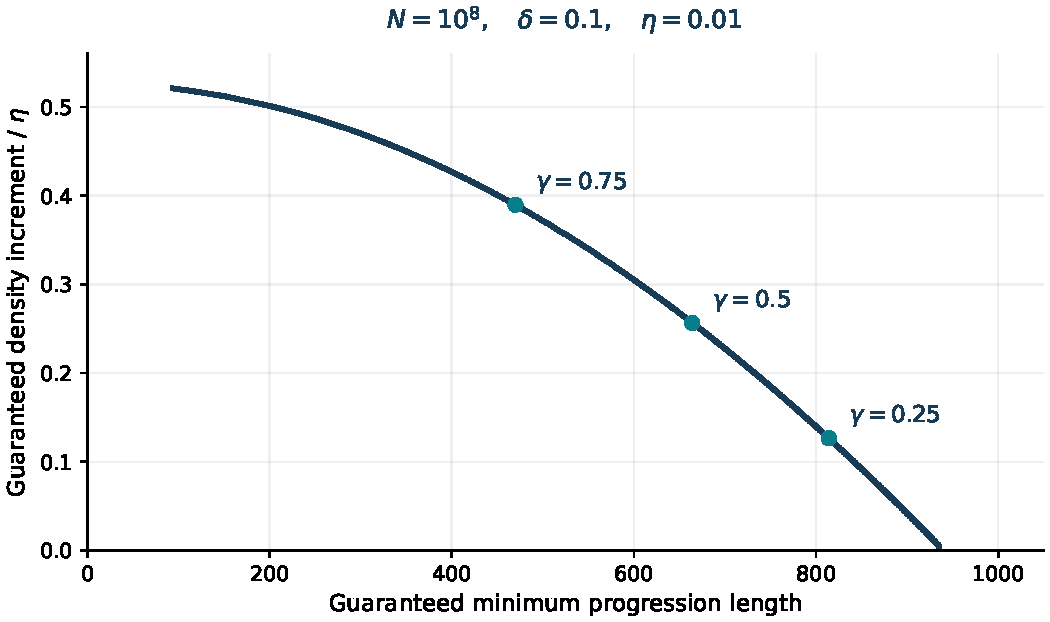
\includegraphics[width=0.92\textwidth]{figures/10-torsion-energy-phase_frontier.pdf}
\caption{The proved density--length tradeoff, evaluated at fixed
$N=10^8$, $\delta=0.1$, and normalized correlation $\eta=0.01$.
The vertical axis divides the guaranteed increment by $\eta$.
These points are evaluations of formulas, conditional on the
correlation hypothesis, rather than measurements of extremal sets.}
\label{gsr:dt:10:fig:phase-frontier}
\end{figure}

For a concrete comparison, the following table uses $\gamma=1/2$
and $N=10^8$ throughout.  The older length column evaluates the
continuous lower bound already present in the supplied proof; the
new length column includes the floor in \eqref{gsr:dt:10:eq:half-length}.
All three parameter choices satisfy the older large-scale condition.

\begin{center}\small
\begin{tabular}{@{}rr r r r r@{}}
\toprule
$\delta$ & $\eta$ & Older length & New length & Older gain & New gain\\
\midrule
$0.5$ & $0.05$ & $111.51$ & $892$ & $0.0125$ & $0.0128205$\\
$0.1$ & $0.01$ & $49.87$ & $664$ & $0.0025$ & $0.00256410$\\
$0.01$ & $0.0001$ & $4.99$ & $200$ & $0.000025$ & $0.0000250627$\\
\bottomrule
\end{tabular}
\end{center}

The improvement in the length guarantee is especially visible at low
density because the phase approximation error is charged to
$\mathbb E|\mathbf1_A-\delta|=2\delta(1-\delta)$.  Each entry is
conditional on the presence of the specified Fourier coefficient;
the table does not claim that an arbitrary set of the given density
has such a coefficient.
\begin{writenote}[6 October 2026; sources 06--10]
Corollary~\ref{gsr:dt:10:cor:half} has exactly source~01's length \eqref{gsr:dt:01:eq:finalL} and source~05's increment $\delta\eta/(4\delta-\eta)$ (Theorem~\ref{gsr:dt:05:thm:density}), so source~01's Theorem~\ref{gsr:dt:01:thm:fourier} gives an increment at least $3/2$ times as large at the same length; along the frontier of Theorem~\ref{gsr:dt:10:thm:frontier} the comparison holds for $\gamma\le1/2$ and changes at $\gamma=3/(4-\kappa)$ (proof in the note after Table~\ref{gsr:dt:01:tab:increment}). The repository's proof-level pair of Corollary~2.5 is \file{cor25_large_scale} (\file{Proofs02DensityIncrement.lean}); not formalized.
\end{writenote}


\subsection{Using the exact variance in the \texorpdfstring{$U^2$}{U2} inverse step}

\begin{proposition}\label{gsr:dt:10:prop:u2-variance}
Let $A$ be a set of density $\delta\in(0,1)$ in a finite abelian group,
and $f=\mathbf1_A-\delta$.  Then
\[
 \max_{\chi\ne1}|\widehat f(\chi)|
 \geq\frac{\|f\|_{U^2}^{\,2}}{\sqrt{\delta(1-\delta)}}.
\]
More generally, a mean-zero function with $\|f\|_2^2=V>0$ has a
nontrivial Fourier coefficient of modulus at least $\|f\|_{U^2}^2/\sqrt V$.
\end{proposition}
\begin{proof}
Fourier orthogonality gives
$\|f\|_{U^2}^4=\sum_\chi|\widehat f(\chi)|^4$ and Parseval gives
$\sum_\chi|\widehat f(\chi)|^2=V$.  The trivial coefficient vanishes.
Bound one of the two quadratic factors in each fourth power by the
largest coefficient squared and divide by $V$.
\end{proof}

In a cyclic group, this may be substituted directly into
Corollary~\ref{gsr:dt:10:cor:half}.  It is a variance-sensitive version of the
standard $U^2$ inverse argument, not a replacement for the higher-order
inverse theorem.  The proof also explains why an apparent improvement
obtained solely by changing normalized to unnormalized Fourier
coefficients would be spurious.


% Integration requirements: amsmath, amssymb, amsthm; environments
% theorem, lemma, proposition, corollary.  No custom macros or citations.

\gsroldfloats
\clearpage
\part{The inverse step: energies, moments, restriction and dependent random choice}\label{gsr:en:part}
\partsource{
\textbf{Contents.} From many correlated derivatives to an approximate homomorphism. Sections~\ref{gsr:en:02:sec:d2}--\ref{gsr:en:02:sec:d5}: source~02, delivered Sections~2--5 (a sharp weighted, mixed-function extension of Proposition~6.1 on every finite abelian group, its equality cases, deficits and rigidity). Sections~\ref{gsr:en:03:sec:d7}--\ref{gsr:en:03:sec:d8}: source~03, delivered Sections~7--8 (a cubic dependent-random-choice certificate for Lemma~7.4, and an elementary replacement for Proposition~7.3). Sections~\ref{gsr:en:04:sec:d2}--\ref{gsr:en:04:sec:d5}: source~04, delivered Sections~2--5 (its notation; exact second moments for Lemma~9.2; a polynomial restriction theorem for Lemma~9.3 and Corollary~9.4 over prime fields; arrangement moments for Lemmas~12.4, 14.7 and~14.8). The three sources treat different steps; no statement is printed twice. Source~04's Section~\ref{gsr:en:04:sec:d2} also fixes the cube notation used by its Part~III sections.
}
\noindent\textbf{Reading conventions of this Part} (the full dictionary is Section~\ref{gsr:fm:sec:notation}).
\begin{center}\small
\begin{tabular}{@{}>{\raggedright\arraybackslash}p{0.17\textwidth} >{\raggedright\arraybackslash}p{0.78\textwidth}@{}}
\toprule
Symbol & Meanings in this Part, by source (\emph{tempting false reading} in italics)\\
\midrule
$\mathcal E$ & 02: $\calE(w)$, additive energy of a weight on $G\times\widehat G$, normalized by $N^{-3}$; 04: $\mathcal E_j(w)=M^{-1}\sum_\chi|\widehat w(\chi)|^{2j}$ with the \emph{unnormalized} transform, counting $2j$-tuples; 03: $E(A)$ the additive energy of a set. \emph{These are three different normalizations.}\\
$\U$, $T$ & 02: $\U(f)=\norm f_{U^3}^8$ (normalized), $\calT_w(f,g)$ a weighted derivative correlation, $T$ its graph case; 04: $T_d(B)$ and $T_d^\phi(B)$ counts of additive and respected $2d$-tuples.\\
$\kappa$, $\rho$, $m$ & 02: $\kappa=\U(f)/m(f)^4$, $m(f)=\E|f|^2$; 03: $\kappa=7/(3\sqrt6)$, $\kappa_*$, $\rho=c/(2-c)$, $m=|V|$ or $|A|$; 04: $\kappa_d=1/(2(400d)^d)$, $\rho=m/M$ with $m=|A|$.\\
$R$, $L$, $Q$ & 02: $R=\E|K_u(s)|^2$; 04: $R_j$ counts respected arrangements, $L$ the kernel bandwidth, $Q$ the kernel ratio sum (R14); 03: $L=|D|$. Source~04's tags (M1)--(M7), (R1)--(R32), (A1)--(A14) label displays: \emph{(R3) is a display, not a remainder $R_3$; (A1) is not Appendix~A}.\\
\bottomrule
\end{tabular}
\end{center}
\medskip
\begingroup\small\noindent\textbf{Added in the second write (6~October 2026): sources 06--10.} \textbf{Contents.} Sections~\ref{gsr:en:sec:transport}--\ref{gsr:en:07:sec:d8} are source~07's chapter: a guide written for this report (Section~\ref{gsr:en:sec:transport}), source~07's own notation table (its Appendix~A, placed first), and its delivered Sections~2--8 (finite fibered domains and the directional error law; transport profiles; the coupled-path rigidity theorem; the sharp balanced threshold $1/(2k)$; the application to Gowers's Section~10 with Freiman orders five and nine; the rational linear program for the starting law; collision-to-mode exactification, weighted laws and nonabelian groups). Sections~\ref{gsr:en:10:sec:d7}--\ref{gsr:en:10:sec:d8}: source~10, delivered Sections~7--8 (a weighted energy extraction with $(c/4,\,2^{10}c^{-5})$ in Proposition~7.3; the vertical-obstruction-fibre form of the Freiman extraction of Lemma~7.5, the order-eight retention $2^{-209}\gamma^{103}$ in Corollary~7.6, and a torsion budget for general finite codomains).

\textbf{Overlaps (dated notes).} Source~10's Theorem~\ref{gsr:en:10:thm:weighted-bsg} and source~03's Theorem~\ref{gsr:en:03:drc:elementary-bsg} are two elementary replacements of Proposition~7.3 under the same hypothesis; source~10's is stronger in both conclusions (note after source~03's theorem). Source~07 treats a step that no other source treats (Lemma~10.9); its relation to the Lean statement \file{lemma_10_9} is stated precisely in Section~\ref{gsr:en:sec:transport} and in the note after Corollary~\ref{gsr:en:07:cor:nine}.\par\endgroup
\medskip
\noindent\textbf{Reading conventions for the sections of sources 06--10 in this Part.}
\begin{center}\small
\begin{tabular}{@{}>{\raggedright\arraybackslash}p{0.17\textwidth} >{\raggedright\arraybackslash}p{0.78\textwidth}@{}}
\toprule
Symbol & Meanings in this Part, by source (\emph{tempting false reading} in italics)\\
\midrule
$\delta$, $\delta_d$, $b_d$ & 07: $\delta_d$ the directional defect of a direction $d$, $b_d$ its boundary mass, $\delta$ a uniform bound on the $\delta_d$. \emph{07's $\delta$ is a failure probability, not a density.}\\
$\mathcal T_s$, $\mathcal C$, $c(s)$ & 07: $\mathcal T_s(t)$ the transport profile, $\mathcal C(\mathbf d)$ the cost of a word, $c(s)$, $A(s)$, $M(s)$ the coarse envelopes, $\nu$ an alternative starting law. \emph{07's $\mathcal C$ is not the cube count $\mathcal C_d$ of 08 and 09 (Part~III).}\\
$\kappa$, $\tau$, $L$, $r_0$, $S$, $W$ & 07: $\kappa$ the fibre-size ratio, $L$ the one-step fibre-size variation, $r_0$ the internal lower bound, $\tau=L/r_0$; $S$ the usable support, $W$ the union of its fibres. \emph{07's $\kappa$ is none of the $\kappa$'s of 02, 03 and~04.}\\
$\theta$, $\eta$, $\alpha$, $\rho$, $\sigma$, $M$ & 07: the parameters of Gowers's Lemmas~10.6--10.9 and of \file{Section10.lean}: $\theta=10\eta^{1/5}$, $q(\theta)=2\theta-\theta^2$, $\Delta=q(\theta)+\eta$; $\alpha,\rho,\sigma,M$ in \eqref{gsr:en:07:eq:full-package} as there (\emph{$M$ is the fibre-size cap, not a modulus}). $\Fr_k(D,H)$: Freiman homomorphisms of order $k$, the definition of the Lean \texttt{FreimanHom}.\\
$E(A)$, $c$, $T(a,b)$ & 10: $E(A)=\sum_dr_A(d)^2$ and $c$ as in 03's Theorem~\ref{gsr:en:03:drc:elementary-bsg}; $w(a,b)$, $T(a,b)$ weighted codegrees, $K$ a random subset, $Z$ its bad pairs. \emph{10's $T$ is not 02's $T$.}\\
$\Gamma$, $H_k$, $h_k$, $\gamma$, $F$, $V$ & 10: $\Gamma$ a graph, $H_k$ its vertical obstruction fibre and $h_k=|H_k|$, $C$ a doubling constant, $\gamma$ the graph-energy proportion, $F$ the defect set and $V$ the codomain of Theorem~\ref{gsr:en:10:thm:torsion-fibre-extraction}. \emph{10's $h_k$ is not the $h_k=(k-2)2^{k-1}+1$ of Part~IV, and this $\gamma$ is not 10's $\gamma$ of Part~I.}\\
\bottomrule
\end{tabular}
\end{center}
\medskip
\section[{Normalization and finite Fourier identities\srctag{02}}]{Normalization and finite Fourier identities}\label{gsr:en:02:sec:d2}
\srcnote{02}{Section 2}
Let $G$ be a finite abelian group of order $N\geq1$, written additively, and let $\widehat G$ be its character group, written multiplicatively. Thus $(h,\chi)+(k,\psi)$ in $G\times\widehat G$ means $(h+k,\chi\psi)$. All averages over $G$ are normalized; sums over $\widehat G$ are not:
\[
 \E_x a(x)=\frac1N\sum_{x\in G}a(x),\qquad
 \widehat a(\chi)=\E_xa(x)\overline{\chi(x)}.
\]
Fourier orthogonality gives
\begin{equation}\label{gsr:en:02:eq:parseval}
 \E_x|a(x)|^2=\sum_{\chi\in\widehat G}|\widehat a(\chi)|^2.
\end{equation}
For normalized convolution $(a*b)(s)=\E_h a(s-h)b(h)$, we have $\widehat{a*b}=\widehat a\,\widehat b$. These facts follow by expanding the sums and using $\E_x\chi(x)=0$ for a nontrivial character and $1$ for the trivial character.

Define
\[
 \Delta_hf(x)=f(x)\overline{f(x-h)},\qquad m(f)=\E_x|f(x)|^2,
\]
and define the eighth power of the normalized $U^3$ norm by
\begin{equation}\label{gsr:en:02:eq:u3spectral}
 \U(f)=\E_h\sum_{\chi\in\widehat G}
              |\widehat{\Delta_hf}(\chi)|^4.
\end{equation}
It also equals the usual cube average
\begin{equation}\label{gsr:en:02:eq:u3cube}
 \E_{x,a,b,c}\prod_{\omega\in\{0,1\}^3}
  \mathcal C^{|\omega|} f(x+\omega_1a+\omega_2b+\omega_3c),
\end{equation}
where $\mathcal C$ denotes complex conjugation. One proof first expands the fourth Fourier moment in~\eqref{gsr:en:02:eq:u3spectral}; character orthogonality leaves the additive quadruple constraint, which is parameterized by three variables. The remaining derivative variable gives~\eqref{gsr:en:02:eq:u3cube}, after changes of signs in the increment variables. In particular $\U(f)$ is nonnegative.

For $f,g:G\to\C$, write
\[
 A_{f,g}(h,\chi)=\E_x f(x)\overline{g(x-h)}\overline{\chi(x)}.
\]
This is just a Fourier transform of a mixed derivative, not an additional assumption about $f$ or $g$.

\begin{definition}[Weighted correlation and energy]
For any $w:G\times\widehat G\to[0,\infty)$, define
\begin{align}
 \calT_w(f,g)&=\E_h\sum_\chi w(h,\chi)|A_{f,g}(h,\chi)|^2,
       \label{gsr:en:02:eq:Tdef}\\
 \calE(w)&=\frac1{N^3}
 \sum_{\substack{h_1+h_2=h_3+h_4\\
                 \chi_1\chi_2=\chi_3\chi_4}}
           \prod_{j=1}^4w(h_j,\chi_j). \label{gsr:en:02:eq:Edef}
\end{align}
\end{definition}
The factor $N^{-3}$ in~\eqref{gsr:en:02:eq:Edef} is deliberate: it normalizes the energy of a full additive graph to $1$. It is not the uniform-probability normalization on the group of order $N^2$. If $w=\one_\Gamma$, then $N^3\calE(w)$ is the ordinary ordered additive-quadruple count of $\Gamma$.

\section[{A sharp weighted extension of Proposition 6.1\srctag{02}}]{A sharp weighted extension of Proposition 6.1}\label{gsr:en:02:sec:d3}
\srcnote{02}{Section 3}

\begin{theorem}[Mixed energy-sensitive inverse step]\label{gsr:en:02:thm:main}
For every finite abelian group $G$, every $f,g:G\to\C$, and every nonnegative weight $w:G\times\widehat G\to[0,\infty)$,
\begin{equation}\label{gsr:en:02:eq:main}
 \boxed{\quad
 \calT_w(f,g)^4\leq
 \min\{m(f)^4\U(g),\ m(g)^4\U(f)\}\,\calE(w).
 \quad}
\end{equation}
There is no pointwise boundedness assumption on $f,g$, and no graph or bounded-fiber assumption on $w$. The coefficient $1$ cannot be decreased.
\end{theorem}

\subsection{Three exact identities}
For $u\in G$ define
\[
 F_u(s)=f(s)\overline{f(s-u)},\qquad
 D_u(s)=g(s)\overline{g(s-u)},\qquad
 V_u(h)=\sum_\chi w(h,\chi)\chi(u),
\]
and put $K_u=D_u*V_u$. Use the normalized inner product
\[
 \ip{F}{K}=\E_{u,s}F_u(s)\overline{K_u(s)}.
\]
Then
\begin{align}
 \calT_w(f,g)&=\ip{F}{K}, \label{gsr:en:02:eq:identity1}\\
 R:=\E_{u,s}|K_u(s)|^2
   &=\E_u\sum_\psi|\widehat D_u(\psi)|^2
                         |\widehat V_u(\psi)|^2, \label{gsr:en:02:eq:identity2}\\
 \E_u\sum_\psi|\widehat V_u(\psi)|^4&=\calE(w). \label{gsr:en:02:eq:identity3}
\end{align}
For~\eqref{gsr:en:02:eq:identity1}, expand the square in~\eqref{gsr:en:02:eq:Tdef}, set the second spatial variable equal to $s-u$, and obtain
\[
 \E_{u,s} f(s)\overline{f(s-u)}
 \E_h \overline{g(s-h)}g(s-u-h)
                  \sum_\chi w(h,\chi)\overline{\chi(u)}.
\]
This is exactly $\ip{F}{K}$. Nonnegativity of $w$ also makes the original expression visibly real and nonnegative. Identity~\eqref{gsr:en:02:eq:identity2} is Parseval and the convolution identity.

For~\eqref{gsr:en:02:eq:identity3}, expand
\[
 \widehat V_u(\psi)=\frac1N\sum_{h,\chi}
                  w(h,\chi)\chi(u)\overline{\psi(h)}.
\]
The fourth power contributes $N^{-4}$. Summing over $\psi$ contributes $N$ and imposes $h_1+h_2=h_3+h_4$. Averaging over $u$ imposes $\chi_1\chi_2=\chi_3\chi_4$ without another factor. The remaining normalization is $N^{-3}$, proving the identity.

\subsection{Proof of the theorem}
The first exact norm is
\[
 \|F\|_2^2=\E_{u,s}|f(s)|^2|f(s-u)|^2=m(f)^2.
\]
Cauchy--Schwarz applied to~\eqref{gsr:en:02:eq:identity1} therefore gives
\begin{equation}\label{gsr:en:02:eq:CS1}
 \calT_w(f,g)^2\leq m(f)^2R.
\end{equation}
Applying Cauchy--Schwarz to~\eqref{gsr:en:02:eq:identity2}, this time on the measure space with average in $u$ and counting measure in $\psi$, gives
\begin{equation}\label{gsr:en:02:eq:CS2}
 R^2\leq
 \left(\E_u\sum_\psi|\widehat D_u(\psi)|^4\right)
 \left(\E_u\sum_\psi|\widehat V_u(\psi)|^4\right)
 =\U(g)\calE(w).
\end{equation}
Squaring~\eqref{gsr:en:02:eq:CS1} and using~\eqref{gsr:en:02:eq:CS2} proves the first bound in~\eqref{gsr:en:02:eq:main}.

For the other bound, let $w^\vee(h,\chi)=w(-h,\chi^{-1})$. Directly changing variables in the mixed Fourier coefficient gives
\[
 |A_{f,g}(h,\chi)|=|A_{g,f}(-h,\chi^{-1})|.
\]
Consequently $\calT_w(f,g)=\calT_{w^\vee}(g,f)$. Inversion is an automorphism of the abelian group $G\times\widehat G$, so $\calE(w^\vee)=\calE(w)$. Apply the first bound with $f$ and $g$ exchanged. Equality examples establishing the final assertion are given in Section~\ref{gsr:en:02:sec:sharp}. \qed

\begin{corollary}[Graph version]\label{gsr:en:02:cor:graph}
Let $B\subseteq G$, $\phi:B\to\widehat G$, and $\Gamma=\{(h,\phi(h)):h\in B\}$. If
\[
 T=\E_h\one_B(h)|\widehat{\Delta_hf}(\phi(h))|^2>0,
\]
then, writing $E(\Gamma)$ for the unnormalized additive energy,
\begin{equation}\label{gsr:en:02:eq:graphbound}
 \frac{E(\Gamma)}{N^3}\geq\frac{T^4}{m(f)^4\U(f)}.
\end{equation}
In particular, the hypothesis~\eqref{gsr:fm:02:eq:old61} implies
\[
 E(\Gamma)\geq\frac{\alpha^4}{m(f)^4\U(f)}N^3.
\]
\end{corollary}
\begin{proof}
Take $g=f$ and $w=\one_\Gamma$. The unnormalized Fourier coefficient is $N$ times our normalized coefficient, so the statistic in~\eqref{gsr:fm:02:eq:old61}, divided by $N^3$, is precisely $T$. Positive $T$ makes the denominator nonzero by Theorem~\ref{gsr:en:02:thm:main}.
\end{proof}
\begin{writenote}[6 October 2026]
\emph{The formal statement is recovered.} The formal \file{proposition_6_1} (\file{Sections06\_07.lean}, line~37; exact companion \file{proposition_6_1_holds}, \file{Proofs05\_10.lean}, line~505) is the case $|f|\le1$ on $\Z_N$ with a single-valued graph: there $m(f)\le1$ and $\U(f)\le m(f)^4\le1$ (Lemma~\ref{gsr:en:02:lem:l2}), so \eqref{gsr:en:02:eq:graphbound} gives $E(\Gamma)\ge\alpha^4N^3$. The intake also tested Theorem~\ref{gsr:en:02:thm:main} on the non-cyclic groups $\Z/2\times\Z/4$ and $\Z/2\times\Z/2\times\Z/3$ and on $\Z/6$ (largest ratio of left to right side $0.084$); the delivered suite uses cyclic groups only. \emph{Notation:} this $\calE(w)$ is not source~03's $\mathcal E(f)$ (Part~III), source~04's $\mathcal E_j(w)$ (Section~\ref{gsr:en:04:sec:d3}) or source~05's captured energy $E$ (Part~I); see Section~\ref{gsr:fm:sec:notation}.
\end{writenote}

\section[{\texorpdfstring{The $L^2$ denominator and equality examples}{The L2 denominator and equality examples}\srctag{02}}]{The $L^2$ denominator and equality examples}\label{gsr:en:02:sec:d4}\label{gsr:en:02:sec:sharp}
\srcnote{02}{Section 4}

\begin{lemma}[Two tetrahedra]\label{gsr:en:02:lem:l2}
For every finite abelian group and every complex function on it,
\begin{equation}\label{gsr:en:02:eq:l2u3}
 \U(f)\leq m(f)^4,\qquad\text{equivalently}\qquad
 \|f\|_{U^3}\leq\|f\|_2.
\end{equation}
\end{lemma}
\begin{proof}
Take the absolute value of the cube average~\eqref{gsr:en:02:eq:u3cube}. Divide its eight factors into the four vertices
\[
 x,\quad x+a,\quad x+b,\quad x+c
\]
and the complementary four vertices
\[
 x+a+b,\quad x+a+c,\quad x+b+c,\quad x+a+b+c.
\]
Cauchy--Schwarz bounds the cube average by the geometric mean of the averages of the squared products on these two lists. The first list is a bijective change of coordinates from $G^4$ to $G^4$. The second is also bijective: if its coordinates are $y_1,y_2,y_3,y_4$, then
\[
 c=y_4-y_1,\quad b=y_4-y_2,\quad a=y_4-y_3,
 \quad x=y_1+y_2+y_3-2y_4.
\]
Thus each squared-product average is $m(f)^4$, proving~\eqref{gsr:en:02:eq:l2u3}. No division by $2$ occurs in the inverse map, so groups with $2$-torsion are included.
\end{proof}

\begin{corollary}[Variance-normalized energy]\label{gsr:en:02:cor:variance}
Whenever the denominator is nonzero,
\[
 \calE(w)\geq
 \left(\frac{\calT_w(f,g)}{m(f)m(g)}\right)^4.
\]
For a graph and a balanced indicator $f=\one_A-\delta$, where $\delta=|A|/N\in(0,1)$,
\begin{equation}\label{gsr:en:02:eq:balancedenergy}
 \boxed{\quad
 \frac{E(\Gamma)}{N^3}
 \geq\frac{T^4}{[\delta(1-\delta)]^4\U(f)}
 \geq\frac{T^4}{[\delta(1-\delta)]^8}.
 \quad}
\end{equation}
\end{corollary}
\begin{proof}
Use Lemma~\ref{gsr:en:02:lem:l2} in Theorem~\ref{gsr:en:02:thm:main}. For a balanced indicator, direct averaging gives $m(f)=\delta(1-\delta)$.
\end{proof}

The improvement in~\eqref{gsr:en:02:eq:balancedenergy} is not a change in the fourth power of $T$. It is the retention of an exact variance denominator, together with a possibly smaller $U^3$ denominator. It is therefore misleading to describe it as a new exponent in Szemer\'edi's theorem. It can nevertheless be a large improvement in a local energy ledger.

\begin{example}[Quadratic-phase graph]\label{gsr:en:02:ex:quadratic}
Let $G=\Z_p$ for an odd prime $p$, put $q(x)=\exp(2\pi i x^2/p)$, and let $f=cq$, $c\ne0$. Then
\[
 \Delta_hf(x)=|c|^2\exp\bigl(2\pi i(2hx-h^2)/p\bigr).
\]
Choose the graph $h\mapsto\chi_{2h}$. We have
\[
 m(f)=|c|^2,\quad \U(f)=|c|^8,\quad T=|c|^4,
 \quad E(\Gamma)=N^3.
\]
Equality holds in both~\eqref{gsr:en:02:eq:main} and the variance-normalized bound. In particular the coefficient $1$ in the main theorem is optimal even for a single-valued graph.
\end{example}

\begin{example}[A genuinely multivalued sharp example]\label{gsr:en:02:ex:rectangle}
Let $H\leq G$ have density $d=|H|/N$, let $f=\one_H$, and take $w=\one_{H\times H^\perp}$, where $H^\perp$ is the annihilator of $H$. The set $H\times H^\perp$ is a subgroup of $G\times\widehat G$ of size $N$, hence $\calE(w)=1$. Also
\[
 m(f)=d,\qquad \U(f)=d^4,\qquad \calT_w(f,f)=d^2.
\]
The cube formula gives $\U(f)=d^4$ because all eight vertices belong to $H$ exactly when the base and three increments do. The Fourier coefficient of $\one_H$ is $d$ on $H^\perp$ and $0$ elsewhere, giving the value of $\calT$. Again equality holds in the main theorem.
\end{example}

\begin{example}[Sharpness within balanced indicators]\label{gsr:en:02:ex:balanced}
On an even cyclic group, take $A$ to be the even residues. Then $f=\one_A-1/2$ is one half of a character. For the graph with trivial frequency at every $h$,
\[
 m(f)=\tfrac14,\qquad \U(f)=\tfrac1{256},\qquad
 T=\tfrac1{16},\qquad E(\Gamma)/N^3=1.
\]
The original $T^4$ bound is $1/65536$, whereas~\eqref{gsr:en:02:eq:balancedenergy} gives the exact value $1$. This demonstrates a strict strengthening on an admissible balanced input, not merely on arbitrary unbounded functions.
\end{example}

\section[{Keeping the full derivative spectrum and tracking rigidity\srctag{02}}]{Keeping the full derivative spectrum and tracking rigidity}\label{gsr:en:02:sec:d5}
\srcnote{02}{Section 5}

\subsection{A support-and-energy certificate without selecting one frequency}
\begin{proposition}\label{gsr:en:02:prop:spectrum}
Let $f\not\equiv0$, set $m=m(f)$ and $\kappa=\U(f)/m^4\in(0,1]$, and let $0<\tau\leq1$. Define
\[
 \Gamma_\tau=\{(h,\chi):|A_{f,f}(h,\chi)|\geq\tau m\},
 \qquad
 t_\tau=\frac{\calT_{\one_{\Gamma_\tau}}(f,f)}{m^2}.
\]
Then
\begin{align}
 |\Gamma_\tau|&\leq N\tau^{-2}, \label{gsr:en:02:eq:supportbad}\\
 \frac{E(\Gamma_\tau)}{N^3}&\geq\frac{t_\tau^4}{\kappa},\label{gsr:en:02:eq:spectralenergy}\\
 \frac{E(\Gamma_\tau)}{|\Gamma_\tau|^3}
   &\geq\frac{t_\tau^4\tau^6}{\kappa}
   \quad\text{if }\Gamma_\tau\ne\varnothing.\label{gsr:en:02:eq:relativeenergy}
\end{align}
\end{proposition}
\begin{proof}
Parseval, followed by averaging in $h$, gives the exact identity
\[
 \sum_{h,\chi}|A_{f,f}(h,\chi)|^2
 =N\E_{h,x}|f(x)|^2|f(x-h)|^2=Nm^2.
\]
This proves the support bound. Apply Theorem~\ref{gsr:en:02:thm:main} to the full set $\Gamma_\tau$, not a chosen graph, and substitute $\U(f)=\kappa m^4$. Finally divide by the cube of the support bound. Nonzero $f$ has $\U(f)>0$: the $h=0$ summand in~\eqref{gsr:en:02:eq:u3spectral} already has a nonzero Fourier coefficient.
\end{proof}

The certificate~\eqref{gsr:en:02:eq:relativeenergy} is suitable input for an additive-energy-to-structure theorem of Balog--Szemer\'edi--Gowers type. The subsequent structural step is not proved anew here. The point is that there is no preliminary loss from discarding all but one frequency in each fiber. Whether that benefit survives the later graph and progression constructions is a separate quantitative problem.

\subsection{Exact deficits in the two Cauchy--Schwarz steps}
With $F,D,V,K,R$ as in Section~\ref{gsr:en:02:sec:d3}, set
\[
 D_1=m(f)^2R-\calT_w(f,g)^2,\qquad
 D_2=\U(g)\calE(w)-R^2.
\]
Both are nonnegative, and direct algebra gives
\begin{equation}\label{gsr:en:02:eq:deficit}
 m(f)^4\U(g)\calE(w)-\calT_w(f,g)^4
 =m(f)^4D_2+D_1\bigl(m(f)^2R+\calT_w(f,g)^2\bigr).
\end{equation}
Thus the loss is decomposed exactly, rather than hidden in an unspecified constant.

\begin{proposition}[Quantitative alignment]\label{gsr:en:02:prop:stability}
Suppose all quantities used to normalize below are nonzero and $0\leq\varepsilon<1$. If
\[
 \calT_w(f,g)^4\geq
 (1-\varepsilon)m(f)^4\U(g)\calE(w),
\]
then
\begin{align*}
 \left\|\frac{F}{\|F\|_2}-\frac{K}{\|K\|_2}\right\|_2^2
 &\leq2\bigl(1-(1-\varepsilon)^{1/4}\bigr),\\
 \left\|\frac{a}{\|a\|_2}-\frac{b}{\|b\|_2}\right\|_2^2
 &\leq2\bigl(1-\sqrt{1-\varepsilon}\bigr),
\end{align*}
where $a(u,\psi)=|\widehat D_u(\psi)|^2$ and
$b(u,\psi)=|\widehat V_u(\psi)|^2$. The first norm uses normalized measure on $G^2$; the second uses average in $u$ and counting measure in $\psi$.
\end{proposition}
\begin{proof}
Let $A=\calT^2/(m(f)^2R)$ and $B=R^2/(\U(g)\calE(w))$. The proof of Theorem~\ref{gsr:en:02:thm:main} gives $A,B\in[0,1]$, and the hypothesis says $A^2B\geq1-\varepsilon$. Hence $A\geq\sqrt{1-\varepsilon}$ and $B\geq1-\varepsilon$. The normalized inner products of the first and second pairs are $\sqrt A$ and $\sqrt B$, respectively. They are real and nonnegative, by~\eqref{gsr:en:02:eq:identity1} and~\eqref{gsr:en:02:eq:identity2}. Apply $\|v-w\|^2=2-2\RePart\ip vw$ for unit vectors.
\end{proof}

This is an alignment theorem for the proof's intermediate functions, not a full classification of all near-extremal pairs $(f,w)$. The distinction matters: subgroup-localized examples and polynomial phases already occur, and broader extremizer theory is known~\cite{eisnertao}.

\subsection{An elementary exact rigidity endpoint}
\begin{proposition}\label{gsr:en:02:prop:maximal}
Let $f\not\equiv0$, and let $\phi:G\to\widehat G$ be defined on all of $G$. For its graph statistic, $T\leq m(f)^2$. Equality holds if and only if $f=cq$, with $|q|=1$, and for each $h$
\[
 \Delta_hq(x)=c_h\phi(h)(x),\qquad |c_h|=1.
\]
In this situation $\phi$ is a homomorphism and all third multiplicative derivatives of $q$ equal $1$.
\end{proposition}
\begin{proof}
The chosen Fourier coefficient in each fiber has squared magnitude at most the sum of squared magnitudes in that fiber. The sum of all fibers is $m(f)^2$ after normalized averaging, by Parseval. Equality forces every $\Delta_hf$ to have Fourier support at the chosen single character. At $h=0$, $\Delta_0f=|f|^2$ is nonnegative and has positive mean. Its sole character must therefore be trivial, and $|f|^2=m(f)$ everywhere. Write $f=cq$ with $|q|=1$. Fourier inversion gives the stated derivative formula. Conversely that formula makes Parseval an equality in every fiber.

The identity
\[
 \Delta_{h+k}q(x)=\Delta_hq(x)\Delta_kq(x-h)
\]
shows that $\phi(h+k)=\phi(h)\phi(k)$, since a nonzero scalar multiple of a character has a unique character frequency. A further derivative of a character is constant, and a derivative of a unit-modulus constant is $1$; therefore third derivatives vanish multiplicatively. This definition of a quadratic phase does not impose an unjustified classical-polynomial representation in small characteristic.
\end{proof}

\section[{Sharper common-neighborhood selection\srctag{03}}]{Sharper common-neighborhood selection}\label{gsr:en:03:sec:d7}\label{gsr:en:03:drc:section}
\srcnote{03}{Section 7}

Gowers' Lemma~7.4 is a convenient place to make a concrete quantitative
improvement without changing the combinatorial objects in the argument.
Its hypothesis controls the average intersection of a family of sets; its
conclusion finds a subfamily in which almost every pair has a reasonably
large intersection.  The published proof samples five witnesses and
estimates the useful and exceptional contributions separately
\cite{gowers}.  Keeping those contributions together allows three
witnesses to suffice.

The method remains dependent random choice, whose subsequent development
is surveyed by Fox and Sudakov \cite{foxsudakov}.  Our assertion here
is a precise replacement for the numerical statement in the source paper.
We do not assert that the resulting exponent is optimal among all possible
selection arguments.

\subsection{A cubic certificate}

All pairs below are ordered, and diagonal pairs are included.  For a
finite family $A_1,\ldots,A_n$ of subsets of a set $V$ of cardinality $m>0$,
write
\[
 p_{xy}=\frac{\abs{A_x\cap A_y}}{m}.
\]
A pair will be called bad when $p_{xy}<a/2$, where $a>0$ is the specified
lower bound for the mean of the $p_{xy}$.

\begin{lemma}[Rational cubic certificate]\label{gsr:en:03:drc:cubic-certificate}
For every $a>0$ and $p\geq0$, define
\[
 F_a(p)=
 \begin{cases}
 -9p^3,&0\leq p<a/2,\\
 p^3,&p\geq a/2.
 \end{cases}
\]
Then
\begin{equation}\label{gsr:en:03:drc:certificate}
 F_a(p)\geq \frac{49}{12}a^2p-\frac{343}{108}a^3.
\end{equation}
\end{lemma}

\begin{proof}
On the good region $p\geq a/2$, the desired inequality is the tangent-line
inequality for $p^3$ at $p=7a/6$.  More explicitly,
\[
 p^3-\frac{49}{12}a^2p+\frac{343}{108}a^3
 =\left(p-\frac{7a}{6}\right)^2
   \left(p+\frac{7a}{3}\right)\geq0.
\]
On the interval $0\leq p\leq a/2$, the function
\[
 -9p^3-\frac{49}{12}a^2p+\frac{343}{108}a^3
\]
is concave, so its minimum on that interval occurs at an endpoint.  Its
values at $0$ and $a/2$ are, respectively,
\[
 \frac{343}{108}a^3
 \quad\hbox{and}\quad
 \frac{-243-441+686}{216}a^3=\frac{a^3}{108}.
\]
Both are positive.  At $p=a/2$, the actual function $F_a$ takes the larger,
good-region value, so the strict definition of a bad pair presents no
boundary issue.
\end{proof}

\begin{theorem}[Cubic replacement for Gowers' Lemma~7.4]
\label{gsr:en:03:drc:cubic-selection}
Let $m,n$ be positive integers, let $V$ have cardinality $m$, and let
$0<\delta\leq1$.  Suppose that $A_1,\ldots,A_n\subseteq V$ satisfy
\begin{equation}\label{gsr:en:03:drc:mean-hypothesis}
 \sum_{x,y=1}^n\abs{A_x\cap A_y}\geq\delta^2mn^2.
\end{equation}
There is a set $K\subseteq\{1,\ldots,n\}$ such that
\begin{equation}\label{gsr:en:03:drc:cubic-size}
 \abs K\geq\frac{7}{3\sqrt6}\,\delta^3n,
\end{equation}
and at least $90\%$ of the pairs $(x,y)\in K^2$ satisfy
\begin{equation}\label{gsr:en:03:drc:good-threshold}
 \abs{A_x\cap A_y}\geq\frac{\delta^2m}{2}.
\end{equation}
In particular, the conclusion holds when every $A_x$ has cardinality at
least $\delta m$.
\end{theorem}

\begin{proof}
Put $a=\delta^2$.  Independently sample $j_1,j_2,j_3$ uniformly from $V$,
allowing repetitions, and set
\[
 K=\{x:j_1,j_2,j_3\in A_x\}.
\]
Let $B(K)$ count the bad ordered pairs in $K^2$.  The probability that
$(x,y)\in K^2$ is $p_{xy}^3$.  Consequently, linearity of expectation
gives the exact identity
\begin{align*}
 \E\bigl[\abs K^2-10B(K)\bigr]
 &=\sum_{x,y=1}^n F_a(p_{xy})\\
 &\geq\frac{49}{12}a^2\sum_{x,y=1}^n p_{xy}
       -\frac{343}{108}a^3n^2\\
 &\geq\left(\frac{49}{12}-\frac{343}{108}\right)a^3n^2
  =\frac{49}{54}a^3n^2.
\end{align*}
The first inequality is Lemma~\ref{gsr:en:03:drc:cubic-certificate}; the second uses
\eqref{gsr:en:03:drc:mean-hypothesis}.  Some realization therefore satisfies
\[
 \abs K^2-10B(K)\geq\frac{49}{54}\delta^6n^2>0.
\]
It follows simultaneously that $\abs K\geq\sqrt{49/54}\,\delta^3n$ and
$B(K)\leq\abs K^2/10$.  These are the required conclusions.

For the final assertion, put $d(v)=\abs{\{x:v\in A_x\}}$.  Then
\[
 \sum_{x,y}\abs{A_x\cap A_y}
 =\sum_{v\in V}d(v)^2
 \geq\frac{1}{m}\left(\sum_{v\in V}d(v)\right)^2
 \geq\delta^2mn^2,
\]
by Cauchy--Schwarz and the assumed lower bounds on $\abs{A_x}$.
\end{proof}

The constant $7/(3\sqrt6)$ is approximately $0.95258$.  Thus the original
$2^{-1/2}\delta^5n$ is replaced by a larger bound with exponent $3$, while
both the half-mean intersection threshold and the $90\%$ requirement are
preserved.  The improvement comes from a stronger estimate of the same
penalized random variable, rather than from a change in the definition of
success.
\begin{writenote}[6 October 2026]
\emph{Compared with the formal statement} (checked at HEAD): \file{lemma_7_4} (\file{Sections06\_07.lean}, line~167) has the exact companion \file{lemma_7_4_holds} (\file{Proofs07DRC.lean}, line~536), which samples five witnesses indexed by \texttt{Fin 5}, as Section~\ref{gsr:fz:03:sec:formal} describes. Theorem~\ref{gsr:en:03:drc:cubic-selection} keeps its hypothesis, the threshold $\delta^2m/2$ and the $90\%$ requirement, and replaces the size $2^{-1/2}\delta^5n$ by $7\delta^3n/(3\sqrt6)$. Not formalized.
\end{writenote}

\subsection{Weights and higher tuples}

The certificate is independent of the counting measure on the index set.
This gives a useful extension when vertices carry unequal importance or
when intersections of more than two sets are under consideration.

\begin{corollary}[Weighted tuple selection]\label{gsr:en:03:drc:weighted}
Let $X$ be a finite nonempty set, let $w_x\geq0$ with
$\sum_{x\in X}w_x=1$, and let $(A_x)_{x\in X}$ be measurable subsets of a
probability space $(\Omega,\nu)$.  Fix an integer $r\geq1$, and suppose
\[
 \sum_{(x_1,\ldots,x_r)\in X^r}
   w_{x_1}\cdots w_{x_r}
   \nu(A_{x_1}\cap\cdots\cap A_{x_r})\geq a>0.
\]
There is a set $K\subseteq X$ with
\[
 w(K):=\sum_{x\in K}w_x
 \geq\left(\frac{49}{54}\right)^{1/r}a^{3/r}
\]
such that the total product weight of tuples in $K^r$ with
$\nu(A_{x_1}\cap\cdots\cap A_{x_r})<a/2$ is at most
$w(K)^r/10$.
\end{corollary}

\begin{proof}
Sample three independent points of $\Omega$ and let $K$ be the indices of
the sets containing all three points.  A fixed tuple lies in $K^r$ with
probability $p^3$, where $p$ is its intersection measure.  Apply
\eqref{gsr:en:03:drc:certificate} to each tuple and sum with its product weight.
The expected value of $w(K)^r$ minus ten times the bad-tuple weight is at
least $49a^3/54$.  Since $X$ is finite, there are only finitely many possible
sets $K$, and one attains at least this expectation.  Taking an $r$th root
gives the conclusion.
\end{proof}

\subsection{The exact scalar optimization}

The simple rational point $7a/6$ was chosen to make the certificate easy to
verify.  One can determine the optimal supporting line for this argument.
Let $z>1$ be the unique solution of
\begin{equation}\label{gsr:en:03:drc:z-root}
 2z^3-3z^2=9.
\end{equation}
The line tangent to $p^3$ at $p=za/2$ passes through the limiting bad point
$(a/2,-9a^3/8)$.  Applying that line instead of
\eqref{gsr:en:03:drc:certificate} gives
\begin{equation}\label{gsr:en:03:drc:optimized-constant}
 \abs K\geq\kappa_*\delta^3n,
 \qquad
 \kappa_*=\sqrt{\frac{3z^2-z^3}{4}}
          =0.9537881585\ldots.
\end{equation}
Indeed, the tangent has slope $3(za/2)^2$ and intercept $-2(za/2)^3$.
Equation~\eqref{gsr:en:03:drc:z-root} verifies its value at the bad endpoint.
Concavity on the bad interval and convexity on the good interval again
prove a global minorant.  Its value at the mean $a$ is
$(3z^2-z^3)a^3/4$.  Existence and uniqueness of $z>1$ follow from the fact
that $2z^3-3z^2$ is strictly increasing on $(1,\infty)$, starts at $-1$,
and tends to infinity. Moreover $2<z<5/2$, so the expression under
the square root is positive.

For clarity, the meaning of optimality here is limited and exact.  When
$za/2\leq1$, consider arbitrary scalar random variables $P\in[0,1]$ with
$\E P=a$.  A two-point distribution, with one value tending to $(a/2)^-$
and the other equal to $za/2$, approaches the tangent-line lower bound
for $\E F_a(P)$.  Thus no larger bound follows from this scalar mean
constraint alone.  The infimum is approached because badness is defined
by a strict inequality.

This observation also explains a restriction of a two-witness version
of the same argument.  Its penalized scalar function is $p^2$ on the good
region and $-9p^2$ on the bad region.  The analogous tangent point is
$ha$, where $h=(1+\sqrt{10})/2$.  The tangent's value at $a$ is
\[
 (2h-h^2)a^2<0.
\]
For sufficiently small $a$, the corresponding two-point distribution
lies in $[0,1]$ and gives a negative limiting expectation.  Consequently,
two witnesses and this scalar first-moment certificate cannot produce a
positive uniform lower bound at the original parameters.  This does not
exclude a better theorem exploiting properties of actual intersection
matrices, nor does it prove optimality of the exponent $3$.

\subsection{A flexible one-witness alternative}

For applications, keeping the threshold exactly at half the mean may be
unnecessary.  Allowing a smaller constant multiple of the mean gives a
much larger selected set using just one witness.  This is an explicit
form of the established variant in Fox and Sudakov
\cite[Lemma~5.1]{foxsudakov}.

\begin{lemma}[One-witness tradeoff]\label{gsr:en:03:drc:one-witness}
Under \eqref{gsr:en:03:drc:mean-hypothesis}, let $0<\gamma<\varepsilon<1$.
There is a set $K\subseteq\{1,\ldots,n\}$ satisfying
\[
 \abs K\geq\sqrt{1-\gamma/\varepsilon}\,\delta n
\]
such that at most an $\varepsilon$ fraction of the ordered pairs in
$K^2$ have intersection smaller than $\gamma\delta^2m$.
\end{lemma}

\begin{proof}
Choose $j\in V$ uniformly and set $K=\{x:j\in A_x\}$.  Then
\[
 \E\abs K^2=\sum_{x,y}p_{xy}\geq\delta^2n^2.
\]
If $B(K)$ counts the pairs in $K^2$ with
$p_{xy}<\gamma\delta^2$, then
\[
 \E B(K)=\sum_{p_{xy}<\gamma\delta^2}p_{xy}
 \leq\gamma\delta^2n^2.
\]
Thus
\[
 \E\bigl[\abs K^2-\varepsilon^{-1}B(K)\bigr]
 \geq(1-\gamma/\varepsilon)\delta^2n^2>0.
\]
A realization attaining at least this expectation gives both claims.
\end{proof}

\section[{An elementary quantitative replacement for Proposition~7.3\srctag{03}}]{An elementary quantitative replacement for Proposition~7.3}\label{gsr:en:03:sec:d8}
\srcnote{03}{Section 8}
\label{gsr:en:03:drc:bsg-section}

The preceding selection statements have different uses.  The cubic
version strengthens the exact statement of Lemma~7.4.  The one-witness
version is more efficient for the later small-difference-set argument,
because that argument can tolerate a smaller absolute constant in the
common-neighbor threshold.  We also remove a separate loss by counting
the total mass of popular differences directly.

Throughout this section, $A$ is a finite nonempty subset of an arbitrary
abelian group and $m=\abs A$.  Put
\[
 r_A(d)=\abs{\{(a,b)\in A^2:a-b=d\}},
 \qquad E(A)=\sum_d r_A(d)^2.
\]
We assume $E(A)\geq cm^3$, where $0<c\leq1$.  The sums involve only
finitely many nonzero terms, so no finiteness assumption on the ambient
group is required.

\subsection{Popular differences retain more edge mass}

\begin{lemma}[Popular mass]\label{gsr:en:03:drc:popular-mass}
Let
\[
 D=\{d:r_A(d)\geq cm/2\},\qquad
 M=\sum_{d\in D}r_A(d),\qquad \rho=\frac{c}{2-c}.
\]
Then $D=-D$, $\abs D\leq2m/c$, and $M\geq\rho m^2$.
\end{lemma}

\begin{proof}
The symmetry follows from $r_A(d)=r_A(-d)$.  Since
$\sum_d r_A(d)=m^2$, the lower bound $r_A(d)\geq cm/2$ on $D$ gives
$\abs D\leq2m/c$.  On $D$ we have $r_A(d)^2\leq m r_A(d)$, while off
$D$ we have $r_A(d)^2\leq(cm/2)r_A(d)$.  Therefore
\[
 cm^3\leq E(A)\leq mM+\frac{cm}{2}(m^2-M).
\]
Rearranging proves $M\geq cm^2/(2-c)$.
\end{proof}

This estimate retains the edge density of the popular-difference
relation.  It avoids the loss from first counting popular values and
then replacing each of their multiplicities by the smallest allowed
multiplicity.  In particular, the relation has density at least
$\rho\geq c/2$.

\subsection{A general walk-counting statement}

\begin{proposition}[Compression by four edge differences]
\label{gsr:en:03:drc:graph-compression}
Let $G\subseteq A\times A$ be a symmetric relation, with loops allowed,
satisfying $\abs G\geq\rho m^2$, where $0<\rho\leq1$.  Suppose that
every $(a,b)\in G$ has $a-b\in D$ for a finite set $D$, and put $L=\abs D$.
For $0<\gamma<\varepsilon<\beta<1/2$, set
$s=\sqrt{1-\gamma/\varepsilon}$.  There is $A'\subseteq A$ such that
\begin{align}
 \abs{A'}&\geq(1-\varepsilon/\beta)s\rho m,
 \label{gsr:en:03:drc:graph-size}\\
 \abs{A'-A'}&\leq
 \frac{L^4}{(1-2\beta)\gamma^2s\rho^5m^3}.
 \label{gsr:en:03:drc:graph-difference}
\end{align}
\end{proposition}

\begin{proof}
Write $N(a)=\{v:(a,v)\in G\}$.  By symmetry, double-counting, and
Cauchy--Schwarz,
\[
 \sum_{a,b\in A}\abs{N(a)\cap N(b)}
 =\sum_{v\in A}\abs{N(v)}^2
 \geq\frac{\abs G^2}{m}\geq\rho^2m^3.
\]
Lemma~\ref{gsr:en:03:drc:one-witness} supplies $U\subseteq A$, of cardinality
$u\geq s\rho m$, with at most $\varepsilon u^2$ bad ordered pairs.
Here a pair is bad when its common $G$-neighborhood has cardinality
smaller than $\gamma\rho^2m$.

Let $A'$ consist of the vertices of $U$ that belong, in the first
coordinate, to at most $\beta u$ bad pairs in $U^2$.  Counting those
pairs shows that at most $(\varepsilon/\beta)u$ vertices are excluded.
This proves \eqref{gsr:en:03:drc:graph-size}.  Each $a\in A'$ has at least
$(1-\beta)u$ good partners in $U$.  Consequently, every $a,b\in A'$ have
at least $(1-2\beta)u$ common good partners $k\in U$.

Fix such $a,b$.  For every common good partner $k$, choose
\[
 x\in N(a)\cap N(k),\qquad y\in N(b)\cap N(k).
\]
There are at least $(1-2\beta)u(\gamma\rho^2m)^2$ triples $(k,x,y)$.
Associate to each the four edge differences
\[
 d_1=a-x,\quad d_2=k-x,\quad d_3=k-y,\quad d_4=b-y.
\]
They lie in $D$ and satisfy
\[
 a-b=d_1-d_2+d_3-d_4.
\]
For the fixed endpoints $a,b$, the association is injective: one
recovers successively $x=a-d_1$, $k=x+d_2$, and $y=k-d_3$.

For each element of $A'-A'$, fix one pair of endpoints representing it.
The associated label quadruples for distinct differences are disjoint,
because a label quadruple determines $d_1-d_2+d_3-d_4$.  Since there are
only $L^4$ possible label quadruples,
\[
 \abs{A'-A'}(1-2\beta)u\gamma^2\rho^4m^2\leq L^4.
\]
Using $u\geq s\rho m$ proves \eqref{gsr:en:03:drc:graph-difference}.  This counts
walks with specified endpoints; repeated vertices and loops are allowed
throughout, and cause no loss in the injection.
\end{proof}

\subsection{Explicit bounds and their scope}

\begin{theorem}[Elementary historical improvement]\label{gsr:en:03:drc:elementary-bsg}
If $E(A)\geq c\abs A^3$ with $0<c\leq1$, there is $A'\subseteq A$
satisfying
\begin{equation}\label{gsr:en:03:drc:bsg-simple}
 \abs{A'}\geq\frac{c}{8}\abs A,
 \qquad
 \abs{A'-A'}\leq2^{19}c^{-9}\abs A.
\end{equation}
More precisely, with $\rho=c/(2-c)$, one may take
\begin{equation}\label{gsr:en:03:drc:bsg-precise}
 \abs{A'}\geq\frac{\rho m}{2\sqrt2},
 \qquad
 \abs{A'-A'}\leq6912\sqrt2\,\rho^{-5}c^{-4}m.
\end{equation}
\end{theorem}

\begin{proof}
Use $D$ from Lemma~\ref{gsr:en:03:drc:popular-mass}, and define
$G=\{(a,b)\in A^2:a-b\in D\}$.  That lemma gives
$\abs G\geq\rho m^2$ and $L\leq2m/c$.  Apply
Proposition~\ref{gsr:en:03:drc:graph-compression} with
\[
 \gamma=\frac1{12},\qquad \varepsilon=\frac16,\qquad
 \beta=\frac13,\qquad s=\frac1{\sqrt2}.
\]
The size bound is $\rho m/(2\sqrt2)$, and the difference bound becomes
\[
 \abs{A'-A'}
 \leq\frac{432\sqrt2\,L^4}{\rho^5m^3}
 \leq6912\sqrt2\,\rho^{-5}c^{-4}m.
\]
Finally $\rho\geq c/2$, so
\[
 \abs{A'}\geq\frac{cm}{4\sqrt2}\geq\frac{cm}{8},
 \qquad
 \abs{A'-A'}\leq221184\sqrt2\,c^{-9}m
 <2^{19}c^{-9}m.
\]
This proves both versions.
\end{proof}

For comparison, Proposition~7.3 in the source paper gives a subset of
size at least $2^{-20}c^{12}m$ with difference set of size at most
$2^{38}c^{-24}m$ \cite{gowers}.  Theorem~\ref{gsr:en:03:drc:elementary-bsg}
improves both exponents using only one sampled vertex, Cauchy--Schwarz,
and the explicit counting injection above.  Even if one changes only
Lemma~7.4 to Theorem~\ref{gsr:en:03:drc:cubic-selection} and leaves the remaining
original proof intact, its formulas yield the weaker but direct
improvements
\[
 \abs{A'}\geq2^{-14}c^8m,
 \qquad \abs{A'-A'}\leq2^{31}c^{-20}m.
\]
Indeed, the original parameter $\delta=c^2/8$ then gives selected density
$\alpha=\kappa\delta^4$, where $\kappa=7/(3\sqrt6)$; the original cleanup
and walk count give $\alpha m/2$ and
$120m/(\alpha\delta^4c^4)$, respectively.  The displayed relaxations use
$\kappa>1/2$ and $120/\kappa<128$.
\begin{writenote}[6 October 2026; sources 06--10]
\emph{A stronger elementary replacement (source~10).} Under the same hypothesis $E(A)\ge c|A|^3$, $0<c\le1$, source~10's Theorem~\ref{gsr:en:10:thm:weighted-bsg} gives $|A_*|\ge cm/4$ and $|A_*-A_*|\le2^{10}c^{-5}m$, on any abelian group, by weighted dependent random choice with the diagonal pairs kept. It is stronger than \eqref{gsr:en:03:drc:bsg-simple} in both conclusions: $c/4>c/8$, and $2^{10}c^{-5}\le2^{19}c^{-9}$ because $c^4\le1\le2^9$. Both are far weaker than Reiher--Schoen \cite{reiherschoen}, as both sources say. Both imply the formal \file{proposition_7_3} bounds $2^{-20}c^{12}$ and $2^{38}c^{-24}$ (for source~10: $c^{11}\le2^{18}$ and $c^{19}\le2^{28}$); neither is formalized. Lemma~7.4 is treated only here.
\end{writenote}

These are improvements to the historical proof architecture, rather
than to the strongest available Balog--Szemer\'edi--Gowers theorem.
For example, Reiher and Schoen prove that, for every $0<\eta<1/2$, the
same energy hypothesis gives a subset satisfying
\[
 \abs{A'}\geq(1-\eta)c^{1/2}m,
 \qquad
 \abs{A'-A'}\leq2^{33}\eta^{-9}c^{-4}\abs{A'}
\]
\cite[Theorem~1.2]{reiherschoen}.  Their result is substantially
stronger.  The purpose of the elementary version is to supply a short,
fully explicit replacement that can be checked independently and
integrated into the existing development with a small dependency set.
A complete improvement to the final quantitative Szemer\'edi bound would
also require propagating the new parameters through the later
arguments; no such consequence follows from this section alone.
\begin{writenote}[6 October 2026]
\emph{Compared with the formal statement} (checked at HEAD): \file{proposition_7_3} (\file{Sections06\_07.lean}, line~135; exact companion \file{proposition_7_3_holds}, \file{Proofs07BalogSzemeredi.lean}, line~996) is stated on $\Z^n$ with the bounds $2^{-20}c^{12}|A|$ and $2^{38}c^{-24}|A|$. For $0<c\le1$, $c/8\ge2^{-20}c^{12}$ (as $c^{11}\le2^{17}$) and $2^{19}c^{-9}\le2^{38}c^{-24}$ (as $c^{15}\le2^{19}$), so Theorem~\ref{gsr:en:03:drc:elementary-bsg}, which holds in every abelian group, implies the bounds of the formal statement. Not formalized.
\end{writenote}

\section[{Notation and normalization\srctag{04}}]{Notation and normalization}\label{gsr:en:04:sec:d2}
\srcnote{04}{Section 2}
\label{gsr:en:04:sec:notation}

Let \(G\) be a finite abelian group, written additively, and let \(N=|G|\).
We write \(\E_{x\in G}g(x)=N^{-1}\sum_{x\in G}g(x)\).
Characters are written multiplicatively.  Except in the moment section,
which explicitly introduces an unnormalized transform, Fourier
coefficients are normalized:
\[
 \widehat f(\chi)=\E_x f(x)\overline{\chi(x)}.
\]
Thus
\[
 \E_x|f(x)|^2=\sum_{\chi\in\widehat G}|\widehat f(\chi)|^2.
\]
Sums over the dual group in this convention are ordinary sums, not
averages.

For \(d\geq1\), put
\[
 \norm f_{U^d(G)}^{2^d}
 =\E_{x,h_1,\ldots,h_d}
   \prod_{\epsilon\in\{0,1\}^d}
    \mathcal C^{|\epsilon|}
    f(x+\epsilon_1h_1+\cdots+\epsilon_dh_d),
\]
where \(\mathcal C\) is complex conjugation.  We omit \(G\) when it is clear.
For \(d=1\) this means \(\norm f_{U^1}=|\E f|\).
For \(d\geq2\) it is the Gowers norm.  If \(f\) is real, conjugations can
be omitted.

For a real function \(w\), define its normalized cube count
\[
 Q_d(w)=
 \E_{x,h_1,\ldots,h_d}\prod_{\epsilon\in\{0,1\}^d}
     w(x+\epsilon\cdot h).
\]
For \(w=1_A\), \(N^{d+1}Q_d(w)\) counts all ordered additive
\(d\)-cubes, including degenerate cubes, exactly as in the corresponding
count in the source.  If \(\delta=|A|/N\), its balanced function is
\(f=1_A-\delta\).

The conversion to Gowers's parameter is important:
\[
 \text{\(f\) is \(\alpha\)-uniform of degree \(d-1\)}
 \quad\Longleftrightarrow\quad
 \norm f_{U^d}^{2^d}\leq\alpha.
\]
In particular, the letter \(u\) below generally denotes a norm, while
\(\alpha\) denotes an upper bound on a power of that norm.  Confusing these
two quantities would conceal the improvement in the exponent.

We use the standard Gowers--Cauchy--Schwarz inequality in normalized form:
\[
 \left|
 \E_{x,h}\prod_{\epsilon}
  \mathcal C^{|\epsilon|}f_\epsilon(x+\epsilon\cdot h)
 \right|
 \leq\prod_\epsilon\norm{f_\epsilon}_{U^d}.
\]
It follows by applying Cauchy--Schwarz successively in the cube
coordinates; this is Lemma~3.8 in the source.
Its ordinary consequences include the triangle inequality and
\(\norm f_{U^d}\leq\norm f_{U^{d+1}}\).
For clarity, the latter also follows by writing
\[
 \norm f_{U^d}^{2^d}
 =\E_{h_1,\ldots,h_{d-1}}
   \left|\E_x\Delta_{h_1}\cdots\Delta_{h_{d-1}}f(x)\right|^2.
\]
Square this identity and use Cauchy--Schwarz, then apply
\(|\E g|^4\leq\norm g_{U^2}^4\) to each derivative.  The resulting
right-hand side is \(\norm f_{U^{d+1}}^{2^{d+1}}\).

An ordered additive \(2d\)-tuple of a set \(B\) is a tuple with
\(x_1+\cdots+x_d=x_{d+1}+\cdots+x_{2d}\).
A map \(\phi:B\to H\) \emph{respects} the tuple if the same equation holds
after applying \(\phi\).  All tuple counts in this article are ordered
and allow repetitions unless expressly called nonexceptional.


% ===== moments =====

\section[{Exact second moments and density-sensitive lifting\srctag{04}}]{Exact second moments and density-sensitive lifting}\label{gsr:en:04:sec:d3}
\srcnote{04}{Section 3}
\label{gsr:en:04:mom:section}

Several losses in the paper occur when a second moment is bounded using
the size of the ambient space rather than the size of the set under
consideration.  Retaining the exact second moment is useful on its own,
and becomes particularly effective when followed by the restriction
argument in the next section.  The underlying interpolation inequality
is standard H\"older; the contribution here is the careful normalization,
the resulting sharper statements, and their use in the subsequent
selection theorem.

\subsection{Weighted energies on finite abelian groups}

Let \(H\) be a finite abelian group of order \(M\), and let
\(\widehat H\) be its character group.  For \(w:H\to\C\), use the
unnormalized transform
\[
 \widehat w(\chi)=\sum_{x\in H}w(x)\overline{\chi(x)}.
\]
For an integer \(j\geq1\), define
\[
 \mathcal E_j(w)=\frac1M\sum_{\chi\in\widehat H}
                       \abs{\widehat w(\chi)}^{2j}.
\]
Character orthogonality gives
\[
 \mathcal E_1(w)=\sum_{x\in H}\abs{w(x)}^2.
\]
For an indicator \(w=1_A\), the same orthogonality calculation shows
that \(\mathcal E_j(A)\) counts ordered tuples
\((a_1,\ldots,a_{2j})\in A^{2j}\) satisfying
\[
 a_1+\cdots+a_j=a_{j+1}+\cdots+a_{2j}.
\]
Repeated entries are included throughout.

\begin{theorem}[Exact energy interpolation]
\label{gsr:en:04:mom:interpolation}
Let \(j\geq2\), and suppose that \(\mathcal E_1(w)>0\).  Then
\[
 \boxed{\quad
 \mathcal E_j(w)\geq
 \frac{\mathcal E_2(w)^{j-1}}{\mathcal E_1(w)^{j-2}}.
 \quad}
 \tag{M1}
\]
For \(j>2\), equality holds if and only if all nonzero Fourier
coefficients of \(w\) have the same modulus.  In particular, if
\(A\ne\varnothing\), then
\[
 \mathcal E_j(A)\geq
 \frac{\mathcal E_2(A)^{j-1}}{\abs A^{j-2}}.
 \tag{M2}
\]
For \(j>2\), equality in \(\mathrm{(M2)}\) holds exactly when \(A\)
is a coset of a subgroup.
\end{theorem}

\begin{proof}
Put \(x_\chi=\abs{\widehat w(\chi)}^2\).  If \(j=2\), the assertion
is an identity.  For \(j>2\), H\"older gives
\[
 \sum_\chi x_\chi^2
 =
 \sum_\chi x_\chi^{(j-2)/(j-1)}
                 x_\chi^{j/(j-1)}
 \leq
 \left(\sum_\chi x_\chi\right)^{(j-2)/(j-1)}
 \left(\sum_\chi x_\chi^j\right)^{1/(j-1)}.
\]
Raising to the power \(j-1\) and dividing by \(M^{j-1}\) proves
\(\mathrm{(M1)}\).  Equality in H\"older says that the positive
values of \(x_\chi\) are equal.

Now let \(w=1_A\), and put \(m=\abs A\).  Its trivial Fourier
coefficient is \(m\).  Thus equality forces every nonzero Fourier
coefficient to have modulus \(m\).  Let \(K\) be the subgroup
generated by \(A-A\).  Equality in the triangle inequality shows
that \(\abs{\widehat{1_A}(\chi)}=m\) precisely when \(\chi\) is
constant on \(A\), equivalently when \(\chi\in K^\perp\).
Consequently Parseval gives
\[
 Mm=\abs{K^\perp}m^2=\frac{M}{\abs K}m^2.
\]
Hence \(m=\abs K\).  Since \(A\) is contained in a coset of \(K\),
it is that entire coset.  Conversely, the Fourier transform of a
coset indicator has constant modulus on its support, so it gives
equality.
\end{proof}

The proof applies without change to any finite family of spectra:
the index \(\chi\) can be replaced by a pair \((i,\chi)\).
This observation will be used for arrangements, where the extra
index records common sidelengths.

\begin{corollary}[Lifting respected graph energies]
\label{gsr:en:04:mom:graph}
Let \(B\) be a nonempty subset of a finite abelian group, and let
\(\phi:B\to K\) take values in another finite abelian group.
Write \(m=\abs B\), let \(0\leq\gamma\leq1\), and suppose that at least \(\gamma m^3\)
ordered additive quadruples of \(B\) are respected by \(\phi\).
Then, for every integer \(j\geq2\), at least
\[
 \gamma^{j-1}m^{2j-1}
 \tag{M3}
\]
ordered additive \(2j\)-tuples are respected by \(\phi\).
\end{corollary}

\begin{proof}
Apply Theorem~\ref{gsr:en:04:mom:interpolation} to the indicator of the graph
\(\Gamma=\{(x,\phi(x)):x\in B\}\).  Its first energy is \(m\),
and its \(j\)-th energy is exactly the number in question.
\end{proof}

For \(B\subset\F_p\) of size \(\beta p\), the source proof of
Lemma~9.2 uses
\[
 \sum_{u,r}\abs{\widehat f_u(r)}^2\leq p^3.
\]
The exact identity is
\[
 \sum_{u,r}\abs{\widehat f_u(r)}^2
       =p^2\abs B=\beta p^3.
 \tag{M4}
\]
Thus, under its unnormalized hypothesis of at least
\(\gamma_0p^3\) respected quadruples, its conclusion strengthens to
\(\gamma_0^7\beta^{-6}p^{15}\) respected \(16\)-tuples.
Under the hypothesis of Corollary~9.4, where
\(\gamma_0=\gamma\beta^3\), this is
\[
 \gamma^7\beta^{15}p^{15},
 \tag{M5}
\]
rather than \(\gamma^7\beta^{21}p^{15}\).
These comparisons refer to the displayed statements in the source
and its repository transcription \cite{gowers,repo04}.
\begin{writenote}[6 October 2026]
\emph{Proof-level baseline} (checked at HEAD): in \file{Proofs09Moments.lean}, the private lemma \file{section9_second_moment_le} (line~480), used for \file{lemma_9_2_holds} (line~527), computes the exact value $N^2|B|$ of this sum (line~495) before weakening it to $N^3$. So (M4) is already a proof-level fact in the repository, as the stronger Corollary~2.5 pair is (Part~I); the exported \file{lemma_9_2} keeps the weaker bound, and (M5) and Corollary~\ref{gsr:en:04:mom:graph} are not formalized.
\end{writenote}

\subsection{A finite-size correction from the trivial character}

There is a further refinement when the ambient group size matters.
Its proof also identifies a useful limitation of using only the
full first and second moments.

\begin{proposition}[Removing the trivial Fourier coefficient]
\label{gsr:en:04:mom:residual}
Let \(A\subset H\), where \(0<m=\abs A<M=\abs H\), and put
\[
 \rho=\frac mM,\qquad
 \gamma=\frac{\mathcal E_2(A)}{m^3}.
\]
Then \(\gamma\geq\rho\), and for every integer \(j\geq2\),
\[
 \frac{\mathcal E_j(A)}{m^{2j-1}}
 \geq
 \rho+\frac{(\gamma-\rho)^{j-1}}{(1-\rho)^{j-2}}.
 \tag{M6}
\]
The right side is at least \(\gamma^{j-1}\).  If only
\(\mathcal E_2(A)\geq\gamma_0m^3\) is known, one may replace
\(\gamma-\rho\) by \(\max\{\gamma_0-\rho,0\}\).
\end{proposition}

\begin{proof}
Remove the trivial character before applying the H\"older argument.
The sums of the remaining squared and fourth Fourier moduli are
\[
 M\left(m-\frac{m^2}{M}\right),
 \qquad
 M\left(\mathcal E_2(A)-\frac{m^4}{M}\right),
\]
respectively.  The remaining \(2j\)-th moment is
\(M(\mathcal E_j(A)-m^{2j}/M)\).  Substitution in the same
interpolation inequality proves \(\mathrm{(M6)}\).
The second displayed quantity is nonnegative, giving
\(\gamma\geq\rho\).  Finally, write
\[
 \gamma=\rho\cdot1+(1-\rho)
                     \frac{\gamma-\rho}{1-\rho}
\]
and apply convexity of \(t\mapsto t^{j-1}\).
\end{proof}

This correction can be sharp away from subgroup examples.
For the parabola
\(\Gamma=\{(x,x^2):x\in\F_p\}\), with \(p\) odd, the trivial
Fourier coefficient has modulus \(p\), the coefficients at
\((r,0)\) with \(r\ne0\) vanish, and all coefficients whose
second frequency is nonzero have modulus \(\sqrt p\).
Indeed, completing the square reduces the latter assertion to
\[
 \abs{\sum_x e_p(ux^2)}^2
 =\sum_{x,y}e_p\bigl(u(x-y)(x+y)\bigr)=p
 \qquad(u\ne0),
\]
where \(e_p(t)=\exp(2\pi i t/p)\); the change of variables
\((x,y)\mapsto(x-y,x+y)\) is invertible.  It follows that
\[
 \mathcal E_2(\Gamma)=2p^2-p,\qquad
 \mathcal E_j(\Gamma)=p^{2j-2}+(p-1)p^{j-1}.
 \tag{M7}
\]
All nonzero residual squared Fourier moduli agree, so
Proposition~\ref{gsr:en:04:mom:residual} is an equality in this example.

\section[{Polynomial restriction to approximate homomorphisms\srctag{04}}]{Polynomial restriction to approximate homomorphisms}\label{gsr:en:04:sec:d4}
\srcnote{04}{Section 4}
\label{gsr:en:04:rest:section}

We now replace the repeated degree-one filters in the proof of
Lemma~9.3 by one filter of higher degree.  The degree is chosen
from the desired accuracy.  Although more coefficient relations
appear, their nonnegative Fourier weights have total mass one.
A weighted error bound therefore avoids a loss proportional to
the number of those relations.  The retained number of
configurations has a polynomial dependence with exponent
linear in the number of entries, instead of the much larger
exponent in the source.

For \(B\subset\F_p\), let \(T_d(B)\) denote its number of ordered
additive \(2d\)-tuples, and let \(T_d^\phi(B)\) denote the number
also satisfying
\[
 \phi(x_1)+\cdots+\phi(x_d)
   =\phi(x_{d+1})+\cdots+\phi(x_{2d}).
 \tag{R1}
\]
Thus \(T_d^\phi(B)=\mathcal E_d(\Gamma)\).  An elementary upper
bound that will be used repeatedly is
\[
 T_d(B)\leq\abs B^{2d-1},
 \tag{R2}
\]
because the first \(2d-1\) entries uniquely determine the last.

\begin{theorem}[Polynomial restriction theorem]
\label{gsr:en:04:rest:main}
Let \(d\geq2\) be an integer, and let \(0<\alpha,\beta,\eta\leq1\).
Define
\[
 \kappa_d=\frac{1}{2(400d)^d},
 \qquad
 \Lambda_d=2\left(1+\binom{2d}{2}\right)(400d)^d.
 \tag{R3}
\]
Suppose that \(p\) is a prime with
\[
 p\geq
 \Lambda_d(\alpha\eta)^{-2d}\beta^{-1}.
 \tag{R4}
\]
Let \(B\subset\F_p\), with \(\abs B=\beta p\), and let
\(\phi:B\to\F_p\) satisfy
\[
 T_d^\phi(B)\geq
       \alpha\beta^{2d-1}p^{2d-1}.
 \tag{R5}
\]
Then there is \(B'\subset B\) for which
\[
 \boxed{\quad
 T_d(B')\geq
 \kappa_d\alpha^{2d}\eta^{2d-1}
                  \beta^{2d-1}p^{2d-1},
 \quad}
 \tag{R6}
\]
and
\[
 \frac{T_d^\phi(B')}{T_d(B')}
       \geq\frac1{1+\eta}\geq1-\eta.
 \tag{R7}
\]
\end{theorem}

Equivalently, the size hypothesis is
\(\abs B\geq\Lambda_d(\alpha\eta)^{-2d}\).
It depends on the number of available points rather than a
separate density requirement.
The theorem concerns preservation of additive configurations.
It does not merely assert that \(B'\) has many points.  The
normalization by \(\abs B^{2d-1}\), rather than the ambient
configuration count, is essential for its use after
Corollary~\ref{gsr:en:04:mom:graph}.

\subsection{The kernel and its coefficients}

\begin{lemma}[A powered cosine with many useful coefficients]
\label{gsr:en:04:rest:kernel}
Let \(d,L\) be positive integers, and put \(q=4dL^2\).  Write
\[
 K_q(t)=\cos^{2q}(\pi t)
       =\sum_{\ell=-q}^q b_\ell e^{2\pi i\ell t},
 \qquad
 b_\ell=4^{-q}\binom{2q}{q+\ell}.
 \tag{R8}
\]
Then \(0\leq K_q\leq1\), its coefficients are nonnegative and
symmetric, and
\[
 b_0\geq\frac1{2\sqrt q},
 \qquad
 \sum_{\ell=-q}^q
       \left(\frac{b_\ell}{b_0}\right)^{2d}\geq L+1.
 \tag{R9}
\]
\end{lemma}

\begin{proof}
The expansion follows by applying the binomial theorem to
\((e^{\pi it}+e^{-\pi it})^{2q}/2^{2q}\).
For the central coefficient, write
\(u_q=4^{-q}\binom{2q}{q}\).  We have \(u_1=1/2\) and
\[
 \frac{u_{q+1}}{u_q}
       =\frac{2q+1}{2q+2}
       \geq\sqrt{\frac q{q+1}}.
\]
After squaring, the last inequality reduces to
\((2q+1)^2\geq4q(q+1)\).  Induction proves the stated lower
bound for \(b_0\).

For \(0\leq\ell\leq L\),
\[
 \frac{b_\ell}{b_0}
 =
 \prod_{j=1}^{\ell}\frac{q-j+1}{q+j}
 =
 \prod_{j=1}^{\ell}
       \left(1-\frac{2j-1}{q+j}\right)
 \geq1-\frac{\ell^2}{q}.
 \tag{R10}
\]
Here all factors lie in \([0,1]\), and
\(\prod_j(1-z_j)\geq1-\sum_jz_j\), while
\(\sum_{j=1}^{\ell}(2j-1)/(q+j)\leq\ell^2/q\).
Bernoulli's inequality now gives
\[
 \left(\frac{b_\ell}{b_0}\right)^{2d}
       \geq1-\frac{2d\ell^2}{q}\geq\frac12.
 \tag{R11}
\]
The central term contributes \(1\), and the \(2L\) terms with
\(1\leq\abs\ell\leq L\) contribute at least \(L\).
\end{proof}

\subsection{Repeated entries and weighted relation errors}

A direct union bound over all the kernel's coefficient relations
would be expensive, because its degree depends on the desired
accuracy.  Instead, we keep their Fourier weights.  Positivity
and the fact that the weights sum to one allow all the
unwanted relations to be controlled together.

\begin{lemma}[A rank-two relation inside a finite set]
\label{gsr:en:04:rest:exceptional}
Let \(d\geq2\), let \(p\) be prime, let
\(B\subset\F_p\) have size \(m>0\), and put
\[
 v=(\underbrace{1,\ldots,1}_{d},
      \underbrace{-1,\ldots,-1}_{d})\in\F_p^{2d}.
\]
For every \(\epsilon\in\F_p^{2d}\setminus\F_pv\),
\[
 \#\{x\in B^{2d}:v\cdot x=\epsilon\cdot x=0\}
       \leq m^{2d-2}.
 \tag{R12}
\]
The number of additive \(2d\)-tuples in \(B\) with repeated
entries is at most \(\binom{2d}{2}m^{2d-2}\).
\end{lemma}

\begin{proof}
The matrix with rows \(v,\epsilon\) has rank two, so it has
an invertible \(2\)-by-\(2\) column minor.  Fix the other
\(2d-2\) coordinates arbitrarily in \(B\).  The two remaining
coordinates are uniquely determined in \(\F_p\); either
both belong to \(B\), or this choice gives no admissible
completion.  This proves \(\mathrm{(R12)}\).

If \(x_i=x_j\), the vector \(e_i-e_j\) supplies a second
relation.  It is not a scalar multiple of \(v\), since it
has zero coordinates whereas every nonzero scalar multiple
of \(v\) has none.  Apply \(\mathrm{(R12)}\) to each of the
\(\binom{2d}{2}\) pairs of positions and take a union bound.
\end{proof}

\begin{lemma}[Weighted selection estimates]
\label{gsr:en:04:rest:survival}
Let \(d\geq2\), \(q\geq1\), and let \(p>2q\) be prime.
Let \(B\subset\F_p\) have size \(m>0\), and let
\(\phi:B\to\F_p\).  Choose \(r,s\) independently and uniformly
in \(\F_p\).  Conditional on this choice, retain each
point \(x\in B\) independently with probability
\[
 K_q\left(\frac{rx+s\phi(x)}p\right).
 \tag{R13}
\]
Integer representatives do not matter because \(K_q\) is
periodic.  Put
\[
 P_0=b_0^{2d},\qquad
 Q=\sum_{\ell=-q}^q
            \left(\frac{b_\ell}{b_0}\right)^{2d},
 \qquad
 C_d=1+\binom{2d}{2}.
 \tag{R14}
\]
Let \(X\) count all selected respected additive tuples,
and let \(Y\) count all selected unrespected additive
tuples.  Then
\[
 \E X\geq P_0Q\,T_d^\phi(B),
 \qquad
 \E Y\leq P_0\bigl(T_d(B)-T_d^\phi(B)\bigr)
                         +C_dm^{2d-2}.
 \tag{R15}
\]
\end{lemma}

\begin{proof}
For a fixed tuple \(x=(x_1,\ldots,x_{2d})\), abbreviate its
point probabilities by \(P_{r,s}(x_j)\), and form the
product with multiplicities
\[
 A_{r,s}(x)=\prod_{j=1}^{2d}P_{r,s}(x_j).
\]
Its actual conditional survival probability is the product
over the \emph{distinct} entries of \(x\).  Since all point
probabilities lie in \([0,1]\), the actual probability is
at least \(A_{r,s}(x)\), equals it when the entries are
distinct, and exceeds it by at most \(1\) otherwise.
This observation accounts for repeated points without
assuming that their inclusion events are independent.

Expand \(A_{r,s}(x)\) using the nonnegative Fourier
coefficients from \(\mathrm{(R8)}\).  For
\(\epsilon\in\{-q,\ldots,q\}^{2d}\), put
\(w_\epsilon=\prod_jb_{\epsilon_j}\).  Orthogonality gives
\[
 \E_{r,s}A_{r,s}(x)=
 \sum_{\epsilon}w_\epsilon
       1_{\{\epsilon\cdot x=0\}}
       1_{\{\epsilon\cdot\phi(x)=0\}},
 \qquad
 \sum_\epsilon w_\epsilon
       =\left(\sum_{\ell=-q}^qb_\ell\right)^{2d}=1.
 \tag{R16}
\]
Here \(\epsilon\cdot\phi(x)\) denotes
\(\sum_j\epsilon_j\phi(x_j)\).  The last equality uses \(K_q(0)=1\).
All weights in this identity are nonnegative.

If \(\epsilon\) is a scalar multiple of \(v\) modulo \(p\),
the condition \(p>2q\) forces its integer entries to be
\((\ell,\ldots,\ell,-\ell,\ldots,-\ell)\) for a single
\(\ell\in[-q,q]\).  These terms have total weight \(P_0Q\).
Every one contributes for a respected additive tuple.
Thus its expected product with multiplicities is at least
\(P_0Q\), and the same lower bound holds for its actual
survival probability.  Summing proves the assertion about
\(\E X\).

For an unrespected additive tuple, every nonzero such
\(\ell\) is invertible modulo \(p\), so only \(\ell=0\)
can contribute among these scalar multiples.  Its weight
is \(P_0\).  For each remaining coefficient vector,
Lemma~\ref{gsr:en:04:rest:exceptional} bounds the number of domain
tuples satisfying the additional relation by \(m^{2d-2}\).
Requiring that they be unrespected, or imposing the
additional image relation in \(\mathrm{(R16)}\), can only
reduce this number.  Summing first over tuples and then
over coefficient vectors, and using
\(\sum_\epsilon w_\epsilon=1\), gives
\[
 \sum_{\substack{x\in B^{2d}\\
                 x\text{ additive and unrespected}}}
          \E_{r,s}A_{r,s}(x)
 \leq P_0\bigl(T_d(B)-T_d^\phi(B)\bigr)+m^{2d-2}.
\]
Finally, the difference between actual survival and this
product need only be charged to repeated tuples.
Lemma~\ref{gsr:en:04:rest:exceptional} bounds their number by
\(\binom{2d}{2}m^{2d-2}\).  Adding that error proves the
assertion about \(\E Y\).
\end{proof}

\subsection{Proof of the polynomial restriction theorem}

\begin{proof}[Proof of Theorem~\ref{gsr:en:04:rest:main}]
Set
\[
 a=\alpha\eta,\qquad m=\abs B=\beta p,\qquad
 H=m^{2d-1},\qquad c=\kappa_da^{2d}.
 \tag{R17}
\]
Choose
\[
 L=\left\lceil\frac4a\right\rceil,\qquad q=4dL^2.
 \tag{R18}
\]
Since \(a\leq1\),
\[
 L\leq\frac5a,\qquad q\leq\frac{100d}{a^2}.
 \tag{R19}
\]
The size condition is \(m\geq\Lambda_da^{-2d}\).
It implies \(p>2q\), since \(p\geq m\),
\(\Lambda_d>200d\), and \(a^{-2d}\geq a^{-2}\).
Furthermore, with \(C_d=1+\binom{2d}{2}\), it gives
\[
 C_dm^{2d-2}\leq cH,
 \tag{R20}
\]
because \(\Lambda_d=C_d/\kappa_d\).

Apply Lemma~\ref{gsr:en:04:rest:survival} with this kernel.
Lemma~\ref{gsr:en:04:rest:kernel} gives
\[
 Q\geq L+1\geq\frac4a,\qquad
 P_0\geq(4q)^{-d}
       \geq\frac{a^{2d}}{(400d)^d}=2c.
 \tag{R21}
\]
The input hypothesis and the bound \(T_d(B)\leq H\)
therefore imply
\[
 \E X\geq P_0Q\alpha H,\qquad
 \E Y\leq P_0H+C_dm^{2d-2}.
 \tag{R22}
\]
Consequently
\[
 \begin{aligned}
 \E[\eta X-Y]
 &\geq P_0(\eta Q\alpha-1)H-C_dm^{2d-2}\\
 &\geq3P_0H-C_dm^{2d-2}
 \geq5cH\geq cH.
 \end{aligned}
 \tag{R23}
\]
Some realization \(B'\) thus satisfies
\[
 \eta X-Y\geq cH.
 \tag{R24}
\]
There is no omitted class of tuples here: \(X\) and \(Y\)
include all additive tuples in \(B'\), with repeated
entries counted.  Hence
\[
 T_d(B')=X+Y\geq X\geq\frac{cH}{\eta}
       =\kappa_d\alpha^{2d}\eta^{2d-1}H,
 \tag{R25}
\]
and
\[
 \frac{T_d^\phi(B')}{T_d(B')}
       =\frac{X}{X+Y}\geq\frac1{1+\eta}\geq1-\eta.
 \tag{R26}
\]
This proves both conclusions.
\end{proof}

The weighted estimate is what makes the size condition depend
on \((\alpha\eta)^{-2d}\).  Counting all coefficient vectors
separately would introduce a power of the bandwidth \(q\).
Instead, each unwanted relation is bounded by the same
\(m^{2d-2}\), and its contribution is multiplied by its
Fourier weight; the weights have total mass one.  The
separate error for repeated entries has the same lower
power of \(m\).  No independence assumption is made for
repeated coordinates.

The exponent \(\eta^{2d-1}\) in the conclusion also deserves
attention.  The survival calculation supplies a quantity
\(c\) proportional to \((\alpha\eta)^{2d}\), but
\(\mathrm{(R24)}\) yields \(X\geq cH/\eta\).
Keeping this final factor improves the retained count by
\(\eta^{-1}\).

\subsection{Order eight and the comparison with Corollary 9.4}

\begin{corollary}[Explicit order-eight restriction]
\label{gsr:en:04:rest:eight}
Let \(0<\beta,\gamma,\eta\leq1\), let \(p\) be prime, and let
\(B\subset\F_p\) have size \(\beta p\).  Suppose that
\(\phi:B\to\F_p\) respects at least
\(\gamma\abs B^3\) additive quadruples.  If
\[
 \boxed{\quad
 p\geq2^{102}\gamma^{-112}\eta^{-16}\beta^{-1},
 \quad}
 \tag{R27}
\]
then there is \(B'\subset B\) containing at least
\[
 \boxed{\quad
 2^{-95}\gamma^{112}\eta^{15}\beta^{15}p^{15}
 \quad}
 \tag{R28}
\]
ordered additive \(16\)-tuples, at least a proportion
\(1-\eta\) of which are respected by \(\phi\).
\end{corollary}

\begin{proof}
Corollary~\ref{gsr:en:04:mom:graph} permits
\(\alpha=\gamma^7\) in Theorem~\ref{gsr:en:04:rest:main} with \(d=8\).
Its exact constants are
\[
 \kappa_8=\frac1{2\cdot3200^8},\qquad
 \Lambda_8=242\cdot3200^8.
 \tag{R29}
\]
The integer inequalities
\[
 2\cdot3200^8<2^{95},\qquad
 242\cdot3200^8<2^{102}
 \tag{R30}
\]
give the convenient powers of two in the statement.
\end{proof}

The displayed count in source Corollary~9.4 is
\[
 \left(\frac{\gamma^7\beta^6\eta}{4}\right)^{2^{19}}
                  \beta^{15}p^{15}.
 \tag{R31}
\]
The improvement has two distinct causes.  Exact Parseval
removes the \(\beta^6\) inside the large power.  The powered
cosine replaces the repeated weak enrichment by one stronger
selection, giving the powers \(\gamma^{112}\eta^{15}\).
Both changes preserve the same configuration normalization.
The source corollary also inherits the sufficiently-large-\(p\)
condition from Lemma~9.3; the present statement gives an explicit
sufficient condition instead of suppressing it
\cite{gowers,repo04}.

This is a local improvement in the transition from a positive
proportion of respected relations to an almost-homomorphism.
Its relevance is not confined to the original exposition:
later quantitative work also uses transitions of this kind,
followed by additional steps that organize and extend the
approximate homomorphism \cite{greentaofour}.
The present calculations do not by themselves supply an improved
global bound for Szemer\'edi's theorem.  Such a claim would
require propagating the parameters through all later
restrictions and density increments.
\begin{writenote}[6 October 2026]
Rechecked at the write: at $\gamma=\eta=\beta=1/2$, $(\gamma^7\beta^6\eta/4)^{2^{19}}=2^{-16\cdot2^{19}}=2^{-8\,388\,608}$, while $2^{-95}\gamma^{112}\eta^{15}=2^{-222}$ relative to $|B|^{15}$, under $p\ge2^{102}\cdot2^{112}\cdot2^{16}\cdot2=2^{231}$ (Section~\ref{gsr:fz:04:sec:comparisons}). The formal \file{lemma_9_3} and \file{corollary_9_4} (\file{Sections08\_09.lean}, lines~77 and~91; exact companions in \file{Proofs09Restriction.lean}, lines~376 and~416) quantify over all moduli $N\ge N_0$ without primality and are proved by another route; Corollary~\ref{gsr:en:04:rest:eight} is a prime-field interface and does not prove them, as Section~\ref{gsr:fz:04:app:lean} says. Not formalized.
\end{writenote}

\subsection{What the exponent says about this selection method}

The use of a higher-degree kernel raises a natural optimization
question.  There is a simple bound that explains why the powers
in Theorem~\ref{gsr:en:04:rest:main} are natural for the particular
expectation argument just used.

\begin{proposition}[A limitation of single-kernel amplification]
\label{gsr:en:04:rest:method-bound}
Let \(K\) be a real trigonometric polynomial with \(0\leq K\leq1\),
mean \(b_0>0\), and Fourier coefficients \(b_\ell\).  For
\(d\geq2\), put
\[
 Q_K=\frac{\sum_\ell\abs{b_\ell}^{2d}}{b_0^{2d}}.
\]
Then
\[
 Q_K\leq\frac1{b_0}.
 \tag{R32}
\]
Consequently, if \(Q_K\geq4/(\alpha\eta)\), the base survival
probability \(b_0^{2d}\) is at most
\((\alpha\eta/4)^{2d}\), and the scalar-multiple contribution
\(\sum_\ell\abs{b_\ell}^{2d}\) to respected-tuple survival is at most
\((\alpha\eta/4)^{2d-1}\).
\end{proposition}

\begin{proof}
Since \(K\geq0\), \(\abs{b_\ell}\leq b_0\).  Parseval and
\(K^2\leq K\) imply
\[
 \sum_\ell\abs{b_\ell}^{2d}
 \leq b_0^{2d-2}\sum_\ell\abs{b_\ell}^2
 =b_0^{2d-2}\int_0^1K(t)^2\,dt
 \leq b_0^{2d-1}.
\]
Divide by \(b_0^{2d}\), and then use the assumed lower bound
for \(Q_K\).
\end{proof}

For an input with exactly \(\alpha H\) respected tuples, the
contribution guaranteed by the scalar-multiple coefficient
relations is bounded by a constant times
\(\alpha^{2d}\eta^{2d-1}H\), under the stipulated amplification
requirement.  Theorem~\ref{gsr:en:04:rest:main} attains these parameter
powers up to constants depending on \(d\).
This is an observation about that part of the single-kernel
expectation budget.  Additional relations and repeated entries
can increase the actual expectation.  The calculation is not
a lower bound for every possible restriction procedure, does
not rule out unusually favorable realizations, and does not
establish optimality of the theorem's size threshold.

\section[{Arrangement moments retain the cross-section profile\srctag{04}}]{Arrangement moments retain the cross-section profile}\label{gsr:en:04:sec:d5}
\srcnote{04}{Section 5}
\label{gsr:en:04:mom:arrangement-section}

The same principle applies to Lemmas~12.3 and~14.7, but their
second moments carry multiplicities.  The correct quantity to
retain is the number of respected pairs of congruent cubes
within a cross-section, rather than simply \(\abs B\).

\subsection{The weighted representation}

Let \(B\subset\F_p^{k+1}\), with \(k\geq1\), let
\(\phi:B\to\F_p\), and write
\[
 B_r=\{y\in\F_p^k:(y,r)\in B\}.
\]
For \(h,y\in\F_p^k\), the axis-parallel cube with base \(y\)
and sidelengths \(h\) has vertices
\[
 y+\epsilon\cdot h
   =(y_1+\epsilon_1h_1,\ldots,y_k+\epsilon_kh_k),
 \qquad \epsilon\in\{0,1\}^k.
\]
If all these vertices lie in \(B_r\), define its value by
\[
 \Phi_h(y,r)=
 \sum_{\epsilon\in\{0,1\}^k}
       (-1)^{\epsilon_1+\cdots+\epsilon_k}
       \phi(y+\epsilon\cdot h,r).
 \tag{A1}
\]
For each \(h\), define the nonnegative integer weight
\[
 a_h(r,v)=
 \#\{y:\ y+\{0,1\}^k\cdot h\subset B_r,\
                         \Phi_h(y,r)=v\}.
 \tag{A2}
\]

Let \(R_j\) count the respected \(j\)-arrangements: ordered
lists of \(2j\) cubes with common \(h\), satisfying equal sums
of the first and second halves of their cross-section indices,
and equal sums of their cube values.  Zero sidelengths and
repeated vertices are included in this count, as in the
moment identities of the source.  Expanding the Fourier
transform of \(a_h\) on \(\F_p^2\) gives
\[
 R_j=\frac1{p^2}
       \sum_{h\in\F_p^k}\sum_{\chi\in\widehat{\F_p^2}}
                     \abs{\widehat a_h(\chi)}^{2j}.
 \tag{A3}
\]
In particular,
\[
 R_1=\sum_{h,r,v}a_h(r,v)^2
 \tag{A4}
\]
counts ordered congruent cube pairs in the same cross-section
with equal values.

\begin{theorem}[Arrangement interpolation with profile]
\label{gsr:en:04:mom:arrangements}
Suppose that \(R_2>0\).  For every integer \(j\geq2\),
\[
 R_j\geq\frac{R_2^{j-1}}{R_1^{j-2}}.
 \tag{A5}
\]
Define
\[
 \beta_r=\frac{\abs{B_r}}{p^k},\qquad
 \beta=\frac{\abs B}{p^{k+1}},\qquad
 \sigma=\frac1p\sum_r\beta_r^3.
 \tag{A6}
\]
Then
\[
 R_1\leq\sigma p^{3k+1},\qquad \sigma\leq\beta.
 \tag{A7}
\]
Consequently, if \(\theta>0\) and \(R_2\geq\theta p^{5k+3}\), then
\[
 \boxed{\quad
 R_j\geq
 \theta^{j-1}\sigma^{-(j-2)}
               p^{(2j+1)k+2j-1}.
 \quad}
 \tag{A8}
\]
\end{theorem}

\begin{proof}
Apply the H\"older calculation of
Theorem~\ref{gsr:en:04:mom:interpolation} to the spectrum indexed by
\((h,\chi)\), using the common normalization \(p^{-2}\)
in \(\mathrm{(A3)}\).  This gives \(\mathrm{(A5)}\).
The hypothesis \(R_2>0\) ensures \(R_1>0\), so the
denominator is legitimate.

To bound \(R_1\), temporarily ignore the equality of cube
values.  A pair of cubes in \(B_r\), with bases \(y,z\)
and common sidelengths \(h\), determines a triple
\[
 (y,z,y+h)\in B_r^3.
 \tag{A9}
\]
The last point is the opposite vertex of the first cube.
This map is injective: the triple determines both bases
and \(h=(y+h)-y\).  Hence there are at most
\(\abs{B_r}^3\) such pairs, even before the value condition
is imposed.  Summing over \(r\) gives
\[
 R_1\leq\sum_r\abs{B_r}^3=\sigma p^{3k+1}.
\]
Since \(0\leq\beta_r\leq1\), and
\(p^{-1}\sum_r\beta_r=\beta\), we have \(\sigma\leq\beta\).
Finally substitute these estimates into
\(\mathrm{(A5)}\).  The ambient exponent is
\[
 (5k+3)(j-1)-(3k+1)(j-2)
       =(2j+1)k+2j-1,
\]
which proves \(\mathrm{(A8)}\).
\end{proof}

For \(j=8\), the replacement for Lemma~14.7 is therefore
\[
 R_8\geq\theta^7\sigma^{-6}p^{17k+15}
       \geq\theta^7\beta^{-6}p^{17k+15}.
 \tag{A10}
\]
The source uses the same fourth-moment hypothesis but discards
the factor \(\sigma\) when bounding the second moment.
If every cross-section has density \(\beta\), then
\(\sigma=\beta^3\), so the gain is \(\beta^{-18}\).
More generally, \(\beta_r\leq K\beta\) for every \(r\)
implies
\[
 \sigma\leq K^2\beta^3.
 \tag{A11}
\]
This records exactly which information about the cross-sections
can be used by the interpolation step.

Using Corollary~14.6 as stated in the repository's corrected
transcription, the density power in Lemma~14.8 improves from
\(7\cdot4^{k+1}\) to \(7\cdot4^{k+1}-6\):
\[
 R_8\geq
 \beta^{7\cdot4^{k+1}-6}
 \gamma^{21k\cdot4^{k+1}}p^{17k+15}.
 \tag{A12}
\]
Keeping the profile gives the stronger factor
\(\beta^{7\cdot4^{k+1}}\sigma^{-6}\).
The analogous use in Lemma~12.4 changes
\(\beta^{112}\gamma^{336}p^{32}\) to
\(\beta^{106}\gamma^{336}p^{32}\).
In that section the relevant fibers are vertical; its two
coordinate roles are exchanged relative to the notation above.
These conclusions use only the improved moment step, with the
preceding hypotheses and estimates retained
\cite{gowers,repo04}.

\subsection{Equality examples and the scope of sharpness}

The arrangement interpolation and the profile bound extend to
axis-parallel cubes over any finite abelian group \(G\); the
proof uses only its characters and additive operations.
This extension supplies a sharp example for the factor
\(\beta^{-6}\).  Let \(\abs G=N\), let \(C\leq G\), and take
\[
 B=G^k\times C,\qquad \phi=0,\qquad \beta=\frac{\abs C}{N}.
\]
The nonempty cross-sections are full.  Direct counting gives
\[
 R_1=\beta N^{3k+1},\qquad
 R_2=\beta^3N^{5k+3},\qquad
 R_j=\beta^{2j-1}N^{(2j+1)k+2j-1}.
 \tag{A13}
\]
Thus both the interpolation inequality and
\(\sigma\leq\beta\) are equalities.  This proves sharpness
for the finite-abelian formulation; it does not assert the
existence of proper subgroups of a cyclic group of prime order.

The uniform-profile case also has equality examples over a
prime field.  Let \(V\) be a coordinate subspace of \(\F_p^k\),
and take \(B=V\times\F_p\), with \(\phi=0\).
Every cross-section has density
\(\beta=\abs V/p^k\).  A cube is contained in \(V\) precisely
when its base and sidelength vector belong to \(V\).  Therefore
\[
 R_j=\abs V^{2j+1}p^{2j-1},\qquad
 \sigma=\beta^3.
 \tag{A14}
\]
Again the moment and profile estimates are equalities.
In particular, the improvement by \(\beta^{-18}\) in the
uniform-profile order-eight bound is attained at the available
densities of these examples.

These equality constructions identify which parts of the
argument cannot be improved using only the displayed moments
and profile.  They leave open the use of additional geometric
or distributional information in applications.


% ===== cubes =====

\gsrnewfloats
\section{Source~07's chapter: transport rigidity at Lemma~10.9 \wtag}\label{gsr:en:sec:transport}
\par\noindent{\small\textit{Added in the second write, 6~October 2026.}}\par
The next eight sections are source~07, a manuscript devoted to one step of Gowers's Section~10: the passage, in Lemma~10.9, from a local model of differences to a Freiman homomorphism. Its spine, an approximate homomorphism made exact, is shared with source~02's extension of Proposition~6.1, source~03's Sections~\ref{gsr:en:03:sec:d7}--\ref{gsr:en:03:sec:d8}, source~04's restriction theorem and source~10's fibre extraction (Section~\ref{gsr:en:10:sec:d8}), but no other source treats Lemma~10.9, and source~07 shares with them only the notion of Freiman order and a reference on carries. It is therefore printed as a chapter of its own. Its notation table (its Appendix~A) comes first, then its delivered Sections~2--8 in order: the fibered model and the directional error law (Section~\ref{gsr:en:07:sec:d2}), transport profiles (Section~\ref{gsr:en:07:sec:d3}), the coupled-path theorem (Section~\ref{gsr:en:07:sec:d4}), sharpness of $\delta<1/(2k)$ (Section~\ref{gsr:en:07:sec:d5}), the application to Section~10 (Section~\ref{gsr:en:07:sec:d6}), the linear program for the starting law (Section~\ref{gsr:en:07:sec:d7}) and further extensions (Section~\ref{gsr:en:07:sec:d8}). Its introduction is Section~\ref{gsr:fm:07:sec:d1}; its verification, questions, conclusion and reproduction commands are in Part~V (Sections~\ref{gsr:fz:07:sec:d9}--\ref{gsr:fz:07:sec:dB}).

\emph{Reading conventions.} In this chapter $\delta$ is a failure probability (a directional defect), not a density; $\kappa$ is a ratio of fibre sizes; $\mathcal T_s$ is a transport profile and $\mathcal C$ the cost of a word (not the cube count of Part~III); $\theta$, $\eta$, $\alpha$, $\rho$, $\sigma$ and $M$ are the parameters of Gowers's Lemmas~10.6--10.9 as recorded in \file{Section10.lean}. The table at the head of this Part lists the clashes with the rest of the report.

\emph{What is proved, in one paragraph.} A violated relation between two words in the directions must consume total failure probability at least one along a pair of coupled paths with shared endpoints (Theorem~\ref{gsr:en:07:thm:polygon}); with fibre-size ratio at most $\kappa$ this forces a Freiman homomorphism of order $k$ once $2[1+(k-1)\kappa]\delta<1$ (Corollary~\ref{gsr:en:07:cor:freiman}), and for constant fibres the threshold $\delta<1/(2k)$ cannot be increased (Theorem~\ref{gsr:en:07:thm:sharp}). Under the hypotheses of Gowers's Lemma~10.9 this gives order five (Corollary~\ref{gsr:en:07:cor:five}), and order nine when the ambient fibre invariance of the construction is kept (Corollary~\ref{gsr:en:07:cor:nine}). Five and nine are guaranteed orders, not maximal ones, and the sharpness concerns $\delta$, not $\eta$ (the source's own non-claims, Section~\ref{gsr:fm:07:sec:d1}).

\emph{Relation to the formal statement} (checked at HEAD \texttt{764740f07}). The Lean proposition \file{lemma_10_9} (\file{Section10.lean}, line~335; exact companion \file{lemma_10_9_holds}, \file{Proofs10Shift.lean}, line~717) concludes \texttt{FreimanHom 2 B' psi}. Corollary~\ref{gsr:en:07:cor:five} has exactly its hypotheses and concludes order five; Corollary~\ref{gsr:en:07:cor:nine} needs in addition the fibre lower bound, the ambient invariance and the parameter relations \eqref{gsr:en:07:eq:full-package}, which in \file{Section10.lean} are hypotheses of \file{lemma_10_6} and of the Section~10 set-up but not of \file{lemma_10_9}. The precise comparison is in the notes after Corollaries~\ref{gsr:en:07:cor:five} and~\ref{gsr:en:07:cor:nine}. Neither statement is formalized.

\gsrnewfloats
\section[{Notation and assumptions at a glance\srctag{07}}]{Notation and assumptions at a glance}\label{gsr:en:07:sec:dA}
\srcnote{07}{Appendix A}

\begin{center}
\small
\begin{tabularx}{\textwidth}{@{}p{0.22\textwidth}X@{}}
\toprule
Symbol & Meaning\\
\midrule
\(G,H\) & Finite abelian index group and arbitrary abelian value group;
Section~\ref{gsr:en:07:sec:extensions} also treats nonabelian groups.\\
\(X_g,R_g\) & Ambient fiber at index \(g\) and its cardinality; ambient
fibers may be empty.\\
\(S,W,\Omega\) & Nonempty usable support, union of its full fibers, and
\(|W|\). Every \(R_g\) with \(g\in S\) is positive.\\
\(\mu(g)\) & \(R_g/\Omega\) on \(S\), zero elsewhere. It is the index law
of a uniform source point.\\
\(D,\phi,\psi\) & Allowed directions, point-value map, and proposed
directional difference map.\\
\(F_d(g),\delta_d,b_d\) & Conditional failure, its \(\mu\)-mean, and
source mass leaving \(S\). Exits always count as failures.\\
\(\trans_s(t)\) & Largest translated mass of a bounded error function
of original mean at most \(t\).\\
\(c(s),A(s),M(s)\) & Likelihood-ratio bound, positive mass discrepancy,
and translated internal mass.\\
\(\kappa\) & Uniform ratio bound for fiber sizes on \(S\).\\
\(L,r_0,\tau\) & Ambient one-step fiber-size variation, internal lower
bound, and \(\tau=L/r_0\).\\
\(\theta,\eta\) & Nested agreement error and overlap error in the
Section~10 application.\\
\(q(\theta),\Delta\) & \(2\theta-\theta^2\) and the convenient budget
\(q(\theta)+\eta\).\\
\(\nu\) & An alternative initial-index law, supported on \(S\); the
local error information remains measured using \(\mu\).\\
\bottomrule
\end{tabularx}
\end{center}

\gsrnewfloats
\section[{Finite fibered domains and the correct error law\srctag{07}}]{Finite fibered domains and the correct error law}\label{gsr:en:07:sec:d2}
\srcnote{07}{Section 2}
\label{gsr:en:07:sec:setup}

Let \(G\) be a finite abelian group and \(H\) an abelian group, not necessarily
finite. For each \(g\in G\), let \(X_g\) be a finite set. Assume these sets are
pairwise disjoint, and put \(R_g=|X_g|\). Empty fibers are allowed. Fix a
nonempty set
\[
 S\subseteq\{g\in G:R_g>0\},\qquad
 W=\bigsqcup_{g\in S}X_g,\qquad \Omega=|W|.
\]
Let \(\phi:\bigsqcup_gX_g\to H\), let \(D\subseteq G\), and let
\(\psi:D\to H\) be the candidate difference map. The source-index law is
\begin{equation}\label{gsr:en:07:eq:mu}
 \mu(g)=\begin{cases}R_g/\Omega,&g\in S,\\0,&g\notin S.\end{cases}
\end{equation}
Thus choosing a point uniformly from \(W\) is the same as choosing its index
with law \(\mu\), then choosing uniformly within that fiber.

\begin{definition}[Directional defect]\label{gsr:en:07:def:defect}
For \(d\in D\) and \(g\in S\), set
\begin{equation}\label{gsr:en:07:eq:local-defect}
 F_d(g)=
 \begin{cases}
 1,&g+d\notin S,\\[2pt]
 \displaystyle\frac{\#\{(x,y)\in X_g\times X_{g+d}:
                 \phi(y)-\phi(x)\ne\psi(d)\}}{R_gR_{g+d}},&g+d\in S.
 \end{cases}
\end{equation}
The total defect and boundary mass are
\begin{equation}\label{gsr:en:07:eq:delta-boundary}
 \delta_d=\sum_{g\in S}\mu(g)F_d(g),\qquad
 b_d=\sum_{\substack{g\in S\\g+d\notin S}}\mu(g).
\end{equation}
\end{definition}

Operationally, start with a uniform point \(x\in W\). A step in direction
\(d\) is an automatic failure if its destination index lies outside \(S\).
Otherwise independently choose a uniform point \(y\) in the destination
fiber and test the difference. This is a genuine probability experiment,
and \(0\le b_d\le\delta_d\le1\).

An equivalent counting formula is
\begin{equation}\label{gsr:en:07:eq:delta-count}
 \delta_d=b_d+\frac1\Omega
 \sum_{\substack{g\in S\\g+d\in S}}
 \frac{\#\{(x,y)\in X_g\times X_{g+d}:\phi(y)-\phi(x)\ne\psi(d)\}}
      {R_{g+d}}.
\end{equation}
The cancellation of \(R_g\) is worth noting. Uniform source points, uniform
indices, and uniform ordered pairs across all fibers give different statistics
when fiber sizes vary. All subsequent bounds use \eqref{gsr:en:07:eq:delta-boundary},
not an unnormalized pair-counting surrogate.

Declaring a departure from \(W\) to be a failure is conservative: some
outside fibers may exist and still carry correct differences. The advantage is
that no later step depends on an unproved assertion about those fibers.
In particular, we never divide by the size of an empty fiber.

\begin{definition}[Freiman order]\label{gsr:en:07:def:freiman}
For \(k\ge1\), a map \(\psi:D\to H\) is a Freiman homomorphism of order \(k\)
if, for all \(d_1,\ldots,d_k,e_1,\ldots,e_k\in D\),
\[
 \sum_{i=1}^k d_i=\sum_{i=1}^k e_i
 \quad\Longrightarrow\quad
 \sum_{i=1}^k\psi(d_i)=\sum_{i=1}^k\psi(e_i).
\]
\end{definition}

This definition makes sense for an empty direction set, when the assertion is
vacuous. If \(D\ne\varnothing\), preservation of order \(k\) implies
preservation of every smaller positive order: pad both sides with repetitions
of one fixed element of \(D\), then cancel their images.

\gsrnewfloats
\section[{Transport profiles instead of square-root losses\srctag{07}}]{Transport profiles instead of square-root losses}\label{gsr:en:07:sec:d3}
\srcnote{07}{Section 3}
\label{gsr:en:07:sec:transport}

\subsection{An exact finite optimization}

For \(s\in G\), the shifted law is \(\mu_s(g)=\mu(g-s)\). We only need its
restriction to \(S\); mass outside \(S\) corresponds to discarded locations.

\begin{definition}[Transport profile]\label{gsr:en:07:def:profile}
For \(0\le t\le1\), define
\begin{equation}\label{gsr:en:07:eq:profile}
 \trans_s(t)=\max\left\{
     \sum_{g\in S}\mu(g-s)a_g:
     0\le a_g\le1,\quad \sum_{g\in S}\mu(g)a_g\le t
                         \right\}.
\end{equation}
Also define
\begin{equation}\label{gsr:en:07:eq:transport-coarse}
 c(s)=\max_{g\in S}\frac{\mu(g-s)}{\mu(g)},\qquad
 A(s)=\sum_{g\in S}\pos{\mu(g-s)-\mu(g)},\qquad
 M(s)=\sum_{g\in S}\mu(g-s).
\end{equation}
\end{definition}

Here \(x_+=\max\{x,0\}\). Every denominator in
\eqref{gsr:en:07:eq:transport-coarse} is positive. The feasible
set in \eqref{gsr:en:07:eq:profile} is nonempty and compact, so the maximum exists.
The quantity \(\trans_s(t)\) is the largest translated mass that an error
function of original mean at most \(t\) can acquire.

\begin{proposition}[Basic profile bounds]\label{gsr:en:07:prop:profile}
The profile is nondecreasing, concave, and piecewise linear. Moreover,
\begin{equation}\label{gsr:en:07:eq:profile-bound}
 \trans_0(t)=t,\qquad
 \trans_s(t)\le\min\{c(s)t,\ t+A(s),\ M(s)\}.
\end{equation}
An exact evaluation is obtained by sorting the ratios
\(\lambda_g=\mu(g-s)/\mu(g)\) in decreasing order and filling original
\(\mu\)-mass up to \(t\), using at most one fractional final coordinate.
\end{proposition}

\begin{proof}
Increasing the budget enlarges the feasible set. If \(a\) and \(a'\) are
feasible for budgets \(t\) and \(t'\), their convex combination is feasible
for the corresponding convex combination of the budgets; the objective is
linear. Taking maximizing vectors proves concavity.

For any feasible \(a\),
\[
 \sum_g\mu(g-s)a_g\le c(s)\sum_g\mu(g)a_g\le c(s)t.
\]
Subtracting \(\sum_g\mu(g)a_g\) and retaining only positive coefficient
differences gives the bound \(t+A(s)\). The condition \(a_g\le1\) gives
\(M(s)\). For \(s=0\), the objective equals the constraint sum, and the
constant vector \(a_g=t\) attains \(t\).

For the exact formula, use variables \(x_g=\mu(g)a_g\). The problem becomes
\[
 \max\sum_g\lambda_g x_g,\qquad
 0\le x_g\le\mu(g),\qquad \sum_gx_g\le t.
\]
If \(\lambda_g>\lambda_h\), \(x_g<\mu(g)\), and \(x_h>0\), moving a small
positive mass from \(h\) to \(g\) increases the objective. Repeating this
exchange leaves all higher ratios filled before a lower one is used. Ties
may be resolved arbitrarily. This proves the stated algorithm and its
piecewise linearity, including zero-ratio coordinates.
\end{proof}

\begin{example}[The profile can beat the coarse envelopes]\label{gsr:en:07:ex:profile}
On \(G=\Z/2\Z\), take \(S=G\) and \(\mu=(1/3,2/3)\). For the nonzero shift,
\[
 \trans_1(t)=
 \begin{cases}2t,&0\le t\le1/3,\\
 \tfrac12+\tfrac12t,&1/3\le t\le1.
 \end{cases}
\]
Here \(c(1)=2\) and \(A(1)=1/3\). At \(t=1/2\), the exact value is
\(3/4\), whereas \(\min\{2t,t+1/3,1\}=5/6\).
\end{example}

\subsection{Comparison and additive invariance of fiber sizes}

\begin{lemma}[Uniform and prefixwise transport]\label{gsr:en:07:lem:prefix}
Suppose \(R_u/R_v\le\kappa\) for all \(u,v\in S\), where \(\kappa\ge1\).
Then \(c(s)\le\kappa\) for every \(s\in G\).

Suppose in addition that, for some \(r_0>0\), \(L\ge0\),
\begin{equation}\label{gsr:en:07:eq:ambient-invariance}
 R_g\ge r_0\quad(g\in S),\qquad
 |R_{g+d}-R_g|\le L\quad(g\in G,\ d\in D).
\end{equation}
Put \(\tau=L/r_0\). If \(s=d_1+\cdots+d_j\) with \(d_i\in D\), then
\begin{equation}\label{gsr:en:07:eq:prefix-c}
 c(s)\le 1+j\tau.
\end{equation}
When both hypotheses hold, the minimum of \(\kappa\) and \(1+j\tau\) is
available.
\end{lemma}

\begin{proof}
If \(g-s\notin S\), the ratio defining \(c(s)\) is zero. Otherwise it equals
\(R_{g-s}/R_g\), which gives the first assertion. For the second, telescope
\eqref{gsr:en:07:eq:ambient-invariance} along the sequence from \(g-s\) to \(g\).
All intermediate indices are allowed because invariance is assumed on all
of \(G\), not just on \(S\). This gives
\(R_{g-s}\le R_g+jL\), and division by \(R_g\ge r_0\) proves the claim.
\end{proof}

The uniform estimate does not become \(\kappa^j\) after \(j\) steps.
We compare the translated law with the original law directly, rather than
renormalizing the surviving sample at each step. This is one reason the
path argument retains useful higher-order information.

\subsection{A parameterized replacement for a nested shift estimate}

\begin{proposition}[Average transport of a point property]\label{gsr:en:07:prop:shift}
Let \(Q\subseteq W\), with \(|W\setminus Q|/\Omega\le\varepsilon\).
For an internal destination fiber put
\(a_g=|X_g\setminus Q|/R_g\). Start at an index with law \(\mu\) and shift
by \(d\). The mean destination failure restricted to destinations in \(S\)
is at most \(\trans_d(\varepsilon)\).

Consequently, for every \(u>0\), a proportion at least
\begin{equation}\label{gsr:en:07:eq:parameter-shift}
 1-b_d-\frac{\trans_d(\varepsilon)}{u}
\end{equation}
of source points have a destination in \(S\) on whose fiber the fraction
outside \(Q\) is at most \(u\).
\end{proposition}

\begin{proof}
The original mean of \(a\) is \(|W\setminus Q|/\Omega\le\varepsilon\).
The destination mean over internal shifts is
\[
 \sum_{\substack{g\in S\\g+d\in S}}\mu(g)a_{g+d}
 =\sum_{h\in S}\mu(h-d)a_h
 \le\trans_d(\varepsilon).
\]
Markov's inequality bounds the source mass of internal destinations with
\(a_{g+d}>u\) by this mean divided by \(u\). Add the boundary mass \(b_d\).
\end{proof}

A square root appears if one insists on making the outer exceptional fraction
and the inner failure threshold comparable. It is not intrinsic to the
averaged statement. The next section uses the average itself, so no such
balancing is necessary.

\gsrnewfloats
\section[{The coupled-path rigidity theorem\srctag{07}}]{The coupled-path rigidity theorem}\label{gsr:en:07:sec:d4}
\srcnote{07}{Section 4}
\label{gsr:en:07:sec:polygon}

For a nonempty word \(\mathbf d=(d_1,\ldots,d_m)\) in \(D\), define its
prefixes \(s_0=0\), \(s_j=d_1+\cdots+d_j\), and its cost
\begin{equation}\label{gsr:en:07:eq:word-cost}
 \cost(\mathbf d)=\sum_{j=1}^m\trans_{s_{j-1}}(\delta_{d_j}).
\end{equation}

\begin{theorem}[Transport-sensitive polygon rigidity]\label{gsr:en:07:thm:polygon}
Let \(\mathbf d=(d_1,\ldots,d_m)\) and
\(\mathbf e=(e_1,\ldots,e_n)\) be nonempty words in \(D\), with
\(\sum_jd_j=\sum_je_j\). If
\begin{equation}\label{gsr:en:07:eq:polygon-budget}
 \cost(\mathbf d)+\cost(\mathbf e)<1,
\end{equation}
then
\begin{equation}\label{gsr:en:07:eq:polygon-conclusion}
 \sum_{j=1}^m\psi(d_j)=\sum_{j=1}^n\psi(e_j).
\end{equation}
Equivalently, every relation violated by \(\psi\) has total cost at least
one. Each profile in the hypothesis may be replaced by any valid upper
bound from Proposition~\ref{gsr:en:07:prop:profile}.
\end{theorem}

\begin{proof}
We specify the entire finite experiment before using a union bound.
Choose \(r\in S\) with law \(\mu\). The first path has formal indices
\(r+s_0,\ldots,r+s_m\), and the second has formal indices
\(r+t_0,\ldots,r+t_n\), where \(t_j=e_1+\cdots+e_j\). Their initial indices
are the same, and their terminal indices are the same.

At the common initial position choose one uniform point \(x\in X_r\).
If the terminal index belongs to \(S\), choose one uniform terminal point
\(y\) in that fiber, independently of \(x\). Use this same \(y\) for both
paths. At all internal formal positions whose indices lie in \(S\), choose
uniform fiber points independently of each other, of \(x\), and of \(y\).
Different formal positions remain independent even when their indices
coincide. In particular, when the total shift is zero, the initial and
terminal points are still two independent draws from the same fiber.
Positions outside \(S\) receive dummy values and will be treated as failures.

For edge \(j\) on the first path, let \(E_j\) be the event that all the
preceding indices \(r+s_0,\ldots,r+s_{j-1}\) lie in \(S\), and either the
next index leaves \(S\), or its edge equation fails. ``Preceding indices''
means only index survival; it does \emph{not} require preceding equations
to hold. Thus this restriction depends only on \(r\), not on the sampled
fiber values.

Write \(g=r+s_{j-1}\). For a surviving source index \(g\), the conditional
failure probability is exactly \(F_{d_j}(g)\): its endpoint samples have
the required independent uniform marginal laws. The mass of the possible
starting index \(r=g-s_{j-1}\) is \(\mu(g-s_{j-1})\). Discarding the extra
requirement that all earlier indices survive therefore gives
\begin{align}
 \Prob(E_j)
 &\le\sum_{g\in S}\mu(g-s_{j-1})F_{d_j}(g)\notag\\
 &\le\trans_{s_{j-1}}(\delta_{d_j}).\label{gsr:en:07:eq:edge-budget}
\end{align}
The last step uses \(0\le F_{d_j}\le1\) and its original mean
\(\delta_{d_j}\). The same construction for the second path gives events
\(E'_j\) with the corresponding bounds.

If none of these events occurs, no path can leave \(S\): its first exit
would be one of the events. Every edge equation then holds. Telescoping
along both paths yields
\[
 \sum_j\psi(d_j)=\phi(y)-\phi(x)=\sum_j\psi(e_j).
\]
The union bound and \eqref{gsr:en:07:eq:polygon-budget} show that the probability of
avoiding all events is positive, proving the asserted equality.
Alternatively, if the equality fails, the union of the events is the whole
sample space, so the sum of their upper bounds is at least one.
\end{proof}

\begin{center}
\begin{tikzpicture}[>=Stealth, every node/.style={font=\small},
 point/.style={draw,circle,minimum size=8mm,inner sep=1pt}]
 \node[point] (x) at (0,0) {$x$};
 \node[point] (u) at (3,1.1) {$u$};
 \node[point] (v) at (3,-1.1) {$v$};
 \node[point] (y) at (6,0) {$y$};
 \draw[->] (x)-- node[above,sloped] {$a$} (u);
 \draw[->] (u)-- node[above,sloped] {$b$} (y);
 \draw[->] (x)-- node[below,sloped] {$c$} (v);
 \draw[->] (v)-- node[below,sloped] {$d$} (y);
 \node[below=7mm of x] {$X_r$};
 \node[above=2mm of u] {$X_{r+a}$};
 \node[below=2mm of v] {$X_{r+c}$};
 \node[right=2mm of y,align=left] {$X_{r+a+b}$\\$=X_{r+c+d}$};
\end{tikzpicture}

\small One shared start and one shared terminal; the two intermediate draws
are independent, including when their fiber indices coincide.
\end{center}

For this four-edge diagram the criterion reads explicitly
\begin{equation}\label{gsr:en:07:eq:four-edge}
 \delta_a+\trans_a(\delta_b)+\delta_c+\trans_c(\delta_d)<1.
\end{equation}
There is no independence assumption between edge failures. The union bound
needs only their marginals. Conversely, conditioning each successive sample
on all earlier equations being correct would change those marginals and
would not justify \eqref{gsr:en:07:eq:edge-budget}.

\begin{remark}[Path-specific survival can be retained]\label{gsr:en:07:rem:survival}
For an edge with prefix \(s_{j-1}\), the exact source-index weight in the
proof is
\[
 \mu(g-s_{j-1})\prod_{i=0}^{j-1}
       \one_S(g-s_{j-1}+s_i),\qquad g\in S.
\]
Replacing the translated weight in that edge's profile by this smaller
weight gives another valid criterion. The simpler translation-only profile
is useful because it depends on the prefix, not the full path history.
\end{remark}

\subsection{Higher-order consequences}

\begin{corollary}[Explicit Freiman criteria]\label{gsr:en:07:cor:freiman}
Suppose \(\delta_d\le\delta\) for all \(d\in D\), with \(0\le\delta\le1\),
and \(k\ge2\).

If the fiber ratio on \(S\) is at most \(\kappa\), then
\begin{equation}\label{gsr:en:07:eq:kappa-condition}
 2[1+(k-1)\kappa]\delta<1
 \quad\Longrightarrow\quad \psi\in\Fr_k(D,H).
\end{equation}
Under \eqref{gsr:en:07:eq:ambient-invariance},
\begin{equation}\label{gsr:en:07:eq:tau-condition}
 [2k+\tau k(k-1)]\delta<1
 \quad\Longrightarrow\quad \psi\in\Fr_k(D,H).
\end{equation}
If both forms of control are available, it is enough that
\begin{equation}\label{gsr:en:07:eq:min-condition}
 2\delta\left[1+\sum_{j=1}^{k-1}\min\{\kappa,1+j\tau\}\right]<1.
\end{equation}
\end{corollary}

\begin{proof}
For a word of length \(k\), the first cost is at most \(\delta\), because
\(\trans_0(t)=t\). Every other cost is at most \(\kappa\delta\), proving a
one-path bound of \([1+(k-1)\kappa]\delta\). Alternatively,
Lemma~\ref{gsr:en:07:lem:prefix} bounds the \((j+1)\)-st cost by \((1+j\tau)\delta\).
Summing over \(j=0,\ldots,k-1\) gives
\(\bigl[k+\tau k(k-1)/2\bigr]\delta\). Double the applicable one-path
bound and use Theorem~\ref{gsr:en:07:thm:polygon} for an arbitrary order-\(k\) relation.
Taking the smaller bound at each prefix proves \eqref{gsr:en:07:eq:min-condition}.
\end{proof}

In the important factor-two case, \eqref{gsr:en:07:eq:kappa-condition} is
\begin{equation}\label{gsr:en:07:eq:factor-two}
 (4k-2)\delta<1.
\end{equation}
When the fibers have constant size on \(S\), the sufficient condition is
\(2k\delta<1\), even when \(S\) is a proper subset of \(G\). Any boundary
cost is already included in \(\delta\).

\gsrnewfloats
\section[{The balanced threshold is sharp\srctag{07}}]{The balanced threshold is sharp}\label{gsr:en:07:sec:d5}
\srcnote{07}{Section 5}
\label{gsr:en:07:sec:sharp}

\begin{theorem}[Sharp uniform directional threshold]\label{gsr:en:07:thm:sharp}
For every \(k\ge2\), the universal strict threshold
\(\delta<1/(2k)\) in the constant-fiber setting cannot be increased. More
precisely, there are examples with full support, singleton fibers, identical
finite cyclic source and target groups, and
\(\delta_d=1/(2k)\) for every selected direction, whose candidate map is
not a Freiman homomorphism of order \(k\).
\end{theorem}

\begin{proof}
Choose any integer \(m\ge2\) and put \(N=2km\). Take
\(G=H=\Z/N\Z\), \(S=G\), and \(X_r=\{r\}\). Using the representatives
\(0\le r<N\), define
\begin{equation}\label{gsr:en:07:eq:winding-example}
 \phi(r)=\left\lfloor\frac r m\right\rfloor\pmod N,
 \qquad D=\{m,-m\},\qquad
 \psi(m)=1,\quad\psi(-m)=-1.
\end{equation}
The two directions are distinct because \(k\ge2\).

For \(0\le r<N-m\), shifting by \(m\) increases \(\lfloor r/m\rfloor\)
by one. On the final block of \(m\) residues, wraparound changes the value
by \(-(2k-1)\). This is not congruent to one modulo \(N\), since their
difference is \(2k\) and \(N=2km>2k\). Thus exactly \(m\) of the \(N\)
source points fail, and \(\delta_m=m/N=1/(2k)\). Shifting by \(-m\) has
the analogous failure on the first block, so \(\delta_{-m}=1/(2k)\).

In the source group the \(k\)-term sums satisfy
\[
 \underbrace{m+\cdots+m}_{k\text{ terms}}
 =\underbrace{(-m)+\cdots+(-m)}_{k\text{ terms}},
\]
because their difference is \(2km=N\). Their proposed image sums are
\(k\) and \(-k\), whose difference \(2k\) is nonzero modulo \(N\).
Therefore the order-\(k\) relation is violated. Its two-path budget is
exactly \(2k\delta=1\), showing why strict inequality is necessary.
\end{proof}

\begin{example}[An eight-point obstruction]
For \(k=m=2\), the values of \(\phi\) on \(\Z/8\Z\) are
\[
 (0,0,1,1,2,2,3,3).
\]
With directions \(2,6\) and labels \(1,-1\), both defect fractions are
\(1/4\). Although \(2+2=6+6\) modulo eight, the two image sums are
\(2\) and \(6\). The domain has no missing fibers and no nonuniformity;
the obstruction is a genuine accumulated wraparound error.
\end{example}

The example is naturally described as a carry or winding obstruction;
carry phenomena and approximate homomorphisms also appear in \cite{dss}.
What is established here is the exact extremal statement in
Theorem~\ref{gsr:en:07:thm:sharp}, with its specific directional sampling model.

The restriction to arbitrary selected direction sets matters. For example,
if \(D=G\), the constant-fiber criterion applied to the words \((a,b)\) and
\((a+b)\) shows that a uniform bound \(3\delta<1\) already forces
\(\psi(a+b)=\psi(a)+\psi(b)\). In particular, the sharp \(1/4\) threshold
for arbitrary-direction order-two relations is \emph{not} a sharp threshold
for full-group homomorphism recovery.

\gsrnewfloats
\section[{Application to Gowers's Section 10\srctag{07}}]{Application to Gowers's Section 10}\label{gsr:en:07:sec:d6}
\srcnote{07}{Section 6}
\label{gsr:en:07:sec:gowers}

\subsection{The local input and its averaged consequence}

The following formulation isolates the assumptions used from the repository
interface \cite{repo07statements}. Let \(B\subseteq G\) be symmetric and
\(D=B'\subseteq B\). Suppose that \(W\) is a nonempty union of entire fibers,
that their sizes on \(W\) vary by at most a factor of two, and that
\begin{equation}\label{gsr:en:07:eq:overlap}
 |W\cap(W+d)|\ge(1-\eta)|W|\qquad(d\in B).
\end{equation}
Here \(W+d\) denotes the union of the ambient fibers with indices in
\(S+d\); it is not a chosen bijection between individual fiber points.
For each \(d\in D\), suppose at least a fraction \(1-\theta\) of points
\(x\in W\) satisfy
\begin{equation}\label{gsr:en:07:eq:nested}
 \#\{y\in X_{r(x)+d}:\phi(y)-\phi(x)=\psi(d)\}
 \ge(1-\theta)|X_{r(x)+d}|,
\end{equation}
where \(r(x)\) denotes the index of \(x\). For now assume
\(0\le\theta\le1\) and \(\eta\ge0\).

Because \(-d\in B\), \eqref{gsr:en:07:eq:overlap} implies
\begin{equation}\label{gsr:en:07:eq:bd-gowers}
 b_d=1-\frac{|W\cap(W-d)|}{|W|}\le\eta.
\end{equation}
This is the precise point at which symmetry is used. The main path theorem
itself does not require a symmetric direction set.

\begin{lemma}[Nested agreement to a single defect budget]\label{gsr:en:07:lem:nested}
Under \eqref{gsr:en:07:eq:nested}, put \(q(\theta)=2\theta-\theta^2\). Then
\begin{equation}\label{gsr:en:07:eq:delta-nested-sharp}
 \delta_d\le
 1-(1-\theta)\pos{1-\theta-b_d}
 =\min\{1,q(\theta)+(1-\theta)b_d\}.
\end{equation}
In particular, under \eqref{gsr:en:07:eq:bd-gowers},
\begin{equation}\label{gsr:en:07:eq:delta-gowers}
 \delta_d\le q(\theta)+\eta.
\end{equation}
\end{lemma}

\begin{proof}
The good-source set in \eqref{gsr:en:07:eq:nested} has source-point mass at least
\(1-\theta\). The set of sources with destination in \(S\) has mass
\(1-b_d\). Their intersection has mass at least
\(\pos{1-\theta-b_d}\). On this intersection the destination fiber is
nonempty, and the conditional success probability is at least
\(1-\theta\). Therefore the overall success probability \(1-\delta_d\)
is at least their product. Expanding gives the minimum formula, and
\(b_d\le\eta\) gives \eqref{gsr:en:07:eq:delta-gowers}.
\end{proof}

This proof includes the case where \eqref{gsr:en:07:eq:nested} is vacuous on an empty
ambient target fiber. Such a source lies outside the internal intersection
and is charged to \(b_d\). There is no hidden nonemptiness assumption.

For readable parameter comparisons we use the slightly larger budget
\begin{equation}\label{gsr:en:07:eq:Delta}
 \Delta=q(\theta)+\eta.
\end{equation}
Every assertion below remains valid with the smaller budget from
\eqref{gsr:en:07:eq:delta-nested-sharp}. Whenever a displayed criterion has the form
\(C\Delta<1\) with \(C\ge1\), it automatically ensures \(\Delta<1\), as
required when it is substituted for \(\delta\) in the preceding results.

\begin{theorem}[A replacement exactification interface]\label{gsr:en:07:thm:gowers-interface}
Under the local assumptions \eqref{gsr:en:07:eq:overlap}--\eqref{gsr:en:07:eq:nested} and the
factor-two fiber bound, for every \(k\ge2\),
\begin{equation}\label{gsr:en:07:eq:gowers-kappa}
 (4k-2)\bigl(2\theta-\theta^2+\eta\bigr)<1
 \quad\Longrightarrow\quad\psi\in\Fr_k(D,H).
\end{equation}
If ambient invariance \eqref{gsr:en:07:eq:ambient-invariance} also holds, the alternative
sufficient criterion is
\begin{equation}\label{gsr:en:07:eq:gowers-tau}
 [2k+\tau k(k-1)]\bigl(2\theta-\theta^2+\eta\bigr)<1.
\end{equation}
\end{theorem}

\begin{proof}
Use Lemma~\ref{gsr:en:07:lem:nested}, followed by
Corollary~\ref{gsr:en:07:cor:freiman}. No approximate-additivity or energy hypothesis
beyond those already used to construct the local model is invoked here.
\end{proof}

The density lower bound on \(B'\) in the repository's local-model definition
is not needed by this exactification theorem. Its relevance lies in obtaining
a large domain for later arguments, not in verifying a relation once its
participating directions belong to \(B'\).

\subsection{Order five under the recorded Lemma 10.9 hypotheses}

\begin{corollary}[Order five with no stronger smallness condition]\label{gsr:en:07:cor:five}
Under the local factor-two assumptions above, assume
\(\theta=10\eta^{1/5}\) and \(6\sqrt\theta<1\). Then
\(\psi\in\Fr_5(D,H)\).
\end{corollary}

\begin{proof}
The assumptions give
\[
 \theta<\frac1{36},\qquad \eta<360^{-5}.
\]
Since \(q\) is increasing on \([0,1]\),
\[
 q(\theta)<q(1/36)=\frac{71}{1296}.
\]
The factor in \eqref{gsr:en:07:eq:gowers-kappa} for \(k=5\) is eighteen. Hence
\[
 18\Delta<\frac{71}{72}+\frac{18}{360^5}<1,
\]
because \(1296<360^5\). Apply Theorem~\ref{gsr:en:07:thm:gowers-interface}.
\end{proof}

For the literal Lean statement there is a minor sign convention to address.
If \(B'\) is empty, the order-five conclusion is vacuous. Otherwise choose
\(d\in B'\subseteq B\); nonemptiness of \(W\) and
\eqref{gsr:en:07:eq:overlap}, together with \(|W\cap(W+d)|\le|W|\), force
\(\eta\ge0\). Thus introducing a nonnegative real fifth root does not
add an assumption in the nonvacuous case. The existing proof also derives
this sign fact from overlap \cite{repo07proof}.
\begin{writenote}[6 October 2026; sources 06--10]
\emph{Exactly the Lean hypotheses (checked at HEAD \texttt{764740f07}).} \file{lemma_10_9} (\file{Section10.lean}, line~335) assumes $W$ nonempty, \texttt{IsSection10ShiftRegular D W B eta} (fibre saturation of $W$, symmetry of $B$, fibre sizes on $W$ within a factor two, and $(1-\eta)|W|\le|W\cap\texttt{D.shift W d}|$ for $d\in B$), \texttt{IsSection10LocalDifferenceModel D phi W B B' psi theta} with $\theta=10\eta^{1/5}$ ($B'\subseteq B$, $(1-\theta)|B|\le|B'|$, and for $d\in B'$ the nested statement that a proportion $1-\theta$ of $w\in W$ have a proportion $1-\theta$ of $z$ in the fibre over $\mathrm{index}(w)+d$ with $\phi(z)-\phi(w)=\psi(d)$), and $6\sqrt\theta<1$; it concludes \texttt{FreimanHom 2 B' psi}, the Mathlib notion of the definition in Section~\ref{gsr:en:07:sec:setup} with $G=H=\Z/N\Z$. These are the assumptions of Corollary~\ref{gsr:en:07:cor:five}: the overlap is \eqref{gsr:en:07:eq:overlap}, the nested condition is \eqref{gsr:en:07:eq:nested}, and the density condition on $B'$ is not used (paragraph after Theorem~\ref{gsr:en:07:thm:gowers-interface}). So Corollary~\ref{gsr:en:07:cor:five} is the statement of \file{lemma_10_9} with \texttt{FreimanHom 5} in place of \texttt{FreimanHom 2}. It is not formalized; the companion \file{lemma_10_9_holds} (\file{Proofs10Shift.lean}, line~717) proves order two, and both files are unchanged since the pin \texttt{ae0e89574}.
\end{writenote}

\begin{proposition}[A larger allowance at the same factor-two interface]
\label{gsr:en:07:prop:120}
Retain the local factor-two assumptions and
\(\theta=10\eta^{1/5}\). The condition
\begin{equation}\label{gsr:en:07:eq:120}
 0\le\eta\le120^{-5}
\end{equation}
is sufficient for \(\psi\in\Fr_2(D,H)\).
\end{proposition}

\begin{proof}
Now \(\theta\le1/12\), so
\(q(\theta)\le23/144\). Therefore
\[
 6\Delta\le\frac{23}{24}+\frac6{120^5}<1.
\]
The case \(k=2\) of \eqref{gsr:en:07:eq:gowers-kappa} proves the assertion.
\end{proof}

The ratio of this explicit allowance to \(360^{-5}\) is
\((360/120)^5=243\). This compares sufficient conditions for the local
step only; it does not assert a factor-243 improvement in any final
progression-length or density estimate.

\subsection{Retaining the full ambient invariance}

The construction in Section~10 supplies stronger fiber control than the
minimal shift-regular interface records. For its application here, the
needed inequalities are the following \cite{repo07statements}:
\begin{equation}\label{gsr:en:07:eq:full-package}
 \begin{gathered}
 R_g\ge\alpha^2M/16\quad(g\in S),\qquad
 |R_{g+d}-R_g|\le\sigma M\quad(g\in G,d\in B),\\
 0<\alpha\le1,\quad M>0,\quad
 0\le\rho\le\alpha^2/32,\quad
 0\le\sigma\le\eta\rho\alpha^2/16.
 \end{gathered}
\end{equation}
The relevant transport parameter is consequently
\begin{equation}\label{gsr:en:07:eq:tau-eta}
 \tau=\frac{16\sigma}{\alpha^2}\le\eta\rho\le\eta.
\end{equation}
Only these displayed consequences, not a new construction of \(W\), are
used in this subsection.

\begin{theorem}[An explicit higher-order range]\label{gsr:en:07:thm:order-k}
Assume the local model, the factor-two regularity, and
\eqref{gsr:en:07:eq:full-package}. Set \(\theta=10\eta^{1/5}\). For every integer
\(k\ge2\),
\begin{equation}\label{gsr:en:07:eq:40k}
 0\le\eta\le(40k)^{-5}
 \quad\Longrightarrow\quad\psi\in\Fr_k(D,H).
\end{equation}
More precisely, in the range \(\eta\ge0\) and \(0\le\theta\le1\), it
suffices that
\begin{equation}\label{gsr:en:07:eq:full-k-exact}
 [2k+\eta k(k-1)]\bigl(2\theta-\theta^2+\eta\bigr)<1.
\end{equation}
\end{theorem}

\begin{proof}
The precise criterion follows from \eqref{gsr:en:07:eq:tau-eta} and
\eqref{gsr:en:07:eq:gowers-tau}. To verify the convenient allowance
\eqref{gsr:en:07:eq:40k}, observe that
\[
 \theta\le\frac1{4k},\qquad
 \Delta\le\frac1{2k}-\frac1{16k^2}+\eta.
\]
Using \(k(k-1)\le k^2\) and expanding gives
\begin{align*}
 [2k+\eta k(k-1)]\Delta
 &\le(2k+\eta k^2)
       \left(\frac1{2k}-\frac1{16k^2}+\eta\right)\\
 &=1-\frac1{8k}+\frac52k\eta-\frac\eta{16}+k^2\eta^2\\
 &\le1-\frac1{8k}+\frac52k\eta+k^2\eta^2.
\end{align*}
The hypothesis implies \(\eta\le1/(64k^2)\), since
\((40k)^5\ge64k^2\). Hence the last two positive terms are at most
\[
 \frac5{128k}+\frac1{4096k^2}
 \le\frac{161}{4096k}<\frac1{8k}.
\]
The strict inequality needed for \eqref{gsr:en:07:eq:full-k-exact} follows, including
at the endpoint \(\eta=(40k)^{-5}\).
\end{proof}

\begin{corollary}[Order nine in the original parameter range]\label{gsr:en:07:cor:nine}
Under the full assumptions of Theorem~\ref{gsr:en:07:thm:order-k}, the original
condition \(6\sqrt{10\eta^{1/5}}<1\) implies
\(\psi\in\Fr_9(D,H)\).
\end{corollary}

\begin{proof}
It gives \(\eta<360^{-5}=(40\cdot9)^{-5}\), so use
Theorem~\ref{gsr:en:07:thm:order-k} with \(k=9\).
\end{proof}

The distinction between Corollaries~\ref{gsr:en:07:cor:five} and \ref{gsr:en:07:cor:nine} is
important. Order five follows from the assumptions exposed in the recorded
local shift interface. Order nine additionally retains ambient invariance
and a fiber lower bound from the construction. Omitting those extra
hypotheses from an order-nine theorem would not be justified by this proof.
\begin{writenote}[6 October 2026; sources 06--10]
\emph{Order nine is not a corollary of the Lean statement.} Theorem~\ref{gsr:en:07:thm:order-k} and Corollary~\ref{gsr:en:07:cor:nine} use, besides the hypotheses of \file{lemma_10_9} listed in the previous note, the package \eqref{gsr:en:07:eq:full-package}: fibre sizes at least $\alpha^2M/16$ on $S$; $|R_{g+d}-R_g|\le\sigma M$ for \emph{all} $g\in G$ and $d\in B$; $0<\alpha\le1$, $M>0$, $0\le\rho\le\alpha^2/32$ and $0\le\sigma\le\eta\rho\alpha^2/16$. None of these is a hypothesis of \file{lemma_10_9}. In \file{Section10.lean} they occur in other places: the fibre lower bound in \texttt{IsSection10RegularComponent}, the ambient invariance as \texttt{DomainInvariant D B (sigma * M)} and the bounds on $\alpha$, $M$ in \texttt{Section10Setup}, and $\rho\le\alpha^2/32$, $\sigma\le\eta\rho\alpha^2/16$ as hypotheses of \file{lemma_10_6} (there with $\sigma>0$ and no explicit sign condition on $\rho$). A formal order-nine theorem therefore needs a new statement carrying these assumptions, for example one under the hypotheses of \file{lemma_10_6}, not a corollary of \file{lemma_10_9}. The order-five and order-nine statements are kept separate here, as the source keeps them.
\end{writenote}

\subsection{A larger order-two allowance with ambient invariance}

\begin{proposition}[The allowance \(75^{-5}\)]\label{gsr:en:07:prop:75}
Under the full local and ambient assumptions of
Theorem~\ref{gsr:en:07:thm:order-k}, the condition
\begin{equation}\label{gsr:en:07:eq:75}
 0\le\eta\le75^{-5}
\end{equation}
is sufficient for \(\psi\in\Fr_2(D,H)\).
\end{proposition}

\begin{proof}
We have \(\theta\le2/15\), so \(q(\theta)\le56/225\). It follows that
\begin{align*}
 (4+2\eta)\Delta
 &\le(4+2\eta)\left(\frac{56}{225}+\eta\right)\\
 &=\frac{224}{225}+
       \left(4+\frac{112}{225}\right)\eta+2\eta^2.
\end{align*}
Because \(\eta\le75^{-5}<1/4\), the last two terms are at most
\(5\eta\). Indeed, \(4+112/225+1/2<5\). Finally
\(5\eta\le5/75^5<1/225\), so the total is strictly below one. This is
\eqref{gsr:en:07:eq:full-k-exact} for \(k=2\).
\end{proof}

The two explicit endpoints and their ratio are
\begin{equation}\label{gsr:en:07:eq:allowance-comparison}
 \begin{aligned}
 360^{-5}&=\frac1{6046617600000}\approx1.65382\times10^{-13},\\
 75^{-5}&=\frac1{2373046875}\approx4.21399\times10^{-10},\\
 \frac{75^{-5}}{360^{-5}}&=\left(\frac{24}{5}\right)^5
                          =2548.03968.
 \end{aligned}
\end{equation}
These are transparent, rounded sufficient thresholds, not optimized roots.
The exact inequalities \eqref{gsr:en:07:eq:gowers-kappa} and
\eqref{gsr:en:07:eq:full-k-exact}, or the profiles themselves, should be used when
constant-level optimization matters.

\paragraph{What does not follow.}
The earlier extraction of a large regular component, the size of \(B'\),
subsequent Bohr-set shrinkage, and the final density iteration all retain
their own requirements. Enlarging the allowance at this one compatibility
step does not remove them. In particular, neither the number 243 nor
2548.03968 is a claimed improvement factor in a global Szemer\'edi bound.

\gsrnewfloats
\section[{Choosing the initial law by a rational linear program\srctag{07}}]{Choosing the initial law by a rational linear program}\label{gsr:en:07:sec:d7}
\srcnote{07}{Section 7}
\label{gsr:en:07:sec:optimization}

The original source law \(\mu\) is useful because it is the law for which
local errors are known. It need not be the best law from which to start a
particular pair of paths. The distinction can be handled exactly.

Let \(\nu\) be any probability law supported on \(S\). Keep the same local
functions \(F_d\) and their \(\mu\)-means \(\delta_d\), but define
\begin{equation}\label{gsr:en:07:eq:root-profile}
 \trans_s^{\nu}(t)=\max\left\{
    \sum_{g\in S}\nu(g-s)a_g:
    0\le a_g\le1,\quad\sum_{g\in S}\mu(g)a_g\le t\right\}.
\end{equation}

\begin{proposition}[Alternative-root certificate]\label{gsr:en:07:prop:root}
Theorem~\ref{gsr:en:07:thm:polygon} remains valid after replacing every
\(\trans_s\) by \(\trans_s^\nu\), provided that the same law \(\nu\) is used
for both paths. The choice of \(\nu\) may depend on the relation being
verified.
\end{proposition}

\begin{proof}
Start the common initial index with law \(\nu\), still choosing uniformly
within its fiber. The source-index weight for an edge of prefix \(s\) is
bounded by \(\nu(g-s)\), while \(F_d\) still has known \(\mu\)-mean
\(\delta_d\). Thus \eqref{gsr:en:07:eq:edge-budget} becomes the corresponding bound
with \(\trans_s^\nu\). All other steps are unchanged.
\end{proof}

\begin{lemma}[An exact dual expression]\label{gsr:en:07:lem:dual}
For every supported law \(\nu\), shift \(s\), and \(0\le t\le1\),
\begin{equation}\label{gsr:en:07:eq:dual}
 \trans_s^\nu(t)=
 \min_{\lambda\ge0}\left[
     \lambda t+\sum_{g\in S}\pos{\nu(g-s)-\lambda\mu(g)}\right].
\end{equation}
\end{lemma}

\begin{proof}
For any feasible vector \(a\) and any \(\lambda\ge0\),
\begin{align*}
 \sum_g\nu(g-s)a_g
 &=\lambda\sum_g\mu(g)a_g+
      \sum_g[\nu(g-s)-\lambda\mu(g)]a_g\\
 &\le\lambda t+
      \sum_g\pos{\nu(g-s)-\lambda\mu(g)}.
\end{align*}
This proves one inequality. For the reverse, order the ratios
\(\nu(g-s)/\mu(g)\) and use the filling construction in
Proposition~\ref{gsr:en:07:prop:profile}. Choose \(\lambda\) to be the ratio of the
possibly fractional final coordinate. Every positive coefficient in the
second sum is then fully filled, every negative one is unfilled, and the
remaining coordinate has zero coefficient. This makes the displayed bound
an equality. At \(t=0\), choose \(\lambda\) at least the largest ratio; at
\(t=1\), choose \(\lambda=0\). Budget boundaries and tied ratios give
the same equality by the identical argument.
\end{proof}

\begin{theorem}[Optimizing the root is a finite linear program]\label{gsr:en:07:thm:lp}
Fix two equal-total words. Index all their edges by a finite set \(I\),
and let edge \(i\) have prefix \(s_i\) and direction \(d_i\). The smallest
alternative-root budget equals the optimum of
\begin{equation}\label{gsr:en:07:eq:lp}
 \begin{aligned}
 \text{minimize}\quad&
   \sum_{i\in I}\left[\lambda_i\delta_{d_i}
                         +\sum_{g\in S}z_{i,g}\right],\\
 \text{subject to}\quad&
   \nu(g)\ge0\ (g\in S),\quad \sum_{g\in S}\nu(g)=1,
        \quad\nu(g)=0\ (g\notin S),\\
 &\lambda_i\ge0,\quad z_{i,g}\ge0,\quad
   z_{i,g}\ge\nu(g-s_i)-\lambda_i\mu(g)
       \quad(i\in I,g\in S).
 \end{aligned}
\end{equation}
An optimum below one certifies the image relation. When the input laws and
budgets are rational, an optimal rational certificate exists.
\end{theorem}

\begin{proof}
For fixed \(\nu\), independently minimizing over each \(\lambda_i\) and
\(z_{i,g}\) gives exactly the sum of the dual expressions
\eqref{gsr:en:07:eq:dual}. Minimizing also over \(\nu\) therefore gives the desired
smallest budget. Proposition~\ref{gsr:en:07:prop:root} proves the certificate claim.

For attainment and rationality, let \(\mu_{\min}=\min_{g\in S}\mu(g)>0\).
One may restrict \(0\le\lambda_i\le1/\mu_{\min}\) without worsening the
objective: at the upper endpoint every coefficient
\(\nu(g-s_i)-\lambda_i\mu(g)\) is already nonpositive. Likewise one may
restrict \(0\le z_{i,g}\le1\), since the minimal feasible positive part
never exceeds one. The resulting feasible set is a nonempty compact
polytope. With rational data it is a rational polytope, and a linear
objective attains its minimum at a rational vertex.
\end{proof}

Taking \(\nu=\mu\) recovers the earlier theorem, so this optimization never
weakens that certificate. It is not claimed that every compatible relation
admits a budget below one. The profiles optimize over arbitrary bounded
error functions with the specified means; the errors of an actual map
\(\phi\) satisfy additional simultaneous constraints that this relaxation
need not exploit.

For a computation one can use any candidate feasible rational solution of
\eqref{gsr:en:07:eq:lp}; an optimality proof is unnecessary when its objective is
already below one. This separates discovering a certificate from checking
one. The supplied script checks the exact primal--dual profile identity
for many finite instances, but does not include a general LP solver.

\gsrnewfloats
\section[{Further proved extensions\srctag{07}}]{Further proved extensions}\label{gsr:en:07:sec:d8}
\srcnote{07}{Section 8}
\label{gsr:en:07:sec:extensions}

\subsection{Recovering labels from collision probabilities}

So far the labels \(\psi(d)\) were given. They can instead be selected from
a concentrated directional difference distribution. For \(h\in H\), define
\begin{equation}\label{gsr:en:07:eq:histogram}
 p_d(h)=\sum_{\substack{g\in S\\g+d\in S}}\mu(g)
   \frac{\#\{(x,y)\in X_g\times X_{g+d}:\phi(y)-\phi(x)=h\}}
        {R_gR_{g+d}}.
\end{equation}
This distribution has finite support even if \(H\) is infinite, and total
mass \(s_d=1-b_d\).

\begin{proposition}[Collision-to-mode exactification]\label{gsr:en:07:prop:collision}
Assume \(s_d>0\) and put
\[
 C_d=\sum_{h\in H}\left(\frac{p_d(h)}{s_d}\right)^2.
\]
Choose \(\psi(d)\) to maximize \(p_d(h)\). Its directional defect satisfies
\begin{equation}\label{gsr:en:07:eq:collision-bound}
 \delta_d=1-\max_h p_d(h)\le1-s_d C_d.
\end{equation}
In particular, if \(C_d\ge1-\varepsilon_d\), then
\[
 \delta_d\le b_d+(1-b_d)\varepsilon_d.
\]
Substituting these budgets into Theorem~\ref{gsr:en:07:thm:polygon} or
Corollary~\ref{gsr:en:07:cor:freiman} gives the corresponding exact relations among
the selected modes.
\end{proposition}

\begin{proof}
For \(q_h=p_d(h)/s_d\), the values \(q_h\) are a probability distribution.
Hence
\[
 C_d=\sum_hq_h^2\le (\max_hq_h)\sum_hq_h=\max_hq_h.
\]
Multiplying by \(s_d\) and using the definition of the defect proves the
claim. If a selected label has defect below \(1/2\), it is the unique
label with that property, since two disjoint success events cannot both
have probability greater than \(1/2\).
\end{proof}

The collision experiment is two independent samples from the normalized
internal difference law. It is not automatically the same as a raw
additive-energy statistic, which weights pairs of fibers differently.
An application starting from energy must separately prove the necessary
normalization or comparison. This proposition does not bypass that step.

\subsection{Weighted conditional fiber laws}

The finite uniform model is not essential to the main theorem. More
generally, put any probability law \(\pi_g\) on each nonempty usable fiber,
and any positive probability law \(\mu\) on the finite support \(S\).
Define \(F_d(g)\) by sampling independently from \(\pi_g\) and
\(\pi_{g+d}\) on internal edges, and again set it equal to one on exits.
Define \(\delta_d\) by its \(\mu\)-mean and keep the same transport profiles.

\begin{proposition}[Weighted version]\label{gsr:en:07:prop:weighted}
Theorems~\ref{gsr:en:07:thm:polygon} and \ref{gsr:en:07:thm:lp} remain valid for these arbitrary
conditional laws. The fiber-size estimates of Lemma~\ref{gsr:en:07:lem:prefix} are
replaced, where needed, by direct bounds on \(\mu(g-s)/\mu(g)\).
\end{proposition}

\begin{proof}
Choose the initial index with the stated law and every formal fiber point
with its prescribed conditional law, still sharing the endpoints and
keeping distinct formal internal positions independent. The conditional
edge-failure probability is the newly defined \(F_d(g)\). The proof of
\eqref{gsr:en:07:eq:edge-budget} and all transport optimizations depend only on its
range and mean, not on uniformity of the fiber samples.
\end{proof}

\subsection{Nonabelian source and target groups}

\begin{theorem}[Ordered word relations]\label{gsr:en:07:thm:nonabelian}
Let \(G\) be a finite group and \(H\) any group, now written
multiplicatively. Use right steps \(g\mapsto gd\), and test
\(\phi(x)^{-1}\phi(y)=\psi(d)\) on an internal edge. Define the transport
profile with coefficient \(\mu(gs^{-1})\) for prefix \(s\). For two
nonempty words with the same ordered product in \(G\), a total profile
budget below one forces equality of their ordered image products in
\(H\).
\end{theorem}

\begin{proof}
For a prefix \(s\), the equation \(g=rs\) gives starting index
\(r=gs^{-1}\), so the edge marginal has precisely the claimed coefficient.
Choose shared initial and terminal samples exactly as in
Theorem~\ref{gsr:en:07:thm:polygon}. On the event that all edge equations hold,
\[
 \prod_{j=1}^m\psi(d_j)
 =\bigl[\phi(x_0)^{-1}\phi(x_1)\bigr]
  \bigl[\phi(x_1)^{-1}\phi(x_2)\bigr]\cdots
  \bigl[\phi(x_{m-1})^{-1}\phi(x_m)\bigr]
 =\phi(x_0)^{-1}\phi(x_m),
\]
with products in their original order. Both paths have the same endpoints.
The identical union bound now proves the result without any commutativity
assumption.
\end{proof}

This is a relation-wise, direction-wise statement. It should again be
distinguished from a theorem deriving closeness to a global homomorphism
from one averaged multiplication test, as in \cite{bclr}.

\gsrnewfloats
\section[{An explicit weighted replacement for the energy extraction step\srctag{10}}]{An explicit weighted replacement for the energy extraction step}\label{gsr:en:10:sec:d7}
\srcnote{10}{Section 7}
\label{gsr:en:10:sec:weighted-bsg}

The rather large powers in Proposition~7.3 of the source paper are not
intrinsic to the energy extraction step.  Two intermediate thresholding
operations can be removed by retaining the representation multiplicities
as weights.  We give all constants, including the finite-size correction
caused by diagonal pairs.  This is a self-contained quantitative
replacement for that proposition, not a claim to improve the modern
Balog--Szemer\'edi--Gowers theorem.

For a nonempty finite subset $A$ of an abelian group, write
\[
 m=|A|,\qquad
 r_A(d)=|\{(a,b)\in A^2:a-b=d\}|,\qquad
 E(A)=\sum_d r_A(d)^2.
\]
The ambient group need not be finite or torsion-free.

\begin{theorem}[An explicit weighted energy extraction]
\label{gsr:en:10:thm:weighted-bsg}
Suppose $0<c\leq1$ and $E(A)\geq cm^3$.  Then there is a nonempty
subset $A_*\subseteq A$ such that
\[
 |A_*|\geq \frac{c}{4}m,
 \qquad
 |A_*-A_*|\leq 2^{10}c^{-5}m.
\]
\end{theorem}

\begin{proof}
If $m\leq32c^{-2}$, take $A_*=A$.  Indeed,
$|A-A|\leq m^2\leq32c^{-2}m\leq2^{10}c^{-5}m$.
We henceforth assume $m>32c^{-2}$.

Define the symmetric matrix of weights
\[
 w(a,b)=\frac{r_A(a-b)}{m}\in[0,1]\quad(a,b\in A)
\]
and its weighted codegrees
\[
 T(a,b)=\sum_{v\in A}w(v,a)w(v,b).
\]
Here diagonal pairs are retained throughout.  The normalization was
chosen so that
\[
 \sum_{a,b\in A}w(a,b)=\frac{E(A)}m\geq cm^2.
\]
Call a pair $(a,b)$ bad if $T(a,b)<c^2m/16$.

Choose $v$ uniformly from $A$ and, conditional on $v$, form a random
subset $K\subseteq A$ by including each $a$ independently with
probability $w(v,a)$.  If $d(v)=\sum_aw(v,a)$, then
\[
 \mathbb E(|K|^2\mid v)
 =d(v)^2+\sum_a w(v,a)(1-w(v,a))\geq d(v)^2.
\]
Cauchy--Schwarz therefore gives
\[
 \mathbb E|K|^2\geq\frac1m\sum_vd(v)^2\geq c^2m^2.
\]
Let $Z$ be the number of ordered bad pairs in $K^2$.  For $a\ne b$,
the probability that $a,b\in K$ is $T(a,b)/m$, hence is less than
$c^2/16$ for a bad pair.  There are at most $m$ diagonal pairs, and each
contributes at most one to the expectation.  Consequently
\[
 \mathbb EZ\leq\frac{c^2m^2}{16}+m.
\]
It follows that
\[
 \mathbb E(|K|^2-8Z)
 \geq\frac{c^2m^2}{2}-8m
 >\frac{c^2m^2}{4}.
\]
Fix one outcome with
$|K|^2-8Z\geq c^2m^2/4$.  This implies
\[
 |K|\geq cm/2,\qquad Z\leq |K|^2/8.
\]
Let $A_*$ consist of those $a\in K$ for which at most $|K|/4$ elements
$b\in K$ make $(a,b)$ bad.  Counting bad pairs by their first coordinate
shows that $|A_*|\geq|K|/2\geq cm/4$.  Moreover, for every
$a,b\in A_*$ there are at least $|K|/2$ elements $z\in K$ for which
\[
 T(a,z)\geq c^2m/16,
 \qquad T(b,z)\geq c^2m/16.
\]

Let $R(t)$ count the representations of $t$ in the form
$(p-q)-(r-s)$ with $p,q,r,s\in A$.  For fixed $a,z\in A$,
\[
 R(a-z)\geq\sum_{u\in A}r_A(a-u)r_A(z-u)=m^2T(a,z).
\]
For completeness, the inequality involves no multiplicity error:
each choice of $u$, a representation $p-q=a-u$, and a representation
$r-s=z-u$ supplies a quadruple representing $a-z$; that quadruple
recovers $u$ from $u=a-(p-q)$.

For each of the above good choices of $z$, there are at least
$c^4m^6/2^8$ pairs of quadruples representing $a-z$ and $b-z$.
Combining them gives representations of $a-b$ by ordered eight-tuples
in $A^8$.  Representations coming from different $z$ are disjoint:
the first quadruple determines $a-z$ and hence determines $z$.
Thus every $a-b$ with $a,b\in A_*$ has at least
\[
 \frac{|K|}{2}\frac{c^4m^6}{2^8}
 \geq\frac{c^5m^7}{2^{10}}
\]
representations of this form.  Choose one pair of endpoints $(a,b)$
for every distinct member of $A_*-A_*$.  An ordered eight-tuple has a
unique value of the displayed alternating sum, so tuples counted for
different differences are disjoint.  There are only $m^8$ eight-tuples
in total.  Dividing proves
$|A_*-A_*|\leq2^{10}c^{-5}m$.
\end{proof}

\paragraph{What is improved, and what is already known.}
The source paper gives $|A_*|\geq2^{-20}c^{12}m$ and
$|A_*-A_*|\leq2^{38}c^{-24}m$.  Theorem~\ref{gsr:en:10:thm:weighted-bsg}
improves both quantitative guarantees and applies to arbitrary abelian
groups.  The mechanism is familiar: weighted dependent random choice,
followed by counting many representations of each surviving difference.
It should not be described as a new best theorem in additive
combinatorics.  For example, Reiher and Schoen prove that for every
$\varepsilon\in(0,1/2)$ one can obtain
\[
 |A'|\geq(1-\varepsilon)c^{1/2}m,
 \qquad
 |A'-A'|\leq2^{33}\varepsilon^{-9}c^{-4}|A'|.
\]
Their theorem is a substantially stronger modern benchmark
\cite[Theorem 1.2]{reiherschoen}.  The
advantage of the present replacement is a short proof with small,
completely explicit constants that can be inserted directly into the
source paper's chain of lemmas.
\begin{writenote}[6 October 2026; sources 06--10]
Source~03's Theorem~\ref{gsr:en:03:drc:elementary-bsg} is the other elementary replacement, with $(c/8,\,2^{19}c^{-9})$; this theorem is stronger in both conclusions for $0<c\le1$ (note after source~03's theorem). Both imply the formal \file{proposition_7_3} bounds (\file{Sections06\_07.lean}, line~135; exact companion \file{proposition_7_3_holds}); neither is formalized.
\end{writenote}

\paragraph{A parameterized version for later optimization.}
The same proof can retain its choices.  Let
$0<\beta<\eta<1/2$, $0<\theta<\beta$, and $0<\sigma<1$ satisfy
$\sigma^2<1-\theta/\beta$.  Put
\[
 M_0=\frac{1}{\beta(1-\theta/\beta-\sigma^2)c^2}.
\]
If $m>M_0$, the proof with bad threshold $\theta c^2m$ and potential
$|K|^2-\beta^{-1}Z$ gives
\[
 |A_*|\geq(1-\beta/\eta)\sigma cm,
 \qquad
 |A_*-A_*|\leq
 \frac{c^{-5}m}{(1-2\eta)\sigma\theta^2}.
\]
For $m\leq M_0$ one can simply take $A_*=A$ and use
$|A-A|\leq M_0m$.  The choice
$(\beta,\eta,\theta,\sigma)=(1/8,1/4,1/16,1/2)$ gives the theorem.
The explicit $m$ term in the random-pair calculation is essential:
independence of the two membership events is available only off the
diagonal.  Omitting that term would leave a genuine gap for small sets.

\gsrnewfloats
\section[{A sharper obstruction-fibre form of the Freiman extraction\srctag{10}}]{A sharper obstruction-fibre form of the Freiman extraction}\label{gsr:en:10:sec:d8}
\srcnote{10}{Section 8}
\label{gsr:en:10:sec:fibre-freiman}

We next refine Lemma~7.5 of the source.  This stage does not require the
domain to be a cyclic group.  What matters is that the \emph{codomain}
is the field of prime order.

\begin{theorem}[Extraction controlled by the vertical obstruction fibre]
\label{gsr:en:10:thm:fibre-extraction}
Let $G$ be an abelian group, let $p$ be prime, let $B\subseteq G$ be
finite and nonempty, and let $\phi:B\to\mathbb F_p$.  Fix an integer
$k\geq1$, write $\Gamma=\{(x,\phi(x)):x\in B\}$, and define
\[
 H_k=\{y\in\mathbb F_p:(0,y)\in k\Gamma-k\Gamma\},
 \qquad h_k=|H_k|.
\]
Then $\phi$ restricts to a Freiman homomorphism of order $k$ on a
subset $B'\subseteq B$ of size at least
\[
 |B'|\geq\frac{|B|}{k(h_k-1)+1}.
\]
If, in addition, $|\Gamma-\Gamma|\leq C|\Gamma|$, then
\[
 h_k\leq C^{2k+1},
 \qquad
 |B'|\geq\frac{|B|}{kC^{2k+1}}.
\]
\end{theorem}

\begin{proof}
The set $H_k$ is symmetric and contains zero.  If $h_k=1$, then every
relation between two sums of $k$ elements of $B$ already has zero
vertical defect, so $\phi$ itself is a Freiman homomorphism of order
$k$.  Suppose henceforth that $h_k\geq2$, and set
\[
 a=k(h_k-1),\qquad L=\left\lfloor\frac{p-2}{a}\right\rfloor.
\]
For each integer $j$ with $1\leq j\leq kL$ and each
$y\in H_k\setminus\{0\}$, the equation $jd=y$ excludes at most one
$d\in\mathbb F_p^\times$.  Indeed $kL\leq p-2$, so $j$ is invertible.
There are at most $kL(h_k-1)=aL\leq p-2$ excluded nonzero choices of
$d$, and there are $p-1$ nonzero choices available.  Choose an allowed
$d$.  Symmetry of $H_k$ ensures
\[
 jd\notin H_k\quad\text{whenever }0<|j|\leq kL.
\]

For every $b\in\mathbb F_p$, consider
\[
 B_b=\{x\in B:\phi(x)\in b+d\{0,1,\ldots,L\}\}.
\]
Since $L<p$ and $d\ne0$, each $x\in B$ is counted in exactly $L+1$
of these sets.  Some $b$ thus satisfies
$|B_b|\geq(L+1)|B|/p$.  We claim
\[
 \frac{L+1}{p}\geq\frac{1}{a+1}.
\]
If $a\geq p-1$, then $L=0$ and the assertion is immediate.  If
$a\leq p-1$, Euclidean division of $p-2$ by $a$ gives
$L+1\geq(p-1)/a$, while
$(p-1)/a\geq p/(a+1)$ because $p-1\geq a$.

Take $B'=B_b$.  For each $x\in B'$ there is a unique integer
$j(x)\in[0,L]$ such that $\phi(x)=b+dj(x)$.  If
$x_1+\cdots+x_k=x'_1+\cdots+x'_k$, then
\[
 d\left(\sum_{i=1}^kj(x_i)-\sum_{i=1}^kj(x_i')\right)\in H_k.
\]
The integer in parentheses lies in $[-kL,kL]$, and the chosen step
$d$ forces it to vanish.  Hence the corresponding sums of $\phi$
values are equal, proving the Freiman property and the first bound.

For the small-doubling assertion, the map
\[
 H_k\times\Gamma\longrightarrow(k+1)\Gamma-k\Gamma,
 \qquad(y,\gamma)\longmapsto(0,y)+\gamma
\]
is injective.  Its first coordinate recovers $\gamma$ because
$\Gamma$ is a graph, and then its second coordinate recovers $y$.
The standard Pl\"unnecke--Ruzsa inequality gives
\[
 |(k+1)\Gamma-k\Gamma|\leq C^{2k+1}|\Gamma|.
\]
For a small-difference hypothesis this follows by applying the
sum-difference form of that inequality to the pair
$-\Gamma,\Gamma$; see \cite{petridis}.
Consequently $h_k\leq C^{2k+1}$.  Finally,
$k(h_k-1)+1\leq kC^{2k+1}$ for $k\geq1$.
\end{proof}

\paragraph{Why the fibre is the appropriate invariant.}
The set $H_k$ records exactly the possible failures to respect
length-$k$ additive relations.  The global size of a high sum-difference
set is used only to bound $h_k$ when no more specific information is
available.  In examples where the vertical defects occupy few values,
the first bound in Theorem~\ref{gsr:en:10:thm:fibre-extraction} can be much
stronger than its small-doubling corollary.  If $H_k=\{0\}$ it correctly
returns all of $B$, independently of the doubling constant.
The dilation proof requires a prime codomain; the displayed argument
does not extend unchanged to arbitrary composite cyclic groups.

\begin{corollary}[An explicit replacement for Corollary~7.6]
\label{gsr:en:10:cor:improved-order-eight}
Let $B_0$ be a nonempty finite subset of an abelian group, let
$\phi:B_0\to\mathbb F_p$, and suppose the graph of $\phi$ has at least
$\gamma|B_0|^3$ additive quadruples, where $0<\gamma\leq1$.  For every
integer $k\geq1$ there is $B\subseteq B_0$ on which $\phi$ is a Freiman
homomorphism of order $k$ and
\[
 |B|\geq\frac{2^{-24k-14}}{k}\,
       \gamma^{12k+7}|B_0|.
\]
In particular, for order eight,
\[
 |B|\geq2^{-209}\gamma^{103}|B_0|.
\]
\end{corollary}

\begin{proof}
Apply Theorem~\ref{gsr:en:10:thm:weighted-bsg} to the graph, obtaining a subgraph
$\Gamma_1$ with
\[
 |\Gamma_1|\geq\frac\gamma4|B_0|,
 \qquad
 |\Gamma_1-\Gamma_1|\leq2^{10}\gamma^{-5}|B_0|
 \leq2^{12}\gamma^{-6}|\Gamma_1|.
\]
Set $C=2^{12}\gamma^{-6}$ and use
Theorem~\ref{gsr:en:10:thm:fibre-extraction}.  The retained proportion is at least
\[
 \frac{\gamma/4}{k(2^{12}\gamma^{-6})^{2k+1}}
 =\frac{2^{-24k-14}}k\gamma^{12k+7}.
\]
When $k=8$, $24k+14+\log_2k=209$ and $12k+7=103$.
\end{proof}
\begin{writenote}[6 October 2026; sources 06--10]
\emph{Checked at the second write.} The retained proportion is $(\gamma/4)/(k(2^{12}\gamma^{-6})^{2k+1})=2^{-2-12(2k+1)}k^{-1}\gamma^{12k+7}$, which at $k=8$ is $2^{-209}\gamma^{103}$. \emph{Against the formal statements} (HEAD \texttt{764740f07}): \file{corollary_7_6} (\file{Sections06\_07.lean}, line~197) assumes $N$ prime, $|B_0|=\alpha N$ and $\gamma(\alpha N)^3\le$ the number of additive quadruples of the graph, and concludes a Freiman homomorphism of order eight on $B$ with $|B|\ge2^{-1882}\gamma^{1164}\alpha N$. The hypothesis forces $\gamma\le1$ (a graph on $B_0$ has at most $|B_0|^3$ additive quadruples), and then $2^{-209}\gamma^{103}\ge2^{-1882}\gamma^{1164}$, so this corollary implies the formal conclusion with $\mathbb F_p=\Z/N\Z$. Likewise Theorem~\ref{gsr:en:10:thm:fibre-extraction} implies \file{lemma_7_5}'s $|B|/(8kC^{4k})$, since $C\ge1$ when $|\Gamma-\Gamma|\le C|\Gamma|$. Neither is formalized (exact companions \file{corollary_7_6_holds}, \file{lemma_7_5_holds} prove the printed constants).
\end{writenote}

\paragraph{A modern-input alternative.}
If the Reiher--Schoen theorem \cite{reiherschoen} is admitted as an external input instead
of the self-contained energy extraction, the same fibre argument gives
\[
 |B|\geq
 \frac{(1-\varepsilon)\varepsilon^{9(2k+1)}}
      {k\,2^{33(2k+1)}}\,
 \gamma^{8k+9/2}|B_0|
 \quad(0<\varepsilon<1/2).
\]
For $k=8$ the power of $\gamma$ is $137/2$ rather than $103$.
This is a corollary of a published result plus the preceding extraction
calculation, and must be labelled as such.  The self-contained and
modern-input versions have different useful roles: the former has a
short complete proof here, while the latter records a better presently
available exponent.  Neither by itself yields a new overall bound for
Szemer\'edi's theorem; the later structural and iterative stages still
have to be checked with their own quantified hypotheses.

\paragraph{Further questions arising specifically from these refinements.}
The obstruction fibres $H_k$ may permit data-sensitive structure
theorems stronger than replacing them immediately by $C^{2k+1}$.
Natural precise projects are to bound $|H_k|$ from a graph's vertical
energy profile, to study its growth with $k$, and to determine when an
order-$k$ homomorphism extends with small additional loss to order
$k+1$.  The next subsection extends the prime-codomain dilation
argument to a general finite abelian codomain by retaining the exact
number of solutions of $jd=y$.
For formalization, the two finite counting injections in the energy
proof and the injection $H_k\times\Gamma\to(k+1)\Gamma-k\Gamma$ are
particularly suitable intermediate lemmas.

% Reference for the modern benchmark:
% Christian Reiher and Tomasz Schoen, Note on the theorem of Balog,
% Szemeredi, and Gowers, Combinatorica 44 (2024), 691--698.
% DOI 10.1007/s00493-024-00092-5; arXiv:2308.10245v2.
% https://arxiv.org/html/2308.10245v2, Theorem 1.2.


% Integration requirements: amsmath, amssymb, amsthm; theorem/corollary.
% Independent of custom macros and bibliography keys.

\subsection{A torsion-sensitive extraction for general finite codomains}
\label{gsr:en:10:subsec:torsion-fibre-extraction}

The prime-codomain dilation argument admits an explicit extension when
the sizes of the multiplication fibres are retained.  The resulting
criterion records how the vertical defects meet the images $jV$.

\begin{theorem}[Extraction from a torsion and defect budget]
\label{gsr:en:10:thm:torsion-fibre-extraction}
Let $G$ be an abelian group, let $B\subseteq G$ be finite and nonempty,
let $V$ be a finite abelian group of order $n\geq2$, and let
$\phi:B\to V$.  Fix an integer $k\geq1$, and put
\[
 \Gamma=\{(x,\phi(x)):x\in B\},\qquad
 F=\{y\in V:(0,y)\in k\Gamma-k\Gamma\}.
\]
For an integer $L\geq0$ define
\[
 \mathcal B_{k,V,F}(L)
 =\sum_{j=1}^{kL}
    \bigl(|V[j]|\,|F\cap jV|-1\bigr),
 \qquad V[j]=\{v\in V:jv=0\}.
\]
If
\begin{equation}
 \mathcal B_{k,V,F}(L)\leq n-2,
 \label{gsr:en:10:eq:torsion-defect-budget}
\end{equation}
then $\phi$ restricts to a Freiman homomorphism of order $k$ on a
subset $B'\subseteq B$ of size at least
\begin{equation}
 |B'|\geq\frac{L+1}{n}|B|.
 \label{gsr:en:10:eq:torsion-defect-retention}
\end{equation}
The subset can be chosen so that its image lies in
$a+d\{0,\ldots,L\}$ for some $a\in V$ and some $d\ne0$.
If $L>0$, this step has order greater than $kL$.
If $F=\{0\}$, the original map $\phi$ is already a Freiman
homomorphism of order $k$ on all of $B$, independently of the budget.
\end{theorem}

\begin{proof}
The defect set $F$ is symmetric and contains zero.  For $j\geq1$ let
\[
 E_j=\{d\in V\setminus\{0\}:jd\in F\}.
\]
Multiplication by $j$ has image $jV$, and every nonempty fibre has
$|V[j]|$ elements.  Because $0\in F$, the zero element is one of the
preimages being counted.  Removing it gives the exact identity
\begin{equation}
 |E_j|=|V[j]|\,|F\cap jV|-1.
 \label{gsr:en:10:eq:torsion-defect-bad-step-count}
\end{equation}
The union bound and \eqref{gsr:en:10:eq:torsion-defect-budget} leave at least one
nonzero $d$ outside $\bigcup_{j=1}^{kL}E_j$.  It satisfies
\[
 jd\notin F\quad\text{for }1\leq j\leq kL.
\]
By symmetry of $F$, the same holds for $-kL\leq j\leq-1$.
When $L>0$, the inclusion $0\in F$ also implies that the order of $d$
is greater than $kL$.  Hence the $L+1$ elements of
$P=d\{0,\ldots,L\}$ are distinct; this is immediate when $L=0$.

For each $a\in V$ let
\[
 B_a=\{x\in B:\phi(x)\in a+P\}.
\]
Every $x\in B$ occurs in exactly $L+1$ of these sets, since the possible
translations are $a=\phi(x)-jd$ with $0\leq j\leq L$.  Thus
\[
 \sum_{a\in V}|B_a|=(L+1)|B|.
\]
Choose a translate attaining at least this average, and put $B'=B_a$.
For every $x\in B'$ there is a unique integer $t(x)\in[0,L]$ with
$\phi(x)=a+dt(x)$.

Suppose
$x_1+\cdots+x_k=x'_1+\cdots+x'_k$ with all the points in $B'$.
Its vertical defect belongs to $F$ and equals
\[
 dJ,\qquad
 J=\sum_{i=1}^kt(x_i)-\sum_{i=1}^kt(x'_i),\qquad |J|\leq kL.
\]
The choice of $d$ rules out every nonzero such integer $J$.  Therefore
$J=0$, and the sums of the corresponding $\phi$ values agree.  This
proves the Freiman property and \eqref{gsr:en:10:eq:torsion-defect-retention}.
Finally, if $F=\{0\}$, every length-$k$ relation in the original domain
has zero vertical defect by definition, proving the final assertion.
\end{proof}

\begin{corollary}[Recovery of the prime-codomain estimate]
\label{gsr:en:10:cor:torsion-fibre-prime-recovery}
Under the hypotheses above, let $V=\mathbb F_p$ and $h=|F|$.
There is a subset on which $\phi$ is a Freiman homomorphism of order
$k$ and whose cardinality is at least
\[
 \frac{|B|}{k(h-1)+1}.
\]
\end{corollary}
\begin{proof}
If $h=1$, use all of $B$.  Otherwise set
\[
 a=k(h-1),\qquad L=\left\lfloor\frac{p-2}{a}\right\rfloor.
\]
Then $kL\leq p-2$, so multiplication by each $1\leq j\leq kL$ is
invertible.  Every summand of the budget is $h-1$, and
\[
 \mathcal B_{k,\mathbb F_p,F}(L)=kL(h-1)\leq p-2.
\]
The theorem gives $(L+1)|B|/p$.  The integer inequality
$p-2<a(L+1)$ implies
\[
 p\leq a(L+1)+1\leq(a+1)(L+1),
\]
which proves the claimed bound, including the case $L=0$.
\end{proof}

\paragraph{Scope of the criterion.}
The budget always allows $L=0$, giving the constant-fibre bound
$|B|/|V|$.  Positive $L$ requires a step of order greater than $kL$.
For example, if $\exp(V)\leq k$, no positive $L$ satisfies the budget:
the summand with $j=\exp(V)$ is already $n-1$.  The separate case
$F=\{0\}$ still returns the whole domain.  Thus the theorem is a
data-dependent extension of the dilation argument; it does not assert
a uniform large-subset guarantee for every torsion profile.  Sharper
estimates for unions of the sets $E_j$, rather than their sum, are a
natural way to improve this criterion.

\gsroldfloats
\clearpage
\part{Cube and progression counts}\label{gsr:cc:part}
\partsource{
\textbf{Contents.} Counting consequences of uniformity. Sections~\ref{gsr:cc:03:sec:d5}--\ref{gsr:cc:03:sec:d6}: source~03, delivered Sections~5--6 (progression counting by a density-weighted telescope; the exact fourth-order term of the centered cube count on every finite abelian group, its torsion correction, sharpness for sets, higher coefficients). Sections~\ref{gsr:cc:04:sec:d6}--\ref{gsr:cc:04:sec:d7}: source~04, delivered Sections~6--7 (the sharp real centered gap $\norm f_{U^3}^8\ge2\norm f_{U^2}^8$ on odd-order groups, the sharp leading constant $6\sqrt2$ of the three-cube bound, the fractional correction exponent $16/3$, and density-weighted progression counting with the lifting lemma).

\textbf{Overlaps (dated notes).} Cancellation through degree three and the quartic expansion (03 on every group, 04 on odd-order groups; $P_d=R_d$); the $\Z/3\Z$ cosine polynomial (identical in both); the generalized von Neumann bound and the telescoping theorem (independently written in both). \textbf{Cross-source answers.} Source~04's Theorem~\ref{gsr:cc:04:cub:norm-gap} answers source~03's Research question~\ref{gsr:fz:03:question:oddconstant} for $d=3$, with $c_3^{\mathrm{odd}}=2^{-1/2}$. Source~04's Lemma~\ref{gsr:cc:04:prog:lift} is the only statement of the five sources that is formalized (\file{hasNatAP_of_short_modular_sequence}).
}
\noindent\textbf{Reading conventions of this Part} (the full dictionary is Section~\ref{gsr:fm:sec:notation}).
\begin{center}\small
\begin{tabular}{@{}>{\raggedright\arraybackslash}p{0.17\textwidth} >{\raggedright\arraybackslash}p{0.78\textwidth}@{}}
\toprule
Symbol & Meanings in this Part, by source (\emph{tempting false reading} in italics)\\
\midrule
cube count & 03: $Q_d(F)$, $m=2^d$ vertices, $\eta=\norm f_{U^d}$; 04: $Q_d(W)$, $q=2^d$, $u=\norm f_{U^d}$, $v=\norm f_{U^2}$. \emph{04's $q$ here is not its kernel degree $q$ of Part~II.}\\
$R_d$, $P_d$, $T_d$ & 03: $R_d$ = number of ordinary parallelograms, $T_d$ = binary tetrahedra, $K_d=R_d+T_d$, $\mathcal R_d$ the remainder; 04: $P_d$ = number of parallelograms (= 03's $R_d$), $R_d$, $R_6$, $R_7$ remainders. \emph{04's $R_d$ is not 03's $R_d$.}\\
$\mathcal E$, $B$ & 03: $\mathcal E(f)=\norm f_{U^2}^4$, $\mathcal E_{(2)}(f)$ the order-two (quotient) energy, $B(S)$ the telescoping recursion; 04: $\mathcal E(\lambda)$ the additive energy of $\lambda_r=|a_r|^2$, $B_5(f)$ the quintic correlation, $D(S)$ the recursion (= 03's $B(S)$).\\
slopes, $\alpha$ & 03: slopes $a_i$ with invertible differences, $\Lambda_{\boldsymbol a}$, $\eta=\norm{1_A-\delta}_{U^{k-1}}$; 04: admissible slopes $c_i$, $\Lambda_{\mathbf c}$, $u$. Both: Gowers's $\alpha$-uniformity means $\norm f_{U^d}^{2^d}\le\alpha$; \emph{$\alpha$ is a norm power, not a norm}.\\
\bottomrule
\end{tabular}
\end{center}
\medskip
\begingroup\small\noindent\textbf{Added in the second write (6~October 2026): sources 06--10.} \textbf{Contents.} Section~\ref{gsr:cc:06:sec:d3}: source~06, delivered Section~3 (a generalized von Neumann bound keeping two distinguished functions, first and second telescoping, a progression discrepancy quadratic in the uniformity norm, the sharp three-term variance factor, an explicit modular existence criterion). Sections~\ref{gsr:cc:08:sec:d2}--\ref{gsr:cc:08:sec:dA}: source~08, delivered Sections~2--10 and Appendix~A (cancellation through degree three, the exact quartic term with its order-two correction, the complete odd-order three-cube polynomial, the counterexample to the quartic lower bound with its exact certificate, sharpness for sets, Fourier stability, inhomogeneous weights, the character-kernel survival criterion). Sections~\ref{gsr:cc:09:sec:d2}--\ref{gsr:cc:09:sec:dB}: source~09, delivered Sections~2--10, 13 and Appendices~A--B, the fullest treatment of the cube count (complete four- and five-vertex classifications on every finite abelian group with Stirling multiplicities, the exact fourth and fifth orders, signs and sharpness through order six, the determinant-five configuration and the all-prime family, heterogeneous expansions, and the relation to progression bounds). Sections~\ref{gsr:cc:10:sec:d5}, \ref{gsr:cc:10:sec:d6} and~\ref{gsr:cc:10:sec:d9}: source~10, delivered Sections~5, 6 and~9 (a torsion-sensitive mixed-$L^p$ generalized von Neumann inequality and its sharpness; density-weighted counting and modular criteria; the exact dimension threshold for polynomial colourings).

\textbf{Overlaps (dated notes at both ends).} Cancellation through degree three: 03, 04, 08, 09. The exact quartic term on every group: 03, 08, 09 ($R_d=P_d$, $T_d$, $K_d=F_d=A_d$). The complete odd-order three-cube polynomial: 08's Theorem~\ref{gsr:cc:08:thm:three-exact} contains 04's support count and is the $d=3$ case of 09's Theorem~\ref{gsr:cc:09:thm:main}. The quartic lower bound with coefficient~12 is false: 03 (on $\Z/3\Z$), 08 (on $\Z/11\Z$, with the explicit ratio $15337/1296$) and 09 (on primes $q\ge17$) show it; Remark~\ref{gsr:cc:rem:falselower} keeps it on record with the counterexample. Sharpness for sets by rounding: 03, 04, 08, 09. Progression counting: the linear telescope of 03 and~04 is also 06's Theorem~\ref{gsr:cc:06:uni:first-telescope} and 10's Theorem~\ref{gsr:cc:10:thm:density-telescoping}; 06 adds a quadratic bound, 10 the torsion kernels.\par\endgroup
\medskip
\noindent\textbf{Reading conventions for the sections of sources 06--10 in this Part.}
\begin{center}\small
\begin{tabular}{@{}>{\raggedright\arraybackslash}p{0.17\textwidth} >{\raggedright\arraybackslash}p{0.78\textwidth}@{}}
\toprule
Symbol & Meanings in this Part, by source (\emph{tempting false reading} in italics)\\
\midrule
cube count & 08: $\Cube_d(F)$, $p=2^d$, $t=\norm f_{U^d}$, $\Err_d(F)=\Cube_d(F)-\delta^p$; 09: $\Cd(F)$, $m=2^d$, $\varepsilon=\norm f_{U^d}$, $a_\chi=\widehat f(\chi)$. Both are 03's and 04's $Q_d$. \emph{08's $p$ is not a prime.}\\
$R_d$, $P_d$, $T_d$, $F_d$, $A_d$, $K_d$ & Parallelograms: 08's $R_d$ = 09's $P_d$ = 03's $R_d$ = 04's $P_d$. Non-parallelogram binary planes: 08's $T_d$ = 09's $T_d$ = 03's $T_d$. All binary planes: 08's $F_d$ = 09's $A_d$ = 03's $K_d$. \emph{08's $K_d=\sum_{r\ge4}\binom pr$ is not 03's $K_d$; 08's $F_d$ is not the floor count $F_k$ of Part~IV.}\\
$Q_d$, $S_d$ & 09: $Q_d$ the number of star supports, $S_d$ of ternary supports. 08: $Q_d(f)=R_dE_4(f)+T_dE_{\langle2\rangle}(f)$, the quartic coefficient. \emph{Neither is the cube count $Q_d$ of 03 and~04.}\\
Fourier statistics & $E_4(f)$ (08) = $\Efour(f)$ (09) = $\mathcal E(f)$ (03) = $\norm f_{U^2}^4$; $E_{\langle2\rangle}(f)$ (08) = $\Ttwo(f)$ (09) = $\mathcal E_{(2)}(f)$ (03); $S_5(f)$ (08) = $\Mfive(f)$ (09) = $B_5(f)$ (04); $\Tthree(f)$ (09) = $M_{S_3}(f)$ (03); $\kappa_d^{\mathrm{odd}}$ (08) = $c_d^{\mathrm{odd}}$ (03); the subset moments $\Lambda_S(f)$ (08) = $T_S(f)$ (09) = $M_S(f)$ (03).\\
progressions & 06: $\Lambda_{\boldsymbol a}$, $\varepsilon=\norm{1_A-\delta}_{U^{k-1}}$ (a norm), $S_k(\delta)$, $B_k(\delta)=\sum_t(t+1)\delta^t$, $E_k$. 10: $\kappa_G(c)=|G[c]|$, the kernel product $K$, $\tau_j(G)$, $B_j$, $D_j$, $T_{k,G}(\delta)$, $S_k(\delta)$ (= 06's). \emph{06's $B_k(\delta)$ is not the translation budget $B_k$ of Part~IV; 10's $\kappa_G$ is none of the other $\kappa$'s.}\\
colourings, $h(\ell)$ & 10, Section~\ref{gsr:cc:10:sec:d9}: $k=2m$, a prime $p>k$, a colouring $Q$ with degrees $D_\ell$, $s_\ell=\lceil D_\ell/2\rceil$, $B=\sum_\ell s_\ell^2$, the field norm $N_t$ (\emph{this $m$ is $k/2$}). 09: $h(\ell)$ the least support with isolated $\ell$-torsion, $\mathcal L_S$ the row lattice, $K_G(S)$ the character constraint group.\\
\bottomrule
\end{tabular}
\end{center}
\medskip
\section[{Progression counting with fewer error terms\srctag{03}}]{Progression counting with fewer error terms}\label{gsr:cc:03:sec:d5}
\srcnote{03}{Section 5}
\label{gsr:cc:03:sec:ap}

For integers $a_1,\ldots,a_k$ and functions $g_i\colon G\to\C$, define
\[
 \Lambda_{\boldsymbol a}(g_1,\ldots,g_k)
   =\E_{x,t\in G}\prod_{i=1}^k g_i(x+a_it).
\]
We say that the slopes have invertible differences on $G$ if each map
$x\mapsto(a_i-a_j)x$, $i\ne j$, is an automorphism. For $G=\Z/N\Z$
this means $\gcd(a_i-a_j,N)=1$. Consecutive slopes satisfy the condition
whenever $\gcd(N,(k-1)!)=1$, which is weaker than primality of $N$.

\begin{lemma}[Generalized von Neumann inequality]
\label{gsr:cc:03:ap:gvn}
Suppose the slopes have invertible differences and $k\ge2$. For
$|F_i|\le1$,
\[
 |\Lambda_{\boldsymbol a}(F_1,\ldots,F_k)|
       \le\|F_k\|_{U^{k-1}(G)}.
\]
The same bound holds with any one of the functions distinguished.
\end{lemma}

\begin{proof}
For $k=2$, the map $(x,t)\mapsto(x+a_1t,x+a_2t)$ is a bijection, so
the average factors and is at most $|\E F_2|=\|F_2\|_{U^1}$.
For the inductive step replace $x$ by $y-a_1t$, apply Cauchy--Schwarz
in $y$, and remove the bounded factor $F_1(y)$. On expanding the square,
write the two step variables as $t$ and $t+u$. With
$D_hF(z)=F(z)\overline{F(z+h)}$, the resulting expression is
\[
 \E_u\E_{y,t}\prod_{i=2}^k
       D_{(a_i-a_1)u}F_i(y+(a_i-a_1)t).
\]
Its absolute value is at most
$\E_u\|D_{(a_k-a_1)u}F_k\|_{U^{k-2}}$ by induction.
H\"older and the invertibility of $a_k-a_1$ bound this by
\[
 \left(\E_h\|D_hF_k\|_{U^{k-2}}^{2^{k-2}}\right)^{1/2^{k-2}}
       =\|F_k\|_{U^{k-1}}^2.
\]
This bounds the square of the original average. Permuting the indices
allows any function to be distinguished.
\end{proof}

\begin{theorem}[Density-weighted telescoping]
\label{gsr:cc:03:ap:telescoping}
Assume the slopes have invertible differences. Let $0\le g_i\le1$,
$\delta_i=\E g_i$, and $f_i=g_i-\delta_i$. For any permutation $\pi$
of $\{1,\ldots,k\}$,
\begin{equation}
 \left|\Lambda_{\boldsymbol a}(g_1,\ldots,g_k)-\prod_i\delta_i\right|
 \le\sum_{j=3}^k
       \left(\prod_{\ell=j+1}^k\delta_{\pi(\ell)}\right)
       \|f_{\pi(j)}\|_{U^{j-1}}.
 \label{gsr:cc:03:ap:weighted}
\end{equation}
For $k=2$ the error is zero.
\end{theorem}

\begin{proof}
Expand by replacing the functions with their means one at a time,
starting with the last function in the chosen order. The exact difference
is a sum of $k$ terms. Term $j$ has coefficient
$\prod_{\ell>j}\delta_{\pi(\ell)}$ and an average containing
$g_{\pi(1)},\ldots,g_{\pi(j-1)},f_{\pi(j)}$.
The first term vanishes because $f_{\pi(1)}$ has mean zero. The second
vanishes by the two-variable bijection used in Lemma~\ref{gsr:cc:03:ap:gvn}.
Apply that lemma to each remaining term, with its $j$ slopes.
\end{proof}

In the setting of Corollary~3.3, use the original index order. The
normalized uniformity norms that occur in~\eqref{gsr:cc:03:ap:weighted} are then
at most its parameter $\alpha$.
Therefore its bound $2^k\alpha$ may be replaced by
\[
 \alpha\sum_{j=3}^k\prod_{i=j+1}^k\delta_i\le(k-2)\alpha.
\]
The operation is a telescoping expansion, which has one discrepancy per
replacement. It avoids the unnecessary $2^k$-term expansion of all
balanced factors simultaneously. This is a standard multilinear
technique; its role here is to record the stronger bound with the exact
inhomogeneous parameters used by the source.

\subsection{Optimizing the order of replacement}

If all available norms in~\eqref{gsr:cc:03:ap:weighted} are bounded by the same
$\eta$, arrange the densities in nonincreasing order. This minimizes the
displayed upper bound: every tail product then consists of the smallest
densities of the required size. When distinct functions have different
norms at different levels, define for a set of indices $S$
\[
 B(S)=0\quad(|S|\le2),\qquad
 B(S)=\min_{i\in S}\left\{\|f_i\|_{U^{|S|-1}}
                                  +\delta_i B(S\setminus\{i\})\right\}
 \quad(|S|\ge3).
\]
This finite recursion computes the best bound among these telescoping
orders in $O(k2^k)$ arithmetic operations once the norms are supplied.
It is an optimization of the bound, not a claim that the bound is the
exact counting error. For fixed small $k$, this separates analytic
estimates from a finite, reproducible choice of order.

\begin{corollary}[An explicit modular progression criterion]
\label{gsr:cc:03:ap:criterion}
Let $k\ge3$, let $|G|=N$, and suppose multiplication by each of
$1,\ldots,k-1$ is an automorphism of $G$. Let $A\subset G$ have
density $0<\delta\le1$, and set
\[
 \eta=\|1_A-\delta\|_{U^{k-1}},\qquad
 S_{k-2}(\delta)=1+\delta+\cdots+\delta^{k-3}.
\]
The number of ordered pairs $(x,t)$ with $t\ne0$ and
$x,x+t,\ldots,x+(k-1)t\in A$ is at least
\begin{equation}
 N^2\bigl(\delta^k-\eta S_{k-2}(\delta)\bigr)-\delta N.
 \label{gsr:cc:03:ap:nontrivial}
\end{equation}
In particular, if
\begin{equation}
 \eta\le\frac{\delta^k}{2S_{k-2}(\delta)},\qquad
 N\ge4\delta^{1-k},
 \label{gsr:cc:03:ap:criterionhyp}
\end{equation}
there are at least $\delta^kN^2/4$ such pairs. Each has $k$ distinct
vertices. In the notation of the source, it suffices that
\[
 \alpha\le
 \left(\frac{\delta^k}{2S_{k-2}(\delta)}\right)^{2^{k-1}}
\]
when $A$ is $\alpha$-uniform of degree $k-2$.
\end{corollary}

\begin{proof}
Gowers norm monotonicity gives $\|1_A-\delta\|_{U^{j-1}}\le\eta$
for $3\le j\le k$. Apply Theorem~\ref{gsr:cc:03:ap:telescoping} to equal
functions and consecutive slopes. Exactly $|A|=\delta N$ parameter
pairs have $t=0$. For $t\ne0$, equality of vertices with indices $i,j$
would imply $(i-j)t=0$, contrary to the automorphism assumption.
Under~\eqref{gsr:cc:03:ap:criterionhyp}, the right side of
\eqref{gsr:cc:03:ap:nontrivial} is at least $\delta^kN^2/4$.
\end{proof}

\begin{remark}[Modular and integer progressions]\label{gsr:cc:03:rem:rectify}
Corollary~\ref{gsr:cc:03:ap:criterion} concerns progressions in the group.
They do not automatically become ordinary integer progressions under
the representative map to $\{0,\ldots,N-1\}$. One sufficient
rectification condition is that every representative vertex lies in an
interval of length $H$ with $2(H-1)<N$. Its consecutive second
differences are zero modulo $N$ and have absolute value below $N$,
so they are zero as integers. This proves rectification, but obtaining
the necessary interval control is additional information. The general
modular counting criterion by itself supplies no such localization.
\end{remark}
\begin{writenote}[6 October 2026]
This rectification argument is formalized, in the form of source~04's Lemma~\ref{gsr:cc:04:prog:lift} (note there): Lean's \file{hasNatAP_of_short_modular_sequence} takes representatives in $\{0,\ldots,n\}$ with $2n<N$. The remark's interval of $H$ consecutive integers reduces to that case by a translation, a step not stated in Lean. Sections~\ref{gsr:cc:03:sec:d5} and~\ref{gsr:cc:04:sec:d7} prove the same telescoping bound independently; see the note after Theorem~\ref{gsr:cc:04:prog:telescoping}.
\end{writenote}

\begin{remark}[Why small torsion cannot simply be ignored]
For $G=\Z/2\Z$, slopes $0,1,2$ have a noninvertible difference.
Taking the nontrivial real character $f$, the average
$\E_{x,t}f(x)f(x+2t)$ equals one, although $\E f=0$.
The two centered factors are evaluated at the same point. Thus the
pair cancellation used above really can fail when the slope hypothesis
is removed.
\end{remark}

\section[{The exact fourth-order term in the cube count\srctag{03}}]{The exact fourth-order term in the cube count}\label{gsr:cc:03:sec:d6}
\srcnote{03}{Section 6}
\label{gsr:cc:03:cube:section}

Gowers' Lemma~3.10 bounds a cube count by applying the triangle inequality
to the Gowers norm.  The resulting estimate is convenient, but it discards
the mean-zero condition on the balanced function after that condition has
been used to define uniformity.  Retaining it has a substantial local
effect: the first three error terms vanish, and the fourth can be computed
exactly.  The computation also identifies precisely what changes when the
ambient finite abelian group has a nontrivial quotient of exponent two.

All results in this section concern the same labelled cubes as
\cite[Lemmas~3.7--3.10]{gowers}; coincident vertices are allowed.
The refinements are elementary consequences of the cube expansion,
character orthogonality, and Gowers--Cauchy--Schwarz.  Their proofs are
included in full.  They are useful sharpenings of the displayed lemma;
we do not claim a new inverse theorem or a change in the best known
quantitative bounds for Szemer\'edi's theorem.

\subsection{Normalization and the centered expansion}

Let $G$ be a finite abelian group, with all averages normalized by the
cardinality of their domain.  Write $V_d=\{0,1\}^d$, $m=2^d$, and
\[
 L_v(x,h)=x+\sum_{i=1}^d v_i h_i
 \qquad(v\in V_d).
\]
For a real function $F:G\to\R$, define
\begin{equation}
 Q_d(F)=\E_{x,h_1,\ldots,h_d}
                \prod_{v\in V_d}F(L_v(x,h)).
 \label{gsr:cc:03:cube:qdef}
\end{equation}
Thus $Q_d(F)=\norm{F}_{U^d}^{m}$; the usual conjugations in the
definition of $U^d$ have no effect for real functions.  In particular,
$Q_d(F)\geq0$.  If $F=\1_A$, the number of labelled cubes in $A$ is
$|G|^{d+1}Q_d(F)$.

Put $\delta=\E F$ and $f=F-\delta$.  For $S\subseteq V_d$, put
\begin{equation}
 M_S(f)=\E_{x,h}\prod_{v\in S}f(L_v(x,h)),
 \qquad M_\varnothing(f)=1.
 \label{gsr:cc:03:cube:ms}
\end{equation}
The exact finite expansion is
\begin{equation}
 Q_d(\delta+f)=
 \sum_{S\subseteq V_d}\delta^{m-|S|}M_S(f).
 \label{gsr:cc:03:cube:expansion}
\end{equation}
No limiting argument or regularity assumption is involved.

For real functions $g_v:G\to\R$, the normalized
Gowers--Cauchy--Schwarz inequality gives
\begin{equation}
 \left|\E_{x,h}\prod_{v\in V_d}g_v(L_v(x,h))\right|
 \leq\prod_{v\in V_d}\norm{g_v}_{U^d}.
 \label{gsr:cc:03:cube:gcs}
\end{equation}
This is \cite[Lemma~3.8]{gowers} with normalized sums; its proof by
successive Cauchy--Schwarz inequalities works on every finite abelian
group.  Taking $g_v=f$ on $S$ and $g_v=1$ elsewhere shows that, if
$\eta=\norm{f}_{U^d}$,
\begin{equation}
 |M_S(f)|\leq\eta^{|S|}.
 \label{gsr:cc:03:cube:holder}
\end{equation}
We use also the standard monotonicity
$\norm{f}_{U^2}\leq\norm{f}_{U^d}$ for $d\geq2$.

\begin{lemma}[Cancellation through degree three]
\label{gsr:cc:03:cube:lowcancel}
If $\E f=0$ and $1\leq|S|\leq3$, then $M_S(f)=0$ on every finite
abelian group.
\end{lemma}

\begin{proof}
For $|S|=1$, average over $x$.  Otherwise choose a coordinate in which
the distinct selected vertices are not all equal.  For two or three
vertices, one side of this coordinate contains exactly one selected
vertex.  Reflect that coordinate if necessary, so that this vertex is
the only one with coordinate $1$.  A coordinate reflection preserves the
average: it corresponds to the bijective change of variables
$x'=x+h_i$, $h_i'=-h_i$, leaving the other $h_j$ unchanged.  After the
reflection, $h_i$ occurs in exactly one factor in the product defining
$M_S$.  Its average is $\E f=0$.
\end{proof}

\begin{corollary}[First refinement of Lemma~3.10]
\label{gsr:cc:03:cube:firstbound}
For $d\geq2$, $\delta\geq0$, and real mean-zero $f$,
\begin{equation}
 \left|Q_d(\delta+f)-\delta^m\right|
 \leq\sum_{j=4}^{m}\binom mj\delta^{m-j}\eta^j.
 \label{gsr:cc:03:cube:crudequartic}
\end{equation}
Consequently the cube-count error is $O_{d,\delta}(\eta^4)$ as
$\eta\to0$ with $d$ and positive $\delta$ fixed.
\end{corollary}

\begin{proof}
Expand using \eqref{gsr:cc:03:cube:expansion}, discard the terms that vanish by
Lemma~\ref{gsr:cc:03:cube:lowcancel}, and apply \eqref{gsr:cc:03:cube:holder} to every
remaining term.
\end{proof}

The coefficient $\binom m4$ in \eqref{gsr:cc:03:cube:crudequartic} is itself far
from necessary.  Most four-vertex supports vanish as well.

\subsection{Fourier energies and the quotient by doubling}

Let $\widehat G$ be the character group, with characters written
multiplicatively, and use normalized Fourier coefficients
\[
 \widehat f(\chi)=\E_{x\in G}f(x)\overline{\chi(x)}.
\]
Write $1$ for the trivial character.  For real mean-zero $f$, set
\begin{align}
 \mathcal E(f)
   &=\sum_{\chi\in\widehat G}|\widehat f(\chi)|^4
     =\norm{f}_{U^2}^4, \label{gsr:cc:03:cube:energy}\\
 \mathcal E_{(2)}(f)
   &=\sum_{\substack{\chi\in\widehat G\setminus\{1\}\\\chi^2=1}}
                         |\widehat f(\chi)|^4.
 \label{gsr:cc:03:cube:torsionenergy}
\end{align}
The omitted trivial-character term is zero.  In particular,
\begin{equation}
 0\leq\mathcal E_{(2)}(f)\leq\mathcal E(f)\leq\eta^4.
 \label{gsr:cc:03:cube:energybounds}
\end{equation}

The second energy has a concrete quotient interpretation.  Let
$2G=\{2x:x\in G\}$ and
\[
 P_2f(x)=\E_{z\in2G}f(x+z).
\]
This is the conditional average of $f$ on the cosets of $2G$.
A character survives this average exactly when it annihilates $2G$,
equivalently when $\chi^2=1$.  Fourier orthogonality therefore gives
\begin{equation}
 \mathcal E_{(2)}(f)=\norm{P_2f}_{U^2(G)}^4.
 \label{gsr:cc:03:cube:quotient}
\end{equation}
Thus the correction below measures the part of $f$ visible in $G/2G$.
If $|G|$ is odd, $2G=G$ and this correction is zero.  If every element
of $G$ has order dividing two, then $P_2f=f$.

\subsection{A complete classification of four-vertex supports}

Call a four-element subset $S\subseteq V_d$ an \emph{ordinary
parallelogram} if its vertices can be ordered $a,b,c,e$ with
$a+b=c+e$ as vectors in $\Z^d$.  Call it a \emph{binary tetrahedron}
if
\[
 \bigoplus_{v\in S}v=0
\]
under coordinatewise addition modulo two, but $S$ is not an ordinary
parallelogram.  This terminology describes the support in the Boolean
cube, rather than a nondegeneracy condition on its image in $G$.

\begin{lemma}[The three possible fourth-order contributions]
\label{gsr:cc:03:cube:classification}
For real mean-zero $f$ and a four-element $S\subseteq V_d$,
\begin{equation}
 M_S(f)=
 \begin{cases}
  \mathcal E(f),&S\text{ is an ordinary parallelogram},\\
  \mathcal E_{(2)}(f),&S\text{ is a binary tetrahedron},\\
  0,&\displaystyle\bigoplus_{v\in S}v\ne0.
 \end{cases}
 \label{gsr:cc:03:cube:classificationformula}
\end{equation}
These cases exhaust all four-element subsets.
\end{lemma}

\begin{proof}
If the XOR of the four vertices is nonzero, some coordinate has an odd
number of ones, namely one or three.  Reflect this coordinate when
there are three.  As in Lemma~\ref{gsr:cc:03:cube:lowcancel}, one difference
variable then appears in exactly one centered factor, so the average
vanishes.

Suppose that the XOR is zero.  Reflect coordinates so that one chosen
vertex becomes $0$, and denote the other three vertices by $u,v,w$.
The reflection preserves both the averages and the property of being
an ordinary parallelogram.  We have $u+v+w=0$ over $\mathbf F_2$.
Accordingly the only possible coordinate patterns across these three
rows are
\[
 000,\qquad110,\qquad101,\qquad011.
\]
At least two of the three nonzero patterns occur, because $u,v,w$ are
nonzero and pairwise distinct.  Sum the independent variables $h_i$
over coordinates of each of the three nonzero types, naming the sums
$r,s,t$ respectively.  Every nonempty sum is uniform on $G$, and the
nonempty sums are mutually independent.

If exactly two types occur, the four arguments, in an appropriate
order, are
\[
 x,\qquad x+r,\qquad x+s,\qquad x+r+s.
\]
Their coefficient vectors form an ordinary parallelogram, and the
average of the product of the four real $f$ values is
$\norm f_{U^2}^4=\mathcal E(f)$.

If all three types occur, the four arguments are
\begin{equation}
 x,\qquad x+r+s,\qquad x+r+t,\qquad x+s+t.
 \label{gsr:cc:03:cube:tetrahedron}
\end{equation}
There is no pairing with equal sums of coefficient vectors.  For
example, each possible pairing is ruled out by one of the three
occupied coordinate types.  Thus this is precisely the binary
tetrahedron case.

It remains to evaluate \eqref{gsr:cc:03:cube:tetrahedron}.  Substitute the Fourier
expansion of $f$ into all four factors, assigning characters
$\chi_0,\chi_1,\chi_2,\chi_3$ in the displayed order.  Averaging over
$r,s,t$ imposes
\[
 \chi_1\chi_2=1,\qquad
 \chi_1\chi_3=1,\qquad
 \chi_2\chi_3=1.
\]
Hence $\chi_1=\chi_2=\chi_3=\chi$ with $\chi^2=1$.
The average over $x$ then forces $\chi_0=\chi$.  The correlation is
therefore
\[
 \sum_{\chi^2=1}\widehat f(\chi)^4.
\]
For such characters $\chi(x)\in\{-1,1\}$, so $\widehat f(\chi)$ is
real.  The trivial character has coefficient zero, and the last
display equals \eqref{gsr:cc:03:cube:torsionenergy}.
\end{proof}

\begin{remark}[Why integer rank alone is insufficient]
\label{gsr:cc:03:cube:detremark}
The four vectors in \eqref{gsr:cc:03:cube:tetrahedron}, including the coefficient
of $x$, form a matrix of determinant $\pm2$.  They are independent
over $\Q$ but need not give independent uniform values on $G$.
Discarding all rationally independent supports would incorrectly omit
$\mathcal E_{(2)}(f)$.  The three Smith types for a four-vertex support
are $(1,1,1,0)$, $(1,1,1,2)$, and $(1,1,1,1)$, corresponding respectively
to an ordinary parallelogram, a binary tetrahedron, and the final case
of Lemma~\ref{gsr:cc:03:cube:classification}.  In the first type the final zero
records rank three; for $d=2$ the rectangular matrix has only three
nonzero invariant factors.
\end{remark}

\begin{lemma}[Exact multiplicities]
\label{gsr:cc:03:cube:counts}
The numbers of ordinary parallelograms and binary tetrahedra in $V_d$
are respectively
\begin{align}
 R_d&=\frac{6^d-2\cdot4^d+2^d}{8},\label{gsr:cc:03:cube:R}\\
 T_d&=\frac{8^d-3\cdot6^d+3\cdot4^d-2^d}{24}.
 \label{gsr:cc:03:cube:T}
\end{align}
Their sum is
\begin{equation}
 K_d=R_d+T_d=\frac{m(m-1)(m-2)}{24}.
 \label{gsr:cc:03:cube:K}
\end{equation}
\end{lemma}

\begin{proof}
Count ordered quadruples satisfying $a+b=c+e$ in $\Z^d$.
There are six possible coordinate patterns, so the total is $6^d$.
The degeneracies $a=c$, $b=e$ and $a=e$, $b=c$ each contribute $4^d$,
and their intersection contributes $2^d$.  These are all degeneracies:
for example, $a=b$ forces $c=e=a$ coordinatewise.  An ordinary
parallelogram with four distinct vertices has exactly one pairing into
two equal-sum pairs.  Ordering both pairs and ordering the pairs gives
eight ordered solutions.  This proves \eqref{gsr:cc:03:cube:R}.

For the XOR count, choose distinct ordered vertices $a,b,c$ arbitrarily
and put $e=a\oplus b\oplus c$.  The fourth vertex differs from each
of the first three.  Every unordered four-element XOR-zero subset is
counted $24$ times.  The total is thus $m(m-1)(m-2)/24$.
Every ordinary parallelogram has XOR zero, and the other XOR-zero
subsets are exactly the binary tetrahedra.  Subtracting $R_d$ gives
\eqref{gsr:cc:03:cube:T}.
\end{proof}

For orientation, the first coefficients are
\[
\begin{array}{c|r|r|r|r}
 d&m&R_d&T_d&K_d\\\hline
 2&4&1&0&1\\
 3&8&12&2&14\\
 4&16&100&40&140\\
 5&32&720&520&1240
\end{array}
\]
For comparison, $\binom m4$ equals $70,1820,35960$ when
$d=3,4,5$.  Even after the first three terms have been removed, counting
every fourth-order support by its absolute upper bound wastes most of
the available cancellation.

\subsection{The sharpened cube-count theorem}

\begin{theorem}[Exact fourth-order expansion with explicit remainder]
\label{gsr:cc:03:cube:main}
Let $d\geq2$, $m=2^d$, let $G$ be a finite abelian group, and let
$F:G\to\R$ have mean $\delta\geq0$.  Put
$f=F-\delta$ and $\eta=\norm f_{U^d}$.  Then
\begin{equation}
 Q_d(F)=\delta^m+
 \delta^{m-4}\bigl(R_d\mathcal E(f)+T_d\mathcal E_{(2)}(f)\bigr)
 +\mathcal R_d(F),
 \label{gsr:cc:03:cube:mainformula}
\end{equation}
where
\begin{equation}
 |\mathcal R_d(F)|
 \leq\sum_{j=5}^{m}\binom mj\delta^{m-j}\eta^j.
 \label{gsr:cc:03:cube:remainder}
\end{equation}
An empty sum is zero.  In particular, the formula for $d=2$ is exact
with no remainder.
\end{theorem}

\begin{proof}
Use \eqref{gsr:cc:03:cube:expansion}.  The constant term is $\delta^m$, and the
terms of degrees one, two, and three vanish by
Lemma~\ref{gsr:cc:03:cube:lowcancel}.  Lemmas~\ref{gsr:cc:03:cube:classification} and
\ref{gsr:cc:03:cube:counts} give the total fourth-order term.  The terms of
degrees at least five satisfy \eqref{gsr:cc:03:cube:remainder} by
\eqref{gsr:cc:03:cube:holder} and the triangle inequality.
\end{proof}

The formula holds in particular for arbitrary weights $0\leq F\leq1$,
as well as for characteristic functions.  The energies in the fourth
term are nonnegative, even though the higher-order remainder can have
either sign.

\begin{corollary}[Uniformity-parameter form]
\label{gsr:cc:03:cube:alpha}
Let $A\subseteq G$ have density $\delta$, and suppose
$\norm{\1_A-\delta}_{U^d}^{m}\leq\alpha$.  Then
\begin{equation}
 Q_d(\1_A)\leq
 \delta^m+K_d\delta^{m-4}\alpha^{4/m}
 +\sum_{j=5}^{m}\binom mj\delta^{m-j}\alpha^{j/m}.
 \label{gsr:cc:03:cube:alphauniversal}
\end{equation}
If $|G|$ is odd, the coefficient $K_d$ in the fourth-order term can be
replaced by $R_d$.  The latter replacement also holds on an arbitrary
group whenever $P_2(\1_A-\delta)=0$.
\end{corollary}

\begin{proof}
Apply \eqref{gsr:cc:03:cube:energybounds} and
Theorem~\ref{gsr:cc:03:cube:main}.  The vanishing of the quotient energy follows
from \eqref{gsr:cc:03:cube:quotient}.
\end{proof}

In the notation of Gowers' Lemma~3.10, the old upper bound is
$(\delta+\alpha^{1/m})^m$.  For fixed $d$ and positive $\delta$, its
displayed excess is of order $\alpha^{1/m}$; the new bound has excess
of order $\alpha^{4/m}$.  This comparison concerns the strength of the
cube-count estimate under exactly the same norm hypothesis.  It does
not replace the arithmetic-progression counting or inverse arguments
elsewhere in the proof.

For example, on an odd-order group and with $d=3$,
\begin{align}
 Q_3(F)&=\delta^8+12\delta^4\norm f_{U^2}^4+\mathcal R_3(F),
 \label{gsr:cc:03:cube:d3example}\\
 |\mathcal R_3(F)|&\leq
 56\delta^3\eta^5+28\delta^2\eta^6+8\delta\eta^7+\eta^8.
 \label{gsr:cc:03:cube:d3error}
\end{align}
On an arbitrary group the exact fourth-order term has the additional
$2\delta^4\mathcal E_{(2)}(f)$.

If one prefers a single remainder expression, Taylor's theorem applied
to $(\delta+t)^m$ gives, for $m\geq5$,
\begin{equation}
 \sum_{j=5}^{m}\binom mj\delta^{m-j}\eta^j
 \leq\binom m5\eta^5(\delta+\eta)^{m-5}.
 \label{gsr:cc:03:cube:compactremainder}
\end{equation}
The polynomial bound \eqref{gsr:cc:03:cube:remainder} usually retains more useful
information when the density is small.

\subsection{Sharpness and a necessary torsion correction}

\begin{proposition}[The fourth power cannot be increased]
\label{gsr:cc:03:cube:sharporder}
Fix $d\geq2$ and $0<\delta<1$.  Even if one restricts to odd-order
finite abelian groups and weights $F:G\to[0,1]$ of mean $\delta$,
there is no bound
\[
 Q_d(F)-\delta^m=O_{d,\delta}(\norm{F-\delta}_{U^d}^{q})
 \qquad(q>4)
\]
valid as the centered norm tends to zero.  Among all finite abelian
groups, $K_d$ is the optimal leading coefficient in
\eqref{gsr:cc:03:cube:alphauniversal}, expressed in terms of
$\eta=\alpha^{1/m}$.
\end{proposition}

\begin{proof}
On $G=\Z/3\Z$, let $g(x)=\cos(2\pi x/3)$ and
$F_t(x)=\delta+t g(x)$.  For positive sufficiently small $t$, the
weights lie in $[0,1]$ and have mean $\delta$.  The two nonzero Fourier
coefficients of $g$ are $1/2$, so $\mathcal E(g)=1/8$.
Theorem~\ref{gsr:cc:03:cube:main} gives
\begin{equation}
 Q_d(F_t)-\delta^m
 =\frac{R_d}{8}\delta^{m-4}t^4+O_{d,\delta}(t^5),
 \label{gsr:cc:03:cube:cosine}
\end{equation}
where the remainder is identically zero when $d=2$.
Since $\norm{F_t-\delta}_{U^d}=t\norm g_{U^d}$ and
$\norm g_{U^d}>0$, the exponent $q>4$ is impossible.

For the coefficient over unrestricted groups, take a nontrivial
character $\chi:G\to\{-1,1\}$ and $F_t=\delta+t\chi$.
Then $\norm{t\chi}_{U^d}=t$ and
$\mathcal E(t\chi)=\mathcal E_{(2)}(t\chi)=t^4$.
Therefore
\begin{equation}
 Q_d(F_t)-\delta^m
 =K_d\delta^{m-4}t^4+O_{d,\delta}(t^5).
 \label{gsr:cc:03:cube:paritysharp}
\end{equation}
Any smaller universal leading coefficient would fail for small $t$.
\end{proof}

The same example proves that the torsion correction cannot be dropped.
For a particularly transparent case, on $\Z/2\Z$ and with $d=3$ one
can compute the whole polynomial:
\begin{equation}
 Q_3(\delta+t\chi)=\delta^8+14\delta^4t^4+t^8.
 \label{gsr:cc:03:cube:exactparity}
\end{equation}
Indeed, a subset $S$ contributes precisely when both $|S|$ and every
coordinate sum of its vertices are even.  For the three-dimensional
cube the only nonempty such supports have sizes four and eight:
there are fourteen supports of size four and one of size eight.
For size six, taking the complement would give two distinct vertices
with equal XOR, which is impossible.  Formula
\eqref{gsr:cc:03:cube:exactparity} directly distinguishes the correct coefficient
$14$ from the odd-order coefficient $12$.

\begin{remark}[What sharpness has and has not shown]
\label{gsr:cc:03:cube:sharpremark}
The identity determines the exact fourth-order coefficient in terms
of the two Fourier energies.  The constant $K_d$ is also sharp when
those energies are bounded only by $\eta^4$ over all groups.  We have
not asserted that $R_d$ is the optimal leading constant in terms of
$\eta^4$ when all groups are required to have odd order.  That separate
optimization involves the possible ratios
$\norm f_{U^2}^4/\norm f_{U^d}^4$ for real centered functions.
\end{remark}
\begin{writenote}[6 October 2026]
\emph{Settled for $d=3$ by source~04.} By source~04's Theorem~\ref{gsr:cc:04:cub:norm-gap}, $\norm f_{U^2}^4\le2^{-1/2}\norm f_{U^3}^4$ for real centered $f$ on odd-order groups, with equality for $f=2\operatorname{Re}(c\xi)$. Hence on odd-order groups the best leading constant in terms of $\eta^4=\norm f_{U^3}^4$ is $R_3\cdot2^{-1/2}=6\sqrt2<12=R_3$ (source~04's Theorem~\ref{gsr:cc:04:cub:main} and Proposition~\ref{gsr:cc:04:cub:cosine}); the proof is in the note after Theorem~\ref{gsr:cc:04:cub:norm-gap}. For $d\ge4$ the question remains open (Research question~\ref{gsr:fz:03:question:oddconstant}).
\end{writenote}

\subsection{Sharpness can be transferred to actual sets}

The use of small real weights in the previous proposition is not an
essential restriction on the exponent.  The following rounding
argument records the quantitative reason.

\begin{lemma}[Rounding a bounded weight in a cube norm]
\label{gsr:cc:03:cube:rounding}
Let $p:G\to[0,1]$ and $d\geq2$, and choose a random subset $A$ by
including the elements of $G$ independently with probabilities $p(x)$.
For $e=\1_A-p$ and $m=2^d$,
\begin{equation}
 \mathbb E_A\norm e_{U^d}^{m}
 \leq\frac{\binom m2}{|G|}.
 \label{gsr:cc:03:cube:roundingbound}
\end{equation}
Here $\mathbb E_A$ denotes expectation over the choice of the set,
distinct from the averages over group elements.
\end{lemma}

\begin{proof}
Expand the Gowers norm as a cube average.  When its $m$ vertex values
are pairwise distinct, independence and $\mathbb E_A e(x)=0$ show that
the expected product is zero.  Every other product has absolute value
at most one.  For distinct vertices $u,v\in V_d$, the difference
$L_u-L_v$ has a coefficient $1$ or $-1$ on at least one of the
independent variables $h_i$, and is therefore uniform on $G$.
The probability of a collision between this pair is $|G|^{-1}$.
The union bound over pairs proves \eqref{gsr:cc:03:cube:roundingbound}.
\end{proof}

\begin{corollary}[Optimal order and universal constant for sets]
\label{gsr:cc:03:cube:setsharpness}
For every fixed $d\geq2$ and $0<\delta<1$, there are finite abelian
groups $G_n$ with $|G_n|\to\infty$ and subsets $A_n\subseteq G_n$
whose densities $\delta_n$ tend to $\delta$, such that, writing
$\eta_n=\norm{\1_{A_n}-\delta_n}_{U^d}$, we have $\eta_n\to0$ and
\begin{equation}
 \frac{Q_d(\1_{A_n})-\delta_n^m}
      {\delta_n^{m-4}\eta_n^4}\longrightarrow K_d.
 \label{gsr:cc:03:cube:setlimit}
\end{equation}
If the groups are required to have odd order, the power four is still
optimal, although this argument does not identify the best leading
constant in that restricted setting.
\end{corollary}

\begin{proof}
First take $G_n=(\Z/2\Z)^n$, $N=|G_n|$, and a nontrivial real
character $\chi_n$.  Put $t=N^{-1/(10m)}$ and
$p=\delta+t\chi_n$, which lies in $[0,1]$ for large $n$.
Lemma~\ref{gsr:cc:03:cube:rounding} and Markov's inequality give a realization
of $A_n$ with
\[
 \norm{\1_{A_n}-p}_{U^d}\leq N^{-1/(2m)}=t^5
\]
for all sufficiently large $n$, since the failure probability is at
most $\binom m2N^{-1/2}$.
The inequality $|\E e|\leq\norm e_{U^d}$ implies
$|\delta_n-\delta|\leq t^5$.
After centering, the error in $U^d$ is at most $2t^5$, so
$\eta_n=t+O(t^5)$.

Both $\1_{A_n}$ and $p$ have $U^d$ norm at most one.  The norm triangle
inequality and $|a^m-b^m|\leq m|a-b|$ for $a,b\in[0,1]$ show that
\[
 |Q_d(\1_{A_n})-Q_d(p)|\leq m t^5.
\]
The change from $\delta^m$ to $\delta_n^m$ is at most $mt^5$ as well.
Combining these estimates with \eqref{gsr:cc:03:cube:paritysharp} proves
\eqref{gsr:cc:03:cube:setlimit}.

For odd-order groups use $G_n=(\Z/3\Z)^n$ and let $g_n$ be the cosine
of a nontrivial character.  Its $U^d$ norm is the same fixed positive
number as the function $g$ on $\Z/3\Z$ in
Proposition~\ref{gsr:cc:03:cube:sharporder}.  Round
$p=\delta+N^{-1/(10m)}g_n$ in exactly the same way.
Equation~\eqref{gsr:cc:03:cube:cosine} gives a strictly positive limit after
division by $\eta_n^4$.  Consequently no exponent greater than four
can hold uniformly even for characteristic functions on odd-order
groups.
\end{proof}

\begin{corollary}[Exactly prescribed compatible rational densities]
\label{gsr:cc:03:cube:exactdensity}
If $0<\delta<1$ is rational, the sharp universal limit in
\eqref{gsr:cc:03:cube:setlimit} can be achieved with $\delta_n=\delta$ for every
$n$. If the denominator of $\delta$ is odd, the odd-order sharpness
of the fourth power can likewise be achieved at exactly that density.
\end{corollary}

\begin{proof}
Write $\delta=a/q$ and use
$G_n=(\Z/q\Z)\times(\Z/2\Z)^n$, so $N=|G_n|$ makes $\delta N$
an integer. Let $\chi_n$ be a nontrivial real character, put
$t=N^{-1/(10m^2)}$, and round $p=\delta+t\chi_n$.
The same Markov argument as before gives a realization $A$ with
\[
 \|\1_A-p\|_{U^d}\le N^{-1/(2m)}=t^{5m}.
\]
Its density differs from $\delta$ by at most $t^{5m}$. Add or remove
at most $Nt^{5m}$ memberships to obtain a set $B$ of cardinality exactly
$\delta N$. If $e=\1_B-\1_A$ is supported on a fraction $\theta$
of the group, then $|e|\le1$ and
\[
 \|e\|_{U^d}^{m}
 \le\E_{x,h}\left|\prod_v e(L_v(x,h))\right|
 \le\E_x\1_{\operatorname{supp}e}(x)=\theta.
\]
Thus the alteration costs at most $t^5$ in $U^d$ norm.
We obtain $\|\1_B-p\|_{U^d}=O(t^5)$,
$\|\1_B-\delta\|_{U^d}=t+O(t^5)$, and
$Q_d(\1_B)=Q_d(p)+O(t^5)$. Equation~\eqref{gsr:cc:03:cube:paritysharp} gives
the required limit. If $q$ is odd, replace the second factor of $G_n$
by $(\Z/3\Z)^n$ and use the cosine of an order-three character.
The same alteration argument and~\eqref{gsr:cc:03:cube:cosine} prove optimality
of the fourth power on odd-order groups at exactly the chosen density.
\end{proof}

\subsection{An exact formula for every higher coefficient}

The fourth-order theorem is the first nontrivial instance of a complete
Fourier description of the centered expansion.  For a support
$S\subseteq V_d$, define
\[
 \mathcal K_S(G)=
 \left\{(\chi_v)_{v\in S}\in
               (\widehat G\setminus\{1\})^S:
 \prod_{v\in S}\chi_v=1,\quad
 \prod_{v\in S}\chi_v^{v_i}=1\ (1\leq i\leq d)\right\}.
\]
All assigned characters are required to be nontrivial because $f$ is
centered.  Character orthogonality gives the exact identity
\begin{equation}
 M_S(f)=\sum_{(\chi_v)\in\mathcal K_S(G)}
                       \prod_{v\in S}\widehat f(\chi_v).
 \label{gsr:cc:03:cube:fullfourier}
\end{equation}
To prove it, expand each factor in \eqref{gsr:cc:03:cube:ms}; averaging over $x$
gives the first character equation, and averaging over $h_i$ gives the
equation indexed by $i$.  These equations are also sufficient for a
Fourier term to survive.  This is a finite exact formula, and it is
valid without assumptions on the exponent or rank of $G$.

For groups of prime exponent, the equations can be studied as linear
relations among the vectors $(1,v)$ over the prime field.  For general
finite abelian groups, their integer relation matrices and Smith
invariant factors retain the additional torsion information.  At four
vertices, the only nontrivial invariant factor that can arise is two;
this is why the single quotient energy in
\eqref{gsr:cc:03:cube:torsionenergy} suffices.  Higher coefficients offer a
concrete continuation: classify their support matrices, remove the
supports for which \eqref{gsr:cc:03:cube:fullfourier} is empty, and estimate the
remaining explicit Fourier correlations.  The formula supplies an
algorithmic route without assuming that the resulting classification
will have a simple closed form.


\subsection{The fifth-order remainder is also necessary}

\begin{proposition}[Sharp order of the remainder]
\label{gsr:cc:03:cube:remaindersharp}
Fix $d\geq3$ and $0<\delta<1$.  For weights $F:G\to[0,1]$ on
odd-order finite abelian groups, the remainder after the exact
fourth-order term in Theorem~\ref{gsr:cc:03:cube:main} cannot in general be
bounded by $O_{d,\delta}(\norm{F-\delta}_{U^d}^{q})$ for any $q>5$.
\end{proposition}

\begin{proof}
Let $G=\Z/3\Z$, $g(x)=\cos(2\pi x/3)$, and
$F_t=\delta+t g$ for positive sufficiently small $t$.  Both nontrivial
Fourier coefficients of $g$ equal $1/2$, and its trivial coefficient
is zero.  Fourier expansion and character orthogonality show that
every support moment $M_S(g)$ is nonnegative: each surviving term is
a product of nonnegative Fourier coefficients.

In dimension at least three, consider the five-vertex support
\[
 S=\{0,e_1,e_2,e_3,e_1+e_2+e_3\}.
\]
Its moment is
\[
 \E_{x,a,b,c}g(x)g(x+a)g(x+b)g(x+c)g(x+a+b+c)=\frac1{16}.
\]
Indeed, assigning a nontrivial character $\chi$ to the last factor
forces the three middle characters to be $\chi^{-1}$ and the first
character to be $\chi^2$.  Each of the two choices for $\chi$ therefore
contributes $(1/2)^5$.  Consequently
\[
 c_d:=\sum_{|S|=5}M_S(g)\geq\frac1{16}>0.
\]
The exact finite expansion gives
\[
 \mathcal R_d(F_t)
   =c_d\delta^{m-5}t^5+O_{d,\delta}(t^6),
\]
whereas $\norm{F_t-\delta}_{U^d}=t\norm g_{U^d}$.
Since $\norm g_{U^d}>0$, no exponent $q>5$ can hold.
\end{proof}

In dimension three the entire polynomial is especially simple:
\begin{equation}
 Q_3(\delta+t g)=\delta^8+
  \frac32\delta^4t^4+\frac12\delta^3t^5+
  \frac12\delta^2t^6+\frac1{32}t^8.
 \label{gsr:cc:03:cube:exactcosine}
\end{equation}
For a direct verification, put $a=\delta+t$ and $b=\delta-t/2$, the
two possible weight values.  Group the triples $(h_1,h_2,h_3)$ by
their number $r$ of nonzero entries.  Coordinate reflections allow
each nonzero difference to be replaced by $1$ when summing over $x$.
For $r=0,1,2,3$ there are respectively $1,6,12,8$ difference triples,
and their sums over $x$ are respectively
\[
 a^8+2b^8,\quad 2a^4b^4+b^8,\quad
 a^4b^4+2a^2b^6,\quad a^2b^6+2a^3b^5.
\]
It follows that
\[
 81Q_3(F_t)=a^8+8b^8+24a^4b^4+32a^2b^6+16a^3b^5.
\]
Substitution and expansion give \eqref{gsr:cc:03:cube:exactcosine}.  Its
$t^5$ coefficient supplies a concrete witness to
Proposition~\ref{gsr:cc:03:cube:remaindersharp}.
\begin{writenote}[6 October 2026]
\eqref{gsr:cc:03:cube:exactcosine} is identical to source~04's \eqref{gsr:cc:04:cub:three-torsion-example}, computed there by counting the $81$ cube parameters by the number of vertices at $0$; credited to both. The five-vertex support $S$ above is the representative $\{000,100,010,001,111\}$ of source~04's eight surviving quintic supports (Lemma~\ref{gsr:cc:04:cub:supports}), so $M_S(g)=B_5(g)$; the value $1/16$ is \eqref{gsr:cc:04:cub:B5-fourier} with $a_{\pm1}=1/2$ and $2\xi=-\xi$ on $\Z/3\Z$.
\end{writenote}

Replacing $t$ by $-t$ in~\eqref{gsr:cc:03:cube:exactcosine} makes its fifth-order
term negative. For sufficiently small positive $t$, this gives
\[
 Q_3(\delta-tg)<\delta^8+12\delta^4\|tg\|_{U^2}^4.
\]
Thus the exact quartic term is not, by itself, an unconditional lower
bound for the whole excess; the sign of the remainder matters.

\begin{writeremark}[The quartic lower bound with coefficient $12$ is false; second write, 6~October 2026]\label{gsr:cc:rem:falselower}
For real $F=\delta+f$ with $\E f=0$ on an odd-order group, the exact quartic term invites the lower bound
\[
 Q_3(F)\ \overset{?}{\ge}\ \delta^8+12\,\delta^4\norm{f}_{U^2}^4\qquad(0\le F\le1).
\]
It is false. The display above shows this on $\Z/3\Z$ for sufficiently small $t$ (source~03). Source~08 (Theorem~\ref{gsr:cc:08:thm:false-lower}) and source~09 (Proposition~\ref{gsr:cc:09:prop:negative5}) prove it on $\Z/11\Z$ and on $\Z/q\Z$ for every prime $q\ge17$, and source~08 gives an explicit instance with comfortable margins. \emph{Counterexample.} On $G=\Z/11\Z$ let $h(x)=\cos(2\pi x/11)-\cos(4\pi x/11)$, $\delta=1/2$, $\eta=1/12$ and $F=\delta+\eta h$, so $1/3\le F\le2/3$. The nonzero Fourier coefficients of $h$ are $\widehat h(\pm1)=1/2$ and $\widehat h(\pm2)=-1/2$, so $\norm{\eta h}_{U^2}^4=\eta^4/4$, and the exact cube polynomial is
\[
 Q_3(\delta+\eta h)=\delta^8+3\delta^4\eta^4-\tfrac12\delta^3\eta^5+\tfrac32\delta^2\eta^6+\tfrac14\eta^8 .
\]
Hence $(Q_3(F)-\delta^8)/(\delta^4\norm{F-\delta}_{U^2}^4)=12-2s+6s^2+s^4$ with $s=\eta/\delta=1/6$, which equals $15337/1296\approx11.834<12$. The polynomial is source~08's \eqref{gsr:cc:08:eq:counter-polynomial} and source~09's \eqref{gsr:cc:09:eq:twofreq-exact} at $\sigma=-1$. \emph{Independent check at the write:} the polynomial was recomputed exactly by summing the Fourier products over all $11^4$ free frequency choices of the eight cube vertices (exact rational arithmetic), and the value $Q_3(F)=0.0039151672\ldots$ was confirmed by direct floating-point summation over all $11^4$ cubes. What survives is the lower bound $Q_3(F)-\delta^8\ge2\delta^4\norm f_{U^2}^4$ (source~08's \eqref{gsr:cc:08:eq:lower-linear}); the best constant lies in $[2,\,15337/1296]$ (source~08's question, Section~\ref{gsr:fz:sec:further}, item~\ref{gsr:fz:q:III:globallower}).
\end{writeremark}

\subsection{A five-vertex correlation that detects order three}

The next evaluated support illustrates why a higher-order classification
will require more than the order-two energy. Consider the five vertices
\[
 S_3=\{0000,1110,1101,1011,0111\}\subseteq\{0,1\}^4.
\]
For every real centered function $f$ on a finite abelian group,
\begin{equation}
 M_{S_3}(f)=
 \sum_{\substack{\chi\ne1\\\chi^3=1}}
                  \widehat f(\chi)^4\overline{\widehat f(\chi)}.
 \label{gsr:cc:03:cube:orderthree}
\end{equation}
Here the four nonzero vertices are the all-ones vector with one entry
removed. To prove~\eqref{gsr:cc:03:cube:orderthree}, assign characters
$\chi_0,\chi_1,\ldots,\chi_4$ to the five factors, with $\chi_j$
corresponding to the vertex omitting coordinate $j$. Averaging over
$h_j$ imposes $\prod_{i\ne j,\ i\ge1}\chi_i=1$. Dividing any two
such equations shows $\chi_1=\cdots=\chi_4=\chi$; each equation then
says $\chi^3=1$. The $x$-equation gives $\chi_0=\chi^{-1}$.
Fourier inversion and real-valuedness of $f$ yield the formula.

This correlation vanishes if $3$ does not divide $|G|$. On $\Z/3\Z$
with $f(x)=\cos(2\pi x/3)$ it equals $1/16$, and replacing $f$ by
$-f$ changes it to $-1/16$. In particular it is not a nonnegative
energy of the fourth-order kind. We have evaluated this one support;
we do not assert that it exhausts all possible fifth-order types.
\begin{writenote}[6 October 2026; sources 06--10]
\emph{The fifth order is now classified (source~09).} Source~09's Theorem~\ref{gsr:cc:09:thm:five-class} shows, on every finite abelian group and in every dimension, that a five-vertex centered moment can be nonzero only for two support types up to cube symmetry: the star $\{0,u,v,w,u+v+w\}$, whose moment is source~04's $B_5(f)$ (\eqref{gsr:cc:04:cub:B5-definition}; source~08's $S_5$), and the ternary type $\{0,u+v+w,u+v+z,u+w+z,v+w+z\}$, whose moment is \eqref{gsr:cc:03:cube:orderthree} (source~09's $\Tthree$). The support $S_3$ above is the ternary type with one coordinate per block; the support $S$ in Proposition~\ref{gsr:cc:03:cube:remaindersharp} is a star. Source~09's Theorem~\ref{gsr:cc:09:thm:main} gives the exact fifth-order coefficient $\delta^{m-5}(Q_d\Mfive+S_d\Tthree)$ with $Q_d=2^d\stir{d+1}4$ and $S_d=2^d\stir{d+1}5$. The four-vertex Smith types of Remark~\ref{gsr:cc:03:cube:detremark} agree with source~09's Theorem~\ref{gsr:cc:09:thm:four-class} (indices one and two only), and source~08's Lemma~\ref{gsr:cc:08:lem:quartic-classification} proves the same classification. At six vertices source~09's Theorem~\ref{gsr:cc:09:thm:5torsion} exhibits a support with row-lattice index five (checked at the write: $\det B=-5$, $M_Sr=(10,5,5,5,5,5)$, Smith form $1,1,1,1,1,5$), so order-five torsion enters at order six. The exact quartic term of Theorem~\ref{gsr:cc:03:cube:main} is also proved independently by source~08 (Theorem~\ref{gsr:cc:08:thm:quartic}) and source~09 (Theorem~\ref{gsr:cc:09:thm:main}), with the same coefficients ($R_d$, $T_d$; source~09 writes $P_d$) and the same order-two energy.
\end{writenote}

\section[{Sharp centered refinements of the cube-counting lemma\srctag{04}}]{Sharp centered refinements of the cube-counting lemma}\label{gsr:cc:04:sec:d6}
\srcnote{04}{Section 6}
\label{gsr:cc:04:cub:section}

Gowers' Lemma~3.10 bounds the number of $d$-dimensional cubes by applying
the triangle inequality to the constant and balanced parts of an indicator.
Centering contains additional information that this application of the
triangle inequality discards. We retain it, first by identifying correlations
that vanish, and then by proving a sharp comparison between the second and
third uniformity norms of real centered functions. These results strengthen
the stated cube-counting lemma; no historical priority beyond that comparison
is asserted. As Gowers explains, this lemma is supplementary to his main
density-increment argument, so an improvement here does not by itself imply
an improved global bound in Szemer\'edi's theorem.

Throughout this section, averages on a finite abelian group $G$ are normalized.
For $d\geq2$, put $q=2^d$, $V_d=\{0,1\}^d$, and
\[
 L_v(x,h)=x+v\cdot h,\qquad
 Q_d(W)=\mathbb E_{x,h_1,\ldots,h_d\in G}
                  \prod_{v\in V_d}W(L_v(x,h)).
\]
For real $W$, conjugation has no effect, so
$Q_d(W)=\|W\|_{U^d}^{q}$. For an indicator, $|G|^{d+1}Q_d(1_A)$ is
exactly Gowers' ordered cube count, including degenerate cubes. Write
$W=\delta+f$, where $\delta\geq0$, $f$ is real, and $\mathbb E f=0$;
these are standing assumptions throughout the section. Set
$u=\|f\|_{U^d}$. No bound on $f$ is needed for the inequalities below.

\subsection{Cancellation, parallelograms, and support counts}

\begin{lemma}[Cancellation through degree three]
\label{gsr:cc:04:cub:low-cancellation}
Any at most three distinct forms $L_v$ are jointly uniform on the
corresponding power of $G$, for every finite abelian group $G$. Consequently,
if $\delta\geq0$,
\begin{equation}
 \bigl|Q_d(\delta+f)-\delta^q\bigr|
 \leq \sum_{r=4}^{q}\binom qr\delta^{q-r}u^r.
 \label{gsr:cc:04:cub:universal-fourth}
\end{equation}
\end{lemma}

\begin{proof}
Reflect coordinates of the Boolean cube to move the first selected vertex
to $0$; these reflections correspond to invertible changes of the averaging
variables. For three vertices the others are distinct nonzero Boolean
vectors $a,b$. Two coordinates give a $2\times2$ minor of the matrix with
rows $a,b$ equal to $1$ or $-1$: use two coordinates distinguishing their
supports, or one in their intersection and one in their difference if the
supports are nested. Thus the map to $(x,x+a\cdot h,x+b\cdot h)$ is
surjective, with equally sized fibers, on every abelian group. The cases of
one or two vertices are immediate.

Expand the cube product according to the support on which $f$ is chosen.
Every term with one, two, or three factors of $f$ vanishes. For a support
of size $r$, the cube Cauchy--Schwarz inequality, with constant $1$ at all
other vertices, bounds its correlation in absolute value by $u^r$.
Summation proves the assertion.
\end{proof}
\begin{writenote}[6 October 2026]
Lemma~\ref{gsr:cc:04:cub:low-cancellation} has the same statement and bound as source~03's Lemma~\ref{gsr:cc:03:cube:lowcancel} with Corollary~\ref{gsr:cc:03:cube:firstbound} (this $u$ is 03's $\eta$, this $q=2^d$ is 03's $m$). Second route: source~03 uses coordinate reflections, this proof joint uniformity through $2\times2$ minors. Credited to both.
\end{writenote}

Odd group order permits a much more precise fourth-order term.

\begin{proposition}[Exact quartic coefficient]
\label{gsr:cc:04:cub:quartic}
Suppose $|G|$ is odd, and put $v=\|f\|_{U^2}$. Then
\begin{align}
 Q_d(\delta+f)
   &=\delta^q+P_d\delta^{q-4}v^4+R_d,\\
 |R_d|&\leq\sum_{r=5}^{q}\binom qr\delta^{q-r}u^r,
 \label{gsr:cc:04:cub:quartic-expansion}\\
 P_d&=2^{d-3}\bigl(3^d-2^{d+1}+1\bigr).
 \label{gsr:cc:04:cub:parallelogram-number}
\end{align}
In particular, $P_2=1$, $P_3=12$, $P_4=100$, and $P_5=720$.
\end{proposition}

\begin{proof}
Four distinct Boolean vertices are either affinely independent or form a
parallelogram. Indeed, any three are affinely independent. If four are
dependent, their affine span is a plane, and some projection onto two
coordinate axes is injective on that plane. The four images must be all
four vertices of the unit square. The affine inverse of this projection
preserves its parallelogram relation.

If the four vertices are independent, a $3\times3$ Boolean minor after this
translation has determinant $\pm1$ or $\pm2$. The determinant bound follows
by adjoining a row and column of ones, changing binary entries $b$ to
$1-2b$, and applying Hadamard's inequality to the resulting $4\times4$
matrix. Multiplication by either determinant is invertible on an odd-order
group. Thus the four forms are jointly uniform and their centered
correlation is zero. On a parallelogram, any three forms are jointly uniform
by Lemma~\ref{gsr:cc:04:cub:low-cancellation}, while the fourth is their alternating
sum. Its correlation is therefore exactly $v^4$.

To count parallelograms, choose the $k$ coordinates in which a pair of
opposite vertices differs and fix the other coordinates. Around that center
there are $2^{k-1}$ opposite pairs; choose two of them. The diagonal midpoint
is unique, so
\[
 P_d=\sum_{k=2}^d\binom dk2^{d-k}\binom{2^{k-1}}2
     =2^{d-3}(3^d-2^{d+1}+1).
\]
Bound the terms of degree at least five by cube Cauchy--Schwarz as before.
\end{proof}
\begin{writenote}[6 October 2026]
Proposition~\ref{gsr:cc:04:cub:quartic} is the odd-order case of source~03's Theorem~\ref{gsr:cc:03:cube:main}, which holds on every finite abelian group with the extra term $T_d\delta^{q-4}\mathcal E_{(2)}(f)$; that term vanishes on odd-order groups by \eqref{gsr:cc:03:cube:quotient}. This $P_d$ is source~03's $R_d$: $2^{d-3}(3^d-2^{d+1}+1)=(6^d-2\cdot4^d+2^d)/8$ (both give $1,12,100,720$). Second route: affine independence and Boolean minors $\pm1,\pm2$ in place of source~03's XOR classification. Do not read this remainder $R_d$ as source~03's count $R_d$, or as the binomial sum $R_d(H)$ of Section~\ref{gsr:fp:04:sec:d8} (Section~\ref{gsr:fm:sec:notation}).
\end{writenote}

A general organizing principle is useful. Over $G=\mathbb F_p^n$, consider
the vector matroid of the coefficient vectors $(1,v)$. If a selected support
has a coloop, its centered correlation vanishes. Indeed, linear algebra gives
a direction on which that form has coefficient $1$ and all other selected
forms have coefficient $0$. Averaging along that direction averages one
factor of $f$ to zero. Thus only supports with no coloop need to be counted.

For $d=3$ this count can be made completely explicit, and the result also
holds on every odd-order abelian group.

\begin{lemma}[The surviving supports of a $3$-cube]
\label{gsr:cc:04:cub:supports}
Suppose that \(G\) has odd order.  The numbers of supports with no coloop,
in sizes $0,1,\ldots,8$, are
\[
        1,\ 0,\ 0,\ 0,\ 12,\ 8,\ 28,\ 8,\ 1.
\]
All twelve quartic correlations equal $\|f\|_{U^2}^4$. The eight quintic
correlations are equal to
\begin{equation}
 B_5(f)=\mathbb E_{x,a,b,c}
 f(x)f(x+a)f(x+b)f(x+c)f(x+a+b+c).
 \label{gsr:cc:04:cub:B5-definition}
\end{equation}
Consequently, with $u=\|f\|_{U^3}$ and $v=\|f\|_{U^2}$,
\begin{align}
 Q_3(\delta+f)
 &=\delta^8+12\delta^4v^4+8\delta^3B_5(f)+R_6+R_7+u^8,
 \label{gsr:cc:04:cub:exact-cubic-expansion}\\
 |R_6|&\leq28\delta^2u^6,\qquad |R_7|\leq8\delta u^7.
 \label{gsr:cc:04:cub:remainder67}
\end{align}
\end{lemma}

\begin{proof}
The twelve coplanar quadruples are the six faces and six diagonal
rectangles. A plane contains at most four Boolean vertices: some projection
onto two coordinate axes is injective on the plane, and its Boolean image
has at most four points. A five-set therefore has rank four and has a
coloop exactly when it contains a coplanar quadruple. Each of the twelve
quadruples has four extensions to a five-set. No five-set contains two such
quadruples, since distinct planes meet in a line and a line contains at most
two Boolean vertices. Thus $\binom85-12\cdot4=8$ five-sets survive. Every
set of size at least six remains rank four after a deletion.

The eight surviving five-sets consist of one parity tetrahedron and one
vertex of the opposite parity. Cube symmetries act transitively on them;
a representative is $\{000,100,010,001,111\}$. The corresponding changes of
averaging variables prove \eqref{gsr:cc:04:cub:B5-definition}. These arguments remain
valid on odd-order groups: any four independent cube forms have a minor
$\pm1$ or $\pm2$, hence are jointly uniform; an extra vertex outside a
parallelogram is therefore independent of its three determining forms.
Finally apply cube Cauchy--Schwarz to the $28$ sextic and $8$ septic supports.
\end{proof}

For comparison, in characteristic two the support counts are
$1,0,0,0,14,0,28,8,1$: the parity tetrahedra become two additional affine
planes. The odd-order hypothesis is therefore a substantive restriction.
\begin{writenote}[6 October 2026; sources 06--10]
\emph{The complete three-cube polynomial in two more sources.} Source~08's Theorem~\ref{gsr:cc:08:thm:three-exact} proves the exact identity behind \eqref{gsr:cc:04:cub:exact-cubic-expansion} on every odd-order group, $Q_3(\delta+f)=\delta^8+12\delta^4v^4+8\delta^3S_5(f)+\delta^2(12A_6+12B_6+4C_6)+8\delta A_7+Q_3(f)$, with the same support counts $12,8,28,8,1$; its $S_5$ is $B_5$ here (the summands of the two Fourier forms are complex conjugates, and the sums are real). Source~09's Theorem~\ref{gsr:cc:09:thm:main} at $d=3$ gives $\delta^4(12\Efour+2\Ttwo)+8\delta^3\Mfive$ on every finite abelian group; its $\Ttwo$ vanishes in odd order. The characteristic-two counts $14$ quartic supports above agree with source~08's $F_3=14$ and source~09's $A_3=14$. Sources~08 and~09 bound the quartic term by $12\delta^4u^4$ in odd order; Theorem~\ref{gsr:cc:04:cub:main} below has the sharp $6\sqrt2$.
\end{writenote}

\subsection{A sharp gap between the real centered \texorpdfstring{$U^2$ and $U^3$}{U2 and U3} norms}

Use normalized Fourier coefficients
\[
 a_\xi=\widehat f(\xi)
       =\mathbb E_{x\in G}f(x)\overline{\xi(x)},
 \qquad \xi\in\widehat G,
\]
and write the dual group additively. Fourier inversion in
\eqref{gsr:cc:04:cub:B5-definition} gives
\begin{equation}
 B_5(f)=\sum_{\xi\in\widehat G}a_{2\xi}a_{-\xi}^{\,3}a_\xi.
 \label{gsr:cc:04:cub:B5-fourier}
\end{equation}
For real centered $f$ on an odd-order group,
$a_{-\xi}=\overline{a_\xi}$, $a_0=0$, and the nonzero coefficients occur
in distinct pairs. Therefore, with $\rho=\max_\xi|a_\xi|$,
\begin{equation}
 |B_5(f)|\leq\rho\|f\|_{U^2}^4
             \leq2^{-1/4}\|f\|_{U^2}^5.
 \label{gsr:cc:04:cub:B5-bound}
\end{equation}

\begin{theorem}[Sharp real centered norm gap]
\label{gsr:cc:04:cub:norm-gap}
Let $G$ have odd order and let $f:G\to\mathbb R$ have mean zero. Then
\begin{equation}
        \|f\|_{U^3}^{8}\geq2\|f\|_{U^2}^{8}.
 \label{gsr:cc:04:cub:gap}
\end{equation}
For nonzero $f$, equality holds exactly when
\[
                   f(x)=2\operatorname{Re}(c\xi(x))
\]
for a nontrivial character $\xi$ and a nonzero complex number $c$.
\end{theorem}

\begin{proof}
We first use the Fourier identity
\begin{align}
 \|f\|_{U^3}^{8}&=\sum_{s,t\in\widehat G}|T(s,t)|^2,
 \label{gsr:cc:04:cub:fourier-duality}\\
 T(s,t)&=\sum_{r\in\widehat G}
       a_r\overline{a_{r+s}}\,\overline{a_{r+t}}a_{r+s+t}.
 \nonumber
\end{align}
The Fourier coefficients are normalized, but all sums in
\eqref{gsr:cc:04:cub:fourier-duality} are unnormalized. To verify the identity, expand
the original cube in Fourier series. The four orthogonality equations say
precisely that its frequency variables form an affine cube:
\[
 r_v=r_{000}+v_1(r_{100}-r_{000})
             +v_2(r_{010}-r_{000})+v_3(r_{001}-r_{000}).
\]
These equations are solved without division. Grouping the two parallel
faces gives \eqref{gsr:cc:04:cub:fourier-duality}.

Put
\[
 \lambda_r=|a_r|^2,\qquad S=\sum_r\lambda_r^2=\|f\|_{U^2}^4,
 \qquad M=\sum_r\lambda_r^4.
\]
Retain only the two coordinate axes in the nonnegative sum
\eqref{gsr:cc:04:cub:fourier-duality}. Since
$T(0,t)=\sum_r\lambda_r\lambda_{r+t}$, this gives
\begin{equation}
 \|f\|_{U^3}^8\geq2\mathcal E(\lambda)-S^2,
 \qquad
 \mathcal E(\lambda)=\sum_{r+s=t+w}\lambda_r\lambda_s\lambda_t\lambda_w.
 \label{gsr:cc:04:cub:axes-energy}
\end{equation}
The subtraction corrects the double counting of the origin.

The energy summands are nonnegative. Retain the union of three families:
\[
 \begin{array}{lll}
 \mathcal A:&r=t,&s=w,\\
 \mathcal B:&r=w,&s=t,\\
 \mathcal C:&s=-r,&w=-t.
 \end{array}
\]
Each family contributes $S^2$, because $\lambda$ is even. Each pairwise
intersection contributes $M$. Their triple intersection has $2r=0$;
odd group order and $\lambda_0=0$ make its contribution zero. Thus
\[
          \mathcal E(\lambda)\geq3S^2-3M,
\]
and hence
\begin{equation}
                 \|f\|_{U^3}^8\geq5S^2-6M.
 \label{gsr:cc:04:cub:strong-gap-intermediate}
\end{equation}
Group nonzero frequencies into pairs $\{r,-r\}$, and let $b_j$ denote
$\lambda_r^2$ for a representative of each pair. Then
\[
 S=2\sum_jb_j,\qquad M=2\sum_jb_j^2\leq\frac{S^2}{2}.
\]
This proves \eqref{gsr:cc:04:cub:gap}.

Equality in \eqref{gsr:cc:04:cub:gap} forces equality in the last inequality, so
only one Fourier pair can be nonzero. Conversely, a parallelogram on a
two-point subset of an odd-order group is degenerate in at least one
direction. If the Fourier support is $\{\xi,-\xi\}$, all nonzero terms in
\eqref{gsr:cc:04:cub:fourier-duality} therefore lie on its coordinate axes. Directly,
the two norm powers are $8|a_\xi|^8$ and $4|a_\xi|^8$, respectively.
\end{proof}
\begin{writenote}[6 October 2026]
\emph{This answers source~03's Research question~\ref{gsr:fz:03:question:oddconstant} for $d=3$} (cross-source finding of the intake; proof at the write). Let $G$ have odd order and $f:G\to\R$ be centered and nonzero; then $|G|\ge3$, since on the trivial group a centered function vanishes. By \eqref{gsr:cc:04:cub:gap},
\[
 \frac{\norm f_{U^2}^4}{\norm f_{U^3}^4}=\Bigl(\frac{\norm f_{U^2}^8}{\norm f_{U^3}^8}\Bigr)^{1/2}\le2^{-1/2},
\]
with equality exactly for $f=2\operatorname{Re}(c\xi)$, $\xi$ a nontrivial character and $c\ne0$; such $f$ exist on every odd-order group with $|G|\ge3$. Hence $c_3^{\mathrm{odd}}=2^{-1/2}$, the supremum is attained, and the attaining functions are the real parts of characters. The best odd-order leading coefficient in source~03's reduction is $R_3c_3^{\mathrm{odd}}=12\cdot2^{-1/2}=6\sqrt2$, which is Theorem~\ref{gsr:cc:04:cub:main} with Proposition~\ref{gsr:cc:04:cub:cosine}. This also settles source~03's Remark~\ref{gsr:cc:03:cube:sharpremark} at $d=3$: $R_3=12$ is not the optimal odd-order constant, $6\sqrt2$ is. For $d\ge4$ the question is open; it is source~04's own Question~3 (Section~\ref{gsr:fz:sec:further}, item~\ref{gsr:fz:q:III:normgap}).
\end{writenote}

\begin{corollary}[Stability of the norm gap]
\label{gsr:cc:04:cub:gap-stability}
Suppose that \(G\) has odd order.  If $f\ne0$, $0\leq\varepsilon<3$, and
\[
 \|f\|_{U^3}^8\leq(2+\varepsilon)\|f\|_{U^2}^8,
\]
then some nontrivial character $\xi$, with $c=\widehat f(\xi)$, satisfies
\begin{equation}
 \|f-2\operatorname{Re}(c\xi)\|_{U^2}
       \leq(\varepsilon/3)^{1/4}\|f\|_{U^2}.
 \label{gsr:cc:04:cub:stability}
\end{equation}
\end{corollary}

\begin{proof}
Equation~\eqref{gsr:cc:04:cub:strong-gap-intermediate} implies
$M/S^2\geq1/2-\varepsilon/6$. For the pair masses $p_j=2b_j/S$, we have
$\sum_jp_j=1$ and $\sum_jp_j^2\geq1-\varepsilon/3$.
Since $\max_jp_j\geq\sum_jp_j^2$, one pair carries at least
$1-\varepsilon/3$ of the Fourier fourth-power mass. Removing it and using
the Fourier formula for $U^2$ proves the claim.
\end{proof}

This is a statement of stability in $U^2$, not an assertion of approximation
in $L^2$. A large amount of Fourier square mass can be spread over many
small coefficients.

\subsection{The sharp leading cube bound and its models}

\begin{theorem}[Refined form of Lemma~3.10 in dimension three]
\label{gsr:cc:04:cub:main}
Let $G$ have odd order, $f:G\to\mathbb R$ have mean zero, $\delta\geq0$,
and $u=\|f\|_{U^3}$. Then
\begin{align}
 Q_3(\delta+f)\leq{}&\delta^8+6\sqrt2\,\delta^4u^4
                 +2^{17/8}\delta^3u^5\nonumber\\
                 &+28\delta^2u^6+8\delta u^7+u^8.
 \label{gsr:cc:04:cub:main-bound}
\end{align}
Consequently, if $A$ is $\alpha$-uniform of degree two in Gowers' convention,
\begin{align}
 Q_3(1_A)\leq{}&\delta^8+6\sqrt2\,\delta^4\alpha^{1/2}
                 +2^{17/8}\delta^3\alpha^{5/8}\nonumber\\
                 &+28\delta^2\alpha^{3/4}
                   +8\delta\alpha^{7/8}+\alpha.
 \label{gsr:cc:04:cub:alpha-bound}
\end{align}
\end{theorem}

\begin{proof}
In \eqref{gsr:cc:04:cub:exact-cubic-expansion}, use
$v^4\leq u^4/\sqrt2$ from Theorem~\ref{gsr:cc:04:cub:norm-gap} and
\[
 |B_5(f)|\leq2^{-1/4}v^5\leq2^{-7/8}u^5.
\]
The remainder bounds give \eqref{gsr:cc:04:cub:main-bound}. Gowers' parameter
satisfies $u^8\leq\alpha$, which yields \eqref{gsr:cc:04:cub:alpha-bound}.
\end{proof}

The leading error at fixed density is now $\alpha^{1/2}$, with an optimal
constant, in place of the $\alpha^{1/8}$ term in
$(\delta+\alpha^{1/8})^8$. In higher dimensions, monotonicity and
Theorem~\ref{gsr:cc:04:cub:norm-gap} similarly improve the quartic term in
Proposition~\ref{gsr:cc:04:cub:quartic} to
$P_d\delta^{q-4}u^4/\sqrt2$ for $d\geq3$; sharpness of that higher-dimensional
constant is not established here.

\begin{proposition}[An exact model for the leading constant]
\label{gsr:cc:04:cub:cosine}
Let $p>8$ be prime and $f(x)=t\cos(2\pi x/p)$ on $\mathbb Z/p\mathbb Z$.
Then
\begin{align}
 \|f\|_{U^2}^4&=t^4/8,\qquad \|f\|_{U^3}^8=t^8/32,\\
 Q_3(\delta+f)&=\delta^8+\tfrac32\delta^4t^4+t^8/32
               =\delta^8+6\sqrt2\,\delta^4u^4+u^8.
 \label{gsr:cc:04:cub:cosine-exact}
\end{align}
For $0<t\leq\min(\delta,1-\delta)$ this is a weight in $[0,1]$.
\end{proposition}

\begin{proof}
The Fourier support is $\{1,-1\}$, with coefficients $t/2$. Odd-degree
terms vanish, since an odd number of signs cannot sum to zero and $p>8$
prevents modular aliasing. A six-set omits two distinct vertices. In a
coordinate where those vertices differ, the selected set has exactly three
ones, so no signed zero sum is possible there either.

In the full eight-vertex term, the positive-sign four-set must have two ones
in each coordinate. There are exactly eight choices: six unions of two
opposite-vertex pairs, and the two parity tetrahedra. To see completeness,
if one opposite pair occurs, the remaining two vertices must also be
opposite; otherwise, reflecting a selected vertex to $000$ forces the other
three to be $110,101,011$. Thus the full term is $8(t/2)^8=t^8/32$.
The quartic term follows from Proposition~\ref{gsr:cc:04:cub:quartic}.
\end{proof}

This proves that both the fourth power of $u$ and its coefficient
$6\sqrt2\,\delta^4$ are optimal. Moreover, a family attaining this leading
coefficient as $u\to0$ at fixed positive density must approach equality in
Theorem~\ref{gsr:cc:04:cub:norm-gap}. Corollary~\ref{gsr:cc:04:cub:gap-stability} then concentrates
its Fourier fourth-power mass on one conjugate pair.

The next coefficient in \eqref{gsr:cc:04:cub:main-bound} is also optimal over odd-order
groups, but this assertion uses $3$-torsion. On $\mathbb Z/3\mathbb Z$,
\begin{equation}
 Q_3\bigl(\delta+t\cos(2\pi x/3)\bigr)
 =\delta^8+\tfrac32\delta^4t^4+\tfrac12\delta^3t^5
              +\tfrac12\delta^2t^6+t^8/32.
 \label{gsr:cc:04:cub:three-torsion-example}
\end{equation}
For a direct verification, put $A=\delta+t$, $B=\delta-t/2$. Among the
$81$ cube parameters, the numbers with $k$ vertices equal to zero are
\[
 \begin{array}{c|rrrrr}
 k&0&2&3&4&8\\\hline
 \text{number}&8&32&16&24&1.
 \end{array}
\]
These counts follow by separating the cases of zero, one, two, or three
nonzero increments. The cube count is therefore
$(8B^8+32A^2B^6+16A^3B^5+24A^4B^4+A^8)/81$; expansion gives
\eqref{gsr:cc:04:cub:three-torsion-example}. Since $u^8=t^8/32$, its quintic term is
exactly $2^{17/8}\delta^3u^5$. This optimality is not asserted for large
prime cyclic groups, where there is no $3$-torsion.
\begin{writenote}[6 October 2026]
\eqref{gsr:cc:04:cub:three-torsion-example} is identical to source~03's \eqref{gsr:cc:03:cube:exactcosine}, computed there by grouping difference triples; credited to both.
\end{writenote}

\subsection{Without \texorpdfstring{$3$}{3}-torsion: a sharp fractional correction exponent}

The distinction just observed leads to a further refinement. The fifth-order
correlation requires a frequency and its double. A function near equality
in the sharp norm gap concentrates on a pair; without $3$-torsion, doubling
leaves that pair. Balancing the resulting loss and gain produces a fractional
power.

\begin{theorem}[A correction of order $u^{16/3}$]
\label{gsr:cc:04:cub:fractional}
Suppose $|G|$ is coprime to $6$, $\mathbb E f=0$, $f$ is real, and
$\delta>0$. With $u=\|f\|_{U^3}$,
\begin{align}
 Q_3(\delta+f)\leq{}&\delta^8+6\sqrt2\,\delta^4u^4
                        +6\delta^{8/3}u^{16/3}\nonumber\\
                      &+28\delta^2u^6+8\delta u^7+u^8.
 \label{gsr:cc:04:cub:fractional-bound}
\end{align}
The exponent $16/3$ cannot be increased after subtracting the sharp leading
term. The coefficient $6$ is an explicit upper bound, not a claimed optimal
constant. In the parameter $\alpha=u^8$, the correction has order
$\alpha^{2/3}$.
\end{theorem}

\begin{proof}
The zero function is immediate. Otherwise put $S=\|f\|_{U^2}^4$, choose
a largest Fourier pair $\{\xi,-\xi\}$, and set
\[
 \rho=|a_\xi|,\qquad z=1-\frac{2\rho^4}{S},\qquad
 D=zS=\sum_{r\notin\{\xi,-\xi\}}|a_r|^4.
\]
Here $0\leq z<1$. Since
$M=\sum_r|a_r|^8\leq\rho^4S=(1-z)S^2/2$,
\eqref{gsr:cc:04:cub:strong-gap-intermediate} gives $u^8\geq(2+3z)S^2$.
The convex function $g(z)=(1+3z/2)^{-1/2}$ lies below its chord on $[0,1]$,
so
\[
 g(z)\leq1-(1-\sqrt{2/5})z\leq1-z/3.
\]
Consequently,
\begin{equation}
 12\delta^4S\leq6\sqrt2\,\delta^4u^4
                          -2\sqrt2\,\delta^4u^4z.
 \label{gsr:cc:04:cub:fractional-loss}
\end{equation}

There is no $3$-torsion, so $2\xi$ and $-2\xi$ are outside the selected
pair. The two selected terms of \eqref{gsr:cc:04:cub:B5-fourier} contribute at most
$2\rho^4(D/2)^{1/4}$ in absolute value; the other terms contribute at most
$\rho D$. Thus
\begin{align*}
 |B_5(f)|
 &\leq2^{-1/4}S^{5/4}
       \bigl((1-z)z^{1/4}+(1-z)^{1/4}z\bigr)\\
 &\leq2^{3/4}S^{5/4}z^{1/4}
 \leq2^{1/8}u^5z^{1/4}.
\end{align*}
Combine this with \eqref{gsr:cc:04:cub:fractional-loss}. For $A,K>0$,
\[
 \sup_{z\geq0}\bigl(Kz^{1/4}-Az\bigr)
       =\frac{3K^{4/3}}{4^{4/3}A^{1/3}}.
\]
Taking $A=2\sqrt2\,\delta^4u^4$ and $K=2^{25/8}\delta^3u^5$ makes the
right side $6\delta^{8/3}u^{16/3}$. Inserting the remainder estimates from
\eqref{gsr:cc:04:cub:remainder67} proves \eqref{gsr:cc:04:cub:fractional-bound}.
\end{proof}

\begin{proposition}[A two-frequency obstruction]
\label{gsr:cc:04:cub:two-frequency}
Fix $0<\delta<1$ and a prime $p>16$. There are weights $W_u$ on
$\mathbb Z/p\mathbb Z$, with mean $\delta$ and
$\|W_u-\delta\|_{U^3}=u$, such that, as $u\downarrow0$,
\begin{equation}
 Q_3(W_u)-\delta^8
 =6\sqrt2\,\delta^4u^4
   +(9/4)^{1/3}\delta^{8/3}u^{16/3}+o_\delta(u^{16/3}).
 \label{gsr:cc:04:cub:two-frequency-asymptotic}
\end{equation}
\end{proposition}

\begin{proof}
For $f(x)=a\cos(2\pi x/p)+b\cos(4\pi x/p)$, with $a,b>0$, Fourier
inversion gives
\begin{equation}
 \|f\|_{U^3}^8=\frac{a^8+6a^4b^4+b^8}{32},\qquad
 \|f\|_{U^2}^4=\frac{a^4+b^4}{8},\qquad
 B_5(f)=\frac{a^4b}{16}.
 \label{gsr:cc:04:cub:two-frequency-identities}
\end{equation}
In fact there is the complete identity
\begin{align}
 Q_3(\delta+f)
 ={}&\delta^8+\tfrac32\delta^4(a^4+b^4)
            +\tfrac12\delta^3a^4b+\tfrac32\delta^2a^4b^2
             \nonumber\\
    &+\frac{a^8+6a^4b^4+b^8}{32}.
 \label{gsr:cc:04:cub:two-frequency-complete}
\end{align}
Here is a finite counting proof of both this identity and the first formula
in \eqref{gsr:cc:04:cub:two-frequency-identities}. Apply the Fourier cube identity
\eqref{gsr:cc:04:cub:fourier-duality} to $\delta+f$. Its frequency support is contained
in $\{-2,-1,0,1,2\}$, with coefficients $\delta,a/2,b/2$ at frequencies
of absolute value $0,1,2$, respectively. Since $p>16$, the orthogonality
equations have no modular aliasing, so the frequency variables are integer
affine cubes in this five-point interval.

Reflecting directions with negative increments makes all increments
nonnegative; their sum is at most four. Enumerate their nonzero magnitudes,
choose their coordinate positions and signs, and then choose the initial
vertex between $-2$ and $2$ minus their sum. The possibilities are the empty
list, the singletons $(1),(2),(3),(4)$, the pairs
$(1,1),(1,2),(1,3),(2,2)$, and the triples $(1,1,1),(1,1,2)$.
If $n_j$ is the number of vertices with frequency of absolute value $j$,
this gives
\[
 \begin{array}{c|r}
 (n_0,n_1,n_2)&\text{number of frequency cubes}\\\hline
 (8,0,0)&1\\
 (4,4,0)&24\\
 (4,0,4)&24\\
 (3,4,1)&16\\
 (2,4,2)&96\\
 (0,8,0)&8\\
 (0,4,4)&48\\
 (0,0,8)&8
 \end{array}
\]
Each row contributes its count times
$\delta^{n_0}(a/2)^{n_1}(b/2)^{n_2}$, proving
\eqref{gsr:cc:04:cub:two-frequency-complete}. Setting $\delta=0$ proves the stated
$U^3$ formula. The remaining two formulas in
\eqref{gsr:cc:04:cub:two-frequency-identities} follow from the Fourier fourth moment
and \eqref{gsr:cc:04:cub:B5-fourier}.

Let $c=(\sqrt2/6)^{1/3}$ and choose
\[
 b=c\delta^{-1/3}u^{4/3},\qquad
 a^4=-3b^4+\sqrt{32u^8+8b^8}.
\]
For small $u$ this is positive, $\delta+f$ takes values in $[0,1]$, and
\eqref{gsr:cc:04:cub:two-frequency-identities} gives $\|f\|_{U^3}=u$ exactly. Since
\[
 a^4=4\sqrt2\,u^4-3b^4+O(b^8/u^4),
\]
equation \eqref{gsr:cc:04:cub:two-frequency-complete} gives
\begin{align*}
 Q_3(\delta+f)-\delta^8
  ={}&6\sqrt2\,\delta^4u^4
      -3\delta^4b^4+2\sqrt2\,\delta^3u^4b+O_\delta(u^6).
\end{align*}
Substitution of $b$ produces the coefficient
$-3c^4+2\sqrt2c=(9/4)^{1/3}$, proving
\eqref{gsr:cc:04:cub:two-frequency-asymptotic}.
\end{proof}

For the local extremal problem over groups of order coprime to $6$, these
results determine the first coefficient and the next exponent. More
precisely, subtract $6\sqrt2\,\delta^4u^4$ from the supremum of the cube
excess over weights of mean $\delta$ with centered $U^3$ norm at most $u$,
and divide by $\delta^{8/3}u^{16/3}$. The liminf of this normalized correction
is at least $(9/4)^{1/3}$, and its limsup is at most $6$. Proving convergence
and determining the limit remain focused open questions; existence of an
asymptotic second coefficient is not asserted here.

\subsection{Sharpness for indicator sets}

\begin{proposition}[Rounding the sharpness examples]
\label{gsr:cc:04:cub:rounding}
For every fixed $0<\delta<1$, there are subsets $A_j$ of prime cyclic groups,
with densities $\delta_j\to\delta$ and
$\alpha_j=\|1_{A_j}-\delta_j\|_{U^3}^8\to0$, such that
\begin{equation}
 Q_3(1_{A_j})-\delta_j^8
       \sim6\sqrt2\,\delta^4\alpha_j^{1/2}.
 \label{gsr:cc:04:cub:indicator-sharpness}
\end{equation}
The obstruction to improving the exponent $16/3$ also persists for indicator
sets on growing prime cyclic groups.
\end{proposition}

\begin{proof}
Independently include each $x\in\mathbb Z/p\mathbb Z$ with probability
$w(x)$, where $w$ is a prescribed weight of mean $\delta$. At most
$\binom{2^d}{2}/p$ of the normalized cube parameters identify two distinct
vertices: each equality is one nontrivial linear equation with probability
$1/p$. Away from these parameters, independence makes the expected product
of indicators equal the product of their probabilities. The same argument
applies to the centered variables $1_A(x)-\delta$. Thus the expectation
error in the centered cube polynomial is at most
$2\binom{2^d}{2}/p$.

Changing one inclusion decision changes a normalized cube polynomial by at
most $2^d/p$. Indeed, telescope the product over its vertex occurrences;
each occurrence has $p^d$ possible remaining parameters, and the other
factors are bounded by one. The bounded-difference variance inequality
therefore gives variance $O_d(1/p)$. The empirical density has variance at
most $1/(4p)$. Replacing $\delta$ by the empirical density $\delta_A$ changes
the centered cube polynomial by at most $2^d|\delta_A-\delta|$. Consequently,
for sufficiently large $p$ there is a realization simultaneously
approximating the prescribed density, cube count, and centered cube power
to any specified positive error.

Apply this to the cosine weights of Proposition~\ref{gsr:cc:04:cub:cosine}, with
$t_j\to0$, and choose primes $p_j$ sufficiently large that all errors are
$o(t_j^8)$. Then
\[
 \alpha_j=t_j^8/32+o(t_j^8),\qquad
 Q_3(1_{A_j})-\delta_j^8
       =\tfrac32\delta^4t_j^4+o(t_j^4),
\]
which proves \eqref{gsr:cc:04:cub:indicator-sharpness}.

For the two-frequency example, choose approximation errors
$o(u^{28/3})$. The error in replacing its prescribed $u^4$ by the rounded
value is then $o(u^{16/3})$, since $u^4$ is the square root of the centered
eighth power. The density and cube-count errors are smaller as well.
Thus \eqref{gsr:cc:04:cub:two-frequency-asymptotic} transfers with its nonzero
$u^{16/3}$ term. The $3$-torsion quintic example can instead be rounded on
$\mathbb Z/3\mathbb Z\times\mathbb Z/p\mathbb Z$; it does not give
quintic sharpness on prime cyclic groups.
\end{proof}


% ===== progressions =====

\section[{Density-weighted progression counting\srctag{04}}]{Density-weighted progression counting}\label{gsr:cc:04:sec:d7}
\srcnote{04}{Section 7}
\label{gsr:cc:04:sec:progressions}

The expansion in Gowers's Corollary~3.3 uses every subset of the set of
positions, producing a factor bounded by \(2^k\).  An ordered telescoping
expansion gives a smaller bound and keeps the density factors.  This
section first states the precise group hypothesis needed for the
Cauchy--Schwarz argument.

\begin{definition}
Integers \(c_1,\ldots,c_m\) are \emph{admissible on \(G\)} if
the map \(x\mapsto(c_i-c_j)x\) is an automorphism of \(G\) for every
\(i\ne j\).  For functions \(a_i:G\to\C\), write
\[
 \Lambda_{\mathbf c}(a_1,\ldots,a_m)
  =\E_{x,y}\prod_{i=1}^m a_i(x+c_i y).
\]
\end{definition}

For \(G=\Z/N\Z\), admissibility is equivalent to
\(\gcd(c_i-c_j,N)=1\) for all pairs.  Consecutive slopes
\(0,1,\ldots,k-1\) are therefore admissible whenever
\(\gcd(N,(k-1)!)=1\).  Primality is sufficient but unnecessary.

\begin{lemma}[Generalized von Neumann bound]\label{gsr:cc:04:prog:gvn}
Suppose \(m\geq2\), the slopes are admissible, and \(|a_i|\leq1\).
For every \(j\),
\[
 |\Lambda_{\mathbf c}(a_1,\ldots,a_m)|
 \leq \norm{a_j}_{U^{m-1}}.
\]
\end{lemma}

\begin{proof}
Relabel so that the target is \(a_m\).  For \(m=2\), the map
\((x,y)\mapsto(x+c_1y,x+c_2y)\) is a bijection: its inverse uses the
automorphism \(c_2-c_1\).  The average factors as
\((\E a_1)(\E a_2)\), giving the assertion.

Assume \(m>2\) and the result for \(m-1\).  Replace \(x\) by
\(x-c_1y\), and apply Cauchy--Schwarz in \(x\), using \(|a_1|\leq1\).
Writing \(d_i=c_i-c_1\), this gives
\[
 |\Lambda_{\mathbf c}|^2
 \leq \E_x\left|\E_y\prod_{i=2}^m a_i(x+d_i y)\right|^2
 =\E_h\E_{x,y}
    \prod_{i=2}^m a_i(x+d_i y)
      \overline{a_i(x+d_i y+d_i h)}.
\]
For each \(h\), apply the inductive assertion to the \(m-1\)
derivative functions.  Differences of the new slopes are still
automorphisms.  The triangle inequality bounds the last expression by
\[
 \E_h\norm{\Delta_{d_mh}a_m}_{U^{m-2}},
 \qquad \Delta_ta(x)=a(x)\overline{a(x+t)}.
\]
The map \(h\mapsto d_mh\) is a bijection.  H\"older's inequality and
the derivative identity for Gowers norms give
\[
 \E_h\norm{\Delta_{d_mh}a_m}_{U^{m-2}}
 \leq
 \left(\E_t\norm{\Delta_ta_m}_{U^{m-2}}^{2^{m-2}}\right)^{1/2^{m-2}}
 =\norm{a_m}_{U^{m-1}}^2.
\]
Taking square roots completes the induction.
\end{proof}

\begin{theorem}[Telescoping with the density factors retained]
\label{gsr:cc:04:prog:telescoping}
Let \(k\geq3\), let the slopes be admissible on \(G\), and let
\(a_i:G\to[0,1]\) have means \(\delta_i\).  Put
\(b_i=a_i-\delta_i\) and \(u_i=\norm{b_i}_{U^{i-1}}\) for \(i\geq3\).
Then
\[
 \left|\Lambda_{\mathbf c}(a_1,\ldots,a_k)-\prod_{i=1}^k\delta_i\right|
 \leq
 \sum_{j=3}^k
    \left(\prod_{i=j+1}^k\delta_i\right)u_j.
 \tag{\(\ast\)}\label{gsr:cc:04:prog:weightedbound}
\]
Every permutation of the positions gives a valid version, with the
appropriate Gowers norm of the function in the \(j\)-th position.
\end{theorem}

\begin{proof}
Successively write \(a_j=\delta_j+b_j\), starting with \(j=k\) and
ending with \(j=3\).  Multilinearity gives the exact identity
\[
 \Lambda_{\mathbf c}(a_1,\ldots,a_k)-\prod_i\delta_i
 =
 \sum_{j=3}^k
 \left(\prod_{i=j+1}^k\delta_i\right)
 \Lambda_{c_1,\ldots,c_j}(a_1,\ldots,a_{j-1},b_j).
\]
The remaining two-function average is exactly \(\delta_1\delta_2\)
by pairwise admissibility.  Each term is bounded by \(u_j\), by
Lemma~\ref{gsr:cc:04:prog:gvn}; all other functions in that term are \(1\)-bounded.
Taking absolute values proves the result.  Relabeling preserves
admissibility, proving the last assertion.
\end{proof}

Under the source's hypotheses \(u_j\leq\varepsilon\), the new error is
\[
 \varepsilon\sum_{j=3}^k\prod_{i=j+1}^k\delta_i
 \leq(k-2)\varepsilon.
\]
This is a direct replacement for \(2^k\varepsilon\), in the same
normalization.  When all densities equal \(\delta\), the factor is
\[
 S_{k-2}(\delta):=\sum_{r=0}^{k-3}\delta^r
 =\begin{cases}
 (1-\delta^{k-2})/(1-\delta),&\delta\ne1,\\
 k-2,&\delta=1.
 \end{cases}
\]
In particular it is at most \(1/(1-\delta)\) for \(0\leq\delta<1\),
independently of \(k\), and the inequality is strict when \(0<\delta<1\).
\begin{writenote}[6 October 2026]
Source~03's Section~\ref{gsr:cc:03:sec:d5} proves the same generalized von Neumann bound (Lemma~\ref{gsr:cc:03:ap:gvn}; ``slopes with invertible differences'' there are ``admissible slopes'' here) and the same telescoping bound (Theorem~\ref{gsr:cc:03:ap:telescoping}), by the same induction and expansion. Its order-optimization recursion $B(S)$ is $D(S)$ below. The two texts were written independently (the intake measured under $0.8\,\%$ shared text); both are kept and credited. The first display of Corollary~\ref{gsr:cc:04:prog:super} is source~03's \eqref{gsr:cc:03:ap:nontrivial}. Source~03 concludes at least $\delta^kN^2/4$ progressions under $N\ge4\delta^{1-k}$ (Corollary~\ref{gsr:cc:03:ap:criterion}), while source~04 concludes positivity under $N>2\delta^{1-k}$. Source~04's exchange rule and source~03's real-character torsion example are each one source's alone. Source~04's $\Z/2$ example below has a complex $a_3$ and shows that the generalized von Neumann inequality itself fails.
\end{writenote}

\subsection{Choosing the order of elimination}

The preceding result has a small useful optimization principle.  Suppose
one has upper bounds \(u_i(s)\geq\norm{b_i}_{U^s}\), for all
\(2\leq s\leq k-1\).  For a subset \(S\) of positions define
\[
 D(S)=0\quad(|S|\leq2),\qquad
 D(S)=\min_{i\in S}\bigl(u_i(|S|-1)+\delta_iD(S\setminus\{i\})\bigr)
 \quad(|S|\geq3).
\]
Induction on \(|S|\) shows that \(D(S)\) bounds the counting error for
the subsystem indexed by \(S\).  Moreover it is precisely the smallest
bound obtained by this family of telescoping estimates.  Computing the
recurrence requires at most \(k2^k\) elementary comparisons, once the
norm bounds have been supplied.

If a single upper bound \(v_i\) is used for each function at every
remaining order, there is also a simple exchange rule.  For two successive
eliminations \(i,j\), their contribution before the common later tail is
either \(v_i+\delta_i v_j\) or \(v_j+\delta_jv_i\).
Thus \(i\) should precede \(j\) exactly when
\[
 v_i(1-\delta_j)\leq v_j(1-\delta_i).
\]
For a fixed pair of positions to retain, sort the other positions by
\(v_i/(1-\delta_i)\), with the degenerate cases interpreted through the
displayed inequality.  One can compare the \(\binom{k}{2}\) possible
retained pairs.  This optimizes the stated bound, and is not a claim of
an optimal counting inequality among all methods.

\subsection{An explicit supersaturation consequence}

\begin{corollary}[A sharper uniformity threshold]\label{gsr:cc:04:prog:super}
Let \(A\subset G\) have density \(0<\delta\leq1\), and suppose that
the consecutive slopes \(0,\ldots,k-1\) are admissible, with \(k\geq3\).
Put \(u=\norm{1_A-\delta}_{U^{k-1}}\).  The number \(T_k^*(A)\)
of ordered \(k\)-term progressions with nonzero difference satisfies
\begin{equation}\label{gsr:cc:04:prog:nonconstant}
 T_k^*(A)\geq
 N^2\bigl(\delta^k-uS_{k-2}(\delta)\bigr)-\delta N.
\end{equation}
In particular, if
\[
 u\leq\frac{\delta^k}{2S_{k-2}(\delta)}
 \quad\hbox{and}\quad N>2\delta^{1-k},
\]
then \(T_k^*(A)>0\).
\end{corollary}

\begin{proof}
Norm monotonicity bounds every \(U^{j-1}\)-norm in
Theorem~\ref{gsr:cc:04:prog:telescoping} by \(u\).  There are \(N^2\) ordered
choices of start and difference.  Exactly \(|A|=\delta N\) of the
counted progressions have difference zero, so subtracting them gives
the asserted bound.  The two displayed assumptions make its
right-hand side positive.
\end{proof}

Admissibility also ensures that a progression with nonzero difference
has \(k\) distinct entries: a repetition would give
\((i-j)y=0\) with \(0<|i-j|<k\), contrary to the automorphism hypothesis.
\begin{writenote}[6 October 2026; sources 06--10]
\emph{Two further counting refinements (sources~06 and~10).} Source~10's Corollary~\ref{gsr:cc:10:cor:one-set-counting} has error $\delta S_k(\delta)u$, a factor $\delta$ below the error $uS_{k-2}(\delta)$ of Corollary~\ref{gsr:cc:04:prog:super} (the polynomials are equal: $S_k(\delta)$ there is $1+\delta+\cdots+\delta^{k-3}$), because its mixed $L^p$ norms of indicators equal $\delta$; its Corollary~\ref{gsr:cc:10:cor:improved-modular-criterion} needs $u\le\delta^{k-1}/(2S_k(\delta))$ in place of $u\le\delta^k/(2S_{k-2}(\delta))$. Source~06's Corollary~\ref{gsr:cc:06:uni:homogeneous} is quadratic in $u$: error $\sqrt\delta\,B_k(\delta)u^2$ with $B_k(\delta)=\sum_{t\le k-3}(t+1)\delta^t$, and its criterion needs $u^2\le\delta^{k-1/2}/(2B_k(\delta))$. In the paper's $\alpha$ (with $u^{2^{k-1}}\le\alpha$) the sufficient conditions become $\alpha\le(\delta^k/2S_{k-2})^{2^{k-1}}$ here, $\alpha\le(\delta^{k-1}/2S_k)^{2^{k-1}}$ (source~10) and $\alpha\le(\delta^{k-1/2}/2B_k)^{2^{k-2}}$ (source~06), against the formal \file{corollary_3_6}'s $(\delta/2)^{k2^k}$. The powers of $\delta$ are $k2^{k-1}$, $(k-1)2^{k-1}$, $(k-\tfrac12)2^{k-2}$ and $k2^k$; source~06's is the smallest for every $k\ge3$, since $(k-\frac12)2^{k-2}<(k-1)2^{k-1}$ is $k>\frac32$ (the constants $2S_{k-2}\le2(k-2)$ and $2B_k\le(k-1)(k-2)$ differ). All need invertibility of $1,\ldots,k-1$; source~10's Theorem~\ref{gsr:cc:10:thm:torsion-mixed-lp} and its criterion \eqref{gsr:cc:10:eq:general-torsion-proper-criterion} work without it, with explicit kernel factors.
\end{writenote}
In the paper's uniformity parameter, the sufficient condition becomes
\[
 \alpha\leq
 \left(\frac{\delta^k}{2S_{k-2}(\delta)}\right)^{2^{k-1}}.
\]
For fixed \(k\) and small \(\delta\), its density exponent is
\(k2^{k-1}\), compared with \(k2^k\) in the sufficient condition
\((\delta/2)^{k2^k}\) displayed in the inspected version of
Corollary~3.6.  This comparison concerns the modular progression step.

\begin{lemma}[Lifting from a short interval]\label{gsr:cc:04:prog:lift}
Let \(A\subset\{0,\ldots,n-1\}\) be viewed in \(\Z/N\Z\), with
\(2(n-1)<N\).  If \(A\) contains a nonconstant modular progression
of length \(k\geq3\), then it contains an ordinary integer progression
of length \(k\) and positive difference.
\end{lemma}

\begin{proof}
Let \(x_0,\ldots,x_{k-1}\in\{0,\ldots,n-1\}\) be the representatives.
Each integer \(x_i+x_{i+2}-2x_{i+1}\) is divisible by \(N\) and has
absolute value at most \(2(n-1)<N\); it is therefore zero.
Successive integer differences are equal.  The common difference is
nonzero because the modular progression is nonconstant.  Reverse the
sequence if that integer difference is negative.
\end{proof}

The lemma specifies the extra hypothesis needed to draw an integer
conclusion.  A modular progression in an unrestricted subset of
\(\Z/N\Z\) can wrap around, so that conclusion should not be silently
inserted into Corollary~\ref{gsr:cc:04:prog:super}.
\begin{writenote}[6 October 2026]
\emph{Already formalized.} This lemma is proved in Lean as \file{hasNatAP_of_short_modular_sequence} (\file{Proofs18IntervalTransfer.lean}, line~22), with the set form \file{hasNatAP_of_hasModAP_image} (line~92); both were added in commit \texttt{327773149}, source~04's own pin. The Lean statement takes representatives $f(i)\le n$ with $2n<N$ and a nonzero modular difference, for every length $k$: after $n-1\mapsto n$ it is this lemma, and it also covers $k<3$. Source~04 does not mention the formal version. It is the only statement of sources~01--05 that is formalized; source~03's rectification remark (Remark~\ref{gsr:cc:03:rem:rectify}) is the same argument.
\end{writenote}

\begin{remark}[Why invertibility cannot simply be omitted]
For \(G=\Z/2\Z\), take slopes \(0,1,2\),
\(a_3(0)=1\), \(a_3(1)=\mathrm i\),
\(a_1=\overline{a_3}\), and \(a_2=1\).
The forms at positions \(0\) and \(2\) coincide, so \(\Lambda=1\).
Both normalized Fourier coefficients of \(a_3\) have modulus
\(2^{-1/2}\), whence \(\norm{a_3}_{U^2}=2^{-1/4}<1\).
Thus the stated generalized von Neumann inequality itself fails
without an algebraic hypothesis.
The obstruction is an algebraic dependence, and the admissibility
condition states exactly what the present proof uses.
\end{remark}


% ===== patterns =====

\gsrnewfloats
\section[{Quadratic discrepancy bounds for arithmetic progressions\srctag{06}}]{Quadratic discrepancy bounds for arithmetic progressions}\label{gsr:cc:06:sec:d3}
\srcnote{06}{Section 3}
\label{gsr:cc:06:uni:section}

The proof of Gowers's Theorem~3.2 is a repeated Cauchy--Schwarz
argument.  Keeping two functions in that argument, rather than discarding
all but one of their norms, produces a quadratic error estimate.  A
second telescoping identity then exploits the exact disappearance of
one- and two-function balanced correlations.  This refines the displayed
counting estimates in Section~3 of the paper and its repository
transcription \cite{gowers,repo06}.

\subsection{Normalization and the precise hypothesis on the modulus}

Let $G$ be a finite abelian group of order $N$, with normalized averages.
For an integer $a$, let $[a]\colon G\to G$ denote multiplication by $a$.
For slopes $a_1,\ldots,a_k$, define
\[
 \Lambda_{\boldsymbol a}(F_1,\ldots,F_k)
 =\E_{x,d\in G}\prod_{i=1}^k F_i(x+a_i d).
\]
Throughout this section, assume that
\begin{equation}
 [a_i-a_j]\text{ is an automorphism of }G
 \quad\text{whenever }i\ne j.
 \label{gsr:cc:06:uni:slope-condition}
\end{equation}
This assumption is inherited by every subset of the slopes.  It makes
the map
\[
 (x,d)\longmapsto(x+a_i d,x+a_j d)
\]
a bijection of $G^2$.  In particular,
\begin{equation}
 \E_{x,d}F_i(x+a_i d)F_j(x+a_j d)
 =(\E F_i)(\E F_j).
 \label{gsr:cc:06:uni:pair-independence}
\end{equation}

For consecutive slopes $0,1,\ldots,k-1$, condition
\eqref{gsr:cc:06:uni:slope-condition} means that multiplication by each of
$1,\ldots,k-1$ is invertible.  For $G=\mathbb Z/N\mathbb Z$ it is
equivalent to
\begin{equation}
 \gcd\bigl(N,(k-1)!\bigr)=1.
 \label{gsr:cc:06:uni:coprime}
\end{equation}
Thus the counting results below apply to many composite moduli.  For
example, $N=25$ is admissible for every $k\le5$.  If $N\ge2$ and the
slopes are consecutive, every progression with $d\ne0$ has $k$ distinct
terms: an equality between two terms would put $d$ in the kernel of one
of the automorphisms in \eqref{gsr:cc:06:uni:slope-condition}.

For $s\ge1$, use the normalized uniformity quantity
\[
 \|f\|_{U^s(G)}^{2^s}
 =\E_{x,h_1,\ldots,h_s\in G}
   \prod_{\omega\in\{0,1\}^s}
   \mathcal C^{|\omega|}f(x+\omega\cdot h),
\]
where $\mathcal C$ is complex conjugation.  Thus
$\|f\|_{U^1}=|\E f|$.  The standard derivative identity is
\begin{equation}
 \|f\|_{U^s}^{2^s}
 =\E_h\|\Delta_h f\|_{U^{s-1}}^{2^{s-1}},
 \qquad
 \Delta_h f(x)=f(x)\overline{f(x+h)}
 \quad(s\ge2).
 \label{gsr:cc:06:uni:recursion}
\end{equation}
We use the usual inequalities
$\|f\|_{U^s}\le\|f\|_{U^{s+1}}$ and
$\|f\|_{U^s}\le\|f\|_\infty$; they follow from the same
Cauchy--Schwarz argument used in Section~3 of
\cite{gowers}.  In the paper's convention, degree-$d$
$\alpha$-uniformity is precisely
\begin{equation}
 \|f\|_{U^{d+1}}^{2^{d+1}}\le\alpha.
 \label{gsr:cc:06:uni:translation}
\end{equation}

\subsection{Two distinguished functions}

\begin{theorem}[Two-function uniformity estimate]
\label{gsr:cc:06:uni:two-functions}
Assume \eqref{gsr:cc:06:uni:slope-condition} and $k\ge2$.
For distinct indices $p,q$ and arbitrary complex functions
$F_1,\ldots,F_k$ on $G$,
\begin{equation}
 |\Lambda_{\boldsymbol a}(F_1,\ldots,F_k)|
 \le \|F_p\|_{U^{k-1}}\|F_q\|_{U^{k-1}}
       \prod_{i\notin\{p,q\}}\|F_i\|_\infty.
 \label{gsr:cc:06:uni:two-bound}
\end{equation}
If $k\ge3$ and $r\notin\{p,q\}$, then the stronger estimate
\begin{equation}
 |\Lambda_{\boldsymbol a}(F_1,\ldots,F_k)|
 \le \|F_r\|_2\|F_p\|_{U^{k-1}}\|F_q\|_{U^{k-1}}
       \prod_{i\notin\{p,q,r\}}\|F_i\|_\infty
 \label{gsr:cc:06:uni:two-l2-bound}
\end{equation}
also holds.  The coefficient $1$ in \eqref{gsr:cc:06:uni:two-bound} is sharp.
\end{theorem}

\begin{proof}
By homogeneity, it is enough to suppose that the functions other than
$F_p,F_q$ have supremum norm at most one.  If any normalizing norm is
zero, the corresponding function vanishes and there is nothing to
prove.  For $k=2$, equation \eqref{gsr:cc:06:uni:pair-independence} gives the
identity
\[
 |\Lambda_{(a_p,a_q)}(F_p,F_q)|
 =|\E F_p|\,|\E F_q|
 =\|F_p\|_{U^1}\|F_q\|_{U^1}.
\]

Suppose \eqref{gsr:cc:06:uni:two-bound} has been proved for $k-1$ functions.
Choose $r\notin\{p,q\}$ and change $x$ to $x-a_r d$ so that the
$r$th slope becomes zero.  Put $b_i=a_i-a_r$.  Cauchy--Schwarz in $x$
gives
\begin{align*}
 |\Lambda_{\boldsymbol a}(F_1,\ldots,F_k)|^2
 &\le \|F_r\|_2^2
       \E_x\left|\E_d\prod_{i\ne r}F_i(x+b_i d)\right|^2\\
 &=\|F_r\|_2^2\,
   \E_h\Lambda_{(b_i)_{i\ne r}}
       \bigl((\Delta_{b_i h}F_i)_{i\ne r}\bigr).
\end{align*}
The last average is real and nonnegative, as is apparent from the
preceding line.  Applying the triangle inequality and the induction
hypothesis bounds it by
\[
 \E_h B(h)C(h),\qquad
 B(h)=\|\Delta_{b_p h}F_p\|_{U^{k-2}},\qquad
 C(h)=\|\Delta_{b_q h}F_q\|_{U^{k-2}}.
\]
All remaining differentiated functions have supremum norm at most one.
Set $Q=2^{k-2}\ge2$.  H\"older's inequality on the probability space
$G$ gives
\[
 \E_hB(h)C(h)
 \le (\E_hB(h)^Q)^{1/Q}(\E_hC(h)^Q)^{1/Q}.
\]
For $Q>2$, this is H\"older with a third factor $1$ and exponent
$Q/(Q-2)$; for $Q=2$, it is Cauchy--Schwarz.  Both $[b_p]$ and $[b_q]$
are automorphisms.  Therefore \eqref{gsr:cc:06:uni:recursion} yields
\[
 \E_hB(h)^Q=\|F_p\|_{U^{k-1}}^{2^{k-1}},\qquad
 \E_hC(h)^Q=\|F_q\|_{U^{k-1}}^{2^{k-1}}.
\]
Taking square roots proves \eqref{gsr:cc:06:uni:two-l2-bound}.
Using $\|F_r\|_2\le\|F_r\|_\infty$ proves
\eqref{gsr:cc:06:uni:two-bound} and completes the induction.  Restoring the
supremum norms gives the homogeneous statements.  Constant functions
show that the coefficient in \eqref{gsr:cc:06:uni:two-bound} cannot be decreased.
\end{proof}

Bounding one of the two distinguished uniformity quantities by the
supremum norm recovers the ordinary generalized von Neumann estimate.
The gain in Theorem~\ref{gsr:cc:06:uni:two-functions} is useful when both
distinguished functions are balanced and have small uniformity norm.
\begin{writenote}[6 October 2026; sources 06--10]
The one-function case is the generalized von Neumann bound of sources~03 and~04 (Lemmas~\ref{gsr:cc:03:ap:gvn} and~\ref{gsr:cc:04:prog:gvn}), with the same slope hypothesis \eqref{gsr:cc:06:uni:slope-condition}. Source~10's Theorem~\ref{gsr:cc:10:thm:torsion-mixed-lp} replaces the $L^\infty$ norms by mixed $L^p$ norms and drops the invertibility of all differences except one, at the price of an explicit kernel factor. Keeping two distinguished functions is specific to this source.
\end{writenote}

\subsection{First and second telescoping}

Let $0\le F_i\le1$, let $\delta_i=\E F_i$, and put
$f_i=F_i-\delta_i$.

\begin{theorem}[Indexed first-order estimate]
\label{gsr:cc:06:uni:first-telescope}
Suppose $k\ge2$, assume \eqref{gsr:cc:06:uni:slope-condition}, and suppose
$\|f_j\|_{U^{j-1}}\le\varepsilon_j$ for $3\le j\le k$.
Then
\begin{equation}
 \left|\Lambda_{\boldsymbol a}(F_1,\ldots,F_k)
       -\prod_{i=1}^k\delta_i\right|
 \le\sum_{j=3}^k\varepsilon_j\prod_{h=j+1}^k\delta_h.
 \label{gsr:cc:06:uni:first-error}
\end{equation}
For $k=2$, the empty sum is zero and the count is exact.
\end{theorem}

\begin{proof}
The pointwise telescoping identity is
\[
 \prod_{i=1}^kF_i-\prod_{i=1}^k\delta_i
 =\sum_{j=1}^k f_j\prod_{i<j}F_i\prod_{h>j}\delta_h.
\]
Evaluate the $i$th function at $x+a_i d$ and average.
The $j=1$ summand vanishes because $\E f_1=0$.
The $j=2$ summand vanishes by
\eqref{gsr:cc:06:uni:pair-independence}.  For $j\ge3$, apply the
one-function consequence of Theorem~\ref{gsr:cc:06:uni:two-functions} to the
$j$ slopes $a_1,\ldots,a_j$.  This bounds that summand by
$\varepsilon_j\prod_{h>j}\delta_h$.
\end{proof}

Under the indexed hypotheses of Gowers's Corollary~3.3, the right side
of \eqref{gsr:cc:06:uni:first-error} is at most $(k-2)\alpha$, in the notation
of that corollary, replacing its displayed $2^k\alpha$ bound.  The
symbol $\alpha$ there is a norm-scale parameter; conversion to the
paper's degree-uniformity energy must use
\eqref{gsr:cc:06:uni:translation}.

\begin{theorem}[Second-order estimate]
\label{gsr:cc:06:uni:second-telescope}
Suppose $k\ge3$, assume \eqref{gsr:cc:06:uni:slope-condition}, and suppose
$\|f_i\|_{U^{k-1}}\le\varepsilon_i$ for all $i$.
For $2\le i<j\le k$, set
\[
 w_{ij}=\prod_{i<h<j}\delta_h\prod_{h>j}\delta_h,
 \qquad
 \mu_i=\min_{r<i}\|F_r\|_2.
\]
Then
\begin{equation}
 \left|\Lambda_{\boldsymbol a}(F_1,\ldots,F_k)
       -\prod_{i=1}^k\delta_i\right|
 \le\sum_{2\le i<j\le k}
        w_{ij}\mu_i\varepsilon_i\varepsilon_j.
 \label{gsr:cc:06:uni:second-error}
\end{equation}
One may replace every $\mu_i$ by $1$.
For indicator functions, $\mu_i=\min_{r<i}\sqrt{\delta_r}$.
\end{theorem}

\begin{proof}
In the proof of Theorem~\ref{gsr:cc:06:uni:first-telescope}, telescope each
prefix a second time:
\[
 \prod_{h<j}F_h
 =\prod_{h<j}\delta_h
  +\sum_{i<j}f_i\prod_{r<i}F_r\prod_{i<h<j}\delta_h.
\]
The constant-prefix contribution vanishes after multiplication by
$f_j(x+a_jd)$ and averaging.  The $i=1$ contribution vanishes by
\eqref{gsr:cc:06:uni:pair-independence}.  The exact surviving expression for
the discrepancy is consequently
\[
 \sum_{2\le i<j\le k}w_{ij}
 \Lambda_{(a_1,\ldots,a_i,a_j)}
       (F_1,\ldots,F_{i-1},f_i,f_j).
\]
There are $i+1$ functions in each average.  Apply
\eqref{gsr:cc:06:uni:two-l2-bound} with $f_i,f_j$ distinguished and any
$F_r$, $r<i$, supplying the $L^2$ factor.  Norm monotonicity gives
$\|f_i\|_{U^i}\le\|f_i\|_{U^{k-1}}$ and the corresponding
inequality for $f_j$.  Minimizing over $r<i$ and summing proves the
claim.
\end{proof}

\begin{remark}[Ordering the inputs]
\label{gsr:cc:06:uni:ordering}
If all balanced functions satisfy the common bound
$\|f_i\|_{U^{k-1}}\le\varepsilon$, the slope--function pairs
may be reordered before either telescoping argument.
A nonincreasing order of the densities minimizes the coefficient in
\eqref{gsr:cc:06:uni:first-error}, and also minimizes the coefficient in
\eqref{gsr:cc:06:uni:second-error} when the $\mu_i$ are replaced by $1$.
For the first assertion, the coefficient is a sum of products of final
segments.  In an adjacent swap, the only changed final-segment term is
a nonnegative common product times the later density; placing the
smaller density later cannot increase it.  For the second assertion,
the coefficient is
\[
 \sum_{i=2}^{k-1}
 e_{k-i-1}(\delta_{i+1},\ldots,\delta_k),
\]
where $e_j$ is the elementary symmetric polynomial.  Again, an adjacent
swap changes only one final-segment summand, whose dependence on the
changed endpoint is affine with a nonnegative coefficient.  This is an
optimization of these bounds among orders; it does not assert that
their coefficients are universally sharp discrepancy constants.
\end{remark}

\subsection{One set and explicit coefficients}

For $k\ge3$, define the polynomials
\begin{equation}
 S_k(\delta)=\sum_{t=0}^{k-3}\delta^t,
 \qquad
 B_k(\delta)=\sum_{t=0}^{k-3}(t+1)\delta^t.
 \label{gsr:cc:06:uni:coefficients}
\end{equation}

\begin{corollary}[Quadratic progression discrepancy]
\label{gsr:cc:06:uni:homogeneous}
Let $A\subseteq G$ have density $\delta$, let
$\varepsilon=\|1_A-\delta\|_{U^{k-1}}$, and suppose
$k\ge3$ and \eqref{gsr:cc:06:uni:slope-condition}.  Then
\begin{equation}
 \left|\Lambda_{\boldsymbol a}(1_A,\ldots,1_A)-\delta^k\right|
 \le \min\left\{
 S_k(\delta)\varepsilon,
 \sqrt\delta\,B_k(\delta)\varepsilon^2\right\}.
 \label{gsr:cc:06:uni:homogeneous-error}
\end{equation}
\end{corollary}

\begin{proof}
Apply Theorems~\ref{gsr:cc:06:uni:first-telescope} and
\ref{gsr:cc:06:uni:second-telescope}, using norm monotonicity for the first.
In the second theorem, $\mu_i=\sqrt\delta$ and
$w_{ij}=\delta^{k-i-1}$.  For fixed $i$ there are $k-i$ choices of
$j$, so its coefficient is
\[
 \sum_{i=2}^{k-1}(k-i)\delta^{k-i-1}
 =\sum_{t=0}^{k-3}(t+1)\delta^t=B_k(\delta).
\]
\end{proof}

For $0\le\delta<1$, the closed forms are
\[
 S_k(\delta)=\frac{1-\delta^{k-2}}{1-\delta},\qquad
 B_k(\delta)=
 \frac{1-(k-1)\delta^{k-2}+(k-2)\delta^{k-1}}{(1-\delta)^2}.
\]
At $\delta=1$, the polynomial values are $k-2$ and
$(k-1)(k-2)/2$.  In particular,
\[
 B_k(\delta)\le\frac{(k-1)(k-2)}2,
 \qquad
 B_k(\delta)\le\frac1{(1-\delta)^2}\quad(\delta<1).
\]
For fixed $\delta<1$, this latter bound remains bounded as $k$ grows.
The quadratic dependence on $\varepsilon$ strengthens the usual
linear discrepancy estimate independently of the improvement in the
coefficient.

\begin{proposition}[A sharp three-term variance factor]
\label{gsr:cc:06:uni:three-term}
Under the three-slope case of \eqref{gsr:cc:06:uni:slope-condition},
\begin{equation}
 \left|\Lambda_{\boldsymbol a}(1_A,1_A,1_A)-\delta^3\right|
 \le\sqrt{\delta(1-\delta)}
       \|1_A-\delta\|_{U^2}^2.
 \label{gsr:cc:06:uni:three-term-error}
\end{equation}
The coefficient $1$ is sharp, even for consecutive slopes in cyclic
groups of odd order.
\end{proposition}

\begin{proof}
Set $f=1_A-\delta$.  Every expansion term with one or two factors
$f$ vanishes by mean zero and \eqref{gsr:cc:06:uni:pair-independence}.
Thus the discrepancy equals $\Lambda_{\boldsymbol a}(f,f,f)$.
Apply \eqref{gsr:cc:06:uni:two-l2-bound} and use
$\|f\|_2^2=\delta(1-\delta)$.

For sharpness, take $A$ to be a singleton in a cyclic group of odd
order $N\ge3$.  Then $\delta=1/N$, and its normalized three-term
count is $1/N^2$.  With normalized Fourier coefficients, the balanced
singleton has coefficient $0$ at the trivial character and modulus
$1/N$ at each of the other $N-1$ characters.  Therefore
\[
 \|f\|_{U^2}^4=\frac{N-1}{N^4},\qquad
 \sqrt{\delta(1-\delta)}\,\|f\|_{U^2}^2
 =\frac{N-1}{N^3}
 =\frac1{N^2}-\frac1{N^3}.
\]
Equality holds in \eqref{gsr:cc:06:uni:three-term-error}.
\end{proof}

\subsection{An explicit modular existence criterion}

\begin{corollary}[Exact subtraction of constant progressions]
\label{gsr:cc:06:uni:existence}
Let $N\ge2$, $k\ge3$, and let $A\subseteq G$ have density
$0<\delta\le1$.  Assume that multiplication by
$1,\ldots,k-1$ is invertible on $G$.  Put
\[
 E_k=\min\left\{S_k(\delta)\varepsilon,
       \sqrt\delta\,B_k(\delta)\varepsilon^2\right\},
 \qquad \varepsilon=\|1_A-\delta\|_{U^{k-1}}.
\]
The number of nonconstant ordered $k$-term progressions in $A$ is at
least
\begin{equation}
 N^2(\delta^k-E_k)-\delta N.
 \label{gsr:cc:06:uni:nonconstant-count}
\end{equation}
In particular, such a progression exists whenever
\begin{equation}
 \delta^k-E_k>\frac\delta N.
 \label{gsr:cc:06:uni:exact-existence}
\end{equation}
A convenient sufficient condition is
\begin{equation}
 N>2\delta^{1-k},\qquad
 \varepsilon^2\le
 \frac{\delta^{k-1/2}}{2B_k(\delta)}.
 \label{gsr:cc:06:uni:sufficient-existence}
\end{equation}
Consequently, if $A$ is $\alpha$-uniform of degree $k-2$ in the
paper's convention, it is sufficient that
\begin{equation}
 N>2\delta^{1-k},\qquad
 \alpha\le
 \left(\frac{\delta^{k-1/2}}{2B_k(\delta)}\right)^{2^{k-2}}.
 \label{gsr:cc:06:uni:alpha-existence}
\end{equation}
\end{corollary}

\begin{proof}
Corollary~\ref{gsr:cc:06:uni:homogeneous} gives at least
$N^2(\delta^k-E_k)$ ordered progressions.  Exactly $|A|=\delta N$
of them have $d=0$.  Subtracting these proves
\eqref{gsr:cc:06:uni:nonconstant-count}; every remaining progression has
distinct terms by \eqref{gsr:cc:06:uni:slope-condition}.
Under \eqref{gsr:cc:06:uni:sufficient-existence},
$E_k\le\delta^k/2$ and $\delta/N<\delta^k/2$, proving
\eqref{gsr:cc:06:uni:exact-existence}.  Finally,
\eqref{gsr:cc:06:uni:translation} implies
$\varepsilon^2\le\alpha^{1/2^{k-2}}$, giving
\eqref{gsr:cc:06:uni:alpha-existence}.
\end{proof}

For $k=2$, no uniformity assumption is necessary: the number of
nonconstant progressions is exactly $|A|(|A|-1)$, so existence is
equivalent to $|A|\ge2$.  For $\delta=1$ and $N\ge2$, a nonzero
difference gives a progression immediately.  For $N=1$, no
nonconstant progression exists.  Empty and full sets have zero
balanced function, so their progression counts are exact.

The conclusions of Corollary~\ref{gsr:cc:06:uni:existence} concern modular
progressions.  Transferring them to integer intervals requires a
separate embedding without wraparound or a rectification argument.
The improved uniformity threshold is a local improvement in the
counting part of the proof; a stronger final quantitative
Szemer\'edi theorem would also require corresponding control of the
subsequent inverse and density-increment steps.
\begin{writenote}[6 October 2026; sources 06--10]
Theorem~\ref{gsr:cc:06:uni:first-telescope} is the telescope of sources~03 and~04 (Theorems~\ref{gsr:cc:03:ap:telescoping} and~\ref{gsr:cc:04:prog:telescoping}); Remark~\ref{gsr:cc:06:uni:ordering} is their optimal-order observation. The criteria of Corollary~\ref{gsr:cc:06:uni:existence} are compared with those of sources~03, 04 and~10 in the note after Corollary~\ref{gsr:cc:04:prog:super}: in the paper's $\alpha$, \eqref{gsr:cc:06:uni:alpha-existence} has the smallest power of $\delta$. Not formalized; \file{corollary_3_3_holds} and \file{corollary_3_6_holds} keep the printed constants.
\end{writenote}

\gsrnewfloats
\section[{Normalization and the basic analytic tools\srctag{08}}]{Normalization and the basic analytic tools}\label{gsr:cc:08:sec:d2}
\srcnote{08}{Section 2}
\label{gsr:cc:08:sec:setup}

Let $G$ be a finite abelian group, written additively, and let all expectations
be normalized counting averages. Put
\[
 V_d=\{0,1\}^d,\qquad p=2^d,\qquad
 L_v(x,h)=x+\sum_{i=1}^d v_i h_i.
\]
The variables $(x,h_1,\ldots,h_d)$ are independent and uniform in $G$.
Define the real multilinear cube average by
\begin{equation}\label{gsr:cc:08:eq:cube-definition}
 \Lambda_d((F_v)_{v\in V_d})
 =\E_{x,h}\prod_{v\in V_d}F_v(L_v(x,h)),\qquad
 \Cube_d(F)=\Lambda_d((F)_{v\in V_d}).
\end{equation}
For a set $A\subseteq G$, the unnormalized number of parameterized cubes in
$A$ is $|G|^{d+1}\Cube_d(\one_A)$. Degenerate cubes are included. Thus no
assumption that the sampled vertices are distinct is hidden in the notation.

For a complex function $g$, the normalized Gowers norm is
\begin{equation}\label{gsr:cc:08:eq:gowers-norm}
 \norm g_{U^d(G)}^p
 =\E_{x,h}\prod_{v\in V_d}\mathcal{K}^{|v|}g(L_v(x,h)),
\end{equation}
where $\mathcal K$ is complex conjugation. For real functions,
\begin{equation}\label{gsr:cc:08:eq:real-cube-norm}
 \Cube_d(g)=\norm g_{U^d(G)}^p.
\end{equation}
For $d=1$ this is a seminorm, $\norm g_{U^1}=|\E g|$; for $d\ge2$ it is a norm.

We use the normalized Gowers--Cauchy--Schwarz inequality
\begin{equation}\label{gsr:cc:08:eq:gcs}
 \abs{\E_{x,h}\prod_{v\in V_d}\mathcal K^{|v|}g_v(L_v)}
 \le \prod_{v\in V_d}\norm{g_v}_{U^d(G)}.
\end{equation}
This is the normalized form of the cube inequality in \cite[Lemma 3.8]{gowers}.
Its repeated Cauchy--Schwarz proof uses only translation invariance of the
uniform measure, so it applies to every finite abelian group. Real inputs
allow us to omit the conjugations. Complex unconjugated inputs can be treated
by replacing $g_v$ with $\mathcal K^{|v|}g_v$.

Here are the consequences needed later. Padding one face of a $(d+1)$-cube
with the constant function $1$, and the other face with $g$, gives from
\eqref{gsr:cc:08:eq:gcs}
\[
 \norm g_{U^d}^{2^d}\le\norm g_{U^{d+1}}^{2^d}.
\]
Together with the $U^1$ identity this proves
\begin{equation}\label{gsr:cc:08:eq:monotone}
 |\E g|\le \norm g_{U^2}\le\cdots\le\norm g_{U^d}
 \le\norm g_\infty.
\end{equation}
Expanding the cube of $g+h$ and applying \eqref{gsr:cc:08:eq:gcs} term by term proves
Minkowski's inequality. These facts require no condition on the torsion of $G$.

Fix now a real function $F$ with nonnegative mean, and write
\begin{equation}\label{gsr:cc:08:eq:balanced}
 \delta=\E F\ge0,\qquad f=F-\delta,\qquad
 t=\norm f_{U^d(G)},\qquad
 \Err_d(F)=\Cube_d(F)-\delta^p.
\end{equation}
Most applications use $0\le F\le1$, but the polynomial identities hold for
arbitrary real $f$ of mean zero and arbitrary $\delta\ge0$.
By \eqref{gsr:cc:08:eq:monotone}, $\Err_d(F)\ge0$ even without pointwise positivity of $F$.

For $S\subseteq V_d$, set
\begin{equation}\label{gsr:cc:08:eq:partial}
 \Lambda_S(f)=\E_{x,h}\prod_{v\in S}f(L_v(x,h)),
 \qquad \Lambda_\varnothing(f)=1.
\end{equation}
Padding the other vertices with $1$ in \eqref{gsr:cc:08:eq:gcs} gives the useful
homogeneous estimate
\begin{equation}\label{gsr:cc:08:eq:partial-bound}
 |\Lambda_S(f)|\le t^{|S|}.
\end{equation}
Unlike the estimate of every error term by $t$, this remembers the number of
balanced factors.

\gsrnewfloats
\section[{Three exact cancellations and the fourth-order bound\srctag{08}}]{Three exact cancellations and the fourth-order bound}\label{gsr:cc:08:sec:d3}
\srcnote{08}{Section 3}
\label{gsr:cc:08:sec:cancellations}

\begin{lemma}[Three-vertex independence]\label{gsr:cc:08:lem:three-independent}
Let $1\le r\le3$, and let $v_1,\ldots,v_r$ be distinct vertices of $V_d$.
Then $(L_{v_1},\ldots,L_{v_r})$ is uniformly distributed on $G^r$.
Consequently, for functions $g_1,\ldots,g_r:G\to\C$,
\[
 \E_{x,h}\prod_{j=1}^r g_j(L_{v_j})=\prod_{j=1}^r\E g_j.
\]
\end{lemma}

\begin{proof}
Reflecting coordinate $i$ of a cube is implemented by
$x'=x+h_i$, $h_i'=-h_i$, leaving the other increments unchanged. This is a
bijection of $G^{d+1}$ preserving its uniform distribution. Reflect enough
coordinates to send $v_1$ to $0$.

For two vertices the other vertex is a nonzero binary vector $u$.
At least one coefficient of $u\cdot h$ is $1$, so this linear form is uniform
and independent of $x$.

For three vertices write them as $0,u,v$, with $u,v$ distinct and nonzero.
There are two coordinates $i,j$ for which
\[
 \det\begin{pmatrix}u_i&u_j\\v_i&v_j\end{pmatrix}=\pm1.
\]
Indeed, distinct nonzero binary vectors are linearly independent over
$\F_2$; an invertible $2\times2$ binary minor has integer determinant $\pm1$.
After fixing all other increments, the map
$(h_i,h_j)\mapsto(u\cdot h,v\cdot h)$ is therefore a bijection of $G^2$:
its inverse has integer coefficients. Together with the independent variable
$x$, this makes $(x,x+u\cdot h,x+v\cdot h)$ uniform on $G^3$.
No division by $2$ or another potentially noninvertible integer occurs.
\end{proof}

\begin{corollary}\label{gsr:cc:08:cor:vanishing}
If $\E f=0$ and $1\le|S|\le3$, then $\Lambda_S(f)=0$.
The same conclusion holds when the centered function at each selected
vertex is allowed to be different.
\end{corollary}

\begin{theorem}[Fourth-order refinement]\label{gsr:cc:08:thm:fourth-order}
Let $G$ be a finite abelian group, $d\ge2$, $p=2^d$, and let
$F=\delta+f$ be real, where $\delta\ge0$ and $\E f=0$.
With $t=\norm f_{U^d(G)}$,
\begin{align}
 0\le\Err_d(F)
 &\le \sum_{r=4}^{p}\binom pr\delta^{p-r}t^r,\label{gsr:cc:08:eq:fourth-main}\\
 \Cube_d(F)
 &\le (\delta+t)^p-p\delta^{p-1}t
       -\binom p2\delta^{p-2}t^2
       -\binom p3\delta^{p-3}t^3.\label{gsr:cc:08:eq:removed-terms}
\end{align}
In dimension $2$, the first estimate is an identity:
$\Cube_2(F)=\delta^4+\norm f_{U^2}^4$.
\end{theorem}

\begin{proof}
The finite product expansion gives the exact identity
\begin{equation}\label{gsr:cc:08:eq:subset-expansion}
 \Cube_d(\delta+f)
 =\sum_{S\subseteq V_d}\delta^{p-|S|}\Lambda_S(f).
\end{equation}
The empty subset contributes $\delta^p$. Corollary~\ref{gsr:cc:08:cor:vanishing}
removes all subsets of sizes $1,2,3$. For each remaining subset,
\eqref{gsr:cc:08:eq:partial-bound} bounds its absolute contribution by
$\delta^{p-|S|}t^{|S|}$. There are $\binom pr$ subsets of size $r$.
This proves the upper bound; the lower bound was established in
\eqref{gsr:cc:08:eq:monotone}. Expanding $(\delta+t)^p$ gives
\eqref{gsr:cc:08:eq:removed-terms}. When $d=2$, the only nonempty surviving subset
is the entire four-vertex cube, whose average is $t^4$.
\end{proof}
\begin{writenote}[6 October 2026; sources 06--10]
The cancellation through degree three and \eqref{gsr:cc:08:eq:fourth-main} are also proved by source~03 (Lemma~\ref{gsr:cc:03:cube:lowcancel}, Corollary~\ref{gsr:cc:03:cube:firstbound}), source~04 (Lemma~\ref{gsr:cc:04:cub:low-cancellation}) and source~09 (Lemma~\ref{gsr:cc:09:lem:three}, Theorem~\ref{gsr:cc:09:thm:balanced}); four independent proofs. This $t$ is 03's $\eta$, 04's $u$ and 09's $\varepsilon$; this $\Cube_d$ is their $Q_d$ and $\Cd$. Not formalized; \file{lemma_3_10_holds} keeps the Minkowski bound.
\end{writenote}

\subsection{Conversion to the original uniformity parameter}
Define
\begin{equation}\label{gsr:cc:08:eq:Kd}
 K_d=\sum_{r=4}^{p}\binom pr
 =2^p-1-p-\binom p2-\binom p3.
\end{equation}
For $F=\one_A$, $0\le\delta,t\le1$. If $t^p\le\alpha\le1$, then
\begin{equation}\label{gsr:cc:08:eq:alpha-improvement}
 0\le \Cube_d(\one_A)-\delta^p
 \le K_d\alpha^{4/p}.
\end{equation}
The original bound \eqref{gsr:fm:08:eq:gowers-original}, after normalization and
subtraction of $\delta^p$, has a leading term of order
$\alpha^{1/p}$ for fixed positive $\delta$. Equation~\eqref{gsr:cc:08:eq:alpha-improvement}
replaces that exponent by $4/p$. For example, the exponents are $1$, $1/2$,
$1/4$, and $1/8$ in dimensions $2,3,4,5$, respectively.
Theorem~\ref{gsr:cc:08:thm:indicator-sharp} will show that this power cannot be increased
in a bound uniform over groups and sets.

\subsection{Density-sensitive versions}
When $0<t\le\delta$, equation~\eqref{gsr:cc:08:eq:fourth-main} gives
\begin{equation}\label{gsr:cc:08:eq:density-sensitive}
 \Err_d(F)\le K_d\delta^{p-4}t^4.
\end{equation}
More precisely, for $\delta>0$ put $s=t/\delta$. Then
\begin{equation}\label{gsr:cc:08:eq:relative-error}
 \frac{\Err_d(F)}{\delta^p}
 \le B_p(s),\qquad
 B_p(s)=\sum_{r=4}^{p}\binom pr s^r.
\end{equation}
This makes the relative scale $t/\delta$, rather than $t$ alone, explicit.
For $0<\varepsilon\le1$, a sufficient condition for relative error at most
$\varepsilon$ is
\begin{equation}\label{gsr:cc:08:eq:relative-condition}
 t^p\le\delta^p\left(\frac{\varepsilon}{K_d}\right)^{p/4}.
\end{equation}
The condition implies $t\le\delta$ because $K_d\ge1$.

A useful closed bound, valid without $t\le\delta$, is
\begin{equation}\label{gsr:cc:08:eq:closed-bound}
 \Err_d(F)\le\binom p4 t^4(\delta+t)^{p-4}.
\end{equation}
To verify it, compare coefficients using
$\binom p4\binom{p-4}{r-4}=\binom pr\binom r4\ge\binom pr$.
These convenient constants are not claimed to be optimal. The next section
substantially reduces the fourth-order coefficient itself.

\gsrnewfloats
\section[{The exact quartic term and the role of two-torsion\srctag{08}}]{The exact quartic term and the role of two-torsion}\label{gsr:cc:08:sec:d4}
\srcnote{08}{Section 4}
\label{gsr:cc:08:sec:quartic}

\subsection{Fourier notation}
Write $\widehat G$ additively for the character group, and use
$e_\chi(x)$ for the character corresponding to $\chi\in\widehat G$.
Set
\[
 \widehat f(\chi)=\E_x f(x)\overline{e_\chi(x)},\qquad
 E_4(f)=\sum_{\chi\in\widehat G}|\widehat f(\chi)|^4,
\]
\begin{equation}\label{gsr:cc:08:eq:two-torsion-moment}
 \TorE(f)=\sum_{\substack{\chi\in\widehat G\setminus\{0\}\\2\chi=0}}
                         |\widehat f(\chi)|^4.
\end{equation}
For real $f$, $\widehat f(-\chi)=\overline{\widehat f(\chi)}$.
Character orthogonality on a two-cube gives
\begin{equation}\label{gsr:cc:08:eq:E4-U2}
 E_4(f)=\norm f_{U^2(G)}^4,
 \qquad 0\le\TorE(f)\le E_4(f)\le t^4.
\end{equation}
If $G$ has odd order, $\TorE(f)=0$. If $G$ has exponent $2$ and $f$ has
mean zero, $\TorE(f)=E_4(f)$.

For any $S\subseteq V_d$, expanding every factor by Fourier inversion yields
\begin{equation}\label{gsr:cc:08:eq:fourier-kernel}
 \Lambda_S(f)=
 \sum_{\substack{(\chi_v)_{v\in S}\in\widehat G^S\\
       \sum_v\chi_v=0,\ \sum_v v_i\chi_v=0\ (1\le i\le d)}}
       \prod_{v\in S}\widehat f(\chi_v).
\end{equation}
This formula is exact over every finite abelian group. In particular, one
must solve the equations in $\widehat G$, not merely compute a rank over
$\mathbb Q$.

\subsection{Classification of four-vertex subsets}
A set of four distinct binary vertices is an \emph{ordinary parallelogram}
if it can be labeled $a,b,c,e$ with $a+b=c+e$ as an equality in $\Z^d$.
It is a \emph{binary affine plane} if its four vertices sum to $0$ in
$\F_2^d$. Every ordinary parallelogram is a binary affine plane, but the
converse fails in dimension at least $3$.

\begin{lemma}[Quartic classification]\label{gsr:cc:08:lem:quartic-classification}
Suppose $f:G\to\R$ has mean zero and $|S|=4$. Then
\[
 \Lambda_S(f)=
 \begin{cases}
 E_4(f), & S\text{ is an ordinary parallelogram},\\
 \TorE(f), & S\text{ is a binary affine plane but not an ordinary parallelogram},\\
 0, & S\text{ is not a binary affine plane}.
 \end{cases}
\]
\end{lemma}

\begin{proof}
Use cube reflections to write $S=\{0,u,v,w\}$ with distinct nonzero binary
vectors $u,v,w$. Let the corresponding Fourier frequencies be
$\lambda_0,\lambda_1,\lambda_2,\lambda_3$.
The constraints in \eqref{gsr:cc:08:eq:fourier-kernel} are
\begin{equation}\label{gsr:cc:08:eq:quartic-constraints}
 \lambda_0+\lambda_1+\lambda_2+\lambda_3=0,
 \qquad u_i\lambda_1+v_i\lambda_2+w_i\lambda_3=0\quad(1\le i\le d).
\end{equation}

First suppose the matrix with columns $u,v,w$ has rank $2$ over $\mathbb Q$.
The vectors $u,v$ have a unit $2\times2$ minor, and $w=a u+b v$ for some
rational $a,b$. Among the coordinate patterns $(u_i,v_i)$, at least two of
$10,01,11$ occur. If all three occur, the constraints that
$a,b,a+b$ lie in $\{0,1\}$ would force $w$ to be $0,u$, or $v$, which is
excluded. If only $10,01$ occur, then $w=u+v$; if the two patterns are
$10,11$ or $01,11$, then one of $u,v,w$ is the sum of the other two.
In every case the four points form a parallelogram. The unit minor shows
that all solutions of \eqref{gsr:cc:08:eq:quartic-constraints} are the primitive
parallelogram relation multiplied by a single character $\chi$. The
product of the four Fourier coefficients is $|\widehat f(\chi)|^4$.

Next suppose the matrix has rank $3$ over $\F_2$. It has an odd
$3\times3$ binary minor. Every $3\times3$ binary determinant has absolute
value at most $2$, so this minor is $\pm1$ and is invertible over every
abelian group. Thus all four frequencies vanish, and the contribution is
zero because $\widehat f(0)=0$. For completeness, the determinant bound
follows by adjoining an all-one first row and column and replacing the
binary block $A$ by $1-2A$. The resulting $4\times4$ sign matrix has
determinant $-8\det A$ and absolute determinant at most $16$ by Hadamard's
inequality.

The remaining case has rank $3$ over $\mathbb Q$ and rank $2$ over $\F_2$.
Since $u,v,w$ are distinct and nonzero, their binary relation is
$u+v+w=0$. The only nonzero coordinate patterns $(u_i,v_i,w_i)$ are
$110,101,011$. All three patterns must occur, since otherwise the rational
rank would be at most $2$. Equations \eqref{gsr:cc:08:eq:quartic-constraints} now give
\[
 \lambda_1+\lambda_2=\lambda_1+\lambda_3
 =\lambda_2+\lambda_3=0.
\]
Hence $\lambda_1=\lambda_2=\lambda_3=\chi$, $2\chi=0$, and
$\lambda_0=\chi$. The Fourier coefficient of an order-two character is
real, and the trivial character contributes zero. The sum is precisely
$\TorE(f)$. These cases exhaust all possibilities.
\end{proof}

\subsection{Counting the two types}
Define
\begin{align}
 R_d&=\frac{6^d-2\cdot4^d+2^d}{8},\label{gsr:cc:08:eq:Rd}\\
 F_d&=\frac{2^d(2^d-1)(2^d-2)}{24},\label{gsr:cc:08:eq:Fd}\\
 T_d&=F_d-R_d
 =\frac{8^d-3\cdot6^d+3\cdot4^d-2^d}{24}.\label{gsr:cc:08:eq:Td}
\end{align}
Here $F_d$ is a combinatorial count and should not be confused with the
function $F$.

\begin{lemma}\label{gsr:cc:08:lem:counts}
The numbers of ordinary parallelograms and binary affine planes in $V_d$
are $R_d$ and $F_d$, respectively. The number of non-parallelogram binary
planes is $T_d$.
\end{lemma}

\begin{proof}
For one binary coordinate, there are six ordered solutions of $a+b=c+e$:
one with sum $0$, four with sum $1$, and one with sum $2$.
Thus there are $6^d$ ordered solutions in $V_d$.
The repeated-vertex solutions are exactly those with
$(a,b)=(c,e)$ or $(a,b)=(e,c)$, numbering $2\cdot4^d-2^d$.
Every remaining four-element parallelogram is counted eight times,
corresponding to the orderings of its two diagonals and their interchange.
This proves \eqref{gsr:cc:08:eq:Rd}.

A binary affine plane has four possible origins and six ordered bases
for its two-dimensional direction space. Choosing an origin and two
independent directions in $\F_2^d$ gives
$2^d(2^d-1)(2^d-2)$ choices, each plane occurring $24$ times.
This proves \eqref{gsr:cc:08:eq:Fd}; subtraction gives \eqref{gsr:cc:08:eq:Td}.
\end{proof}

\begin{center}
\begin{tabular}{rrrrr}
\toprule
$d$ & $\binom{2^d}{4}$ & $R_d$ & $T_d$ & $F_d$\\
\midrule
2 & 1 & 1 & 0 & 1\\
3 & 70 & 12 & 2 & 14\\
4 & 1,820 & 100 & 40 & 140\\
5 & 35,960 & 720 & 520 & 1,240\\
6 & 635,376 & 4,816 & 5,600 & 10,416\\
\bottomrule
\end{tabular}
\end{center}
The middle columns count all parallelograms, not just coordinate square
faces. In particular, a three-dimensional Boolean cube contains twelve
ordinary parallelograms, not six.

\begin{theorem}[Exact torsion-sensitive quartic expansion]\label{gsr:cc:08:thm:quartic}
Under the hypotheses of Theorem~\ref{gsr:cc:08:thm:fourth-order}, put
\[
 Q_d(f)=R_d E_4(f)+T_d\TorE(f).
\]
Then
\begin{equation}\label{gsr:cc:08:eq:quartic-exact}
 \Cube_d(\delta+f)=\delta^p+\delta^{p-4}Q_d(f)+\mathcal R_{\ge5},
\end{equation}
where
\begin{equation}\label{gsr:cc:08:eq:quartic-remainder}
 |\mathcal R_{\ge5}|
 \le \sum_{r=5}^{p}\binom pr\delta^{p-r}t^r.
\end{equation}
In particular,
\begin{equation}\label{gsr:cc:08:eq:quartic-upper}
 \Err_d(F)\le F_d\delta^{p-4}t^4+
              \sum_{r=5}^{p}\binom pr\delta^{p-r}t^r.
\end{equation}
If $|G|$ is odd, $F_d$ in this upper bound can be replaced by $R_d$.
\end{theorem}

\begin{proof}
In \eqref{gsr:cc:08:eq:subset-expansion}, group the four-element subsets according to
Lemma~\ref{gsr:cc:08:lem:quartic-classification} and use Lemma~\ref{gsr:cc:08:lem:counts}.
The remaining subsets have size at least five, so
\eqref{gsr:cc:08:eq:partial-bound} gives \eqref{gsr:cc:08:eq:quartic-remainder}.
Finally, $\TorE(f)\le E_4(f)\le t^4$, with $\TorE(f)=0$ in odd order.
\end{proof}

\begin{remark}[What the torsion correction measures]
For a group of exponent $2$, the quartic coefficient is $F_d E_4(f)$.
For an odd-order group it is $R_d E_4(f)$.
In a general group, the additional contribution sees only the part of the
Fourier spectrum lying on characters of order two. It is not a correction
proportional to the total size of the two-torsion subgroup.
\end{remark}

\begin{remark}[A sharp coefficient and a potentially non-sharp one]
The universal leading coefficient $F_d$ in \eqref{gsr:cc:08:eq:quartic-upper} is
sharp; a real order-two character attains it to fourth order
(Proposition~\ref{gsr:cc:08:prop:order-two}). The coefficient $R_d$ in the odd-order
upper bound is the exact multiplier of $E_4(f)$, but its optimality as a
multiplier of $t^4$ is a different question. We do not identify those two
optimization problems.
\end{remark}
\begin{writenote}[6 October 2026; sources 06--10]
Theorem~\ref{gsr:cc:08:thm:quartic} is source~03's Theorem~\ref{gsr:cc:03:cube:main} (same $R_d$, $T_d$, and $\TorE=\mathcal E_{(2)}$) and the quartic part of source~09's Theorem~\ref{gsr:cc:09:thm:main} ($P_d=R_d$); three independent proofs, by Fourier kernels with binary minors here, by an XOR classification in source~03 and by lattice indices in source~09. The odd-order question in the last remark is source~03's Research question~\ref{gsr:fz:03:question:oddconstant} and this source's Question~\ref{gsr:fz:08:q:kappa}; it is settled for $d=3$ by source~04 (note there).
\end{writenote}

\gsrnewfloats
\section[{The complete three-cube expansion in odd order\srctag{08}}]{The complete three-cube expansion in odd order}\label{gsr:cc:08:sec:d5}
\srcnote{08}{Section 5}
\label{gsr:cc:08:sec:three-cube}

In this section $d=3$, $p=8$, and $G$ has odd order. Define
\begin{equation}\label{gsr:cc:08:eq:S5}
 S_5(f)=\sum_{\chi\in\widehat G}
       |\widehat f(\chi)|^2\widehat f(\chi)^2
       \overline{\widehat f(2\chi)}.
\end{equation}
The sum is real: the summand at $-\chi$ is the complex conjugate of the
summand at $\chi$. Set
\[
 \begin{split}
 A_6(f)&=\Lambda_{V_3\setminus\{000,001\}}(f),\\
 B_6(f)&=\Lambda_{V_3\setminus\{000,011\}}(f),\\
 C_6(f)&=\Lambda_{V_3\setminus\{000,111\}}(f),\\
 A_7(f)&=\Lambda_{V_3\setminus\{000\}}(f).
 \end{split}
\]
Binary strings denote vertices, and $\Lambda_S$ is still averaged over all
four cube parameters.

\begin{lemma}[Five-vertex terms]\label{gsr:cc:08:lem:five}
For a real mean-zero $f$ on an odd-order group,
\[
 \sum_{\substack{S\subseteq V_3\\|S|=5}}\Lambda_S(f)=8S_5(f).
\]
\end{lemma}

\begin{proof}
There are $\binom85=56$ five-element subsets.
Exactly $48$ contain an ordinary parallelogram: there are $12$
parallelograms, each with four choices of an additional vertex, and no
five-element set contains two different parallelograms. To justify the last
claim, two parallelograms sharing three vertices lie in the same affine
plane; an affine two-plane contains at most four vertices of a Boolean
cube. One way to see the latter fact is to choose two coordinate
projections that are injective on its two-dimensional direction space;
they map its binary vertices injectively into $\{0,1\}^2$.

A parallelogram together with a fifth vertex has just its parallelogram
relation as a rational dependence. More importantly, this remains the
only dependence over $\widehat G$. Choose three affinely independent
vertices of the parallelogram and the fifth vertex. Their $4\times4$
affine matrix has determinant $\pm1$ or $\pm2$: reflect one chosen vertex
to zero and use the binary $3\times3$ determinant bound from the proof of
Lemma~\ref{gsr:cc:08:lem:quartic-classification}. Multiplication by either determinant
is invertible on an odd-order group. Subtracting a suitable multiple of the
primitive parallelogram relation from any Fourier solution kills one
parallelogram frequency, after which this invertible matrix kills all
remaining frequencies. In particular, the fifth frequency is zero.
Its factor $\widehat f(0)$ makes the average vanish.

The other eight five-element sets are the cube symmetries of
\[
 S_* = \{000,110,101,011,111\}.
\]
Indeed, for each of the eight vertices $w$, delete the three neighbors of
$w$. These give eight distinct sets with no parallelogram. To check the
latter property for $S_*$, its unique rational dependence, in the displayed
order, is
\begin{equation}\label{gsr:cc:08:eq:five-relation}
 (-1,1,1,1,-2),
\end{equation}
which has full support. A parallelogram would give a relation with one zero
coefficient. The count $56-48=8$ proves exhaustion.

For $S_*$, the three coordinate equations show directly, over any character
group, that the frequencies at $110,101,011$ coincide, say at $\chi$.
The frequencies at $111$ and $000$ are $-2\chi$ and $-\chi$, respectively.
Thus
\[
 \Lambda_{S_*}(f)
 =\sum_\chi\widehat f(-\chi)\widehat f(\chi)^3\widehat f(-2\chi)
 =S_5(f).
\]
Cube reflections and coordinate permutations preserve the average, proving
the asserted factor of eight.
\end{proof}

\begin{theorem}[Exact three-cube polynomial]\label{gsr:cc:08:thm:three-exact}
Let $G$ have odd order and $f:G\to\R$ have mean zero. For $\delta\ge0$,
\begin{align}
 \Cube_3(\delta+f)={}&\delta^8+12\delta^4E_4(f)+8\delta^3S_5(f)\notag\\
 &+\delta^2\bigl(12A_6(f)+12B_6(f)+4C_6(f)\bigr)\notag\\
 &+8\delta A_7(f)+\Cube_3(f).\label{gsr:cc:08:eq:three-exact}
\end{align}
Consequently, with $t=\norm f_{U^3(G)}$,
\begin{equation}\label{gsr:cc:08:eq:three-sharp-upper}
 0\le\Err_3(\delta+f)
 \le12\delta^4t^4+8\delta^3t^5+28\delta^2t^6+8\delta t^7+t^8.
\end{equation}
\end{theorem}

\begin{proof}
The constant and degree-four terms follow from
Theorem~\ref{gsr:cc:08:thm:quartic}, since $R_3=12$ and there is no order-two
Fourier contribution. Lemma~\ref{gsr:cc:08:lem:five} gives the fifth-degree term.
A six-element subset is determined by its missing pair of vertices.
Pairs at Hamming distances $1,2,3$ form three symmetry classes of sizes
$12,12,4$, respectively. These give the three degree-six averages displayed
above. The eight seven-element subsets are all equivalent under cube
reflections, and the eighth-degree term is the full cube of $f$.
This proves the identity. Apply \eqref{gsr:cc:08:eq:partial-bound} to each average,
and use $E_4(f)\le t^4$.
\end{proof}

The naive fourth-order estimate in dimension three has coefficients
$70,56,28,8,1$ in degrees $4,5,6,7,8$.
The all-group quartic analysis changes the first coefficient to $14$.
In odd order the exact support analysis improves these coefficients to
$12,8,28,8,1$. In particular, if $t\le\delta$,
\begin{equation}\label{gsr:cc:08:eq:three-57}
 \Err_3(\delta+f)\le57\delta^4t^4.
\end{equation}
This is a convenient uniform corollary, not an assertion that $57$ is the
best possible constant.
\begin{writenote}[6 October 2026; sources 06--10]
Theorem~\ref{gsr:cc:08:thm:three-exact} contains source~04's Lemma~\ref{gsr:cc:04:cub:supports} (the same support counts $12,8,28,8,1$; this $S_5$ is 04's $B_5$) and is the $d=3$ case of source~09's Theorem~\ref{gsr:cc:09:thm:main} in odd order. Source~04's Theorem~\ref{gsr:cc:04:cub:main} replaces the leading $12\delta^4t^4$ by the sharp $6\sqrt2\,\delta^4t^4$.
\end{writenote}

\subsection{A Fourier-sensitive remainder}
Let $m(f)=\max_{\chi}|\widehat f(\chi)|$. Directly from \eqref{gsr:cc:08:eq:S5},
\begin{equation}\label{gsr:cc:08:eq:S5-bound}
 |S_5(f)|\le m(f)E_4(f).
\end{equation}
Together with the cube inequality, we also have $|S_5(f)|\le t^5$.
Thus \eqref{gsr:cc:08:eq:three-exact} gives the two-sided estimate
\begin{equation}\label{gsr:cc:08:eq:three-spectral-remainder}
 \abs{\Err_3(\delta+f)-12\delta^4E_4(f)}
 \le8\delta^3m(f)E_4(f)+28\delta^2t^6+8\delta t^7+t^8.
\end{equation}
This is useful when the fourth Fourier moment is substantially smaller
than $t^4$. It does not turn $U^2$ uniformity alone into control of the full
three-cube count: the remaining $t^6,t^7,t^8$ terms still matter.

The formula also identifies a concrete interaction invisible in a simple
norm bound. The fifth-order contribution couples frequencies $\chi$ and
$2\chi$. Its sign depends on their relative phases. Even for real weights,
that sign need not be positive.

\gsrnewfloats
\section[{A counterexample to the quartic global lower bound\srctag{08}}]{A counterexample to the quartic global lower bound}\label{gsr:cc:08:sec:d6}
\srcnote{08}{Section 6}
\label{gsr:cc:08:sec:counterexample}

The positive fourth-order term might suggest the stronger lower estimate
\begin{equation}\label{gsr:cc:08:eq:false-lower}
 \Err_3(F)\stackrel{?}{\ge}12\delta^4 E_4(F-\delta)
 \qquad (|G|\text{ odd},\quad0\le F\le1).
\end{equation}
It is false. This is a natural strengthening posed and settled within this
memorandum, not a claim to settle a previously identified published conjecture.

\begin{theorem}[Negative fifth-order correction]\label{gsr:cc:08:thm:false-lower}
On $G=\Z/11\Z$, put
\[
 h(x)=\cos(2\pi x/11)-\cos(4\pi x/11).
\]
For every fixed $0<\delta<1$, the weight $F=\delta+\eta h$ belongs to
$[0,1]$ and violates \eqref{gsr:cc:08:eq:false-lower} for all sufficiently small
positive $\eta$.
\end{theorem}

\begin{proof}
The nonzero Fourier coefficients of $h$ are
\[
 \widehat h(1)=\widehat h(-1)=\tfrac12,\qquad
 \widehat h(2)=\widehat h(-2)=-\tfrac12.
\]
Thus $\E h=0$, $E_4(h)=1/4$, and \eqref{gsr:cc:08:eq:S5} gives
$S_5(h)=-1/16$: only $\chi=1,-1$ contribute, each with value $-1/32$.
Applying \eqref{gsr:cc:08:eq:three-exact} to $f=\eta h$ yields
\begin{equation}\label{gsr:cc:08:eq:negative-fifth}
 \Err_3(\delta+\eta h)-12\delta^4E_4(\eta h)
 =-\tfrac12\delta^3\eta^5+O_\delta(\eta^6),
\end{equation}
which is negative for sufficiently small positive $\eta$.
Since $|h|\le2$, the condition
$2\eta\le\min(\delta,1-\delta)$ guarantees $0\le F\le1$.

There is also a completely explicit safe range. Use
$\norm h_{U^3}\le2$ in the terms of degree at least six in
\eqref{gsr:cc:08:eq:three-exact}. Their absolute value, divided by
$\tfrac12\delta^3\eta^5$, is at most
\[
 3584\frac\eta\delta
 +2048\left(\frac\eta\delta\right)^2
 +512\left(\frac\eta\delta\right)^3.
\]
This is less than $1$ when $0<\eta/\delta\le10^{-4}$.
Combining that condition with the pointwise range condition proves the
claim without any numerical evaluation of a Gowers norm.
\end{proof}

\subsection{An exact finite certificate and a larger explicit example}
For the same function $h$, a finite Fourier calculation gives
\begin{equation}\label{gsr:cc:08:eq:counter-polynomial}
 \Cube_3(\delta+\eta h)
 =\delta^8+3\delta^4\eta^4-\tfrac12\delta^3\eta^5
       +\tfrac32\delta^2\eta^6+\tfrac14\eta^8.
\end{equation}
Here is a compact way to reproduce and check that calculation.
The four Fourier constraints on the eight cube vertices have the following
complete parametrization, with arithmetic modulo $11$:
\begin{equation}\label{gsr:cc:08:eq:frequency-parametrization}
 \begin{array}{c|cccccccc}
 v&000&001&010&100&011&101&110&111\\\hline
 \lambda_v&a&b&c&e&-a-b-c&-a-b-e&-a-c-e&2a+b+c+e.
 \end{array}
\end{equation}
Every frequency must lie in $D=\{0,1,-1,2,-2\}$. A zero frequency contributes
$\delta$; a frequency $\pm1$ contributes $\eta/2$; a frequency $\pm2$
contributes $-\eta/2$. It therefore suffices to check $5^4=625$ tuples
$(a,b,c,e)\in D^4$. The resulting signed counts are
\begin{center}
\begin{tabular}{r|rrrrrrrrr}
\toprule
Degree $r$ &0&1&2&3&4&5&6&7&8\\
\midrule
Positive products &1&0&0&0&48&0&96&0&64\\
Negative products &0&0&0&0&0&16&0&0&0\\
\bottomrule
\end{tabular}
\end{center}
Dividing the signed count in degree $r$ by $2^r$ gives
\eqref{gsr:cc:08:eq:counter-polynomial}. Appendix~\ref{gsr:cc:08:app:certificate} supplies the
short exhaustive certificate; the accompanying verification program also
checks it against an independent eight-frequency enumeration.
The general negative-sign conclusion in Theorem~\ref{gsr:cc:08:thm:false-lower} does
not depend on this enumeration.

For an explicit example with comfortable margins from $0$ and $1$, take
$\delta=1/2$ and $\eta=1/12$. Then $1/3\le F\le2/3$ and
\begin{equation}\label{gsr:cc:08:eq:counter-ratio}
 \frac{\Err_3(F)}{\delta^4E_4(F-\delta)}
 =12-2s+6s^2+s^4\bigm|_{s=1/6}
 =\frac{15337}{1296}<12.
\end{equation}
The distinction between a local Taylor coefficient and a global lower-bound
coefficient is therefore substantive, not just a possible technical caveat.
\begin{writenote}[6 October 2026; sources 06--10]
Kept on record as Remark~\ref{gsr:cc:rem:falselower} in source~03's section, where source~03 notes the same failure on $\Z/3\Z$; source~09's Proposition~\ref{gsr:cc:09:prop:negative5} proves it on primes $q\ge17$. The polynomial \eqref{gsr:cc:08:eq:counter-polynomial} and the ratio \eqref{gsr:cc:08:eq:counter-ratio} were recomputed independently at the second write (all $11^4$ frequency choices, exact arithmetic).
\end{writenote}

\gsrnewfloats
\section[{Sharpness of the fourth-order exponent\srctag{08}}]{Sharpness of the fourth-order exponent}\label{gsr:cc:08:sec:d7}
\srcnote{08}{Section 7}
\label{gsr:cc:08:sec:sharpness}

\subsection{An exact order-two model}

\begin{proposition}\label{gsr:cc:08:prop:order-two}
Suppose $G$ has a nontrivial character $\chi:G\to\{1,-1\}$.
For $p=2^d$, $d\ge2$,
\begin{equation}\label{gsr:cc:08:eq:order-two-exact}
 \Cube_d(\delta+\eta\chi)
 =\frac{(\delta+\eta)^p+(\delta-\eta)^p
              +2(p-1)(\delta^2-\eta^2)^{p/2}}{2p}.
\end{equation}
Moreover, $\norm{\eta\chi}_{U^d}=|\eta|$, and for fixed $\delta>0$,
\[
 \Err_d(\delta+\eta\chi)
 =F_d\delta^{p-4}\eta^4+O_{d,\delta}(\eta^6).
\]
Thus the leading constant $F_d$ in the all-group bound
\eqref{gsr:cc:08:eq:quartic-upper} is sharp.
\end{proposition}

\begin{proof}
The $d+1$ signs $\chi(x),\chi(h_1),\ldots,\chi(h_d)$ are independent and
uniform. If every increment sign is $1$, all cube values have the same
character sign; the two choices of $\chi(x)$ give the first two terms in
the numerator. There are $p-1$ other increment-sign patterns. For each,
exactly $p/2$ vertices have each sign, so either base sign gives the product
$(\delta^2-\eta^2)^{p/2}$. This proves the exact formula.

A character has Gowers norm $1$ in every dimension at least two.
The coefficient of $\eta^4$ in \eqref{gsr:cc:08:eq:order-two-exact} is
\[
 \frac{2\binom p4+2(p-1)\binom{p/2}{2}}{2p}
 =\frac{p(p-1)(p-2)}{24}=F_d.
\]
The coefficient of $\eta^2$ cancels and all odd coefficients vanish.
The remainder is of degree at least six, with the zero remainder understood
when $p=4$.
\end{proof}
\begin{writenote}[6 October 2026; sources 06--10]
\eqref{gsr:cc:08:eq:order-two-exact} is source~09's \eqref{gsr:cc:09:eq:binary-character} (the two closed forms were expanded and compared at the second write for $d=2,\ldots,5$). Its consequence, that the universal coefficient $F_d$ is attained, is also source~03's optimality of $K_d$ over all groups and source~09's Proposition~\ref{gsr:cc:09:prop:sharp4}.
\end{writenote}

\subsection{Odd cyclic groups and real cosine perturbations}
To show that the exponent does not rely on two-torsion, let $N>p$ be an odd
prime and put
\[
 h_N(x)=\cos(2\pi x/N),\qquad x\in\Z/N\Z.
\]
Then $\E h_N=0$ and $E_4(h_N)=1/8$.
There is a positive constant $c_d$, depending only on $d$, such that
\begin{equation}\label{gsr:cc:08:eq:cosine-norm}
 \norm{h_N}_{U^d}=c_d\qquad(N>p).
\end{equation}
Indeed, in the Fourier expansion of its full cube, every frequency is $1$
or $-1$. Every constraint is an integer of absolute value at most $p$;
since $N>p$, vanishing modulo $N$ is equivalent to integer vanishing.
The number of admissible frequency assignments is therefore independent
of $N$. There is at least one assignment, namely the alternating cube
assignment $\lambda_v=(-1)^{|v|}$, and every summand is positive.
This proves \eqref{gsr:cc:08:eq:cosine-norm} and $c_d>0$.

For fixed $0<\delta<1$ and sufficiently small $\eta>0$, the weight
$F_N=\delta+\eta h_N$ takes values in $[0,1]$. By
Theorem~\ref{gsr:cc:08:thm:quartic}, uniformly for $N>p$,
\begin{equation}\label{gsr:cc:08:eq:cosine-leading}
 \Err_d(F_N)
 =\frac{R_d}{8}\delta^{p-4}\eta^4+O_{d,\delta}(\eta^5),
 \qquad \norm{F_N-\delta}_{U^d}^p=c_d^p\eta^p.
\end{equation}
Since $R_d>0$, no exponent larger than $4/p$ can replace $4/p$ in a
uniform bound for these bounded real weights.
The remainder could be improved in this particular example, but degree
five already suffices for sharpness.

\subsection{A rounding lemma in the Gowers norm}
Weighted sharpness does not automatically imply sharpness for sets, so a
separate argument is needed.

\begin{lemma}[Independent rounding]\label{gsr:cc:08:lem:rounding}
Let $F:G\to[0,1]$, $|G|=N$, and $d\ge2$, $p=2^d$.
There exists a set $A\subseteq G$ such that
\begin{equation}\label{gsr:cc:08:eq:rounding}
 \norm{\one_A-F}_{U^d(G)}
 \le\left(\frac{2\binom p2}{N}\right)^{1/p}.
\end{equation}
\end{lemma}

\begin{proof}
Choose the random variables $\one_A(y)$ independently, with success
probabilities $F(y)$, and set $X(y)=\one_A(y)-F(y)$.
They have mean zero under this random choice and satisfy $|X(y)|\le1$.
For a fixed cube whose $p$ sampled vertices are distinct, independence
implies
\[
 \E_{\mathrm{rand}}\prod_{v\in V_d}X(L_v)=0.
\]
For any pair of distinct Boolean vertices $v,w$, the difference
$L_v-L_w$ is a linear form in the increments with at least one coefficient
$1$ or $-1$. It is uniform in $G$, so
$\Pr_{x,h}(L_v=L_w)=1/N$.
By the union bound, the probability that the sampled cube has any collision
is at most $\binom p2/N$.

The product is bounded in absolute value by $1$ in all cases. Interchanging
the two finite averages therefore gives
\[
 0\le\E_{\mathrm{rand}}\norm X_{U^d}^p
 \le\frac{\binom p2}{N}.
\]
Markov's inequality shows that some realization has the moment at most
twice this bound, which is \eqref{gsr:cc:08:eq:rounding}.
The random centering used here is pointwise in the probability space;
it need not give $\E_{y\in G}X(y)=0$ for an individual realization.
\end{proof}
\begin{writenote}[6 October 2026; sources 06--10]
Source~09's Lemma~\ref{gsr:cc:09:lem:rounding} is the same random-rounding lemma with the constant $(\binom p2/|G|)^{1/p}$ (without the factor two of the Markov step); source~03 rounds on $(\Z/2\Z)^n$ and $(\Z/3\Z)^n$ with an exact density and source~04 on prime cyclic groups by variance. Four routes to sharpness for sets.
\end{writenote}

\begin{lemma}[Continuity of cube excess]\label{gsr:cc:08:lem:continuity}
If $A\subseteq G$, $F:G\to[0,1]$, $\delta=\E F$, $\delta_A=|A|/|G|$, and
$q=\norm{\one_A-F}_{U^d}$, then
\begin{align}
 |\delta_A-\delta|&\le q,\label{gsr:cc:08:eq:mean-rounding}\\
 |\Err_d(\one_A)-\Err_d(F)|&\le2p q,\label{gsr:cc:08:eq:excess-rounding}\\
 \abs{\norm{\one_A-\delta_A}_{U^d}-\norm{F-\delta}_{U^d}}&\le2q.
 \label{gsr:cc:08:eq:norm-rounding}
\end{align}
\end{lemma}

\begin{proof}
The first assertion is \eqref{gsr:cc:08:eq:monotone} applied to $X=\one_A-F$.
Telescope the difference between the two $p$-factor cube products.
Each of the $p$ terms has one factor $X$, while all other factors are
$F$ or $\one_A$, whose $U^d$ norms are at most $1$.
Equation~\eqref{gsr:cc:08:eq:gcs} gives
$|\Cube_d(\one_A)-\Cube_d(F)|\le p q$.
Since $\delta,\delta_A\in[0,1]$,
$|\delta_A^p-\delta^p|\le p|\delta_A-\delta|\le p q$.
This proves the excess estimate.
Finally the difference of the centered functions is
$X-(\delta_A-\delta)$, whose norm is at most $2q$ by Minkowski and the
constant-function norm. The reverse triangle inequality proves the last
claim.
\end{proof}

\begin{theorem}[Sharpness for genuine sets in odd prime order]
\label{gsr:cc:08:thm:indicator-sharp}
Fix $d\ge2$, $p=2^d$, and $0<\delta<1$.
There are primes $N_j\to\infty$ and sets $A_j\subseteq\Z/N_j\Z$ such that,
with $\delta_j=|A_j|/N_j$ and
$\alpha_j=\norm{\one_{A_j}-\delta_j}_{U^d}^p$,
\[
 \delta_j\longrightarrow\delta,\qquad\alpha_j\longrightarrow0,
 \qquad
 \frac{\Err_d(\one_{A_j})}{\alpha_j^{4/p}}
 \longrightarrow\frac{R_d\delta^{p-4}}{8c_d^4}>0.
\]
For every $\beta>4/p$,
$\Err_d(\one_{A_j})/\alpha_j^\beta\to\infty$.
Thus a bound uniform over such sets, even with density restricted to any
fixed neighborhood of $\delta$, cannot have exponent larger than $4/p$.
\end{theorem}

\begin{proof}
Choose $\eta_j=c/j$ with $0<c<\min(\delta,1-\delta)$.
Choose a prime $N_j>\max(p,j^{8p})$ and set
$F_j=\delta+\eta_j h_{N_j}$.
Apply Lemma~\ref{gsr:cc:08:lem:rounding} to obtain $A_j$ with rounding error
$q_j=O_d(j^{-8})=o(\eta_j^4)$.
By Lemma~\ref{gsr:cc:08:lem:continuity} and \eqref{gsr:cc:08:eq:cosine-leading},
\[
 \begin{split}
 \delta_j&=\delta+o(1),\\
 \norm{\one_{A_j}-\delta_j}_{U^d}
   &=c_d\eta_j+o(\eta_j),\\
 \Err_d(\one_{A_j})
   &=\frac{R_d}{8}\delta^{p-4}\eta_j^4+o(\eta_j^4).
 \end{split}
\]
Divide the last relation by the fourth power of the norm in the second.
For $\beta>4/p$, the additional factor
$\alpha_j^{4/p-\beta}$ tends to infinity.
\end{proof}

\begin{remark}[The density statement is intentionally asymptotic]
The sets in this theorem have densities tending to the prescribed $\delta$;
we do not assert exact density $\delta$ in every prime cyclic group.
For instance, density $1/2$ is impossible in an odd-order group.
This does not weaken sharpness for a uniform bound such as
\eqref{gsr:cc:08:eq:alpha-improvement}.
\end{remark}

\gsrnewfloats
\section[{Lower bounds and Fourier stability\srctag{08}}]{Lower bounds and Fourier stability}\label{gsr:cc:08:sec:d8}
\srcnote{08}{Section 8}
\label{gsr:cc:08:sec:lower}

The preceding upper estimates can be paired with a strengthened form of the
basic lower cube count. This section records consequences of norm monotonicity
and Parseval, rather than attributing a new general norm theorem to the present
calculation.

\begin{theorem}[Fourier-moment lower bound]\label{gsr:cc:08:thm:lower-stability}
For a real function $F=\delta+f$ on a finite abelian group, where $\delta\ge0$
and $\E f=0$, and for $d\ge2$, $p=2^d$,
\begin{equation}\label{gsr:cc:08:eq:lower-full}
 \Cube_d(F)\ge\bigl(\delta^4+E_4(f)\bigr)^{p/4}.
\end{equation}
In particular,
\begin{equation}\label{gsr:cc:08:eq:lower-linear}
 \Err_d(F)\ge\frac p4\delta^{p-4}E_4(f).
\end{equation}
For $\delta>0$, if $D=\Err_d(F)$, then
\begin{equation}\label{gsr:cc:08:eq:fourier-stability}
 E_4(f)\le(\delta^p+D)^{4/p}-\delta^4
       \le\frac4p\delta^{4-p}D.
\end{equation}
Equality in $\Cube_d(F)\ge\delta^p$ holds if and only if $F$ is constant.
\end{theorem}

\begin{proof}
The constant frequency of $F$ is $\delta$, while all other Fourier coefficients
are those of $f$. Thus
$\norm F_{U^2}^4=\delta^4+E_4(f)$.
Now $\norm F_{U^d}\ge\norm F_{U^2}$, giving
\eqref{gsr:cc:08:eq:lower-full}. The binomial theorem, since $p/4$ is a positive
integer, implies \eqref{gsr:cc:08:eq:lower-linear}.
Rearrange \eqref{gsr:cc:08:eq:lower-full} to obtain the first inequality in
\eqref{gsr:cc:08:eq:fourier-stability}. The concavity of $u\mapsto u^{4/p}$ gives the
second inequality by the tangent line at $u=\delta^p$.
If the cube count equals $\delta^p$, then \eqref{gsr:cc:08:eq:lower-full} forces
$E_4(f)=0$. Every Fourier coefficient of $f$ is zero, so $f=0$.
The converse is immediate.
\end{proof}

As a direct stability statement, every nontrivial Fourier coefficient obeys
\[
 \max_{\chi\ne0}|\widehat{F}(\chi)|
 \le\left(\frac4p\delta^{4-p}\Err_d(F)\right)^{1/4}
 \qquad(\delta>0).
\]
This is stability in Fourier space. It is not closeness in $L^2$ to a
constant: for an indicator, the squared $L^2$ distance is exactly
$\delta(1-\delta)$, even along the near-minimal sequences in
Theorem~\ref{gsr:cc:08:thm:indicator-sharp}. The displayed inequality itself controls
$U^2$, not the balanced $U^d$ norm; a stronger norm-geometric conclusion
would require an additional argument.

\begin{corollary}[A finite-size correction]\label{gsr:cc:08:cor:finite-size}
Suppose $|G|=N>1$ and write $\sigma^2=\E|F-\delta|^2$.
Then
\begin{equation}\label{gsr:cc:08:eq:finite-size}
 \Cube_d(F)\ge
 \left(\delta^4+\frac{\sigma^4}{N-1}\right)^{p/4}.
\end{equation}
For $A\subseteq G$ of density $\delta$,
\begin{equation}\label{gsr:cc:08:eq:indicator-finite-size}
 \Cube_d(\one_A)\ge
 \left(\delta^4+\frac{\delta^2(1-\delta)^2}{N-1}\right)^{p/4}.
\end{equation}
\end{corollary}

\begin{proof}
Parseval and $\widehat f(0)=0$ give
$\sum_{\chi\ne0}|\widehat f(\chi)|^2=\sigma^2$.
Cauchy--Schwarz over the $N-1$ nontrivial characters yields
$E_4(f)\ge\sigma^4/(N-1)$.
Insert this into \eqref{gsr:cc:08:eq:lower-full}. For an indicator,
$\sigma^2=\delta(1-\delta)$.
\end{proof}

The lower coefficient $p/4$ in \eqref{gsr:cc:08:eq:lower-linear} and the local
coefficient $R_d$ in odd order are different quantities.
Theorem~\ref{gsr:cc:08:thm:false-lower} shows explicitly why one cannot simply replace
the former with the latter. Determining the best global lower coefficient
remains a separate optimization problem.

\gsrnewfloats
\section[{Different weights at different vertices\srctag{08}}]{Different weights at different vertices}\label{gsr:cc:08:sec:d9}
\srcnote{08}{Section 9}
\label{gsr:cc:08:sec:inhomogeneous}

The centering argument is not limited to counting cubes in a single set.
Suppose each vertex has a real weight
\[
 F_v=\delta_v+f_v,\qquad \delta_v=\E F_v,\qquad\E f_v=0,
 \qquad t_v=\norm{f_v}_{U^d}.
\]
The means may be different and may be negative.

\begin{theorem}[Inhomogeneous fourth-order estimate]\label{gsr:cc:08:thm:inhomogeneous}
With the notation above,
\begin{equation}\label{gsr:cc:08:eq:inhomogeneous}
 \abs{\Lambda_d((F_v)) -\prod_{v\in V_d}\delta_v}
 \le\sum_{\substack{S\subseteq V_d\\|S|\ge4}}
       \prod_{v\notin S}|\delta_v|\prod_{v\in S}t_v.
\end{equation}
All terms with one, two, or three centered factors vanish identically.
\end{theorem}

\begin{proof}
Expand the product by the subset of vertices at which the centered factor is
chosen. Lemma~\ref{gsr:cc:08:lem:three-independent} makes every term of sizes one to
three a product of zero means. Pad the remaining selected inputs with
constant $1$ in \eqref{gsr:cc:08:eq:gcs} and take absolute values.
\end{proof}

The quartic classification is also valid with different real centered inputs.
If $S=\{a,b,c,e\}$ is an ordinary parallelogram with $a+b=c+e$, the associated
mixed fourth-order average is
\begin{equation}\label{gsr:cc:08:eq:mixed-parallelogram}
 \sum_{\chi}\widehat f_a(\chi)\widehat f_b(\chi)
             \overline{\widehat f_c(\chi)\widehat f_e(\chi)}.
\end{equation}
For a non-parallelogram binary plane it is
\begin{equation}\label{gsr:cc:08:eq:mixed-torsion}
 \sum_{\substack{\chi\ne0\\2\chi=0}}\prod_{v\in S}\widehat f_v(\chi).
\end{equation}
For every other four-set it vanishes. These statements follow from the
same character equations as Lemma~\ref{gsr:cc:08:lem:quartic-classification}.
H\"older's inequality bounds the absolute value of either expression by
\[
 \prod_{v\in S}\norm{f_v}_{U^2}.
\]
Thus one can improve \eqref{gsr:cc:08:eq:inhomogeneous} further by keeping the
quartic Fourier expressions and using $U^d$ norms only from degree five
onward. Unlike the common-function quartic term, a mixed quartic expression
need not be nonnegative. Accordingly, no lower bound by
$\prod_v\delta_v$ is asserted in this inhomogeneous setting.

This version applies, for example, when each cube vertex must belong to a
different set $A_v$. It isolates the contribution of the densities and shows
that the first possible deviation involves four of the balanced vertex
conditions, rather than just one.

\gsrnewfloats
\section[{Which centered terms can survive?\srctag{08}}]{Which centered terms can survive?}\label{gsr:cc:08:sec:d10}
\srcnote{08}{Section 10}
\label{gsr:cc:08:sec:survivors}

The four- and five-vertex calculations are instances of a general finite
linear-algebra principle. It is useful both for organizing higher coefficients
and for designing checkable certificates.

\subsection{An exact character-kernel criterion}
Let $a_1,\ldots,a_r\in\Z^m$ be coefficient columns and let
$L_j(z)=a_j\cdot z$ for $z\in G^m$. Let $M$ be the matrix with these columns.
For independently chosen functions $g_j:G\to\C$,
\begin{equation}\label{gsr:cc:08:eq:general-fourier}
 \E_{z\in G^m}\prod_{j=1}^r g_j(L_j(z))
 =\sum_{\lambda\in\ker_{\widehat G}M}
             \prod_{j=1}^r\widehat g_j(\lambda_j),
\end{equation}
where $\ker_{\widehat G}M$ means the solutions of $M\lambda=0$ in
$\widehat G^r$. A vector has \emph{full support} if none of its coordinates
is zero.

\begin{proposition}[Universal vanishing criterion]\label{gsr:cc:08:prop:full-support}
The following conditions are equivalent:
\begin{enumerate}[label=(\roman*),leftmargin=2em,itemsep=2pt]
\item The kernel $\ker_{\widehat G}M$ has no full-support vector.
\item The average in \eqref{gsr:cc:08:eq:general-fourier} is zero for every choice of
complex mean-zero functions $g_1,\ldots,g_r$.
\item The average is zero for every common real mean-zero function
$g_1=\cdots=g_r=f$.
\end{enumerate}
\end{proposition}

\begin{proof}
If no kernel vector has full support, every summand in
\eqref{gsr:cc:08:eq:general-fourier} contains a factor $\widehat g_j(0)=0$.
Thus (i) implies (ii), and (ii) implies (iii).

Conversely, suppose $\lambda\in\ker_{\widehat G}M$ has full support.
For the independently chosen complex functions one may simply take
$g_j=e_{\lambda_j}$; their product along the forms is identically $1$.
To obtain a common real witness as well, take
\[
 f=\sum_{j=1}^r\bigl(e_{\lambda_j}+e_{-\lambda_j}\bigr).
\]
This function is real and has mean zero. Its Fourier coefficients are all
nonnegative real numbers, and every frequency $\lambda_j$ has a strictly
positive coefficient. Therefore all summands in \eqref{gsr:cc:08:eq:general-fourier}
are nonnegative and the summand indexed by $\lambda$ is positive.
This contradicts (iii), proving (iii) implies (i). Rescaling gives bounded
witness functions if desired.
\end{proof}

For a cube subset $S$, use the matrix with columns $(1,v)$ for $v\in S$.
Let $A_{d,r}(G)$ be the number of $r$-element subsets whose character kernel
has a full-support vector. We then have the systematic improvement
\begin{equation}\label{gsr:cc:08:eq:survivor-bound}
 \abs{\Cube_d(\delta+f)-\delta^p}
 \le\sum_{r=1}^p A_{d,r}(G)\delta^{p-r}t^r
 \qquad(\delta\ge0,\ \E f=0).
\end{equation}
In particular, $A_{d,1}=A_{d,2}=A_{d,3}=0$.
For a nontrivial odd-order group $A_{d,4}=R_d$, while a nontrivial elementary
abelian two-group has $A_{d,4}=F_d$.
The coefficients $A_{d,r}$ are exact counts of potentially nonzero supports,
but the resulting norm bound is not automatically optimal: the same function
need not simultaneously saturate every surviving Gowers--Cauchy--Schwarz
inequality.

\subsection{The large-prime criterion and exceptional characteristics}
The column-dependence structure of an integer matrix is often called its
\emph{column matroid}. Here only a simple part of that language is needed:
a column is a \emph{coloop} if it does not lie in the span of the other columns.

\begin{proposition}\label{gsr:cc:08:prop:large-prime}
Fix an integer matrix $M$ with $r$ columns. There is a finite set of primes
$\mathcal B_M$ such that, for every prime $q\notin\mathcal B_M$ with $q>r$,
\[
 \ker_{\F_q}M\text{ has a full-support vector}
 \quad\Longleftrightarrow\quad
 M\text{ has no coloop over }\mathbb Q.
\]
\end{proposition}

\begin{proof}
For $M$ and for each matrix obtained by deleting one column, choose a
nonzero minor of size equal to its rational rank; for a rank-zero matrix,
use the empty minor $1$. Let $\mathcal B_M$ contain the prime divisors of
these finitely many nonzero integers. Outside $\mathcal B_M$, all these
ranks are preserved modulo $q$, since the chosen minors remain nonzero
and larger minors vanish identically over the integers.
Consequently, the coloop condition agrees over $\mathbb Q$ and $\F_q$.

If the $j$th column is a coloop, every relation has $\lambda_j=0$, so no
full-support vector exists. Conversely, suppose there is no coloop and let
$K=\ker_{\F_q}M$ have dimension $k$. For every $j$, the coordinate map
$\lambda\mapsto\lambda_j$ is a nonzero linear functional on $K$.
Its zero set has size $q^{k-1}$. The union of the $r$ coordinate zero sets
has at most $r q^{k-1}<q^k$ elements. Some vector in $K$ avoids all of them.
\end{proof}

The restriction $q>r$ is deliberate. Even when every coordinate functional
is nonzero, finitely many coordinate hyperplanes can cover a vector space
over a small field. Likewise, a rank computation over $\mathbb Q$ alone
cannot detect the order-two quartic terms found in Section~\ref{gsr:cc:08:sec:quartic}.
For a general finite abelian group, one must solve the character-group
constraints themselves; integer normal forms and prime-primary decomposition
provide one way to organize that computation.

This framework is not a substitute for true-complexity theory. It decides
\emph{identical vanishing caused by centering}. True-complexity results ask
which uniformity norms control the remaining nonzero configuration averages
\cite{gowerswolf,manners}. The two analyses can be used consecutively:
first remove terms that vanish exactly, then apply the strongest available
norm estimate to the terms that remain.

\gsrnewfloats
\section[{A short exact certificate for the counterexample\srctag{08}}]{A short exact certificate for the counterexample}\label{gsr:cc:08:sec:dA}
\srcnote{08}{Appendix A}
\label{gsr:cc:08:app:certificate}

The code below implements \eqref{gsr:cc:08:eq:frequency-parametrization} directly.
Every loop variable and every comparison is an integer. Because that
parametrization is a bijection between four free frequencies and the Fourier
kernel, the enumeration has no omitted solutions and no multiplicities to
correct. The returned coefficients are exact rational numbers.

\begin{lstlisting}[language=Python]
from collections import Counter
from fractions import Fraction
from itertools import product

D = {0, 1, 10, 2, 9}  # residues 0, +1, -1, +2, -2 mod 11
sign = {1: 1, 10: 1, 2: -1, 9: -1}
counts = Counter()
for a, b, c, e in product(D, repeat=4):
    frequencies = [
        a, b, c, e,
        (-a-b-c) % 11, (-a-b-e) % 11,
        (-a-c-e) % 11, (2*a+b+c+e) % 11,
    ]
    if not all(k in D for k in frequencies):
        continue
    degree = sum(k != 0 for k in frequencies)
    product_sign = 1
    for k in frequencies:
        if k != 0:
            product_sign *= sign[k]
    counts[degree, product_sign] += 1

coefficients = [
    Fraction(counts[r, 1] - counts[r, -1], 2**r)
    for r in range(9)
]
assert coefficients == [
    1, 0, 0, 0, 3, Fraction(-1, 2), Fraction(3, 2), 0,
    Fraction(1, 4),
]
\end{lstlisting}

The coefficient of degree $r$ multiplies $\delta^{8-r}\eta^r$.
This certificate is elementary executable arithmetic, not a Lean kernel
certificate. The full verification program includes additional independent
checks and records their output in \texttt{verification\_results.json}.

\gsrnewfloats
\section[{Normalized cube forms and the analytic input\srctag{09}}]{Normalized cube forms and the analytic input}\label{gsr:cc:09:sec:d2}
\srcnote{09}{Section 2}
\label{gsr:cc:09:sec:notation}

All groups in this paper are finite abelian groups written additively;
the trivial group is allowed. Averages are normalized. The character
group $\widehat G$ is written multiplicatively, with identity character
$1$. The normalized Fourier transform is
\begin{equation}\label{gsr:cc:09:eq:fourier}
 a_\chi=\widehat f(\chi)=\E_{x\in G}f(x)\overline{\chi(x)},
 \qquad f(x)=\sum_{\chi\in\widehat G}a_\chi\chi(x).
\end{equation}
For real $f$, $a_{\chi^{-1}}=\overline{a_\chi}$, and $\E f=0$ means
$a_1=0$.

Let $V_d=\{0,1\}^d$, and put
\[
 L_v(x,h)=x+\sum_{i=1}^d v_i h_i
 \quad (x\in G,\ h\in G^d,\ v\in V_d).
\]
For real $F$, define
\begin{equation}\label{gsr:cc:09:eq:cube}
 \Cd(F)=\E_{x,h}\prod_{v\in V_d}F(L_v(x,h)).
\end{equation}
For complex functions the Gowers form has complex conjugation at odd
vertices:
\[
 \Lambda_d((g_v))=\E_{x,h}\prod_{v\in V_d}
 \mathcal C^{|v|}g_v(L_v(x,h)),
 \qquad
 \|g\|_{U^d}^{2^d}=\Lambda_d((g)_v),
\]
where $\mathcal C$ denotes conjugation. For real functions the
conjugations disappear, so \eqref{gsr:cc:09:eq:cube} is $\|F\|_{U^d}^{2^d}$.
For $d\ge2$ this is a norm power. The case $d=1$ is the seminorm
$|\E F|$ and will not be used for the main results.

\begin{lemma}[Gowers--Cauchy--Schwarz]\label{gsr:cc:09:lem:gcs}
For arbitrary complex functions $g_v:G\to\C$,
\[
 |\Lambda_d((g_v))|\le\prod_{v\in V_d}\|g_v\|_{U^d}.
\]
Consequently, if $f$ is real and $S\subseteq V_d$, then
\begin{equation}\label{gsr:cc:09:eq:mixed-bound}
 \left|\E_{x,h}\prod_{v\in S}f(L_v(x,h))\right|
 \le\|f\|_{U^d}^{|S|}.
\end{equation}
\end{lemma}

The first assertion is the normalized form of Gowers' Lemma 3.8
\cite{gowers}. Its iterated Cauchy--Schwarz proof works over every
finite abelian group: at each coordinate, separate the two opposite
faces, apply Cauchy--Schwarz, and duplicate the averaging variable.
After all coordinates have been duplicated, each vertex function has
its own full cube average. If one starts with the paper's bounded
version, scaling each of the finitely many functions proves the
unrestricted version. The second assertion follows by setting $g_v=f$
on $S$ and $g_v=1$ elsewhere.

For completeness, the auxiliary norm facts needed below follow directly
from this input. Taking one vertex function to be $g$ and all others
one gives $|\E g|\le\|g\|_{U^d}$. Taking $g$ on one face and one on
the opposite face gives
$\|g\|_{U^{d-1}}\le\|g\|_{U^d}$ for $d\ge2$, interpreting
$U^1$ as above. Expanding the cube form of $g+h$ and applying
Lemma~\ref{gsr:cc:09:lem:gcs} termwise gives the triangle inequality. Finally,
Fourier orthogonality gives
\begin{equation}\label{gsr:cc:09:eq:u2-fourier}
 \|f\|_{U^2}^4=\sum_{\chi\in\widehat G}|a_\chi|^4.
\end{equation}
These observations also prove $\Cd(F)\ge(\E F)^m$ for real $F$ with
nonnegative mean.

\begin{definition}[Subset moments and binomial tails]
For $S\subseteq V_d$, put
\[
 T_S(f)=\E_{x,h}\prod_{v\in S}f(L_v(x,h)),\qquad T_\varnothing(f)=1.
\]
For $0\le r\le m$ and $\delta,\varepsilon\ge0$, put
\[
 B_{m,r}(\delta,\varepsilon)
 =\sum_{s=r}^m\binom ms\delta^{m-s}\varepsilon^s.
\]
\end{definition}

The elementary but useful estimate
\begin{equation}\label{gsr:cc:09:eq:tail-bound}
 B_{m,r}(\delta,\varepsilon)
 \le\binom mr\varepsilon^r(\delta+\varepsilon)^{m-r}
\end{equation}
follows by comparing the coefficient of
$\delta^{m-s}\varepsilon^s$ on both sides:
$\binom mr\binom{m-r}{s-r}=\binom ms\binom sr\ge\binom ms$.
We use the usual convention that a zeroth power is one, including at
zero. No division by the density is needed in the main estimates.

\gsrnewfloats
\section[{Balancing removes the first three orders\srctag{09}}]{Balancing removes the first three orders}\label{gsr:cc:09:sec:d3}
\srcnote{09}{Section 3}
\label{gsr:cc:09:sec:cancel}

\begin{lemma}[Three-vertex uniformity]\label{gsr:cc:09:lem:three}
Let $S\subseteq V_d$ with $1\le |S|\le3$. If $(x,h)$ is uniform in
$G^{d+1}$, then $(L_v(x,h))_{v\in S}$ is uniform in $G^S$.
In particular, $T_S(f)=0$ whenever $\E f=0$.
\end{lemma}
\begin{proof}
Flipping an abstract cube coordinate is an invertible change of
variables: replace $h_i$ by $-h_i$ and $x$ by $x+h_i$ for every flipped
coordinate, with all replacements understood simultaneously. Thus we
may move one selected vertex to $0$.

For two selected vertices, the second is a nonzero binary vector. One
of its coordinates is one, so the two values are controlled by $x$ and
an independent group variable with coefficient one.

For three selected vertices, write the other two as distinct nonzero
binary vectors $u,v$. After interchanging them if necessary, there is
a coordinate $i$ with $(u_i,v_i)=(1,0)$. There is a coordinate $j$ with
$v_j=1$. The two rows $(1,0)$ and $(u_j,1)$ have determinant one.
Together with the base variable, these coordinates give an integer
minor of determinant $\pm1$ for the three value maps. Fixing all other
variables, the remaining map is an automorphism of $G^3$ followed by
a translation. Hence its output is uniform. The one-vertex case is
immediate. Independence now gives $T_S(f)=(\E f)^{|S|}=0$.
\end{proof}

The determinant-one argument is important. Rational linear independence
alone would not imply this statement on arbitrary finite groups.

\begin{theorem}[Fourth-order replacement for Lemma 3.10]
\label{gsr:cc:09:thm:balanced}
Let $d\ge2$, $m=2^d$, $f:G\to\R$ have mean zero, and
$\delta\ge0$. Put $\varepsilon=\|f\|_{U^d}$. Then
\begin{equation}\label{gsr:cc:09:eq:balanced-bound}
 0\le\Cd(\delta+f)-\delta^m
 \le B_{m,4}(\delta,\varepsilon)
 \le\binom m4\varepsilon^4(\delta+\varepsilon)^{m-4}.
\end{equation}
In particular, for $A\subseteq G$ of density $\delta$ and
$\|\one_A-\delta\|_{U^d}^m\le\alpha$,
\begin{equation}\label{gsr:cc:09:eq:unnorm-improve}
 \#\{(x,h):L_v(x,h)\in A\ \forall v\}
 \le |G|^{d+1}\left[\delta^m+
 \sum_{s=4}^m\binom ms\delta^{m-s}\alpha^{s/m}\right].
\end{equation}
\end{theorem}
\begin{proof}
Multilinearity gives the exact identity
\begin{equation}\label{gsr:cc:09:eq:subset-expansion}
 \Cd(\delta+f)=\sum_{S\subseteq V_d}\delta^{m-|S|}T_S(f).
\end{equation}
The empty subset contributes $\delta^m$. Lemma~\ref{gsr:cc:09:lem:three} removes
all subsets of sizes one through three. Bound the others by
\eqref{gsr:cc:09:eq:mixed-bound} and count subsets of each size. The final
inequality is \eqref{gsr:cc:09:eq:tail-bound}; the lower bound was proved after
Lemma~\ref{gsr:cc:09:lem:gcs}. For an indicator, the normalized count becomes the
integer count after multiplication by $|G|^{d+1}$, and the polynomial
upper bound is increasing in $\varepsilon\ge0$.
\end{proof}
\begin{writenote}[6 October 2026; sources 06--10]
Theorem~\ref{gsr:cc:09:thm:balanced} is also proved by sources~03, 04 and~08 (note after source~08's Theorem~\ref{gsr:cc:08:thm:fourth-order}); \eqref{gsr:cc:09:eq:unnorm-improve} is source~08's proposed formal target \eqref{gsr:fz:08:eq:lean-target}.
\end{writenote}

For $d=2$ there is only one surviving subset. Fourier orthogonality
therefore gives the exact identity
\begin{equation}\label{gsr:cc:09:eq:d2}
 \mathcal C_2(\delta+f)=\delta^4+\|f\|_{U^2}^4.
\end{equation}
For larger $d$, the surviving terms are not arbitrary. Most four- and
five-vertex subsets still contribute zero. Their complete classification
is the main task of the next sections.

\gsrnewfloats
\section[{Integer value lattices and Fourier constraints\srctag{09}}]{Integer value lattices and Fourier constraints}\label{gsr:cc:09:sec:d4}
\srcnote{09}{Section 4}
\label{gsr:cc:09:sec:lattices}

\subsection{A general exact formula}
Order a subset $S=\{v_1,\ldots,v_s\}\subseteq V_d$ and form the
$(d+1)\times s$ integer matrix
\begin{equation}\label{gsr:cc:09:eq:matrix}
 M_S=\begin{pmatrix}1&\cdots&1\\v_1&\cdots&v_s\end{pmatrix}.
\end{equation}
Let $\mathcal L_S$ be the integer lattice generated by its rows in
$\Z^s$. Define the character constraint group
\begin{equation}\label{gsr:cc:09:eq:kernel}
 K_G(S)=\left\{(\chi_j)\in\widehat G^s:
 \prod_j\chi_j=1,\quad
 \prod_j\chi_j^{(v_j)_i}=1\ (1\le i\le d)\right\}.
\end{equation}

\begin{proposition}[Fourier--lattice identity]\label{gsr:cc:09:prop:fourier-kernel}
For functions $f_j:G\to\C$ with Fourier coefficients
$a_{j,\chi}$,
\begin{equation}\label{gsr:cc:09:eq:general-moment}
 \E_{x,h}\prod_{j=1}^s f_j(L_{v_j}(x,h))
 =\sum_{(\chi_j)\in K_G(S)}\prod_{j=1}^s a_{j,\chi_j}.
\end{equation}
If all $f_j$ have mean zero, only tuples with every $\chi_j\ne1$ can
contribute.
\end{proposition}
\begin{proof}
Insert Fourier inversion for every factor. The average over $x$
vanishes unless $\prod_j\chi_j=1$. Independently, the average over
$h_i$ vanishes unless $\prod_j\chi_j^{(v_j)_i}=1$. Every surviving
character average is one. All sums are finite, so no interchange issue
arises.
\end{proof}

If $\mathcal L_S=\Z^s$, then the constraints force all $\chi_j=1$.
More generally, when $M_S$ has full column rank, the quotient
$\Z^s/\mathcal L_S$ is finite; its invariant factors specify the
possible torsion characters. For example, an index-two quotient permits
only one order-two parameter. An index-three quotient permits only one
order-three parameter. The support of the corresponding relation still
matters: a forced trivial character at even one vertex kills the moment.

When the rank is $s-1$, there can instead be a free character parameter
coming from a real affine relation. If the row lattice is saturated in
its rational span, that relation describes the entire constraint group,
without additional torsion components. These are the cases that give
ordinary fourth moments and the quintic statistic below.

\subsection{Small determinant bounds}
\begin{lemma}\label{gsr:cc:09:lem:det}
Every $2\times2$ binary matrix has determinant of absolute value at
most one; every $3\times3$ binary matrix has determinant of absolute
value at most two; every $4\times4$ binary matrix has determinant of
absolute value at most three.
\end{lemma}
\begin{proof}
The first claim follows from the determinant formula. For an $n\times n$
binary matrix $B$, introduce the $(n+1)\times(n+1)$ sign matrix
\[
 H=\begin{pmatrix}1&\one^T\\\one&J-2B\end{pmatrix}.
\]
Subtracting its first row from each remaining row shows
$\det H=(-2)^n\det B$. Hadamard's determinant inequality gives
\[
 |\det B|\le \frac{(n+1)^{(n+1)/2}}{2^n}.
\]
For $n=3$ this is two; for $n=4$ it is less than four, so the integral
determinant is at most three in absolute value.
\end{proof}

Any minor of $M_S$ which includes the all-ones row can be reduced,
after moving one vertex to zero by cube-coordinate flips, to a binary
minor one size smaller. This permits Lemma~\ref{gsr:cc:09:lem:det} to control
both primitive affine relations and possible lattice indices.

\begin{lemma}[A plane contains at most four cube vertices]
\label{gsr:cc:09:lem:plane}
An affine subspace of real dimension $r$ contains at most $2^r$ vertices
of a Boolean cube. In particular, five distinct cube vertices have
augmented rank at least four.
\end{lemma}
\begin{proof}
Choose $r$ coordinate functionals whose restrictions are independent on
the direction space. Projection onto these coordinates is injective on
the affine subspace. A cube vertex projects to an element of
$\{0,1\}^r$, of which there are $2^r$.
\end{proof}

\gsrnewfloats
\section[{The complete four-vertex classification\srctag{09}}]{The complete four-vertex classification}\label{gsr:cc:09:sec:d5}
\srcnote{09}{Section 5}
\label{gsr:cc:09:sec:four}

Vectors denoted by $u,v,w,z$ in a normal form below are binary vectors
with pairwise disjoint, nonempty supports. Coordinates unused by any of
them are permitted. Cube symmetries mean coordinate permutations and
coordinate flips, not arbitrary affine transformations of the cube.

\begin{theorem}[Four selected vertices]\label{gsr:cc:09:thm:four-class}
For real mean-zero $f$, a four-vertex moment can be nonzero only in the
following two types, up to cube symmetries:
\begin{center}
\begin{tabular}{@{}lll@{}}
\toprule
Type & Normal form & Moment\\
\midrule
Parallelogram & $\{0,u,v,u+v\}$ & $\displaystyle\sum_\chi|a_\chi|^4$\\[3pt]
Binary torsion & $\{0,u+v,u+w,v+w\}$ &
 $\displaystyle\sum_{\chi^2=1}|a_\chi|^4$\\[3pt]
\bottomrule
\end{tabular}
\end{center}
All other four-vertex moments vanish over every finite abelian group.
\end{theorem}
\begin{proof}
Any three selected vertices have augmented rank three and a primitive
minor, by Lemma~\ref{gsr:cc:09:lem:three}. Thus the four-vertex rank is three or
four.

Suppose first that it is three. A primitive relation has no zero
coefficient, since any three vertices are independent. Choose three
independent rows including the all-ones row. The cofactors giving its
relation have absolute value at most one: after a cube flip, they are
$2\times2$ binary determinants. Hence the relation has four coefficients
$\pm1$. Their sum is zero, so two have each sign. Moving one vertex to
zero reduces the relation to $u+v=w$, and binarity forces $u$ and $v$
to have disjoint supports. Both are nonempty. The value relation is an
ordinary parallelogram relation, and the primitive three-vertex minor
excludes additional torsion. Formula~\eqref{gsr:cc:09:eq:general-moment} gives
$\sum_\chi a_\chi^2a_{\chi^{-1}}^2=\sum_\chi|a_\chi|^4$.

Suppose next that the rank is four. Some full minor including the
all-ones row is nonzero, and it has absolute value at most two.
Therefore the lattice index is one or two. Index one makes the moment
zero. At index two the nonzero relation modulo two is unique. Its
support has even size because of the all-ones row; it cannot have size
two because the vertices are distinct. It therefore uses all four
vertices.

Move one vertex to zero. In each coordinate, the remaining three bits
have even sum. The only patterns are $000,110,101,011$. Full rank
requires all three nonzero patterns to occur. Grouping equal patterns
produces precisely $\{0,u+v,u+w,v+w\}$ with three disjoint nonempty
blocks. Its quotient has order two, and its character constraints are
$(\chi,\chi,\chi,\chi)$ with $\chi^2=1$. Such a Fourier coefficient
is real, so its fourth power is $|a_\chi|^4$.
\end{proof}

\begin{proposition}[Counting the four-vertex types]\label{gsr:cc:09:prop:four-count}
The numbers of parallelogram and binary-torsion subsets of $V_d$ are
respectively
\begin{align}
 P_d&=\frac{2^d}{8}\bigl(3^d-2\cdot2^d+1\bigr)
     =\frac{6^d-2\cdot4^d+2^d}{8},\label{gsr:cc:09:eq:P}\\
 T_d&=\frac{2^d}{24}\bigl(4^d-3\cdot3^d+3\cdot2^d-1\bigr)
     =\frac{8^d-3\cdot6^d+3\cdot4^d-2^d}{24}.\label{gsr:cc:09:eq:T}
\end{align}
\end{proposition}
\begin{proof}
For a parallelogram, choose a base vertex in $2^d$ ways and assign each
coordinate to the unused block, the support of $u$, or the support of
$v$, requiring both active blocks to occur. Inclusion--exclusion gives
$3^d-2\cdot2^d+1$ assignments. Each resulting subset is counted for
four choices of base and two orders of the active blocks, so divide by
eight.

For the second type, choose a base and assign coordinates to an unused
block or one of three nonempty active blocks. There are
$4^d-3\cdot3^d+3\cdot2^d-1$ assignments. Each subset has four base
choices and $3!$ orders of the blocks, so divide by twenty-four.
\end{proof}

In particular, the fourth-order coefficient is never negative. Its
arithmetic dependence is entirely through the order-two part of the
character group. There are no other fourth-order corrections, even on
composite groups with large exponents.
\begin{writenote}[6 October 2026; sources 06--10]
Theorem~\ref{gsr:cc:09:thm:four-class} and Proposition~\ref{gsr:cc:09:prop:four-count} are source~03's Lemma~\ref{gsr:cc:03:cube:classification} with its counts and source~08's Lemmas~\ref{gsr:cc:08:lem:quartic-classification} and~\ref{gsr:cc:08:lem:counts}: $P_d$ is 03's and 08's $R_d$, $T_d$ is theirs, and $P_d+T_d=A_d$ is 08's $F_d$ and 03's $K_d$ (checked for $d=2,\ldots,7$ at the second write). Three independent proofs.
\end{writenote}

\gsrnewfloats
\section[{The complete five-vertex classification\srctag{09}}]{The complete five-vertex classification}\label{gsr:cc:09:sec:d6}
\srcnote{09}{Section 6}
\label{gsr:cc:09:sec:five}

\begin{theorem}[Five selected vertices]\label{gsr:cc:09:thm:five-class}
For real mean-zero $f$, every five-vertex moment vanishes except
possibly for the following two types, up to cube symmetries:
\begin{align}
 \text{star: }&\quad\{0,u,v,w,u+v+w\},\label{gsr:cc:09:eq:star}\\
 \text{ternary torsion: }&\quad
 \{0,u+v+w,u+v+z,u+w+z,v+w+z\}.\label{gsr:cc:09:eq:ternary}
\end{align}
The star moment is
\begin{equation}\label{gsr:cc:09:eq:star-moment}
 \sum_{\chi\in\widehat G}|a_\chi|^2a_\chi^2
                  \overline{a_{\chi^2}},
\end{equation}
and the ternary-torsion moment is
\begin{equation}\label{gsr:cc:09:eq:ternary-moment}
 \sum_{\chi^3=1}a_\chi^4\overline{a_\chi}.
\end{equation}
\end{theorem}
\begin{proof}
By Lemma~\ref{gsr:cc:09:lem:plane}, the augmented rank is four or five.

\emph{Rank four, with a zero in the unique relation.}
The relation must involve exactly four vertices, and those four form a
parallelogram. Put them in the form $0,u,v,u+v$, with $u,v$ supported
on disjoint nonempty coordinate blocks $U,V$. Let $w$ be the fifth
vertex. It lies outside their real affine plane. Therefore at least one
of the following holds: $w$ is nonzero outside $U\cup V$; its bits
vary within $U$; or its bits vary within $V$.

In the first case, a coordinate outside $U\cup V$, together with one
coordinate in each of $U,V$, gives a determinant-one minor for
$0,u,v,w$. In the second case, take two coordinates in $U$ where the
bits of $w$ differ and one in $V$; their determinant is $\pm1$.
The third case is symmetric. Thus the four values at $0,u,v,w$ are
jointly uniform over every group. The fourth parallelogram value is
determined by the first three, while the value at $w$ is independent.
Its mean-zero factor kills the entire moment. This argument rules out
hidden torsion, rather than merely using rational independence.

\emph{Rank four, with all five relation coefficients nonzero.}
Choose four independent rows including the all-ones row. Every cofactor
has absolute value at most two, by Lemma~\ref{gsr:cc:09:lem:det}. The primitive
relation therefore has coefficients of absolute values one or two,
with sum zero. Up to an overall sign and permutation, the only
possibilities are
\[
 (1,1,1,-1,-2),\qquad (2,2,-2,-1,-1).
\]
Indeed, the number of odd coefficients is even; a primitive vector
cannot have all coefficients even. Enumerating one or three even
coefficients gives these two possibilities.

The second is impossible for distinct cube vertices. In any coordinate,
the zero-sum condition forces the two vertices with coefficient $-1$
to have equal bits, since all other contributions are even. Those two
vertices would therefore coincide. For the first relation, move the
coefficient-$-2$ vertex to zero. If $u,v,w$ are the coefficient-$1$
vertices and $a$ is the coefficient-$-1$ vertex, the relation reads
$u+v+w=a$. Binarity forces the supports of $u,v,w$ to be disjoint;
distinctness makes them nonempty. This gives \eqref{gsr:cc:09:eq:star}.

There is no extra torsion in this case. The cofactor vector is an
integer multiple of the primitive relation. Since one coefficient has
absolute value two and all cofactors have absolute value at most two,
that multiple has absolute value one. Some cofactor is consequently
$\pm1$, so the row lattice is saturated. In the order
$(0,u,v,w,u+v+w)$, a primitive relation is
$(-2,1,1,1,-1)$. The character tuple is therefore
$(\chi^{-2},\chi,\chi,\chi,\chi^{-1})$. Its Fourier product is
$a_\chi^3\overline{a_\chi}\,\overline{a_{\chi^2}}$, which is
\eqref{gsr:cc:09:eq:star-moment}.

\emph{Rank five.}
A nonzero full minor including the all-ones row has absolute value at
most three. The row-lattice index is therefore one, two, or three.
Index one gives zero. At index two the unique nonzero relation modulo
two has even support; distinctness excludes support two, so its support
is four. The remaining vertex has a forced trivial character and the
moment vanishes.

At index three, take a nonzero relation modulo three. Its coefficients
are $0,1,-1$. It cannot have support at most three, by the primitive
three-vertex property. If it had support four, the all-ones row would
force two plus signs and two minus signs. In each binary coordinate
the corresponding integer sum lies in $[-2,2]$; divisibility by three
would force the sum to be zero as an integer. This would be a real
parallelogram relation, contradicting rank five. Hence the relation has
full support.

The all-ones row now forces four coefficients of one sign and one of
the other. After rescaling the relation modulo three, write them as
$(-1,1,1,1,1)$, and move the exceptional vertex to zero. Each coordinate
of the other four vertices has either zero or three ones. Thus its
pattern is $0000$ or the complement of a unit vector. Rank five
requires all four nonzero pattern types. Grouping equal patterns gives
\eqref{gsr:cc:09:eq:ternary}, with four nonempty disjoint blocks.
The constraint tuples are
$(\chi^{-1},\chi,\chi,\chi,\chi)$ with $\chi^3=1$.
Their Fourier products give \eqref{gsr:cc:09:eq:ternary-moment}.
\end{proof}

\begin{proposition}[Counting the five-vertex types]\label{gsr:cc:09:prop:five-count}
The numbers of star and ternary-torsion subsets are respectively
\begin{align}
 Q_d&=\frac{2^d}{6}\bigl(4^d-3\cdot3^d+3\cdot2^d-1\bigr),\label{gsr:cc:09:eq:Q}\\
 S_d&=\frac{2^d}{24}\bigl(5^d-4\cdot4^d+6\cdot3^d-4\cdot2^d+1\bigr).
 \label{gsr:cc:09:eq:S}
\end{align}
\end{proposition}
\begin{proof}
For a star, the coefficient-$-2$ vertex is intrinsically distinguished.
Choose this vertex and then choose three nonempty active coordinate
blocks. Only their $3!$ orders produce multiple counting. This gives
\eqref{gsr:cc:09:eq:Q}.

For a ternary configuration the exceptional coefficient in its unique
modulo-three relation is distinguished. Choose that vertex and four
nonempty active blocks, dividing by $4!$. Inclusion--exclusion gives
\eqref{gsr:cc:09:eq:S}. Unlike the binary-torsion case, one does not divide by the
number of vertices: the exceptional vertex is unique.
\end{proof}

The Stirling expressions \eqref{gsr:fm:09:eq:coeff-stirling} follow without any
algebraic guessing. Assign $d$ labeled coordinates to $k$ nonempty
active blocks and one possibly empty inactive block. Adjoin one extra
labeled element to the inactive block. After forgetting the names of
the active blocks, this is a partition of $d+1$ elements into $k+1$
nonempty blocks, with the block of the extra element distinguished.
The number of assignments is therefore $k!\stir{d+1}{k+1}$.
\begin{writenote}[6 October 2026; sources 06--10]
The star moment \eqref{gsr:cc:09:eq:star-moment} is source~04's $B_5(f)$ (\eqref{gsr:cc:04:cub:B5-fourier}) and source~08's $S_5(f)$; the ternary moment \eqref{gsr:cc:09:eq:ternary-moment} is source~03's \eqref{gsr:cc:03:cube:orderthree}. This classification answers the fifth-order part of source~03's Research question on the fifth and sixth coefficients (note there).
\end{writenote}

\gsrnewfloats
\section[{Exact expansion and quantitative consequences\srctag{09}}]{Exact expansion and quantitative consequences}\label{gsr:cc:09:sec:d7}
\srcnote{09}{Section 7}
\label{gsr:cc:09:sec:statistics}

Define
\begin{align}
 \Efour(f)&=\sum_{\chi}|a_\chi|^4,\label{gsr:cc:09:eq:E4}\\
 \Ttwo(f)&=\sum_{\chi^2=1}|a_\chi|^4,\label{gsr:cc:09:eq:T2}\\
 \Mfive(f)&=\sum_{\chi}|a_\chi|^2a_\chi^2\overline{a_{\chi^2}},
 \label{gsr:cc:09:eq:M5}\\
 \Tthree(f)&=\sum_{\chi^3=1}a_\chi^4\overline{a_\chi}.
 \label{gsr:cc:09:eq:T35}
\end{align}
The square in $a_\chi^2$ means the square of a Fourier coefficient;
the subscript in $a_{\chi^2}$ means evaluation at the squared character.
These operations must not be confused. Both quintic statistics are
real: conjugation permutes the summands by $\chi\mapsto\chi^{-1}$.
They need not be nonnegative.

\begin{theorem}[Exact fourth and fifth orders]\label{gsr:cc:09:thm:main}
Let $G$ be finite abelian, $d\ge3$, $m=2^d$, $\delta\ge0$, and
$f:G\to\R$ have mean zero. With $\varepsilon=\|f\|_{U^d}$,
\begin{align}\label{gsr:cc:09:eq:main}
 \Cd(\delta+f)={}&\delta^m+
 \delta^{m-4}\bigl(P_d\Efour(f)+T_d\Ttwo(f)\bigr)\notag\\
 &+\delta^{m-5}\bigl(Q_d\Mfive(f)+S_d\Tthree(f)\bigr)+R_6,
\end{align}
where
\[
 R_6=\sum_{\substack{S\subseteq V_d\\|S|\ge6}}
          \delta^{m-|S|}T_S(f),\qquad
 |R_6|\le B_{m,6}(\delta,\varepsilon).
\]
The coefficients are given by \eqref{gsr:fm:09:eq:coeff-stirling} and satisfy
$P_d+T_d=A_d$ and $Q_d=4T_d$.
\end{theorem}
\begin{proof}
Start with \eqref{gsr:cc:09:eq:subset-expansion}. Apply Lemma~\ref{gsr:cc:09:lem:three},
Theorems~\ref{gsr:cc:09:thm:four-class} and \ref{gsr:cc:09:thm:five-class}, and the counting
Propositions~\ref{gsr:cc:09:prop:four-count} and \ref{gsr:cc:09:prop:five-count}. The
remaining subsets are exactly those defining $R_6$. Apply
Lemma~\ref{gsr:cc:09:lem:gcs} to each one. The two coefficient identities follow
from \eqref{gsr:cc:09:eq:P}--\eqref{gsr:cc:09:eq:S}.
\end{proof}

\begin{center}
\begin{tabular}{@{}rrrrr@{}}
\toprule
$d$ & $P_d$ & $T_d$ & $Q_d$ & $S_d$\\
\midrule
2 & 1 & 0 & 0 & 0\\
3 & 12 & 2 & 8 & 0\\
4 & 100 & 40 & 160 & 16\\
5 & 720 & 520 & 2080 & 480\\
6 & 4816 & 5600 & 22400 & 8960\\
7 & 30912 & 54432 & 217728 & 134400\\
\bottomrule
\end{tabular}
\end{center}

\subsection{Useful special cases}
For three-dimensional cubes,
\begin{equation}\label{gsr:cc:09:eq:d3-main}
 \mathcal C_3(\delta+f)=\delta^8+
 \delta^4(12\Efour+2\Ttwo)+8\delta^3\Mfive+R_6,
\end{equation}
with
\[
 |R_6|\le28\delta^2\varepsilon^6+8\delta\varepsilon^7+\varepsilon^8.
\]
For four-dimensional cubes the fourth and fifth corrections are
\[
 \delta^{12}(100\Efour+40\Ttwo),\qquad
 \delta^{11}(160\Mfive+16\Tthree).
\]

If $|G|$ is odd, then $\Ttwo=0$. If $3\nmid|G|$, then
$\Tthree=0$. These vanishings include the trivial character because
$a_1=0$. If $G$ has exponent two, every $\chi^2=1$, so
$\Mfive=0$ and $\Ttwo=\Efour$; there is also no ternary term.
If $G$ has exponent three, then $\chi^2=\chi^{-1}$ and
$\Mfive=\Tthree$.

\subsection{A purely Gowers-norm upper bound}
\begin{corollary}\label{gsr:cc:09:cor:scalar}
Under the hypotheses of Theorem~\ref{gsr:cc:09:thm:main},
\begin{align}\label{gsr:cc:09:eq:scalar}
 \Cd(\delta+f)\le{}&\delta^m+A_d\delta^{m-4}\varepsilon^4
 +(Q_d+S_d)\delta^{m-5}\varepsilon^5
 +B_{m,6}(\delta,\varepsilon).
\end{align}
If $|G|$ is coprime to six, $A_d$ can be replaced by $P_d$ and
$Q_d+S_d$ by $Q_d$.
\end{corollary}
\begin{proof}
Each nonzero type is a subset moment and is bounded in absolute value
by $\varepsilon$ to the size of its support. Sum over the counted
subsets. For a coprime-to-six group the torsion terms vanish.
\end{proof}

For an indicator with $\varepsilon^m\le\alpha$, this gives the explicit
replacement for \eqref{gsr:fm:09:eq:gowers-old} obtained by multiplying
\[
 \delta^m+A_d\delta^{m-4}\alpha^{4/m}
 +(Q_d+S_d)\delta^{m-5}\alpha^{5/m}
 +\sum_{s=6}^m\binom ms\delta^{m-s}\alpha^{s/m}
\]
by $N^{d+1}$. The separate exact formula \eqref{gsr:cc:09:eq:d2} applies when
$d=2$.

\subsection{Keeping Fourier information instead of discarding it}
Let
\[
 \tau=\|f\|_{U^2},\qquad \rho=\max_\chi|a_\chi|,
 \qquad \mathsf T_{3,4}(f)=\sum_{\chi^3=1}|a_\chi|^4.
\]
Then $\rho\le\tau\le\varepsilon$, and directly from the definitions,
\begin{equation}\label{gsr:cc:09:eq:M5bounds}
 |\Mfive|\le\rho\tau^4,\qquad
 |\Tthree|\le\rho\mathsf T_{3,4}\le\rho\tau^4.
\end{equation}
Consequently,
\begin{align}\label{gsr:cc:09:eq:refined-bound}
 \Cd(\delta+f)-\delta^m\le{}&
 \delta^{m-4}\bigl(P_d\tau^4+T_d\Ttwo\bigr)\notag\\
 &+\delta^{m-5}\rho\bigl(Q_d\tau^4+S_d\mathsf T_{3,4}\bigr)
 +B_{m,6}(\delta,\varepsilon).
\end{align}
This is useful when ordinary Fourier uniformity is substantially
stronger than the available higher-order uniformity. The exact formula
shows that all terms through degree five are ordinary Fourier
statistics; one should not pay a higher-order uniformity bound for
them unnecessarily.

\subsection{Certificates of nonuniformity}
For $F:G\to[0,1]$, put $\Delta=\Cd(F)-\delta^m\ge0$.
Since $|f|\le1$, one has $\varepsilon\le1$. Therefore
\begin{equation}\label{gsr:cc:09:eq:certificate}
 \varepsilon\ge
 \left[\frac{\Delta}{\binom m4(1+\delta)^{m-4}}\right]^{1/4}.
\end{equation}
This follows from Theorem~\ref{gsr:cc:09:thm:balanced} and
\eqref{gsr:cc:09:eq:tail-bound}. A sharper, still explicit denominator follows
from \eqref{gsr:cc:09:eq:scalar} by replacing every $\varepsilon^s$, $s\ge4$,
by $\varepsilon^4$.

If the fourth and fifth Fourier corrections have been measured, define
\[
 D_6=\Cd(F)-\delta^m-
 \delta^{m-4}(P_d\Efour+T_d\Ttwo)
 -\delta^{m-5}(Q_d\Mfive+S_d\Tthree).
\]
Then
\begin{equation}\label{gsr:cc:09:eq:certificate6}
 \varepsilon\ge
 \left[\frac{|D_6|}{\binom m6(1+\delta)^{m-6}}\right]^{1/6}
 \qquad(d\ge3).
\end{equation}
These are lower bounds on a uniformity norm. They do not, by
themselves, produce a polynomial phase, a nilsequence, or a density
increment. Calling them inverse theorems would overstate their content.

\subsection{Local derivatives at a constant}
For a fixed mean-zero direction $f$, the map
$t\mapsto\Cd(\delta+tf)$ is a polynomial. Its first three derivatives
at zero vanish, and
\begin{align*}
 \left.\frac{d^4}{dt^4}\Cd(\delta+tf)\right|_{t=0}
 &=4!\delta^{m-4}(P_d\Efour(f)+T_d\Ttwo(f)),\\
 \left.\frac{d^5}{dt^5}\Cd(\delta+tf)\right|_{t=0}
 &=5!\delta^{m-5}(Q_d\Mfive(f)+S_d\Tthree(f)).
\end{align*}
Thus the cube-count functional is flat through third order along the
mean-zero hyperplane at a positive constant. Its first nonzero
variation is quartic, and its arithmetic anisotropy is already visible
there. This is a statement about a specific functional at a specific
base point, not a claim of vanishing Hessians at arbitrary functions.

\gsrnewfloats
\section[{Sharpness, signs, and transfer to genuine sets\srctag{09}}]{Sharpness, signs, and transfer to genuine sets}\label{gsr:cc:09:sec:d8}
\srcnote{09}{Section 8}
\label{gsr:cc:09:sec:sharp}

\subsection{The fourth-order exponent and its universal coefficient}
\begin{proposition}\label{gsr:cc:09:prop:sharp4}
For every $d\ge2$ and $0<\delta<1$, no uniform replacement of the
fourth-order error by $O_{d,\delta}(\varepsilon^{4+\eta})$, $\eta>0$,
is possible. This remains true when groups are restricted to have odd
order. If all finite abelian groups are allowed, the coefficient
$A_d$ of $\delta^{m-4}\varepsilon^4$ in \eqref{gsr:cc:09:eq:scalar} is optimal
as a leading small-$\varepsilon$ coefficient.
\end{proposition}
\begin{proof}
Fix any nonzero real mean-zero function $g$ on a finite group and put
$F_t=\delta+tg$, with $t>0$ small enough that $0\le F_t\le1$.
Its balanced norm is $t\|g\|_{U^d}$. The fourth-order coefficient
in Theorem~\ref{gsr:cc:09:thm:main} is positive because $P_d>0$ and
$\Efour(g)>0$. For $d=2$, use \eqref{gsr:cc:09:eq:d2} instead. Thus the excess
is a positive constant times $t^4+O(t^5)$ and cannot be of order
$t^{4+\eta}$. A nonzero cosine on a cyclic group of odd prime order
at least seventeen gives the same conclusion among odd-order groups.

For the coefficient assertion, take a nontrivial order-two character
$\chi:G\to\{\pm1\}$ and let $g=\chi$. Then
$\|g\|_{U^d}=1$, $\Efour(g)=\Ttwo(g)=1$, and the leading coefficient
is exactly $P_d+T_d=A_d$. This rules out a smaller universal leading
coefficient.
\end{proof}

There is also a closed formula for the last example:
\begin{equation}\label{gsr:cc:09:eq:binary-character}
 \Cd(\delta+t\chi)=
 2^{-d-1}\bigl((\delta+t)^m+(\delta-t)^m\bigr)
 +(1-2^{-d})(\delta^2-t^2)^{m/2}.
\end{equation}
To prove it, condition on $(\chi(h_1),\ldots,\chi(h_d))$.
With probability $2^{-d}$ all signs are positive and every vertex
has sign $\chi(x)$, whose two values are equiprobable. Otherwise
exactly half the cube vertices have each sign. In dimension three,
\eqref{gsr:cc:09:eq:binary-character} reduces to
\[
 \mathcal C_3(\delta+t\chi)=\delta^8+14\delta^4t^4+t^8.
\]
This also explains why deleting the binary-torsion term would give an
incorrect fourth-order coefficient.

\subsection{A negative quintic correction}
\begin{proposition}\label{gsr:cc:09:prop:negative5}
The fifth-order term in Theorem~\ref{gsr:cc:09:thm:main} can have either sign,
even on groups of prime order greater than three. In particular, the
inequality
\begin{equation}\label{gsr:cc:09:eq:false-lower}
 \mathcal C_3(\delta+f)\ge\delta^8+12\delta^4\|f\|_{U^2}^4
\end{equation}
is false in general, even for $[0,1]$-valued functions on such groups.
\end{proposition}
\begin{proof}
Let $q\ge17$ be prime and, for $\sigma\in\{1,-1\}$, put
\[
 g_\sigma(x)=\cos(2\pi x/q)+\sigma\cos(4\pi x/q).
\]
Its only nonzero Fourier coefficients are
$a_{\pm1}=1/2$ and $a_{\pm2}=\sigma/2$, with frequencies written
additively in this calculation. Therefore
\[
 \Efour(g_\sigma)=\frac14,\qquad
 \Mfive(g_\sigma)=\frac{\sigma}{16},\qquad
 \Ttwo(g_\sigma)=\Tthree(g_\sigma)=0.
\]
Apply \eqref{gsr:cc:09:eq:d3-main} to $f=tg_\sigma$. At any fixed
$0<\delta<1$,
\begin{equation}\label{gsr:cc:09:eq:twofreq-asymp}
 \mathcal C_3(\delta+tg_\sigma)
 =\delta^8+3\delta^4t^4+\frac{\sigma}{2}\delta^3t^5+O_\delta(t^6).
\end{equation}
For all sufficiently small $t>0$, one has
$0\le\delta+tg_\sigma\le1$ because $|g_\sigma|\le2$.
Taking $\sigma=-1$ makes the difference between the left side of
\eqref{gsr:cc:09:eq:false-lower} and its proposed right side negative.
The $O(t^6)$ bound is explicitly supplied by \eqref{gsr:fm:09:eq:headline-tail};
no finite numerical experiment is needed for this counterexample.
\end{proof}

The same example proves that, after the exact fourth-order correction
has been removed, a fifth-order remainder cannot in general be
replaced by a higher power. More strongly, for every $d\ge3$ the star
count $Q_d$ is positive, so the same two-frequency example gives a
nonzero fifth-order term in that dimension.

An exact finite calculation, reproduced in
Appendix~\ref{gsr:cc:09:app:twofreq}, yields
\begin{equation}\label{gsr:cc:09:eq:twofreq-exact}
 \mathcal C_3(\delta+tg_\sigma)
 =\delta^8+3\delta^4t^4+\frac{\sigma}{2}\delta^3t^5
 +\frac32\delta^2t^6+\frac14t^8.
\end{equation}
For example, when $0<t\le\delta/4$, the negative fifth-order term
in the $\sigma=-1$ case dominates the displayed positive sixth- and
eighth-order terms. The asymptotic proof above is logically independent
of this stronger computational identity.
\begin{writenote}[6 October 2026; sources 06--10]
\eqref{gsr:cc:09:eq:false-lower} is the bound refuted also by source~03 (on $\Z/3\Z$) and source~08 (on $\Z/11\Z$, Theorem~\ref{gsr:cc:08:thm:false-lower}); Remark~\ref{gsr:cc:rem:falselower} keeps it on record with an explicit counterexample. The proposition's ``groups of prime order greater than three'' is witnessed by the proof for primes $q\ge17$; on $\Z/11\Z$ source~08's example is the case $\sigma=-1$ and its polynomial is \eqref{gsr:cc:09:eq:twofreq-exact}. On $\Z/5\Z$ the fifth-order argument does not apply to $g_{-1}$: there $2\cdot2=-1$, the coefficients at $\pm2$ also contribute, and $\Mfive(g_{-1})=0$ (checked at the second write).
\end{writenote}

\subsection{The sixth-order remainder is also necessary}
\begin{proposition}\label{gsr:cc:09:prop:sharp6}
For every $d\ge3$ and $0<\delta<1$, the sixth-order remainder after
the exact fourth and fifth corrections cannot be uniformly replaced by
$O_{d,\delta}(\varepsilon^{6+\eta})$ for any $\eta>0$.
\end{proposition}
\begin{proof}
Use $g_+$ from Proposition~\ref{gsr:cc:09:prop:negative5}. Every Fourier
coefficient is nonnegative, so every subset moment is nonnegative by
Proposition~\ref{gsr:cc:09:prop:fourier-kernel}. Consider the six vertices of a
three-dimensional cube obtained by deleting the adjacent pair
$(0,0,0),(1,0,0)$. On the three remaining vertices in the first slice
assign frequencies $(1,1,-2)$, and on the corresponding vertices in
the second slice assign $(-1,-1,2)$. Their total frequency is zero;
the sum in the first cube coordinate is zero; and the sums in each of
the other two coordinates cancel between the slices. This is an
admissible Fourier tuple with positive coefficient product.
Thus that six-vertex moment is strictly positive.

For $d>3$, embed this subset in a three-dimensional face and give the
remaining coordinates value zero. The same tuple still satisfies all
constraints. Hence the coefficient of $t^6$ in $R_6$ for
$f=tg_+$ is positive, and no other sixth-order contribution can cancel
it. Since $\varepsilon=t\|g_+\|_{U^d}$, the claimed stronger
remainder is impossible.
\end{proof}

\subsection{Why weighted examples are not a loophole}
The following rounding lemma transfers these phenomena to indicators.
It also quantifies the size of the auxiliary group needed for the
transfer.

\begin{lemma}[Random rounding in a Gowers norm]\label{gsr:cc:09:lem:rounding}
Let $F:G\to[0,1]$, let $d\ge2$, and let $m=2^d$. There exists
$A\subseteq G$ such that
\begin{equation}\label{gsr:cc:09:eq:rounding}
 \|\one_A-F\|_{U^d}\le
 \zeta:=\left(\frac{\binom m2}{|G|}\right)^{1/m}.
\end{equation}
Writing $\delta=\E F$ and $\delta_A=|A|/|G|$, one also has
\begin{align}
 |\delta_A-\delta|&\le\zeta,\label{gsr:cc:09:eq:round-density}\\
 \big|\mathcal C_d(\one_A)-\mathcal C_d(F)\big|&\le m\zeta,
 \label{gsr:cc:09:eq:round-count}\\
 \|(\one_A-\delta_A)-(F-\delta)\|_{U^d}&\le2\zeta.
 \label{gsr:cc:09:eq:round-balanced}
\end{align}
\end{lemma}
\begin{proof}
Choose independent Bernoulli variables $\one_A(x)$ of means $F(x)$,
and set $R(x)=\one_A(x)-F(x)$. For a fixed parameterized cube whose
$m$ evaluated vertices are distinct, independence and $\E_A R(x)=0$
give
$\E_A\prod_vR(L_v)=0$. If vertices collide, the absolute value of the
expected product is at most one.

For two distinct abstract vertices $v,w$, the equation
$L_v=L_w$ has probability $1/|G|$: one coefficient in
$\sum_i(v_i-w_i)h_i$ is $1$ or $-1$. The union bound gives collision
probability at most $\binom m2/|G|$. Therefore
\[
 0\le\E_A\|R\|_{U^d}^m\le\frac{\binom m2}{|G|}.
\]
Some realization satisfies \eqref{gsr:cc:09:eq:rounding}.
Now $|\E R|\le\|R\|_{U^d}$ proves \eqref{gsr:cc:09:eq:round-density}.
Telescope the two cube products in \eqref{gsr:cc:09:eq:round-count}; each of the
$m$ terms has one factor $R$, and all other factors are either $F$
or $\one_A$, with Gowers norm at most one. Lemma~\ref{gsr:cc:09:lem:gcs}
bounds each term by $\zeta$. Finally, subtract the mean of $R$ and
apply the triangle inequality to prove \eqref{gsr:cc:09:eq:round-balanced}.
\end{proof}

\begin{corollary}[Transfer of the sharpness examples]\label{gsr:cc:09:cor:transfer}
The fourth-order exponent obstruction, the optimal universal leading
coefficient $A_d$, the fifth-order sign obstruction, and the necessity
of a sixth-order remainder persist for sequences of actual sets in
growing finite abelian groups. Their densities tend to any prescribed
$\delta\in(0,1)$. The first exponent obstruction also persists in
odd-order groups.
\end{corollary}
\begin{proof}
Lift a fixed weighted example on $H$ to $H\times K$ using the
projection to $H$. All cube averages and Gowers norms of the lifted
function are unchanged. Let $t\to0$ and choose $|K|$ sufficiently
large that the rounding error satisfies $\zeta=o(t^6)$; larger
polynomial choices of $|K|$ suffice.

The balanced norm changes by at most $2\zeta$, the density by at most
$\zeta$, and the full cube count by at most $m\zeta$. Each of the
fourth- and fifth-order statistics is itself a fixed subset moment.
Telescoping it and using Gowers--Cauchy--Schwarz shows that it changes
by $O_d(\zeta)$, since the balanced functions involved are bounded by
one. Thus the nonzero terms at orders four, five, and six persist.
For the odd-order assertion take both $H$ and $K$ of odd order.
\end{proof}

\begin{remark}[Exact rational densities]
For a prescribed rational $\delta=a/b\in(0,1)$, the same obstructions
can be realized with density exactly $\delta$. Choose $|H\times K|$
divisible by $b$. After rounding, add or delete at most $\zeta|G|$
points to obtain the required cardinality. If $E$ is the edit set,
the difference $D$ of the two indicators is supported on $E$ and
bounded by one. Hence
\[
 \|D\|_{U^d}^{m}\le\E_{x,h}\left|\prod_v D(L_v)\right|
 \le\frac{|E|}{|G|}\le\zeta.
\]
The total approximation error in $U^d$ is at most
$\zeta+\zeta^{1/m}$. Choosing $\zeta=o(t^{6m})$ makes this
$o(t^6)$ and preserves all the sharpness conclusions at the exact
fixed density. For an odd-order construction this exact-density
variant applies when $b$ is odd; arbitrary densities can still be
approached by the preceding corollary. Irrational densities, of
course, cannot be the exact density of a finite set.
\end{remark}
\begin{writenote}[6 October 2026; sources 06--10]
Rounding to sets is also done by sources~03, 04 and~08 (note after source~08's Lemma~\ref{gsr:cc:08:lem:rounding}). Lemma~\ref{gsr:cc:09:lem:rounding} has constant $(\binom m2/|G|)^{1/m}$ by taking a realization at most the mean; source~08 takes twice the mean.
\end{writenote}

\gsrnewfloats
\section[{A sixth-order order-five obstruction and an all-prime family\srctag{09}}]{A sixth-order order-five obstruction and an all-prime family}\label{gsr:cc:09:sec:d9}
\srcnote{09}{Section 9}
\label{gsr:cc:09:sec:five-torsion}

The small-support expansion is especially simple on groups whose order
is coprime to six. That simplification does not continue indefinitely.
There is already an order-five torsion configuration on six selected
vertices.

\begin{theorem}[First possible isolated order-five contribution]
\label{gsr:cc:09:thm:5torsion}
There exists a six-vertex subset of $V_5$ with full augmented rank and
row-lattice index five, whose mean-zero moment can be nonzero on groups
with order-five characters but is zero when multiplication by five is
invertible on $G$. No such order-five-only contribution occurs on
fewer than six selected cube vertices.
\end{theorem}
\begin{proof}
Consider the binary matrix
\begin{equation}\label{gsr:cc:09:eq:B5}
 B=\begin{pmatrix}
 1&0&1&1&1\\
 0&1&1&0&0\\
 0&1&0&1&1\\
 1&1&0&0&1\\
 1&1&0&1&0
 \end{pmatrix}.
\end{equation}
Its determinant is $-5$. Take $S$ to consist of the zero vector and
the five columns of $B$. Its augmented matrix is
\[
 M_S=\begin{pmatrix}1&\one^T\\0&B\end{pmatrix},
 \qquad |\det M_S|=5.
\]
For
\[
 r=(2,1,3,2,1,1)^T
\]
one checks exactly that
\begin{equation}\label{gsr:cc:09:eq:5cert}
 M_Sr=(10,5,5,5,5,5)^T.
\end{equation}
Every coordinate of $r$ is nonzero modulo five. Since the row quotient
has order five, the full character constraint group is
\[
 K_G(S)=\{(\chi^{r_0},\ldots,\chi^{r_5}):\chi^5=1\}.
\]
Consequently,
\begin{equation}\label{gsr:cc:09:eq:5moment}
 T_S(f)=\sum_{\chi^5=1}\prod_{j=0}^5a_{\chi^{r_j}}.
\end{equation}
If multiplication by five is invertible on $G$, the only parameter is
the trivial character, and the moment is zero because $a_1=0$.
On $G=\Z/5\Z$, take $f=5\one_{\{0\}}-1$. Its trivial Fourier
coefficient is zero and its four nontrivial Fourier coefficients are
one. Thus \eqref{gsr:cc:09:eq:5moment} is exactly four.

Finally, Lemma~\ref{gsr:cc:09:lem:three} and the complete four- and five-vertex
classifications show that the only isolated torsion contributions
before degree six have orders two and three. In particular, none can
be supported purely on order-five characters. This proves the minimal
support-size assertion.
\end{proof}

The determinant in \eqref{gsr:cc:09:eq:B5} can be checked by ordinary integer
elimination; the accompanying exact script additionally records the
Smith invariants $1,1,1,1,1,5$ of $M_S$. A direct elimination certificate
is given in Appendix~\ref{gsr:cc:09:app:det5}. Rescaling the displayed $f$ by a
sufficiently small $t$ and adding a density gives a $[0,1]$-valued
example, so this obstruction belongs to the same perturbative counting
problem as the main theorem.
\begin{writenote}[6 October 2026; sources 06--10]
\emph{Checked at the second write} with SymPy~1.14.0: $\det B=-5$, $\det M_S=-5$, $M_Sr=(10,5,5,5,5,5)$, the Smith normal form of $M_S$ is $\operatorname{diag}(1,1,1,1,1,5)$, the five columns of $B$ are distinct nonzero binary vectors, and the moment \eqref{gsr:cc:09:eq:5moment} equals $4$ for $f=5\one_{\{0\}}-1$ on $\Z/5\Z$. At four vertices only the invariant factors one and two occur (source~03's Remark~\ref{gsr:cc:03:cube:detremark}), at five also three (Theorem~\ref{gsr:cc:09:thm:five-class}); index five first occurs here, at six vertices.
\end{writenote}

\begin{proposition}[An isolated torsion configuration for every prime]
\label{gsr:cc:09:prop:allprime}
For every prime $\ell$, there is a subset of $V_{\ell+1}$ with
$\ell+2$ vertices, full augmented rank, and row-lattice quotient
$\Z/\ell\Z$, whose constraint relation has full support modulo
$\ell$.
\end{proposition}
\begin{proof}
Put $n=\ell+1$, and take the zero vector together with the $n$ columns
of $J-I_n$. The eigenvalues of $J-I_n$ are $n-1=\ell$ on the
all-ones direction and $-1$ on its complementary hyperplane. Hence
its determinant is $(-1)^{n-1}\ell$. Its augmented matrix has the
same determinant and therefore a quotient of order $\ell$.
The relation modulo $\ell$ is
\[
 (-1,1,\ldots,1),
\]
because its sum is $n-1=\ell$ and each coordinate row has $\ell$
ones. Every coefficient is nonzero. The moment is
\[
 \sum_{\chi^\ell=1}a_\chi^{\ell+1}\overline{a_\chi}.
\]
It is nonzero for $f=\ell\one_{\{0\}}-1$ on $\Z/\ell\Z$.
\end{proof}

For $\ell=2,3$ this reproduces the two small torsion normal forms.
For $\ell=5$ it uses seven vertices, whereas
Theorem~\ref{gsr:cc:09:thm:5torsion} uses six. Thus the uniform construction is
not generally support-minimal.

One can make the resulting extremal problem precise. Let $h(\ell)$
be the least cardinality of an affinely independent Boolean-vertex
set whose integer row quotient has $\ell$-torsion and whose character
kernel over $\Z/\ell\Z$ has a vector nonzero in every coordinate.
The results above give
\[
 h(2)=4,\qquad h(3)=5,\qquad h(5)=6,\qquad h(\ell)\le\ell+2.
\]
If $s=h(\ell)$, some nonzero full minor including the all-ones row
is divisible by $\ell$. The sign-matrix argument in
Lemma~\ref{gsr:cc:09:lem:det} gives the necessary condition
\begin{equation}\label{gsr:cc:09:eq:h-lower}
 \ell\le \frac{s^{s/2}}{2^{s-1}}.
\end{equation}
In particular, as $\ell$ grows,
$h(\ell)\ge(2-o(1))\log\ell/\log\log\ell$.
There is a wide gap between this elementary obstruction and the
explicit general construction. We leave its systematic improvement
as a research problem rather than pretending the small examples solve
it.

\gsrnewfloats
\section[{Heterogeneous functions and an all-orders organizing principle\srctag{09}}]{Heterogeneous functions and an all-orders organizing principle}\label{gsr:cc:09:sec:d10}
\srcnote{09}{Section 10}
\label{gsr:cc:09:sec:hetero}

The method is not restricted to a single set placed at every vertex.
Let $F_v=\delta_v+f_v$ be real functions indexed by $V_d$, with
$\E f_v=0$, $\delta_v\ge0$, and
$\varepsilon_v=\|f_v\|_{U^d}$.

\begin{theorem}[Heterogeneous expansion]\label{gsr:cc:09:thm:hetero}
One has
\begin{align}\label{gsr:cc:09:eq:hetero}
 \E_{x,h}\prod_{v\in V_d}F_v(L_v)
 ={}&\prod_{v\in V_d}\delta_v\notag\\
 &+\sum_{\substack{S\subseteq V_d\\|S|\ge4}}
 \left(\prod_{v\notin S}\delta_v\right)
 \E_{x,h}\prod_{v\in S}f_v(L_v).
\end{align}
Every four- or five-vertex term vanishes unless its vertex subset is
one of the normal forms in Theorems~\ref{gsr:cc:09:thm:four-class} and
\ref{gsr:cc:09:thm:five-class}. For a surviving term its exact value is the
mixed Fourier sum in \eqref{gsr:cc:09:eq:general-moment}. The remainder after
size five is bounded by
\begin{equation}\label{gsr:cc:09:eq:hetero-tail}
 \sum_{\substack{S\subseteq V_d\\|S|\ge6}}
 \left(\prod_{v\notin S}\delta_v\right)
 \left(\prod_{v\in S}\varepsilon_v\right).
\end{equation}
\end{theorem}
\begin{proof}
Expand the product. Joint uniformity for up to three selected vertices
makes those mixed moments a product of zero means. In the
classification proofs, every vanishing case either has fully uniform
values or forces a trivial character at one selected vertex, so the
same vanishing holds for different mean-zero functions. Finally,
apply Lemma~\ref{gsr:cc:09:lem:gcs} to bound each remaining mixed term.
\end{proof}

For example, a parallelogram with ordered relation
$v_1+v_4=v_2+v_3$ contributes
\[
 \sum_\chi a_{1,\chi}a_{4,\chi}
                 a_{2,\chi^{-1}}a_{3,\chi^{-1}}.
\]
A binary-torsion subset contributes
$\sum_{\chi^2=1}\prod_{j=1}^4a_{j,\chi}$.
Thus the homogeneous formulas are not isolated coincidences; they are
the diagonal specializations of a colored cube-count expansion.

At every order, Proposition~\ref{gsr:cc:09:prop:fourier-kernel} gives a finite
algorithm: enumerate a support $S$, compute its integer row lattice,
identify which character constraints admit full-support tuples, and
sum the corresponding mixed Fourier products. The difficult part is
not the existence of an algorithm but the compression of the support
types into dimension-uniform, human-readable formulas. Through degree
five, the four normal forms achieve precisely that compression.

\gsrnewfloats
\section[{Relation to progression bounds and current conjecture status\srctag{09}}]{Relation to progression bounds and current conjecture status}\label{gsr:cc:09:sec:d13}
\srcnote{09}{Section 13}
\label{gsr:cc:09:sec:context}

The local result should be placed against the right global benchmark.
Gowers' 2001 theorem is not the current quantitative endpoint. For
example, Leng, Sah, and Sawhney obtain, for every fixed $k\ge5$, an
upper bound of the form
\[
 r_k(N)\ll N\exp\bigl(- (\log\log N)^{c_k}\bigr)
\]
with $c_k>0$ \cite{lssbounds}. The present manuscript does
not compete with that bound: it sharpens one local cube-count
inequality, without supplying a new inverse theorem or a new
iteration.

A recent primary preprint of Mili\'cevi\'c establishes a
quasipolynomial inverse theorem for $U^k(\F_p^n)$ in the high
characteristic regime $p\ge k$ \cite{milicevic}. That is another
reason not to describe an elementary Fourier expansion as a
breakthrough inverse theorem. Its relation to this manuscript is
potentially complementary: low-order terms can be evaluated before
an inverse theorem is applied to a residual, but a useful quantitative
implementation would need a separate argument.

The conjectural lower bounds in Section 4 of Gowers' paper also require
an up-to-date reading. Shi and Dong's 2026 preprint states a
disproof of Gowers' conjectured progression lower bound for every even
length at least six, and records the earlier length-four disproof
\cite{shidong}. Their higher-length uniformity condition is
$U^{k-2}$ uniformity, not merely ordinary Fourier uniformity. We cite
this as the stated result of that preprint, rather than treating the
old conjecture as still untouched or claiming its resolution here.

The cube lower bound $\Cd(F)\ge\delta^m$ is different. It follows
from a norm inequality and remains valid. Proposition~\ref{gsr:cc:09:prop:negative5}
does not refute that bound: it refutes the stronger attempt to add the
entire positive quartic correction as a global lower bound while
ignoring the signed quintic term. Arithmetic progression counts and
full cube counts are different linear-configuration averages; one
must not transfer extremal conclusions between them without proof.

\gsrnewfloats
\section[{Exact two-frequency polynomial certificate\srctag{09}}]{Exact two-frequency polynomial certificate}\label{gsr:cc:09:sec:dA}
\srcnote{09}{Appendix A}
\label{gsr:cc:09:app:twofreq}
For $q\ge17$, all character constraints for eight frequencies from
$\{-2,-1,0,1,2\}$ can be checked as integer equalities: the total
absolute frequency sum is at most sixteen, and every coordinate sum
has absolute value at most eight. Thus no nonzero multiple of $q$
can occur.

Order the eight vertices $v\in\{0,1\}^3$. A term in the expansion of
$\mathcal C_3(\delta+tg_\sigma)$ is indexed by frequencies
$b_v\in\{-2,-1,0,1,2\}$ satisfying
\begin{equation}\label{gsr:cc:09:eq:freq-certificate}
 \sum_vb_v=0,\qquad\sum_vv_i b_v=0\quad(i=1,2,3).
\end{equation}
Let $s$ be the number of nonzero frequencies and $r$ the number with
absolute value two. Its contribution is
$\delta^{8-s}t^s2^{-s}\sigma^r$.
The exact signed counts are
\begin{center}
\begin{tabular}{@{}rccccccccc@{}}
\toprule
$s$ & 0&1&2&3&4&5&6&7&8\\
\midrule
$\sum1$ &1&0&0&0&48&16&96&0&64\\
$\sum(-1)^r$ &1&0&0&0&48&$-16$&96&0&64\\
\bottomrule
\end{tabular}
\end{center}
Multiplying the $s$th column by $2^{-s}\delta^{8-s}t^s$ proves
\eqref{gsr:cc:09:eq:twofreq-exact}. The following finite loop specifies the
certificate without a floating-point operation:
\begin{verbatim}
for b in product(range(-2, 3), repeat=8):
    if sum(b) != 0:
        continue
    if any(sum(b[j] for j in coordinate_slice[i]) != 0
           for i in range(3)):
        continue
    s = sum(x != 0 for x in b)
    r = sum(abs(x) == 2 for x in b)
    positive[s] += 1
    signed[s] += (-1)**r
\end{verbatim}
The complete executable version is included in
\texttt{verify\_expansion.py}, along with assertions for every table
entry. This is a transparent exhaustive finite certificate; the
all-dimension expansion and its sharpness proofs do not depend on
trusting a numerical approximation to this table.

\gsrnewfloats
\section[{An integer determinant certificate for the order-five example\srctag{09}}]{An integer determinant certificate for the order-five example}\label{gsr:cc:09:sec:dB}
\srcnote{09}{Appendix B}
\label{gsr:cc:09:app:det5}
Here is a direct check of the determinant in \eqref{gsr:cc:09:eq:B5}. Subtract
row one from rows four and five, and expand along column one. The
remaining $4\times4$ matrix is
\[
 C=\begin{pmatrix}
 1&1&0&0\\
 1&0&1&1\\
 1&-1&-1&0\\
 1&-1&0&-1
 \end{pmatrix}.
\]
Subtract its first row from each remaining row and expand again along
column one. This gives
\[
 D=\begin{pmatrix}-1&1&1\\-2&-1&0\\-2&0&-1\end{pmatrix},
 \qquad
 \det D=-1-2-2=-5.
\]
All these row operations preserve the determinant, and both expansions
use the upper-left entry with positive cofactor sign. Thus $\det B=-5$.
Together with \eqref{gsr:cc:09:eq:5cert}, this proves the index and kernel claims
without reliance on the Smith-normal-form implementation.

\gsrnewfloats
\section[{A torsion-sensitive generalized von Neumann inequality\srctag{10}}]{A torsion-sensitive generalized von Neumann inequality}\label{gsr:cc:10:sec:d5}
\srcnote{10}{Section 5}
\label{gsr:cc:10:sec:torsion-vn}

The reindexing step in the proof of Theorem~3.2 of the source paper is
where the ambient modulus enters.  Retaining the sizes of the relevant
fibres gives an explicit estimate on every finite abelian group.
Retaining the norms of the other functions at the same time gives a
useful density improvement in the subsequent counting argument.

Throughout this section $G$ is a nonempty finite abelian group,
$N=|G|$, and all averages and $L^p$ norms are normalized.  For an integer
$c$ put
\[
 G[c]=\{x\in G:cx=0\},\qquad \kappa_G(c)=|G[c]|.
\]
Thus $\kappa_G(0)=N$, and multiplication by $c$ is invertible exactly
when $\kappa_G(c)=1$.  On a cyclic group,
$\kappa_{\mathbb Z/N\mathbb Z}(c)=\gcd(N,c)$, with the usual convention
$\gcd(N,0)=N$.

For $f:G\to\mathbb C$ set
$\Delta_hf(x)=f(x)\overline{f(x+h)}$, and write
\[
 \|f\|_{U^s}^{2^s}
 =\mathbb E_{x,h_1,\ldots,h_s\in G}
   \prod_{\omega\in\{0,1\}^s}
     \mathcal C^{|\omega|}f(x+\omega\cdot h),
 \qquad s\geq1,
\]
where $\mathcal C$ denotes complex conjugation.  These powers are
nonnegative.  In particular $\|f\|_{U^1}=|\mathbb E f|$, which is a
seminorm, and for $s\geq2$ the recursion is
\begin{equation}
 \|f\|_{U^s}^{2^s}
 =\mathbb E_h\|\Delta_hf\|_{U^{s-1}}^{2^{s-1}}.
 \label{gsr:cc:10:eq:torsion-gowers-recursion}
\end{equation}

\begin{lemma}[The exact fibre identity]
\label{gsr:cc:10:lem:torsion-fibre-average}
For every $V:G\to[0,\infty)$ and every integer $c$,
\[
 \mathbb E_u V(cu)
 =\kappa_G(c)\mathbb E_h\mathbf1_{cG}(h)V(h)
 \leq\kappa_G(c)\mathbb E_hV(h).
\]
\end{lemma}
\begin{proof}
Every element of the image $cG$ has exactly $\kappa_G(c)$ preimages.
Counting those preimages proves the equality, and $V\geq0$ proves the
inequality.
\end{proof}

For a coefficient vector $\mathbf a=(a_1,\ldots,a_k)$ define
\[
 \Lambda_{\mathbf a}(f_1,\ldots,f_k)
 =\mathbb E_{x,d}\prod_{i=1}^kf_i(x+a_id).
\]

\begin{theorem}[General coefficients and mixed $L^p$ control]
\label{gsr:cc:10:thm:torsion-mixed-lp}
Let $k\geq2$, let $a_1,\ldots,a_k$ be integers, and suppose that
multiplication by $a_k-a_{k-1}$ is invertible on $G$.  Set
\[
 K=\prod_{i=1}^{k-1}\kappa_G(a_k-a_i),\qquad
 M=\left(\prod_{i=1}^{k-2}\|f_i\|_{L^{2^i}}\right)
          \|f_{k-1}\|_{L^{2^{k-2}}}.
\]
For arbitrary functions $f_i:G\to\mathbb C$,
\begin{equation}
 \bigl|\Lambda_{\mathbf a}(f_1,\ldots,f_k)\bigr|
 \leq M K^{1/2^{k-1}}\|f_k\|_{U^{k-1}}.
 \label{gsr:cc:10:eq:torsion-mixed-lp}
\end{equation}
No boundedness hypothesis on the functions is needed.
\end{theorem}

\begin{proof}
For $k=2$, the map
\[
 (x,d)\longmapsto(x+a_1d,x+a_2d)
\]
is a bijection of $G^2$.  Hence the average equals
$(\mathbb E f_1)(\mathbb E f_2)$, and its absolute value is at most
$\|f_1\|_1\|f_2\|_{U^1}$, as required.

Suppose $k\geq3$ and assume the result for $k-1$.  Put
$c_i=a_i-a_1$.  Translate the first variable by $a_1d$ and apply
Cauchy--Schwarz in that variable.  Expanding the square and writing the
second difference variable as $d+h$ gives
\begin{align}
 |\Lambda_{\mathbf a}(f_1,\ldots,f_k)|^2
 &\leq\|f_1\|_2^2
   \mathbb E_x\left|\mathbb E_d
             \prod_{i=2}^kf_i(x+c_id)\right|^2\notag\\
 &=\|f_1\|_2^2\mathbb E_h
   \Lambda_{(c_2,\ldots,c_k)}
       (\Delta_{c_2h}f_2,\ldots,\Delta_{c_kh}f_k).
 \label{gsr:cc:10:eq:torsion-first-cs}
\end{align}
The final average is real and nonnegative because it arose by expanding
an average of squares.  It is therefore bounded above by the average of
the absolute values of its inner multilinear forms.

The induction applies to each such form: the last coefficient difference
is still $a_k-a_{k-1}$.  Its kernel product is
\[
 K'=\prod_{i=2}^{k-1}\kappa_G(a_k-a_i).
\]
For every $p\geq1$, H\"older's inequality and translation invariance give
\begin{equation}
 \|\Delta_h f\|_{L^p}\leq\|f\|_{L^{2p}}^2.
 \label{gsr:cc:10:eq:torsion-derivative-lp}
\end{equation}
Consequently the product of the non-target norms in the induction is
at most $M_{\rm rest}^2$, where
\[
 M_{\rm rest}
 =\left(\prod_{i=2}^{k-2}\|f_i\|_{L^{2^i}}\right)
                \|f_{k-1}\|_{L^{2^{k-2}}}.
\]
Let $q=2^{k-2}$.  A further application of H\"older, followed by
Lemma~\ref{gsr:cc:10:lem:torsion-fibre-average} and
\eqref{gsr:cc:10:eq:torsion-gowers-recursion}, gives
\begin{align*}
 \mathbb E_h\|\Delta_{(a_k-a_1)h}f_k\|_{U^{k-2}}
 &\leq
  \left(\mathbb E_h
      \|\Delta_{(a_k-a_1)h}f_k\|_{U^{k-2}}^q\right)^{1/q}\\
 &\leq\kappa_G(a_k-a_1)^{1/q}\|f_k\|_{U^{k-1}}^2.
\end{align*}
Substituting these bounds into \eqref{gsr:cc:10:eq:torsion-first-cs} and taking
square roots proves \eqref{gsr:cc:10:eq:torsion-mixed-lp}, since
$M=\|f_1\|_2M_{\rm rest}$ and
$(K'\kappa_G(a_k-a_1))^{1/(2q)}=K^{1/2^{k-1}}$.
\end{proof}
\begin{writenote}[6 October 2026; sources 06--10]
\emph{Text repaired.} In the delivered source the subscript $M_{\rm rest}$ appears three times in this proof as ``\texttt{M\_\{}'', a line break and ``\texttt{m rest\}}'': apparently the two characters \texttt{\textbackslash r} of \texttt{\textbackslash rm} were read as a carriage-return escape when the source was generated, and the delivered PDF prints ``$M_{m\,\mathrm{rest}}$''. Restored here as $M_{\rm rest}$ (byte scan at intake: no other control-character damage in sources 01--10).

\emph{Credits.} For $k$-term progressions with consecutive slopes and invertible differences this is the generalized von Neumann bound of sources~03, 04 and~06 (Lemmas~\ref{gsr:cc:03:ap:gvn}, \ref{gsr:cc:04:prog:gvn}, Theorem~\ref{gsr:cc:06:uni:two-functions}) with $L^\infty$ norms replaced by mixed $L^p$ norms; the kernel factor $K^{1/2^{k-1}}$, which removes the invertibility assumption on all but one difference, is only here. It advances source~06's Question~7 for one distinguished function, with explicit kernel constants that are shown sharp only for the families of Proposition~\ref{gsr:cc:10:prop:torsion-sharpness}; the two-function form remains open.
\end{writenote}

The $L^p$ exponents assigned to the non-target functions are $1$ for
$k=2$, then $(2,2)$, $(2,4,4)$, $(2,4,8,8)$, and so forth.  Their
reciprocals sum to one.  The functions and coefficients can be reordered
before applying the theorem, provided a coefficient with invertible
difference from the target is left immediately before it.  This permits
optimization of the norm product when the functions have different
densities or sizes.

\begin{corollary}[Every target in an arithmetic progression]
\label{gsr:cc:10:cor:torsion-ap-target}
Let $k\geq2$, let $f_0,\ldots,f_{k-1}:G\to\mathbb C$ satisfy
$|f_i|\leq1$, and let $0\leq j\leq k-1$.  Then
\begin{equation}
 \left|\mathbb E_{x,d}\prod_{i=0}^{k-1}f_i(x+id)\right|
 \leq
 \left(\prod_{i\ne j}\kappa_G(i-j)\right)^{1/2^{k-1}}
                  \|f_j\|_{U^{k-1}}.
 \label{gsr:cc:10:eq:torsion-arbitrary-target}
\end{equation}
In particular, for an endpoint target the factor is
$\bigl(\prod_{r=1}^{k-1}\kappa_G(r)\bigr)^{1/2^{k-1}}$.
It is one whenever the exponent of $G$ is coprime to $(k-1)!$.
\end{corollary}
\begin{proof}
Every target has a neighboring coefficient with difference $1$ or $-1$.
Place that neighbor last among the non-target functions and apply
Theorem~\ref{gsr:cc:10:thm:torsion-mixed-lp}.  Its $L^p$ product is at most one.
The endpoint formula and the coprimality assertion follow directly.
\end{proof}

For the internal target $j$, the kernel product is
\[
 \left(\prod_{r=1}^j\kappa_G(r)\right)
 \left(\prod_{r=1}^{k-1-j}\kappa_G(r)\right).
\]
Thus coprimality of the exponent of $G$ with
$j!(k-1-j)!$ suffices for that individual estimate.  The endpoint result
in particular extends the prime-modulus statement to composite cyclic
groups with no prime factor below $k$, and to arbitrary finite abelian
groups satisfying the same restriction on their prime divisors.

The invertible-neighbor hypothesis in the general-coefficient theorem
is essential to the theorem as stated.  For $k=2$, coefficients $(0,2)$
on $G=\mathbb Z/2\mathbb Z$, and opposite nontrivial characters, the
multilinear average is one whereas the target $U^1$ seminorm is zero.

\subsection{Sharpness and an explicit obstruction}

\begin{proposition}[Sharp torsion growth]
\label{gsr:cc:10:prop:torsion-sharpness}
For three-term progressions on $G=(\mathbb Z/2\mathbb Z)^n$, the
endpoint factor $|G|^{1/4}$ in
\eqref{gsr:cc:10:eq:torsion-arbitrary-target} is exactly sharp.
More generally, for $k=p+1$ on
$G=(\mathbb Z/p\mathbb Z)^n$, with $p$ prime, the endpoint factor
$|G|^{1/2^p}$ has the optimal order in $|G|$, up to constants depending
only on $p$.
\end{proposition}
\begin{proof}
First let $G=(\mathbb Z/2\mathbb Z)^n$, $N=2^n$, and set
\[
 g(x_1,\ldots,x_n)=i^{x_1+\cdots+x_n},
\]
using representatives $x_i\in\{0,1\}$.  Every normalized Fourier
coefficient of $g$ has absolute value $N^{-1/2}$: in each coordinate
the Fourier factors are $(1+i)/2$ and $(1-i)/2$.  Therefore
\[
 \|g\|_{U^2}^4=\sum_{\chi}|\widehat g(\chi)|^4=N^{-1}.
\]
Take the two endpoint functions to be $\overline g,g$, and the middle
function to be one.  Since $2d=0$, the progression average equals one.
The upper bound is exactly $N^{1/4}N^{-1/4}=1$.

For the general assertion write $s=p$ and $N=p^n$.  Choose independent
uniform unit-circle phases $g(z)$ for the points $z\in G$.  For a fixed
$s$-dimensional cube, the expectation of its alternating product is
either zero or one, according as the exponents of these independent
phases fail to cancel or all cancel.  If its $2^s$ vertices are all
distinct, the expectation is zero.  Each pair of distinct cube vertices
coincides with probability $1/N$, because their difference contains a
coefficient $1$ or $-1$ on at least one independent uniform increment.
The union bound gives
\[
 \mathbb E_g\|g\|_{U^s}^{2^s}
 \leq\frac{\binom{2^s}{2}}N.
\]
There is consequently a circle-valued $g$ with at most this Gowers
power.  Put $\overline g,g$ at the two endpoints of the $(p+1)$-term
pattern and put one at every intermediate position.  The average is
again one because $pd=0$.  Hence any factor valid for all such functions
is at least
\[
 \left(\frac{N}{\binom{2^p}{2}}\right)^{1/2^p}.
\]
The kernel product in the upper bound is exactly $N$, since the
differences $1,\ldots,p-1$ are invertible.  This proves the asserted
optimal order.  The random estimate is useful for large $N$; for small
$N$ its right-hand side may exceed the trivial upper bound one.
\end{proof}

A small explicit example also illustrates why the modulus restriction
in the source theorem matters.  On $\mathbb Z/3\mathbb Z$ take
$g=(1,1,-1)$ and the four functions $(\overline g,1,1,g)$.  Their
four-term average is one.  However,
\[
 \|g\|_{U^3}^8=\frac{49}{81}<1.
\]
Indeed, the zero derivative is one, and each nonzero derivative is a
translate of $(1,-1,-1)$, whose $U^2$ fourth power is
$(1/3)^4+2(2/3)^4=11/27$.  The recursion gives
$(1+2\cdot11/27)/3=49/81$.
\begin{writenote}[6 October 2026; sources 06--10]
Rechecked at the second write: $(1/3)^4+2(2/3)^4=33/81=11/27$ and $(1+22/27)/3=49/81$. The $\Z/2\Z$ torsion examples of sources~03 and~04 (Part~III above) are of the same kind; here the factor is quantified and shown sharp on $(\Z/2\Z)^n$.
\end{writenote}

\gsrnewfloats
\section[{Density-sensitive counting and modular progression criteria\srctag{10}}]{Density-sensitive counting and modular progression criteria}\label{gsr:cc:10:sec:d6}
\srcnote{10}{Section 6}
\label{gsr:cc:10:sec:density-counting}

For convenience write
\[
 \Lambda_k(F_1,\ldots,F_k)
 =\mathbb E_{x,d}\prod_{i=1}^kF_i(x+(i-1)d).
\]
The following replacement for the counting step keeps the densities
and uses only $k-2$ error terms.

\begin{theorem}[A density-weighted telescoping estimate]
\label{gsr:cc:10:thm:density-telescoping}
Let $k\geq3$ and let $A_1,\ldots,A_k\subseteq G$.  Put
$F_i=\mathbf1_{A_i}$, $\delta_i=\mathbb EF_i$, and
$b_i=F_i-\delta_i$.  For $3\leq j\leq k$ set
\[
 \tau_j(G)=\left(\prod_{r=1}^{j-1}\kappa_G(r)\right)^{1/2^{j-1}},
 \quad
 B_j=\left(\prod_{i=1}^{j-2}\delta_i^{1/2^i}\right)
                   \delta_{j-1}^{1/2^{j-2}},
 \quad
 D_j=\prod_{i=j+1}^k\delta_i.
\]
Then
\begin{equation}
 \left|\Lambda_k(F_1,\ldots,F_k)-\prod_{i=1}^k\delta_i\right|
 \leq\sum_{j=3}^kD_jB_j\tau_j(G)\|b_j\|_{U^{j-1}}.
 \label{gsr:cc:10:eq:density-telescoping}
\end{equation}
\end{theorem}
\begin{proof}
For $L_i=x+(i-1)d$ use the pointwise identity
\[
 \prod_{i=1}^kF_i(L_i)-\prod_{i=1}^k\delta_i
 =\sum_{j=1}^k
   \left(\prod_{i<j}F_i(L_i)\right)b_j(L_j)
   \left(\prod_{i>j}\delta_i\right).
\]
The averaged term with $j=1$ vanishes because $\mathbb Eb_1=0$.
The averaged term with $j=2$ also vanishes: the two adjacent forms are
jointly uniform on $G^2$, so its average factors and contains
$\mathbb Eb_2=0$.  Apply Theorem~\ref{gsr:cc:10:thm:torsion-mixed-lp} in natural
coefficient order to every remaining $j$-term average.  The target is
$b_j$, its kernel factor is $\tau_j(G)$, and
$\|\mathbf1_{A_i}\|_{L^p}=\delta_i^{1/p}$ makes its mixed norm
product exactly $B_j$.  The triangle inequality proves the claim.
\end{proof}

For one or two forms the count equals its product of densities exactly.
If the exponent of $G$ is coprime to $(k-1)!$, all the factors
$\tau_j(G)$ are one.  In particular, under the uniformity assumptions
of Corollary~3.3 of the source paper, one has
$\|b_j\|_{U^{j-1}}\leq\alpha$, and its error term can be replaced by
\[
 \alpha\sum_{j=3}^kD_jB_j\leq(k-2)\alpha.
\]
The displayed density-dependent sum is often appreciably smaller.

\begin{corollary}[One-set counting]
\label{gsr:cc:10:cor:one-set-counting}
Let $k\geq3$, let $A\subseteq G$ have density $\delta$, and put
\[
 \eta=\|\mathbf1_A-\delta\|_{U^{k-1}},\qquad
 T_{k,G}(\delta)=\sum_{j=3}^k\delta^{k-j}\tau_j(G).
\]
Then
\begin{equation}
 |\Lambda_k(A)-\delta^k|
 \leq\delta\eta T_{k,G}(\delta).
 \label{gsr:cc:10:eq:one-set-torsion-count}
\end{equation}
In the coprime case, put
\[
 S_k(\delta)=\sum_{m=0}^{k-3}\delta^m.
\]
Then $T_{k,G}(\delta)=S_k(\delta)$ and
\begin{equation}
 |\Lambda_k(A)-\delta^k|\leq\delta S_k(\delta)\eta.
 \label{gsr:cc:10:eq:one-set-coprime-count}
\end{equation}
For $0\leq\delta<1$,
$S_k(\delta)=(1-\delta^{k-2})/(1-\delta)$, while
$S_k(1)=k-2$.
\end{corollary}
\begin{proof}
The reciprocals in the definition of $B_j$ sum to one, so $B_j=\delta$
when all the sets are $A$.  Gowers norm monotonicity gives
$\|\mathbf1_A-\delta\|_{U^{j-1}}\leq\eta$ for $j\leq k$.
Theorem~\ref{gsr:cc:10:thm:density-telescoping} now gives both estimates.

For completeness, monotonicity follows from two applications of
Cauchy--Schwarz.  Writing
$g=\Delta_{h_1}\cdots\Delta_{h_{s-1}}f$, one has
\[
 |\mathbb Eg|^4
 =\left|\mathbb E_t\mathbb E_x
                 g(x)\overline{g(x+t)}\right|^2
 \leq\mathbb E_t\left|\mathbb E_x
                 g(x)\overline{g(x+t)}\right|^2
 =\|g\|_{U^2}^4.
\]
Average this inequality over the $h_i$, and use
$(\mathbb E_h|\mathbb Eg|^2)^2
 \leq\mathbb E_h|\mathbb Eg|^4$.
The two sides identify with the appropriate cube forms and yield
$\|f\|_{U^s}\leq\|f\|_{U^{s+1}}$.
\end{proof}

\begin{corollary}[An explicit modular progression criterion]
\label{gsr:cc:10:cor:improved-modular-criterion}
Let $k\geq3$, suppose that the exponent of $G$ is coprime to $(k-1)!$,
and let $A\subseteq G$ have positive density $\delta$.  With $\eta$ as
above, the number of ordered pairs $(x,d)$ for which all $k$ terms are
distinct and lie in $A$ is at least
\begin{equation}
 \delta N^2
   \left(\delta^{k-1}-S_k(\delta)\eta-\frac1N\right).
 \label{gsr:cc:10:eq:proper-ap-lower-bound}
\end{equation}
In particular, $A$ contains such a progression if
\[
 N\bigl(\delta^{k-1}-S_k(\delta)\eta\bigr)>1.
\]
A simpler sufficient pair of conditions is
\begin{equation}
 \eta\leq\frac{\delta^{k-1}}{2S_k(\delta)},
 \qquad N>2\delta^{1-k}.
 \label{gsr:cc:10:eq:improved-ap-sufficient-pair}
\end{equation}
\end{corollary}
\begin{proof}
There are exactly $|A|=\delta N$ counted pairs with $d=0$.
If $d\ne0$ and two terms coincide, then $rd=0$ for some
$1\leq r\leq k-1$, contradicting invertibility of multiplication by
$r$.  Subtracting these exactly $\delta N$ degenerate pairs from
\eqref{gsr:cc:10:eq:one-set-coprime-count}, after multiplying by $N^2$, proves
\eqref{gsr:cc:10:eq:proper-ap-lower-bound}.  Either displayed condition makes
this lower bound strictly positive.
\end{proof}

In the notation of the source paper, being $\alpha$-uniform of degree
$k-2$ means $\eta^{2^{k-1}}\leq\alpha$.  Thus the sufficient
uniformity condition in \eqref{gsr:cc:10:eq:improved-ap-sufficient-pair} can be
written
\[
 \alpha\leq
  \left(\frac{\delta^{k-1}}{2S_k(\delta)}\right)^{2^{k-1}},
 \qquad N>2\delta^{1-k}.
\]
These improve the local modular-counting requirements.  Incorporating
them into a global quantitative Szemer\'edi argument also requires the
later inverse, density-increment, and interval-transfer steps to be
recomputed with their own hypotheses.
\begin{writenote}[6 October 2026; sources 06--10]
Compared with the criteria of sources~03, 04 and~06 in the note after source~04's Corollary~\ref{gsr:cc:04:prog:super}: the error here is $\delta$ times theirs, and in $\alpha$ terms the power of $\delta$ is $(k-1)2^{k-1}$, between source~06's $(k-\frac12)2^{k-2}$ and source~04's $k2^{k-1}$. Not formalized.
\end{writenote}

\subsection{Repeated terms and the appropriate main term}

The torsion-sensitive estimate also gives a distinct-point criterion
without a coprimality assumption.  Define
\[
 \mathcal D_k(G)=\bigcup_{r=1}^{k-1}G[r].
\]
A progression repeats a point exactly when
$d\in\mathcal D_k(G)$.  For each such difference, at most $\delta N$
choices of $x$ can contribute, since the first point must belong to
$A$.  Hence a sufficient criterion for a progression with $k$ distinct
points in an arbitrary finite abelian group is
\begin{equation}
 \delta^{k-1}-\eta T_{k,G}(\delta)
 >\frac{|\mathcal D_k(G)|}{N}.
 \label{gsr:cc:10:eq:general-torsion-proper-criterion}
\end{equation}

In small characteristic it is sometimes preferable to reduce the
pattern before estimating it.  On $(\mathbb Z/p\mathbb Z)^n$, if
$k>p$, the homogeneous indicator product is exactly the $p$-term
product, since coefficients repeat modulo $p$ and indicators are
idempotent.  For a Bernoulli random set with inclusion probability
$\delta$, the exact expected normalized count is then
\[
 \left(1-\frac1N\right)\delta^p+\frac{\delta}{N}.
\]
Its leading independent-membership term is $\delta^p$.  This coefficient
collision explains why a dimension-independent error tending to zero
around $\delta^k$ cannot describe that pattern.

\paragraph{Further questions specific to these estimates.}
The sharpness argument determines the correct group-size order for
$k=p+1$; exact constants for larger $k$ and general torsion profiles
remain open within this investigation.  A natural next problem is to
retain the restricted images $cG$ in
Lemma~\ref{gsr:cc:10:lem:torsion-fibre-average}, instead of replacing each by all
of $G$, and to exploit the overlap of these images.  For heterogeneous
sets, the telescoping order and the assignment of the $L^p$ exponents
can be optimized jointly; when all coefficient differences are
invertible, the rearrangement inequality assigns the largest reciprocal
exponents to the smallest densities within a fixed prefix.  The finite
fibre identity, mixed-norm induction, telescoping identity, and exact
degenerate-pair count are also natural separate formalization targets.


% Intermediate research contribution for integration into the main article.
% Self-contained except for the standard Pluennecke--Ruzsa inequality.

\gsrnewfloats
\section[{An exact dimension threshold for polynomial colorings\srctag{10}}]{An exact dimension threshold for polynomial colorings}\label{gsr:cc:10:sec:d9}
\srcnote{10}{Section 9}
\label{gsr:cc:10:sec:polynomial-obstruction}

There is a useful restricted question behind the recent constructions of
sets with fewer arithmetic progressions than their uniformity might suggest:
how many coordinates can a polynomial coloring control while forbidding
reflection symmetry along every nontrivial progression?  The construction
of Shi and Dong uses a sum of odd-degree field norms
\cite{shidong}.  We give an exact answer when the number of
field-valued color coordinates and their total degrees are prescribed.
The obstruction is a direct Chevalley--Warning argument
\cite{chevalley,warning}; an analogous argument involving all
homogeneous degrees appears in F\"uhrer and Taranchuk
\cite{fuehrertaranchuk}.  Our purpose is to state the precise degree
budget, prove its optimality, and identify the limit it places on this
construction method.  We make no claim of first discovery of these
polynomial-method consequences.

Throughout this section, let $k=2m\ge4$ and let $p>k$ be prime.  A coloring
$Q:\mathbb F_p^d\to\mathbb F_p^r$ is \emph{polynomial with coordinate
degree bounds $D_1,\ldots,D_r$} if its $\ell$th coordinate is represented
by a polynomial $Q_\ell$ of total degree at most $D_\ell$.
A progression $(a,a+h,\ldots,a+(k-1)h)$ is \emph{symmetrically colored}
if
\begin{equation}
 Q(a+ih)=Q(a+(k-1-i)h)\qquad(0\le i<m).
 \label{gsr:cc:10:eq:poly-symmetric-ap}
\end{equation}
It is nontrivial when $h\ne0$.  The assumption $p>k$ guarantees that all
$k$ of its points are then distinct.

\subsection{Odd coefficients encode reflection symmetry}

Fix a center $z\in\mathbb F_p^d$ and introduce formal variables
$H=(H_1,\ldots,H_d)$ and $T$.  For a polynomial $P$ of total degree at
most $D$, write
\begin{equation}
 P(z+TH)=\sum_{j=0}^{D} C_{j,z}(H)T^j.
 \label{gsr:cc:10:eq:poly-taylor-coefficients}
\end{equation}
The polynomial $C_{j,z}$ is homogeneous of degree $j$, or is zero.
Indeed, in the expansion of a monomial, selecting the coefficient of
$T^j$ selects exactly $j$ factors from the coordinates of $H$.
This coefficient definition needs no differentiation or division by
factorials.

\begin{lemma}[Reflection and the odd coefficient equations]
\label{gsr:cc:10:lem:poly-odd-coefficients}
Suppose $1\le D\le k$ and put $s=\lceil D/2\rceil$.
For $z,h\in\mathbb F_p^d$, the following are equivalent:
\begin{enumerate}
\item The progression with center $z$ and direction $h$ is symmetrically
      colored by $P$.
\item $C_{1,z}(h)=C_{3,z}(h)=\cdots=C_{2s-1,z}(h)=0$.
\item The polynomial $P(z+Th)$ is even in $T$.
\end{enumerate}
\end{lemma}

\begin{proof}
Put $\alpha_i=i-\tfrac12\in\mathbb F_p$ for $1\le i\le m$.
The progression with center $z$ has points
$z\pm\alpha_1h,\ldots,z\pm\alpha_mh$.  Its reflection equalities are
$P(z+\alpha_i h)=P(z-\alpha_i h)$.

The $\alpha_i$ are nonzero, and their squares are pairwise distinct:
for $i\ne j$, the quantities
$\alpha_i-\alpha_j=i-j$ and $\alpha_i+\alpha_j=i+j-1$ are nonzero
modulo $p$.  In particular, $1\le i+j-1\le k-1<p$.

Subtracting the two evaluations in
\eqref{gsr:cc:10:eq:poly-taylor-coefficients} cancels all even powers, leaving
\[
 P(z+TH)-P(z-TH)
   =2\sum_{j=1}^{s}C_{2j-1,z}(H)T^{2j-1}.
\]
Its degree is at most $2s-1\le k-1$, even when $D=k$.
After division by $2\alpha_i$, the reflection equalities become
\[
 \sum_{j=1}^{s}C_{2j-1,z}(h)(\alpha_i^2)^{j-1}=0
 \qquad(1\le i\le m).
\]
Since $s\le m$, the first $s$ equations form a square Vandermonde
system with determinant
\[
 \prod_{1\le i<j\le s}(\alpha_j^2-\alpha_i^2)\ne0.
\]
Thus all its unknown odd coefficients vanish.  Conversely, vanishing of
these coefficients makes the polynomial even and implies every required
reflection equality.
\end{proof}

The important distinction is that the degree budget contains only
$1,3,\ldots,2s-1$.  An even top degree contributes no new reflection
equation.  This is why degree bounds $2s-1$ and $2s$ lead to the same
dimension threshold.

\subsection{The zero-count obstruction}

We recall the short finite-field proof of the form of Chevalley--Warning
that we need.

\begin{lemma}[Chevalley--Warning in the needed form]
\label{gsr:cc:10:lem:poly-chevalley-warning}
Let $F_1,\ldots,F_t\in\mathbb F_p[H_1,\ldots,H_d]$ vanish at the
origin.  Omit zero polynomials from the degree sum.  If
$\sum_{j=1}^{t}\deg F_j<d$, the number of their common zeros in
$\mathbb F_p^d$ is divisible by $p$.  Consequently there are at least
$p$ common zeros, including at least $p-1$ nonzero common zeros.
\end{lemma}

\begin{proof}
By Fermat's theorem, the polynomial function
\[
 I(H)=\prod_{j=1}^{t}\bigl(1-F_j(H)^{p-1}\bigr)
\]
equals the indicator of the common zero set.  Its total degree is less
than $d(p-1)$.  Every monomial of $I$ therefore has at least one variable
whose exponent $e$ satisfies $0\le e<p-1$.  For that exponent,
\[
 \sum_{u\in\mathbb F_p}u^e=0\quad\text{in }\mathbb F_p.
\]
For $e=0$ this is $p=0$; for $1\le e<p-1$ it is the usual finite-field
power sum.  Summation of each monomial over $\mathbb F_p^d$ factors
into the corresponding one-variable sums, and hence gives zero.
It follows that $\sum_h I(h)=0$ in $\mathbb F_p$, which is the required
divisibility.  The zero count is positive because the origin is a common
zero, so it is at least $p$.
\end{proof}

\begin{theorem}[Exact dimension threshold with heterogeneous degrees]
\label{gsr:cc:10:thm:poly-exact-dimension}
Let $r\ge1$, let $1\le D_\ell\le k$ for $1\le\ell\le r$, and put
\[
 s_\ell=\left\lceil\frac{D_\ell}{2}\right\rceil,
 \qquad B=\sum_{\ell=1}^{r}s_\ell^2.
\]
There exists a polynomial coloring
$Q:\mathbb F_p^d\to\mathbb F_p^r$, with
$\deg Q_\ell\le D_\ell$, having no nontrivial symmetrically colored
$k$-term arithmetic progression if and only if $d\le B$.

If $d>B$, then for every such $Q$ and every center $z$, the number of
directions giving a symmetrically colored progression centered at $z$,
including the zero direction, is divisible by $p$.  In particular,
there are at least $p-1$ nonzero such directions at every center.
\end{theorem}

\begin{proof}
For necessity, fix $z$ and apply
Lemma~\ref{gsr:cc:10:lem:poly-odd-coefficients} to each color coordinate.
Reflection symmetry is equivalent to the common vanishing of
\[
 C_{\ell,1,z}(h),\ C_{\ell,3,z}(h),\ldots,
 C_{\ell,2s_\ell-1,z}(h)
 \qquad(1\le\ell\le r).
\]
These homogeneous polynomials vanish at the origin and have total
degree sum at most
\[
 \sum_{\ell=1}^{r}\sum_{j=1}^{s_\ell}(2j-1)
   =\sum_{\ell=1}^{r}s_\ell^2=B.
\]
If $d>B$, Lemma~\ref{gsr:cc:10:lem:poly-chevalley-warning} gives the asserted
divisibility and nonzero directions.  Thus avoidance requires $d\le B$.

For sufficiency we use the odd-degree norm construction of Shi and
Dong~\cite[Sections 3--4]{shidong}, allowing a different top degree
in each coordinate.  For a positive odd integer $t$, identify
$\mathbb F_p^t$ linearly with $\mathbb F_{p^t}$ and let
$N_t:\mathbb F_p^t\to\mathbb F_p$ be the field norm.  In degree one,
take $N_1(u)=u$.  We need that $N_t$ is homogeneous of degree $t$ and
that $N_t(u)=0$ holds exactly when $u=0$.

Here is a polynomial description of those properties.  If
$\beta_1,\ldots,\beta_t$ is a basis of $\mathbb F_{p^t}$ over
$\mathbb F_p$, then
\[
 N_t(u_1,\ldots,u_t)
   =\prod_{a=0}^{t-1}
       \left(\sum_{j=1}^{t}u_j\beta_j^{p^a}\right).
\]
This is a product of $t$ linear forms, and Frobenius permutes its
factors, so its coefficients lie in $\mathbb F_p$.  Its value is the
norm of $\sum_j u_j\beta_j$, which is nonzero precisely when that
field element is nonzero.  In particular, its formal total degree is
$t$, despite the alternative large-exponent expression for a field norm.

For color coordinate $\ell$, introduce disjoint variable blocks
\[
 u_\ell^{(1)}\in\mathbb F_p,\quad
 u_\ell^{(3)}\in\mathbb F_p^3,\quad\ldots,\quad
 u_\ell^{(2s_\ell-1)}\in\mathbb F_p^{2s_\ell-1}.
\]
There are $s_\ell^2$ variables in that coordinate's collection of
blocks.  On their full $B$-dimensional product define
\begin{equation}
 Q_\ell(u)=\sum_{j=1}^{s_\ell}
             N_{2j-1}\bigl(u_\ell^{(2j-1)}\bigr).
 \label{gsr:cc:10:eq:poly-layered-norm}
\end{equation}
Its total degree is $2s_\ell-1\le D_\ell$.

Suppose a progression with center $z$ and direction $h$ is symmetrically
colored.  Lemma~\ref{gsr:cc:10:lem:poly-odd-coefficients} says that every
$Q_\ell(z+Th)$ is even.  If $h$ has a nonzero block in coordinate
$\ell$, let $t$ be the largest odd index with
$h_\ell^{(t)}\ne0$.  All higher-index blocks contribute constants,
because their directions vanish; all lower-index blocks have degree
less than $t$.  The coefficient of $T^t$ in $Q_\ell(z+Th)$ is therefore
exactly
\[
 N_t\bigl(h_\ell^{(t)}\bigr)\ne0.
\]
Since $t$ is odd, this contradicts evenness.  Thus every direction
block vanishes, and $h=0$.  This proves avoidance at $d=B$.

For $d<B$, restrict the construction to any linear embedding of
$\mathbb F_p^d$ into $\mathbb F_p^B$.  A nonzero direction remains
nonzero under the embedding, and composition with a linear map does
not increase total degree, so all the required properties are preserved.
\end{proof}

\begin{corollary}[Equal degree bounds and optimal coordinate budget]
\label{gsr:cc:10:cor:poly-equal-degrees}
For $1\le D\le k$, a coloring by $r$ polynomial coordinates of total
degree at most $D$ can avoid all nontrivial symmetrically colored
$k$-APs on $\mathbb F_p^d$ exactly when
\[
 d\le r\left\lceil D/2\right\rceil^2.
\]
In particular, for degree at most $k=2m$ the exact condition is
$d\le rm^2$, and for $d\geq1$ the least possible number of polynomial coordinates
is $\lceil d/m^2\rceil$.
\end{corollary}

At the equality dimension $d=B$, the coloring
\eqref{gsr:cc:10:eq:poly-layered-norm} is surjective onto $\mathbb F_p^r$.
Indeed, each coordinate contains its own independent linear variable
$u_\ell^{(1)}$.  After choosing all other variables, the $r$ linear
variables are uniquely determined by the desired color.  Thus every
color class has exactly $p^{B-r}$ points.

\subsection{An upper bound for arbitrary degree budgets}

When the degree exceeds the progression length, the reflection equations
can vanish without all odd coefficients vanishing.  Nevertheless, they
give a useful explicit dimension bound.

\begin{proposition}[A dimension bound in every degree]
\label{gsr:cc:10:prop:poly-arbitrary-degree}
For a positive integer $s$, define
\[
 B_m(s)=
 \begin{cases}
  s^2,&s\le m,\\
  m(2s-m),&s\ge m.
 \end{cases}
\]
Let $D_1,\ldots,D_r\ge1$ be arbitrary, put
$s_\ell=\lceil D_\ell/2\rceil$, and suppose
$Q:\mathbb F_p^d\to\mathbb F_p^r$ is polynomial with
$\deg Q_\ell\le D_\ell$.  If
\[
 d>\sum_{\ell=1}^{r} B_m(s_\ell),
\]
then at every prescribed center there are at least $p-1$ nonzero
directions producing symmetrically colored $k$-term progressions.
Thus avoidance requires
$d\le\sum_{\ell=1}^{r}B_m(s_\ell)$.
\end{proposition}

\begin{proof}
Fix a center $z$ and write the odd coefficients of one coordinate as
$C_{2j+1,z}(H)$, for $0\le j<s$, with $s=\lceil D/2\rceil$.
Let $y_i=\alpha_i^2$ for the nonzero half-integer parameters used in
Lemma~\ref{gsr:cc:10:lem:poly-odd-coefficients}, and put
$v_j=(y_i^j)_{i=1}^{m}\in\mathbb F_p^m$.
After dividing each reflection equality by $2\alpha_i$, the vector of
reflection equations is
\[
 E(H)=\sum_{j=0}^{s-1}v_j C_{2j+1,z}(H)=0.
\]
If $s\le m$, these are equivalent to the individual odd coefficient
equations, whose total degree sum is $s^2$.

If $s>m$, form the square matrix
\[
 V=(v_{s-m},v_{s-m+1},\ldots,v_{s-1}).
\]
It is the usual Vandermonde matrix multiplied on the left by the
invertible diagonal matrix with entries $y_i^{s-m}$, so it is
invertible.  The equivalent system $V^{-1}E(H)=0$ has equations
\[
 F_j(H)=C_{2(s-m+j)+1,z}(H)
       +\sum_{q=0}^{s-m-1}b_{j,q}C_{2q+1,z}(H)=0,
       \qquad 0\le j<m,
\]
for scalars $b_{j,q}\in\mathbb F_p$.
Every coefficient in the second sum has strictly smaller degree than
the displayed first coefficient.  Consequently
\[
 \deg F_j\le 2(s-m+j)+1,\qquad
 \sum_{j=0}^{m-1}\deg F_j\le m(2s-m).
\]
Zero polynomials may again be omitted.  Although the transformed
equations need not be homogeneous, they all vanish at the origin.
Applying this procedure independently to each color coordinate
produces a system equivalent to reflection symmetry with total degree
sum at most $\sum_\ell B_m(s_\ell)$.  The conclusion follows from
Lemma~\ref{gsr:cc:10:lem:poly-chevalley-warning}.
\end{proof}

For four-term progressions and a scalar degree bound $D=5$ or $6$,
Proposition~\ref{gsr:cc:10:prop:poly-arbitrary-degree} gives $d\le8$.
The cubic construction already attains dimension $4$, so the
corresponding maximum dimension lies between $4$ and $8$.
Determining that maximum is a concrete question beyond the exact
low-degree theorem.  No matching construction is asserted for the
arbitrary-degree bound.

\subsection{An explicit four-dimensional example}

For $k=4$, both scalar degree bounds $D=3$ and $D=4$ have exact
dimension threshold $4$.  Over $\mathbb F_5$, the polynomial
$T^3+T+1$ has no root and is therefore irreducible.  If
$\theta^3+\theta+1=0$, the norm of $a+b\theta+c\theta^2$ is
\begin{align}
 N_3(a,b,c)
  &=\det\begin{pmatrix}
       a&-c&-b\\
       b&a-c&-b-c\\
       c&b&a-c
     \end{pmatrix} \notag\\
  &=a^3-2a^2c+ac^2+ab^2+3abc-b^3-bc^2+c^3
       \pmod5.
 \label{gsr:cc:10:eq:poly-explicit-cubic}
\end{align}
The determinant is that of multiplication by
$a+b\theta+c\theta^2$ in the basis $1,\theta,\theta^2$.
Consequently
\[
 Q(x_0,x_1,x_2,x_3)=x_0+N_3(x_1,x_2,x_3)
\]
is a five-coloring of $\mathbb F_5^4$ with five color classes of
$125$ points and no nontrivial symmetrically colored $4$-AP.

The accompanying exact-arithmetic verification checks the determinant
formula, the absence of nonzero norm zeros, and all
$625\cdot624=390{,}000$ ordered nontrivial progressions.  It finds no
symmetrically colored progression.  This finite check verifies the
displayed example; the theorem in arbitrary dimension and characteristic
follows from the preceding proof.

\subsection{What the threshold does and does not settle}

The same result holds for any prescribed centrally symmetric pattern
$\{\pm\alpha_1,\ldots,\pm\alpha_m\}$ in $\mathbb F_p$ with
$\alpha_i\ne0$ and pairwise distinct $\alpha_i^2$.
The conditions
$Q(z+\alpha_i h)=Q(z-\alpha_i h)$ are again equivalent to the same
odd coefficient equations, by the same Vandermonde argument.  Hence the
optimal dimension depends on the degree budgets and the number of
reflection pairs, rather than on equal spacing itself.

For degree at most $k$, the theorem shows that the formal palette
$\mathbb F_p^r$ must satisfy $r/d\ge4/k^2$, and the equality
construction uses all $p^r$ colors.  This is a sharp statement about a
prescribed number of polynomial color coordinates.  It is not a lower
bound on the actual image size of arbitrary maps with redundant color
coordinates, nor an optimality theorem for unrestricted colorings of
intervals or cyclic groups.  In particular, the auxiliary digit colors
in Shi and Dong's cyclic construction are outside this polynomial
coordinate model.  The possibility of $N^{o(1)}$ colors in the
Deng--Tidor--Zhao symmetric-progression problem remains outside the
conclusion~\cite{dengtidorzhao}.

The restriction $D_\ell\le k$ also matters.  With higher odd degrees,
agreement at the $k$ progression parameters need not make the entire odd
polynomial vanish.  Thus higher-degree constructions and nonpolynomial
color data provide specific directions beyond the class solved here.
Within the stated class, however, both sides of the optimization problem
are complete: the odd-degree sum gives a universal obstruction, and the
known norm construction attains it.

\gsroldfloats
\clearpage
\part{Floor patterns and the Proposition 17.7 phase extraction}\label{gsr:fp:part}
\partsource{
\textbf{Contents.} The number of floor patterns of subset sums, which controls how a cube meets a partition into progressions (Corollaries~17.5--17.6 and Proposition~17.7). Sections~\ref{gsr:fp:01:sec:d9}--\ref{gsr:fp:01:sec:d13}: source~01, delivered Sections~9--13 (exact range factorization, quadratic-exponent upper and lower bounds, $\log_2C_k\sim k^2$ via the classical threshold-function count, affine patterns and translation classes, polynomial features, certified $C_1,\ldots,C_4=1,2,10,154$). Section~\ref{gsr:fp:04:sec:d8}: source~04, delivered Section~8 (the same counts as $F_k$, the stronger elementary lower bound $2^{k(k-1)/2}$, exact modular range dependence, few profiles at a fixed slope, and a local phase-extraction theorem with coefficient $2^{-k^2-k\log_2k-O(k)}$ at the stage of Proposition~17.7).

\textbf{Overlaps.} Sources~01 and~04 are independent manuscripts; they share only this count ($C_k=F_k$), which they prove independently with different certificate formats. Dated notes credit the shared lemmas and record that source~01's asymptotic answers source~04's Question~8.
}
\noindent\textbf{Reading conventions of this Part} (the full dictionary is Section~\ref{gsr:fm:sec:notation}).
\begin{center}\small
\begin{tabular}{@{}>{\raggedright\arraybackslash}p{0.17\textwidth} >{\raggedright\arraybackslash}p{0.78\textwidth}@{}}
\toprule
Symbol & Meanings in this Part, by source (\emph{tempting false reading} in italics)\\
\midrule
$C_k$, $F_k$, $A_k$ & 01: $C_k$ fractional carry patterns, $A_k$ affine patterns; 04: $F_k$ (= 01's $C_k$) and $A_k$ (= 01's $A_k$).\\
$H_k$, $J_k$, $Q_k$ & Both: $H_k=(k-2)2^{k-1}+1$; 01: $J_k=k2^{k-1}$; 04: $Q_k=k2^{k-1}$ (= 01's $J_k$).\\
region bound & 01: $\mathcal R(h,d)=\sum_{j\le d}\binom hj$; 04: $R_d(H)=\sum_{j\le d}\binom Hj$. \emph{The arguments are in the other order: 01's $\mathcal R(H,d)$ is 04's $R_d(H)$.}\\
$B_k$ & 01: translation budget $(2(k+1))^k\mathcal R(k2^{k-1},k+1)$; 04: $(2k)^kR_{k+1}(k2^{k-1})$. \emph{Different numbers} (note after Corollary~\ref{gsr:fp:04:pat:affine}).\\
ranges, $M$ & 01: coefficients in $(-r_i,r_i)$, $M$ a modulus, $T_n$ threshold counts, $M_n$ nonnegative ones; 04: $(a_i,b_i)$ with $m_i=b_i-a_i$, $M$ a modulus, $\Omega_k=\{0,1\}^k$, $L$ labels and $K$ local multiplicity in Lemma~\ref{gsr:fp:04:pat:sparse}.\\
\bottomrule
\end{tabular}
\end{center}
\medskip
\begingroup\small\noindent\textbf{Added in the second write (6~October 2026): sources 06--10.} \textbf{Contents.} Section~\ref{gsr:fp:06:sec:d2}: source~06, delivered Section~2 (exact separation of range and carries for every finite $V\subset\Z_{\ge0}^k$ containing $0$ and the unit vectors, the modular count $\min(2r,M)^kC(V;M)$, affine carries and translation classes, and $\log_2C_k\sim k^2$ uniformly modulo every $M\ge2$). Section~\ref{gsr:fp:06:sec:d4}: delivered Section~4 (localized phase removal at Proposition~17.7 with coefficient $2^{-2k^2-O(k\log k)}$). Section~\ref{gsr:fp:06:sec:d7}: delivered Section~7 (the certified carry counts $C_0,\ldots,C_4=1,1,2,10,154$ and $D_0,\ldots,D_3=1,2,6,38$, the uniformity and density checks, and the size of the improvements).

\textbf{Overlaps (dated notes).} The counts $C_k$ are certified independently by sources~01 and~06 up to $k=4$ ($C_4=154$ twice, with different certificate formats); $D_k$ agrees with 04's $A_k$ for $k\le3$. Exact range scaling (01, 04, 06), the modular count (04, 06), general coefficient families (01's polynomial features, 06's $V$), $\log_2C_k\sim k^2$ through the threshold-function count (01, 06). At Proposition~17.7 three coefficients are proved: 04's $2^{-k^2-k\log_2k-O(k)}$, 06's $2^{-2k^2-O(k\log k)}$, and 01's weaker selection interface (note after Corollary~\ref{gsr:fp:04:pat:coefficient}).\par\endgroup
\medskip
\noindent\textbf{Reading conventions for the sections of sources 06--10 in this Part.}
\begin{center}\small
\begin{tabular}{@{}>{\raggedright\arraybackslash}p{0.17\textwidth} >{\raggedright\arraybackslash}p{0.78\textwidth}@{}}
\toprule
Symbol & Meanings in this Part, by source (\emph{tempting false reading} in italics)\\
\midrule
$C_k$, $D_k$, $L_k$ & 06: $C_k$ (= 01's $C_k$ = 04's $F_k$), $D_k$ affine carry patterns ($D_1,D_2,D_3=2,6,38$ = 04's $A_1,A_2,A_3$), $C_{k,M}$, $D_{k,M}$ their reductions modulo $M$, $L_k(r,M)$ translation classes, $C(V)$, $D(V)$ for a general family $V$.\\
$h_k$, $\widetilde h_k$, $\reg dm$ & 06: $h_k=(k-2)2^{k-1}+1$ (= $H_k$ of 01, 04), $\widetilde h_k=k2^{k-1}$ (= 01's $J_k$, 04's $Q_k$), $\reg dm=\sum_{j\le d}\binom mj$ (= 01's $\mathcal R(m,d)$ = 04's $R_d(m)$). \emph{In $\reg dm$ the subscript is the dimension.}\\
$K_k$, $c_k$, $\mathcal E_d$ & 06: $K_k=(2(k+1))^k\reg{k+1}{k2^{k-1}}$ (= 01's $B_k$) and $c_k=1/(8K_k^2)$; $\mathcal E_d(g)=p^{d+1}\norm g_{U^d}^{2^d}$ an unnormalized cube energy; $q$, $M$, $w$, $\ell$ the partition scales. \emph{06's $c_k$ is not 04's $c_k$ of Corollary~\ref{gsr:fp:04:pat:coefficient}; this $\mathcal E_d$ is none of the $\mathcal E$'s of Parts~II--III.}\\
$T(n)$, $T_+(n)$ & 06: the number of Boolean threshold functions and of those with nonnegative weights (01: $T_n$, $M_n$).\\
\bottomrule
\end{tabular}
\end{center}
\medskip
\section[{Fractional carry patterns and exact range dependence\srctag{01}}]{Fractional carry patterns and exact range dependence}\label{gsr:fp:01:sec:d9}\label{gsr:fp:01:sec:carry}
\srcnote{01}{Section 9}

We turn to the floor-pattern interface. For $k\ge1$ and
$x=(x_1,\ldots,x_k)\in[0,1)^k$, define
\begin{equation}\label{gsr:fp:01:eq:carry}
 c_x(S)=\floor{\sum_{i\in S}x_i},\qquad S\subseteq[k],
 \qquad C_k=\#\{c_x:x\in[0,1)^k\}.
\end{equation}
The values at the empty set and at singletons are always zero.
We call $c_x$ a \emph{fractional carry pattern}. The terminology refers
only to this finite function; no probabilistic assumption on $x$ is made.
For completeness set $C_0=1$.

\subsection{Why boundary points do not introduce extra patterns}
A hyperplane-region count normally concerns strict inequalities. Floor
functions also take values on the hyperplanes, so that issue must be
settled before counting chambers.

\begin{lemma}[Positive perturbation]\label{gsr:fp:01:lem:perturb}
Every fractional carry pattern has a representative $y\in(0,1)^k$ such
that $\sum_{i\in S}y_i$ is nonintegral for every nonempty $S\subseteq[k]$.
\end{lemma}
\begin{proof}
Given $x\in[0,1)^k$, put $y_i=x_i+\varepsilon$. There are finitely many
coordinates and subset sums. Choose $\varepsilon>0$ so small that
$x_i+\varepsilon<1$ for every $i$ and
\[
 |S|\varepsilon<
  \floor{\sum_{i\in S}x_i}+1-\sum_{i\in S}x_i
 \qquad(\varnothing\ne S\subseteq[k]).
\]
Every right-hand side is strictly positive, including when the subset
sum is an integer. The perturbation moves the sum positively but not to
the next integer. Its floor is unchanged, and it is no longer an integer.
All coordinates become strictly positive.
\end{proof}

\begin{theorem}[Exact separation of the coefficient range]\label{gsr:fp:01:thm:range}
Let $r_1,\ldots,r_k$ be positive integers and let $\mathcal F(\mathbf r)$
be the family of functions
\[
 S\longmapsto\floor{\sum_{i\in S}\alpha_i},\qquad
                 -r_i<\alpha_i<r_i.
\]
Then
\begin{equation}\label{gsr:fp:01:eq:rangeexact}
 |\mathcal F(\mathbf r)|=\left(\prod_{i=1}^k2r_i\right)C_k.
\end{equation}
\end{theorem}
\begin{proof}
Write $\alpha_i=m_i+x_i$, where $m_i=\lfloor\alpha_i\rfloor$ and
$x_i\in[0,1)$. Necessarily
\[
 m_i\in\{-r_i,-r_i+1,\ldots,r_i-1\}.
\]
For every subset,
\begin{equation}\label{gsr:fp:01:eq:integerseparation}
 F_\alpha(S)=\sum_{i\in S}m_i+c_x(S).
\end{equation}
The singleton values of $F_\alpha$ recover all $m_i$; after subtracting
their subset sums, they also recover $c_x$. Thus this decomposition is
injective as a coding of the resulting functions.

Conversely, take any permitted integer vector $m$ and any carry pattern.
By Lemma~\ref{gsr:fp:01:lem:perturb}, choose a representative $x\in(0,1)^k$.
Then $-r_i<m_i+x_i<r_i$ for every $i$, even when $m_i=-r_i$.
Equation~\eqref{gsr:fp:01:eq:integerseparation} realizes the chosen pair. Hence
there is a bijection between the pattern family and the Cartesian product
of the integer vectors with the $C_k$ carry patterns.
\end{proof}

The endpoint convention is essential for the exact statement. The proof
handles the open interval $(-r_i,r_i)$ precisely because each fractional
pattern admits an interior representative. For nonintegral range bounds
$R_i>0$, replacing $r_i$ by $\lceil R_i\rceil$ gives an immediate upper
bound, but generally not the same exact factorization.

\subsection{A hyperplane-arrangement upper bound}
Inside the open unit cube, a nonempty subset $S$ produces integer
threshold hyperplanes
\[
 \sum_{i\in S}x_i=j,\qquad 1\le j\le |S|-1.
\]
There are exactly
\begin{equation}\label{gsr:fp:01:eq:H}
 H_k=\sum_{\varnothing\ne S\subseteq[k]}(|S|-1)
    =k2^{k-1}-(2^k-1)=(k-2)2^{k-1}+1
\end{equation}
such hyperplanes. Different subsets have different normal vectors, and
none of these hyperplanes is a duplicate of another.

\begin{lemma}[Region bound]\label{gsr:fp:01:lem:regions}
The number of regions cut out by $h$ affine hyperplanes in $\R^d$ is at
most
\[
 \RR{h}{d}=\sum_{j=0}^d\binom hj.
\]
The same bound holds for their regions restricted to an open convex set.
\end{lemma}
\begin{proof}
Let $R(h,d)$ be the maximal possible number of regions. When one adds a
hyperplane, each newly created region comes from splitting an old region
that meets it. The old hyperplanes induce on the new hyperplane an
arrangement of at most $h-1$ hyperplanes in dimension $d-1$; coincident
or empty intersections create no additional regions. Therefore
\[
 R(h,d)\le R(h-1,d)+R(h-1,d-1).
\]
The initial values $R(0,d)=1$ and $R(h,0)=1$, together with Pascal's
identity, prove the bound by induction. A region is an intersection of
open half-spaces and is convex. Intersecting it with an open convex set
cannot split it into several nonempty connected pieces, so restriction
cannot increase the number.
\end{proof}

\begin{theorem}[Quadratic-exponent carry bound]\label{gsr:fp:01:thm:carryupper}
For every $k\ge1$,
\begin{equation}\label{gsr:fp:01:eq:carryupper}
 C_k\le\RR{H_k}{k}.
\end{equation}
For $k\ge3$ this implies
\begin{equation}\label{gsr:fp:01:eq:logupper}
 \log_2 C_k\le k^2+(\log_2 e-1)k.
\end{equation}
\end{theorem}
\begin{proof}
Lemma~\ref{gsr:fp:01:lem:perturb} realizes every carry pattern off the threshold
hyperplanes. Off those hyperplanes, the floor values determine, and are
determined by, the sides of all the listed integer thresholds. A given
sign pattern is an intersection of open half-spaces with the cube and is
convex. Thus distinct carry patterns correspond exactly to nonempty
regions of this arrangement inside the open cube. Apply
Lemma~\ref{gsr:fp:01:lem:regions}.

For $h\ge k\ge1$, set $t=k/h\le1$. Then
\[
 t^k\sum_{j=0}^k\binom hj
 \le\sum_{j=0}^k\binom hjt^j
 \le(1+t)^h\le e^k.
\]
Hence $\RR{h}{k}\le(eh/k)^k$. For $k\ge3$, $H_k\ge k$ and
$H_k\le k2^{k-1}$. Substitute these inequalities and take binary logarithms.
\end{proof}

\begin{corollary}[A strengthened floor-pattern bound]\label{gsr:fp:01:cor:floorimproved}
For positive integers $r_i$,
\[
 |\mathcal F(\mathbf r)|
 \le\left(\prod_i2r_i\right)\RR{H_k}{k}.
\]
In particular, for $r_i=r$ and $k\ge3$,
\begin{equation}\label{gsr:fp:01:eq:floorbits}
 \log_2|\mathcal F(r,\ldots,r)|
 \le k\log_2(2r)+k^2+(\log_2 e-1)k.
\end{equation}
\end{corollary}
\begin{proof}
Combine Theorems~\ref{gsr:fp:01:thm:range} and~\ref{gsr:fp:01:thm:carryupper}.
\end{proof}

\begin{table}[htbp]
\centering
\begin{tabular}{rrrr}
\toprule
$k$ & $H_k$ & old log bound, $r=1$ & new log bound, $r=1$\\
\midrule
2 & 1 & 16 & 3.000\\
3 & 5 & 54 & 7.700\\
4 & 17 & 128 & 15.650\\
8 & 769 & 1024 & 69.358\\
12 & 20481 & 3456 & 155.025\\
16 & 458753 & 8192 & 272.667\\
\bottomrule
\end{tabular}
\caption{Binary logarithms of the bounds $2^{2k^3}$ and
$2^k\RR{H_k}{k}$ for the coefficient range $(-1,1)^k$.
These upper bounds are not asserted to be exact counts.}\label{gsr:fp:01:tab:entropy}
\end{table}

\section[{Lower bounds and the optimal entropy scale\srctag{01}}]{Lower bounds and the optimal entropy scale}\label{gsr:fp:01:sec:d10}\label{gsr:fp:01:sec:threshold}
\srcnote{01}{Section 10}

\subsection{An elementary independent-choice construction}

\begin{theorem}[Elementary quadratic-exponent lower bound]\label{gsr:fp:01:thm:carrylower}
For $k\ge1$,
\begin{equation}\label{gsr:fp:01:eq:carrylower}
 C_k\ge2^{\lfloor k^2/4\rfloor}.
\end{equation}
\end{theorem}
\begin{proof}
The assertion for $k=1$ is immediate. Write $k=m+n$ with $m,n\ge1$.
Use $m$ anchor coordinates
\[
 x_j=\frac{2^{j-1}}{2^m}\quad(1\le j\le m).
\]
Their subset sums are precisely $t/2^m$, for $0\le t\le2^m-1$.
For each of the remaining $n$ coordinates independently choose
\[
 y_i=\frac{h_i+1/2}{2^m},\qquad 0\le h_i\le2^m-1.
\]
For an anchor subset with sum $t/2^m$,
\[
 \floor{y_i+\frac{t}{2^m}}=
 \begin{cases}
 0,&h_i+t<2^m,\\
 1,&h_i+t\ge2^m.
 \end{cases}
\]
This threshold, as $t$ ranges over all anchor subset sums, recovers $h_i$:
for $h_i=0$ there is no value $1$, and otherwise the first value $1$
occurs at $t=2^m-h_i$. Therefore different choices of the vector
$(h_1,\ldots,h_n)$ give different carry patterns. There are $2^{mn}$
choices. Taking $m=\lfloor k/2\rfloor$ and $n=\lceil k/2\rceil$ proves
the theorem.
\end{proof}

This construction is independent of any threshold-function enumeration.
Together with~\eqref{gsr:fp:01:eq:logupper}, it already determines the order
$\log C_k=\Theta(k^2)$ by elementary arguments.

\subsection{Embedding Boolean threshold functions}
Let $T_n$ denote the number of Boolean linear threshold functions on
$\{0,1\}^n$ admitting a strict representation
\[
 g(\varepsilon)=\one_{\sum_iw_i\varepsilon_i>t},
 \qquad \sum_iw_i\varepsilon_i\ne t\text{ for all }\varepsilon.
\]
Let $M_n$ count the nonconstant such functions with a representation
using nonnegative weights. We need only a simple relation between these
two counts and carry patterns.

\begin{lemma}[Thresholds inject into one higher carry dimension]
\label{gsr:fp:01:lem:thresholdembed}
For every $n\ge1$,
\begin{equation}\label{gsr:fp:01:eq:thresholdembed}
 C_{n+1}\ge M_n\ge2^{-n}T_n-2.
\end{equation}
\end{lemma}
\begin{proof}
If a coefficient $w_i$ is negative, replace the Boolean variable
$\varepsilon_i$ by $1-\varepsilon_i$ and adjust the constant threshold.
This makes that coefficient nonnegative. Thus every threshold function
is a coordinate-flipped version of a nonnegative-weight threshold
function, with at most $2^n$ choices of coordinate flips. Including the
two constant functions gives $T_n\le2^n(M_n+2)$.

For the first inequality, fix a nonconstant nonnegative-weight threshold
function. Strictness and nonconstancy imply
$0<t<\sum_iw_i$. Choose $c>0$ such that $c\sum_iw_i<1$, and set
\[
 x_0=1-ct,\qquad x_i=cw_i\quad(1\le i\le n).
\]
All coordinates lie in $[0,1)$, and $x_0\in(0,1)$. For
$S\subseteq[n]$, the sum $x_0+\sum_{i\in S}x_i$ lies strictly between
$0$ and $2$, is not $1$, and satisfies
\[
 \floor{x_0+\sum_{i\in S}x_i}
  =\one_{\sum_{i\in S}w_i>t}.
\]
Therefore the carry pattern restricted to subsets containing coordinate
$0$ recovers the original Boolean function. Distinct functions have
distinct resulting carry patterns, regardless of the chosen strict
representations and sufficiently small scaling constants.
\end{proof}

The classical external input is
\begin{equation}\label{gsr:fp:01:eq:externalT}
 \log_2T_n=n^2-n\log_2n+O(n).
\end{equation}
The leading $n^2$ asymptotic is due to Zuev; the refinement in
\eqref{gsr:fp:01:eq:externalT} is attributed to Kahn--Koml\'os--Szemer\'edi.
Baldi and Vershynin explicitly record both results and also recover the
leading asymptotic as the degree-one case of their theorem
\cite[Section 1.4 and Theorem 1.1]{bv}. We use this input, rather than
claiming to reprove it; the original references are
\cite{zuev,kks}.

\begin{theorem}[Optimal leading carry entropy]\label{gsr:fp:01:thm:carryasymptotic}
Using the classical input~\eqref{gsr:fp:01:eq:externalT},
\begin{equation}\label{gsr:fp:01:eq:carryasymptotic}
 k^2-k\log_2k-O(k)\le\log_2 C_k
 \le k^2+(\log_2e-1)k.
\end{equation}
In particular $\log_2C_k\sim k^2$. Consequently, for arbitrary positive
integer ranges $r_1,\ldots,r_k$,
\begin{equation}\label{gsr:fp:01:eq:rangesasymptotic}
 \log_2|\mathcal F(\mathbf r)|
  =\sum_{i=1}^k\log_2(2r_i)+k^2+o(k^2),
\end{equation}
where the error depends only on $k$, not on the ranges.
\end{theorem}
\begin{proof}
For $n=k-1$, Lemma~\ref{gsr:fp:01:lem:thresholdembed} and~\eqref{gsr:fp:01:eq:externalT}
give
\[
 \log_2C_k\ge(k-1)^2-(k-1)\log_2(k-1)-O(k).
\]
The subtraction of two constant functions is negligible at this scale,
and the factor $2^{-n}$ costs only $O(k)$ in the logarithm.
The right side is $k^2-k\log_2k-O(k)$. Combine this with
Theorem~\ref{gsr:fp:01:thm:carryupper}. Finally take logarithms in the exact identity
\eqref{gsr:fp:01:eq:rangeexact}; its range term has no approximation error.
\end{proof}

The leading coefficient $1$ in~\eqref{gsr:fp:01:eq:carryasymptotic} is therefore
settled by the stated classical input. The present estimates leave a
possible $k\log k$ correction unresolved. For a completely elementary
version of the article, omit~\eqref{gsr:fp:01:eq:externalT} and replace the
asymptotic claim by the bounds in~\eqref{gsr:fm:01:eq:introcarrybounds}; every
local density theorem is unaffected.
\begin{writenote}[6 October 2026]
This theorem answers source~04's Question~8 (dated note there, Section~\ref{gsr:fz:04:sec:research}): source~04's $F_k$ is $C_k$ and its $A_k$ is the $A_k$ of Section~\ref{gsr:fp:01:sec:affine}. Source~04's elementary lower bound $F_k\ge2^{k(k-1)/2}$ (Theorem~\ref{gsr:fp:04:pat:bounds}) is stronger than Theorem~\ref{gsr:fp:01:thm:carrylower} for every $k\ge3$ (note there).
\end{writenote}
\begin{writenote}[6 October 2026; sources 06--10]
Source~06's Theorem~\ref{gsr:fp:06:car:entropy} proves the same leading entropy through the same external threshold-function count (Zuev), and extends it: $\log_2C_{k,M}$ and $\log_2D_{k,M}$ are $(1+o(1))k^2$ uniformly in the modulus $M\ge2$, and so is the number $L_k(r,M)$ of translation classes. It does not state the secondary term $-k\log_2k-O(k)$ given here. Credited to both.
\end{writenote}

\section[{Affine patterns, translation classes, and general features\srctag{01}}]{Affine patterns, translation classes, and general features}\label{gsr:fp:01:sec:d11}
\srcnote{01}{Section 11}
\label{gsr:fp:01:sec:affine}

\subsection{Fractional affine offsets}
For $t=(t_0,t_1,\ldots,t_k)\in[0,1)^{k+1}$ define
\[
 a_t(S)=\floor{t_0+\sum_{i\in S}t_i},\qquad
 A_k=\#\{a_t:t\in[0,1)^{k+1}\}.
\]
Here $a_t(\varnothing)=0$. Let
\begin{equation}\label{gsr:fp:01:eq:J}
 J_k=\sum_{S\subseteq[k]}|S|=k2^{k-1}\qquad(k\ge1).
\end{equation}

\begin{theorem}[Affine fractional-pattern bound]\label{gsr:fp:01:thm:affine}
For $k\ge1$,
\begin{equation}\label{gsr:fp:01:eq:affinebound}
 C_k\le A_k\le\RR{J_k}{k+1}.
\end{equation}
In particular, with the classical input of Theorem~\ref{gsr:fp:01:thm:carryasymptotic},
$\log_2A_k\sim k^2$.
\end{theorem}
\begin{proof}
Taking $t_0=0$ shows $A_k\ge C_k$. For the upper bound, perturb all
$k+1$ coordinates by a common sufficiently small positive number. Each
nonempty affine sum increases by $(|S|+1)\varepsilon$ but does not reach
the next integer, and $t_0$ remains less than one. Thus every pattern
has an interior representative off all integer threshold hyperplanes.
For each subset $S$ the internal thresholds are
\[
 t_0+\sum_{i\in S}t_i=j,\qquad 1\le j\le|S|.
\]
Their number is $J_k$. Apply Lemma~\ref{gsr:fp:01:lem:regions} in dimension $k+1$.
For $k\ge2$, $J_k\ge k+1$, and the binomial-sum estimate gives
\[
 \log_2A_k\le(k+1)\log_2\frac{e k2^{k-1}}{k+1}=k^2+O(k).
\]
Use the lower bound from $C_k$ for the leading asymptotic.
\end{proof}

\subsection{Reduction modulo a modulus and quotienting by translations}
For a positive integer $M$, let $\mathcal A_M(\mathbf r)$ consist of
\[
 S\longmapsto\floor{\alpha_0+\sum_{i\in S}\alpha_i}\pmod M,
 \qquad \alpha_0\in\R,\quad-r_i<\alpha_i<r_i.
\]
The group $\Z/M\Z$ acts on these functions by adding a constant to all
values. This action preserves the family, since $\alpha_0$ is unrestricted.

\begin{theorem}[Modulus-free translation-class budget]\label{gsr:fp:01:thm:orbits}
For positive integers $r_i$ and $M$,
\begin{align}
 |\mathcal A_M(\mathbf r)|
 &\le M\left(\prod_i2r_i\right)\RR{J_k}{k+1},\label{gsr:fp:01:eq:affinemod}\\
 |\mathcal A_M(\mathbf r)/(\Z/M\Z)|
 &\le\left(\prod_i2r_i\right)\RR{J_k}{k+1}.\label{gsr:fp:01:eq:orbitbound}
\end{align}
\end{theorem}
\begin{proof}
Write $\alpha_0=m_0+t_0$ and $\alpha_i=m_i+t_i$ with fractional parts
in $[0,1)$. Every pattern equals
\[
 m_0+\sum_{i\in S}m_i+a_t(S)\pmod M.
\]
There are $M$ choices of $m_0$ modulo $M$, at most $\prod_i2r_i$
integer coefficient vectors, and $A_k$ fractional affine patterns.
This proves~\eqref{gsr:fp:01:eq:affinemod}.

Every translation orbit has a unique representative with value zero at
the empty set: subtract the original value there. This cancels $m_0$
while retaining the information in $t_0$. The remaining possibilities
are counted by at most $(\prod_i2r_i)A_k$. Apply
Theorem~\ref{gsr:fp:01:thm:affine}. Equivalently, the constant-translation action
is free, as can be checked at the empty set, so every orbit has exactly
$M$ members.
\end{proof}

For $M=1$, the actual orbit count is one; the inequality remains valid.
One must not model translation classes by simply discarding the fractional
part of the affine offset. Canonical normalization at the empty set
removes the \emph{integer} constant modulo $M$, not its fractional part.
Modular collisions may make either inequality strict, which is why no
exact product formula is asserted in this affine modular setting.

\subsection{The combinatorial input for phase removal}
At the relevant floor-pattern step of the proof of Proposition 17.7,
the cell-index maps have affine subset-sum form, with coefficient range
bounded by $k+1$ \cite[proof of Proposition 17.7]{gowers}.
Consequently a valid translation-class budget is
\begin{equation}\label{gsr:fp:01:eq:Bk}
 B_k=(2(k+1))^k\RR{k2^{k-1}}{k+1}.
\end{equation}
Its logarithm is at most $k^2+k\log_2k+O(k)$, rather than a cubic polynomial.
The following elementary statement makes precise what substituting this
budget does, and what it does not do.

\begin{proposition}[A transparent selection interface]\label{gsr:fp:01:prop:selection}
Suppose $z_1,\ldots,z_L\in\C$ and
$|\sum_{\ell=1}^Lz_\ell|\ge U$. Then some $\ell$ satisfies
$|z_\ell|^2\ge U^2/L^2$. If the terms are indexed by translation classes
from Theorem~\ref{gsr:fp:01:thm:orbits} with $r_i=k+1$, the denominator may be
replaced by $B_k^2$.
More generally, any correctly established estimate $E\ge K/L^2$,
with $K\ge0$ and $L$ the actual number of such classes, implies
$E\ge K/B_k^2$.
\end{proposition}
\begin{proof}
The triangle inequality gives
$U\le\sum_\ell|z_\ell|\le L\max_\ell|z_\ell|$.
Square, and then use $L\le B_k$ from Theorem~\ref{gsr:fp:01:thm:orbits}.
The last assertion follows because $x\mapsto x^{-2}$ is decreasing
for positive $x$. Zero classes cannot carry positive $U$; the vacuous
zero-signal case is handled separately.
\end{proof}

Thus the combinatorial $L^{-2}$ loss at this interface has a budget
$2^{-2k^2-2k\log_2k-O(k)}$. This is a local substitution conditional on
the other estimates in the application being valid. We do not promote it
to an improved version of every quantitative statement in Sections 17--18:
localization, phase removal, uniformity normalization, and the earlier
structural parameters must all be propagated separately.

\subsection{Nonnegative integer features and effective rank}
The Boolean cube is not essential to the upper-bound mechanism.
Let $V\subseteq\N^k\setminus\{0\}$ be a finite set of row vectors and
consider
\[
 x\longmapsto\bigl(\lfloor v\cdot x\rfloor\bigr)_{v\in V},
 \qquad x\in[0,1)^k.
\]
Put $H(V)=\sum_{v\in V}(\|v\|_1-1)$ and
$d=\dim_\R\operatorname{span}V$.

\begin{proposition}[Rank-sensitive feature bound]\label{gsr:fp:01:prop:features}
The number of these patterns is at most $\RR{H(V)}{d}$.
If $V$ contains every coordinate unit vector, allowing
$\alpha_i\in(-r_i,r_i)$ multiplies the number of fractional patterns
by exactly $\prod_i2r_i$.
\end{proposition}
\begin{proof}
Every nonzero row has positive dot product with the all-ones vector.
The common positive perturbation of Lemma~\ref{gsr:fp:01:lem:perturb} therefore
preserves all floors while removing every integral equality and every
boundary coordinate. Row $v$ contributes at most $\|v\|_1-1$ internal
integer hyperplanes; duplicates can only reduce the count.
The linear map $x\mapsto(v\cdot x)_{v\in V}$ has rank $d$. Its image
of the open cube is an open convex set relative to its $d$-dimensional
image, and the relevant threshold hyperplanes restrict to affine
hyperplanes in that image. Lemma~\ref{gsr:fp:01:lem:regions} proves the bound.
For the last assertion, $v\cdot m$ is an integer and the unit-vector
coordinates recover $m_i$. Interior representatives prove surjectivity
exactly as in Theorem~\ref{gsr:fp:01:thm:range}.
\end{proof}

\begin{example}[Why arbitrary signed features need a boundary argument]
Near $x=0$, the map
$x\mapsto(\lfloor x\rfloor,\lfloor-x\rfloor)$ has three patterns:
$(0,-1)$ for $x>0$, $(-1,0)$ for $x<0$, and $(0,0)$ at zero.
The one hyperplane has only two open regions. Thus a chamber count alone
misses a floor pattern when opposite orientations occur. A sufficient
replacement for nonnegative rows is a common direction $u$ with
$v\cdot u>0$ for every row, together with room to perturb the parameter
domain in that direction. Without such a condition one must count the
relevant boundary strata as well.
\end{example}
\begin{writenote}[6 October 2026; sources 06--10]
Source~06's Theorem~\ref{gsr:fp:06:car:factor} is the same separation of range and carries for any finite $V\subset\Z_{\ge0}^k$ that contains $0$ and the unit vectors, with the modular count $\min(2r,M)^kC(V;M)$ and the region bound $\reg k{h(V)}$ in the ambient dimension $k$; Proposition~\ref{gsr:fp:01:prop:features} is rank-sensitive (the dimension $d$ of the feature span). Both sources make the same point about signed families (the example above; the paragraph after source~06's theorem).
\end{writenote}

\section[{A polynomial generalization on the Boolean cube\srctag{01}}]{A polynomial generalization on the Boolean cube}\label{gsr:fp:01:sec:d12}\label{gsr:fp:01:sec:polyfloor}
\srcnote{01}{Section 12}

The feature bound also gives an extension in which the input dimension
and coefficient dimension are different. It is useful when a localization
step produces low-degree polynomial floor functions rather than affine
ones.

Fix $1\le d\le n$ and a positive integer $r$. Let
$\mathcal P_{n,d}(r)$ be the family of integer-valued functions on
$\{0,1\}^n$ of the form
\begin{equation}\label{gsr:fp:01:eq:polyfloor}
 \varepsilon\longmapsto
 \floor{\sum_{\substack{S\subseteq[n]\\|S|\le d}}
            \alpha_S\prod_{i\in S}\varepsilon_i},
 \qquad -r<\alpha_S<r.
\end{equation}
The constant monomial corresponds to $S=\varnothing$. Put
\[
 m=\sum_{j=0}^d\binom nj,\qquad
 H_{n,d}=\sum_{j=1}^d\binom nj2^{n-j}.
\]
Let $T(n,d)$ count strict Boolean polynomial threshold functions of degree
at most $d$; on a Boolean cube a polynomial can be multilinearized without
changing its values or increasing its degree.

\begin{theorem}[Polynomial floor-pattern entropy]\label{gsr:fp:01:thm:polyfloor}
For $1\le d\le n$ and positive integer $r$,
\begin{equation}\label{gsr:fp:01:eq:polyfloorbounds}
 T(n,d)\le|\mathcal P_{n,d}(r)|
          \le(2r)^m\RR{H_{n,d}}{m}.
\end{equation}
For fixed $d\ge1$, using the polynomial threshold-function theorem of
Baldi--Vershynin, if $r=r(n)$ is a positive integer with
$\log r=o(n)$, then
\begin{equation}\label{gsr:fp:01:eq:polyfloorasymp}
 \log_2|\mathcal P_{n,d}(r)|
   =(1+o(1))\,n\sum_{j=0}^d\binom nj
   =(1+o(1))\frac{n^{d+1}}{d!}.
\end{equation}
\end{theorem}
\begin{proof}
Index coefficient space by the $m$ monomials of degree at most $d$.
For an input $\varepsilon$, the evaluation vector has entries
$\prod_{i\in S}\varepsilon_i\in\{0,1\}$. It is nonzero because of the
constant monomial. The sum of its coordinates counts the active
monomials at $\varepsilon$. Summing the number of internal thresholds
over all inputs gives
\[
 \sum_{\varepsilon\in\{0,1\}^n}
  \left(\#\{S:|S|\le d,\ S\subseteq\supp\varepsilon\}-1\right)
 =\sum_{j=1}^d\binom nj2^{n-j}=H_{n,d}.
\]
Separate each coefficient into an integer part and a fractional part.
There are at most $(2r)^m$ integer vectors. For each vector, fractional
patterns are bounded by the hyperplane count in dimension $m$, using
positive perturbation and Lemma~\ref{gsr:fp:01:lem:regions}. This proves the upper
bound. It does not assert that different integer vectors always give
disjoint pattern families.

For the lower bound, take a strict multilinear polynomial threshold
function, represented by a polynomial $p$ with no zero values on the
Boolean cube. Multiply $p$ by a sufficiently small positive $c$ so that
every coefficient of $cp$ lies in $(-r,r)$ and
$0<|cp(\varepsilon)|<1$ at every input. Then
\[
 \lfloor cp(\varepsilon)\rfloor=
 \begin{cases}-1,&p(\varepsilon)<0,\\0,&p(\varepsilon)>0.
 \end{cases}
\]
Thus the integer-valued floor function encodes the threshold function.
Distinct threshold functions give distinct floors.

For fixed $d$, the external theorem gives
$\log_2T(n,d)=(1+o(1))nm$ \cite[Theorem 1.1]{bv}.
For sufficiently large $n$, $H_{n,d}\ge m$ and $H_{n,d}\le2^nm$.
The binomial estimate from Theorem~\ref{gsr:fp:01:thm:carryupper} therefore yields
\[
 \log_2|\mathcal P_{n,d}(r)|
 \le m\log_2(2r)+m\log_2(eH_{n,d}/m)
 \le nm+m\log_2(2r)+m\log_2e.
\]
Since $\log r=o(n)$, this matches the lower bound to leading order.
Finally $m=(1+o(1))n^d/d!$ for fixed $d$.
\end{proof}

The finite upper bound in~\eqref{gsr:fp:01:eq:polyfloorbounds} is elementary;
only the matching leading lower asymptotic uses the external threshold
theorem. This generalization also shows why using the square of the
coefficient dimension as a universal exponent can be wasteful: for
$d>1$, the sharp leading entropy is on the scale $n^{d+1}$ rather than
$m^2\asymp n^{2d}$.

\section[{Exact finite enumeration and reproducible checks\srctag{01}}]{Exact finite enumeration and reproducible checks}\label{gsr:fp:01:sec:d13}\label{gsr:fp:01:sec:cert}
\srcnote{01}{Section 13}

\subsection{Small carry counts}

\begin{proposition}[Certified small dimensions]\label{gsr:fp:01:prop:counts}
The first four carry counts are
\begin{equation}\label{gsr:fp:01:eq:counts}
 C_1=1,\qquad C_2=2,\qquad C_3=10,\qquad C_4=154.
\end{equation}
The first three values have the elementary proof below. The fourth is
proved by an exhaustive finite rational-certificate enumeration supplied
with this article; its certificate format and exact verification argument
are given in the following subsection.
\end{proposition}
\begin{proof}[Proof of the first three values]
For $k=1$ every floor is zero. For $k=2$, only
$\lfloor x_1+x_2\rfloor\in\{0,1\}$ varies, and both values occur.

For $k=3$, Lemma~\ref{gsr:fp:01:lem:perturb} allows us to avoid integral sums.
If $x_1+x_2+x_3<1$, every pair floor is zero. If the total is greater
than $2$, every pair sum is greater than $1$, since the remaining
coordinate is less than $1$. These give two patterns.
When the total lies in $(1,2)$, all eight assignments of pair floors
occur. Up to coordinate permutations, representatives with respectively
zero, one, two, and three pair floors equal to one are
\[
 (0.4,0.4,0.4),\quad (0.7,0.5,0.1),\quad
 (0.8,0.4,0.4),\quad(0.6,0.6,0.6).
\]
There are $1+3+3+1=8$ such pair patterns, all with total floor one.
The two outer patterns are realized by $(0.1,0.1,0.1)$ and
$(0.9,0.9,0.9)$. Hence $C_3=10$.
\end{proof}

For example, Theorem~\ref{gsr:fp:01:thm:range} now gives exactly
$C_4(2r)^4=154(2r)^4$ patterns with four coefficients in $(-r,r)$.
At $r=1$ the exact count is $2464$, while the simple new arrangement
upper bound is $51424$. No assertion is made that these finite values
or their sequence have not appeared elsewhere.
\begin{writenote}[6 October 2026]
$C_1,C_2,C_3=1,2,10$ are certified independently in source~04 (as $F_1,F_2,F_3$, Section~\ref{gsr:fp:04:sec:d8}), together with $A_1,A_2,A_3=2,6,38$. $C_4=154$ is certified only here. At intake the sequence $1,2,10,154$ matched only OEIS A134088 ($1,1,2,10,154,7994,\ldots$, a power-series coefficient sequence); its next term $7994$ differs from the uncertified recount $C_5=8410$ (note in Section~\ref{gsr:fp:04:sec:d8}), so the match looks like a coincidence. $2,6,38$ gave no relevant hit. This is the intake's search of 6~October 2026, not repeated at the write; nothing was submitted to the OEIS.
\end{writenote}
\begin{writenote}[6 October 2026; sources 06--10]
\emph{Stale since the second write: $C_4=154$ is also certified by source~06.} The sentence ``$C_4=154$ is certified only here'' was true of sources~01--05. Source~06 certifies $C_0,\ldots,C_4=1,1,2,10,154$ and $D_0,\ldots,D_3=1,2,6,38$ with its own exact format (215 rational chamber witnesses and 1,165 nonnegative dual certificates, checked by a standard-library verifier; Section~\ref{gsr:fp:06:sec:d7}), so $C_4=154$ is now certified twice, independently. Source~06's $D_k$ (affine carries $\lfloor t_0+v\cdot t\rfloor$) is the $A_k$ here and in source~04 for $k\le3$ by the values; source~06 does not compute $D_4=A_4$ or $C_5$, which remain uncertified (Section~\ref{gsr:fz:sec:further}, item~\ref{gsr:fz:q:IV:counts}).
\end{writenote}

\subsection{A solver-independent rational certificate}
Order the $H_k$ hyperplanes by increasing binary mask of $S$, and then
by increasing integer threshold. Build a binary tree of strict signs.
For each partial sign word, use variables
$z=(x_1,\ldots,x_k,\epsilon)$ and inequalities
\begin{align*}
 -x_i+\epsilon&\le0,&x_i+\epsilon&\le1,\\
 v\cdot x+\epsilon&\le j&&\text{for the sign }v\cdot x<j,\\
 -v\cdot x+\epsilon&\le-j&&\text{for the sign }v\cdot x>j.
\end{align*}
Write this finite system as $Az\le b$. A sign word is strictly feasible
exactly when this system has a solution with $\epsilon>0$.

There are two certificate types.
A \emph{primal certificate} is a rational vector $z$ satisfying
$Az\le b$ and $z_{k+1}>0$.
A \emph{dual certificate} is a rational vector $\lambda\ge0$ satisfying
\begin{equation}\label{gsr:fp:01:eq:dualcert}
 \lambda^TA=(0,\ldots,0,1),\qquad \lambda^Tb\le0.
\end{equation}
The latter proves that every solution of $Az\le b$ has
$\epsilon=\lambda^TAz\le\lambda^Tb\le0$, so the sign word is strictly
infeasible. This implication needs no floating-point tolerance and no
appeal to an optimizer's status message.

The generator uses a numerical linear program only to propose rational
primal or dual vectors. Every proposal is checked with exact rational
arithmetic before being accepted. It branches both ways at every feasible
partial word and never branches below an infeasible word. The verifier
reconstructs all inequalities from the sign words, checks every rational
identity, checks that both children of every feasible nonterminal node
are present, and rejects extra or unreachable nodes. It then counts
feasible leaves. By induction on tree depth, this is an exhaustive count
of all regions in the open cube. Theorem~\ref{gsr:fp:01:thm:carryupper}'s
region-pattern correspondence turns that count into $C_k$.

\begin{table}[htbp]
\centering
\begin{tabular}{rrrr}
\toprule
Dimension $k$ & Hyperplanes $H_k$ & Certificate records & Feasible leaves $C_k$\\
\midrule
1 & 0 & 1 & 1\\
2 & 1 & 3 & 2\\
3 & 5 & 49 & 10\\
4 & 17 & 2061 & 154\\
\bottomrule
\end{tabular}
\caption{Exact certificate results in \code{certificates/carry.json}.
The count of records includes both primal and dual certificates.}
\label{gsr:fp:01:tab:certificates}
\end{table}

\subsection{Commands and the limits of computational evidence}
From the package directory, verification uses only the Python standard
library:
\begin{verbatim}
python code/carry_certificates.py verify certificates/carry.json
\end{verbatim}
Regeneration additionally needs NumPy and SciPy:
\begin{verbatim}
python code/carry_certificates.py generate --max-k 4 \
  --out certificates/carry.json
\end{verbatim}
The supplementary checks use NumPy and SymPy:
\begin{verbatim}
python code/check_refinements.py
\end{verbatim}
They verify six symbolic identities, 210 broken-chord parameter cases,
210 equality constructions, 175 maximum-density root cases, 2000 sampled
weighted-cell inequalities, and 24 concrete progression-partition cases.
The parameter grids and random seed are fixed in the script.
These are useful error detectors, not substitutes for the general proofs.
In contrast, the finite carry enumeration has exact certificates for every
branch and a mathematical completeness argument, though its implementation
is still ordinary Python rather than kernel-checked proof code.

The verifier is independent of the numerical optimizer, not an independent
second implementation of every aspect of the encoding. Its small trusted
computational core includes Python integer and rational arithmetic, the
constraint generator, and the tree checks. This makes the remaining trust
boundary explicit.

\section[{Floor patterns and efficient extraction of a progression profile\srctag{04}}]{Floor patterns and efficient extraction of a progression profile}\label{gsr:fp:04:sec:d8}
\srcnote{04}{Section 8}
\label{gsr:fp:04:pat:section}

Corollaries 17.5 and 17.6 of Gowers's paper bound the number of functions
obtained by taking integer parts of linear expressions on a Boolean
cube~\cite{gowers}. These estimates control the number of ways that a
cube can meet a partition into arithmetic progressions. We isolate the
fractional parts of the coefficients, determine the exact dependence on
their integer ranges, and prove matching quadratic orders of magnitude
for the logarithm of the remaining complexity. A second observation
reduces the loss incurred when selecting one progression profile.

The edited repository already uses a joint hyperplane count in its proof
of Proposition 17.7~\cite{repo04}. The refinements below go further by
separating integer and fractional parameters and distinguishing the
number of globally possible profiles from the number possible at a fixed
slope. The arguments establish the stated bounds; they do not establish
historical priority for these elementary refinements.

\subsection{Fractional patterns and their boundary values}

Write $\Omega_k=\{0,1\}^k$ and put
\[
 \begin{split}
 F_k&=\#\left\{\bigl(\lfloor\epsilon\cdot t\rfloor\bigr)_{\epsilon\in\Omega_k}:
                  t\in[0,1)^k\right\},\\
 A_k&=\#\left\{\bigl(\lfloor t_0+\epsilon\cdot t\rfloor\bigr)_{\epsilon\in\Omega_k}:
                  (t_0,t)\in[0,1)^{k+1}\right\}.
 \end{split}
\]
Set $F_0=A_0=1$, and define
\[
 R_d(H)=\sum_{j=0}^d\binom Hj,
 \qquad H_k=(k-2)2^{k-1}+1,
 \qquad Q_k=k2^{k-1},
\]
where $\binom Hj=0$ for $j>H$.
\begin{writenote}[6 October 2026]
\emph{Source defect corrected in the write.} In both displays above the delivered source writes the subscript \texttt{\_\{epsilon\textbackslash in\textbackslash Omega\_k\}}, without the backslash before \texttt{epsilon}, so the delivered PDF prints the word ``epsilon''; the intended $\epsilon\in\Omega_k$ is restored here. Notation: $F_k$ is source~01's $C_k$, $A_k$ is source~01's $A_k$, $Q_k$ is source~01's $J_k$, and $R_d(H)$ is source~01's $\mathcal R(H,d)$, with the arguments in the other order.
\end{writenote}

\begin{lemma}[Boundary removal]\label{gsr:fp:04:pat:boundary}
Every pattern counted by $F_k$ or $A_k$ has a representative in the open
parameter cube which lies on none of its nonconstant integer-threshold
hyperplanes.
\end{lemma}
\begin{proof}
Add a sufficiently small positive multiple of the all-ones vector to
the parameters. Every nonconstant form under consideration increases
strictly. An integer value moves into the interior of the same floor
interval; a noninteger value remains in its floor interval if the step
is sufficiently small. There are finitely many forms and every coordinate
is initially less than $1$, so one positive step works for all forms
and coordinates. The identically zero form in the definition of $F_k$
requires no adjustment.
\end{proof}

\begin{theorem}[Quadratic order of fractional complexity]\label{gsr:fp:04:pat:bounds}
For every $k\ge1$,
\begin{equation}\label{gsr:fp:04:pat:two-sided}
 2^{k(k-1)/2}\le F_k\le R_k(H_k),
 \qquad
 \prod_{j=0}^{k-1}(2^j+1)\le A_k\le R_{k+1}(Q_k).
\end{equation}
Consequently $\log_2 F_k=\Theta(k^2)$ and
$\log_2 A_k=\Theta(k^2)$. In particular,
\begin{equation}\label{gsr:fp:04:pat:simple-upper}
 F_k\le e^k2^{k(k-1)}\quad(k\ge3),
 \qquad
 A_k\le e^{k+1}2^{k^2-1}\quad(k\ge2).
\end{equation}
\end{theorem}
\begin{proof}
For a nonempty subset $S\subseteq\{1,\ldots,k\}$ of size $s$, the form
$\sum_{i\in S}t_i$ crosses precisely the possible thresholds
$1,\ldots,s-1$ inside the open cube. The resulting arrangement has
\[
 \sum_{s=1}^k\binom ks(s-1)
   =k2^{k-1}-(2^k-1)=H_k
\]
hyperplanes. A pattern is constant in each chamber. Its strict feasible
region is an intersection of open halfspaces and is therefore convex,
so a single pattern cannot occupy two chambers. Lemma~\ref{gsr:fp:04:pat:boundary}
also accounts for all patterns originally attained on boundaries.
Thus $F_k$ is the number of chambers meeting the open cube. The standard
arrangement bound, also stated as Lemma 17.4 in~\cite{gowers}, gives
$F_k\le R_k(H_k)$.

With an intercept, the form $t_0+\sum_{i\in S}t_i$ has thresholds
$1,\ldots,s$, and there are $Q_k=\sum_s s\binom ks$ relevant
hyperplanes in dimension $k+1$. This gives the bound for $A_k$.
For $H\ge d\ge1$, $R_d(H)\le(eH/d)^d$: apply
$(1+u)^H\le e^{Hu}$ with $u=d/H$, observing that
$u^j\ge u^d$ for $j\le d$. Applying this with $H_k/k\le2^{k-1}$
and $Q_k/(k+1)\le2^{k-1}$ proves~\eqref{gsr:fp:04:pat:simple-upper}.

For the lower bound, fix one pattern counted by $F_{k-1}$. Its region
contains a nonempty open set. Choose a representative in that set whose
$2^{k-1}$ subset sums have pairwise distinct fractional parts. Such a
choice is possible because the prohibited equalities are finitely many
proper hyperplanes
\[
 \sum_i(\epsilon_i-\epsilon_i')t_i=j,
 \qquad \epsilon\ne\epsilon',\quad j\in\mathbb Z.
\]
Only finitely many $j$ can occur in the bounded parameter cube.
In particular, no nonempty subset sum has fractional part zero.
As $t_k$ varies through $(0,1)$, each nonempty old subset sum produces
one jump, at $1-\{\sum_{i\in S}t_i\}$. The $2^{k-1}-1$ jump locations
are distinct, and hence there are $2^{k-1}$ different extension patterns.
Extensions of different old patterns remain different on the face
$\epsilon_k=0$. Therefore
$F_k\ge2^{k-1}F_{k-1}$, which proves the first lower bound.

For $A_k$, choose an old representative for which the $2^{k-1}$ affine
sums $t_0+\sum_{i\in S}t_i$ have distinct nonzero fractional parts.
Varying $t_k$ now gives $2^{k-1}$ distinct jumps and
$2^{k-1}+1$ extensions. Thus
$A_k\ge(2^{k-1}+1)A_{k-1}$, proving the second lower bound.
\end{proof}
\begin{writenote}[6 October 2026]
\emph{Credits and a comparison.} The upper bound $F_k\le R_k(H_k)$ is source~01's Theorem~\ref{gsr:fp:01:thm:carryupper}, and $F_k\le e^k2^{k(k-1)}$ is the same as 01's $\log_2C_k\le k^2+(\log_2e-1)k$; the affine upper bound is 01's Theorem~\ref{gsr:fp:01:thm:affine}. The lower bound $2^{k(k-1)/2}$ is stronger than source~01's elementary $2^{\lfloor k^2/4\rfloor}$ (Theorem~\ref{gsr:fp:01:thm:carrylower}) for every $k\ge3$, and equal to it for $k=1,2$. \emph{Proof:} $k(k-1)/2-k^2/4=k(k-2)/4$, which is positive for $k\ge3$, and $\lfloor k^2/4\rfloor\le k^2/4$; for $k=1,2$ both exponents are $0$ and $1$. The product lower bound for $A_k$ is source~04's alone. Using the classical threshold-function count, source~01 proves $\log_2F_k\sim k^2$ and $\log_2A_k\sim k^2$ (Theorems~\ref{gsr:fp:01:thm:carryasymptotic} and~\ref{gsr:fp:01:thm:affine}). This answers Question~8 below (dated note there).
\end{writenote}

\subsection{Exact dependence on integer ranges}

\begin{theorem}[Integer-part scaling]\label{gsr:fp:04:pat:scaling}
Let $a_i<b_i$ be integers and $m_i=b_i-a_i$. The number of functions
\[
 \epsilon\longmapsto\left\lfloor\sum_{i=1}^k\epsilon_i\alpha_i\right\rfloor,
 \qquad \alpha_i\in(a_i,b_i),
\]
is exactly $F_k\prod_i m_i$. In particular, the count in Gowers's
Corollary 17.5 is exactly $(2r)^kF_k$ for a positive integer $r$.

Let $F_{k,M}$ count the fractional patterns in the definition of $F_k$
after reduction modulo a positive integer $M$. The corresponding number
of functions with values in $\mathbb Z/M\mathbb Z$ is exactly
\begin{equation}\label{gsr:fp:04:pat:modular-exact}
 F_{k,M}\prod_{i=1}^k\min(m_i,M).
\end{equation}
Moreover, $F_{k,M}=F_k$ whenever $M\ge k$.
\end{theorem}
\begin{proof}
Write $\alpha_i=n_i+t_i$, where $n_i=\lfloor\alpha_i\rfloor$ and
$0\le t_i<1$. Then
\[
 \lfloor\epsilon\cdot\alpha\rfloor
   =\epsilon\cdot n+\lfloor\epsilon\cdot t\rfloor.
\]
The singleton values recover $n_i$ exactly, since
$\lfloor t_i\rfloor=0$. Subtracting their linear contribution recovers
the fractional pattern. Conversely, every fractional pattern has an
interior representative by Lemma~\ref{gsr:fp:04:pat:boundary}; this representative
works in every integer cell, including those with an excluded left
endpoint. There are precisely $\prod_i m_i$ integer choices.

Modulo $M$, the same singleton argument recovers the residues of the
$n_i$, and each interval of $m_i$ consecutive integers has
$\min(m_i,M)$ residues. Subtracting these residues recovers the
fractional residue pattern, proving~\eqref{gsr:fp:04:pat:modular-exact}.
Finally, every fractional floor belongs to $\{0,\ldots,k-1\}$;
reduction modulo $M\ge k$ is injective on this range.
\end{proof}

For arbitrary real endpoints, the same argument gives the upper bound
$F_k\prod_i(\lceil b_i\rceil-\lfloor a_i\rfloor)$; equality need
not hold because the extreme integer cells may be truncated.
\begin{writenote}[6 October 2026]
With $a_i=-r_i$, $b_i=r_i$ the first assertion is source~01's Theorem~\ref{gsr:fp:01:thm:range}, by the same decomposition and interior-representative argument (source~01's Lemma~\ref{gsr:fp:01:lem:perturb} is Lemma~\ref{gsr:fp:04:pat:boundary}); the arbitrary integer intervals and the modular count \eqref{gsr:fp:04:pat:modular-exact} are source~04's.
\end{writenote}

\begin{corollary}[Affine modular bound]\label{gsr:fp:04:pat:affine}
With the integer endpoints of Theorem~\ref{gsr:fp:04:pat:scaling}, let
$\alpha_0$ vary over all real numbers. The number of functions
\[
 \epsilon\longmapsto
 \lfloor\alpha_0+\epsilon\cdot\alpha\rfloor\pmod M
\]
is at most $M A_k\prod_i\min(m_i,M)$. The number of equivalence classes
under addition of a common constant is at most
$A_k\prod_i\min(m_i,M)$. Both assertions remain valid if every
slope interval $(a_i,b_i)$ is replaced by $[a_i,b_i]$.
\end{corollary}
\begin{proof}
Writing $\alpha_0=n_0+t_0$ gives
\[
 \lfloor\alpha_0+\epsilon\cdot\alpha\rfloor
  =n_0+\epsilon\cdot n+\lfloor t_0+\epsilon\cdot t\rfloor.
\]
Choose $n_0\pmod M$, the allowed slope residues, and one of the $A_k$
fractional patterns. This proves the upper bound. Translation by a
constant acts freely, as seen at $\epsilon=0$, and all $M$ translates
occur by changing $n_0$.

To handle closed slope intervals, move each endpoint slope inward with
velocity $d_i=1$ at $a_i$ and $d_i=-1$ at $b_i$, leaving other slopes
fixed. Move $t_0$ upward with velocity $k+1$. Every affine form has
strictly positive velocity $k+1+\epsilon\cdot d\ge1$. A sufficiently
small movement preserves every floor and keeps $t_0<1$, while moving
all slope endpoints into the open intervals.
\end{proof}

In the symmetric case, Corollary~\ref{gsr:fp:04:pat:affine} replaces the bound
$M2^{2r(k+1)^3}$ in Gowers's Corollary 17.6 by
\[
 M\min(2r,M)^k R_{k+1}(k2^{k-1}).
\]
The dependence on $r$ is polynomial, and the exponent governing the
fractional complexity is quadratic in $k$. Theorem~\ref{gsr:fp:04:pat:bounds}
shows that this quadratic order cannot be reduced to $o(k^2)$.
\begin{writenote}[6 October 2026]
Source~01's Theorem~\ref{gsr:fp:01:thm:orbits} gives the two bounds of Corollary~\ref{gsr:fp:04:pat:affine} with $\prod_i2r_i$ and $\mathcal R(k2^{k-1},k+1)$ in place of $\prod_i\min(m_i,M)$ and $A_k$; source~04's are never larger. \emph{Notation clash $B_k$.} Source~01's translation budget $B_k=(2(k+1))^k\mathcal R(k2^{k-1},k+1)$ \eqref{gsr:fp:01:eq:Bk} and source~04's $B_k=(2k)^kR_{k+1}(k2^{k-1})$ (Theorem~\ref{gsr:fp:04:pat:local}) differ. Source~01 uses Gowers's coefficient range $k+1$ with open intervals; source~04 uses the closed slope interval $[-k,k]$ of its phase-extraction proof, through the closed-interval clause of this corollary. Both are valid under their hypotheses. Source~04's is smaller by the factor $((k+1)/k)^k<e$.
\end{writenote}

\subsection{Small cases with exact certificates}

The first values are
\begin{center}
\begin{tabular}{c|rrr}
$k$ & $1$ & $2$ & $3$\\\hline
$F_k$ & $1$ & $2$ & $10$\\
$A_k$ & $2$ & $6$ & $38$
\end{tabular}
\end{center}
For example, in the definition of $F_3$ the three pair-sum threshold
indicators attain all eight Boolean patterns. If all three are zero,
the total floor can be $0$ or $1$; if all are one, it can be $1$ or $2$.
For each of the other six patterns, the total floor is $1$. This gives
$F_3=2+2+6=10$. Similarly, the two singleton values for $A_2$ give two
possibilities for the pair value when they agree and one when they
disagree, giving $A_2=6$.

The accompanying files \texttt{pattern\_census.py} and
\texttt{pattern\_census.json} certify all six counts. The arrangement is
constructed one hyperplane at a time, and both possible children of
every surviving chamber are checked. For a system of strict inequalities
$Cx<b$, a feasible branch has a rational point satisfying all inequalities
strictly. An infeasible branch has rational weights $y\ge0$ satisfying
\[
 \sum_i y_i=1,\qquad C^{\mathsf T}y=0,\qquad b^{\mathsf T}y\le0.
\]
Multiplying the strict inequalities by these weights would yield
$0<b^{\mathsf T}y\le0$, a contradiction. All 450 branch certificates are
checked with exact fractions. Numerical linear programming proposes the
certificates during generation; the verifier itself uses only Python's
standard library and runs with
\begin{verbatim}
python -S pattern_census.py --verify pattern_census.json
\end{verbatim}
\begin{writenote}[6 October 2026]
Source~01 certifies the same $F_1,F_2,F_3$ (its $C_k$) and also $C_4=F_4=154$ (Proposition~\ref{gsr:fp:01:prop:counts}), with a different certificate format. The census is shipped as \file{code/04-restriction-cubes-pattern\_census.py} with \file{data/04-restriction-cubes-pattern\_census.json}; the command above runs on a copy with the delivered names (README). At intake an independent recount reproduced $C_1,\ldots,C_4$ and $A_1,A_2,A_3$, and found $C_5=8410$ and $A_4=770$. It used value-branching floating-point linear programs and re-evaluated every feasibility witness exactly, but the infeasibility side rests on floating-point solver status, so these two values are \emph{not certified}; they are recorded in Section~\ref{gsr:fz:sec:further}, item~\ref{gsr:fz:q:IV:counts}. They are consistent with the bounds: $2^{10}=1024\le C_5\le R_5(H_5)=R_5(49)=2\,138\,410$ and $2\cdot3\cdot5\cdot9=270\le A_4\le R_5(Q_4)=R_5(32)=242\,825$.
\end{writenote}
\begin{writenote}[6 October 2026; sources 06--10]
Source~06 (Section~\ref{gsr:fp:06:sec:d7}) certifies $C_4=154$ independently of source~01, and $D_1,D_2,D_3=2,6,38$ (its affine carry counts, the $A_k$ here); it does not compute $C_5$ or $D_4=A_4$, so the two intake values stay uncertified.
\end{writenote}

\subsection{Few profiles at a fixed slope}

\begin{lemma}[Intercept profiles]\label{gsr:fp:04:pat:fixed-slope}
For fixed $c\in\mathbb R^k$, the functions
\[
 \epsilon\longmapsto\lfloor\beta+\epsilon\cdot c\rfloor,
 \qquad 0\le\beta<1,
\]
take at most $2^k$ different values. The same bound holds after reduction
modulo $M$. Over the integers the count is exactly one plus the number
of distinct nonzero fractional parts among the nonempty subset sums
$\epsilon\cdot c$.
\end{lemma}
\begin{proof}
Each noninteger subset sum gives one jump in $(0,1)$, at
$1-\{\epsilon\cdot c\}$. Integer subset sums give no interior jump.
There are at most $2^k-1$ distinct jump locations. The floor function is
right-continuous, so a jump does not create an extra isolated pattern.
Reduction modulo $M$ can only identify patterns. Generic slopes make all
subset sums distinct modulo $1$, showing that the integer bound is sharp.
\end{proof}

\begin{lemma}[Extraction from locally few classes]\label{gsr:fp:04:pat:sparse}
Let $z_{s,a}$ be complex numbers on finite index sets, with each pair
$(s,a)$ assigned one of $L$ labels. Suppose that at most $K$ labels occur
for each fixed $a$. Set
\[
 E=\sum_a\left|\sum_s z_{s,a}\right|^2,
 \qquad
 E_j=\sum_a\left|\sum_{s:\,j(s,a)=j}z_{s,a}\right|^2.
\]
Then $E\le K\sum_jE_j$, and some label satisfies $E_j\ge E/(KL)$.
\end{lemma}
\begin{proof}
For each $a$, apply Cauchy--Schwarz to its at most $K$ class sums.
Sum over $a$, then average over the $L$ labels.
\end{proof}

\subsection{A quantitative local phase-extraction statement}

Here is a precise form of the improvement at the stage of Proposition
17.7. For a function $u$ on $G=\mathbb F_p$, write
\[
 \mathcal U_s(u)=
 \sum_{x,h_1,\ldots,h_s\in G}
 \prod_{\omega\in\Omega_s}
 \mathcal C^{|\omega|}u(x-\omega\cdot h),
\]
where $\mathcal C$ denotes complex conjugation. This quantity is
nonnegative; it is $p^{s+1}\|u\|_{U^s}^{2^s}$. We use the usual
Gowers--Cauchy--Schwarz inequality for its mixed version
\cite[Lemma 3.8]{gowers}.

\begin{theorem}[Local extraction with a quadratic exponential loss]
\label{gsr:fp:04:pat:local}
Let $k\ge1$, let $p>k+1$ be prime, and let
$m=2h+1>3k$ satisfy $m\le\sqrt p$. Put
$I=\{-h,\ldots,h\}\subseteq G$. Let $r\in G^k$, let
$\tau:G^k\to G$ be a multi-affine polynomial, and let $f:G\to\mathbb C$.
For $\epsilon\in\Omega_k$, put
$f_\epsilon(s)=f(s-\epsilon\cdot r)$. Suppose $\alpha>0$ and
\begin{equation}\label{gsr:fp:04:pat:hypothesis}
 \sum_{a\in I^k}
 \left|\sum_{s\in G}e_p(-s\tau(a))
      \prod_{\epsilon\in\Omega_k}
       \mathcal C^{|\epsilon|}f_\epsilon(s-\epsilon\cdot a)
 \right|^2
 \ge\alpha p^2m^k,
 \qquad e_p(t)=\exp(2\pi i t/p).
\end{equation}
Set
\[
 q=\lceil h/k\rceil,\quad M=\lfloor p/q\rfloor,
 \quad B_k=(2k)^kR_{k+1}(k2^{k-1}).
\]
There is a polynomial $P$ of degree at most $k+1$ and a partition
$(R_i)_{i\in\mathbb Z/M\mathbb Z}$ into modular arithmetic progressions
of lengths $q$ or $q+1$, each at least $m/(3k)$, such that
\begin{equation}\label{gsr:fp:04:pat:energy-conclusion}
 \sum_i\mathcal U_{k+1}\bigl(1_{R_i}f e_p(-P)\bigr)
 \ge\frac{\alpha p^2m^k}{2^kB_kM}
 \ge\frac{\alpha}{9k^2\,2^kB_k}\,m^{k+2}M.
\end{equation}
\end{theorem}
\begin{proof}
Put $w=p/M$. Since $q\le\sqrt p$, division $p=qM+r_0$ gives
$0\le r_0<q\le M$. The intervals
\[
 Q_i=\{x\in\{0,\ldots,p-1\}:iw\le x<(i+1)w\},
 \qquad 0\le i<M,
\]
therefore form a partition with lengths $q$ or $q+1$. Also
$w\ge q\ge h/k\ge m/(3k)$, where the last inequality follows from
$h=(m-1)/2$ and $m\ge3$.

For each $(s,a)$, the unique progression profile of its cube is
\[
 j_{s,a}(\epsilon)
   =\left\lfloor s/w-\epsilon\cdot a/w\right\rfloor\pmod M.
\]
This formula is valid across modular wraparound because $p/w=M$.
Normalize by subtracting $j_{s,a}(0)$. The resulting profile has
intercept $\{s/w\}$ and slopes $-a_i/w\in[-k,k]$.
Corollary~\ref{gsr:fp:04:pat:affine} gives at most $L\le B_k$ normalized
profiles globally. Lemma~\ref{gsr:fp:04:pat:fixed-slope} gives at most $2^k$ for
each fixed $a$.

Apply Lemma~\ref{gsr:fp:04:pat:sparse} to the integrand
in~\eqref{gsr:fp:04:pat:hypothesis}. There is a normalized profile
$j:\Omega_k\to\mathbb Z/M\mathbb Z$ whose class sum has squared
energy at least $\alpha p^2m^k/(2^kL)$. Write this class sum as a sum
over its $M$ translates. A further Cauchy--Schwarz inequality gives
\begin{equation}\label{gsr:fp:04:pat:class-energy}
 \sum_i\sum_{a\in I^k}|T_i(a)|^2
 \ge\frac{\alpha p^2m^k}{2^kLM},
\end{equation}
where
\[
 T_i(a)=\sum_s e_p(-s\tau(a))
  \prod_{\epsilon\in\Omega_k}
   \mathcal C^{|\epsilon|}
   \bigl(1_{Q_{j(\epsilon)+i}}f_\epsilon\bigr)
       (s-\epsilon\cdot a).
\]
The identity of this expression with the class sum uses the disjointness
of the $Q_i$: exactly one product of their indicators is nonzero for
any given $(s,a)$.

Extend the sum in~\eqref{gsr:fp:04:pat:class-energy} to all $a\in G^k$,
which increases it. We record the phase decomposition explicitly.
For suitable polynomials $P_\omega$ of degree at most $k+1$,
\begin{equation}\label{gsr:fp:04:pat:polarization}
 u\tau(a)=\sum_{\omega\in\Omega_{k+1}}(-1)^{|\omega|}
 P_\omega\bigl(s-\omega\cdot(a,u)\bigr).
\end{equation}
Indeed, expand $\tau$ into squarefree monomials. For a monomial involving
the coordinates indexed by $J\subseteq\{1,\ldots,k+1\}$, use
\[
 \prod_{j\in J}b_j
  =\frac1{|J|!}\sum_{\nu\in\{0,1\}^{J}}(-1)^{|\nu|}
       \left(s-\sum_{j\in J}\nu_jb_j\right)^{|J|}.
\]
Here $J$ includes the coordinate of $u$; all required factorials are
invertible because $p>k+1$. Adding these identities proves
\eqref{gsr:fp:04:pat:polarization}.

Expand $|T_i(a)|^2$ and write its two base points as $s$ and $s-u$.
Using~\eqref{gsr:fp:04:pat:polarization} makes the resulting expression the mixed
$(k+1)$-cube form of
\[
 h_{i,\omega}
   =1_{Q_{j(\epsilon)+i}}f_\epsilon e_p(-P_\omega),
 \qquad \omega=(\epsilon,b),\quad b\in\{0,1\}.
\]
Gowers--Cauchy--Schwarz and the arithmetic--geometric mean inequality give
\[
 \sum_{a\in G^k}|T_i(a)|^2
 \le\prod_{\omega}\mathcal U_{k+1}(h_{i,\omega})^{1/2^{k+1}}
 \le2^{-(k+1)}\sum_{\omega}\mathcal U_{k+1}(h_{i,\omega}).
\]
For a fixed $\omega$, summing over $i$ permutes all blocks, so that
$\sum_i\mathcal U_{k+1}(h_{i,\omega})$ is independent of
$j(\epsilon)$. Averaging over $\omega$ and
using~\eqref{gsr:fp:04:pat:class-energy} produces one $\omega=(\epsilon,b)$ with
\[
 \sum_i\mathcal U_{k+1}
    (1_{Q_i}f_\epsilon e_p(-P_\omega))
 \ge\frac{\alpha p^2m^k}{2^kLM}.
\]
Finally put $t=\epsilon\cdot r$, replace $P_\omega(z)$ by
$P_\omega(z+t)$, and translate every block by $-t$.
Translation invariance of the cube form gives the first inequality
in~\eqref{gsr:fp:04:pat:energy-conclusion}. The second follows from
$L\le B_k$ and $p/M=w\ge m/(3k)$.
\end{proof}

\begin{corollary}[Explicit strict nonuniformity coefficient]
\label{gsr:fp:04:pat:coefficient}
Under Theorem~\ref{gsr:fp:04:pat:local}, the coefficient
\[
 c_k=\frac1{18k^2\,2^k(2k)^kR_{k+1}(k2^{k-1})}
\]
gives strict failure of the inequality
$\sum_i\mathcal U_{k+1}(1_{R_i}fe_p(-P))
\le c_k\alpha m^{k+2}M$.
For $k\ge2$,
\[
 \log_2(1/c_k)
 \le k^2+k\log_2k+(2+\log_2e)k
       +2\log_2k+\log_2(9e).
\]
\end{corollary}
\begin{proof}
The lower bound in~\eqref{gsr:fp:04:pat:energy-conclusion} is twice the proposed
threshold and is positive. The logarithmic estimate follows from
$R_{k+1}(Q_k)\le(eQ_k/(k+1))^{k+1}
\le e^{k+1}2^{k^2-1}$.
\end{proof}

This gives a local coefficient of size
$2^{-k^2-k\log_2k-O(k)}$ at the stage where Proposition 17.7 uses
$2^{-2(k+1)^3}$. The statement above specifies the field characteristic
and the multi-affine extension used in the phase argument. It does not
recompute the later inverse-theorem induction or the final bound for
$r_k(N)$. Those are separate problems, and the local improvement alone
does not supply a new global quantitative Szemer\'edi theorem.
\begin{writenote}[6 October 2026]
\emph{Compared with the formal statement} (checked at HEAD): \file{proposition_17_7} (\file{Sections17\_18.lean}, line~140; exact companion \file{proposition_17_7_holds}, \file{Proofs17LocalizedPhaseRemoval.lean}, line~2900) has the coefficient $2^{-2(k+1)^3}$. Its proof already bounds the profiles by a joint region count (\texttt{hyperplaneRegionCount}), as said at the start of this section. Source~01's Proposition~\ref{gsr:fp:01:prop:selection} is a weaker selection interface at the same step: its loss is $B_k^2$ with source~01's $B_k$, against $2^kB_k$ here. Not formalized; nothing is propagated to Theorem~18.1, which is open in the ledger.
\end{writenote}
\begin{writenote}[6 October 2026; sources 06--10]
\emph{A third coefficient (source~06).} Source~06's Theorem~\ref{gsr:fp:06:phase:main} proves the localized phase removal with $c_k=1/(8K_k^2)$, $K_k=(2(k+1))^k\reg{k+1}{k2^{k-1}}$ (source~01's $B_k$), so $\log_2(1/c_k)=2k^2+O(k\log k)$ (Corollary~\ref{gsr:fp:06:phase:asymptotic}). It keeps the full $L^2$ loss over pattern classes, as source~01's selection interface does, and is weaker than Corollary~\ref{gsr:fp:04:pat:coefficient}. At $k=8$ (recomputed at the second write): $\log_2(1/c_8)\approx121.66$ here, $\approx212.70$ in source~06, and $2(k+1)^3=1458$ in \file{proposition_17_7}. Not formalized.
\end{writenote}


% ===== ending =====

\gsrnewfloats
\section[{Exact floor-pattern counts and asymptotically sharp carry entropy\srctag{06}}]{Exact floor-pattern counts and asymptotically sharp carry entropy}\label{gsr:fp:06:sec:d2}
\srcnote{06}{Section 2}
\label{gsr:fp:06:sec:carries}

We first prove a slightly more general result than the Boolean-cube
statement. Let $V\subset\Z_{\ge0}^k$ be finite and contain $0$ and the
coordinate vectors $e_1,\ldots,e_k$. Put
\[
 h(V)=\sum_{v\in V\setminus\{0\}}(\|v\|_1-1),\qquad
 \widetilde h(V)=\sum_{v\in V}\|v\|_1.
\]
These are counts with multiplicity of the possible integer-level
hyperplanes in an open unit cube; coincident hyperplanes can only improve
the resulting upper bounds.

\begin{definition}[Carry families]
For $t\in[0,1)^k$ define $c_t:V\to\Z$ by
$c_t(v)=\lfloor v\cdot t\rfloor$. Let
\[
 C(V)=\#\{c_t:t\in[0,1)^k\},\qquad
 C(V;M)=\#\{c_t\bmod M:t\in[0,1)^k\}.
\]
For $t_0\in[0,1)$ also define
$d_{t_0,t}(v)=\lfloor t_0+v\cdot t\rfloor$, and let $D(V)$ and $D(V;M)$
be the corresponding cardinalities. For $V=\cube^k$ abbreviate these
quantities as $C_k,C_{k,M},D_k,D_{k,M}$.
\end{definition}

The word ``carry'' describes precisely the integer part remaining after
the integer parts of the coefficients have been removed. All these
families are finite, since every coordinate takes values in a finite
integer interval.

\begin{lemma}[One-sided removal of boundary points]\label{gsr:fp:06:car:boundary}
Every carry pattern $c_t$ is realized by a point of $(0,1)^k$ for which
$v\cdot t$ is nonintegral for all $v\in V\setminus\{0\}$. Every affine
carry pattern is likewise realized in $(0,1)^{k+1}$ away from all its
integer-level hyperplanes.
\end{lemma}
\begin{proof}
Replace $t$ by $t+\eta(1,\ldots,1)$ for a sufficiently small $\eta>0$.
The new point remains below 1 in every coordinate. For every nonzero
$v\in V$, the sum increases by $\eta\|v\|_1>0$. Choose $\eta$ small
enough that it is less than the distance to the next integer, divided by
$\|v\|_1$, for every such $v$. A sum initially at an integer moves to
the side having that same floor; every other sum remains between its
original neighboring integers. The same argument for the coefficient
vectors $(1,v)$ proves the affine assertion. Finiteness makes a common
positive choice of $\eta$ possible.
\end{proof}

\begin{theorem}[Exact separation of range and carries]\label{gsr:fp:06:car:factor}
Let $k,r,M$ be positive integers. The number of functions
\[
 v\longmapsto\lfloor v\cdot\alpha\rfloor,
 \qquad \alpha\in(-r,r)^k,
\]
is exactly $(2r)^kC(V)$. The number after reduction modulo $M$ is exactly
\begin{equation}\label{gsr:fp:06:eq:modfactor}
 \min(2r,M)^k C(V;M).
\end{equation}
Moreover,
\begin{equation}\label{gsr:fp:06:eq:carry-regions}
 C(V;M)\le C(V)\le\reg k {h(V)},\qquad
 D(V;M)\le D(V)\le\reg {k+1}{\widetilde h(V)}.
\end{equation}
If $M\ge\max_{v\in V}\|v\|_1$, then $C(V;M)=C(V)$.
\end{theorem}
\begin{proof}
Write $\alpha=q+t$ with $q_i=\lfloor\alpha_i\rfloor$ and $0\le t_i<1$.
Then $q_i\in\{-r,\ldots,r-1\}$ and
\[
 \lfloor v\cdot\alpha\rfloor=v\cdot q+c_t(v).
\]
At $v=e_i$ the carry is zero, so the resulting pattern recovers $q_i$;
subtracting $v\cdot q$ then recovers $c_t$. Conversely every $q$ in the
stated integer box and every carry pattern are simultaneously realizable:
use Lemma~\ref{gsr:fp:06:car:boundary} to choose all $0<t_i<1$. In particular
$q_i=-r$ causes no endpoint difficulty. This proves exact factorization.

Modulo $M$, the coordinate evaluations recover the residues $q_i\bmod M$.
There are exactly $\min(2r,M)$ available residues in each coordinate.
After these are recovered, the residual carry modulo $M$ is recovered as
well. Conversely all pairs are realizable, proving~\eqref{gsr:fp:06:eq:modfactor}.
The possible nonzero carry values lie between 0 and $\|v\|_1-1$; hence
reduction is injective on these coordinate ranges under the final
hypothesis on $M$.

Inside the open unit cube, the only relevant hyperplanes for $c_t$ are
$v\cdot t=j$ with $1\le j\le\|v\|_1-1$. Their number is at most $h(V)$.
Each pattern is realized off these hyperplanes by
Lemma~\ref{gsr:fp:06:car:boundary}, and each open region has a constant pattern.
In fact a fixed pattern defines an intersection of strict linear
inequalities, so it cannot split into disconnected pieces in the cube.
The arrangement bound proves the first estimate. For affine carries the
thresholds are $t_0+v\cdot t=j$, $1\le j\le\|v\|_1$, giving
$\widetilde h(V)$ hyperplanes in dimension $k+1$.
\end{proof}

The nonnegativity assumption on $V$ has a specific purpose. If both $v$
and $-v$ are allowed, a parameter with $v\cdot t=0$ gives floors $(0,0)$
that a generic perturbation need not preserve. Thus an extension to
arbitrary signed coefficient families requires explicit treatment of
lower-dimensional faces; the preceding proof does not silently cover
that setting.
\begin{writenote}[6 October 2026; sources 06--10]
Theorem~\ref{gsr:fp:06:car:factor} for $V=\cube^k$ is source~01's Theorem~\ref{gsr:fp:01:thm:range} and source~04's Theorem~\ref{gsr:fp:04:pat:scaling}; the modular count \eqref{gsr:fp:06:eq:modfactor} is source~04's modular count; the general family $V$ corresponds to source~01's Proposition~\ref{gsr:fp:01:prop:features}, which bounds by the rank of the feature span instead of $k$ (note there). Source~01's example before its Section~\ref{gsr:fp:01:sec:polyfloor} is the signed-family obstruction described in the last paragraph. The bound $C_k\le\reg k{h_k}$ is $C_k\le\mathcal R(H_k,k)=R_k(H_k)$ of sources~01 and~04.
\end{writenote}

\subsection{The Boolean cube and the improvement of Corollary 17.5}

For the Boolean cube, counting by support size gives
\begin{align}
 h_k:=h(\cube^k)
 &=\sum_{s=2}^k\binom ks(s-1)=(k-2)2^{k-1}+1,\label{gsr:fp:06:eq:hk}\\
 \widetilde h_k:=\widetilde h(\cube^k)
 &=\sum_{s=1}^k\binom ks s=k2^{k-1}.\label{gsr:fp:06:eq:htilde}
\end{align}
The formula for $h_k$ also gives $h_1=0$. Consequently,
\begin{equation}\label{gsr:fp:06:eq:cor175-new}
 \#\left\{\varepsilon\mapsto\lfloor\varepsilon\cdot\alpha\rfloor:
                    \alpha\in(-r,r)^k\right\}
 =(2r)^kC_k\le(2r)^k\reg k {h_k}.
\end{equation}
This replaces the source's $2^{2rk^3}$ upper bound by a polynomial in $r$
with the exact exponent and exact coefficient $C_k$. For example,
$C_1=1$, $C_2=2$, and $C_3=10$. For $k=3$, if the total fractional sum
is below 1 all pair carries vanish, and if it is at least 2 all pair
carries are 1. When the total is between 1 and 2, all eight patterns of
the three pair carries occur. To realize respectively zero, one, two,
or three positive pair carries in this middle slab, use
$(.4,.4,.4)$, $(.6,.6,.1)$, $(.8,.3,.3)$, or $(.6,.6,.6)$ and permute
coordinates. This proves the count $1+8+1=10$ directly.

The modular formula is exact even when the modulus is small:
\begin{equation}\label{gsr:fp:06:eq:boolean-modfactor}
 \#\{\lfloor\varepsilon\cdot\alpha\rfloor\bmod M\}
 =\min(2r,M)^kC_{k,M}.
\end{equation}
In particular, once $2r\ge M$ no further range loss is necessary.
For $M\ge k$ the coefficient is the unreduced $C_k$.

\subsection{Affine patterns and translation classes}

For $\alpha_0\in\R$ and $\alpha\in(-r,r)^k$, consider
\[
 F_{\alpha_0,\alpha}(\varepsilon)
 =\lfloor\alpha_0+\varepsilon\cdot\alpha\rfloor\pmod M.
\]
Two such maps are equivalent if they differ by a constant in $\Z/M\Z$.
Let $L_k(r,M)$ be the number of equivalence classes that occur.

\begin{theorem}[Affine and modular carry bound]\label{gsr:fp:06:car:affine}
For positive integers $k,r,M$,
\begin{equation}\label{gsr:fp:06:eq:affine-count}
 L_k(r,M)\le\min(2r,M)^kD_{k,M}
 \le\min(2r,M)^k\reg {k+1}{k2^{k-1}}.
\end{equation}
The number of distinct maps is exactly $M L_k(r,M)$, and hence is at most
$M\min(2r,M)^k\reg {k+1}{k2^{k-1}}$.
\end{theorem}
\begin{proof}
Write $\alpha_0=q_0+t_0$ and $\alpha_i=q_i+t_i$ with fractional parts in
$[0,1)$. Then
\[
 F_{\alpha_0,\alpha}(\varepsilon)
 =q_0+\varepsilon\cdot q+d_{t_0,t}(\varepsilon)\pmod M.
\]
The constant $q_0$ disappears on passing to translation classes; the
remaining choices give the upper bound. Unlike the nonaffine case, this
decomposition need not be injective, because affine carries at
singletons can be 1. Finally the family is invariant under addition of
every constant modulo $M$, and that action is free: evaluation at
$\varepsilon=0$ detects the constant. Each orbit therefore has exactly
$M$ maps.
\end{proof}

\subsection{Matching leading-order entropy}

The next result determines the scale of the carry coefficient rather
than merely improving an upper bound. The one external asymptotic input
is the theorem of Zuev that the number $T(n)$ of Boolean linear threshold
functions on $\cube^n$ satisfies
\begin{equation}\label{gsr:fp:06:eq:zuev}
 \log_2 T(n)=(1+o(1))n^2
 \quad(n\to\infty)
 \qquad\text{\cite{zuev,bv}.}
\end{equation}
A strict threshold representation can always be used: a separator on a
finite cube can be moved slightly so that no value is zero.

\begin{lemma}[Embedding thresholds into carries]\label{gsr:fp:06:car:threshold}
Let $T_+(n)$ denote the number of threshold functions admitting a
representation with nonnegative coordinate weights. Then
\[
 T(n)\le2^nT_+(n),\qquad
 D_{n,M}\ge T_+(n)-1,\qquad C_{n+1,M}\ge D_{n,M}
 \quad(M\ge2).
\]
The last two inequalities also hold without modular reduction.
\end{lemma}
\begin{proof}
Flip each input coordinate whose coefficient in a chosen threshold
representation is negative. The resulting function has nonnegative
weights. Recording the subset of flipped coordinates and the resulting
function recovers the original function. There are at most $2^n$
choices of the subset, proving the first inequality.

A nonconstant such function can be written
$g(\varepsilon)=\ind_{\{w\cdot\varepsilon>\theta\}}$ with all $w_i>0$
and $0<\theta<\sum_iw_i$. Zero weights can be perturbed to small positive
ones because the finite strict separator has a positive margin. Choose
$\lambda>0$ sufficiently small that
\[
 t_0=1-\lambda\theta\in(0,1),\qquad
 t_i=\lambda w_i\in(0,1),\qquad \sum_i t_i<1.
\]
All affine sums lie in $(0,2)$, and
\[
 \lfloor t_0+\varepsilon\cdot t\rfloor=g(\varepsilon).
\]
The constant-zero function is also realizable by small positive
parameters. Only the constant-one function must be omitted, because an
affine carry at the zero vertex is 0. Distinct Boolean outputs remain
distinct modulo every $M\ge2$. This proves $D_{n,M}\ge T_+(n)-1$.
Finally restricting a nonaffine carry in $n+1$ variables to the face
whose first coordinate is 1 produces an arbitrary affine carry in $n$
variables. This restriction is surjective and gives the final bound.
\end{proof}

\begin{theorem}[Asymptotically sharp carry entropy]\label{gsr:fp:06:car:entropy}
As $k\to\infty$,
\begin{equation}\label{gsr:fp:06:eq:carry-entropy}
 \log_2 C_k=(1+o(1))k^2,\qquad
 \log_2 D_k=(1+o(1))k^2.
\end{equation}
Both formulas remain valid for $C_{k,M}$ and $D_{k,M}$, uniformly for
integer choices $M=M(k)\ge2$. In particular, for fixed positive integer
$r$ the exact nonaffine count is
\[
 (2r)^k\,2^{(1+o(1))k^2}.
\]
For fixed $r\ge1$ and $M\ge2$,
$\log_2 L_k(r,M)=(1+o(1))k^2$ as well.
\end{theorem}
\begin{proof}
Equations~\eqref{gsr:fp:06:eq:carry-regions}--\eqref{gsr:fp:06:eq:htilde} and
\eqref{gsr:fm:06:eq:region-simple} give
$\log_2 C_k\le k^2+O(k)$ and
$\log_2 D_k\le k^2+O(k)$; the finitely many small dimensions where
$m<d$ can be treated directly. Lemma~\ref{gsr:fp:06:car:threshold} and
\eqref{gsr:fp:06:eq:zuev} give
\[
 C_{k,M}\ge2^{-(k-1)}T(k-1)-1,
 \qquad D_{k,M}\ge2^{-k}T(k)-1.
\]
These lower bounds are independent of $M\ge2$, while the upper bounds
are the unreduced ones, proving the uniform assertion. For translation
classes, the threshold patterns from the lemma have value 0 at the zero
vertex. Two distinct such patterns cannot differ by a constant modulo
$M\ge2$. They are realized with all slopes in $(0,1)\subset(-r,r)$,
so $L_k(r,M)\ge T_+(k)-1$. Combine this with
Theorem~\ref{gsr:fp:06:car:affine}.
\end{proof}

Thus the cubic dimension exponent of the coarse source count can be
replaced by a quadratic one, but a uniform subquadratic exponent for
these pattern families is impossible. This lower bound concerns the
number of patterns, not an optimality assertion for every proof of
localized phase removal. A proof that avoids enumerating every pattern
could conceivably have smaller analytical losses.
\begin{writenote}[6 October 2026; sources 06--10]
Theorem~\ref{gsr:fp:06:car:entropy} is source~01's Theorem~\ref{gsr:fp:01:thm:carryasymptotic} (same external input, Zuev's count), extended uniformly in the modulus and to translation classes; source~01 also bounds the secondary term from below by $-k\log_2k-O(k)$. Together they answer source~04's Question~8 (note there). Source~04's elementary lower bound $2^{k(k-1)/2}$ (Theorem~\ref{gsr:fp:04:pat:bounds}) is a third, non-asymptotic lower bound.
\end{writenote}

\gsrnewfloats
\section[{A quadratic-exponent loss in localized phase removal\srctag{06}}]{A quadratic-exponent loss in localized phase removal}\label{gsr:fp:06:sec:d4}
\srcnote{06}{Section 4}
\label{gsr:fp:06:sec:localphase}

The carry bound has a direct analytical consequence. We give the argument
because a better combinatorial count alone does not justify changing a
downstream constant. The following formulation makes the partition scale
explicit and supplies a replacement for the local loss in the source's
Proposition~17.7.

Let $p$ be prime and write $e_p(t)=\exp(2\pi i t/p)$. For a function on
$\F_p$ define its unnormalized cube energy by
\[
 \mathcal E_d(g)=
 \sum_{s\in\F_p}\ \sum_{a\in\F_p^d}
 \prod_{\varepsilon\in\cube^d}
   \conj^{|\varepsilon|}g(s-\varepsilon\cdot a)
 =p^{d+1}\|g\|_{U^d}^{2^d}.
\]
Here $\conj$ denotes complex conjugation. This is a nonnegative real
number. For a partition $\mathcal Q=(Q_i)_{i=0}^{M-1}$ put
\[
 \mathcal E_d(g;\mathcal Q)=\sum_i\mathcal E_d(\ind_{Q_i}g).
\]
If every cell has length at most $\ell$, the partition-uniformity
normalization at degree $d-1$ is $M\ell^{d+1}$.
Define the explicit integer
\begin{equation}\label{gsr:fp:06:eq:Kk}
 K_k=[2(k+1)]^k\reg {k+1}{k2^{k-1}},\qquad
 c_k=\frac1{8K_k^2}.
\end{equation}
The letter $K_k$ here denotes a pattern bound; it is unrelated to the
large exponents in the polynomial-partition section of the source.

\begin{theorem}[Localized phase removal with the carry bound]
\label{gsr:fp:06:phase:main}
Let $k\ge1$, let $p>k+1$ be prime, and let $m$ be odd with
$1\le m\le\sqrt p$. Let
\[
 P=\prod_{i=1}^k(r_i+I),\qquad I=\{-h,\ldots,h\},\qquad 2h+1=m.
\]
All sets are viewed in $\F_p$. Suppose $|f|\le1$, $\alpha>0$, and
$\sigma$ is the restriction to $P$ of a polynomial separately of degree
at most one in each of its $k$ variables. Assume
\begin{equation}\label{gsr:fp:06:eq:phase-hyp}
 \sum_{x\in P}
 \left|\sum_{s\in\F_p}
       \prod_{\varepsilon\in\cube^k}
        \conj^{|\varepsilon|} f(s-\varepsilon\cdot x)
          e_p(-s\sigma(x))\right|^2
 \ge\alpha p^2m^k.
\end{equation}
Then there is a polynomial $\phi$ of degree at most $k+1$ and a
partition $\mathcal Q$ into modular intervals, each of length at least
$m/(3k)$ and at most some integer $\ell$, such that
\begin{equation}\label{gsr:fp:06:eq:phase-conclusion}
 \mathcal E_{k+1}(f e_p(-\phi);\mathcal Q)
 >c_k\alpha M\ell^{k+2}.
\end{equation}
The same assertion holds for input progressions with any common nonzero
step, with modular progressions in the conclusion.
\end{theorem}

\begin{proof}
\emph{Small boxes.} If $m\le3k$, use the singleton partition and
$\phi=0$. For each $x$, Cauchy--Schwarz in $s$ bounds the Fourier square
in~\eqref{gsr:fp:06:eq:phase-hyp} by
\[
 p\sum_s\prod_{\varepsilon\in\cube^k}
                    |f(s-\varepsilon\cdot x)|^2.
\]
Arithmetic--geometric mean, followed by translation invariance of the
$s$-sum, bounds this by $p\sum_s|f(s)|^{2^{k+1}}$. Thus the hypothesis
implies $\sum_s|f(s)|^{2^{k+1}}\ge\alpha p$. This is exactly the
singleton-partition cube energy, while $M=p$, $\ell=1$, and $c_k<1$.
The singleton length is at least $m/(3k)$, as required.

\emph{The partition and its pattern classes.} Suppose $m>3k$. Put
\[
 q=\lceil h/k\rceil,\quad M=\lfloor p/q\rfloor,\quad w=p/M,
 \quad\ell=q+1,
\]
and, using integer representatives, set
\[
 Q_j=\{s\in\F_p:jw\le s<(j+1)w\},\qquad 0\le j<M.
\]
Since $q\le\sqrt p$, one has $q\le M$. Writing $p=qM+b$ gives
$0\le b<q\le M$, so the cell lengths are $q$ or $q+1$. Also
\begin{equation}\label{gsr:fp:06:eq:phase-scales}
 q\ge h/k\ge m/(3k),\quad
 w\ge q\ge\ell/2,\quad m\ge\ell.
\end{equation}
Set $f_\varepsilon(s)=f(s-\varepsilon\cdot r)$ and
$\tau(a)=\sigma(a+r)$, taking the indicated global multiaffine
extension. In the expansion obtained by partitioning each
$f_\varepsilon$, a nonzero contribution at $(s,a)$ has cell labels
\[
 j(\varepsilon)=
 \left\lfloor s/w-\varepsilon\cdot(a/w)\right\rfloor\pmod M.
\]
This identity is well defined for representatives because $p=Mw$.
Moreover $|a_i/w|\le h/q\le k<k+1$. By
Theorem~\ref{gsr:fp:06:car:affine}, the number $L$ of possible label functions
up to simultaneous translation is at most $K_k$.

\emph{Keeping the pattern loss explicit.} Choose one representative
$j_\nu$ of each translation class and define
\[
 T_{\nu,i}(a)=\sum_s e_p(-s\tau(a))
       \prod_{\varepsilon\in\cube^k}
       \conj^{|\varepsilon|}
       (\ind_{Q_{j_\nu(\varepsilon)+i}}f_\varepsilon)
                         (s-\varepsilon\cdot a).
\]
Indices on cells are modulo $M$. The original inner sum is
$\sum_\nu\sum_iT_{\nu,i}(a)$. Cauchy--Schwarz over the $L$ classes,
selection of one class, and then Cauchy--Schwarz over its $M$
translates give a $\nu$ such that
\begin{equation}\label{gsr:fp:06:eq:phase-raw}
 \sum_{i=0}^{M-1}\sum_{a\in I^k}|T_{\nu,i}(a)|^2
 \ge\frac{\alpha p^2m^k}{L^2M}.
\end{equation}
Extend the $a$-sum to $\F_p^k$; every added term is nonnegative.

\emph{Removing the multiaffine phase.} Expanding each square and
putting $y=s-t$ makes its phase $e_p(-y\tau(a))$. Every monomial in
$y\tau(a)$ is square-free and has degree at most $k+1$. For a
square-free monomial on a nonempty coordinate set $J$, finite differences
give
\[
 |J|!\prod_{j\in J}z_j
 =\sum_{\varepsilon\in\cube^J}(-1)^{|\varepsilon|}
                         (s-\varepsilon\cdot z)^{|J|}.
\]
All the factorials are invertible because $p>k+1$. Regard this sum as
a sum on the full cube by assigning zero to unused vertices, and add
the identities for the monomials. We obtain polynomials
$\phi_\eta$ of degree at most $k+1$ such that
\[
 y\tau(a)=\sum_{\eta\in\cube^{k+1}}(-1)^{|\eta|}
                             \phi_\eta(s-\eta\cdot(a,y)).
\]
Consequently each expanded square in~\eqref{gsr:fp:06:eq:phase-raw} is a mixed
cube form in the functions
\[
 \ind_{Q_{j_\nu(\eta')+i}}f_{\eta'}\,e_p(-\phi_\eta),
 \qquad \eta'=(\eta_1,\ldots,\eta_k).
\]
Apply the Gowers--Cauchy--Schwarz inequality to this form and then
arithmetic--geometric mean to the resulting $2^{k+1}$ energy factors.
Summing in $i$ and averaging in $\eta$ shows that for some $\eta$,
with $g=f_{\eta'}e_p(-\phi_\eta)$,
\begin{equation}\label{gsr:fp:06:eq:phase-energy-raw}
 \sum_i\mathcal E_{k+1}(\ind_{Q_i}g)
 \ge\frac{\alpha p^2m^k}{L^2M}.
\end{equation}
The shift of the cell index by $j_\nu(\eta')$ disappears because it
permutes the $M$ cells. The Gowers--Cauchy--Schwarz inequality used here
is the standard cube inequality proved in Section~3 of the source;
it applies to all complex functions, including these restrictions.

Divide~\eqref{gsr:fp:06:eq:phase-energy-raw} by $M\ell^{k+2}$. Since $p/M=w$,
\eqref{gsr:fp:06:eq:phase-scales} yields
\[
 \frac{\mathcal E_{k+1}(g;\mathcal Q)}{M\ell^{k+2}}
 \ge\frac\alpha{L^2}\left(\frac w\ell\right)^2
                         \left(\frac m\ell\right)^k
 \ge\frac\alpha{4K_k^2}>c_k\alpha.
\]
Finally translate the partition by $-\eta'\cdot r$ and replace
$\phi_\eta(s)$ by $\phi_\eta(s+\eta'\cdot r)$ to express $g$ as a
polynomial twist of the original $f$. A translation does not change
cell lengths or cube energies. For a common nonzero input step, first
dilate all variables to make that step 1; multiplication by the step
is a bijection on $\F_p$, and the Fourier phase and the polynomial
change by the same invertible substitution.
\end{proof}

\begin{corollary}[Size of the new local loss]\label{gsr:fp:06:phase:asymptotic}
The constant in~\eqref{gsr:fp:06:eq:phase-conclusion} satisfies
\[
 \log_2(c_k^{-1})
 =3+2k\log_2(2(k+1))
       +2\log_2\reg {k+1}{k2^{k-1}}
 =2k^2+O(k\log k).
\]
Thus the explicit local loss has a quadratic leading exponent, compared
with the cubic exponent $2(k+1)^3$ in the displayed source formulation.
\end{corollary}

The last equality follows directly from the binomial-sum upper bound
and its largest term; alternatively, upper and lower bounds of order
$k^2+O(k\log k)$ for its logarithm suffice. The sharper raw estimate
\eqref{gsr:fp:06:eq:phase-energy-raw} can be retained when the actual number of
classes or the observed cell-size ratios are known. No asymptotic
approximation is needed to use the explicit constant~\eqref{gsr:fp:06:eq:Kk}.

This proof accounts for the scale of every partition cell and for the
factor $L^2$. Later structural extraction and stopping thresholds are
separate inputs. Improving this local loss does not, on its own, justify
substituting a new exponent into the final Szemer\'edi theorem.
\begin{writenote}[6 October 2026; sources 06--10]
\emph{Compared with the other two coefficients at this step.} Source~04's Theorem~\ref{gsr:fp:04:pat:local} with Corollary~\ref{gsr:fp:04:pat:coefficient} has the stronger coefficient $2^{-k^2-k\log_2k-O(k)}$ (fixed-slope profiles, loss $2^kB_k$ in place of $K_k^2$); source~01's Proposition~\ref{gsr:fp:01:prop:selection} is a selection interface with the same $L^2$ loss as here. At $k=8$: about $2^{-121.66}$ (04), $2^{-212.70}$ (here; recomputed at the second write), and $2^{-1458}$ in the formal \file{proposition_17_7} (exact companion \file{proposition_17_7_holds}). The numerical lemma ``$L^2c<1/4$'' cited in Section~\ref{gsr:fz:06:sec:lean} is in \file{Proofs17LocalizedPhaseRemoval.lean}. Not formalized.
\end{writenote}

\gsrnewfloats
\section[{Exact computations and reproducible verification\srctag{06}}]{Exact computations and reproducible verification}\label{gsr:fp:06:sec:d7}
\srcnote{06}{Section 7}
\label{gsr:fp:06:sec:computation}

The general theorems do not depend on experimental extrapolation.
Computations serve two narrower purposes: certifying small carry counts
that are useful examples, and checking the quantitative inequalities on
finite configurations that exercise their normalizations and endpoints.

\subsection{Certified carry counts}

The included certificate package gives the following values. The
zero-dimensional entries use the natural empty-cube convention.
\begin{center}
\begin{tabular}{@{}rrrrr@{}}
\toprule
$k$ & $C_k$ & $\reg k {h_k}$ & $D_k$ & $\reg {k+1}{\widetilde h_k}$\\
\midrule
0 & 1 & 1 & 1 & 1\\
1 & 1 & 1 & 2 & 2\\
2 & 2 & 2 & 6 & 15\\
3 & 10 & 26 & 38 & 794\\
4 & 154 & 3214 & \text{not computed} & \text{not tabulated}\\
\bottomrule
\end{tabular}
\end{center}
The entry ``not computed'' describes this package's scope; it is not a
claim that the value is unknown in the literature. A short initial
sequence match is not sufficient to identify these objects with an
existing integer sequence.
\begin{writenote}[6 October 2026; sources 06--10]
$C_1,\ldots,C_4$ agree with source~01's certified values (Proposition~\ref{gsr:fp:01:prop:counts}), so $C_4=154$ is certified twice with different formats; $D_1,D_2,D_3$ agree with source~04's certified $A_1,A_2,A_3$. The intake reran the verifier (all 215 witnesses and 1,165 dual certificates exact). $C_5$ and $D_4$ are not certified by any source; the intake's floating-point values $C_5=8410$ and $A_4=770$ are item~\ref{gsr:fz:q:IV:counts} of Section~\ref{gsr:fz:sec:further}.
\end{writenote}

The enumeration adds the relevant hyperplanes one at a time and branches
on their two strict sides. For a sign prefix in dimension $d$, encode
the unit-cube and selected side constraints as
\[
 A_i\cdot x+t\le b_i.
\]
A rational point $x$ with a rational $t>0$ proves the existence of a
strictly feasible chamber. To certify that a branch has no strict
solution, the package supplies rational multipliers $y_i\ge0$ satisfying
\[
 \sum_i y_i=1,\qquad \sum_i y_iA_i=0,\qquad
 \sum_i y_i b_i\le0.
\]
Multiplying and summing the inequalities would force
$t\le\sum_i y_i b_i\le0$, a contradiction. This is an exact certificate,
not a numerical tolerance test. The verifier checks the entire binary
prefix tree: every branch either ends in such a certificate or reaches a
strictly witnessed full pattern. It also checks that the resulting carry
maps are distinct.

The final data contain 215 rational chamber witnesses and 1,165 exact
nonnegative dual certificates across all tabulated cases. A numerical
linear-programming solver is used only to propose rational certificates.
The separate verifier uses Python's standard library and
\texttt{fractions.Fraction}; it verifies every relation exactly and
rejects execution with Python's assertion-disabling optimization flag.
Lemma~\ref{gsr:fp:06:car:boundary} is what makes this open-chamber enumeration
complete for the original floor patterns, including their boundary
values.

\subsection{Uniformity and density checks}

The uniformity checker evaluates the finite-group progression counts and
cube energies with integers and rational arithmetic. It raises the
inequalities to integer powers instead of numerically approximating
Gowers-norm roots. It checks all subsets of $\Z/5\Z$ for lengths
3, 4, and 5, all subsets of $\Z/7\Z$ for lengths 3 and 4, and eight
specified subsets of $\Z/25\Z$ for lengths 3 and 4. All 368
set--length cases satisfy both the linear and quadratic bounds. It also
checks 160 two-term cases and 168 three-term variance bounds, including
32 equality cases. The convenient sufficient existence criterion fires
in 62 checked cases; every one contains a nonconstant progression.

The weighted extraction checker exercises 22,752 rational
indicator/partition configurations under each of the ranges $[-1,1]$
and $[-\delta,1-\delta]$, for 45,504 exact range cases, and verifies
the two extremal constructions. These
finite checks are supplementary to the proofs: unlike a carry-count
certificate, a list of finite examples does not prove a universal
inequality. The accompanying JSON files state the exact tested families
and counts.

\subsection{Magnitude of the explicit improvements}

Figure~\ref{gsr:fp:06:fig:comparison} evaluates the formulas proved above. In its
left panel the new count bound is $2^k\reg k {h_k}$, so it uses the
general arrangement estimate rather than small exact counts. The right
panel uses the fully explicit $c_k$ from~\eqref{gsr:fp:06:eq:Kk}.
\begin{figure}[htbp]
 \centering
 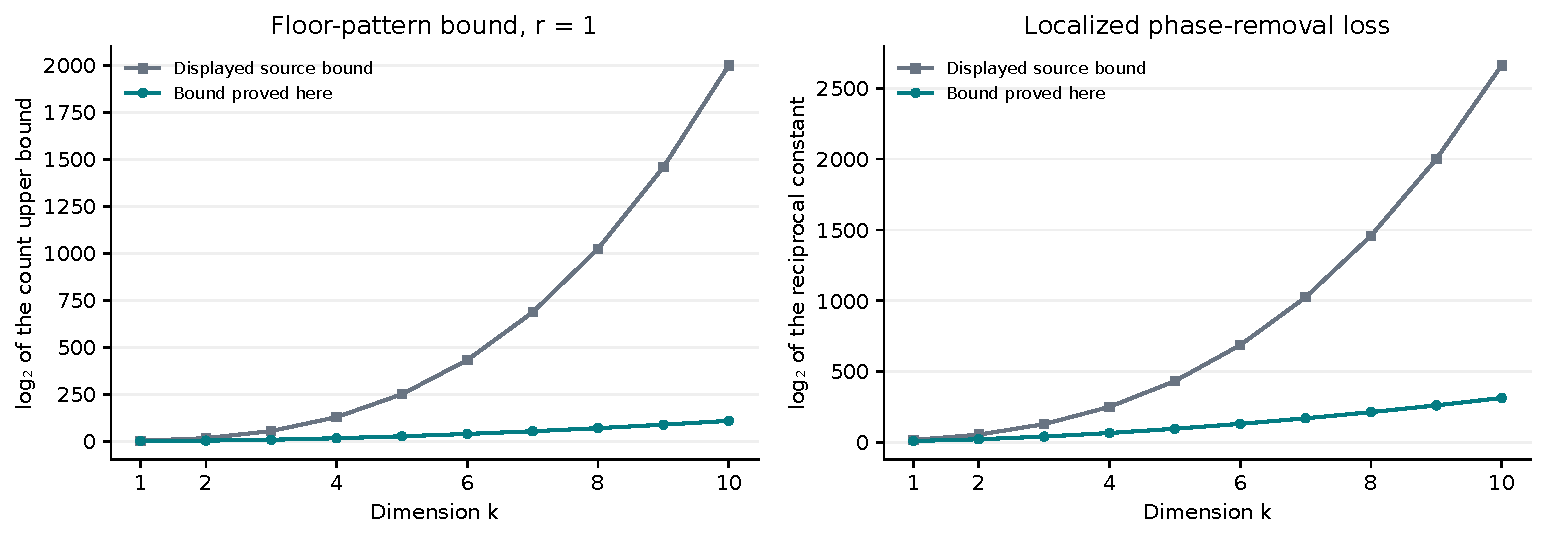
\includegraphics[width=\textwidth]{figures/06-carry-discrepancy-bound_comparisons.pdf}
 \caption{Comparison of logarithmic bounds. Lower values mean a smaller
 count upper bound (left) or a larger guaranteed local correlation
 constant (right). These are comparisons of local statements, not
 plots of final Szemer\'edi thresholds.}
 \label{gsr:fp:06:fig:comparison}
\end{figure}

For example, at $k=4,r=1$, the displayed floor-count exponent 128 is
replaced by the arrangement-based exponent approximately 15.650, and
the exact count is still smaller, namely $2^4C_4=2464$.
At $k=8$, the displayed local phase loss is $2^{-1458}$, whereas
\eqref{gsr:fp:06:eq:Kk} gives a constant approximately $2^{-212.704}$.
These comparisons quantify genuine local savings while leaving the
later structural dependencies explicit.

\gsroldfloats
\clearpage
\part{Lean interface, ledger crosswalk and research questions}\label{gsr:fz:part}
\partsource{
\textbf{Contents.} Sections~\ref{gsr:fz:sec:crosswalk} and~\ref{gsr:fz:sec:further} are the write's: the crosswalk of every comparison with the formal project, checked against the current ledger, and the deduplicated list of the sources' 46 research questions with credits (Vladimir's standing rule of 4~October 2026). Then each source's remaining sections, in source order: 01's formalization interface, questions, conclusions and appendices (delivered Sections~14--16, Appendices~A--B); 02's (Sections~10--12, Appendix~A); 03's iteration bookkeeping, Lean route, questions and reproducibility (Sections~9--11, Appendix~A); 04's quantitative comparisons, questions, closing perspective and appendices (Sections~9--11, Appendices~A--B); 05's Lean relation, computation, questions and conclusion (Sections~7--10). The sources' question sections are printed as delivered, with dated notes where another source answers a question.
}
\noindent\textbf{Reading conventions of this Part} (the full dictionary is Section~\ref{gsr:fm:sec:notation}).
\begin{center}\small
\begin{tabular}{@{}>{\raggedright\arraybackslash}p{0.17\textwidth} >{\raggedright\arraybackslash}p{0.78\textwidth}@{}}
\toprule
Symbol & Meanings in this Part, by source (\emph{tempting false reading} in italics)\\
\midrule
pins, counts & 01, 03: pin \texttt{3a25020a6}; 04, 05: pin \texttt{327773149}; 02: observed branch reference \texttt{66c02f8a1}. The ledger counts quoted by the sources (88 exact, 32 open) are those of the pins; at HEAD they are 98 and 22 (Section~\ref{gsr:fz:sec:crosswalk}).\\
Q$k$, (Q1), (Q2) & 04: its questions are numbered Q1--Q12 and two displays are tagged (Q1), (Q2); 01: numbered Questions (Section~\ref{gsr:fz:01:sec:questions}); 03: numbered Research questions (Section~\ref{gsr:fz:03:sec:research}); 02, 05: subsections and paragraphs. Item names in Section~\ref{gsr:fz:sec:further} are the write's.\\
\bottomrule
\end{tabular}
\end{center}
\medskip
\begingroup\small\noindent\textbf{Added in the second write (6~October 2026): sources 06--10.} \textbf{Contents.} The write's Sections~\ref{gsr:fz:sec:crosswalk} and~\ref{gsr:fz:sec:further} are extended by dated additions: the crosswalk to the ledger at HEAD of this write, and the 50 research questions of sources 06--10 (plus two inline question paragraphs of source~10) merged into the theme lists. Then the remaining sections of the new sources, in source order: 06's iteration potential, Lean map and questions (delivered Sections~6, 8, 9); 07's verification, questions, conclusion and reproduction commands (Sections~9--11, Appendix~B); 08's Lean integration, checks, questions, conclusion and build provenance (Sections~11--14, Appendix~B); 09's checks, Lean integration, questions, conclusion and dependency map (Sections~11, 12, 14, 15, Appendix~C); 10's iteration bookkeeping, Lean map, questions and provenance (Sections~10--12, Appendix~A).\par\endgroup
\medskip
\noindent\textbf{Reading conventions for the sections of sources 06--10 in this Part.}
\begin{center}\small
\begin{tabular}{@{}>{\raggedright\arraybackslash}p{0.17\textwidth} >{\raggedright\arraybackslash}p{0.78\textwidth}@{}}
\toprule
Symbol & Meanings in this Part, by source (\emph{tempting false reading} in italics)\\
\midrule
pins, counts (06--10) & 06, 09, 10: pin \texttt{7d99e5dee}; 07: pin \texttt{ae0e89574}; 08: no commit, blob identifiers of \texttt{7d99e5dee}. The ledger counts quoted by 06 and~10 (95 exact, 25 open) and 06's ``140 modules, 1,365 theorems'' are those of \texttt{7d99e5dee}; at HEAD \texttt{764740f07} they are 99 and 21, and \file{FORMALIZATION_STATUS.txt} reports 196 modules and 1,805 audited theorems (Section~\ref{gsr:fz:sec:crosswalk}).\\
iteration & 06: $F$, $G$ the increment and the charge of Lemma~\ref{gsr:fz:06:iter:potential}, $c,p,q,a_0$ the local rule, $A=\log(1/a_0)$, $L=\log(1/\delta_0)$, $B(\delta_0)$ the double-logarithmic budget. 10: $c$, $a$ the increment rule, $\vartheta_i$, $b_i$ the length rule, $P_t$, $M_t$. \emph{06's $L$ is a logarithm, not a length; $p$ is an exponent, not a prime.}\\
\bottomrule
\end{tabular}
\end{center}
\medskip
\section{The formal project: ledger crosswalk \wtag}\label{gsr:fz:sec:crosswalk}
\par\noindent{\small\textit{Added in the write, 6~October 2026.}}\par
Every comparison that a source makes with a corrected statement of the formal project was checked against the ledger and the Lean declarations at HEAD \texttt{25df8755d} (6~October 2026). File and line numbers below are at that commit. Statements are \file{Sections*.lean} propositions; ``exact'' means the ledger lists an exact companion theorem. The ledger then records 98 exact companions and 22 open statements; at all three pins it recorded 88 and 32. The last column gives the formal status of the \emph{improvement}. All of the comparisons are accurate at HEAD, except the stale ones the table names.

\begingroup\small
\renewcommand{\theHtable}{crosswalk.\arabic{table}}
\begin{longtable}{@{}>{\raggedright\arraybackslash}p{0.12\textwidth} >{\raggedright\arraybackslash}p{0.32\textwidth} >{\raggedright\arraybackslash}p{0.26\textwidth} >{\raggedright\arraybackslash}p{0.21\textwidth}@{}}
\toprule
Gowers & Lean statement; companion (status) & Source claim here & Improvement\\
\midrule
\endhead
Lemma 2.3 & \file{lemma_2_3} (\file{Sections01\_03}:141); \file{lemma_2_3_holds} (\file{Proofs02Partition}:561) (exact) & constant $1/4\to1/3$, optimal under the Lean hypotheses (05, Thm.~\ref{gsr:dt:05:thm:sharp-capped}) & not formalized\\
Cor.~2.4 & \file{corollary_2_4} (:158); \file{corollary_2_4_holds} (\file{Proofs02PhasePartition}:276); also \file{corollary_2_4_before_rounding_repair_false} (exact) & $128\pi\to36\pi$, $\alpha/2\to3\alpha/4$, same upper length, $r\le N$ dropped (05, Cor.~\ref{gsr:dt:05:cor:cor24}) & not formalized\\
Cor.~2.5 & \file{corollary_2_5} (:180); \file{corollary_2_5_holds} (\file{Proofs02DensityIncrement}:517); proof-level pair $\sqrt{\alpha N/128\pi}$, $\alpha/4$ in private \file{cor25_large_scale} (:375) (exact) & density-sensitive increments (01, 03, 05); 03 and 05 compare with the proof-level pair, 01 with the statement (note after Table~\ref{gsr:dt:01:tab:increment}) & not formalized\\
Thm.~3.2, Cor.~3.3 & \file{theorem_3_2_holds} (\file{Proofs03ProgressionAverage}:381); \file{corollary_3_3} (:276), \file{corollary_3_3_holds} (\file{Proofs03ProgressionCount}:349) (exact; $N$ prime, $k\le N$) & $2^k\alpha\to(k-2)\alpha$ in normalized terms; admissible slopes (03, 04, Part~III) & not formalized\\
Cor.~3.6 & \file{corollary_3_6} (:310); \file{corollary_3_6_holds} (\file{Proofs03ProgressionExistence}:157) (exact) & density exponent $k2^{k-1}$ against $k2^k$ (04, Cor.~\ref{gsr:cc:04:prog:super}) & not formalized\\
Lemma 3.8 & \file{lemma_3_8_holds} (\file{Proofs03GowersCS}:513); \file{gowers_cauchy_schwarz} (:485); \file{gowersNorm_add_le} (\file{Proofs03Minkowski}:131) (exact) & used as tools (03, 04) & ---\\
Lemma 3.10 & \file{lemma_3_10} (:340); \file{lemma_3_10_holds} (\file{Proofs03CubeUpper}:82) (exact) & excess $\alpha^{1/2^d}\to\alpha^{4/2^d}$ (03); leading $6\sqrt2\,\delta^4u^4$ for $d=3$ (04) & not formalized\\
Cor.~5.6 & \file{corollary_5_6} (\file{Section05}:205); \file{corollary_5_6_holds} (\file{Proofs05FullPartition}:85) (\textbf{exact at HEAD, open at every pin}) & 02 imports it as $\mathrm{PP}(K,R_0)$ with the same constants; \emph{02's ``not Lean-verified'' is stale} (note in Section~\ref{gsr:dt:02:sec:refinement}) & 02's Thm.~\ref{gsr:dt:02:thm:refine} not formalized\\
Cor.~5.8 & \file{corollary_5_8} (\file{Section05}:242) (open); \file{corollary_5_8_with_scale_holds} (\file{Proofs05FullPartition}:94) proves a scale-qualified repair & 02 declines to restate it (Section~\ref{gsr:dt:02:sec:d8}) & ---\\
Lemma 5.15 & \file{lemma_5_15} (\file{Section05}:352); \file{lemma_5_15_holds} (\file{Proofs05\_10}:735) (exact; $\alpha\ge0$, empty cells allowed) & size $\alpha N/(4M)\to\alpha(2+\alpha)N/(2(4-\alpha)(M-1))$ for $\alpha>0$, nonempty cells (02, 03) & not formalized\\
Prop.~6.1 & \file{proposition_6_1} (\file{Sections06\_07}:37); \file{proposition_6_1_holds} (\file{Proofs05\_10}:505) (exact) & recovered by 02's Thm.~\ref{gsr:en:02:thm:main} with $m(f)\le1$, $\U\le m^4$ & not formalized\\
Prop.~7.3 & \file{proposition_7_3} (:135); \file{proposition_7_3_holds} (\file{Proofs07BalogSzemeredi}:996); also \file{proposition_7_3_group_holds} (exact) & $(2^{-20}c^{12},2^{38}c^{-24})\to(c/8,2^{19}c^{-9})$ (03) & not formalized\\
Lemma 7.4 & \file{lemma_7_4} (:167); \file{lemma_7_4_holds} (\file{Proofs07DRC}:536), five witnesses (exact) & $2^{-1/2}\delta^5n\to7\delta^3n/(3\sqrt6)$ (03) & not formalized\\
Lemma 9.2 & \file{lemma_9_2} (\file{Sections08\_09}:69); \file{lemma_9_2_holds} (\file{Proofs09Moments}:527); exact $N^2|B|$ at line~495 (exact) & (M4) exact Parseval is proof-level; (M5) $\gamma^7\beta^{15}p^{15}$ (04) & not formalized\\
Lemma 9.3, Cor.~9.4 & \file{lemma_9_3} (:77), \file{corollary_9_4} (:91); companions \file{Proofs09Restriction}:376, :416 (exact; \emph{no primality}) & prime-field restriction, $2^{-95}\gamma^{112}\eta^{15}|B|^{15}$ (04); does not prove the Lean statements, as 04 says & not formalized\\
Lemma 12.4 & \file{lemma_12_4} (\file{Sections12\_13}:158); \file{lemma_12_4_holds} (\file{Proofs12Amplification}:21) (exact) & $\beta^{112}\to\beta^{106}$ (04, (A12)) & not formalized\\
Cor.~14.6, Lemmas 14.7, 14.8 & \file{corollary_14_6} (\file{Sections14\_15}:266), \file{lemma_14_7} (:279), \file{lemma_14_8} (:292); companions \file{Proofs14Arrangements}:838, \file{Proofs14HigherArrangements}:712, \file{Proofs14ProductToArrangements}:18 (exact) & profile $\sigma$; $7\cdot4^{k+1}\to7\cdot4^{k+1}-6$ (04, Thm.~\ref{gsr:en:04:mom:arrangements}) & not formalized\\
Lemma 17.4, Cors.~17.5, 17.6 & \file{lemma_17_4_holds} (\file{Proofs17Regions}:691); \file{corollary_17_5} (\file{Sections17\_18}:103), \file{corollary_17_6} (:117); companions \file{Proofs17FinitePatterns}:396, :501 (exact) & $2^{2rk^3}\to(2r)^kC_k$; $M2^{2r(k+1)^3}\to M\min(2r,M)^kR_{k+1}(k2^{k-1})$ (01, 04, Part~IV) & not formalized\\
Prop.~17.7 & \file{proposition_17_7} (:140); \file{proposition_17_7_holds} (\file{Proofs17LocalizedPhaseRemoval}:2900), joint \texttt{hyperplaneRegionCount} (exact) & $2^{-2(k+1)^3}\to2^{-k^2-k\log_2k-O(k)}$ (04); weaker interface (01) & not formalized\\
Cor.~16.11, Thms.~1.3, 18.1, 18.2 & all \textbf{open}; \file{theorem_18_1}'s docstring warns about the tower estimate of Cor.~16.11 & 01's dependency warning (Section~\ref{gsr:fz:01:sec:formal}) & ---\\
Section 18 (interval transfer) & \file{hasNatAP_of_short_modular_sequence} (\file{Proofs18IntervalTransfer}:22), \file{hasNatAP_of_hasModAP_image} (:92), added in \texttt{327773149} & 04's Lemma~\ref{gsr:cc:04:prog:lift}; 03's Remark~\ref{gsr:cc:03:rem:rectify} & \textbf{formalized} (same statement, $n-1\mapsto n$)\\
\bottomrule
\end{longtable}
\endgroup

\emph{Normalizations.} The Lean development uses the unnormalized Fourier transform and the unnormalized Gowers norm; the intake found the sources' conversion tables accurate (source~02's Section~\ref{gsr:fz:02:sec:formal} and Appendix, source~03's Section~\ref{gsr:fz:03:sec:formal}); the write did not re-derive them. \file{Definitions.lean} has changed since the pins only by an added \texttt{Box.IsProper}, which no source uses; every other file that a source cites is unchanged.

\emph{Formal status of this report.} As stated in Section~\ref{gsr:fm:sec:formal}: the lifting lemma is formalized and was formalized before the sources arrived; nothing else here is. The reciprocal pointer for \file{Combinatorics/Ramsey/FORMALIZATION\_STATUS.txt} is left to the session that maintains the Lean development.

\begin{writenote}[6 October 2026; sources 06--10]
\emph{The ledger at the second write.} At HEAD \texttt{764740f07} (6~October 2026) the ledger records 99 exact companions and 21 open statements, and \file{FORMALIZATION\_STATUS.txt} reports 196 modules reachable from the audit and 1,805 audited public theorems. Since the first write's HEAD \texttt{25df8755d} the statements closed are: \file{lemma_16_9}. Since \texttt{7d99e5dee}, the pin of sources~06, 09 and~10 (95 exact, 25 open, 140 modules, 1,365 theorems), 4 statements have closed: \file{lemma_16_1}, \file{lemma_16_5}, \file{lemma_16_6} and \file{lemma_16_9}; since \texttt{ae0e89574}, the pin of source~07, 4: \file{lemma_16_1}, \file{lemma_16_5}, \file{lemma_16_6} and \file{lemma_16_9}. The table above keeps its file and line numbers at \texttt{25df8755d}; the rows below give them at \texttt{764740f07}. The Lean development is being extended by another session as this is written, so the counts may already have moved. Every comparison made by sources~06--10 with a formal statement was checked against these declarations and is accurate, except the stale counts corrected in the notes after source~06's Section~\ref{gsr:fm:06:sec:d1} and source~10's Section~\ref{gsr:fm:10:sec:d1}.
\end{writenote}

\begingroup\small
\renewcommand{\theHtable}{crosswalk2.\arabic{table}}
\begin{longtable}{@{}>{\raggedright\arraybackslash}p{0.12\textwidth} >{\raggedright\arraybackslash}p{0.32\textwidth} >{\raggedright\arraybackslash}p{0.26\textwidth} >{\raggedright\arraybackslash}p{0.21\textwidth}@{}}
\toprule
Gowers & Lean statement; companion (status) & Claim of sources 06--10 & Improvement\\
\midrule
\endhead
Cor.~2.5 & \file{corollary_2_5} (\file{Sections01\_03}:180); \file{corollary_2_5_holds} (\file{Proofs02DensityIncrement}:517) (exact) & increment $\delta\eta/(4\delta-\eta)$ at source~01's length; the frontier $D_\gamma$, $L_\gamma$ (10, Thm.~\ref{gsr:dt:10:thm:frontier}) & not formalized\\
Thm.~2.6 & \file{theorem_2_6} (:189); \file{theorem_2_6_holds} (\file{Proofs02Roth}:1238) (exact) & step count $321(\delta_0^{-1}-1)$ against the transcription's $640\delta_0^{-1}$ (10, Prop.~\ref{gsr:fz:10:prop:iteration}) & not formalized\\
Thm.~3.2, Cors.~3.3, 3.6 & \file{theorem_3_2_holds} (\file{Proofs03ProgressionAverage}:381); \file{corollary_3_3} (:276), \file{corollary_3_3_holds} (\file{Proofs03ProgressionCount}:349); \file{corollary_3_6} (:310), \file{corollary_3_6_holds} (\file{Proofs03ProgressionExistence}:157) (exact) & two-target bound and quadratic discrepancy, $\alpha\le(\delta^{k-1/2}/2B_k)^{2^{k-2}}$ (06); torsion kernels, error $\delta S_k\eta$, $\alpha\le(\delta^{k-1}/2S_k)^{2^{k-1}}$ (10) & not formalized\\
Lemmas 3.7, 3.10 & \file{lemma_3_7} (:320), \file{lemma_3_7_holds} (\file{Proofs03Cubes}:184); \file{lemma_3_10} (:340), \file{lemma_3_10_holds} (\file{Proofs03CubeUpper}:82) (exact) & excess of fourth order with exact quartic term (08, 09) and quintic term (09); exponent $4/2^d$ sharp for sets; lower bound $(\delta^4+E_4)^{2^d/4}$ (08) & not formalized\\
Lemma 5.15 & \file{lemma_5_15} (\file{Section05}:352); \file{lemma_5_15_holds} (\file{Proofs05\_10}:735) (exact) & fixed-$M$ optimum, $\tau(\alpha)$ (06); cap and tail (10) & not formalized\\
Prop.~7.3 & \file{proposition_7_3} (\file{Sections06\_07}:135); \file{proposition_7_3_holds} (\file{Proofs07BalogSzemeredi}:996) (exact) & $(c/4,\,2^{10}c^{-5})$ on any abelian group (10) & not formalized\\
Lemma 7.5, Cor.~7.6 & \file{lemma_7_5} (:183), \file{lemma_7_5_holds} (\file{Proofs07FreimanRestriction}:267); \file{corollary_7_6} (:197), \file{corollary_7_6_holds} (\file{Proofs07AdditiveRestriction}:100) (exact) & $|B|/(k(h_k-1)+1)$; $2^{-209}\gamma^{103}$ against $2^{-1882}\gamma^{1164}$ (10); both imply the formal conclusions (note after Cor.~\ref{gsr:en:10:cor:improved-order-eight}) & not formalized\\
Lemma 10.9 & \file{lemma_10_9} (\file{Section10}:335); \file{lemma_10_9_holds} (\file{Proofs10Shift}:717) (exact; \texttt{FreimanHom 2}) & order five under exactly these hypotheses; order nine with the hypotheses of \file{lemma_10_6} and the set-up (07) & not formalized; order nine needs a new statement\\
Cors.~17.5, 17.6 & as in the table above (\file{Sections17\_18}:103, :117; \file{Proofs17FinitePatterns}:396, :501) (exact) & $(2r)^kC_k$, $\min(2r,M)^kC_{k,M}$, entropy uniform in $M$; $C_4=154$ certified (06) & not formalized\\
Prop.~17.7 & \file{proposition_17_7} (:140); \file{proposition_17_7_holds} (\file{Proofs17LocalizedPhaseRemoval}:2900) (exact) & $1/(8K_k^2)=2^{-2k^2-O(k\log k)}$ (06) & not formalized\\
Cor.~16.11, Thms.~18.1, 18.2 & \file{corollary_16_11} (\file{Section16}:893), \file{theorem_18_1} (\file{Sections17\_18}:171), \file{theorem_18_2} (:190): \textbf{open}; \file{section18_cyclic_density_increment_holds_of_theorem_18_1} (\file{Proofs18QuantitativeSzemeredi}:169) & dependency warnings (06, 10); iteration potential (06) & ---\\
\bottomrule
\end{longtable}
\addtocounter{table}{-1}% uncaptioned: keeps the table numbers of sources 01--05
\endgroup

\begin{writenote}[6 October 2026; sources 06--10]
\emph{Formal status after the second write.} No statement of sources~06--10 is formalized, and none gains formal status by its placement. The only formalized statement of the report is still the lifting lemma of source~04. Sources~06--10 ship no Lean files; their formalization plans are in Part~V (source~07's also as \file{07-transport-rigidity-FORMALIZATION.md}).
\end{writenote}
\section{Further questions and research \wtag}\label{gsr:fz:sec:further}
\par\noindent{\small\textit{Added in the write, 6~October 2026.}}\par
This section applies Vladimir's standing rule of 4~October 2026: no unproved or wrong claim is dropped; open claims are stated as questions with their source, the argument they came with and what is missing; wrong claims stay on record with a proof of their failure. The five sources ask 46 questions: source~01 ten (Section~\ref{gsr:fz:01:sec:questions}, Questions~1--10 there in order), source~02 seven (Section~\ref{gsr:fz:02:sec:questions}, delivered Subsections~11.1--11.7), source~03 nine (Section~\ref{gsr:fz:03:sec:research}, Research questions~1--9 there in order), source~04 twelve (Section~\ref{gsr:fz:04:sec:research}, Q1--Q12) and source~05 eight (Section~\ref{gsr:fz:05:sec:questions}, paragraphs~1--8). They are printed there as delivered. Below they are grouped by theme, with every asking source credited; the counts per theme are 14, 9, 8, 7 and 8. Items are numbered within their theme, so later additions extend a list without renumbering it.

\begin{writenote}[6 October 2026; sources 06--10]
\emph{Sources 06--10.} They ask 50 further numbered questions: source~06 eleven (Section~\ref{gsr:fz:06:sec:research}, Questions~1--11 there), source~07 eight (Section~\ref{gsr:fz:07:sec:questions}, Questions~1--8 there in order), source~08 ten (Section~\ref{gsr:fz:08:sec:questions}, Questions~1--10 there in order), source~09 ten (Section~\ref{gsr:fz:09:sec:questions}, Research questions~1--10, its Subsections~14.1--14.10) and source~10 eleven (Section~\ref{gsr:fz:10:sec:research}, items~1--11 there). Source~10 also ends its Sections~\ref{gsr:cc:10:sec:d6} and~\ref{gsr:en:10:sec:d8} with a paragraph of questions; both are credited below. The intake dossier counted ten questions for source~10 and 95 in all; the count is 96. They are added to the themes below as new items or, where they ask the same thing, merged into an existing item by a dated sentence. The counts per theme become 17, 19, 33, 13 and~14 (the headings below keep the counts of sources~01--05).

\emph{Unproved or wrong claims in sources 06--10.} The intake and the second write found no claim of sources~06--10 that is wrong, and no claim asserted as proved without a proof. One wrong statement is on record: the quartic lower bound with coefficient~$12$, which sources~08 and~09 pose and refute themselves and source~03 also refutes; Remark~\ref{gsr:cc:rem:falselower} keeps it with an explicit counterexample. Inputs used but not proved in the sources: Zuev's threshold-function count (source~06, as for source~01), the Pl\"unnecke--Ruzsa inequality (source~10, via Petridis) and, for source~10's labelled modern-input variant only, the Reiher--Schoen theorem; these are published theorems. Source~10's ``independent review'' is not shipped, and nothing rests on it. Statements of the intake corrected at the write: source~06's improvement over the $M-1$ corollary is strict only for $\alpha<1$ (note after Corollary~\ref{gsr:dt:02:cor:515}); source~01's increment dominates source~10's by $3/2$ only for $\gamma\le1/2$ (note after Table~\ref{gsr:dt:01:tab:increment}); source~09's date for version~2 of Shi--Dong is wrong (bibliography).

\emph{Answered or advanced inside the report.} Source~08's question whether $\kappa_3^{\mathrm{odd}}=1/\sqrt2$ is answered yes by source~04 (item~\ref{gsr:fz:q:III:normgap}). Source~03's question on the fifth coefficient is answered by source~09 (item~\ref{gsr:fz:q:III:fifth}). Source~02's finite-cell problem is solved in the weighted model by source~06 (item~\ref{gsr:fz:q:I:finitecell}). Source~04's Question~8 is answered a second time by source~06 (item~\ref{gsr:fz:q:IV:second}). Source~06's Question~7 is advanced by source~10 for one distinguished function (item~\ref{gsr:fz:q:III:torsion}). Source~04's Question~10 (non-admissible slopes) is advanced by source~10's torsion factors (item~\ref{gsr:fz:q:III:mixed}).
\end{writenote}

\emph{Unproved or wrong claims.} The intake and the write found no claim of sources~01--05 that is wrong, and no claim asserted as proved without a proof. Three inputs are used but not proved in the sources. The classical threshold-function counts (Zuev; Kahn--Koml\'os--Szemer\'edi; Baldi--Vershynin) enter source~01's asymptotics and are published theorems. The partition input $\mathrm{PP}(K,R_0)$ of source~02 is now a formal theorem for polynomial phases on intervals (Section~\ref{gsr:fz:sec:crosswalk}). The ``independent mathematical reviews'' of source~03 are not shipped, and nothing here rests on them. Two values found at intake are not certified, $C_5=8410$ and $A_4=770$; they are item~\ref{gsr:fz:q:IV:counts}.

\emph{Answered inside the report} (dated notes at the questions). Source~04's Question~8, the leading constant of $\log_2F_k/k^2$ and $\log_2A_k/k^2$, is answered by source~01: it is $1$, using the classical threshold count, and source~01 certifies $F_4=C_4=154$. Source~03's Research question on $c_d^{\mathrm{odd}}$ is answered for $d=3$ by source~04's Theorem~\ref{gsr:cc:04:cub:norm-gap}: $c_3^{\mathrm{odd}}=2^{-1/2}$, attained by real parts of characters. With it, source~03's Remark~\ref{gsr:cc:03:cube:sharpremark} is settled at $d=3$. Source~04's Question~3 is the same question as source~03's for $d\ge4$, and is merged with it (item~\ref{gsr:fz:q:III:normgap}).

\subsection*{Theme I: density transfer and phase-flat partitions (14 questions)}
\begin{enumerate}[label=\textbf{I.\arabic*},ref=I.\arabic*,leftmargin=2.6em]
\item\label{gsr:fz:q:I:higher} \emph{Higher-degree phase partitions} (01 Question~8; 05 paragraph~6). The density transfer is proved for any short-arc phase (source~01's Theorem~\ref{gsr:dt:01:thm:tail}; source~05's Proposition~\ref{gsr:dt:05:prop:transfer} and Corollary~\ref{gsr:dt:05:cor:gram}). Missing: polynomial or nilsequence partitions with a quantitative minimum cell length and small occupied exceptional mass (01), and density-sensitive oscillation budgets tracked through geometric complexity with all losses parameterized (05). Simultaneous linear approximation does not give them, and Theorem~\ref{gsr:dt:05:thm:minimax} does not transfer to nonlinear phases.
\item\label{gsr:fz:q:I:arith} \emph{The best transfer under arithmetic constraints} (01 Question~5; 05 paragraph~4). The extremizers of Theorem~\ref{gsr:dt:01:thm:tail} rotate cell arcs freely, and the disk radius and the capacity inequality are separately sharp (05). Asked: how much stronger the tail becomes for one fixed cyclic character on a common-step partition with nearly equal cells (01), and the exact feasible region of block positive mass, correlation, density and phase width (05).
\item\label{gsr:fz:q:I:profile} \emph{Finite partition profiles and the size--increment trade-off} (05 paragraph~1; 01 Question~6). The universal constant $1/3$ is settled (Theorem~\ref{gsr:dt:05:thm:sharp-capped}). Asked: the exact best minimum length for each $(r,s,M)$ and slope, and the feasible pairs of minimum and maximum lengths (05); the best uniform pair of length and increment, combining \eqref{gsr:dt:01:eq:pareto} with an optimal finite partition, including the final incomplete blocks (01). \emph{[6~October 2026; sources 06--10]} Source~10 (its Question~3) asks the same for its phase partition: the best universal minimum block length for a prescribed phase-disc radius with all integer rounding retained, first at fixed $\eta/\delta$ as $\delta\to0$; its density cap is sharp, its passage from one approximate period to blocks of lengths $L,\ldots,2L-1$ may not be.
\item\label{gsr:fz:q:I:moments} \emph{Retaining more than one density statistic} (01 Question~7). Theorem~\ref{gsr:dt:01:thm:knots} solves the optimization once stop-loss statistics are chosen. Missing: structural lemmas that propagate those statistics through repeated localization at acceptable cost.
\item\label{gsr:fz:q:I:budget} \emph{Heterogeneous phase budgets} (02 Subsection~11.5; 03 Research question~5). The analytic constraint is exact (source~02's heterogeneous inequality in Section~\ref{gsr:dt:02:sec:phase}; source~03's Lemma~\ref{gsr:dt:03:selection:phase}). Missing: a refinement theorem whose cost depends on the oscillation allowed in each cell, so that budgets can be allocated by local mass. Any better $\mathrm{PP}(K,R_0)$ transfers automatically to Theorem~\ref{gsr:dt:02:thm:refine}.
\item\label{gsr:fz:q:I:finitecell} \emph{The finite-cell extremal problem} (02 Subsection~11.6). Theorem~\ref{gsr:dt:02:thm:tail} solves the weighted total-mass problem. Open: the largest good cell when $M$ and the allowed cell sizes are fixed, with integer cardinalities, which would sharpen the $M-1$ corollary. \emph{[6~October 2026; sources 06--10]} \emph{Advanced by source~06:} with $M$ fixed and the cell masses free, its Theorem~\ref{gsr:dt:06:den:sharp} gives the exact optimum $\min\{P_+/(b(M-1)),S/(M-2)\}$ with explicit extremizers (note after Corollary~\ref{gsr:dt:02:cor:515}). Still open: prescribed allowed cell sizes and integer cardinalities at a fixed $N$.
\item\label{gsr:fz:q:I:minimax} \emph{Constants in the simultaneous minimax theorem} (05 paragraph~2). The exponent $1/(m+1)$ and the dependence on $\varepsilon$ are sharp; the upper constant $c_m$ is poor. Asked: the optimal leading constants, first for one or two phases (source~01's Theorem~\ref{gsr:dt:01:thm:barrier} improves the one-phase constant), the effect of a common difference, and the order of limits.
\item\label{gsr:fz:q:I:aniso} \emph{Anisotropic lower bounds} (05 paragraph~3). Is there a matching minimax upper bound in all anisotropic regimes, with the regime decomposition that loose tolerances require?
\item\label{gsr:fz:q:I:adaptive} \emph{Adaptive selection of frequencies and tolerances} (05 paragraph~5). Proposition~\ref{gsr:dt:05:prop:waterfill} solves the continuous allocation. Missing: subset selection and the exact ceiling problem, relative to certified Fourier inputs.
\item\label{gsr:fz:q:I:interval} \emph{Interval-localized spectral extraction} (05 paragraph~8). Corollary~\ref{gsr:dt:05:cor:gram} corrects for the Gram matrix by its top eigenvalue only. Missing: certified conditioning bounds for specific frequency configurations, using more of the Gram matrix. \emph{[6~October 2026; sources 06--10]} Source~10 (its Question~4) asks the companion problem: when several approximately constant characters or polynomial phases live on one partition, the best Gram-matrix lower bound for the conditional second moment, to be combined with its variance cap \eqref{gsr:dt:10:eq:variance-cap}; the common partition has to be supplied by the geometry, not assumed.
\item[] \textit{Added in the second write, 6~October 2026 (sources 06--10):}
\item\label{gsr:fz:q:I:densecells} \emph{Using the mass of all dense cells} (06 Question~8). Source~06's Theorem~\ref{gsr:dt:06:den:sharp} controls the total mass above every threshold, not only one cell, and its extremizers show that the scalar data cannot give more. Asked: whether a branching density-increment argument, keeping geometric information about the collection of high cells, improves a structural or counting bound. Related to item~\ref{gsr:fz:q:I:moments}.
\end{enumerate}
The ten items carry the fourteen questions: 01 Questions~5--8, 02 Subsections~11.5--11.6, 03 Research question~5, and 05 paragraphs~1--6 and~8.
\emph{[6~October 2026; sources 06--10]} With sources~06--10 the eleven items carry seventeen questions: also 06 Question~8 and 10 Questions~3--4.

\subsection*{Theme II: the inverse step (9 questions)}
\begin{enumerate}[label=\textbf{II.\arabic*},ref=II.\arabic*,leftmargin=2.6em]
\item\label{gsr:fz:q:II:structure} \emph{A correlation-preserving structural theorem for multivalued spectra} (02 Subsection~11.1). Proposition~\ref{gsr:en:02:prop:spectrum} keeps all large derivative frequencies. Missing: an energy-to-structure step that keeps a fixed fraction of $t_\tau$ and exploits $\kappa$, controlling both losses.
\item\label{gsr:fz:q:II:near} \emph{Near equality for the coupled pair $(f,w)$} (02 Subsection~11.2). Proposition~\ref{gsr:en:02:prop:stability} gives two alignments, and the equality examples show distinct geometries. Asked: a dimension-free description of $f$ and $w$ jointly when Theorem~\ref{gsr:en:02:thm:main} is nearly an equality; results on near-maximal Gowers norms (Eisner--Tao) are relevant but do not classify the weight.
\item\label{gsr:fz:q:II:profiles} \emph{Carrying profiles through the proof} (02 Subsection~11.3; 04 Q7). Keep the distribution of $m(\Delta_{\mathbf h}f)$ and $\U(\Delta_{\mathbf h}f)$ across slices instead of their supremum (02), and the cross-section profile $\sigma=\E_r\beta_r^3$ through later restrictions (04). The difficulty in both: compatibility of structure between slices, and which operations preserve the profile.
\item\label{gsr:fz:q:II:drc} \emph{The sharp fixed-threshold DRC profile} (03 Research question~3). The order of the best guaranteed $|K|/n$ under Lemma~7.4's exact criterion as $\delta\to0$, and whether the exponent $3$ of Theorem~\ref{gsr:en:03:drc:cubic-selection} can be improved using constraints of actual intersection matrices; the scalar argument only rules out a two-witness first-moment certificate.
\item\label{gsr:fz:q:II:extraction} \emph{Optimizing the elementary extraction} (03 Research question~4). Optimize $\gamma,\varepsilon,\beta$, walk lengths and popularity thresholds in Proposition~\ref{gsr:en:03:drc:graph-compression}, judging the pair of conclusions together and keeping the comparison with Reiher--Schoen explicit.
\item\label{gsr:fz:q:II:threshold} \emph{Lowering the size threshold of the restriction theorem} (04 Q4), from $|B|\ge\Lambda_d(\alpha\eta)^{-2d}$, by reflecting the additive structure of $B$ in the exceptional relations or by a better kernel, with repeated entries handled.
\item\label{gsr:fz:q:II:retention} \emph{The optimal retention law} (04 Q5). Proposition~\ref{gsr:en:04:rest:method-bound} limits one expectation budget only. Asked: upper-bound examples or a better selection method, and simultaneous guarantees on $|B'|$, its energies and the respected density.
\item\label{gsr:fz:q:II:groups} \emph{Restriction beyond prime cyclic groups} (04 Q6): versions for $\Z/N\Z$, $\F_q^n$ and other codomains, with hypotheses that quantify kernels of the coefficient maps.
\item[] \textit{Added in the second write, 6~October 2026 (sources 06--10):}
\item\label{gsr:fz:q:II:nonuniform} \emph{The optimal nonuniform transport threshold} (07 Question~1). For fixed $k\ge2$ and fibre ratio $\kappa>1$, the largest universal $\delta$ forcing order-$k$ relations, and the gain from a separate boundary bound. Proved: $1/(2[1+(k-1)\kappa])$ (Corollary~\ref{gsr:en:07:cor:freiman}); sharp only at $\kappa=1$ (Theorem~\ref{gsr:en:07:thm:sharp}). Suggested: a finite search over fibre sizes and actual value assignments, not independent error profiles.
\item\label{gsr:fz:q:II:order} \emph{The largest guaranteed Freiman order at Lemma~10.9} (07 Question~2), under the exact Lean hypotheses (order five proved) and under the ambient package (order nine proved). Five and nine are lower bounds; counterexamples must satisfy the nested local model, not only a scalar defect bound.
\item\label{gsr:fz:q:II:winding} \emph{Stability of winding obstructions} (07 Question~3): must a violated relation with total budget close to one come from a few cuts or carry boundaries, after a structural reduction?
\item\label{gsr:fz:q:II:certificates} \emph{Efficient certificates for many relations} (07 Question~4): compressing the root-law linear programs of Theorem~\ref{gsr:en:07:thm:lp} over a large family of relations, for instance by translation symmetry or a presentation of the generated group; one relation is a finite linear program, exponentially many are not efficient.
\item\label{gsr:fz:q:II:jointext} \emph{Joint optimization of extraction and transport} (07 Question~5): building the regular component and its source law together, so that the domain is large and the relevant profiles small, accounting for lost cardinality and the relation between energy weights and the chosen law.
\item\label{gsr:fz:q:II:coherence} \emph{Higher-dimensional coherence} (07 Question~6): shared-vertex sampling on cubes or other diagrams in place of nested exceptional sets in bilinear and multilinear exactification; the joint law must be specified first and every marginal proved.
\item\label{gsr:fz:q:II:extraction5} \emph{The earlier exponent $\eta^{1/5}$} (07 Question~7): which losses before the local model are necessary, and whether the fifth root can be improved while keeping a large regular component and direction set. Source~07 removes the later square root only.
\item\label{gsr:fz:q:II:fibre} \emph{A sharp vertical-fibre restriction theorem} (10 Question~5 and the question paragraph at the end of Section~\ref{gsr:en:10:sec:d8}). How close is $|B|/(k(h_k-1)+1)$ to the best bound determined by the defect fibre alone; can the factor $k$ be reduced under additive structure of $H_k$; can $|H_k|$ be bounded from a vertical energy profile, how does it grow with $k$, and when does an order-$k$ homomorphism extend to order $k+1$ with small loss? Settled only for $H_k=\{0\}$.
\item\label{gsr:fz:q:II:badstep} \emph{Overlaps in the bad-step union} (10 Question~6): Theorem~\ref{gsr:en:10:thm:torsion-fibre-extraction} uses a union bound over $E_j=\{d\ne0:jd\in F\}$; an exact treatment of their intersections, for example for cyclic prime-power codomains via valuations, would improve the general-codomain retention.
\item\label{gsr:fz:q:II:energyprop} \emph{Propagating a modern energy input} (10 Question~7): propagate the Reiher--Schoen retention (almost $\sqrt\gamma$, against $\gamma/4$ here) with the exact vertical fibre through the later Bohr-neighbourhood and local-linearity stages, producing a complete chain of inequalities rather than an isolated replacement of the exponent $1164$. Related to item~\ref{gsr:fz:q:II:extraction}.
\end{enumerate}
The eight items carry the nine questions: 02 Subsections~11.1--11.3, 03 Research questions~3--4, and 04 Q4--Q7.
\emph{[6~October 2026; sources 06--10]} With sources~06--10 the eighteen items carry nineteen questions and one question paragraph: also 07 Questions~1--7, 10 Questions~5--7 and the paragraph at the end of 10's Section~\ref{gsr:en:10:sec:d8}.

\subsection*{Theme III: cube and progression counts (8 questions)}
\begin{enumerate}[label=\textbf{III.\arabic*},ref=III.\arabic*,leftmargin=2.6em]
\item\label{gsr:fz:q:III:normgap} \emph{The odd-order constant and the higher-dimensional norm gap} (03 Research question~1; 04 Q3). $c_d^{\mathrm{odd}}=\sup\norm f_{U^2}^4/\norm f_{U^d}^4$ over real centered $f$ on odd-order groups (03), equivalently the best comparison of $\norm f_{U^d}^{2^d}$ with $\norm f_{U^2}^{2^d}$ for given group orders (04). \emph{Settled for $d=3$} (dated note after Theorem~\ref{gsr:cc:04:cub:norm-gap}): $c_3^{\mathrm{odd}}=2^{-1/2}$. Open for $d\ge4$: monotonicity gives $\norm f_{U^2}^4\le2^{-1/2}\norm f_{U^d}^4$ for $d\ge3$ (04, after Theorem~\ref{gsr:cc:04:cub:main}), but its sharpness for $d\ge4$ is not established. The best odd-order leading coefficient is $R_dc_d^{\mathrm{odd}}$. \emph{[6~October 2026; sources 06--10]} Source~08's Question~\ref{gsr:fz:08:q:kappa} asks for the same constant ($\kappa_d^{\mathrm{odd}}$) and whether $\kappa_3^{\mathrm{odd}}=1/\sqrt2$: yes, by source~04. Source~09's Research question on the constrained envelope (item~\ref{gsr:fz:q:III:envelope}) contains the odd-order leading coefficient relative to $\norm f_{U^d}^4$ as a special case.
\item\label{gsr:fz:q:III:fifth} \emph{The fifth and sixth centered coefficients} (03 Research question~2). Classify the supports of sizes $5$ and $6$ for which \eqref{gsr:cc:03:cube:fullfourier} has solutions with no trivial character, with multiplicities and the quotient correlations they need; Lemma~\ref{gsr:cc:04:cub:supports} does this for $d=3$ on odd-order groups, and \eqref{gsr:cc:03:cube:orderthree} shows that order three enters. \emph{[6~October 2026; sources 06--10]} \emph{The fifth coefficient is answered by source~09} (Theorems~\ref{gsr:cc:09:thm:five-class}, \ref{gsr:cc:09:thm:main}, Proposition~\ref{gsr:cc:09:prop:five-count}): on every finite abelian group and for every $d\ge3$, only the star and ternary supports survive, with multiplicities $Q_d$, $S_d$ and correlations $\Mfive$, $\Tthree$. Open: the sixth coefficient, asked also by source~08 (its third question, fifth and sixth orders for general $d$ with their torsion dependence) and source~09 (its Research question~1, a dimension-uniform sextic expansion with a seventh-order remainder); source~09's Theorem~\ref{gsr:cc:09:thm:5torsion} shows that an isolated order-five term must appear there.
\item\label{gsr:fz:q:III:second} \emph{The secondary extremal coefficient} (04 Q1). Between $(9/4)^{1/3}$ and $6$ (display (Q1)); does the limit exist, and is the two-frequency value optimal?
\item\label{gsr:fz:q:III:stability} \emph{Stability for cube extremizers} (04 Q2), beyond the $U^2$ stability of Corollary~\ref{gsr:cc:04:cub:gap-stability}, and whether near-optimal secondary behaviour concentrates on $\{\pm\xi,\pm2\xi\}$.
\item\label{gsr:fz:q:III:rounding} \emph{Quantitative rounding and derandomization} (03 Research question~8): the group size needed by the sharpness constructions, and an efficient deterministic rounding. \emph{[6~October 2026; sources 06--10]} Also 08's sixth question: a deterministic construction with rounding error $o(\eta^4)$ in $U^d$, not only against single characters.
\item\label{gsr:fz:q:III:rectify} \emph{Counting that rectifies automatically} (03 Research question~6): a localized version of Theorem~\ref{gsr:cc:03:ap:telescoping} that counts ordinary integer progressions with all boundary errors. The lifting step itself is formal (Lemma~\ref{gsr:cc:04:prog:lift}); its interval hypothesis is what a modular norm does not give.
\item\label{gsr:fz:q:III:mixed} \emph{Progression counting with more of the mixed information} (04 Q10): mixed norms, further cancellation, pairwise information, and non-admissible slopes with explicit subgroup averages. \emph{[6~October 2026; sources 06--10]} \emph{Advanced by source~10:} its Theorem~\ref{gsr:cc:10:thm:torsion-mixed-lp} needs only one invertible coefficient difference (next to the target), pays an explicit kernel factor $K^{1/2^{k-1}}$ for the others, and uses mixed $L^p$ norms; the factor is sharp on $(\Z/2\Z)^n$ for three terms (Proposition~\ref{gsr:cc:10:prop:torsion-sharpness}). Explicit subgroup averages, and the pairwise information, remain open.
\item[] \textit{Added in the second write, 6~October 2026 (sources 06--10):}
\item\label{gsr:fz:q:III:density} \emph{The optimal density factor in progression counts} (06 Question~6). For $k=3$ the variance factor of Proposition~\ref{gsr:cc:06:uni:three-term} is sharp (singletons); for $k\ge4$, the best coefficient in place of $\sqrt\delta\,B_k(\delta)$, first within repeated telescoping and mixed-norm Cauchy--Schwarz proofs. Source~10's mixed-norm bound $\delta S_k(\delta)\eta$ (Corollary~\ref{gsr:cc:10:cor:one-set-counting}) is the corresponding linear statement.
\item\label{gsr:fz:q:III:torsion} \emph{Torsion constants in the generalized von Neumann bound} (06 Question~7; 10 Questions~1--2 and the question paragraph at the end of Section~\ref{gsr:cc:10:sec:d6}). The best constant $C$ in $|\Lambda_{\mathbf a}(f)|\le C\norm{f_j}_{U^{k-1}}$ for a fixed group, pattern and target, first for four-term patterns on elementary abelian $3$-groups (10); the two-target inequality of source~06's Theorem~\ref{gsr:cc:06:uni:two-functions} when slope differences have kernels (06); keeping the images $cG$ of Lemma~\ref{gsr:cc:10:lem:torsion-fibre-average} instead of $G$ and exploiting their overlaps, exact constants for larger $k$ and general torsion profiles, and the joint choice of telescoping order and $L^p$ exponents (10). Source~10's Theorem~\ref{gsr:cc:10:thm:torsion-mixed-lp} answers the one-target form with explicit, not in general optimal, constants.
\item\label{gsr:fz:q:III:globallower} \emph{A correct global lower bound for the cube excess} (08 Question~2; 09 Research question~5). The largest $c$ with $Q_3(F)-\delta^8\ge c\,\delta^4\norm{F-\delta}_{U^2}^4$ for all $0\le F\le1$ on odd-order groups; $2\le c\le15337/1296<12$ (08; the upper end is Remark~\ref{gsr:cc:rem:falselower}). 09 asks for natural hypotheses under which $\Mfive\ge0$, or a sharper bound on its negative part, giving a corrected lower bound. Minimizing $12-2s+6s^2+s^4$ over the two-frequency family lowers the upper end slightly; that family is not known to be extremal.
\item\label{gsr:fz:q:III:survivor} \emph{Computing the survivor polynomial} (08 Question~4): $\sum_rA_{d,r}(G)z^r$ faster than by enumerating all subsets, keeping small-characteristic exceptions, with certificates a proof assistant can check.
\item\label{gsr:fz:q:III:quarticstab} \emph{Stability of quartic-coefficient extremizers} (08 Question~5; 09 Research question~4). Structure of $f$ when $R_dE_4(f)+T_dE_{\langle2\rangle}(f)$ (09: $P_d\Efour+T_d\Ttwo$) is nearly $A_d\norm f_{U^d}^4$: concentration on one or a few characters; on odd-order groups the extremal model is not known. A different problem from item~\ref{gsr:fz:q:III:stability}.
\item\label{gsr:fz:q:III:localized} \emph{Cube expansions localized to intervals, progressions or Bohr sets} (08 Question~7; 09 Research question~6). Which of the three exact cancellations survive when the cube is restricted, with explicit boundary terms; 09 suggests expanding around a weighted reference measure adapted to the interval.
\item\label{gsr:fz:q:III:sparse} \emph{Sparse majorized weights} (08 Question~8): a transfer of the inhomogeneous expansion (Theorem~\ref{gsr:cc:08:thm:inhomogeneous}) to sparse weights with an explicit error budget, expanding around the majorant model.
\item\label{gsr:fz:q:III:systems} \emph{Other linear systems} (08 Question~10; 09 Research question~9). For a fixed system of integer linear forms, the least support size at which a centered term survives and the first torsion-sensitive terms, combined with true-complexity estimates to get the correct first nonzero power; progressions need not inherit the cube's three cancellations.
\item\label{gsr:fz:q:III:onset} \emph{The prime-onset function} (09 Research question~2): $h(7)$, $h(11)$, and the gap between \eqref{gsr:cc:09:eq:h-lower} and $h(\ell)\le\ell+2$; known $h(2)=4$, $h(3)=5$, $h(5)=6$.
\item\label{gsr:fz:q:III:envelope} \emph{The constrained extremal envelope} (09 Research question~3): the largest $\Cd(F)$ at fixed $d$, $\delta$, $\norm{F-\delta}_{U^d}$, $\norm{F-\delta}_{U^2}$ and $\max|\widehat{F-\delta}|$.
\item\label{gsr:fz:q:III:residual} \emph{A residual-sensitive inverse step} (09 Research question~7): whether the sixth-order certificate \eqref{gsr:cc:09:eq:certificate6} and estimates of the four Fourier statistics improve a concrete inverse or counting algorithm, with a full cost analysis.
\item\label{gsr:fz:q:III:colhigh} \emph{Polynomial colourings of higher degree} (10 Question~8). For $D_\ell>k$ only the bound of Proposition~\ref{gsr:cc:10:prop:poly-arbitrary-degree} is known; for $k=4$ and a scalar degree $5$ or $6$ the largest dimension lies between $4$ and $8$; start with dimension five. Proposed by source~10, not an established conjecture.
\item\label{gsr:fz:q:III:colstab} \emph{Stability at the dimension threshold} (10 Question~9): must an avoiding colouring at $d=\sum_\ell\lceil D_\ell/2\rceil^2$ resemble the odd-degree norm construction, first in the cubic four-dimensional case?
\item\label{gsr:fz:q:III:colimage} \emph{Actual colours against declared coordinates} (10 Question~10): can a map with more coordinates but a small image beat the full-palette exponent of Theorem~\ref{gsr:cc:10:thm:poly-exact-dimension}?
\item\label{gsr:fz:q:III:colunrestricted} \emph{Unrestricted symmetric-progression colourings} (10 Question~11). Deng, Tidor and Zhao ask whether $N^{o(1)}$ colours suffice to avoid nontrivial symmetrically coloured four-term progressions \cite{dengtidorzhao}; Shi and Dong give $O(N^{1/4})$ \cite{shidong}. An open question of the literature, recorded by source~10; its theorem only limits one bounded-degree polynomial model.
\end{enumerate}
The seven items carry the eight questions: 03 Research questions~1, 2, 6 and~8, and 04 Q1--Q3 and Q10.
\emph{[6~October 2026; sources 06--10]} With sources~06--10 the twenty-two items carry thirty-three questions and one question paragraph: also 06 Questions~6--7; 08 Questions~1--8 and~10; 09 Research questions~1--7 and~9; 10 Questions~1--2 and~8--11, and the paragraph at the end of 10's Section~\ref{gsr:cc:10:sec:d6}.

\subsection*{Theme IV: floor patterns (7 questions)}
\begin{enumerate}[label=\textbf{IV.\arabic*},ref=IV.\arabic*,leftmargin=2.6em]
\item\label{gsr:fz:q:IV:second} \emph{The second-order carry entropy} (01 Question~1; the remainder of 04 Q8). Is there a $-k\log_2k$ term in $\log_2C_k$, or is $\log_2C_k=k^2+O(k)$? Theorem~\ref{gsr:fp:01:thm:carryasymptotic} leaves exactly this scale; counting the hyperplane intersections that meet the open cube is the suggested route. The leading constant $1$ is settled (dated note at 04's Q8). \emph{[6~October 2026; sources 06--10]} Source~06's Question~2 asks the same; its Theorem~\ref{gsr:fp:06:car:entropy} settles the leading constant independently and uniformly modulo~$M$.
\item\label{gsr:fz:q:IV:counts} \emph{Exact counts, arrangement structure, certified $C_5$ and $A_4$} (01 Question~2; 04 Q8, its computational part). A recurrence, an intersection-poset formula or a symmetry-reduced enumeration for $C_k$ and $A_k$ (01); certified counts for $k=4$ (04): $C_4=F_4=154$ is certified by source~01, $A_4$ is not. \emph{Intake values, not certified:} $C_5=8410$ and $A_4=770$, from value-branching floating-point linear programs with every feasibility witness re-evaluated exactly. The infeasibility branches rest on solver status, not on rational certificates. Missing: rational certificates, for instance from source~01's or source~04's certificate generator, whose formats both handle these dimensions in principle. The values satisfy the proved bounds (note in Section~\ref{gsr:fp:04:sec:d8}). \emph{[6~October 2026; sources 06--10]} Source~06's Question~1 asks for a structural formula or recurrence for $C_k$ and $D_k$ (its $D_k$ is the $A_k$ here), from the certified $C_4=154$ and $D_3=38$, and warns that an OEIS match must identify the objects, not a prefix. Source~06 certifies $C_4=154$ a second time; it does not compute $C_5$ or $D_4=A_4$.
\item\label{gsr:fz:q:IV:modulus} \emph{The modulus dependence and the realizable profiles} (01 Question~3; 04 Q9). When modular collisions stabilize, and the exact number of translation classes as a function of $M$ (01); which global and fixed-slope profiles actually occur for slopes from a short discrete interval, whether an average multiplicity can replace the worst case $2^k$, and small moduli (04). \emph{[6~October 2026; sources 06--10]} Also source~06's Questions~3 and~4: the ratio $C_{k,M}/C_k$ (or its logarithmic scale) for $M=2,3$, and an exact formula for the number $L_k(r,M)$ of affine translation classes in the saturated range $2r\ge M$.
\item\label{gsr:fz:q:IV:selection} \emph{Reducing the selection loss} (01 Question~4). Which orthogonality or positivity hypotheses allow a phase-removal interface to lose $L^{-1}$ instead of $L^{-2}$; for arbitrary complex summands the $L^{-2}$ loss is sharp. Source~04's Lemma~\ref{gsr:fp:04:pat:sparse} already replaces $B_k^2$ by $2^kB_k$ through local multiplicity. \emph{[6~October 2026; sources 06--10]} Source~06's Question~5 asks the same for its Theorem~\ref{gsr:fp:06:phase:main}: an orthogonality or energy-weighted decomposition that pays only for the classes carrying energy.
\item\label{gsr:fz:q:IV:poly} \emph{Polynomial floor entropy beyond the leading term} (01 Question~9): secondary terms of $\log_2|\mathcal P_{n,d}(r)|$ and the transition when $\log r\asymp n$.
\item[] \textit{Added in the second write, 6~October 2026 (sources 06--10):}
\item\label{gsr:fz:q:IV:families} \emph{Carry entropy of other coefficient families} (06 Question~11): which finite families $V\subset\Z_{\ge0}^k$ have carry entropy comparable to rank times the logarithm of their size, and, for signed families, the lower-dimensional floor-boundary obstruction first (source~06's remark after Theorem~\ref{gsr:fp:06:car:factor}; source~01's example before Section~\ref{gsr:fp:01:sec:polyfloor}).
\end{enumerate}
The five items carry the seven questions: 01 Questions~1--4 and~9, and 04 Q8--Q9.
\emph{[6~October 2026; sources 06--10]} With sources~06--10 the six items carry thirteen questions: also 06 Questions~1--5 and~11.

\subsection*{Theme V: integration and formalization (8 questions)}
\begin{enumerate}[label=\textbf{V.\arabic*},ref=V.\arabic*,leftmargin=2.6em]
\item\label{gsr:fz:q:V:ledger} \emph{A complete, audited propagation through one argument} (01 Question~10; 02 Subsection~11.4; 03 Research question~7; 04 Q11). All four sources ask for a dependency graph of the quantitative parameters, into which the local improvements are substituted. Every later threshold would then be recomputed under the same hypotheses, ending in an explicit final bound, compared with the original argument and with Leng--Sah--Sawhney. Source~02 proposes the length-four proof as a first target; source~03's Proposition~\ref{gsr:fz:03:impact:recurrence} supplies the final bookkeeping. Source~01 adds that the issue flagged at Corollary~16.11 must be resolved first. That issue is still open at HEAD (\file{corollary_16_11}, \file{theorem_18_1}). \emph{[6~October 2026; sources 06--10]} Also asked by source~06 (Question~10: close the structural estimates around Sections~13 and~16 and Theorem~18.1 first, keeping the local gains as parameters), source~07 (Question~8: which bottleneck dominates after its exactification, in a fully tracked bound) and source~09 (Research question~10: locate a step whose final bound actually depends on the cube excess). At HEAD of the second write \file{corollary_16_11}, \file{theorem_18_1} and \file{theorem_18_2} are still open.
\item\label{gsr:fz:q:V:library} \emph{Formal libraries, and formalizing sharpness} (02 Subsection~11.7; 03 Research question~9; 04 Q12; 05 paragraph~7). A characteristic-independent library: weighted Fourier energy on $G\times\widehat G$ and real phase freezing (02); integer linear forms, centered multilinear averages and character constraints with torsion data (03); the low-risk interfaces first, namely moment interpolation, the telescope and the support enumeration, then the selection theorem (04); and sharpness as well as existence, starting with the parity obstruction for $1/3$ and the residual inequality \eqref{gsr:dt:05:eq:energy-residual} (05). The write adds one concrete gap. Source~02's Theorem~\ref{gsr:dt:02:thm:refine} could become formal now that \file{corollary_5_6_holds} and \file{polynomialOn_affine_pullback} exist; what is missing is the transfer of cells back to the input progressions and the selection step. The lifting lemma (Lemma~\ref{gsr:cc:04:prog:lift}) is already formal. \emph{[6~October 2026; sources 06--10]} Also source~08 (Question~9: the elementary fourth-order bound and the quartic torsion formula as separate verified modules, with the unnormalized target \eqref{gsr:fz:08:eq:lean-target}) and source~09 (Research question~8: a library of reindexing equivalences and integer-lattice certificates for Boolean affine forms, keeping non-prime groups).
\item[] \textit{Added in the second write, 6~October 2026 (sources 06--10):}
\item\label{gsr:fz:q:V:potential} \emph{Finite corrections to the iteration potential} (06 Question~9). The leading cost of Theorem~\ref{gsr:fz:06:iter:power} is optimal for its abstract rule; asked are a minimal discrete correction or an exact dynamic-programming potential with a usable closed form, and the treatment of density-dependent length prefactors and nonmonotone thresholds without worst-case replacement.
\end{enumerate}
The two items carry the eight questions: 01 Question~10, 02 Subsections~11.4 and~11.7, 03 Research questions~7 and~9, 04 Q11--Q12, and 05 paragraph~7.
\emph{[6~October 2026; sources 06--10]} With sources~06--10 the three items carry fourteen questions: also 06 Questions~9--10, 07 Question~8, 08 Question~9 and 09 Research questions~8 and~10.

\emph{Further limitations stated by the sources} (kept in place; listed here for the standing rule). Sharpness of the density transfer holds in the weighted model, not for arithmetic characters (01, Remark~\ref{gsr:dt:01:rem:sharpnessscope}). The constants $36\pi$ and $3/4$ are not claimed optimal (05). Sharpness of the simultaneous exponent is for linear phases, uniform arcs and symmetric widths (05). The coefficient $6$ of the $u^{16/3}$ term is not claimed optimal, and the higher-dimensional constant $P_d/\sqrt2$ is not claimed sharp (04). The restriction theorem is prime-only and does not prove the Lean Lemma~9.3 or Corollary~9.4 (04). $\mathrm{PP}(K,R_0)$ is an imported input (02). The elementary Balog--Szemer\'edi--Gowers bound is far weaker than Reiher--Schoen (03). $R_d$ is not claimed to be the optimal odd-order constant (03; it is not, for $d=3$). Finite and numerical checks prove nothing general (all five). No source has a new $r_k(N)$ bound, a priority claim, or Lean verification.
\emph{[6~October 2026; sources 06--10]} \emph{Further limitations of sources 06--10} (kept in place). Source~06: the leading carry entropy rests on Zuev's count; the ordering remark optimizes bounds, not discrepancy constants; the local phase loss is not substituted into a final theorem. Source~07: five and nine are guaranteed orders, not maximal ones; the sharpness is for the directional defect $\delta$, not for $\eta$; the threshold is not a replacement for an average homomorphism test; the factors $243$ and $2548.03968$ are not improvements of a global bound. Source~08: $R_d$ is not claimed optimal as a multiplier of $t^4$ in odd order; $57$ is a convenient constant; the sets in its sharpness theorem have densities tending to $\delta$. Source~09: no originality claim; its sixth-order certificates are not inverse theorems. Source~10: no novelty claim for the polynomial method (F\"uhrer--Taranchuk credited), the colouring theorem concerns declared polynomial coordinates only, and the Reiher--Schoen variant is labelled as using a published input. All five: finite checks prove nothing general, no Lean compilation, no new bound for $r_k(N)$.
\section[{Relationship to the ProveIt formalization\srctag{01}}]{Relationship to the ProveIt formalization}\label{gsr:fz:01:sec:d14}\label{gsr:fz:01:sec:formal}
\srcnote{01}{Section 14}

\subsection{The inspected snapshot and normalization}
The source inspection is pinned to commit
\begin{center}\small\snapshot\end{center}
of \code{VladimirReshetnikov/ProveIt}, rather than to a moving branch
\cite{repo01}. The original paper was read through the public PDF mirror
listed in the bibliography; selected repository files, not the entire
repository build, were inspected.

The inspected \code{Definitions.lean} uses the unnormalized Fourier
transform, a balanced indicator, finite partitions, natural-number
progressions, and average cell size \cite{repo01defs}. Consequently a
hypothesis $|\widehat{\one_A}(r)|\ge\alpha N$ corresponds to $\eta=\alpha$
in this article, not to $\eta=\alpha/N$. A sum of absolute balanced cell
sums becomes our $D$ after division by $N$.

The companion \code{Proofs02DensityIncrement.lean} develops the
positive/negative mass split for the Fourier density increment
\cite{repo01density}. The companion \code{Proofs17FinitePatterns.lean}
uses a finite sign-pattern/Sauer--Shelah approach for the inherited
floor-pattern bounds \cite{repo01patterns}. These are natural locations for
stronger reusable interfaces; no assertion that they have been replaced
or recompiled is made.
\begin{writenote}[6 October 2026]
\emph{At HEAD} (\texttt{25df8755d}, 6~October 2026) the inspected files are unchanged except \file{Definitions.lean}, which gained a \texttt{Box.IsProper} that no source uses. The ledger now records 98 exact companions and 22 open statements, against 88 and 32 at this source's pin. Of the statements compared here, \file{corollary_2_5}, \file{corollary_17_5}, \file{corollary_17_6} and \file{proposition_17_7} have exact companions, and \file{theorem_18_1} is open. Crosswalk: Section~\ref{gsr:fz:sec:crosswalk}.
\end{writenote}

\subsection{Proposed formal interfaces}
The dependencies can be organized in the following order.

\begin{longtable}{@{}p{0.24\textwidth}p{0.40\textwidth}p{0.30\textwidth}@{}}
\toprule
Interface & Mathematical content & Reusable prerequisite\\
\midrule
\endhead
Real cell mass & $\sum |g_j|=2\sum(g_j)_+$ under $\sum g_j=0$;
weighted mean and occupied mass & Finite sums and order arithmetic\\
\addlinespace
Cell phase envelope & Lemma~\ref{gsr:dt:01:lem:cell}, first for an indicator,
then for bounded weights & Complex norm, sine, finite convex combinations\\
\addlinespace
Broken-chord transfer & Theorems~\ref{gsr:dt:01:thm:tail} and~\ref{gsr:dt:01:thm:exception}
with explicit denominators & Convexity and mean identities\\
\addlinespace
Integer partition & Theorem~\ref{gsr:dt:01:thm:partition}, including the case
of one block in a residue class & Finite pigeonhole and quotient/remainder\\
\addlinespace
Fractional patterns & Positive perturbation and exact range
factorization & Integer floor, finite minima of positive gaps\\
\addlinespace
Pattern count & Hyperplane regions or an equivalent finite
sign-family bound & Dimension and finite set cardinality\\
\addlinespace
Translation quotient & Normalize a pattern by its empty-set value &
Finite group action or an explicit canonical representative\\
\addlinespace
Certificate checker & Rational primal/dual checks and exhaustive tree
validation & Exact arithmetic and structural recursion\\
\bottomrule
\end{longtable}

A practical first target is the $s=0$ discrepancy theorem:
its proof needs no trigonometry, no Fourier transform, and no structural
additive combinatorics. The next target is the cancellation inequality,
followed by the full envelope. Proving the statements over arbitrary
finite weighted families prevents repeated normalization and counting
arguments later.

For the carry side, one should formalize interior realization before using
a strict sign-pattern theorem. The signed-feature counterexample in
Section~\ref{gsr:fp:01:sec:affine} is a small regression test against a false
boundary shortcut. The exact coefficient-range factorization also needs
the open-endpoint surjectivity argument, not merely an upper-bound map.

For progression lengths, retain natural-number inequalities
$N\ge L\prod_iQ_i$ and $L\le\ell\le2L-1$ as long as possible.
Introduce square roots and floors only in the corollary. This isolates
small-scale cases rather than trying to recover them from real asymptotic
estimates. If actual code is added, it should prove a new strengthened
statement and derive the old statement as a corollary where appropriate;
changing a catalogue definition alone is not a proof.

\subsection{A dependency warning, not a claimed global repair}
The inspected \code{Sections17\_18.lean} records the numbered statements
as proposition-valued definitions. Its note attached to Theorem 18.1 flags
an unsupported tower estimate in the published Corollary 16.11 as a
quantitative dependency \cite{repo01sections}. This is a report of the
repository's warning, not an independent conclusion here that a published
headline theorem is false. Our local theorems do not use that estimate.
In particular, applying Theorem~\ref{gsr:dt:01:thm:L1} to a supplied partition is
unconditional, but asserting the existence of that partition with a given
tower exponent would require a separate validated source.

No Lean or Lake executable was available in the working environment, and
no new Lean theorem was compiled in producing this package. The document
contains a formalization plan, conventional mathematical proofs, and
separately described computational checks. It does not present a
proposition-valued specification as a kernel-verified theorem.
\begin{writenote}[6 October 2026]
Checked at HEAD: \file{theorem_18_1} is still open in the ledger, and its docstring in \file{Sections17\_18.lean} still warns about the unsupported tower estimate in the published Corollary~16.11 (line~168). \file{FORMALIZATION\_STATUS.txt} still lists resolving ``the documented Corollary 16.11 bound'' among its open obligations, and \file{corollary_16_11} is open. The dependency warning above is therefore accurate.
\end{writenote}

\section[{Further research questions and concrete next steps\srctag{01}}]{Further research questions and concrete next steps}\label{gsr:fz:01:sec:d15}\label{gsr:fz:01:sec:questions}
\srcnote{01}{Section 15}

The questions below are posed by this report. They are unresolved within
this development; this is not a certification that every formulation is
new or currently open in the entire literature.

\begin{question}[The second-order carry entropy]
Does $\log_2C_k$ have a $-k\log_2k$ correction, or is
$\log_2C_k=k^2+O(k)$? More generally, determine the coefficient of
$k\log k$ if it exists.
\end{question}
Theorem~\ref{gsr:fp:01:thm:carryasymptotic} leaves exactly this scale between its
upper and lower estimates. A promising route is to count intersections
of the internal subset-sum hyperplanes that actually meet the open cube,
rather than use the unrestricted region bound. The elementary anchor
construction is too sparse to decide the leading coefficient, let alone
this correction. Threshold-function embeddings give a strong baseline
but need not capture all simultaneous carry levels.

\begin{question}[Exact counts and arrangement structure]
Can one obtain a recurrence, a useful intersection-poset formula, or a
symmetry-reduced exact enumeration for $C_k$ and $A_k$?
\end{question}
The supplied certificate format scales by adding more branches, but its
size grows rapidly. Coordinate permutations and complement transformations
suggest reductions; any quotient must retain enough information to certify
that all orbit representatives are covered. An exact-arithmetic checker
in a proof assistant would make such computations useful as formal
regression tests, not merely numerical evidence.

\begin{question}[The modulus dependence of affine patterns]
For fixed $k$ and coefficient range, when do modular collisions stabilize,
and what is the exact number of translation classes as a function of $M$?
\end{question}
Theorem~\ref{gsr:fp:01:thm:orbits} is uniform in $M$ but deliberately discards these
collisions. A finite list of integer-valued normalized patterns exists;
modular coincidence is then controlled by divisibility of finitely many
coordinate differences. Determining those difference vectors could give
an exact piecewise description, including a threshold beyond which no
new collisions occur. The offset's fractional part must remain visible.

\begin{question}[Can the selection loss be reduced?]
What additional orthogonality or positivity assumptions allow a
phase-removal interface to lose only $L^{-1}$ rather than $L^{-2}$ in
energy, without changing the desired structural conclusion?
\end{question}
For arbitrary complex summands the squared pigeonhole loss in
Proposition~\ref{gsr:fp:01:prop:selection} is sharp: equal aligned summands attain
it. A stronger theorem therefore needs additional hypotheses, not just
more careful algebra. One possible approach is to retain the sum of
squared contributions across translation classes until after a structural
selection step. Such a mechanism has not been established here.

\begin{question}[Sharpness under arithmetic phase constraints]
How much stronger can the density-tail bound become when $\psi$ is one
fixed cyclic character and the cells are proper progressions with a common
step and nearly equal lengths?
\end{question}
The extremizers of Theorem~\ref{gsr:dt:01:thm:tail} freely rotate cell arcs and assign
endpoint phases to occupied points. A genuine character imposes spacing
and compatibility restrictions. A quantitative analysis of those
restrictions could improve constants or density dependence beyond the
abstract sharp bound; it would not contradict that bound's optimality in
the larger weighted model.

\begin{question}[The optimal finite size--increment tradeoff]
Can one combine the exact density tradeoff~\eqref{gsr:dt:01:eq:pareto} with an
optimal finite partition algorithm, including the final incomplete blocks,
to characterize the best uniform pair of progression length and increment?
\end{question}
Our integer partition is transparent but not claimed to have optimal
constants. Theorem~\ref{gsr:dt:01:thm:barrier} fixes the square-root exponent for
one-frequency phase-flat methods. Remaining improvements may come from
choosing unequal block lengths, exploiting rational frequencies, or paying
for selected short cells through their occupied mass rather than their
ambient size.

\begin{question}[Retaining more than one density statistic]
Which finite collection of stop-loss moments most efficiently preserves
useful density-tail information through repeated localization steps?
\end{question}
Theorem~\ref{gsr:dt:01:thm:knots} supplies an exact optimization method once the
statistics are chosen. The research issue is to prove structural lemmas
that propagate those statistics at acceptable cost. A two- or three-knot
state could be substantially more informative than a single discrepancy
number, but a global gain must include the cost of obtaining that state.

\begin{question}[Higher-degree phase partitions]
Can polynomial or nilsequence localization furnish partitions with both
quantitative minimum cell sizes and small occupied exceptional mass,
so that the sharp tail theorem applies without a large selection loss?
\end{question}
The density transfer itself is already proved for any short-arc phase;
what is missing is the required structural partition. Simultaneous linear
approximation alone does not solve the higher-degree problem. The
polynomial floor-pattern bound in Theorem~\ref{gsr:fp:01:thm:polyfloor} controls one
finite complexity term but does not construct those partitions.

\begin{question}[Polynomial floor entropy beyond the leading term]
For fixed degree $d$, determine the secondary terms of
$\log_2|\mathcal P_{n,d}(r)|$, and identify the transition when
$\log r$ is comparable to $n$.
\end{question}
The finite upper bound separates a coefficient-range term from a region
count, but unlike Theorem~\ref{gsr:fp:01:thm:range} it need not be an exact product.
Understanding overlaps between different integer coefficient vectors is
essential. The threshold-function lower bound alone does not settle the
large-range contribution.

\begin{question}[A fully audited quantitative integration]
After independently checking the earlier structural parameter estimates,
what explicit global improvement survives if the new density-transfer and
translation-class bounds are propagated through one complete argument?
\end{question}
The first deliverable should be a dependency graph with normalized
quantities and verified recurrences, including the issue flagged at
Corollary 16.11 in the inspected repository. Only then is it meaningful to
compare a resulting global bound with modern benchmarks. This prevents a
smaller local factor from being mistaken for a new global theorem.

\section[{Conclusions and result-status ledger\srctag{01}}]{Conclusions and result-status ledger}\label{gsr:fz:01:sec:d16}\label{gsr:fz:01:sec:conclusion}
\srcnote{01}{Section 16}

The work yields a reusable sharp transfer principle and a more economical
floor-pattern count. The density calculation is sensitive to the actual
balanced mass $2\delta(1-\delta)$, to the full distribution of cell
densities, and to occupied exceptional mass. The counting calculation
separates integral coefficient freedom from fractional carries, treats
boundary points correctly, and exhibits a threshold-complexity obstruction
to a subquadratic exponent. Both refinements have explicit hypotheses and
can be inserted at well-defined proof interfaces.

\begin{longtable}{@{}p{0.45\textwidth}p{0.49\textwidth}@{}}
\toprule
Claim & Status in this package\\
\midrule
\endhead
Sharp finite weighted density-tail theorem, including equality examples &
Proved in Theorem~\ref{gsr:dt:01:thm:tail}; arithmetic extremizers are not claimed.\\
\addlinespace
Occupied-mass exceptional-set bound and optimal forced maximum &
Proved in Theorems~\ref{gsr:dt:01:thm:exception} and~\ref{gsr:dt:01:thm:maximum}.\\
\addlinespace
Explicit Fourier density increment with integer-exact length &
Proved in Theorem~\ref{gsr:dt:01:thm:fourier}, for arbitrary real frequency and
bounded weights; no prime-modulus restriction.\\
\addlinespace
Exact range factorization and quadratic-exponent carry upper/lower bounds &
Proved by elementary arguments in Theorems~\ref{gsr:fp:01:thm:range},
\ref{gsr:fp:01:thm:carryupper}, and~\ref{gsr:fp:01:thm:carrylower}.\\
\addlinespace
$\log_2C_k\sim k^2$ and polynomial-floor leading entropy &
Deduced from explicitly identified classical threshold-function inputs;
those inputs are not reproved here.\\
\addlinespace
$C_4=154$ & Exhaustive exact rational certificates with a Python verifier
and a completeness argument; not Lean-verified.\\
\addlinespace
Smaller translation-class budget & Proved in Theorem~\ref{gsr:fp:01:thm:orbits};
subsequent global parameter propagation is not supplied.\\
\addlinespace
Improved record bound for Szemer\'edi's theorem & Not claimed.\\
\addlinespace
Priority of every formulation & Not certified by an exhaustive literature
search.\\
\bottomrule
\end{longtable}

\section[{Boundary and normalization checklist\srctag{01}}]{Boundary and normalization checklist}\label{gsr:fz:01:sec:dA}\label{gsr:fz:01:app:checklist}
\srcnote{01}{Appendix A}

The formulas in this article are intended to be used with the following
conditions kept explicit.

\begin{enumerate}[leftmargin=2em,itemsep=0.35em]
\item The phase results assume $0<\delta<1$. At $\delta=0$ or $1$, a
bounded function with that mean is constant and the balanced correlation
is zero; formulas dividing by $\delta(1-\delta)$ should not be used.
\item The short-arc theorem uses half-angle $\theta<\pi/2$. The
progression partition uses full arc length $r$ in turns, so
$\theta=\pi r$, not $2\pi r$.
\item A normalized Fourier coefficient is the unnormalized coefficient
divided by $N$. The normalized discrepancy is likewise the sum of cell
balanced masses divided by $N$.
\item The density-tail event is $q>a$, strictly. Its stop-loss lower bound
may vanish at the optimal forced maximum even though a cell with
$q\ge a$ is guaranteed.
\item Exceptional occupied mass is $\E(h\one_E)$ in the original
probability measure. It is not a conditional density on $E$.
\item The coefficient-range factorization assumes integral $r_i\ge1$
and open intervals $(-r_i,r_i)$. Fractional coordinates can lie on a
boundary only because Lemma~\ref{gsr:fp:01:lem:perturb} removes that boundary
without changing the pattern.
\item Natural progressions have positive step and no repeated terms.
Singletons handle the small-scale case; no nonintegral number is treated
as a possible cell length.
\item The affine translation quotient retains the fractional offset.
Its modulus-free upper bound does not assert absence of modular collisions.
\item The threshold-function asymptotic is an external theorem.
The elementary finite pattern bounds and all density-transfer statements
remain valid without it.
\end{enumerate}

\section[{Source and artifact provenance\srctag{01}}]{Source and artifact provenance}\label{gsr:fz:01:sec:dB}\label{gsr:fz:01:app:provenance}
\srcnote{01}{Appendix B}

The repository snapshot was read on 6 October 2026. The paper directory
contains both a PDF and a TeX representation. The research arguments use
the original paper's relevant PDF pages and selected Lean source files,
not an assumption that every statement in the repository has already been
proved. The pinned commit identifies precisely which source comments and
normalizations were inspected. No repository files were modified.

The package includes the article source, compiled PDF, certificate data,
verification and supplementary-test scripts, result logs, and a README.
The article's source uses an internal bibliography and does not require
BibTeX or downloaded repository files to compile. No copies of the
copyrighted source papers or font files are redistributed.

\section[{Formalization interface and reproducibility\srctag{02}}]{Formalization interface and reproducibility}\label{gsr:fz:02:sec:d10}\label{gsr:fz:02:sec:formal}
\srcnote{02}{Section 10}

\subsection{What was inspected}
The repository's \texttt{Definitions.lean} defines \texttt{fourier} using the unnormalized \texttt{ZMod.dft}, defines \texttt{difference} with $x-h$, and defines \texttt{balanced}, \texttt{IsPartition}, \texttt{UniformOfDegree}, and the unnormalized \texttt{gowersNorm}. The inspected \texttt{ProofInfrastructure.lean} provides, among other helpers, \texttt{IsPartition.sum\_card} and \texttt{sum\_balanced}. The inspected part of \texttt{Proofs02DensityIncrement.lean} contains private helpers for partition sums and the exact equality between total absolute mass and twice positive mass~\cite{repo02}.

The normalized $U^3$ quantity in this article translates to the repository's degree-two uniformity numerator by
\[
 \U(f)=N^{-4}\sum_{a,b\in G}
          \left|\sum_{x\in G}\Delta_a\Delta_bf(x)\right|^2.
\]
Thus the degree parameter of \texttt{UniformOfDegree} is $2$ here, not $3$. For the repository's unnormalized order-three Gowers norm, the eighth power is $N^4\U(f)$. These normalizations should be established as explicit bridge lemmas before the energy theorem is imported.

\subsection{Suggested dependency order}
The most economical formalization starts with finite weighted real sums: positive/negative mass, the negative-support bound, and Theorem~\ref{gsr:dt:02:thm:tail}. It then proves the real-phase lemma using positive and negative weighted averages. These results have no Fourier dependencies and can be added independently of a full higher-order inverse theorem.

For Theorem~\ref{gsr:en:02:thm:main}, first formalize the three identities~\eqref{gsr:en:02:eq:identity1}--\eqref{gsr:en:02:eq:identity3} over \texttt{ZMod N}. Keep all statements polynomial and multiplication-based, rather than dividing by $m(f)$ or $\U(f)$; this handles zero cases without extra hypotheses. A later generalization can replace \texttt{ZMod N} by an abstract finite abelian group and its character group.

Next prove the two-tetrahedron bijections in Lemma~\ref{gsr:en:02:lem:l2}, then add graph indicators and balanced indicators as specializations. The final arithmetic-progression wrapper should accept a proved $\mathrm{PP}(K,R_0)$ hypothesis rather than hiding it behind an unverified claim about exact cell counts.

Care is needed with empty cells: the repository's general partition predicate does not itself require every cell to be nonempty. Empty cells must be removed before using cell means, $M-1$, or a minimum cell length. Likewise, injectivity of a modular progression parameterization is not the same as nonwrapping in its standard integer representatives.

\subsection{Verification status}
No Lean compiler or Lake executable was available in the working environment. Accordingly, none of the new results is represented as kernel-checked, and no untested Lean proof is included. The source reading was targeted rather than a certification of every theorem in the supplied development. The mathematical proofs in this article are the primary deliverable.

The accompanying \texttt{verify.py} independently checks the weighted Fourier identities and both asymmetric forms of the energy inequality on finite cyclic groups, compares spectral and direct convolution energy for small groups, tests phase and tail inequalities, and evaluates exact sharpness examples. It uses the fixed seed \texttt{20261006}. The run recorded in \texttt{verification\_results.json} includes 490 random energy cases, 2,500 random phase cases, 3,000 zero-mean moment cases, 1,500 nonzero-mean moment cases, and 1,500 phase-budget optimization cases, together with three exact-form equality families evaluated numerically and a rational moment equality example. These experiments are regression checks, not proofs or substitutes for formal verification.
\begin{writenote}[6 October 2026]
The suite is shipped as \file{code/02-energy-freezing-verify.py}; it overwrites \file{verification\_results.json} beside itself, so the README's rerun route runs it on a copy. At intake it reproduced the recorded run identically (8,990 random cases and the exact families). The corrected Corollary~5.6 that Section~\ref{gsr:dt:02:sec:refinement} imports is now formalized (note there).
\end{writenote}

\section[{Further research questions and proposed work\srctag{02}}]{Further research questions and proposed work}\label{gsr:fz:02:sec:d11}\label{gsr:fz:02:sec:questions}
\srcnote{02}{Section 11}
The following are proposed research targets suggested by the proven interfaces. Their inclusion is not a claim that each is a previously published open problem.

\subsection{A correlation-preserving structural theorem for multivalued spectra}
Proposition~\ref{gsr:en:02:prop:spectrum} retains all significant derivative frequencies. Can the subsequent energy-to-structure and graph-selection steps preserve a fixed fraction of $t_\tau$ while exploiting the denominator $\kappa$? The decisive issue is not merely obtaining a small-doubling subset: it is ensuring that the subset continues to carry the correlation needed for integration. A useful first goal is a theorem whose hypotheses include both additive energy and a specified nonnegative correlation weight, and whose conclusion controls both losses explicitly.

\subsection{Classify near equality for the coupled pair \texorpdfstring{$(f,w)$}{(f,w)}}
Proposition~\ref{gsr:en:02:prop:stability} gives two quantitative alignments, while Examples~\ref{gsr:en:02:ex:quadratic}--\ref{gsr:en:02:ex:rectangle} show distinct sharp geometries. Existing results about near-maximal Gowers norms~\cite{eisnertao} are relevant but do not by themselves state a classification of the additional spectral weight in our mixed inequality. One can ask for a dimension-free theorem describing $w$ and $f$ jointly when the main inequality is nearly saturated, with appropriate treatment of subgroups and quadratic phases.

\subsection{Retain norm profiles through higher-order integration}
The graph-energy step is repeatedly applied to derivatives in higher-degree arguments. A natural target is a weighted family theorem that keeps the distribution of $m(\Delta_{\mathbf h}f)$ and $\U(\Delta_{\mathbf h}f)$ instead of replacing every slice by a supremum. The immediate difficulty is compatibility: good structural pieces from different slices must agree on overlapping configurations. A local improvement cannot be counted as a global gain until this compatibility cost is controlled.

\subsection{A complete quantitative ledger for one progression length}
An attainable next project is to propagate the present denominators, the sharp real-phase law, and the optimized budget through every step of the length-four proof, with one explicit choice of parameters. This would determine whether a real improvement survives the remaining inverse and recurrence estimates. Only after that full ledger is complete would it be justified to state an improved numerical threshold for that proof. Comparisons should distinguish improved constants within Gowers's route from stronger bounds obtained by later methods~\cite{greentaoUthree,lssbounds}.

\subsection{Sharper recurrence inputs and heterogeneous budgets}
Theorem~\ref{gsr:dt:02:thm:refine} treats $\mathrm{PP}$ as a replaceable component. Any better value of $K$ or $R_0$ transfers automatically to the progression certificate. A separate optimization problem assigns different diameter budgets to cells of different sizes and correlations, using the heterogeneous inequality in Section~\ref{gsr:dt:02:sec:phase}. The local quadratic bound contains still more information than its linear envelope; exploiting it may improve nonuniform cases without altering the recurrence theorem.

\subsection{The finite-cell extremal problem}
Theorem~\ref{gsr:dt:02:thm:tail} solves the weighted total-good-mass problem sharply. It does not solve the problem of the largest good cell when $M$ and all allowed cell sizes are fixed. The three-type extremizer explains why a negative cell and a low-positive cell can consume separate parts of the cell budget. A precise finite-dimensional optimization, including integer cardinalities, could strengthen the $M-1$ corollary and produce exact finite-$N$ certificates.
\begin{writenote}[6 October 2026; sources 06--10]
\emph{Advanced by source~06.} With $M$ fixed and the cell masses free (the weighted model), the problem is solved by source~06's Theorem~\ref{gsr:dt:06:den:sharp}: the exact best lower bound for the largest high cell is $\min\{P_+/(b(M-1)),S/(M-2)\}$, attained by explicit atomic extremizers; its second extremizer is a three-type configuration of exactly the kind described above (cells at $b$, one cell at the threshold, one negative cell). Source~06 realizes its extremizers on finite uniform spaces when the parameters are rational. Still open: prescribed allowed cell sizes and integer cardinalities at a fixed $N$ (Section~\ref{gsr:fz:sec:further}, item~\ref{gsr:fz:q:I:finitecell}).
\end{writenote}

\subsection{A characteristic-independent Lean library}
The main analytic results work on every finite abelian group and the two-tetrahedron argument uses no field division. A useful library contribution would formalize weighted Fourier energy, its normalization on $G\times\widehat G$, and real-valued phase freezing independently of the prime-cyclic presentation. Regression examples should include even cyclic groups, subgroup spectral rectangles, empty weights, zero functions, and wrapping versus nonwrapping progression charts.

\section[{Conclusion\srctag{02}}]{Conclusion}\label{gsr:fz:02:sec:d12}
\srcnote{02}{Section 12}
The strongest unconditional analytic conclusion of this article is the mixed weighted inequality~\eqref{gsr:en:02:eq:main}, with its exact norm denominators and coefficient-one equality examples. The strongest elementary density conclusion is the sharp tail bound~\eqref{gsr:dt:02:eq:tail}, coupled with the sharp aggregate real-phase law~\eqref{gsr:dt:02:eq:aggregatephase}. Together they strengthen identifiable interfaces in Gowers's argument, including Proposition~6.1 and Lemma~5.15, and yield an explicitly optimized progression certificate under a clearly stated partition input.

The remaining challenge is structural, not merely algebraic: local gains must survive extraction, integration, recurrence, and iteration. The article makes those gains available without presenting that uncompleted propagation as a new global theorem.

\section[{Source audit and normalization checklist\srctag{02}}]{Source audit and normalization checklist}\label{gsr:fz:02:sec:dA}
\srcnote{02}{Appendix A}
The repository branch reference observed during this session was
\begin{center}\small\texttt{66c02f8a1d26f553deac5a91dada1739e0d15064}.\end{center}
The specific inspected blobs are recorded below, so the source comparison is not dependent only on a moving branch name.

\begin{longtable}{p{.38\textwidth}p{.56\textwidth}}
\toprule
File below the supplied repository paths & Git blob SHA\\
\midrule
\endhead
\texttt{sz-thm-gowers-proof.tex}&\small\texttt{41085a0efde8c1932e86e80c791984f52841c22e}\\[5pt]
\texttt{Definitions.lean}&\small\texttt{202260e0d7ec6f033c1758347381c34a6f0d9212}\\[5pt]
\texttt{ProofInfrastructure.lean}&\small\texttt{ebd9e7ed02d81de2e17b97b4223f861b785ed5d8}\\[5pt]
\texttt{Proofs02DensityIncrement.lean}&\small\texttt{85b5c3ad8769b9769e1939ae5c05f0757f0678b5}\\
\bottomrule
\end{longtable}
\begin{writenote}[6 October 2026]
Checked at HEAD (\texttt{25df8755d}): the four blob identifiers are those of commit \texttt{66c02f8a1}. The transcription, \file{ProofInfrastructure.lean} and \file{Proofs02DensityIncrement.lean} are unchanged at HEAD; \file{Definitions.lean} has changed (blob \texttt{97113b7}), by an added \texttt{Box.IsProper} that source~02 does not use. Source~02's delivery README records no pin; this branch reference is its provenance (Section~\ref{gsr:fm:sec:provenance}).
\end{writenote}

The targeted paper passages were the corrected Corollary~5.6 and nearby phase-partition statements, Lemma~5.15, and Proposition~6.1. The transcription includes editorial changes; a theorem imported from that edited source is labeled as such above rather than silently attributed to the exact original printed formulation.

\begin{center}
\begin{tabular}{lll}
\toprule
Quantity & This article & Paper/Lean convention\\
\midrule
Fourier coefficient & $\E_x f(x)\overline{\chi(x)}$ & $N\widehat f(\chi)$\\
Derivative-graph statistic & $T$ & $N^3T$\\
Order-three cube quantity & $\U(f)$ & $N^4\U(f)$\\
Graph additive energy & $\calE(\one_\Gamma)$ & $N^3\calE(\one_\Gamma)$\\
Balanced $L^2$ mass & $m(f)=\delta(1-\delta)$ & $Nm(f)$ before averaging\\
\bottomrule
\end{tabular}
\end{center}

\section[{How local improvements affect an iteration\srctag{03}}]{How local improvements affect an iteration}\label{gsr:fz:03:sec:d9}
\srcnote{03}{Section 9}
\label{gsr:fz:03:sec:impact}

The estimates above remove real losses, but they occur at different places
in the proof. The cube theorem improves a counting consequence of
uniformity. The DRC theorem improves extraction of a subfamily from
intersection data. The Fourier theorem converts an already established
correlation into a density increment on an ordinary progression.
Their parameters are not interchangeable. In particular, a larger
common-neighborhood core does not by itself provide an improved
correlation theorem for arbitrary high Gowers norms.

Figure~\ref{gsr:fz:03:fig:comparisons} displays two of the local comparisons using
the literal formulas proved in the text. For cube counts, retaining the
centering changes the first possible error power, while classifying its
supports further reduces its coefficient. For DRC, retaining the
original success criterion and changing the exponent from five to three
gives a growing advantage as the density parameter decreases.

\begin{figure}[htbp]
\centering
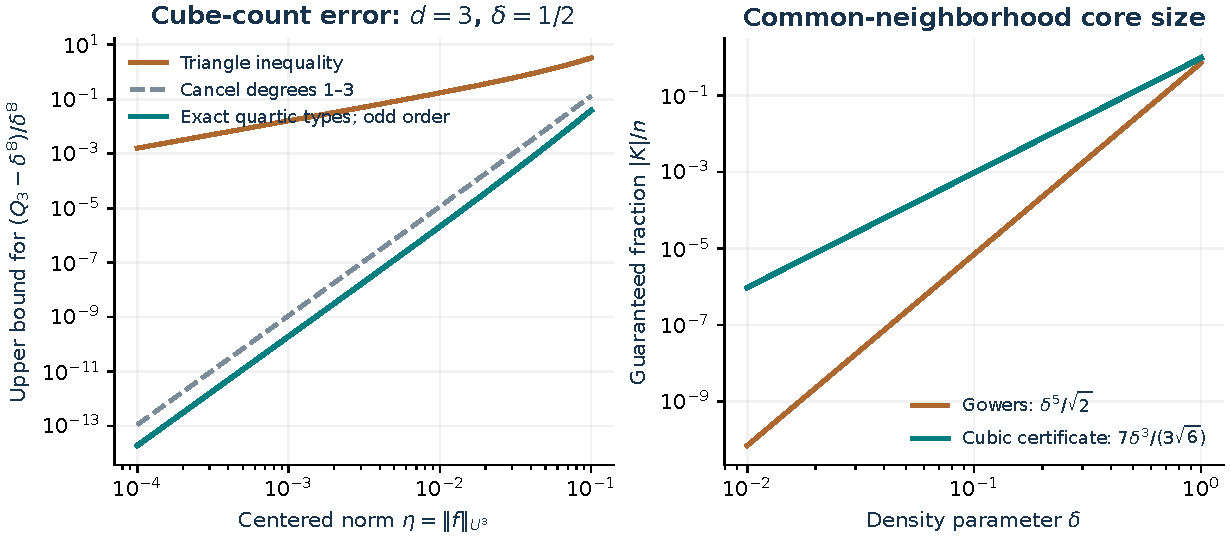
\includegraphics[width=\textwidth]{figures/03-local-estimates-local_bound_comparisons.pdf}
\caption{Evaluations of proved local bounds. Left: relative cube-count
error bounds for $d=3$, $\delta=1/2$, comparing the triangle inequality,
the cancellation of degrees one through three, and the exact quartic
types on an odd-order group. Right: guaranteed core fractions at the
same threshold $\delta^2m/2$ and the same $90\%$ good-pair requirement.
These are upper or lower bounds as labelled, not measurements of
extremal examples or claims that each curve is attainable.}
\label{gsr:fz:03:fig:comparisons}
\end{figure}
\FloatBarrier

\subsection{An explicit abstract recurrence}

The following elementary calculation explains which parameters must be
tracked before any global conclusion can be stated. It is a conditional
recurrence theorem, not a substitute for the analytic density increment
theorem needed to supply its hypotheses.

\begin{proposition}[Density and length bookkeeping]
\label{gsr:fz:03:impact:recurrence}
Let $c>0$, $p>1$, $C>0$, $q\ge0$, and $0<\beta<1$. Suppose positive
numbers $\delta_i\le1$, $N_i>0$ satisfy, for $0\le i<R$,
\[
 \delta_{i+1}\ge\delta_i+c\delta_i^p,
 \qquad N_{i+1}\ge C\delta_i^q N_i^\beta.
\]
Then
\begin{equation}
 R\le\frac{(1+c)^p}{c(p-1)}
                 \bigl(\delta_0^{1-p}-1\bigr).
 \label{gsr:fz:03:impact:steps}
\end{equation}
Writing $B=\max\{0,-\log(C\delta_0^q)\}$, one also has
\begin{equation}
 \log N_r\ge\beta^r\log N_0
             -B\frac{1-\beta^r}{1-\beta}
 \qquad(0\le r\le R).
 \label{gsr:fz:03:impact:length}
\end{equation}
Consequently, for an integer $T\ge R$ and $H\ge1$, the condition
\begin{equation}
 \log N_0\ge\beta^{-T}
                  \left(\log H+\frac{B}{1-\beta}\right)
 \label{gsr:fz:03:impact:budget}
\end{equation}
ensures $N_r\ge H$ at every $r\le R$.
\end{proposition}

\begin{proof}
The potential $u^{1-p}$ decreases at a controlled rate. Since
$\delta_i\le1$,
\begin{align*}
 \delta_i^{1-p}-\delta_{i+1}^{1-p}
 &\ge (p-1)\int_{\delta_i}^{\delta_i+c\delta_i^p}t^{-p}\,dt\\
 &\ge\frac{(p-1)c\delta_i^p}{(\delta_i+c\delta_i^p)^p}
 \ge\frac{(p-1)c}{(1+c)^p}.
\end{align*}
Summing and using $\delta_R^{1-p}\ge1$ gives~\eqref{gsr:fz:03:impact:steps}.
The densities are increasing, so
$\log N_{i+1}\ge\beta\log N_i-B$.
Iterating this affine inequality gives~\eqref{gsr:fz:03:impact:length}.
Under~\eqref{gsr:fz:03:impact:budget}, $\beta^r\log N_0$ is at least
$\log H+B/(1-\beta)$ for $r\le T$, which proves the last assertion.
\end{proof}

For fixed constants, the familiar double-exponential length budget is
visible in~\eqref{gsr:fz:03:impact:budget}: the number of iterations occurs in the
exponent of $\beta^{-T}$, which already bounds a logarithm of the
starting size. Improving $C$ or $q$ changes the additive length cost $B$.
Improving the density growth exponent $p$ can change the scale of the
number of iterations. These are different effects. To extract a better
global Szemer\'edi bound from this report one would have to identify,
and prove throughout the later sections, the corresponding updated
values or functions of all these parameters. We have not carried out
that full replacement of the higher-order inverse and localization
arguments.
\begin{writenote}[6 October 2026; sources 06--10]
\emph{Two further iteration statements.} Source~10's Proposition~\ref{gsr:fz:10:prop:iteration} bounds the number of steps of the same recurrence by $(\delta_0^{1-p}-1)/(1-(1+c)^{1-p})$, and source~06's Lemma~\ref{gsr:fz:06:iter:potential} with $G=1$ by $1+(\delta_0^{1-p}-1)/(c(p-1))+p\log(1/\delta_0)$ (its \eqref{gsr:fz:06:iter:power-count}). \emph{Comparison (second write).} With $q=p-1$, $1-(1+c)^{-q}=q\int_0^c(1+u)^{-q-1}du$ lies between $qc(1+c)^{-q-1}$ and $qc$, so the coefficients of $\delta_0^{1-p}$ satisfy $1/(cq)\le1/(1-(1+c)^{-q})\le(1+c)^p/(cq)$: source~06's leading coefficient is the smallest and source~10's lies between it and the one in \eqref{gsr:fz:03:impact:steps}; source~06's bound has the additional term $1+p\log(1/\delta_0)$ and counts the densities $\delta_0,\ldots,\delta_{t-1}$, whereas the bound here counts steps. For $p=2$, $c=1/320$ the coefficients are $320$, $321$ and $321^2/320\approx322.003$. Source~06 also proves that the leading term of its double-logarithmic length budget is optimal for its abstract local rule (its Section~\ref{gsr:fz:06:sec:d6}), and source~10's Proposition~\ref{gsr:fz:10:prop:length-iteration} is the length recursion \eqref{gsr:fz:03:impact:length} with variable parameters.
\end{writenote}

The same distinction applies to the exact quartic identity. It is
stronger information about cubes with a prescribed balanced Gowers norm.
It does not imply that every set lacking arithmetic progressions has a
large ordinary Fourier coefficient. Gowers's motivating examples address
precisely why higher-order structure is needed. The role of the improved
count is to make the uniformity branch and its constants more precise.

\section[{The Lean development and a concrete formalization route\srctag{03}}]{The Lean development and a concrete formalization route}\label{gsr:fz:03:sec:d10}
\srcnote{03}{Section 10}
\label{gsr:fz:03:sec:formal}

\subsection{Pinned source and status of the inspection}

All repository comparisons refer to revision
\begin{center}\small\revision\end{center}
of \repo, inspected on 6 October 2026. The requested paper is at
\path{Combinatorics/Ramsey/Papers/sz-thm-gowers-proof}; the Lean files
are at \path{Combinatorics/Ramsey/Lean/GowersSzemeredi}.
The adjacent source inventory, \path{gowers-proof-status.json}, reports
88 numbered statements with exact companion declarations and 32 open
statements at that revision \cite{repo03status}.
\begin{writenote}[6 October 2026]
\emph{Stale since the pin.} At HEAD (\texttt{25df8755d}, 6~October 2026) the inventory records 98 exact companions and 22 open statements. The ten statements closed since \texttt{3a25020a6} are \file{corollary_5_6}, \file{corollary_5_7}, \file{lemma_5_9}, \file{lemma_5_10}, \file{corollary_5_11}, \file{lemma_5_14}, \file{lemma_16_1}, \file{lemma_16_3}, \file{lemma_16_5} and \file{lemma_16_6} (compared at the write). \file{theorem_1_3}, \file{theorem_18_1} and \file{theorem_18_2} are still open, so the conclusion of the next paragraph stands. Crosswalk: Section~\ref{gsr:fz:sec:crosswalk}.
\end{writenote}

Those counts are a source inventory, not a certification of the whole
development. The facade exposes numbered results as propositions, usually
with companion theorems whose names end in \texttt{\_holds}. Defining a
proposition neither proves it nor adds it as an axiom. The inventory
explicitly separates exact companions from conditional, restricted, or
otherwise related results. In particular, the quantitative headline
\texttt{theorem\_1\_3} and final statements
\texttt{theorem\_18\_1} and \texttt{theorem\_18\_2} are marked open
there. This inspection therefore does not support describing the
repository as a completed formal proof of the full quantitative theorem.

The files directly relevant to our comparisons contain substantive
companion proofs. We inspected their definitions and proof scripts; we did
not compile the Lean project. The new mathematical statements in this
report have written proofs and independent mathematical reviews, together
with the finite checks described in the appendix. No new machine-checked
Lean proof is claimed or supplied.
\begin{writenote}[6 October 2026]
The ``independent mathematical reviews'' mentioned here and in Section~\ref{gsr:fz:03:sec:dA} are not part of the delivery and are not recorded anywhere in the repository; this report relies on the printed proofs, the intake's checks and the write's notes, not on them.
\end{writenote}

\subsection{Normalization map}

The following conversions prevent a common source of false improvements.
Let $N=|G|$, and take $d\ge1$.

\begin{center}
\small
\begin{tabularx}{\textwidth}{@{}p{0.24\textwidth}X X@{}}
\toprule
Quantity & This report & Inspected repository convention\\
\midrule
Fourier transform & $\E_x f(x)\overline{\chi(x)}$ & Unnormalized sum,
equal to $N$ times this transform\\
Gowers norm & $\|f\|_{U^d}$ &
$\texttt{gowersNorm}\ d\ f=N^{(d+1)/2^d}\|f\|_{U^d}$\\
Uniformity parameter & $\|f_A\|_{U^d}^{2^d}\le\alpha$ &
$\texttt{UniformSetOfDegree}\ A\ \alpha\ (d-1)$\\
Cube count & $Q_d(\1_A)$ &
$\texttt{cubeCount}=N^{d+1}Q_d(\1_A)$\\
Cube arguments & $x+\sum_i v_i h_i$ & A minus convention in
\texttt{cubeArgument}; negating all $h_i$ gives the same average\\
\bottomrule
\end{tabularx}
\end{center}

Both cube conventions count all parameter tuples, including degenerate
cubes. This is why the rounding lemma can bound the exceptional tuples
by a collision probability instead of changing the definition of the
norm. Changing to unlabelled, injective, or symmetry-quotiented cubes
would require an additional counting theorem.

\subsection{Useful existing declarations}

The source provides the following starting points in namespace
\path{LeanProofs.GowersSzemeredi}. These are concrete interfaces to
reuse or generalize, rather than assertions that the proposed additions
have already been formalized.

\begin{description}[style=nextline,leftmargin=1em]
\item[Partition discrepancy and Fourier increment.]
\path{Proofs02DensityIncrement.lean} proves
\path{corollary_2_5_holds}. Its private
\path{cor25_large_scale} already obtains the stronger $\rho/4$
increment and $\sqrt{\rho N/(128\pi)}$ length before weakening its
conclusion. General finite weighted sums, followed by
Theorem~\ref{gsr:dt:03:selection:sharp}, would expose the asymmetric information
without repeating the Fourier argument.

\item[Multilinear norms and cube expansion.]
\path{Proofs03GowersCS.lean} contains the public homogeneous theorem
\path{gowers_cauchy_schwarz}, which already allows functions beyond the
unit disc. \path{Proofs03Minkowski.lean} contains the triangle inequality
and private distributive expansion helpers.
\path{Proofs03CubeUpper.lean} proves \path{lemma_3_10_holds} from that
triangle inequality. Exporting a general expansion indexed by vertex
subsets is a natural first step toward the exact quartic theorem.

\item[Selection from many cells.]
\path{Proofs05_10.lean} contains \path{lemma_5_15_holds}. Its assumptions
and conclusion match the symmetric discrepancy extraction discussed in
Section~\ref{gsr:dt:03:sec:selection}. The general theorem should be stated with
real nonnegative cell weights and asymmetric cell-sum bounds, then
specialized to cardinalities.

\item[Dependent random choice.]
\path{Proofs07DRC.lean} proves \path{lemma_7_4_holds} using ordered
samples with replacement, indexed by \path{Fin 5}. Its internal score
bound already has constant $11/16$ multiplying $\delta^{10}n^2$.
The main new ingredient for the cubic theorem is a pointwise polynomial
minorant, followed by the exact three-sample counting identity. Merely
exposing the internal five-sample constant would give a smaller change.
\end{description}

\subsection{Recommended order of implementation}

First formalize the finite weighted selection theorem over an arbitrary
finite index type. Prove positivity of its denominators once, and keep
the pointwise inequalities separate from the division steps. This
produces immediately reusable specializations to Lemma~5.15 and balanced
indicators.

Second formalize the cubic certificate. Its good-region proof is a
polynomial identity followed by nonnegativity; its bad-region proof may
use concavity or a direct monotonicity argument. Keep the sampling
identity generic in the number of witnesses. Specialization to three
witnesses then replaces only the numerical part of the current DRC
proof.

Third export the general cube expansion and prove the single-coordinate
cancellation lemma. Nonempty supports of at most three selected vertices, or four vertices
with nonzero XOR, leave one variable occurring in exactly one centered
factor after a coordinate reflection. The corresponding reindexing is
a bijection and uses no division by two. The first quartic upper bound
then follows directly from Gowers--Cauchy--Schwarz, before any Fourier
classification is needed.

Fourth formalize the two nonzero four-vertex types. One may begin over
$\Z/N\Z$ to match existing files, then generalize to finite abelian
groups. The extra quotient energy requires explicit handling of order-two
characters; assuming an invertible doubling map is appropriate only for
the odd-order specialization. The combinatorial formulas for $R_d,T_d$
are separate finite enumeration theorems.

Finally integrate the progression-count telescope, the proper progression
partition, and the four-edge compression statement. Each has a clear
finite interface. The generalized von Neumann theorem should state
invertibility of slope differences explicitly; the progression partition
should carry its lower and upper integer lengths in its output. This
order establishes useful lemmas early while avoiding dependence on the
unfinished quantitative headline.

\section[{Further research questions and topics\srctag{03}}]{Further research questions and topics}\label{gsr:fz:03:sec:d11}
\srcnote{03}{Section 11}
\label{gsr:fz:03:sec:research}

The following questions are proposed continuations of the proved results.
Some are deliberately scoped finite problems, while others concern the
larger proof architecture. A question proposed here is not being presented
as a previously published open problem unless a source is identified.

\begin{problem}[The odd-order leading constant]
\label{gsr:fz:03:question:oddconstant}
For fixed $d\ge3$, determine
\[
 c_d^{\rm odd}=\sup_{\substack{G\text{ finite abelian, }|G|\text{ odd}\\
                     0\ne f:G\to\R,\ \E f=0}}
       \frac{\|f\|_{U^2}^4}{\|f\|_{U^d}^4}.
\]
The exact quartic theorem reduces the best leading coefficient on
odd-order groups to $R_dc_d^{\rm odd}$. Is the supremum attained or
approached by a real part of a character, by several Fourier modes, or
by a different construction?
\end{problem}

The universal bound $c_d^{\rm odd}\le1$ follows from monotonicity.
Our cosine example gives a positive explicit lower bound. The order-two
character that attains the unrestricted coefficient is unavailable here,
so the sharp universal result does not settle this restricted problem.
A practical first project is a systematic search over small odd cyclic
groups, followed by an inequality explaining any apparent extremizer.
Numerical optimization would be evidence, not a proof of the supremum.
\begin{writenote}[6 October 2026]
\emph{Settled for $d=3$ (cross-source finding).} Source~04's Theorem~\ref{gsr:cc:04:cub:norm-gap} gives $c_3^{\mathrm{odd}}=2^{-1/2}$, attained exactly by the real parts $2\operatorname{Re}(c\xi)$ of nontrivial characters (the question's first alternative); proof in the note after that theorem. The best odd-order leading coefficient for $d=3$ is $R_3c_3^{\mathrm{odd}}=6\sqrt2$, as source~04 proves directly. For $d\ge4$ the question is open; it coincides with source~04's Question~3 (Section~\ref{gsr:fz:sec:further}, item~\ref{gsr:fz:q:III:normgap}).
\end{writenote}

\begin{problem}[Classify the fifth and sixth centered coefficients]
For each $r=5,6$, classify the supports $S\subseteq\{0,1\}^d$ of size
$r$ for which the character system~\eqref{gsr:cc:03:cube:fullfourier} can have
solutions with no trivial character. Derive multiplicities as functions
of $d$ and identify the necessary quotient correlations and Fourier phase
invariants.
\end{problem}

The coordinate-reflection test removes every support with a coordinate
occupied by exactly one selected vertex or by all but one. For surviving
supports, Smith invariant factors identify possible small-torsion
obstructions. A successful classification should distinguish actual
vanishing of a centered correlation from mere rational independence of
its defining forms. The fifth-order examples discussed at the end of
Section~\ref{gsr:cc:03:cube:section} give concrete starting cases.
\begin{writenote}[6 October 2026; sources 06--10]
\emph{Fifth order answered, sixth order open.} For $r=5$ the question is answered by source~09's Theorems~\ref{gsr:cc:09:thm:five-class} and~\ref{gsr:cc:09:thm:main} with Proposition~\ref{gsr:cc:09:prop:five-count}: two support types, multiplicities $Q_d$ and $S_d$, and the correlations $\Mfive$ (order-two coupling $\chi,\chi^2$) and $\Tthree$ (order-three characters). For $r=6$ it remains open; source~09 shows that an isolated order-five term occurs there (Theorem~\ref{gsr:cc:09:thm:5torsion}) and asks the same question (Section~\ref{gsr:fz:sec:further}, item~\ref{gsr:fz:q:III:fifth}).
\end{writenote}

\begin{problem}[The sharp fixed-threshold DRC profile]
Let $F(\delta)$ be the largest guaranteed fraction $|K|/n$ under the
exact hypotheses and success criterion of Lemma~7.4. Determine the
correct order of $F(\delta)$ as $\delta\downarrow0$. Can the exponent
$3$ in Theorem~\ref{gsr:en:03:drc:cubic-selection} be improved using constraints
specific to intersection matrices?
\end{problem}

The scalar optimization proves only that a particular two-witness
first-moment certificate cannot give a positive uniform estimate at the
original parameters. Actual overlap matrices are symmetric positive
semidefinite Gram matrices of indicators and obey further incidence
constraints. It is a real additional problem to determine whether those
constraints rule out the scalar bad distributions. Conversely, a lower
bound on the necessary exponent requires realizable families of sets,
not just a distribution of formal overlap values.

\begin{problem}[Optimize the entire elementary extraction]
Optimize the three parameters $\gamma,\varepsilon,\beta$ in
Proposition~\ref{gsr:en:03:drc:graph-compression}, and compare alternative walk
lengths and popularity thresholds. Which size--difference-set tradeoffs
can be achieved while retaining only elementary finite inequalities?
\end{problem}

The meaningful objective is the pair of conclusions, including the
normalization of the difference-set bound by $|A|$ or by $|A'|$.
Optimizing one displayed exponent while allowing the selected set to
shrink excessively can conceal a loss. Comparison with
\cite{reiherschoen} should remain explicit; the purpose of this project
would be a simple formalizable proof or a better constrained tradeoff,
not to mistake an elementary refinement for an improvement of the
strongest known theorem.

\begin{problem}[Allocate phase oscillation by local mass]
Suppose a phase partition can be refined at a cost depending on the
desired oscillation in each cell. Can one minimize the total refinement
cost subject to
\[
 \sum_j\int_{P_j}|f|\,|\psi_j-z_j|\,d\mu\le\lambda\rho
\]
by using local information on $|f|$, rather than a single global
oscillation tolerance?
\end{problem}

Lemma~\ref{gsr:dt:03:selection:phase} already provides the exact analytic constraint.
The unresolved work is geometric: prove a refinement theorem with a
cost function sharp enough for this optimization to matter. One can
start with linear phases and known cell masses, then study polynomial
phases. The global density factor in Theorem~\ref{gsr:dt:03:phase:increment} is
the simplest instance of retaining this information.

\begin{problem}[Local counting that rectifies automatically]
Develop a version of Theorem~\ref{gsr:cc:03:ap:telescoping} for interval-supported
functions or localized norms in which the conclusion directly counts
ordinary integer progressions and includes all boundary errors.
\end{problem}

The elementary second-difference test gives a clean sufficient condition
for rectification, but the global modular norm does not enforce that
condition. The target is an explicit statement whose hypotheses reflect
both uniformity and support. Any proposed bound should be tested on
sets concentrated near the ends of the interval and on small composite
moduli before it is fed into the density increment iteration.

\begin{problem}[Propagate improvements through a verified dependency graph]
Replace the improved local lemmas in the later sections of the proof,
record every dependence of density, progression length, dimension, and
correlation on earlier parameters, and obtain a complete explicit
iteration theorem.
\end{problem}

Proposition~\ref{gsr:fz:03:impact:recurrence} specifies the final bookkeeping for
one common type of increment. The hard work is to prove the hypotheses
with the newly propagated functions. An initial useful deliverable would
be a symbolic parameter dependency graph accompanied by Lean theorems
for each monotone substitution. This would reveal which improvements
survive and which are absorbed by later losses, even if the final
asymptotic class stays unchanged.

\begin{problem}[Quantitative rounding and efficient derandomization]
Optimize the group-size requirement for the sharpness constructions at
a given error tolerance, including the exact-density version of
Corollary~\ref{gsr:cc:03:cube:exactdensity}. Can one derandomize the rounding with
an efficient finite algorithm?
\end{problem}

The existence problem at a compatible prescribed rational density is
already solved by the slow perturbation and small alteration in
Corollary~\ref{gsr:cc:03:cube:exactdensity}. Its size requirement is deliberately
generous. Sampling directly with a fixed total, a sharper norm estimate
for the alteration, or a deterministic conditional-expectation argument
might improve it. Independence no longer applies unchanged after
conditioning on cardinality, so that approach needs its own estimate.

\begin{problem}[A reusable formal library of centered configuration counts]
Build a finite-abelian-group library whose basic objects are systems of
integer linear forms, centered multilinear averages, character constraint
sets, and explicit reindexing bijections. Recover the cube and progression
results as specializations.
\end{problem}

The key interface should retain integer torsion data. A proof over
$\Q$ alone does not control evaluation on all finite groups. At the same
time, the library should make cancellation by a single free variable
easy, so simple cases do not require a full Smith normal form calculation.
This is an achievable software and formalization project with reusable
mathematical outputs, independent of completing the entire Gowers proof.

\section[{Reproducibility and verification\srctag{03}}]{Reproducibility and verification}\label{gsr:fz:03:sec:dA}
\srcnote{03}{Appendix A}
\label{gsr:fz:03:appendix:checks}

The accompanying archive contains the complete LaTeX source and compiled
PDF, the figure in vector PDF form, scripts for the figure and finite
checks, and the recorded check output. No original third-party paper is
repackaged. The repository revision and source paths are recorded so that
the comparisons can be repeated against the same input.

\subsection{What the scripts check}

\path{verify_cubes.py} uses only the Python standard library and exact
rational arithmetic. It enumerates every four-vertex support of the
Boolean cube for dimensions two through five. In dimension five this
means all $\binom{32}{4}=35960$ supports. It compares a classification
from minors with a separate classification from XOR and coordinate
patterns. The counts are exactly those in Lemma~\ref{gsr:cc:03:cube:counts}.
It also computes the coefficients of the full cube polynomial directly,
without using the proposed quartic formula, on cyclic groups of orders
two through six in dimensions two and three. The low-degree
cancellations, torsion correction, and parity polynomial all pass.

\path{verify_estimates.py} checks the sharp selection extremizers with
exact rational weights, evaluates the cubic certificate including its
boundary and tangent cases, constructs proper phase partitions at
several finite scales, and enumerates all subsets of $\Z/5\Z$ and
$\Z/7\Z$ for the progression bounds at lengths three and four.
The norm powers in the latter check are rational; taking roots and
comparing the bounds uses floating-point arithmetic with an explicit
tolerance. The phase oscillation checks are also numerical. These are
clearly distinguished from the exact cube and scalar checks.

Independent written reviews checked the asymmetric selection extremizers,
finite progression geometry, Cauchy--Schwarz induction, quartic support
classification and Bernoulli rounding, cubic minorant, and four-label
counting injection. These reviews and finite computations are useful
error checks; the proofs in the article, rather than the tested finite
range, justify the theorems for arbitrary parameters.

\subsection{Building the document}

\begin{samepage}
From the extracted directory, run
\begin{verbatim}
python3 verify_cubes.py
python3 verify_estimates.py
pdflatex -interaction=nonstopmode -halt-on-error gowers_local_refinements.tex
pdflatex -interaction=nonstopmode -halt-on-error gowers_local_refinements.tex
\end{verbatim}
\end{samepage}
The figure is already included, so compiling the document does not
require Python or a plotting library. To regenerate the figure, run
\path{make_figure.py} in an environment with NumPy and Matplotlib.
The LaTeX source uses standard packages including AMS mathematics,
Palatino fonts, \path{microtype}, \path{booktabs}, and \path{hyperref}.

\section[{Quantitative comparisons and what they enable\srctag{04}}]{Quantitative comparisons and what they enable}\label{gsr:fz:04:sec:d9}
\srcnote{04}{Section 9}
\label{gsr:fz:04:sec:comparisons}

The preceding results address different sources of loss.  Their benefits
should therefore be read at the interface where each estimate is used.
The following table records those interfaces without combining unrelated
parameters into a single claimed global improvement.

\begin{table}[htbp]
\centering
\small
\renewcommand{\arraystretch}{1.25}
\begin{tabularx}{\textwidth}{@{}>{\raggedright\arraybackslash}p{0.20\textwidth}>{\raggedright\arraybackslash}X>{\raggedright\arraybackslash}X@{}}
\toprule
Interface & Coarse source estimate & Strengthened estimate here\\
\midrule
Graph moment, input \(\gamma|B|^3\)
& \(\gamma^7\beta^{21}p^{15}\)
& \(\gamma^7\beta^{15}p^{15}\); arbitrary moment order and equality cases\\
Almost-homomorphism restriction, order eight
& \((\gamma^7\beta^6\eta/4)^{2^{19}}|B|^{15}\)
& \(2^{-95}\gamma^{112}\eta^{15}|B|^{15}\), under the explicit size hypothesis in Corollary~\ref{gsr:en:04:rest:eight}\\
Three-cube upper bound, \(u=\|f\|_{U^3}\)
& \((\delta+u)^8\)
& Excess begins with \(6\sqrt2\,\delta^4u^4\), with explicit higher terms\\
\(k\)-term progression counting
& Error bounded by \(2^k u\)
& Error bounded by \(u\sum_{j=0}^{k-3}\delta^j\)\\
Section 17 local coefficient
& \(2^{-2(k+1)^3}\)
& \(2^{-k^2-k\log_2 k-O(k)}\), with an explicit constant\\
\bottomrule
\end{tabularx}
\caption{Comparisons with the specified local estimates in
\cite{gowers,repo04}.  The variables and hypotheses are those of the
corresponding sections.  The improved restriction theorem includes a
large-field condition, and the phase theorem includes a characteristic
condition.}
\label{gsr:fz:04:tab:comparisons}
\end{table}

The field-size requirement in the restriction theorem has a particularly
simple interpretation:
\[
 |B|\geq \Lambda_d(\alpha\eta)^{-2d}.
\]
The ambient density does not otherwise enter this sufficient condition.
Two elementary decisions are responsible.  A rank-two exceptional relation
leaves at most \(|B|^{2d-2}\) tuples, because its free coordinates can be
chosen from \(B\).  These contributions are then summed with their
nonnegative Fourier weights, whose total is at most one.  Thus the number
of possible coefficient vectors does not enter the error bound.
Repeated entries are handled separately.  These refinements are useful
even before any attempt to optimize the kernel.

For an illustrative comparison, take \(\gamma=\eta=\beta=1/2\).
The retained fraction of \(|B|^{15}\) in the source display is
\(2^{-8\,388\,608}\), whereas the convenient bound here is \(2^{-222}\).
The corresponding sufficient field-size condition here is
\(p\geq2^{231}\).  These are deliberately transparent evaluations of the
proved formulas, not practical finite-size estimates.  They show the
change in parameter dependence and also the cost of the conservative
exceptional-tuple estimate.

\begin{figure}[htbp]
\centering
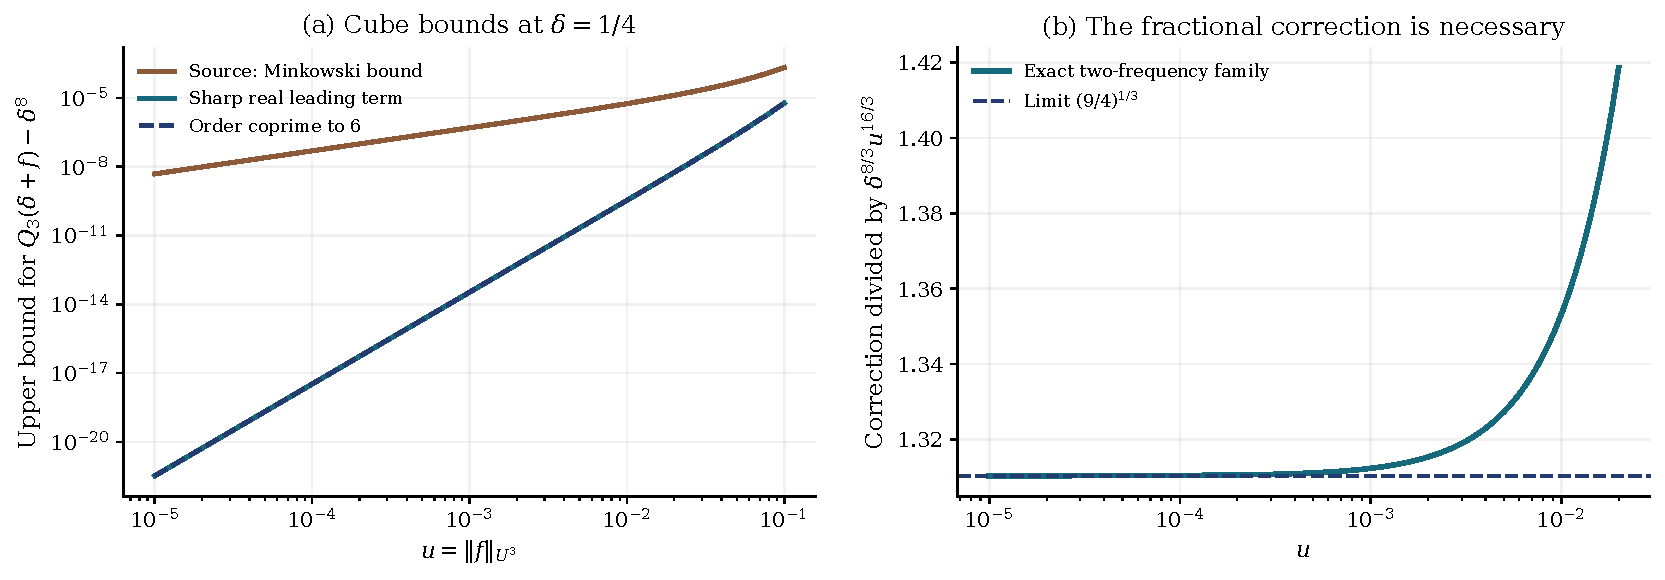
\includegraphics[width=\textwidth]{figures/04-restriction-cubes-cube_refinements.pdf}
\caption{Proved bounds and an exact extremizing model at \(\delta=1/4\).
Left: the excess above \(\delta^8\) in the source triangle-inequality
bound and the two refined bounds of
Theorems~\ref{gsr:cc:04:cub:main} and~\ref{gsr:cc:04:cub:fractional}.  The refined curves nearly
coincide at small \(u\) because they have the same sharp leading term.
Right: after subtracting that leading term, the explicit two-frequency
family of Proposition~\ref{gsr:cc:04:cub:two-frequency}, divided by
\(\delta^{8/3}u^{16/3}\), tends to \((9/4)^{1/3}\).
The figure evaluates formulas; it is not a statistical fit.}
\label{gsr:fz:04:fig:cubes}
\end{figure}

The cube results answer two precise local extremal questions.
The best universal leading coefficient in the real centered, odd-order
setting is \(6\sqrt2\).  In the setting without \(2\)- or \(3\)-torsion,
the first possible correction after that leading term has optimal
exponent \(16/3\).  What remains undetermined is the exact coefficient
of this correction and the existence of a universal asymptotic expansion
for the extremal envelope.  These are local conclusions with explicit
models, independent of any claim about the best quantitative bound for
arithmetic-progression-free sets.

\section[{Further research questions and a proposed program\srctag{04}}]{Further research questions and a proposed program}\label{gsr:fz:04:sec:d10}
\srcnote{04}{Section 10}
\label{gsr:fz:04:sec:research}

The questions below are proposed research targets arising from the
calculations.  The list distinguishes exact optimization problems from
larger integration projects.  It is not a claim that each formulation is
already recognized as an open problem in the literature; a more extensive
priority review should accompany work toward publication.

\subsection{Extremal cube counts}

\begin{enumerate}[label=\textbf{Q\arabic*.},leftmargin=2.6em]
\item \textbf{Does the secondary extremal coefficient exist, and what is it?}
Fix \(0<\delta<1\), and let \(M_\delta(u)\) be the supremum of
\(Q_3(W)\) over prime cyclic groups of order greater than \(16\) and weights
\(0\leq W\leq1\) satisfying
\(\E W=\delta\) and \(\|W-\delta\|_{U^3}=u\).
Theorems~\ref{gsr:cc:04:cub:fractional} and
Proposition~\ref{gsr:cc:04:cub:two-frequency} imply
\[
 (9/4)^{1/3}
 \leq
 \liminf_{u\downarrow0}
 \frac{M_\delta(u)-\delta^8-6\sqrt2\,\delta^4u^4}
      {\delta^{8/3}u^{16/3}}
 \leq
 \limsup_{u\downarrow0}
 \frac{M_\delta(u)-\delta^8-6\sqrt2\,\delta^4u^4}
      {\delta^{8/3}u^{16/3}}
 \leq6.
 \tag{Q1}
\]
Determine whether the limit exists.  Is the two-frequency value
\((9/4)^{1/3}\) optimal?  A useful first step is a sharper estimate of the
quintic correlation in terms of the exact loss in the norm-gap inequality,
instead of the separate bounds used above.

\item \textbf{What is the correct stability statement for cube extremizers?}
Corollary~\ref{gsr:cc:04:cub:gap-stability} controls the fourth-power Fourier mass
outside one conjugate pair, equivalently a \(U^2\) remainder.  This does
not alone control an \(L^2\) remainder: many small Fourier coefficients
can have little fourth-power mass but substantial second-power mass.
Determine the strongest stability conclusion for bounded weights that
nearly attain the leading cube bound, and identify any additional
hypothesis needed for a stronger metric.  For near optimal secondary
behavior, test whether concentration on frequencies
\(\{\pm\xi,\pm2\xi\}\) follows.

\item \textbf{What replaces the sharp norm gap in higher dimensions?}
For \(d\geq4\), determine the best constant in the comparison of
\(\|f\|_{U^d}^{2^d}\) and \(\|f\|_{U^2}^{2^d}\) for real centered
functions, specifying the allowed group orders.  Combine it with the
exact coefficient \(P_d\) of Proposition~\ref{gsr:cc:04:cub:quartic}.
The Boolean support matroid gives a finite organizing device for the
next correlations, but their values and sharp norm bounds require
additional harmonic analysis.  Separate large-characteristic behavior
from the extra identities produced by small torsion.
\begin{writenote}[6 October 2026]
For $d=3$ the comparison is Theorem~\ref{gsr:cc:04:cub:norm-gap}; for $d\ge4$ this is source~03's Research question~\ref{gsr:fz:03:question:oddconstant} (which asks for the constant over odd-order groups). Merged in Section~\ref{gsr:fz:sec:further}, item~\ref{gsr:fz:q:III:normgap}.
\end{writenote}
\end{enumerate}

\subsection{Restriction and moment estimates}

\begin{enumerate}[label=\textbf{Q\arabic*.},leftmargin=2.6em,resume]
\item \textbf{Can the size threshold be substantially lowered?}
Theorem~\ref{gsr:en:04:rest:main} requires
\(|B|\geq\Lambda_d(\alpha\eta)^{-2d}\).
The proof already controls exceptional relations in expectation using
their Fourier weights.  Can their contribution be made to reflect the
additive structure of \(B\), rather than the uniform rank-two bound?
Can a kernel with a more favorable coefficient distribution reduce the
required size without weakening the retained tuple count?  Any proposed
improvement must handle repeated entries as well as extra relations among
distinct entries.

\item \textbf{What is the true optimal retention law?}
The bound
\(\kappa_d\alpha^{2d}\eta^{2d-1}|B|^{2d-1}\) has the natural parameter
powers for the single-kernel expectation budget in
Proposition~\ref{gsr:en:04:rest:method-bound}.  That proposition does not establish
optimality among all selection procedures.  Construct upper-bound
examples, or find a different selection method with better powers.
Also ask for useful simultaneous guarantees on \(|B'|\), its ordinary
additive energies, and the density of respected relations.

\item \textbf{How far does restriction extend beyond prime cyclic groups?}
The interpolation theorem already applies to arbitrary finite abelian
groups.  The restriction theorem uses a field to turn two independent
linear equations into a uniform bound on the number of solutions.
Develop versions for \(\mathbb Z/N\mathbb Z\), finite-field vector
spaces, and maps into other groups.  The appropriate hypotheses should
quantify kernels of the relevant coefficient maps, rather than silently
treat nonzero determinants as invertible.  A weighted formulation would
also allow nonuniform input measures.

\item \textbf{Can the cross-section profile be propagated through the proof?}
For arrangements the gain is governed by
\(\sigma=\E_r\beta_r^3\), not just by the global density.
Track this profile through subsequent restrictions and changes of
variables.  Determine which operations preserve useful control of
\(\sigma\), and whether a collection of higher cross-section moments
gives a stronger interface than a single density parameter.  Equality
models in Section~\ref{gsr:en:04:mom:arrangement-section} provide tests against
overly optimistic exponents.
\end{enumerate}

\subsection{Patterns, counting, and integration}

\begin{enumerate}[label=\textbf{Q\arabic*.},leftmargin=2.6em,resume]
\item \textbf{Determine the asymptotics of the fractional pattern counts.}
The proved estimates imply
\[
 \tfrac12
 \leq\liminf_{k\to\infty}\frac{\log_2 F_k}{k^2}
 \leq\limsup_{k\to\infty}\frac{\log_2 F_k}{k^2}
 \leq1,
 \tag{Q2}
\]
and the same bounds for \(A_k\).
Determine the leading constant, or improve the gap in these bounds.
Relate the particular affine arrangements here to established results
on threshold patterns and subset-sum arrangements before assigning
novelty.  Exact certified counts for \(k=4\) are a concrete computational
next step; exploiting symmetries is likely to matter more than merely
using a faster numerical solver.
\begin{writenote}[6 October 2026]
\emph{Answered by source~01} (cross-source finding of the intake, checked at the write). The $F_k$ here is source~01's $C_k$ and the $A_k$ here is source~01's $A_k$: the definitions are identical. Source~01's Theorem~\ref{gsr:fp:01:thm:carryasymptotic} gives $k^2-k\log_2k-O(k)\le\log_2C_k\le k^2+(\log_2e-1)k$. Its Theorem~\ref{gsr:fp:01:thm:affine} gives $C_k\le A_k$ and $\log_2A_k\le k^2+O(k)$. Hence both limits in (Q2) exist and equal $1$. The lower half uses one external input, the classical threshold-function count (Zuev; Kahn--Koml\'os--Szemer\'edi, as recorded by Baldi--Vershynin \cite{bv}), which source~01 cites and does not reprove. Source~01's Proposition~\ref{gsr:fp:01:prop:counts} certifies $F_4=C_4=154$, the ``concrete computational next step'' asked for. $A_4$ is not certified (an uncertified recount gives $770$), and the secondary term is source~01's first question; both remain open (Section~\ref{gsr:fz:sec:further}, items~\ref{gsr:fz:q:IV:counts} and~\ref{gsr:fz:q:IV:second}).
\end{writenote}
\begin{writenote}[6 October 2026; sources 06--10]
Source~06 answers the same question independently: its Theorem~\ref{gsr:fp:06:car:entropy} gives $\log_2C_k=(1+o(1))k^2$ and $\log_2D_k=(1+o(1))k^2$ (the same external threshold count), uniformly modulo every $M\ge2$, and its Section~\ref{gsr:fp:06:sec:d7} certifies $C_4=154$ a second time.
\end{writenote}

\item \textbf{Which global and local profiles are actually realizable?}
The phase-extraction proof uses the uniform bound \(2^k\) for the
profiles at a fixed slope and an arrangement bound for all slopes.
The slopes there come from a short discrete interval.  Determine the
joint distribution of profiles in that arithmetic setting, including
small moduli \(M\), and test whether an average multiplicity can replace
the worst-case local multiplicity.  The exact modular formula of
Theorem~\ref{gsr:fp:04:pat:scaling} isolates one source of collisions.

\item \textbf{Can progression counting use more of the mixed information?}
The dynamic program in Section~\ref{gsr:cc:04:sec:progressions} finds the best
bound within a specified telescoping family.  It is not an optimality
theorem for all counting arguments.  Investigate whether mixed
uniformity norms, additional cancellations, or information about
particular pairs of factors can lower that bound.  Any extension to
nonadmissible slopes should display the relevant subgroup averages
explicitly; the \(\mathbb Z/2\mathbb Z\) example rules out simply
dropping the invertibility assumptions.

\item \textbf{What survives complete propagation through the density increment?}
Create a dependency graph for the quantitative parameters of the
original proof.  Substitute the improved moment, restriction, and
profile estimates, and recompute every subsequent threshold with the
same hypotheses.  The output should be an explicit final function of
\(k\) and density, with each loss traceable to a proved lemma.
Compare the resulting bound with both the original argument and
later work \cite{lssbounds,lssinverse}; an improvement in the
historical proof need not improve the stronger modern theorem.

\item \textbf{Can the refinements be verified by a proof assistant?}
Formalize the lowest-risk interfaces first: exact moment interpolation,
the density-weighted telescope, and the finite support enumeration.
Then formalize the selection theorem, where the main obligations are
finite Fourier orthogonality, independent sampling, and the exceptional
rank count.  A fully checked dependency chain would clarify which
quantitative gains are compatible with the later induction, and would
separate a correct theorem statement from a completed formal proof.
Appendix~\ref{gsr:fz:04:app:lean} gives a proposed implementation order.
\end{enumerate}

Questions~1, 4, and 8 offer relatively contained starting points: a sharp
analytic constant, a finite selection threshold, and a concrete
arrangement census.  Questions~7 and 11 are integration projects, for
which local success must be accompanied by careful propagation of
hypotheses.  The distinction helps keep a proposed research program
testable.

\section[{Closing perspective\srctag{04}}]{Closing perspective}\label{gsr:fz:04:sec:d11}
\srcnote{04}{Section 11}

The strongest conclusions of this investigation are explicit local
theorems with complete proofs.  Exact moment accounting feeds a
polynomial restriction theorem; centered Fourier structure yields sharp
cube coefficients and a fractional correction exponent; and simultaneous
floor-pattern counting replaces a cubic exponential local loss by a
quadratic one.  The sharpness examples identify which aspects have
already reached their natural limit and which constants remain to be
determined.

The next substantial step is to turn these interfaces into a fully
checked quantitative dependency chain.  That would establish how much of
the local improvement survives later stages of Gowers's argument, while
the extremal and pattern questions above offer independent research
directions with precise targets.

\section[{A map to the Lean development\srctag{04}}]{A map to the Lean development}\label{gsr:fz:04:sec:dA}
\srcnote{04}{Appendix A}
\label{gsr:fz:04:app:lean}

This appendix identifies interfaces in the inspected snapshot
\cite{repo04}.  It records a plan for additional work; it is not a report
that new Lean declarations have been proved.  A declaration defining a
proposition, a theorem with a proof term, and a theorem successfully
checked by the Lean kernel are different pieces of evidence.

\begin{table}[htbp]
\centering
\small
\renewcommand{\arraystretch}{1.2}
\begin{tabularx}{\textwidth}{@{}>{\raggedright\arraybackslash}p{0.35\textwidth}>{\raggedright\arraybackslash}X@{}}
\toprule
Inspected interface & Proposed strengthening and principal proof obligations\\
\midrule
\texttt{Proofs09Moments.lean};
\texttt{lemma\_9\_2\_holds}
& Keep the exact second moment before applying the higher-moment inequality.
State the arbitrary-order graph version, with \(|B|\) in the denominator.
The proof already computes an exact cardinality before weakening it.\\
\texttt{Proofs03CubeUpper.lean};
\texttt{lemma\_3\_10\_holds}
& Add centered cancellation and the real odd-order norm gap as separate
lemmas.  Prove the twelve quartic and eight quintic support classifications
with explicit finite certificates or a transparent finite case split.\\
\texttt{Proofs03ProgressionAverage.lean};
\texttt{theorem\_3\_2\_holds}
& Generalize the required changes of variables to admissible slopes.
Make multiplication automorphisms explicit, and reuse the
Gowers--Cauchy--Schwarz infrastructure.\\
\texttt{Proofs03ProgressionCount.lean};
\texttt{corollary\_3\_3\_holds}
& Replace the full subset expansion by a finite telescoping identity.
Retain density products and cancel the exact two-factor average.\\
\texttt{Proofs09Restriction.lean};
\texttt{lemma\_9\_3\_holds} and
\texttt{corollary\_9\_4\_holds}
& Introduce a prime-specialized version of the strengthened restriction
theorem.  Formalize the rank-two completion bound, the nonnegative
Fourier weights, and the random-selection expectation.\\
\texttt{Sections17\_18.lean}
& Add definitions of fractional patterns and normalized profiles, followed
by the hyperplane bound and the local phase-extraction theorem with
explicit characteristic assumptions.\\
\bottomrule
\end{tabularx}
\caption{Suggested interfaces for formalizing the proved refinements.}
\end{table}

One signature issue deserves explicit review.  The inspected definitions
of \texttt{lemma\_9\_3} and \texttt{corollary\_9\_4} in
\texttt{Sections08\_09.lean} quantify over nonzero moduli without an
explicit primality typeclass.  The selection theorem in this article
uses primality essentially.  It must therefore be formalized as a
separate prime-specialized statement, or accompanied by a justified
revision of the intended source interface.  It is not automatically a
proof of the broader existing proposition.  The repository already has
proofs of those statements through another route; the present claim is
a stronger prime-field interface.  By contrast, the exact
moment inequality itself does hold over arbitrary finite abelian groups.
\begin{writenote}[6 October 2026]
Checked at HEAD: \file{lemma_9_3} and \file{corollary_9_4} still quantify over all $N\ge N_0$ without primality and have exact companions, as stated. The table omits one interface that was already formal at source~04's pin: Lemma~\ref{gsr:cc:04:prog:lift} is \file{hasNatAP_of_short_modular_sequence} (note there). The other proposed strengthenings are not formalized.
\end{writenote}

For a practical implementation order, first isolate a normalized and an
unnormalized Fourier convention with explicit conversion lemmas.  Next
prove the exact moment and telescoping statements, which need little
specialized finite enumeration.  Then introduce a library of finite
Boolean support certificates for the cube identities.  Finally add the
probabilistic selection and floor-pattern arguments.  Each step should
compile against the pinned toolchain of the repository, and the final
verification report should name the checked declarations and the commit.
None of those future verification steps is represented as complete here.

\section[{Reproducibility and supplementary checks\srctag{04}}]{Reproducibility and supplementary checks}\label{gsr:fz:04:sec:dB}
\srcnote{04}{Appendix B}
\label{gsr:fz:04:app:checks}

The source archive contains the complete \LaTeX\ manuscript, its compiled
PDF, the figure source and PDF, a provenance manifest, and three independent
verification programs.  The programs are deliberately supplementary to
the proofs.  In particular, testing finitely many functions cannot prove
the norm-gap theorem, and checking small groups cannot prove the
restriction theorem for all sufficiently large primes.

\subsection{Energy, cube, and coefficient checks}

\texttt{verify\_refinements.py} uses the Python standard library.  The
recorded run checked all \(8\,470\) nonempty graphs of partial maps
\(\mathbb Z/n\mathbb Z\to\mathbb Z/n\mathbb Z\) for
\(n=2,3,4,5\), giving \(59\,290\) exact integer instances of the energy
inequality for moment orders \(2,\ldots,8\).
It also enumerated the three-cube support ranks over the rationals and
over \(\mathbb F_2,\mathbb F_3,\mathbb F_5,\mathbb F_7\), and counted
parallelograms through dimension seven.  These computations exhibit the
different support count in characteristic two.

The kernel checks use exact rational arithmetic for the selected
coefficient ratios and the central-binomial inequality, and exact integer
arithmetic for the convenient powers of two in
Corollary~\ref{gsr:en:04:rest:eight}.  The complete
two-frequency polynomial in Proposition~\ref{gsr:cc:04:cub:two-frequency} is
independently recovered with rational coefficients.

Floating-point checks are identified separately in the results file.
They test the Fourier identity and norm gap on \(40\) real centered
functions on small odd cyclic groups, the cosine examples, and \(36\)
density-weighted progression identities, including an admissible example
modulo \(25\).  The largest recorded Fourier-identity discrepancy is less
than \(1.1\times10^{-16}\), and the progression identity discrepancy is
less than \(3.4\times10^{-17}\).  The asserted numerical tolerance is
\(2\times10^{-11}\).  These are consistency checks, not rational
certificates for arbitrary functions.

The supplied \texttt{verify\_selection.py} checks the selection expectation
bounds directly by exact rational Fourier expansion in \(10\) examples
over \(\mathbb F_3,\mathbb F_5,\mathbb F_7\), covering \(40\,584\) ordered
additive tuples.  It treats each distinct selected point only once and
includes \(504\) distinct unrespected six-tuples.  These checks use the
degree-one kernel and supplement the proof of the general weighted
selection lemma; the large-degree constants are checked separately.

\subsection{Exact floor-pattern certificates}

\texttt{pattern\_census.py} verifies the supplied
\texttt{pattern\_census.json} using only rational arithmetic from the
Python standard library.  It obtains
\[
 (F_1,F_2,F_3)=(1,2,10),\qquad
 (A_1,A_2,A_3)=(2,6,38).
\]
Every branch in the hyperplane enumeration has one of two certificates:
a rational point satisfying all relevant strict inequalities, or
nonnegative rational weights whose combination proves that those strict
inequalities are infeasible.  The verifier checks both sides of every
split, so it checks completeness as well as feasibility.
There are \(450\) certified branches in the supplied record.
Generating the certificates uses a numerical linear-programming solver
to propose candidates, but accepting them and verifying the saved census
does not use numerical tolerances.

\subsection{Build and verification commands}

From the extracted archive directory, the following commands rebuild the
article and check its supplementary records:
\begin{verbatim}
latexmk -pdf -interaction=nonstopmode -halt-on-error \
  gowers_quantitative_refinements.tex
python3 -S verify_refinements.py --output verification_results.json
python3 -S verify_selection.py --report selection_verification.json
python3 -S pattern_census.py --verify pattern_census.json
\end{verbatim}
The prebuilt vector figure is included, so rebuilding the article does
not require Python plotting libraries.  To regenerate the figure, run
\texttt{python3 make\_figures.py}; that optional step requires NumPy and
Matplotlib.  Certificate generation additionally requires SciPy.
The source manifest records the inspected repository commit and the
relevant Git object identifiers.  The archive does not redistribute the
original paper or the full repository.

\section[{Relation to the Lean development\srctag{05}}]{Relation to the Lean development}\label{gsr:fz:05:sec:d7}
\srcnote{05}{Section 7}
\label{gsr:fz:05:sec:lean}

\subsection{Inspected source and a conservative integration plan}
The relevant files are \texttt{Proofs02Partition.lean}, \texttt{Proofs02PhasePartition.lean}, and \texttt{Proofs02DensityIncrement.lean}; the first and third were inspected in detail in the ranges relevant to these results. The existing density-increment file imports the phase-partition file. The repository uses \texttt{NatAP}, its carrier and properness predicate, and a finite partition relation. Its partition construction already groups residue classes into blocks with lengths at least $L$ and less than $2L$, matching the integer mechanism used here \cite{repo05partition}.

The efficient formalization route is to keep that construction and expose a parameterized theorem, rather than duplicate it for each numerical constant. The mathematical contract should assume $2L(L-1)M\leq rs$ in the modular version and conclude a partition with cell lengths in $[L,2L-1]$ and image diameter at most $s$. The proof then invokes the existing small-image-step lemma with $Q=\lfloor r/L\rfloor$.

The sharp capped result becomes a separate integer calculation with $U=\lfloor\sqrt{rs/M}\rfloor$ and $K=\lceil U/2\rceil$. The optimality example can be formalized independently using the cardinality of a disjoint union of two-element cells. It does not require complex analysis.

For the density theorem, the main additional interfaces are the exact identity $\sum|\one_A-\delta|=2\delta(1-\delta)N$, a midpoint or disk-center phase estimate, and the capacity-sensitive positive-mass lemma. The existing file already proves the zero-sum identity, density bounds, positive/negative mass equality, and nonzero Fourier-coefficient bounds by both the set and its complement \cite{repo05density}.

\subsection{Recommended separation of proof layers}
There are four natural layers. The first is integer combinatorics: proper progressions, residue classes, lengths, and disjointness. The second is phase approximation on $\R/\Z$ or $\operatorname{ZMod}N$. The third is finite weighted real and complex inequalities. The fourth specializes to Fourier coefficients and density increments. Keeping these layers separate permits the same weighted lemmas to be used with later polynomial-phase partitions.

For a minimum-risk first contribution, formalize the sharp $1/3$ modular theorem and the strengthened Corollary~2.4 before introducing the spectral-energy material. The simultaneous box lemma is another independent milestone. The algebraic obstruction is mathematically self-contained, but its Lean implementation would additionally need algebraic-number and resultant or norm infrastructure; it need not block the upper partition bounds.

\subsection{Verification status}
No new Lean file in this package is claimed to compile, and no new theorem has been kernel-checked here. The package supplies ordinary mathematical proofs, an exact-arithmetic implementation of the finite partition constructions, and a formalization roadmap. We did not perform a whole-repository proof audit or infer the status of the complete Gowers development from the inspected modules.

The observed \texttt{main} reference during this work was
\begin{center}
\texttt{327773149bd272239f1f6c0015f76d5097512c88}.
\end{center}
The accompanying source-audit file records the content hashes of the compared files. The partition module was also fetched explicitly at that commit. The other inspected contents are identified by their returned blob hashes; the moving branch is not treated as a permanent identifier.
\begin{writenote}[6 October 2026]
Checked at HEAD: the cited blobs are correct and unchanged (\texttt{291b149} for \file{Proofs02Partition.lean}, \texttt{85b5c3a} for \file{Proofs02DensityIncrement.lean}, \texttt{41085a0} for the transcription). One defect of the shipped audit file \file{05-phase-partitions-SOURCE\_AUDIT.md}: it says the commit-pinned read of \file{Proofs02Partition.lean} ``included lines 580--780'', but that file has 702 lines; the blob and the construction it describes (blocks of lengths at least $L$ and less than $2L$) are correct. The audit file is shipped unchanged (README).
\end{writenote}

\section[{Reproducible computation and the limits of testing\srctag{05}}]{Reproducible computation and the limits of testing}\label{gsr:fz:05:sec:d8}
\srcnote{05}{Section 8}
\label{gsr:fz:05:sec:tests}
The companion implementation \texttt{code/phase\_partitions.py} uses Python integers and rational fractions for all partition decisions. It implements the exact scale~\eqref{gsr:dt:05:eq:Lstar}, the capped $1/3$ theorem, the simultaneous ceiling condition~\eqref{gsr:dt:05:eq:multi-feasibility}, and the tolerance allocation~\eqref{gsr:dt:05:eq:waterfill}. An independent checker verifies complete coverage, no repeated points, proper arithmetic progressions, one common difference, the claimed cell lengths, the number-of-cells bound, and exact circular arc widths.

The completed exact tests comprise 13,325 one-phase cases, 11,440 capped cases, 320 simultaneous cases, and 200 tolerance-allocation cases. The one-phase tests vary the interval length from 1 to 41, all slopes with denominators from 2 to 11, and five rational widths. Of the simultaneous cases, 166 have minimum length greater than one. The seeded random tests use dimensions from one to four. These checks test rounding and implementation; they are not substitutes for the proofs in Sections~\ref{gsr:dt:05:sec:partitions} and~\ref{gsr:dt:05:sec:simultaneous}.

Fourier diagnostics use 80 decimal digits. There are 60 correlation-and-popularity cases and 96 spectral-energy cases. Twenty-four spectral cases have a non-singleton guaranteed minimum length, including six genuinely multifrequency cases at larger sizes. The larger examples are modular pullbacks of intervals, with their Fourier coefficients computed by a geometric-series formula independently of the partition construction. All tested inequalities passed with positive observed margins. These are numerical diagnostics, not exact certificates for transcendental inequalities.

The verification files distinguish exact structural tests from high-precision diagnostics and explicitly record that new Lean verification was not performed. To reproduce the results, run the commands in the package README. No source paper, repository file, or font file is redistributed.

\section[{Further research questions\srctag{05}}]{Further research questions}\label{gsr:fz:05:sec:d9}
\srcnote{05}{Section 9}
\label{gsr:fz:05:sec:questions}
The following questions arise naturally from the proved results. Unless explicitly stated otherwise, they are research directions formulated here; we do not assert that they are all previously recognized open problems.

\paragraph{1. Exact finite partition profiles.}
The universal constant $1/3$ with the fixed upper cap is settled above, but the exact best lower length for each triple $(r,s,M)$ and each slope can be much larger. Determine an efficient characterization of the feasible pairs of minimum and maximum lengths, taking account of residue-class sizes rather than only a worst-case blocking lemma. The explicit obstruction at total size nine explains one universal constant, not the full profile.

\paragraph{2. Best constants in the simultaneous minimax theorem.}
The exponent and the symmetric dependence on $\eps$ are sharp, but the upper constant obtained from the elementary algebraic norm argument is very poor. Determine the optimal leading constants, first for one or two phases, and the extent to which requiring a common difference across the whole partition changes them. One must specify the order of the limits in $N$ and $\eps$.

\paragraph{3. Anisotropic lower bounds.}
The lower construction depends on $\prod_i\eps_i$. Is there a matching minimax upper bound in all highly anisotropic regimes, up to dimension-dependent constants and an additive one? A coordinate with a very loose tolerance can cease to be a genuine constraint, so a naive product formula may require a regime decomposition. Weighted Diophantine approximation is the natural language, but no such theorem is assumed here.

\paragraph{4. Optimal density-sensitive correlation transfer.}
The disk radius and the capacity inequality are separately sharp, but their simultaneous extremizers need not arise from an indicator and a linear phase. Determine the exact feasible region of block positive mass, Fourier correlation, density, and phase width. Even a finite-dimensional extremal formulation could improve the trade-off~\eqref{gsr:dt:05:eq:s-epsilon} and identify which constant losses are genuine.

\paragraph{5. Adaptive selection of frequencies and tolerances.}
The continuous allocation problem is solved by Proposition~\ref{gsr:dt:05:prop:waterfill}, but selection of the frequency subset and optimization of the exact ceiling formula are not. Develop an algorithm that balances captured energy, coefficient imbalance, dimension, and the final integer progression length. Its correctness should be stated relative to a certified Fourier input rather than floating-point estimates alone.

\paragraph{6. Higher-degree and nilsequence interfaces.}
Apply the residual-variance inequality to valid higher-degree localization theorems. The challenge is to track density-sensitive oscillation budgets together with geometric complexity and exceptional cells. A useful target is an explicit theorem where all losses are parameterized, so that an improvement of a partition result propagates mechanically through the density argument. This would still need a separate analysis before it implied any global Szemer\'edi improvement.

\paragraph{7. Formalizing sharpness as well as existence.}
A Lean formalization should include the parity obstruction proving optimality of $1/3$, not just the existence theorem. This makes the quantitative API resistant to later accidental strengthening. The next independent target is the exact residual inequality~\eqref{gsr:dt:05:eq:energy-residual}; it isolates a reusable finite-probability fact without depending on the full higher-order proof.

\paragraph{8. Interval-localized spectral extraction.}
On a proper interval, restricted characters have a nontrivial Gram matrix. Corollary~\ref{gsr:dt:05:cor:gram} provides an explicit scalar-norm correction, but a large value of $\kappa$ can erase the gain from several correlations. Establish useful certified conditioning bounds for specific frequency configurations, and optimize the linear combination using more of the Gram matrix than its largest eigenvalue. This would turn the abstract extension into an effective local Fourier theorem.

\section[{Conclusion\srctag{05}}]{Conclusion}\label{gsr:fz:05:sec:d10}
\srcnote{05}{Section 10}
The finite localization step admits stronger statements than the corrected repository currently exports. The lower constant $1/3$ in the capped partition theorem is exactly optimal; the new Corollary~2.4 retains the same upper cell size with a better lower size and correlation retention; and the density increment uses the true mass $2\delta(1-\delta)$ instead of a unit bound. Simultaneous localization has a clean, sharp exponent, and a residual-variance inequality turns an appropriate Fourier-energy hypothesis into a multiplicative increment with a density-sensitive tolerance budget.

These are local quantitative results with complete proofs and reproducible computational checks. Their place in the larger program is to provide stronger interfaces and clearer bottlenecks, not to bypass the higher-order structural work needed for a new global theorem.

\gsrnewfloats
\section[{An explicit potential for density-dependent iteration\srctag{06}}]{An explicit potential for density-dependent iteration}\label{gsr:fz:06:sec:d6}
\srcnote{06}{Section 6}
\label{gsr:fz:06:iter:section}

The iteration in the proof of Gowers' Theorem~18.2 estimates every
density increment by the one available at the starting density
\cite{gowers}. Tracking the increasing density instead gives
a sharper bound. We first prove a general deterministic lemma;
it separates this bookkeeping improvement from the local
structural theorem that supplies the increment.

\begin{lemma}[Discrete potential]\label{gsr:fz:06:iter:potential}
Let $0<\delta_0\leq1$ and $t\geq1$. Let $F$ be positive, nondecreasing, and continuously differentiable
on $[\delta_0,1]$. Let $G$ be nonnegative and nonincreasing there.
Suppose
\[
 \delta_0<\delta_1<\cdots<\delta_{t-1}\leq1,
 \qquad \delta_{i+1}\geq\delta_i+F(\delta_i).
\]
Then
\begin{equation}\label{gsr:fz:06:iter:general-budget}
 \sum_{i=0}^{t-1}G(\delta_i)
 \leq G(\delta_0)+
 \int_{\delta_0}^1G(u)
 \left(\frac1{F(u)}+\frac{F'(u)}{F(u)}\right)du.
\end{equation}
\end{lemma}

\begin{proof}
For $x<y$ with $y-x\geq F(x)$, put $r=F(y)/F(x)\geq1$.
Monotonicity gives
\begin{align*}
 \int_x^y\left(\frac1{F(u)}+\frac{F'(u)}{F(u)}\right)du
 &\geq\frac{y-x}{F(y)}+\log r\\
 &\geq\frac1r+\log r\geq1.
\end{align*}
The last inequality follows because $r^{-1}+\log r$ is
nondecreasing for $r\geq1$ and equals one at $r=1$.
Since $G(u)\geq G(y)$ on $[x,y]$, the same integral weighted by
$G$ is at least $G(y)$. Apply this observation to the interval
preceding each summand except the first, and add.
\end{proof}

Taking $G=1$ gives a useful count alone:
\begin{equation}\label{gsr:fz:06:iter:count}
 t\leq1+\int_{\delta_0}^1\frac{du}{F(u)}
       +\log\frac{F(1)}{F(\delta_0)}.
\end{equation}
For $F(u)=cu^p$ with $p>1$, this becomes
\begin{equation}\label{gsr:fz:06:iter:power-count}
 t\leq1+\frac{\delta_0^{1-p}-1}{c(p-1)}
       +p\log\frac1{\delta_0}.
\end{equation}
The logarithmic correction makes the integral estimate valid for
the discrete process without assuming infinitesimal steps.

\subsection{A power-law density increment and length loss}

\begin{theorem}[Explicit iteration budget]\label{gsr:fz:06:iter:power}
Suppose a hereditary configuration problem has the following valid
local alternative. At any density $0<\delta\leq1$ and length $N\geq N_*>1$,
either the desired configuration exists, or restriction to a
subprogression gives density and length satisfying
\begin{equation}\label{gsr:fz:06:iter:local}
 \delta'\geq\delta+c\delta^p,
 \qquad N'\geq N^{a_0\delta^q},
\end{equation}
where $c>0$, $0<a_0\leq1$, $p\geq1$, and $q\geq0$ are fixed.
Assume the same alternative applies after each restriction, and fix an
initial density $0<\delta_0\leq1$.
Set
\[
 A=\log(1/a_0),\qquad L=\log(1/\delta_0).
\]
For $p>1$, put $r=p-1$ and define
\begin{equation}\label{gsr:fz:06:iter:explicit-B}
 \begin{split}
 B(\delta_0)={}&A+qL
 +\frac{A}{c}\frac{\delta_0^{-r}-1}{r}\\
 &+\frac{q}{c}
   \frac{\delta_0^{-r}(rL-1)+1}{r^2}
 +pAL+\frac{pq}{2}L^2.
 \end{split}
\end{equation}
For $p=1$, define instead
\begin{equation}\label{gsr:fz:06:iter:linear-B}
 B(\delta_0)=A+qL+
 \left(\frac1c+1\right)\left(AL+\frac q2L^2\right).
\end{equation}
Then a sufficient initial length is
\begin{equation}\label{gsr:fz:06:iter:initial}
 \log\log N\geq\log\log N_*+B(\delta_0).
\end{equation}
All logarithms in these formulas are natural.
\end{theorem}

\begin{proof}
Writing $H=\log\log N$, the length conclusion in
\eqref{gsr:fz:06:iter:local} loses at most
\[
 G(\delta)=A+q\log(1/\delta)
\]
from $H$ at one step. Apply Lemma~\ref{gsr:fz:06:iter:potential} with
$F(u)=cu^p$. Its integral is
\begin{equation}\label{gsr:fz:06:iter:integral}
 \int_{\delta_0}^1
 (A+q\log(1/u))\left(\frac1{cu^p}+\frac pu\right)du.
\end{equation}
For $p>1$, the elementary identities
\[
 \int_{\delta_0}^1u^{-p}\,du
 =\frac{\delta_0^{1-p}-1}{p-1}
\]
and
\[
 \int_{\delta_0}^1u^{-p}\log(1/u)\,du
 =\frac{\delta_0^{1-p}((p-1)L-1)+1}{(p-1)^2}
\]
evaluate \eqref{gsr:fz:06:iter:integral} and give
\eqref{gsr:fz:06:iter:explicit-B}. Direct integration for $p=1$ gives
\eqref{gsr:fz:06:iter:linear-B}.

If no desired configuration exists, apply the local alternative
repeatedly. After every finite number of restrictions,
\eqref{gsr:fz:06:iter:general-budget} and \eqref{gsr:fz:06:iter:initial} leave
$\log\log N_i\geq\log\log N_*$, so the local alternative
remains applicable. Every step increases density by at least
$c\delta_0^p>0$. Such a sequence cannot stay at most one
indefinitely, which is a contradiction.
\end{proof}

A nonincreasing density-dependent threshold $N_*(\delta)$ causes
no change: use $N_*(\delta_0)$ as the common threshold. A fixed
length prefactor is also explicit. If the local length conclusion
is
\[
 N'\geq C^{-1}N^{a_0\delta^q},\qquad C\geq1,
\]
use the stronger working threshold
\begin{equation}\label{gsr:fz:06:iter:prefactor}
 N_{\mathrm{work}}=
 \max\left\{N_*,
 \exp\left(\frac{2\log C}{a_0\delta_0^q}\right)\right\}.
\end{equation}
At every retained density, this implies
\[
 \log N'\geq a_0\delta^q\log N-\log C
 \geq\frac{a_0\delta^q}{2}\log N.
\]
Thus Theorem~\ref{gsr:fz:06:iter:power} applies with $a_0$ replaced by
$a_0/2$ and $N_*$ replaced by $N_{\mathrm{work}}$.

\subsection{Optimal leading order and the scope of the improvement}

For fixed $a_0,c,p,q$ with $p>1$, formula
\eqref{gsr:fz:06:iter:explicit-B} has the expansion
\begin{equation}\label{gsr:fz:06:iter:asymptotic}
 B(\delta)=\frac{\delta^{1-p}}{c}
 \left(\frac{A+q\log(1/\delta)}{p-1}
       -\frac{q}{(p-1)^2}\right)
 +O\left((\log(1/\delta))^2+1\right).
\end{equation}
Its leading term is optimal for the abstract local rules
\eqref{gsr:fz:06:iter:local}. Indeed, take the slowest allowed density
sequence
\[
 \delta_{i+1}=\delta_i+c\delta_i^p
\]
and charge exactly $G(\delta_i)$ at each step until a fixed positive
target $\delta_*$ is reached, choosing
$\delta_*+c\delta_*^p<1$ so that the last step stays below 1.
Since $G/F$ is nonincreasing,
\[
 \int_{\delta_i}^{\delta_{i+1}}\frac{G(u)}{F(u)}\,du
 \leq \frac{G(\delta_i)}{F(\delta_i)}
       (\delta_{i+1}-\delta_i)=G(\delta_i).
\]
Summing gives a lower bound by the main integral, up to a constant
depending on the fixed target. Lemma~\ref{gsr:fz:06:iter:potential} exceeds
that integral by only $O((\log(1/\delta))^2+1)$. Consequently,
the leading coefficient in \eqref{gsr:fz:06:iter:asymptotic} cannot be
improved using only the local recurrence and its charged length
loss. Additional structural information would be necessary.

For comparison with the scale in Gowers' final iteration, suppose
a valid local theorem supplies
\begin{equation}\label{gsr:fz:06:iter:gowers-scale}
 \delta'\geq\delta+(\delta/2)^p,
 \qquad N'\geq N^{(\delta/2)^p}.
\end{equation}
Then $c=a_0=2^{-p}$ and $q=p$. For fixed $p>1$ and
$\delta\longrightarrow0$, the leading double-logarithmic cost is
\[
 \frac{2^pp}{p-1}\,
 \delta^{1-p}\log(1/\delta).
\]
Freezing density throughout gives a cost asymptotic to
\[
 2^pp\,\delta^{-p}\log(1/\delta).
\]
Their ratio is asymptotic to $\delta/(p-1)$: the potential saves
one power of the starting density in the double-logarithmic
threshold. This changes neither the tower height nor the local
structural input. In particular, the repository snapshot explicitly
records that its edited proof of Theorem~18.1 no longer establishes
the displayed tower exponent after its revision of Corollary~16.11
\cite{repo06}. Specializing \eqref{gsr:fz:06:iter:gowers-scale} to that
particular exponent is therefore conditional on a valid local
increment theorem; Theorem~\ref{gsr:fz:06:iter:power} itself has the complete
proof given above.

The two refinements in these sections are complementary. The
extraction theorem preserves the information already present in a
partition, including the occupied negative mass and any discarded
exceptional set. The iteration theorem preserves the subsequent
increase in density. Both identify exactly which additional
information would be required for a larger improvement.
\begin{writenote}[6 October 2026; sources 06--10]
Iteration bookkeeping is also in source~03's Proposition~\ref{gsr:fz:03:impact:recurrence} and source~10's Propositions~\ref{gsr:fz:10:prop:iteration} and~\ref{gsr:fz:10:prop:length-iteration}; the leading coefficients of the step counts are compared in the note after source~03's proposition (the coefficient here is the smallest). The statement about Theorem~18.1 is still true at HEAD: \file{theorem_18_1}, \file{theorem_18_2} and \file{corollary_16_11} are open in the ledger.
\end{writenote}

\gsrnewfloats
\section[{Compatibility with the Lean development\srctag{06}}]{Compatibility with the Lean development}\label{gsr:fz:06:sec:d8}
\srcnote{06}{Section 8}
\label{gsr:fz:06:sec:lean}

The new mathematical statements in this report have not been added to
the repository or compiled in Lean. The purpose of this section is to
give an implementation map grounded in inspected definitions and proof
endpoints, so that a subsequent formalization has a precise starting
point. All names below belong to the namespace
\texttt{LeanProofs.GowersSzemeredi} in the pinned snapshot
\cite{repo06}.

\subsection{Normalization and statement boundaries}

The repository's \texttt{gowersNorm d f} is unnormalized:
\[
 \|f\|_{U^d(G)}=
 \frac{\texttt{gowersNorm d f}}{N^{(d+1)/2^d}}.
\]
Its predicate \texttt{UniformOfDegree f alpha d} corresponds to
\[
 \|f\|_{U^{d+1}}^{2^{d+1}}\le\alpha.
\]
Both the normalization and the index shift must be preserved when
translating the quadratic counting criterion. The development's
\texttt{progressionAverage} is an unnormalized double sum, so the
normalized discrepancy formulas here acquire a factor $N^2$.

The existing endpoint \texttt{theorem\_3\_2\_holds} lives in
\texttt{Proofs03ProgressionAverage.lean}. The exact source companion
\texttt{corollary\_3\_3\_holds} is in
\texttt{Proofs03ProgressionCount.lean}; it currently retains the
$2^k$ factor. The source's monotonicity and progression-existence
companions are in \texttt{Proofs03Basic.lean} and
\texttt{Proofs03ProgressionExistence.lean}. The public
\texttt{gowers\_cauchy\_schwarz} in
\texttt{Proofs03GowersCS.lean} supplies the mixed-cube inequality used
in the localized phase proof.

\subsection{A practical sequence of formalization steps}

\begin{enumerate}
\item \textbf{Introduce a generic weighted extraction theorem.}
Formalize Theorem~\ref{gsr:dt:06:den:sharp} using finite positive weights and cell
averages, independently of cyclic groups. Derive
\texttt{lemma\_5\_15\_holds} and its stronger replacements as special
cases. The proof needs finite-sum identities, nonnegativity, and
pigeonhole arguments. The rational extremizers provide explicit
sharpness witnesses.

\item \textbf{Replace the subset expansion in progression counting.}
First add the indexed telescoping theorem without changing the existing
uniformity assumptions. Then prove the two-target Cauchy--Schwarz
induction and the quadratic bound. Keeping the first-order theorem
separate is useful because it needs uniformity only for the later
inputs, whereas the convenient homogeneous quadratic statement assumes
a common higher norm bound.

\item \textbf{Expose finite carry families.}\par
The source defines \texttt{floorDotPattern} and
\texttt{floorAffinePattern}.
The two exact companions are \texttt{corollary\_17\_5\_holds} and
\texttt{corollary\_17\_6\_holds}. Their proofs appear in
\texttt{Proofs17FinitePatterns.lean}. That file splits the intercept
into integer and fractional parts but does not use the exact split of
every slope developed here. New finite-image definitions for $C(V)$
and $D(V)$ would make Theorems~\ref{gsr:fp:06:car:factor} and
\ref{gsr:fp:06:car:affine} natural cardinality statements. The one-sided
perturbation lemma should be formalized before invoking the region
count.

\item \textbf{Parameterize localized phase removal by a pattern bound.}
The proof in \texttt{Proofs17LocalizedPhaseRemoval.lean} already
isolates the raw inequality with a factor $L^2$ and a numerical lemma
requiring $L^2c<1/4$. Expose a version whose input is any valid pattern
bound $L\le K$; instantiate it with $c=1/(8K^2)$. This permits a
local replacement without rewriting the Fourier and cube algebra.

\item \textbf{Keep the Section 18 dependency conditional until its
inputs are proved.}
The actual theorem
\texttt{section18\_cyclic\_density\_increment\_holds\_of\_theorem\_18\_1}
has an explicit Theorem~18.1 hypothesis. Writing its exponent as
$\varepsilon$, it obtains a density gain $\varepsilon/4$ and a
progression size at least $(\varepsilon/4)N^\varepsilon$. The size
prefactor must be retained or absorbed by a proved threshold estimate.
The potential in Section~\ref{gsr:fz:06:iter:section} is a separate, reusable
way to perform the remaining iteration once a stable local theorem
with explicit hypotheses is available.
\end{enumerate}

The interval and affine transfer modules already document an additional
quantitative issue: embedding a progression of length $L$ into a cyclic
group of order $M$ changes ambient density by the factor $L/M$. A proof
that repeatedly uses the new modulus cannot keep the old density without
accounting for this factor. Our modular existence criterion does not
remove that obligation.

\subsection{What a completed formalization would certify}

The existing audit distinguishes ordinary theorem companions from
conditional implications and checks their axiom dependencies. A
formalization of the proposed refinements should retain that distinction.
There are three different goals: proving each auxiliary inequality,
proving that its hypotheses hold at a particular use site, and proving
that all constants survive the complete iteration. The first two can be
made substantially more transparent by the exact interfaces above; the
third remains a separate quantitative theorem.
\begin{writenote}[6 October 2026; sources 06--10]
\emph{Checked at HEAD} (\texttt{764740f07}): every declaration named above exists, with the roles described (\file{theorem_3_2_holds}, \file{corollary_3_3_holds}, \file{corollary_3_6_holds}, \file{gowers_cauchy_schwarz}, \file{corollary_17_5_holds}, \file{corollary_17_6_holds}, \file{lemma_5_15_holds}, \file{section18_cyclic_density_increment_holds_of_theorem_18_1} in \file{Proofs18QuantitativeSzemeredi.lean}). None of this source's statements is formalized.
\end{writenote}

\gsrnewfloats
\section[{Further research questions and a concrete program\srctag{06}}]{Further research questions and a concrete program}\label{gsr:fz:06:sec:d9}
\srcnote{06}{Section 9}
\label{gsr:fz:06:sec:research}

The questions below arise directly from the proved results. Unless a
separate literature status is given, ``question'' means that the issue
is not settled in this report; it does not assert that no answer has
ever appeared elsewhere. This qualification is particularly relevant to
small chamber counts and to inequalities obtainable by standard
Cauchy--Schwarz arguments.

\begin{enumerate}[label=\textbf{\arabic*.},leftmargin=*]
\item \textbf{Exact carry enumeration and a combinatorial interpretation.}
Find a structural formula or recurrence for $C_k$ and $D_k$, beginning
with the certified values $C_4=154$ and $D_3=38$. The arrangement has
normals indexed by nonempty subsets, integer thresholds, and a
distinguished unit cube. Its symmetries, intersection lattice, and
periodic extension are natural tools. An OEIS investigation should
identify the underlying objects and definitions, not merely match a
short numerical prefix. The exact certificates here provide a small
benchmark for a symmetry-aware enumerator.

\item \textbf{The next term in carry entropy.}
The leading coefficient in $\log_2 C_k\sim k^2$ is now determined by
the threshold reduction and arrangement bound. Determine the order and
coefficient of the next term, or prove a substantially smaller
upper/lower gap. The current elementary upper bound is $k^2+O(k)$;
a sharper use of the threshold embedding or of the geometry internal
to the unit cube may distinguish $C_k$ from the unrestricted
threshold count.

\item \textbf{Quantify information lost modulo a fixed modulus.}
Although $C_{k,M}$ has the same leading entropy as $C_k$ for every
$M\ge2$, this leaves open a large range of possible ratios
$C_{k,M}/C_k$. Determine that ratio, or its logarithmic scale, for
$M=2$ and $M=3$. The exact factorization
\eqref{gsr:fp:06:eq:boolean-modfactor} means that any such result immediately
improves modular pattern bounds without changing the integer-part
argument.

\item \textbf{An exact affine orbit formula.}
The nonaffine decomposition is injective because singleton carries
vanish. Affine carries do not have that property. Classify precisely
when two fractional affine carry maps differ by an integer linear map
modulo $M$, and use this classification to determine $L_k(r,M)$ in
the saturated range $2r\ge M$. This is a finite equivalence problem
that can be explored with the certified carry families before seeking
an asymptotic theorem.

\item \textbf{Avoid the square of the pattern count analytically.}
The proof of Theorem~\ref{gsr:fp:06:phase:main} uses one Cauchy--Schwarz step over
classes and one choice of a class, giving $L^2$. Is there useful
orthogonality, an energy-weighted decomposition, or additional
structure among the realized classes that reduces this loss?
The entropy lower bound rules out subquadratic enumeration of all
classes, but it does not rule out an analytical argument that pays
only for the classes carrying significant energy.

\item \textbf{Optimal density dependence in higher progression counts.}
For $k=3$, the variance factor in the quadratic discrepancy bound is
sharp, as singletons show. For $k\ge4$, determine the best coefficient
depending on $k$ and $\delta$ that can replace
$\sqrt\delta B_k(\delta)$. One can first ask the narrower question
within the family of repeated telescoping and mixed-norm
Cauchy--Schwarz proofs. This would separate improvements of the
method from a sharp extremal theorem about all sets.

\item \textbf{Torsion-sensitive forms of the two-target inequality.}
When multiplication by a slope difference has a kernel, the variable
changes in the proof cease to be measure-preserving bijections.
Determine the best replacement constants in terms of those kernels
and their interactions. Three-term progressions are the first test
case; longer systems may require data beyond individual kernel
cardinalities. This would extend the present theorem to moduli
excluded by $\gcd(N,(k-1)!)=1$.

\item \textbf{Use the mass of all dense cells.}
The sharp extraction theorem quantifies the total mass above each
threshold, not just the size of one selected cell. Can a branching
density-increment argument exploit this mass to improve a structural
or counting bound? The extremizers show that an improvement from
the same scalar data alone is impossible; one must retain geometric
information about the collection of high-density cells.

\item \textbf{Optimal finite corrections to the iteration potential.}
For the power-law recurrence, the leading integral cost is already
optimal. Determine a minimal discrete correction, or an exact
dynamic-programming potential, with a useful closed form for finite
starting density. A companion problem is to incorporate a
density-dependent length prefactor and a nonmonotone admissibility
threshold without replacing them everywhere by their worst initial
values.

\item \textbf{Close the quantitative dependency chain in the inspected
formalization.}
The highest-impact repository task is to complete the outstanding
structural estimates around Sections 13 and 16, establish the
needed form of Theorem~18.1 with explicit thresholds, and only then
combine extraction, transfer, and iteration. The local improvements
here should be retained as parameters rather than immediately
weakened to one coarse tower expression. A second route is to plan
a formal treatment of modern inverse-theorem inputs, making clear
which substantial theorems are being imported.

\item \textbf{Other integer-valued configuration families.}
Theorem~\ref{gsr:fp:06:car:factor} already handles finite nonnegative integer
coefficient families $V$. Study which families have carry entropy
comparable to the rank times the logarithm of their size, and which
have additional cancellations. For signed families, first resolve
the lower-dimensional floor-boundary obstruction identified after
that theorem. Such a generalization could support localized
arguments for configurations other than a Boolean cube.
\end{enumerate}

For immediate implementation, the weighted extraction theorem and the
indexed telescoping estimate are the smallest independent formalization
tasks. The exact carry decomposition is the next natural target; it has
an elementary proof, useful finite certificates, and a direct
downstream consumer in phase removal. A global improvement requires
the additional structural inputs identified above, with their actual
density and scale dependence preserved.
\begin{writenote}[6 October 2026; sources 06--10]
These eleven questions are merged into Section~\ref{gsr:fz:sec:further} with credits (items \ref{gsr:fz:q:IV:counts}, \ref{gsr:fz:q:IV:second}, \ref{gsr:fz:q:IV:modulus}, \ref{gsr:fz:q:IV:selection}, \ref{gsr:fz:q:III:density}, \ref{gsr:fz:q:III:torsion}, \ref{gsr:fz:q:I:densecells}, \ref{gsr:fz:q:V:potential}, \ref{gsr:fz:q:V:ledger} and~\ref{gsr:fz:q:IV:families}). Question~7 is partly advanced by source~10's Theorem~\ref{gsr:cc:10:thm:torsion-mixed-lp}, which handles kernels for one distinguished function.
\end{writenote}

\gsrnewfloats
\section[{Verification and the Lean integration boundary\srctag{07}}]{Verification and the Lean integration boundary}\label{gsr:fz:07:sec:d9}
\srcnote{07}{Section 9}
\label{gsr:fz:07:sec:verification}

\subsection{Exact finite checks actually performed}

The supplementary \code{checks.py} uses only Python's standard library.
All decisions use integers or \code{fractions.Fraction}; the sole decimal
parameter ratio is for display. The recorded run produced
\code{verification.json}, with all checks passing.

\begin{center}
\small
\begin{tabularx}{\textwidth}{@{}Xp{0.25\textwidth}@{}}
\toprule
Check & Completed instances\\
\midrule
All maps \(\phi,\psi:\Z/4\Z\to\Z/3\Z\), all order-two source relations
& 6,561 function pairs; 419,904 relations\\
Equal-total word pairs in 220 unequal-fiber or punctured examples, using both
the original and a second starting law & 24,200 relation--law pairs\\
Primal profile versus exact one-variable dual & 16,472 equalities\\
Nested-to-average envelope, including empty targets & 9,059 applicable cases\\
Collision-to-mode inequality & 1,936 cases\\
Sharp cyclic winding family, \(2\le k\le20\), \(2\le m\le5\)
& 76 examples\\
General allowance at \(\eta=(40k)^{-5}\), \(2\le k\le1000\)
& 999 rational endpoint checks\\
\bottomrule
\end{tabularx}
\end{center}

The randomized finite suite has the fixed seed 20261006 and includes both
unstructured values and nearly affine examples. It recorded 6,058 strict
relation certificates, so its tests are not confined to vacuous large-error
bounds. The exhaustive singleton suite recorded 5,880 strict certificates
and 157,464 violated relations, each with budget at least one. These are
finite sanity checks on normalization, strictness, and source-law handling.
They do not establish any universal statement by themselves; the general
proofs are Sections~\ref{gsr:en:07:sec:transport}--\ref{gsr:en:07:sec:extensions}.

The inequalities for the order-five, order-nine, and relaxed order-two
endpoints were also evaluated exactly. For example, the first budget at
\(\eta=360^{-5}\), \(\theta=1/36\), is
\[
 18\left(\frac{71}{1296}+360^{-5}\right)
   =\frac{331257600001}{335923200000}<1.
\]
The original hypothesis is strict, but checking this closed endpoint gives
a slightly stronger numerical verification of the corollary.
\begin{writenote}[6 October 2026; sources 06--10]
Rechecked at the second write in exact arithmetic: $q(1/36)=71/1296$, $18(71/1296+360^{-5})=331257600001/335923200000<1$, and $360^{-5}=(40\cdot9)^{-5}$, which is why Corollary~\ref{gsr:en:07:cor:nine} follows from Theorem~\ref{gsr:en:07:thm:order-k} at $k=9$.
\end{writenote}

\subsection{What was inspected in the repository}

The baseline is commit
\nolinkurl{ae0e895748209f0dd079c6b5ca6df6c6fc065a81}.
The relevant files and roles are:
\begin{description}[leftmargin=1.2em,labelindent=0pt,labelwidth=0pt,style=nextline]
 \item[\code{Section10.lean}]
 Its local-model definition records the two nested agreement conditions.
 Its shift-regular definition includes fiber saturation, symmetry,
 factor-two fiber comparability, and overlap. The catalogue entry
 \code{lemma\_10\_9} concludes \code{FreimanHom 2 B' psi}.
 \item[\code{Proofs10Shift.lean}]
 The file contains \code{lemma\_10\_9\_holds}. Its proof includes explicit
 handling of nonempty terminal fibers; this note does not attribute a
 vacuity bug to that proof. The proposed refinement replaces its
 two-step exceptional-set organization with averaged path marginals.
 \item[\code{Audit.lean}]
 Its comments distinguish an axiom-boundary audit from discharging the
 hypotheses of conditional results and from matching the numbered
 catalogue to the paper. This distinction is retained here.
\end{description}
The statements and proof source were read, but no Lean build or audit was run
for this article. In particular, the existence of the old companion proof
is not evidence that the new order-five or order-nine theorem has been
formalized. The references \cite{repo07statements,repo07proof,repo07audit} and the
machine-readable source manifest identify the comparison precisely.
\begin{writenote}[6 October 2026; sources 06--10]
At HEAD (\texttt{764740f07}) \file{Section10.lean}, \file{Proofs10Shift.lean} and \file{Audit.lean} are unchanged since the pin \texttt{ae0e89574}; \file{lemma_10_9} is at line~335 and \file{lemma_10_9_holds} at line~717. The ledger has changed since the pin (4 statements closed: \file{lemma_16_1}, \file{lemma_16_5}, \file{lemma_16_6} and \file{lemma_16_9}), none of them in Section~10.
\end{writenote}

\subsection{A concrete formalization route}

A practical integration should first prove a finite counting version of the
four-edge theorem and only then introduce arbitrary paths and optimized
profiles. A proposed module decomposition is:

\begin{enumerate}
 \item \textbf{Directional kernels.} Define internal target fibers, boundary
 counts, and nonnegative rational edge defects. Prove the identities
 \eqref{gsr:en:07:eq:delta-boundary}--\eqref{gsr:en:07:eq:delta-count}, with positivity hypotheses
 attached only to denominators actually used.
 \item \textbf{Transport bounds.} Prove the simple domination lemma
 \(\sum\mu_s f\le c(s)\sum\mu f\) for \(0\le f\), and derive the
 factor-two and additive-invariance instances. The full profile optimization
 can be postponed; it is unnecessary for the five/nine corollaries.
 \item \textbf{A shared-endpoint finite sample.} Represent paths by finite
 lists or \code{Fin}-indexed vertices, with two explicit endpoint variables
 and independent internal variables. Prove a weighted union bound before
 translating it into existence of a successful sample.
 \item \textbf{The local interface theorem.} Prove Lemma~\ref{gsr:en:07:lem:nested},
 then the factor-two order-\(k\) criterion and the order-five consequence.
 Keep these separate from the stronger theorem using
 \code{DomainInvariant} and a fiber lower bound.
 \item \textbf{Exact constants and audits.} Derive the real-power comparison
 once, discharge the rational polynomial estimates, and run the namespace
 axiom audit on the resulting new theorem declarations. Do not relabel an
 unproved proposition-valued catalogue entry as a completed theorem.
\end{enumerate}

Two technical design choices deserve explicit tests. First, when a path
returns to its starting index, its terminal \emph{sample} must not be
identified with its initial sample; otherwise the intended pair marginals
can change. Second, restricting to previously successful equations is not
the same as restricting to surviving indices. Only the latter restriction
is used in the marginal bound. The file \code{FORMALIZATION.md} in the
package records these obligations separately from completed mathematics.

\gsrnewfloats
\section[{Further research questions and priorities\srctag{07}}]{Further research questions and priorities}\label{gsr:fz:07:sec:d10}
\srcnote{07}{Section 10}
\label{gsr:fz:07:sec:questions}

The following are proposed problems arising from this framework. Except for
the sharp balanced threshold already settled in Theorem~\ref{gsr:en:07:thm:sharp},
we make no claim that these are previously catalogued open problems or
that the listed approaches resolve them.

\begin{question}[Optimal nonuniform threshold]
For fixed \(k\ge2\) and \(\kappa>1\), what is the largest universal
\(\delta\)-threshold forcing order-\(k\) relations when fiber sizes vary
by at most \(\kappa\)? How does a separate boundary bound improve it?
\end{question}

The bound \(1/\{2[1+(k-1)\kappa]\}\) is proved, but only its balanced
specialization is shown sharp. A promising finite search would optimize
fiber sizes and actual value assignments, rather than arbitrary independent
error profiles. The latter relaxation may exaggerate what a single
\(\phi\) can realize simultaneously.

\begin{question}[The strongest order at the original interface]
What is the maximal guaranteed Freiman order under the precise assumptions
of the recorded Lemma~10.9, and under the fuller ambient-invariance package?
\end{question}

Five and nine are lower bounds on the guaranteed order, not maximality
results. The exact nested envelope, the actual value of \(\rho\), optimized
word ordering, and nonuniform directional defects can all improve the
sufficient certificate. Counterexamples must also satisfy the nested local
model, not merely a scalar defect bound.

\begin{question}[Stability of winding obstructions]
If constant fibers and a violated order-\(k\) relation have total budget
close to one, must their error sets resemble a small collection of cuts or
carry boundaries after an appropriate structural reduction?
\end{question}

The cyclic construction has a concrete wraparound boundary. Near equality
in the union bound suggests that edge-failure events should be almost
disjoint in a shared-endpoint experiment, but translating that observation
into structural information about \(\phi\) requires additional work.

\begin{question}[Efficient certificates for many relations]
Can the root-law linear programs for a large family of relations be
compressed into a small reusable set of certificates, perhaps by exploiting
translation symmetries or a presentation of the generated group?
\end{question}

Theorem~\ref{gsr:en:07:thm:lp} gives a correct finite optimization for one relation.
It does not give an efficient algorithm when the number of relations is
exponential in the number of directions. A useful implementation would
report rational primal witnesses whenever it certifies a relation.

\begin{question}[Joint optimization of extraction and transport]
Can one construct the regular component and its source law together, so
that the extracted domain is large and its relevant transport profiles are
small, instead of first paying for coarse fiber comparability?
\end{question}

Changing the source law affects the hypothesis under which local errors are
controlled. The alternative-root result avoids silently changing that
hypothesis, but it does not solve the joint extraction problem. A successful
method would need to account explicitly for lost cardinality and for the
relation between the original energy weights and the chosen law.

\begin{question}[Higher-dimensional coherence]
Can shared-vertex sampling on cubes or more general finite diagrams replace
repeated nested exceptional-set arguments in bilinear and multilinear
exactification steps?
\end{question}

The two-path proof suggests a diagrammatic error budget, but additional
compatibility equations can correlate the required marginals. The right
problem is to specify a joint sampling law first and prove every face or
edge marginal under that law, rather than assume independent tests can
be glued automatically.

\begin{question}[Improving the earlier extraction exponent]
Which quantitative losses before the local model are necessary, and can the
appearance of \(\eta^{1/5}\) itself be improved while retaining a sufficiently
large regular component and direction set?
\end{question}

The present method removes the later square root; it does not improve the
earlier fifth-root construction. This is a more consequential target than
optimizing the last few units in a rounded denominator such as 75.

\begin{question}[An end-to-end quantitative payoff]
After substituting the transport-sensitive exactification theorem, which
later bottleneck becomes dominant, and does any improvement remain in a
fully tracked final bound?
\end{question}

Answering this requires a complete dependency ledger through the later
Bohr-set, multilinear, and density-increment steps. The initial deliverable
should be a mechanically checkable parameter recurrence, followed by a
comparison with the unchanged proof, before any improved global exponent
is announced.

\paragraph{Recommended order of work.}
First formalize the factor-two order-five theorem and its explicit boundary
handling. Next build an exact rational profile-certificate tool and search
for sharp nonuniform examples. Only then undertake the full parameter
propagation and higher-dimensional extensions. These tasks separate
near-term checkable improvements from the substantially larger research
program.
\begin{writenote}[6 October 2026; sources 06--10]
The eight questions are items \ref{gsr:fz:q:II:nonuniform}--\ref{gsr:fz:q:II:extraction5} and \ref{gsr:fz:q:V:ledger} of Section~\ref{gsr:fz:sec:further}.
\end{writenote}

\gsrnewfloats
\section[{Conclusion\srctag{07}}]{Conclusion}\label{gsr:fz:07:sec:d11}
\srcnote{07}{Section 11}

The local algebraic obstruction is a closed diagram with inconsistent edge
labels. Once a joint law with shared endpoints is fixed, a violated relation
must consume at least one unit of total failure probability. Transport
profiles express exactly how an error known under the original law can
contribute along a translated path. This yields linear, rather than
square-root, error propagation and preserves useful information about
higher-order relations.

The concrete consequences are a sharp balanced threshold, an order-five
strengthening at the recorded Lemma~10.9 interface, an order-nine conclusion
when ambient invariance is retained, and larger explicit local order-two
allowances. The article proves those claims and supplies finite
exact-arithmetic checks. Their significance is local and structural;
an improved global Szemer\'edi bound would require the additional
end-to-end analysis identified above.

\gsrnewfloats
\section[{Reproduction commands\srctag{07}}]{Reproduction commands}\label{gsr:fz:07:sec:dB}
\srcnote{07}{Appendix B}

From the unpacked directory, the mathematical checks and PDF can be
reproduced with
\begin{verbatim}
python3 checks.py --output verification.json
latexmk -pdf -interaction=nonstopmode -halt-on-error transport_rigidity.tex
\end{verbatim}
A \code{Makefile} provides \code{make check}, \code{make pdf}, and
\code{make clean}. The document uses an embedded bibliography and does not
need BibTeX. Recompilation requires the LaTeX packages listed in its
preamble. No network access is required for either command once those
packages are installed.

\gsrnewfloats
\section[{Integration with the supplied Lean development\srctag{08}}]{Integration with the supplied Lean development}\label{gsr:fz:08:sec:d11}
\srcnote{08}{Section 11}
\label{gsr:fz:08:sec:lean}

\subsection{The normalization boundary}
The inspected definitions use $\Z/N\Z$, complex-valued functions, the
unnormalized Fourier transform, and the unnormalized cube norm
\cite{repo08defs}. Translating the mathematical notation gives
\begin{align*}
 \texttt{cubeCount}(d,A)&=N^{d+1}\Cube_d(\one_A),\\
 \texttt{gowersNorm}(d,f)&=N^{(d+1)/2^d}\norm f_{U^d},\\
 \texttt{UniformSetOfDegree}(A,\alpha,d-1)
 &\Longleftrightarrow \norm{\one_A-\delta}_{U^d}^{2^d}\le\alpha
 \quad(d\ge1).
\end{align*}
The last equivalence uses the successor-dimension identity for the iterated
difference sum. It is already the normalization step used by the existing
proof of Lemma 3.10.

For $d\ge2$, the proposed replacement conclusion is therefore
\begin{equation}\label{gsr:fz:08:eq:lean-target}
 \texttt{cubeCount}(d,A)
 \le N^{d+1}\left[\delta^{2^d}
      +\sum_{r=4}^{2^d}\binom{2^d}{r}
                      \delta^{2^d-r}\alpha^{r/2^d}\right].
\end{equation}
The dimension restriction avoids both the $U^1$ seminorm issue and the
truncated natural subtraction in the expression $d-1$ at $d=0$.
Dimensions zero and one already have elementary exact counts and should
remain separate cases rather than being forced through this theorem.

\subsection{A proposed proof decomposition}
No new Lean file is included as if it were verified. The following are
proposed lemma boundaries, not claims that these identifiers already exist.
They are intended to let the existing analytic development carry most of
the proof.

\begin{center}
\begin{tabular}{p{0.40\textwidth}p{0.53\textwidth}}
\toprule
Suggested lemma or module & Mathematical obligation\\
\midrule
\texttt{cubeForm\_subset\_expansion}
 & Expand the finite product into a sum over subsets of Boolean vertices.\\[3pt]
\texttt{cubeProjection\_three\_uniform}
 & Build the affine equivalence implementing the unit-minor argument for
   three distinct vertices.\\[3pt]
\texttt{centeredCubeTerm\_eq\_zero}
 & Factor averages for subsets of cardinality one, two, or three.\\[3pt]
\texttt{centeredCubeTerm\_norm\_le}
 & Pad omitted vertices with $1$ and apply the existing cube
   Cauchy--Schwarz inequality.\\[3pt]
\texttt{cubeCount\_fourthOrder\_le}
 & Combine cancellation, the cardinality strata, and the normalization
   factor $N^{d+1}$.\\[3pt]
\texttt{cubeQuartic\_torsion\_formula}
 & Add the Fourier classification of four-vertex subsets and the two
   closed counting formulas.\\
\bottomrule
\end{tabular}
\end{center}

A useful implementation order is to prove the first four statements for the
current cyclic setting before generalizing the entire API to finite abelian
groups. The elementary fourth-order improvement does not require Fourier
analysis, classification of finite abelian groups, or any torsion assumptions.
The exact quartic formula is naturally a second, separate layer.

For the indicator theorem, the function \texttt{balanced A} is real-valued
inside $\C$. Recording that property explicitly lets parity conjugations
simplify before the subset expansion. The existing cube argument uses a
minus sign, while the counting convention uses a plus sign; negating all
increments gives the required measure-preserving equivalence.

The proof of the analytic upper bound can be isolated from real-power
arithmetic by first proving a statement in a nonnegative parameter $t$
with a hypothesis on the normalized balanced norm. Only at the final step
need one substitute $t=\alpha^{1/2^d}$. That separation reduces the chance
that a bookkeeping error in roots or normalization obscures the combinatorics.

\subsection{What was inspected and what was not verified}
The two main source files used for this integration analysis were
\texttt{Definitions.lean} and \texttt{Proofs03CubeUpper.lean}.
Their inspected Git blob identifiers begin with
\texttt{97113b7afa69} and \texttt{c017515bdd43}, respectively; complete
identifiers and source URLs are in the accompanying provenance file.
The latter file proves \texttt{lemma\_3\_10\_holds} by applying Minkowski
\cite{repo08cubeupper}. The analysis is not a repository-wide axiom audit.

No Lean executable was available in the working environment, and no Lean
build or kernel verification of the new results was performed. The repository
was not modified. The deliverable contains mathematical proofs, exact finite
checks, and this integration plan, rather than an untested formalization
presented as complete.
\begin{writenote}[6 October 2026; sources 06--10]
At HEAD (\texttt{764740f07}) \file{lemma_3_10_holds} is still proved in \file{Proofs03CubeUpper.lean} (line~82) by the Minkowski bound; the statements of this source are not formalized.
\end{writenote}

\gsrnewfloats
\section[{Exact checks and reproducibility\srctag{08}}]{Exact checks and reproducibility}\label{gsr:fz:08:sec:d12}
\srcnote{08}{Section 12}
\label{gsr:fz:08:sec:verification}

The accompanying file \texttt{verify\_cube\_refinements.py} uses only Python's
standard library. All its asserted comparisons use integers or
\texttt{fractions.Fraction}; it does not approximate trigonometric values or
compare floating-point cube counts.

The following checks were run successfully in preparing this memorandum.
First, the program enumerates every four-element subset in Boolean dimensions
$2$ through $6$, verifying the $R_d,T_d,F_d$ formulas on a total of
$673{,}227$ subsets. It also checks the unit-minor property on all
$5{,}580$ triples in dimensions $2$ through $5$.

Second, it classifies all three-cube five-element supports into $48$ containing
a parallelogram and eight exceptional supports, and it verifies the missing-pair
multiplicities $12,12,4$ for six-element supports.

Third, it computes the complete coefficients of
$\Cube_3(\delta+\eta f)$ by direct averaging for explicit integer-valued,
mean-zero functions on cyclic groups of orders $3$ through $9$.
This verifies the vanishing of degrees one through three, the all-group
quartic formula, and, in odd order, the full three-cube identity.
Additional quartic checks use the groups
$(\Z/2\Z)^2$, $(\Z/2\Z)^3$, $\Z/2\Z\times\Z/3\Z$, and $(\Z/3\Z)^2$.
These cover examples with several order-two characters as well as odd-order
noncyclic groups.

Finally, two independent Fourier enumerations verify
\eqref{gsr:cc:08:eq:counter-polynomial}. One enumerates all eight frequencies; the other
uses the four-parameter kernel formula \eqref{gsr:cc:08:eq:frequency-parametrization}.
For a single cosine on $\Z/11\Z$, the same exact method gives
\begin{equation}\label{gsr:fz:08:eq:cosine-three-exact}
 \Cube_3\bigl(\delta+\eta\cos(2\pi x/11)\bigr)
 =\delta^8+\tfrac32\delta^4\eta^4+\tfrac1{32}\eta^8.
\end{equation}
The order-two quartic coefficient is checked algebraically in dimensions
$2$ through $7$.

To rerun the tests from the extracted archive, use
\begin{lstlisting}
python verify_cube_refinements.py --output verification_results.json
\end{lstlisting}
The default enumeration stops at dimension six. The optional argument
\texttt{--max-d 5} shortens the quartic enumeration. Running the program
rewrites only the chosen output JSON file; it makes no network requests and
does not access the repository.

These checks are useful for catching coefficient, sign, and torsion mistakes.
They are not proofs of statements quantified over all groups or all dimensions.
Those statements are supported by the arguments in the preceding sections.
The finite counterexample identity has its own explicit exhaustive certificate,
whose relation to the Fourier equations is given above.

\gsrnewfloats
\section[{Further research questions\srctag{08}}]{Further research questions}\label{gsr:fz:08:sec:d13}
\srcnote{08}{Section 13}
\label{gsr:fz:08:sec:questions}

The following questions are proposed directions arising from the present
results. Unless explicitly connected to a cited source, their appearance here
does not assert that they are established open problems in the literature.
The priority order favors tasks that can produce a concrete theorem or a
checkable counterexample.

\subsection{Optimal odd-order constants}
\begin{question}\label{gsr:fz:08:q:kappa}
For $d\ge3$, determine
\[
 \kappa_d^{\mathrm{odd}}=
 \sup_{\substack{G\text{ finite, odd order}\\
                  f:G\to\R,\ \E f=0,\ f\ne0}}
       \frac{E_4(f)}{\norm f_{U^d}^4}.
\]
Is $\kappa_3^{\mathrm{odd}}=1/\sqrt2$?
\end{question}
Norm monotonicity gives $\kappa_d^{\mathrm{odd}}\le1$.
The single-cosine calculation \eqref{gsr:fz:08:eq:cosine-three-exact} gives
$\kappa_3^{\mathrm{odd}}\ge1/\sqrt2$.
The best odd-order leading coefficient in a fourth-order bound purely in
$t$ is $R_d\kappa_d^{\mathrm{odd}}$, not automatically $R_d$.
A useful first step is a constrained Fourier optimization on odd cyclic
groups, followed by a proof of any proposed inequality. Small-group
optimization alone would not settle the supremum over all groups.
\begin{writenote}[6 October 2026; sources 06--10]
\emph{Answered for $d=3$.} This $\kappa_d^{\mathrm{odd}}$ is source~03's $c_d^{\mathrm{odd}}$. Source~04's Theorem~\ref{gsr:cc:04:cub:norm-gap} gives $\kappa_3^{\mathrm{odd}}=2^{-1/2}$, attained by real parts of characters (proof in the note after that theorem), so the answer to the last sentence of the question is yes. For $d\ge4$ it is open (Section~\ref{gsr:fz:sec:further}, item~\ref{gsr:fz:q:III:normgap}).
\end{writenote}

\begin{question}\label{gsr:fz:08:q:global-lower}
What is the largest constant $c$ such that
\[
 \Err_3(F)\ge c\,\delta^4E_4(F-\delta)
\]
for every odd-order group and every $0\le F\le1$ with $\delta=\E F>0$?
\end{question}
The results here give
$2\le c\le15337/1296<12$.
The lower endpoint follows from Theorem~\ref{gsr:cc:08:thm:lower-stability}; the upper
endpoint follows from the explicit weight in \eqref{gsr:cc:08:eq:counter-ratio}.
Optimizing the two-frequency family gives a slightly stronger upper bound
by minimizing $12-2s+6s^2+s^4$, but there is no reason to assume this family
is globally extremal. A proof separating local and global optimizers would
already clarify the geometry of the cube polynomial.
\begin{writenote}[6 October 2026; sources 06--10]
The failure of the constant $12$ is kept on record as Remark~\ref{gsr:cc:rem:falselower}; the question is item~\ref{gsr:fz:q:III:globallower} of Section~\ref{gsr:fz:sec:further}, merged with source~09's question on a corrected lower bound.
\end{writenote}

\subsection{Higher coefficients and arithmetic dependence}
\begin{question}
Compute the complete fifth- and sixth-order coefficients for general $d$,
including their dependence on the torsion of $G$.
\end{question}
The quartic coefficient only sees order-two characters. For larger supports,
integer minors can have additional prime factors, and Fourier relations
can couple several multiples of a frequency. A concrete program is to classify
support matrices up to cube symmetry, compute their integer relation lattices,
and produce exact character-sum profiles. The desired output is a proved
formula with orbit counts, not just a table of numerical values in sample
groups.

\begin{question}
Can the survivor polynomial
$\sum_r A_{d,r}(G)z^r$ be computed substantially faster than enumerating
all subsets of $V_d$?
\end{question}
Proposition~\ref{gsr:cc:08:prop:large-prime} reduces much of the large-prime case to
column dependence. Symmetry reduction, deletion--contraction ideas, and
certified integer normal forms may make dimensions four and five tractable.
Small-characteristic exceptions must be retained rather than inferred from
the rational calculation. It would be valuable to output compact certificates
that a proof assistant can check independently of the enumeration engine.

\subsection{Stability and explicit constructions}
\begin{question}
Describe near-extremizers for the quartic coefficient
$R_d E_4(f)+T_d\TorE(f)$ relative to $\norm f_{U^d}^4$.
\end{question}
On groups with an order-two quotient, the exact extremal model supplied here
is a real character. A stability theorem would quantify whether a nearly
optimal ratio forces concentration on one character or on a small collection
of characters. On odd groups, the correct model is not yet determined here.
This question concerns a small-norm perturbation of a constant, rather than
near-maximal $U^d$ norm under an $L^\infty$ bound; those are distinct extremal
problems.

\begin{question}
Derandomize the indicator sharpness construction while keeping its fourth-order
asymptotic coefficient.
\end{question}
The rounding proof is existential and uses very large prime groups.
A deterministic construction should guarantee rounding error
$o(\eta^4)$ in $U^d$, not merely small discrepancy against individual Fourier
characters. The collision estimate gives a clear quantitative target against
which an explicit construction can be measured.

\subsection{Localization, sparse weights, and formalization}
\begin{question}
Which exact cancellations survive when cube averages are localized to intervals,
progressions, or Bohr neighborhoods?
\end{question}
Global three-vertex independence is the key input to the fourth-order bound.
Restricting the parameter domain destroys that independence in general.
A localized theorem would need either specially compatible averaging measures
or explicit boundary and correlation errors. Establishing such a result is a
more plausible route toward density-increment applications than directly
substituting the present global estimate into an unrelated step.

\begin{question}
Can the inhomogeneous estimate be transferred to sparse majorized weights with
an explicit error budget?
\end{question}
For a relative counting theorem, the means and the majorant cannot be treated
as interchangeable constants. One should first expand around the actual
majorant model and identify which low-order correlations are controlled by its
pseudorandomness assumptions. The finite character-kernel criterion may then
organize the remaining balanced terms, but it does not supply the required
majorant estimates by itself.

\begin{question}
Can the elementary fourth-order improvement and the quartic torsion formula be
formalized as separate verified modules in the supplied development?
\end{question}
The first task needs finite product expansion, affine equivalences, and the
existing cube inequality. The second adds finite Fourier analysis and the
classification of four vertices. A useful milestone is a theorem with the
original unnormalized conclusion \eqref{gsr:fz:08:eq:lean-target}, together with tests
that instantiate both odd moduli and even moduli. General finite abelian groups
can be treated after the normalization and subset-expansion interfaces are
stable.

\subsection{From vanishing supports to sharper configuration bounds}
\begin{question}
For a fixed non-cube system of linear forms, can one combine the exact
full-support criterion with a true-complexity estimate to obtain the correct
first nonzero power of the balanced uniformity parameter?
\end{question}
This would separate two sources of quantitative loss: terms that should be
zero before any norm inequality is used, and terms that are genuinely present
but estimated inefficiently. The work of Gowers--Wolf and Manners
\cite{gowerswolf,manners} supplies relevant norm-control theory, but the
leading-power problem depends on the particular system and its arithmetic.
It should not be assumed that arithmetic progressions inherit the same
three cancellations as a full additive cube.

\gsrnewfloats
\section[{Conclusion\srctag{08}}]{Conclusion}\label{gsr:fz:08:sec:d14}
\srcnote{08}{Section 14}
The main gain is a sharp change of scale in the error term of the selected
cube-count lemma. Centering removes the first three perturbative orders,
and the first surviving order is exactly controlled by parallelograms and
order-two Fourier mass. The resulting exponent $4/2^d$ is optimal even for
sets in odd prime cyclic groups.

The more detailed three-cube calculation reveals a second lesson: the next
coefficient is signed. A positive fourth-order expansion does not imply a
global lower bound with the same coefficient. The explicit two-frequency
counterexample makes that obstruction quantitative.

These results leave the global Szemer\'edi problem unchanged, but provide a
more precise local component, a finite-support classification framework,
and concrete next problems with a path to computational and formal checks.

\gsrnewfloats
\section[{Build and source provenance\srctag{08}}]{Build and source provenance}\label{gsr:fz:08:sec:dB}
\srcnote{08}{Appendix B}
The source document is self-contained LaTeX with an internal bibliography.
From the extracted archive, compile it with
\begin{lstlisting}
pdflatex -interaction=nonstopmode -halt-on-error fourth_order_cube_counts.tex
pdflatex -interaction=nonstopmode -halt-on-error fourth_order_cube_counts.tex
\end{lstlisting}
Two passes resolve references and the table of contents.
The archive also includes \texttt{build.sh}, the exact-arithmetic verifier,
its captured JSON output, a README, and \texttt{source\_provenance.json}.
It does not redistribute the original Gowers paper or any font files.

The original paper was checked at printed pages 483 and 485, corresponding
to PDF pages 19 and 21 in the linked 124-page copy. The repository source
inspection was read-only and took place on 6 October 2026. The provenance
file identifies inspected blobs; it does not claim that the entire repository
was frozen or audited at a single commit.

\gsrnewfloats
\section[{Reproducible exact checks\srctag{09}}]{Reproducible exact checks}\label{gsr:fz:09:sec:d11}
\srcnote{09}{Section 11}
\label{gsr:fz:09:sec:checks}

The supplied computations use exact integers and rational numbers.
They are tests of the formulas and finite certificates, not a
substitute for the all-dimension classification proofs.

\subsection{Direct finite-group cube averages}
The standard-library script
\texttt{verification/verify\_expansion.py} was run successfully on
24 specified examples. It covers cyclic groups of orders two through
nine in dimension three, several cyclic groups in dimensions two and
four, and product groups including
$(\Z/2\Z)^2$, $\Z/2\Z\times\Z/3\Z$, and $(\Z/3\Z)^2$.
For each case it constructs a deterministic integer-valued mean-zero
function and enumerates every parameterized cube.

The coefficient of $\delta^{m-s}$ is computed directly as the
$s$th elementary symmetric polynomial of the $m$ evaluated function
values, averaged over cube parameters. The script compares the first
five coefficients with the formulas in Theorem~\ref{gsr:cc:09:thm:main}.
This avoids both numerical roots of unity and Fourier rounding error.
For the right-hand side it evaluates equivalent convolution formulas,
including the quotient averages on $G/2G$ and $G/3G$ for the torsion
statistics. The recorded file \texttt{results.json} contains every
input and exact output.

The same script checks the Stirling formulas for $2\le d\le14$ and
all $5^8=390625$ frequency assignments needed for the two-frequency
polynomial in Appendix~\ref{gsr:cc:09:app:twofreq}.

\subsection{Exhaustive small-cube lattice census}
The optional SymPy script
\texttt{verification/verify\_lattices.py} was also run successfully
with SymPy 1.14.0. It uses exact Smith normal forms for every four- and
five-vertex subset in dimensions three and four. The five-vertex
census is particularly informative:
\begin{center}
\begin{tabular}{@{}lrr@{}}
\toprule
Five-vertex type & $d=3$ & $d=4$\\
\midrule
Parallelogram plus independent fifth vertex & 48 & 1200\\
Full-support real circuit (star) & 8 & 160\\
Full rank, index one & 0 & 2672\\
Full rank, index two & 0 & 320\\
Full rank, index three & 0 & 16\\
\midrule
Total & 56 & 4368\\
\bottomrule
\end{tabular}
\end{center}
The index-two five-vertex configurations are a useful warning: their
lattices are not primitive, but their moments still vanish because a
character coordinate is forced to be trivial. Counting only
nonprimitive supports would overcount the fifth-order contribution.

For four-vertex subsets the surviving counts are $(12,2)$ in
dimension three and $(100,40)$ in dimension four, matching $(P_d,T_d)$.
The same script checks the determinant, Smith invariants, and full
modulo-five kernel certificate in Theorem~\ref{gsr:cc:09:thm:5torsion}.
Its complete output is \texttt{lattice\_results.json}.

\subsection{What was and was not verified}
Both scripts completed with all assertions passing. The manuscript
proofs handle arbitrary dimension and arbitrary finite abelian groups;
the scripts do not exhaust those infinite families. No Lean compiler
was available in the execution environment, no new theorem was checked
by Lean, and no repository files were modified. The supplied
formalization roadmap is therefore a proposal, not a verification
certificate.

\gsrnewfloats
\section[{Integration with the supplied Lean development\srctag{09}}]{Integration with the supplied Lean development}\label{gsr:fz:09:sec:d12}
\srcnote{09}{Section 12}
\label{gsr:fz:09:sec:lean}

\subsection{Pinned source audit}
The inspected repository checkpoint is commit
\begin{center}
\texttt{7d99e5deeb209a4671060990cb1ea3d672d57064}.
\end{center}
The relevant directory is
\begin{center}
\texttt{Combinatorics/Ramsey/Lean/GowersSzemeredi}.
\end{center}
The following are observations from source inspection, not claims that
we rebuilt the repository:

\begin{description}[style=nextline,leftmargin=0pt,labelwidth=0pt,labelsep=0pt]
\item[\texttt{Definitions.lean}]
Defines \texttt{fourier} as the unnormalized discrete Fourier
transform, \texttt{balanced} as indicator minus density,
\texttt{cubeForm} with parity conjugation and the argument
$s-e\cdot x$, \texttt{gowersNorm} as an unnormalized cube-sum root,
and \texttt{cubeCount} by parameterized additive cubes.
The inspected blob is
\texttt{97113b7afa6925a2dd4b76641eeaeff09597ab6a}.
\item[\texttt{Sections01\_03.lean}]
Contains the proposition-valued statement \texttt{lemma\_3\_10}.
A proposition-valued catalogue entry alone is not a proof; here there
is also a separate proof file.
\item[\texttt{Proofs03CubeUpper.lean}]
Proves \texttt{lemma\_3\_10\_holds}. It imports
\texttt{Proofs03Minkowski} and \texttt{Proofs03Cubes}, identifies
indicator and constant norm powers, and applies
\texttt{gowersNorm\_add\_le}. The inspected blob is
\texttt{c017515bdd43b3c7dd8a5d0e90747a20403d4ddc}.
\item[\texttt{Proofs01\_03.lean}]
Contains the finite Fourier identities, including Parseval and the
fourth-moment/additive-quadruple identity. These are natural inputs for
the exact quartic theorem.
\end{description}

\subsection{Normalization and sign conventions}
For $G=\Z/N\Z$, the dictionary is
\begin{center}
\begin{tabular}{@{}p{.40\textwidth}p{.51\textwidth}@{}}
\toprule
Manuscript quantity & Repository quantity\\
\midrule
$\widehat f(r)$ & $N^{-1}\,\texttt{fourier}\ f\ r$\\[3pt]
$\|f\|_{U^d}$ & $N^{-(d+1)/2^d}\,\texttt{gowersNorm}\ d\ f$\\[3pt]
$\mathcal C_d(\one_A)$ & $N^{-(d+1)}\,\texttt{cubeCount}\ A$\\[3pt]
$\|f_A\|_{U^d}^{2^d}\le\alpha$ &
 $\texttt{UniformSetOfDegree}\ A\ \alpha\ (d-1)$, for $d\ge2$\\
\bottomrule
\end{tabular}
\end{center}
The manuscript uses $x+v\cdot h$ whereas \texttt{cubeForm} uses
$s-e\cdot x$. Replacing every side variable by its negative converts
between them. Real-valued functions make parity conjugation harmless,
but a formal proof must still discharge the corresponding real-cast
and conjugation identities. The indicator count includes degenerate
parameterized cubes; it is not a count of distinct vertex sets.

\subsection{A staged implementation plan}
The most economical first formal target is
Theorem~\ref{gsr:cc:09:thm:balanced}, not the entire lattice classification.
It needs only a subset expansion, three-vertex uniformity, and the
existing Gowers--Cauchy--Schwarz infrastructure.

A proposed first module, \texttt{Proofs03BalancedExpansion.lean}, would
prove that mixed cube sums supported on one, two, or three distinct
Boolean vertices vanish for a real mean-zero function. Prove explicit
coordinate reindexing equivalences rather than relying on field
linear algebra over \texttt{ZMod N}. This avoids an unnecessary
primality assumption. Then sum by subset cardinality and recover
\eqref{gsr:cc:09:eq:unnorm-improve}. A safe initial theorem should assume $d\ge2$
and $\alpha\ge0$ explicitly; this avoids accidental dimension-zero
or real-power edge cases.

A second module, \texttt{Proofs03QuarticCircuits.lean}, would classify
four-element Boolean subsets, count the two types, and prove their
Fourier formulas. It can initially state a torsion-aware theorem for
arbitrary \texttt{N}; an odd-modulus corollary then removes the
order-two term. Using an integer matrix or explicit coordinate-block
normal form is essential. A theorem asserting independence over
\texttt{ZMod N} merely from rational rank would be false.

A third module, \texttt{Proofs03QuinticCircuits.lean}, would implement
the rank-four and rank-five cases separately. The two especially
important obligations are the primitive-minor argument for a
parallelogram plus a fifth vertex, and the index-two case with a
forced trivial Fourier coordinate. The general character-kernel
formula could be developed either first as a reusable library theorem
or afterwards as a unification of the small cases.

A final \texttt{Proofs03CubeRefinement.lean} would combine these results
with explicit binomial tails. The output theorem should coexist with
\texttt{lemma\_3\_10\_holds}, with the old theorem recovered as a
corollary by adding back nonnegative omitted terms. There is no reason
to delete a valid existing interface.

\subsection{Recommended proof obligations and audit discipline}
Useful public lemmas would include joint uniformity of at most three
Boolean affine forms over an arbitrary finite abelian group; Fourier
orthogonality for an integer matrix of forms; conversion of cube sums
to normalized averages; counting disjoint nonempty coordinate blocks;
and the binomial-tail inequality \eqref{gsr:cc:09:eq:tail-bound}.

These should be genuine proved lemmas, not axioms or proposition
placeholders. After implementation, build the exact pinned dependency
set, audit the types of the new public theorems, inspect the axiom
closure, and run the repository's own status checks. A successful
small experimental script is not a substitute for these steps, and the
present package does not claim they have been carried out.
\begin{writenote}[6 October 2026; sources 06--10]
At HEAD (\texttt{764740f07}) the inspected files still play the roles described; \file{lemma_3_10_holds} is at line~82 of \file{Proofs03CubeUpper.lean}. None of this source's statements is formalized.
\end{writenote}

\gsrnewfloats
\section[{Further research questions and a prioritized program\srctag{09}}]{Further research questions and a prioritized program}\label{gsr:fz:09:sec:d14}
\srcnote{09}{Section 14}
\label{gsr:fz:09:sec:questions}

The following are precise continuations of the proved results. They
are proposed research targets, not assertions that each formulation is
historically new or currently unsolved in the entire literature.

\subsection{Complete the sixth-order coefficient}
\begin{problem}[A dimension-uniform sextic expansion]
Classify all six-vertex Boolean subsets that admit a full-support
character tuple, and express the coefficient of
$\delta^{m-6}$ in a finite basis of Fourier or higher-order statistics
with closed formulas for their multiplicities as functions of $d$.
\end{problem}
Theorem~\ref{gsr:cc:09:thm:5torsion} proves that an order-five term must occur.
There will also be real relations and possibly several independent
character parameters. A useful first computational stage is an orbit
census by coordinate-pattern multisets, followed by integer-lattice
certificates for each orbit. The real challenge is a finite normal-form
classification that does not grow with the ambient dimension.
The goal should be an exact sixth coefficient and a seventh-order
remainder, not merely a longer numerical table.

\subsection{Determine the prime-onset function}
\begin{problem}[Support-efficient torsion]
Determine $h(7)$ and $h(11)$, and improve the general bounds between
\eqref{gsr:cc:09:eq:h-lower} and $h(\ell)\le\ell+2$.
\end{problem}
A determinant divisible by $\ell$ is necessary but not sufficient:
the corresponding modulo-$\ell$ kernel must have full support, or
balancing makes the term vanish. This extra support condition should
be included from the start in a search. A practical certificate would
contain the binary matrix, a nonzero determinant, its Smith
invariants, and an explicit full-support kernel vector. The exact
order-five example supplies a model for such a certificate.

\subsection{Optimize constants at a fixed density and norm ratio}
\begin{problem}[The constrained extremal envelope]
For fixed $d$, density $\delta$, and prescribed
$(\varepsilon,\tau,\rho)$, determine or tightly bound
\[
 \sup\{\Cd(F):0\le F\le1,\ \E F=\delta,
       \|F-\delta\|_{U^d}=\varepsilon,
       \|F-\delta\|_{U^2}=\tau,
       \|\widehat{F-\delta}\|_\infty=\rho\}.
\]
\end{problem}
The coefficient $A_d$ is optimal when all groups are allowed, but the
unsigned fifth-order estimate need not be jointly sharp with it.
Order-two characters maximize the universal fourth coefficient while
forcing the quintic term to vanish. This incompatibility suggests
that a coupled bound may improve \eqref{gsr:cc:09:eq:scalar}. The odd-order
problem is especially natural: determine the best leading coefficient
relative to $\varepsilon^4$, rather than relative to the exactly
known Fourier energy $\tau^4$.

\subsection{Stability of nearly extremal quartic corrections}
\begin{problem}[Structure near the universal fourth-order maximum]
If
\[
 P_d\Efour(f)+T_d\Ttwo(f)
 \ge(1-\eta)A_d\|f\|_{U^d}^4,
\]
what quantitative structural conclusion follows as $\eta\to0$?
\end{problem}
The order-two character example is an exact extremizer, but uniqueness
and stability have not been proved here. One must understand both
near-equality in norm monotonicity and concentration on the two-torsion
spectrum. It would be useful to separate a statement valid for all
real functions from stronger statements using $0\le\delta+f\le1$.

\subsection{A useful corrected lower bound}
\begin{problem}[Replace the false quartic lower bound]
Find natural hypotheses under which $\Mfive$ is nonnegative, or bound
its negative part more sharply in terms of the fourth-order statistics
and density, so that a nontrivial corrected cube lower bound follows.
\end{problem}
Nonnegative Fourier coefficients make all subset moments nonnegative,
but this is a strong restriction. A less restrictive condition on the
relative phases of $a_\chi$ and $a_{\chi^2}$ may be sufficient. The
explicit expression \eqref{gsr:cc:09:eq:M5} identifies the relevant phase
interaction, and Proposition~\ref{gsr:cc:09:prop:negative5} shows why an
unconditional positivity argument cannot work.

\subsection{Boundary-sensitive interval analogues}
\begin{problem}[Cubes restricted to an interval]
Develop a version of the expansion for cubes constrained to lie in
$[N]$, with explicit boundary weights, and determine which of the
first three cancellations survive exactly or approximately.
\end{problem}
The current proof averages over a whole finite group. Conditioning on
all vertices lying in an interval destroys the uniformity argument
used in Lemma~\ref{gsr:cc:09:lem:three}. A direct transplantation would be
incorrect. One possible route is to expand relative to a weighted
reference measure adapted to the interval, rather than to a constant
function, and explicitly retain the resulting lower-order boundary
terms.

\subsection{Algorithmic use of the measured residual}
\begin{problem}[A residual-sensitive inverse step]
Can the sixth-order certificate \eqref{gsr:cc:09:eq:certificate6}, together with
an efficient estimate of the four Fourier statistics, improve a
concrete inverse or counting algorithm in a useful parameter regime?
\end{problem}
The question requires a complete cost and parameter analysis. A norm
lower bound by itself does not deliver structure. A convincing result
would specify the input access model, the cost of estimating
$\Efour,\Ttwo,\Mfive,\Tthree$, the residual threshold, and the
quantitative gain after an available inverse theorem is invoked.

\subsection{Formalize primitive Boolean affine maps first}
\begin{problem}[A reusable Lean library for arithmetic configurations]
Build a library of exact reindexing equivalences and integer-lattice
certificates for Boolean affine forms, then formalize
Theorems~\ref{gsr:cc:09:thm:balanced} and \ref{gsr:cc:09:thm:main} over arbitrary finite
abelian groups.
\end{problem}
The initial cancellation theorem is an accessible first milestone.
The general character-kernel identity and a sound bridge from Smith
normal form to finite-group character constraints would have much
broader reuse. It is important to preserve non-prime groups in the
interface: they expose the precise arithmetic phenomenon that the
paper identifies.

\subsection{Beyond diagonal cube counts}
\begin{problem}[Colored cubes and other linear systems]
For other finite systems of integer linear forms, identify the least
support size at which a mean-zero expansion can contribute, and
classify the first torsion-sensitive terms.
\end{problem}
The proof mechanism is the same as
Proposition~\ref{gsr:cc:09:prop:fourier-kernel}, but the first nonzero order need
not be four. The heterogeneous theorem suggests applications to
colored configuration counts and joint distribution tests. A useful
result should state the primitive-lattice hypotheses explicitly,
rather than replacing them by a characteristic-dependent rank test.

\subsection{From a local gain to a global theorem}
\begin{problem}[Locate an actual quantitative dependency]
Identify a step in a complete progression argument whose bound depends
on the local excess $\Cd(F)-\delta^m$ in such a way that replacing a
first-order estimate by the fourth- or sixth-order estimate changes
the final quantitative conclusion.
\end{problem}
This is the necessary bridge to a stronger Szemer\'edi-type result.
It may turn out that the paper's dominant losses lie elsewhere, in
which case the local sharpening has no effect on the final asymptotic
bound. The correct research procedure is to write and audit the full
dependency recurrence, not to infer a global improvement from a better
constant or exponent in an auxiliary lemma.
\begin{writenote}[6 October 2026; sources 06--10]
The ten questions are merged into Section~\ref{gsr:fz:sec:further} (items \ref{gsr:fz:q:III:fifth}, \ref{gsr:fz:q:III:onset}, \ref{gsr:fz:q:III:envelope}, \ref{gsr:fz:q:III:quarticstab}, \ref{gsr:fz:q:III:globallower}, \ref{gsr:fz:q:III:localized}, \ref{gsr:fz:q:III:residual}, \ref{gsr:fz:q:V:library}, \ref{gsr:fz:q:III:systems} and~\ref{gsr:fz:q:V:ledger}).
\end{writenote}

\gsrnewfloats
\section[{Conclusion\srctag{09}}]{Conclusion}\label{gsr:fz:09:sec:d15}
\srcnote{09}{Section 15}
Balancing contains more information than a triangle inequality retains.
For full cube counts, three exact cancellations move the first error
to degree four. The next two homogeneous coefficients admit a complete
arithmetic description: parallelograms and stars give ordinary Fourier
statistics, while primitive failures of indices two and three give
explicit torsion corrections. The multiplicities are simple
Stirling-number expressions, and the residual is sixth order with a
sharp exponent.

The small-order classification also explains its own limitations. The
fifth-order term can be negative; the universal fourth coefficient is
attained by a torsion example; and a determinant-five configuration
appears one order later. These facts make the refinement more than a
formal binomial improvement: they identify exactly which information
controls the first deviations from a constant and which arithmetic
features a correct generalization must preserve.

The resulting package provides proved local mathematics, exact
computational checks, and a concrete route toward formalization. The
questions above separate the immediately actionable extensions from
the additional work needed for a genuinely stronger global progression
bound.

\gsrnewfloats
\section[{Proof and artifact dependency map\srctag{09}}]{Proof and artifact dependency map}\label{gsr:fz:09:sec:dC}
\srcnote{09}{Appendix C}
\label{gsr:fz:09:app:dependencies}
The logical dependence is as follows. The analytic input is
Gowers--Cauchy--Schwarz, the finite Fourier inversion formula, and
ordinary finite-dimensional integer linear algebra. Three-vertex
primitive uniformity gives the fourth-order bound immediately. The
small determinant bounds give the four- and five-vertex classifications;
coordinate-block counting gives their multiplicities. Combining these
with the subset expansion gives the main exact theorem. Sharpness
uses explicit characters and two-frequency functions, with random
rounding for indicator transfer. The order-five obstruction has its
own determinant and kernel certificate.

The numerical files are independent cross-checks of those mathematical
steps. The optional finite table in Appendix~\ref{gsr:cc:09:app:twofreq} is the
one additional exact identity supported by a full explicit enumeration.
The source audit and formalization plan do not enter any mathematical
proof and do not assert a successful Lean build.

\gsrnewfloats
\section[{What the local gains do to a quantitative iteration\srctag{10}}]{What the local gains do to a quantitative iteration}\label{gsr:fz:10:sec:d10}\label{gsr:fz:10:sec:iteration}
\srcnote{10}{Section 10}

A better local lemma is useful only after its hypotheses and losses have
been propagated through the later argument.  We record two exact
bookkeeping statements to make that distinction concrete.

\begin{proposition}[A reciprocal-density bound on the number of steps]
\label{gsr:fz:10:prop:iteration}
Suppose $c>0$, $a\geq1$, and
$0<\delta_0,\ldots,\delta_t\leq1$ satisfy
$\delta_{i+1}\geq\delta_i+c\delta_i^a$ for $0\leq i<t$.
If $a=1$, then
\[
 t\leq\frac{\log(1/\delta_0)}{\log(1+c)}.
\]
If $a>1$, then
\begin{equation}\label{gsr:fz:10:eq:iteration-count}
 t\leq
 \frac{\delta_0^{-(a-1)}-1}{1-(1+c)^{-(a-1)}}.
\end{equation}
In particular, if $\delta_{i+1}\geq\delta_i+\delta_i^2/320$, then
$t\leq321(\delta_0^{-1}-1)$.
\end{proposition}
\begin{proof}
For $a=1$, iteration gives $\delta_t\geq(1+c)^t\delta_0$.
For $a>1$, put $q=a-1$ and $u=c\delta_i^q\in(0,c]$.  Then
\[
 \delta_i^{-q}-\delta_{i+1}^{-q}
 \geq c\frac{1-(1+u)^{-q}}u.
\]
The function in the fraction is nonincreasing in $u$, since
\[
 \frac{1-(1+u)^{-q}}u
 =q\int_0^1(1+su)^{-q-1}\,ds.
\]
Thus each decrement is at least $1-(1+c)^{-q}$.  Sum over $i$ and
use $\delta_t^{-q}\geq1$.  For $a=2$, the denominator is $c/(1+c)$;
substitution of $c=1/320$ gives the stated specialization.
\end{proof}

The last estimate sharpens the $640\delta_0^{-1}$ dyadic count
displayed in the source's proof of Theorem~2.6, while keeping precisely
the same increment hypothesis.  It is an elementary refinement of that
bookkeeping, not a new form of Roth's theorem.  If an argument tries to
force a contradiction by performing more steps, it must allow
$\lfloor321(\delta_0^{-1}-1)\rfloor+1$ attempted increments, and must
verify that the size assumptions remain available at every one.
\begin{writenote}[6 October 2026; sources 06--10]
The transcription's count $640\delta_0^{-1}$ is in the proof of Theorem~2.6 (exact companion \file{theorem_2_6_holds}, \file{Proofs02Roth.lean}). The step counts of source~03's Proposition~\ref{gsr:fz:03:impact:recurrence} and source~06's Lemma~\ref{gsr:fz:06:iter:potential} are compared with this one in the note after source~03's proposition; source~03's \eqref{gsr:fz:03:impact:length} is the next proposition with constant parameters.
\end{writenote}

\begin{proposition}[Exact propagation of length losses]\label{gsr:fz:10:prop:length-iteration}
Suppose $N_{i+1}\geq b_iN_i^{\vartheta_i}$, where
$N_i>0$, $b_i>0$, and $0<\vartheta_i\leq1$.
Let $P_t=\prod_{i=0}^{t-1}\vartheta_i$, with $P_0=1$.  Then
\[
 \log N_t\geq P_t\log N_0+
 \sum_{j=0}^{t-1}
       \left(\prod_{i=j+1}^{t-1}\vartheta_i\right)\log b_j.
\]
For positive target thresholds $M_0,\ldots,M_T$, a sufficient condition for $N_t\geq M_t$ for every
$0\leq t\leq T$ is
\[
 \log N_0\geq
 \max_{0\leq t\leq T}\frac{1}{P_t}
 \left[\log M_t-
 \sum_{j=0}^{t-1}\left(\prod_{i=j+1}^{t-1}\vartheta_i\right)
       \log b_j\right].
\]
For constant $\vartheta\in(0,1)$, constant $b\in(0,1]$, and $M\geq1$,
the simpler sufficient condition is
\[
 \log N_0\geq\vartheta^{-T}
 \left(\log M+\frac{\log(1/b)}{1-\vartheta}\right)
 -\frac{\log(1/b)}{1-\vartheta}.
\]
\end{proposition}
\begin{proof}
Take logarithms and repeatedly substitute the preceding inequality.
This yields the first formula by induction.  Solve each of the finitely
many resulting lower bounds for $\log N_0$ and take their maximum.
For constant parameters the geometric sum evaluates explicitly; its
lower bound for $\log N_t$ decreases with $t$ under the displayed
condition, so it is enough to check $t=T$.
\end{proof}

For Theorem~\ref{gsr:dt:10:thm:frontier}, if the continuous square-root expression
is at least two, its floor is at least half that expression.  One may
therefore take
\[
 \vartheta_i=\frac12,
 \qquad b_i=\frac12\sqrt{\frac{\lambda_{\gamma,i}}{2\pi}},
\]
provided the appropriate correlation hypothesis is available at stage
$i$.  This gives a direct route for comparing choices of the retained
correlation fraction $\gamma$.  It also shows why a claimed improvement
in a final tower exponent cannot be inferred from a local constant
alone: one must supply the entire sequence of $b_i,\vartheta_i,M_i$ and
the number of permitted density increments.

\subsection{The particular limitation in the supplied development}

At the pinned snapshot, the edited text places an explicit warning
before Theorem~18.1: after replacing an estimate in Corollary~16.11 by
the bound supplied by its argument, the displayed assembly no longer
establishes the intended quantitative exponent.  The source ledger
also leaves Corollary~16.11 and Theorems~18.1--18.2 open
\cite{repo10}.  These are statements about the repository's
present proof chain.  They do not negate the published theorem of
Gowers or the subsequent quantitative literature.

The results of this report do not discharge those later dependencies.
They can replace specific finite lemmas and reduce some input losses,
but a new global bound for $r_k(N)$ would require a separate completed
argument through the multilinear extraction, local inverse step,
interval transfer, and iteration.  The precise propagation formula
above identifies what that future argument must certify.

\gsrnewfloats
\section[{A map to the Lean development and reproducible checks\srctag{10}}]{A map to the Lean development and reproducible checks}\label{gsr:fz:10:sec:d11}
\srcnote{10}{Section 11}
\label{gsr:fz:10:sec:formalization}

\subsection{What has actually been verified}

The general results above have mathematical proofs in the article.
Independent review checked the noninvertible reindexing, mixed-norm
induction, strict tail threshold, exceptional-set denominator, integer
partition bounds, diagonal correction in the random selection, and the
two representation-counting injections.  That review corrected an
asymptotic wording issue: when density varies, the length comparison is
multiplicative, as stated in Section~\ref{gsr:dt:10:sec:phase}.
\begin{writenote}[6 October 2026; sources 06--10]
The independent review mentioned here is not part of the delivery and is not shipped; nothing in this report rests on it (as for source~03's reviews). The intake reran the four diagnostic scripts on a copy (all exit~0, outputs identical).
\end{writenote}

The package also contains independent finite diagnostics.  Their role
is to expose errors in formulas, normalization, and boundary cases;
they do not establish a theorem for all finite groups.  The executed
checks include the following.

\begin{center}\small
\begin{tabularx}{\textwidth}{@{}l r X@{}}
\toprule
Family & Cases & What is checked\\
\midrule
Density profiles & 1,230 & Exact cap and variance inequalities.\\
Density tails & 4,098 & The strict-threshold mass estimate.\\
Exceptional sets & 2,532 & The retained-cell density guarantee.\\
Sharp tail examples & 45 & Exact equality for three-point profiles.\\
Phase partitions & 39,648 & Coverage, integer lengths, circle approximation,
and 1,408,790 individual cells.\\
Prime-codomain fibres & 23,538 & Exhaustive small-field function restrictions,
the size guarantee, and the Freiman property.\\
Weighted representations & 41 & Exact codegree and representation counts.\\
Mixed-norm averages & 432 & Arbitrary complex functions, both AP and general
coefficient systems.\\
Heterogeneous AP counts & 210 & The weighted telescoping bound.\\
Torsion sharpness & 5 & Four characteristic-two dimensions and the exact
characteristic-three cube value $49/81$.\\
Cubic norm & 125 & The determinant identity and unique zero.\\
Polynomial coloring & 390,000 & Every ordered nontrivial $4$-AP in
$\mathbb F_5^4$.\\
\bottomrule
\end{tabularx}
\end{center}

The rational profile, fibre, determinant, and explicit coloring checks
use exact arithmetic.  In the phase script the coverage, circle-step,
and half-angle checks are exact rational calculations; complex distances
are checked numerically with tolerance $10^{-12}$.  The arbitrary
complex Gowers calculations use NumPy and tolerance $10^{-9}$, with
random seed \texttt{20261006}.  Their cube powers are computed from the
defining sums, independently of the induction used in the proof.
The torsion sharp examples are also verified exactly.

The file \texttt{verification\_results.json} records the actual script
outputs and their hashes.  The file \texttt{source\_manifest.json}
records the pinned source identities.  The README supplies the commands
needed to rebuild the PDF and rerun the diagnostics.

\subsection{Suitable formalization units}

The current development defines \texttt{UniformOfDegree},
\texttt{gowersNorm}, \texttt{NatAP}, \texttt{ModAP},
\texttt{FreimanHom}, and the relevant catalogue statements
\cite{repo10}.  Its existing modules suggest the following
interfaces.  This table is a proposed integration map, not a list of
newly compiled declarations.

\begingroup\small
\begin{longtable}{@{}>{\raggedright\arraybackslash}p{0.26\textwidth}>{\raggedright\arraybackslash}p{0.31\textwidth}>{\raggedright\arraybackslash}p{0.37\textwidth}@{}}
\toprule
Mathematical unit & Existing source location & Main obligation\\
\midrule
\endhead
Partition cap and tail &
\texttt{Proofs02\allowbreak DensityIncrement.lean} &
Finite weighted sums; positivity of $2\delta-S$; equality cases.\\[2mm]
Phase partition &
\texttt{NatAP} and the Section 2 partition modules &
Circle approximation, injective integer progression coordinates,
and cardinalities with floors retained.\\[2mm]
Kernel average identity &
Generic finite-group infrastructure, with a cyclic specialization &
Exact equal-size fibres of the multiplication endomorphism.\\[2mm]
Mixed-norm induction &
\texttt{Proofs03\allowbreak ProgressionAverage.lean} and the cube infrastructure &
H\"older, derivative moments, and the precise invertible-neighbor
hypothesis.\\[2mm]
Weighted telescoping &
\texttt{Proofs03\allowbreak ProgressionCount.lean} &
Vanishing of the first two terms and a separate count of repeated
progressions.\\[2mm]
Weighted energy extraction &
\texttt{Proofs07\allowbreak BalogSzemeredi.lean} &
Finite random sampling or equivalent counting, diagonal correction,
and injectivity of the tuple encodings.\\[2mm]
Obstruction fibre and torsion budget &
\texttt{Proofs07\allowbreak FreimanRestriction.lean} &
The graph projection injection; exact bad-step fibres;
translation averaging.\\[2mm]
Polynomial obstruction &
A new finite-field polynomial module &
Coefficient homogeneity, a Vandermonde determinant,
Chevalley--Warning, and the norm construction.\\
\bottomrule
\end{longtable}
\endgroup

For the mixed-norm theorem, it may be easier first to formalize its
equivalent version after raising to the power $2^{k-1}$:
\begin{align*}
 |\Lambda_{\mathbf a}(f_1,\ldots,f_k)|^{2^{k-1}}
 \leq{}&K\|f_k\|_{U^{k-1}}^{2^{k-1}}
 \left(\prod_{i=1}^{k-2}
       (\mathbb E|f_i|^{2^i})^{2^{k-1-i}}\right)\\
 &\hspace{16mm}\cdot
       (\mathbb E|f_{k-1}|^{2^{k-2}})^2.
\end{align*}
This formulation avoids fractional powers in the inductive algebra.
Taking nonnegative roots can be a final wrapper.

The probabilistic language in Theorem~\ref{gsr:en:10:thm:weighted-bsg} also
has an entirely finite interpretation.  For a fixed sampled $v\in A$,
sample independent integers $u_a\in\{1,\ldots,m\}$ and retain $a$
when $u_a\leq r_A(v-a)$.  This exactly realizes the required rational
membership probabilities.  The proof can therefore be phrased using
finite sums over $A\times\{1,\ldots,m\}^A$, without introducing a
general probability-space interface.

The most important source-to-theorem checks remain mathematical:
the normalization must match, positivity must justify each reindexing
bound, the progression must have the claimed distinctness, and the
new theorem's assumptions must actually be available at its call sites.
A successful axiom audit alone would not verify those comparisons.

\gsrnewfloats
\section[{Further research questions and proposed next steps\srctag{10}}]{Further research questions and proposed next steps}\label{gsr:fz:10:sec:d12}
\srcnote{10}{Section 12}
\label{gsr:fz:10:sec:research}

The questions below separate proposed refinements of the present
theorems from established questions in the wider literature.  A question
introduced here is not asserted to be previously unknown or to have
been recognized as open by the community.

\subsection{Finite problems closest to the proved results}

\begin{enumerate}
\item \textbf{Optimal torsion constants beyond the sharp families.}
For a fixed finite abelian $G$, coefficient pattern, and target having
at least one invertible coefficient difference, determine the
least constant $C$ in
$|\Lambda_{\mathbf a}(f)|\leq C\|f_j\|_{U^{k-1}}$ for $1$-bounded
functions.  Theorem~\ref{gsr:cc:10:thm:torsion-mixed-lp} gives an explicit upper
bound, and Proposition~\ref{gsr:cc:10:prop:torsion-sharpness} settles particular
families.  The next small case is the exact constant for four-term
patterns on elementary abelian $3$-groups.  Small finite optimizations
can suggest extremizers, but an analytic extremal proof is the target.

\item \textbf{Use restricted direction averages before losing them.}
The fibre identity retains the more informative quantity
$\mathbb E_h\mathbf1_{cG}(h)V(h)$.  Determine when the images $cG$
arising at successive Cauchy--Schwarz steps have enough compatibility
to improve the product of kernel cardinalities.  An exact comparison
for nested images would already strengthen the generic bound.

\item \textbf{Optimize the geometric part of the phase tradeoff.}
The density cap is sharp, but the passage from one approximate period
to blocks of lengths $L$ through $2L-1$ may leave room in the constants.
Seek the best universal minimum block length for a prescribed phase
disc radius, with all integer rounding retained.  A useful first goal
is a matching obstruction or a better construction at fixed
$\eta/\delta$ as $\delta\to0$.

\item \textbf{Simultaneous correlation data.}
If several approximately constant characters or polynomial phases are
available on the same partition, their correlations can force a larger
conditional second moment than one correlation alone.  Determine the
best Gram-matrix bound for that moment and combine it with
\eqref{gsr:dt:10:eq:variance-cap}.  The geometry must supply the common
partition; assuming it for free would conceal the main cost.

\item \textbf{A sharp vertical-fibre restriction theorem.}
How close is $|B|/[k(h_k-1)+1]$ to the best bound determined only by
the defect fibre?  Can the factor $k$ be reduced under additional
additive structure of $H_k$?  The exact case $H_k=\{0\}$ is settled,
but the extremal nonzero-fibre case remains a natural proposed problem.

\item \textbf{Exploit overlaps in the bad-step union.}
Theorem~\ref{gsr:en:10:thm:torsion-fibre-extraction} uses a union bound over
$E_j=\{d\ne0:jd\in F\}$.  Exact intersections between these sets can
be substantial.  A formula adapted to a cyclic prime-power codomain,
using valuations and the distribution of defects in $jV$, is a
concrete route to a better general-codomain retention bound.

\item \textbf{Optimize the graph-energy input and its propagation.}
The explicit proof here retains a proportion $\gamma/4$ before
Freiman extraction; the published Reiher--Schoen theorem retains
almost $\sqrt\gamma$ \cite{reiherschoen}.  Propagate the latter,
with the exact vertical fibre when available, through the later
Bohr-neighborhood and local-linearity stages of the supplied proof.
The desired output is a complete new chain of numerical inequalities,
not an isolated replacement of the exponent $1164$.
\end{enumerate}

\subsection{Polynomial colorings after the exact low-degree answer}

\begin{enumerate}[resume]
\item \textbf{Higher degrees.}
Theorem~\ref{gsr:cc:10:thm:poly-exact-dimension} completely answers the specified
coordinate problem for $D_\ell\leq k$.  Above that range, the higher-degree
obstruction proved in Section~\ref{gsr:cc:10:sec:polynomial-obstruction} gives
necessary dimension bounds without matching constructions.  For
$k=4$, a scalar polynomial of degree five or six has the resulting
upper dimension bound eight.  Determine the largest attainable
dimension, starting with dimension five.  This is a proposed finite
extremal problem, not a claimed established open conjecture.

\item \textbf{Stability at the dimension threshold.}
At $d=\sum_\ell\lceil D_\ell/2\rceil^2$, must every avoiding polynomial
have some structural feature resembling an anisotropic odd-degree
decomposition?  Full equivalence to the norm construction may be too
strong, but a classification in the first cubic four-dimensional
case would test the idea.  Coordinate changes and linear changes of
the color coordinates should be factored out before comparing examples.

\item \textbf{Actual colors versus declared coordinates.}
The exact theorem controls the number of polynomial coordinates.
Can a map with more coordinates but an unusually small image outperform
the full-palette exponent?  A useful result would relate avoidance,
fiber geometry, and actual image cardinality.  The theorem proved here
does not supply such a relation.

\item \textbf{Unrestricted symmetric-progression colorings.}
Deng, Tidor, and Zhao ask whether $N^{o(1)}$ colors suffice to avoid
nontrivial symmetrically colored four-term progressions
\cite{dengtidorzhao}.  Shi and Dong's $O(N^{1/4})$ construction
improves the known polynomial exponent \cite{shidong}.  The
dimension obstruction here explains a limit of one bounded-degree
polynomial-coordinate model.  It leaves unrestricted colorings,
higher-degree constructions, and more economical treatment of digit
information as meaningful directions for further work.
\end{enumerate}

\subsection{A practical order of work for this repository}

The first implementation target should be the optimal partition cap,
tail bound, and kernel-fibre averaging identity: they are small,
independent facts with clear finite-sum statements.  Next come the
mixed-norm progression theorem and weighted counting wrapper, where
normalization and torsion hypotheses are the main integration risks.
The obstruction-fibre injection is another compact structural target.

The weighted energy proof is a larger, but still self-contained,
formalization project.  Its exact finite sampling and representation
injections make its dependencies transparent.  The polynomial
dimension theorem then forms a separate finite-field development with
a complete mathematical endpoint and a useful explicit example.

Finally, any effort to improve the headline Szemer\'edi estimate should
return to the unresolved quantitative dependencies in the source ledger,
especially the transition through Section~16.  Once those hypotheses
and bounds are discharged, the local improvements in this report can
be inserted into an audited parameter calculation using
Propositions~\ref{gsr:fz:10:prop:iteration} and \ref{gsr:fz:10:prop:length-iteration}.
\begin{writenote}[6 October 2026; sources 06--10]
The eleven numbered questions, and the two question paragraphs at the ends of Sections~\ref{gsr:cc:10:sec:d6} and~\ref{gsr:en:10:sec:d8}, are merged into Section~\ref{gsr:fz:sec:further} with credits. The intake dossier counted ten numbered questions for this source; there are eleven (seven in its first subsection, four in its second).
\end{writenote}

\gsrnewfloats
\section[{External inputs, provenance, and reproducibility\srctag{10}}]{External inputs, provenance, and reproducibility}\label{gsr:fz:10:sec:dA}
\srcnote{10}{Appendix A}

The new quantitative deductions rely on elementary finite algebra and
analysis except where the following established inputs are explicitly
used: Fourier orthogonality and Parseval, finite-field extension norms,
and the Pl\"unnecke--Ruzsa sum-difference inequality.  The needed
Chevalley--Warning statement is proved in the article.  The
Reiher--Schoen result is used only for the separately labeled modern-input
alternative; the explicit $2^{-209}\gamma^{103}$ corollary uses the
energy theorem proved here.

The source comparison was made against the pinned repository files,
including the paper transcription, \texttt{Definitions.lean}, the
numbered Sections~1--3 and 6--7, the relevant density/counting modules,
the Section~18 quantitative wrapper, the status ledger, and the axiom
audit.  The manifest gives exact paths and blob identifiers for these
materials.  The bibliography points to the original publication
separately from the edited repository version.

The main \LaTeX{} file contains the complete article and bibliography.
Its only external illustration is
\texttt{figures/phase\_frontier.pdf}; the script
\texttt{verification/make\_figure.py} regenerates it and the numerical
examples.  The plotted points evaluate theorem guarantees and do not
represent observed extremal sets.  The four mathematical diagnostic
scripts can be run separately or through
\texttt{verification/run\_all.py}.  None requires network access.

\gsroldfloats
\clearpage
\begin{thebibliography}{99}
\phantomsection\addcontentsline{toc}{section}{References}
\small
\raggedright
\item[] \emph{Merged from the five sources' bibliographies.} A work cited by several sources appears once, with each source's annotations; the repository entries are kept per source, because each records that source's pin.

\bibitem{gowers}
W.~T.~Gowers, \emph{A new proof of Szemer\'edi's theorem}, Geometric and Functional Analysis \textbf{11} (2001), 465--588. \href{https://doi.org/10.1007/s00039-001-0332-9}{doi:10.1007/s00039-001-0332-9} (02, 03, 04). Public PDF: \url{https://www.cs.umd.edu/~gasarch/TOPICS/vdw/sz-thm-gowers-proof.pdf} (01, 03, 04; source~01 gives the path \file{users/gasarch}). Source~01: relevant components are Corollaries~2.4--2.5, Lemma~17.4, Corollaries~17.5--17.6, Proposition~17.7, and the partition interface of Section~18; the public PDF was consulted. Source~05: the theorem numbering used for comparison is that of this paper; finite corrections in the repository are identified separately ([repo05*] below).

\bibitem{lssbounds}
J.~Leng, A.~Sah and M.~Sawhney, \emph{Improved bounds for Szemer\'edi's theorem}, arXiv:2402.17995, version~2, 29~February 2024. \url{https://arxiv.org/abs/2402.17995} (all five sources). Source~05: the comparison uses Theorem~1.1 and the simultaneous-localization discussion in Sections~1--2; it does not import their quantitative theorem into any proof.

\bibitem{lssinverse}
J.~Leng, A.~Sah and M.~Sawhney, \emph{Quasipolynomial bounds on the inverse theorem for the Gowers $U^{s+1}[N]$-norm}, arXiv:2402.17994 (version~3, 10~August 2024, per source~02). \url{https://arxiv.org/abs/2402.17994} (02, 03, 04).

\bibitem{greentaoUthree}
B.~Green and T.~Tao, \emph{An inverse theorem for the Gowers $U^3(G)$ norm}, Proceedings of the Edinburgh Mathematical Society \textbf{51} (2008), 73--153. \href{https://arxiv.org/abs/math/0503014}{arXiv:math/0503014}. The arXiv abstract includes a December 2023 correction concerning Proposition~3.2; no use of that proposition is made (source~02).

\bibitem{greentaoyet}
B.~Green and T.~Tao, \emph{Yet another proof of Szemer\'edi's theorem}, arXiv:1002.2254 (2010). \url{https://arxiv.org/abs/1002.2254} (source~03).

\bibitem{greentaofour}
B.~Green and T.~Tao, \emph{New bounds for Szemer\'edi's theorem, III: A polylogarithmic bound for $r_4(N)$}, 2017. \url{https://arxiv.org/abs/1705.01703} (source~04).

\bibitem{eisnertao}
T.~Eisner and T.~Tao, \emph{Large values of the Gowers--Host--Kra seminorms}, \href{https://arxiv.org/abs/1012.3509}{arXiv:1012.3509} (source~02).

\bibitem{bv}
P.~Baldi and R.~Vershynin, \emph{Polynomial threshold functions, hyperplane arrangements, and random tensors}, arXiv:1803.10868v3 (2019). Section~1.4 records the classical linear-threshold estimates; Theorem~1.1 supplies the polynomial-threshold asymptotic used here. \url{https://arxiv.org/abs/1803.10868v3} (source~01).

\bibitem{zuev}
Yu.~A.~Zuev, \emph{Asymptotics of the logarithm of the number of Boolean threshold functions}, Soviet Math. Dokl. \textbf{39} (1989), 512--513; Russian original in Dokl. Akad. Nauk SSSR \textbf{306} (1989), 528--530. Classical attribution and estimate consulted through \cite{bv} (source~01).

\bibitem{kks}
J.~Kahn, J.~Koml\'os and E.~Szemer\'edi, \emph{On the probability that a random $\pm1$-matrix is singular}, J. Amer. Math. Soc. \textbf{8} (1995), 223--240. The Section~4 threshold-count estimate is used as recorded in \cite{bv} (source~01).

\bibitem{foxsudakov}
J.~Fox and B.~Sudakov, \emph{Dependent random choice}, arXiv:0909.3271 (2009). \url{https://arxiv.org/abs/0909.3271} (source~03).

\bibitem{reiherschoen}
C.~Reiher and T.~Schoen, \emph{Note on the theorem of Balog, Szemer\'edi, and Gowers}, Combinatorica \textbf{44} (2024), 691--698. \href{https://doi.org/10.1007/s00493-024-00092-5}{doi:10.1007/s00493-024-00092-5}; \url{https://arxiv.org/abs/2308.10245} (source~03).

\bibitem{jaber}
M.~Jaber, Y.~P.~Liu, S.~Lovett, A.~Ostuni and M.~Sawhney, \emph{Quasipolynomial bounds for the corners theorem}, arXiv:2504.07006 (2025), version~2. \url{https://arxiv.org/abs/2504.07006} (source~03).

\bibitem{manners}
F.~Manners, \emph{True complexity and iterated Cauchy--Schwarz}, 2021. \url{https://arxiv.org/abs/2109.05731} (source~04).

\bibitem{repo01}
[source~01] V.~Reshetnikov, \emph{ProveIt: Combinatorics/Ramsey}, repository snapshot \snapshot, inspected 6~October 2026. \url{https://github.com/VladimirReshetnikov/ProveIt/tree/3a25020a654d196f7f1aa2e37649752c000d0e65/Combinatorics/Ramsey}.

\bibitem{repo01defs}
[source~01] \emph{Definitions.lean}, in the snapshot \cite{repo01}, under \path{Combinatorics/Ramsey/Lean/GowersSzemeredi/}. Inspected definitions: partition, density, balanced function, unnormalized Fourier transform, natural progression, and average cell size.

\bibitem{repo01density}
[source~01] \emph{Proofs02DensityIncrement.lean}, in the snapshot \cite{repo01}. Inspected header and preparatory density and positive-mass lemmas.

\bibitem{repo01patterns}
[source~01] \emph{Proofs17FinitePatterns.lean}, in the snapshot \cite{repo01}. Inspected header and finite-dimensional sign-family infrastructure.

\bibitem{repo01sections}
[source~01] \emph{Sections17\_18.lean}, in the snapshot \cite{repo01}. Inspected floor-pattern specifications, affine patterns, partition uniformity, and the editorial dependency warning attached to Theorem~18.1.

\bibitem{repo02}
[source~02] V.~Reshetnikov, \emph{ProveIt repository}, inspected October~6, 2026. Paper transcription at \url{https://github.com/VladimirReshetnikov/ProveIt/tree/main/Combinatorics/Ramsey/Papers/sz-thm-gowers-proof}; Lean development at \url{https://github.com/VladimirReshetnikov/ProveIt/tree/main/Combinatorics/Ramsey/Lean/GowersSzemeredi}. Specific inspected blobs are listed in source~02's Appendix~A (Section~\ref{gsr:fz:02:sec:dA}). These links follow the moving branch \texttt{main}; the blob identifiers are the permanent record.

\bibitem{repo03}
[source~03] V.~Reshetnikov, \emph{ProveIt: Gowers paper transcription and Lean development}, repository revision \revision, inspected 6~October 2026. \href{https://github.com/VladimirReshetnikov/ProveIt/tree/3a25020a654d196f7f1aa2e37649752c000d0e65/Combinatorics/Ramsey/Papers/sz-thm-gowers-proof}{Pinned paper directory}; \href{https://github.com/VladimirReshetnikov/ProveIt/tree/3a25020a654d196f7f1aa2e37649752c000d0e65/Combinatorics/Ramsey/Lean/GowersSzemeredi}{pinned Lean directory}.

\bibitem{repo03status}
[source~03] V.~Reshetnikov, \emph{Gowers proof status inventory}, \path{Combinatorics/Ramsey/gowers-proof-status.json}, at the revision in~\cite{repo03}. \href{https://github.com/VladimirReshetnikov/ProveIt/blob/3a25020a654d196f7f1aa2e37649752c000d0e65/Combinatorics/Ramsey/gowers-proof-status.json}{Pinned source inventory}.

\bibitem{repo04}
[source~04] Vladimir Reshetnikov and contributors, \emph{ProveIt: paper transcription and Lean development for Gowers's proof of Szemer\'edi's theorem}, GitHub repository. Inspected 6~October 2026, snapshot \texttt{327773149bd272239f1f6c0015f76d5097512c88}. \url{https://github.com/VladimirReshetnikov/ProveIt/tree/327773149bd272239f1f6c0015f76d5097512c88/Combinatorics/Ramsey/Papers/sz-thm-gowers-proof}. \url{https://github.com/VladimirReshetnikov/ProveIt/tree/327773149bd272239f1f6c0015f76d5097512c88/Combinatorics/Ramsey/Lean/GowersSzemeredi}.

\bibitem{repo05paper}
[source~05] V.~Reshetnikov, ProveIt repository, edited transcription \emph{sz-thm-gowers-proof.tex}, in \path{Combinatorics/Ramsey/Papers/sz-thm-gowers-proof}. Inspected 6~October 2026; returned blob identifier \texttt{41085a0efde8c1932e86e80c791984f52841c22e}. \href{https://github.com/VladimirReshetnikov/ProveIt/tree/main/Combinatorics/Ramsey/Papers/sz-thm-gowers-proof}{Repository paper directory}.

\bibitem{repo05partition}
[source~05] V.~Reshetnikov, ProveIt repository, \emph{Proofs02Partition.lean}, in \path{Combinatorics/Ramsey/Lean/GowersSzemeredi}. Returned blob identifier \texttt{291b1494ab5af839456dcac35f4bb447d4c90844}. \href{https://github.com/VladimirReshetnikov/ProveIt/blob/327773149bd272239f1f6c0015f76d5097512c88/Combinatorics/Ramsey/Lean/GowersSzemeredi/Proofs02Partition.lean}{Commit-pinned partition module}.

\bibitem{repo05density}
[source~05] V.~Reshetnikov, ProveIt repository, \emph{Proofs02DensityIncrement.lean}, in the same directory. Inspected portions include the balanced-function identities and the large-scale proof of Corollary~2.5. Returned blob identifier \texttt{85b5c3ad8769b9769e1939ae5c05f0757f0678b5}. \href{https://github.com/VladimirReshetnikov/ProveIt/blob/main/Combinatorics/Ramsey/Lean/GowersSzemeredi/Proofs02DensityIncrement.lean}{Density-increment module}.

\item[] \emph{Added in the second write (sources 06--10, 6~October 2026).} Works above that sources 06--10 also cite: \cite{gowers} (06, 07, 08, 09, 10; source~07 adds ``Section~10, particularly Lemmas~10.6, 10.8, and 10.9'', source~08 ``in particular, Lemmas 3.7--3.10'' and the visual check of printed pages 483 and 485); \cite{lssbounds} (all five); \cite{lssinverse} (06); \cite{zuev} (06, with the MathNet record \url{https://www.mathnet.ru/eng/dan7111}); \cite{bv} (06, as the journal version: SIAM J. Math. Data Sci. \textbf{1} (2019), 699--729, \href{https://doi.org/10.1137/19M1257792}{doi:10.1137/19M1257792}); \cite{reiherschoen} (10, Theorem~1.2); \cite{greentaofour} (10); \cite{manners} (08). The entries below are new.

\bibitem{bclr}
M.~Ben-Or, D.~Coppersmith, M.~Luby and R.~Rubinfeld, \emph{Non-abelian homomorphism testing, and distributions close to their self-convolutions}, Random Structures \& Algorithms \textbf{32}(1) (2008), 49--70; earlier version ECCC TR04-052 (2004). \href{https://people.csail.mit.edu/ronitt/papers/index-pubs.html}{Author's bibliographic record}. For the relevant structure theorem and majority-difference description see also \cite{dss}, Theorem~4.2 (source~07).

\bibitem{dss}
P.~Diaconis, X.~Shao and K.~Soundararajan, \emph{Carries, group theory, and additive combinatorics}, arXiv:1309.0434 (2013), version~1. \url{https://arxiv.org/abs/1309.0434v1} (source~07).

\bibitem{gowerswolf}
W.~T.~Gowers and J.~Wolf, \emph{The true complexity of a system of linear equations}, Proceedings of the London Mathematical Society \textbf{100} (2010), 155--176. \href{https://arxiv.org/abs/0711.0185}{arXiv:0711.0185} (source~08).

\bibitem{norming}
S.~Cho, D.~Conlon, J.~Lee, J.~Skokan and L.~Versteegen, \emph{On norming systems of linear equations}, 2024. \href{https://arxiv.org/abs/2411.18389}{arXiv:2411.18389} (source~08).

\bibitem{hatami}
H.~Hatami, \emph{On generalizations of Gowers norms and their geometry}, arXiv:0903.3237 (2009). \url{https://arxiv.org/abs/0903.3237} (source~09).

\bibitem{milicevic}
L.~Mili\'cevi\'c, \emph{A quasipolynomial inverse theorem for the $\mathsf U^k(\mathbb F_p^n)$ norm in the high characteristic}, arXiv:2609.33733 (2026). \url{https://arxiv.org/abs/2609.33733} (source~09; existence checked at intake).

\bibitem{shidong}
R.~Shi and Y.~Dong, \emph{An improved upper bound for colorings without symmetrically colored $k$-term arithmetic progressions}, arXiv:2607.20752, version~2. \url{https://arxiv.org/abs/2607.20752v2} (sources 09 and~10; source~10 points to its Sections~3--4 and Remark~4.2). Source~09 describes version~2 as ``version dated 24 August 2026''. \emph{[write, 6~October 2026; sources 06--10] Corrected:} the arXiv listing, read at the second write, gives version~1 on 22~July 2026 and version~2 on 28~July 2026 (as the batch-116 placement \texttt{6f530c29c} also records).

\bibitem{raghavan}
R.~Raghavan, \emph{Improved bounds for 3-progressions}, preprint, 2026, version~3, 15~May 2026. \href{https://arxiv.org/abs/2603.27045}{arXiv:2603.27045} (source~10).

\bibitem{gowersuniform}
W.~T.~Gowers, \emph{A uniform set with fewer than expected arithmetic progressions of length 4}, preprint made publicly available in 2020. \href{https://arxiv.org/abs/2004.07598}{arXiv:2004.07598} (source~10).

\bibitem{petridis}
G.~Petridis, \emph{New proofs of Pl\"unnecke-type estimates for product sets in groups}, Combinatorica \textbf{32} (2012), 721--733. \href{https://arxiv.org/abs/1101.3507}{arXiv:1101.3507} (source~10).

\bibitem{dengtidorzhao}
M.~Deng, J.~Tidor and Y.~Zhao, \emph{Uniform sets with few progressions via colorings}, Mathematical Proceedings of the Cambridge Philosophical Society \textbf{179} (2025), 79--103. \href{https://doi.org/10.1017/S0305004125000106}{doi:10.1017/S0305004125000106}; \href{https://arxiv.org/abs/2307.06914}{arXiv:2307.06914} (source~10).

\bibitem{fuehrertaranchuk}
J.~F\"uhrer and V.~Taranchuk, \emph{Large line-free sets and their applications}, preprint, 2024, revised version~2, 2026. \href{https://arxiv.org/abs/2403.18611}{arXiv:2403.18611}, Section~6 (source~10).

\bibitem{chevalley}
C.~Chevalley, \emph{D\'emonstration d'une hypoth\`ese de M.~Artin}, Abhandlungen aus dem Mathematischen Seminar der Universit\"at Hamburg \textbf{11} (1935), 73--75. \href{https://doi.org/10.1007/BF02940714}{doi:10.1007/BF02940714} (source~10).

\bibitem{warning}
E.~Warning, \emph{Bemerkung zur vorstehenden Arbeit}, Abhandlungen aus dem Mathematischen Seminar der Universit\"at Hamburg \textbf{11} (1935), 76--83. \href{https://doi.org/10.1007/BF02940715}{doi:10.1007/BF02940715} (source~10).

\bibitem{repo06}
[source~06] V.~Reshetnikov, \emph{ProveIt: Gowers--Szemer\'edi paper and Lean development}, repository snapshot \snapshotsix, inspected 6~October 2026. \href{https://github.com/VladimirReshetnikov/ProveIt/tree/7d99e5deeb209a4671060990cb1ea3d672d57064/Combinatorics/Ramsey/Papers/sz-thm-gowers-proof}{Edited paper}; \href{https://github.com/VladimirReshetnikov/ProveIt/tree/7d99e5deeb209a4671060990cb1ea3d672d57064/Combinatorics/Ramsey/Lean/GowersSzemeredi}{Lean sources}; \href{https://github.com/VladimirReshetnikov/ProveIt/blob/7d99e5deeb209a4671060990cb1ea3d672d57064/Combinatorics/Ramsey/FORMALIZATION_STATUS.txt}{formalization checkpoint}; \href{https://github.com/VladimirReshetnikov/ProveIt/blob/7d99e5deeb209a4671060990cb1ea3d672d57064/Combinatorics/Ramsey/gowers-proof-status.json}{statement ledger}.

\bibitem{repo07statements}
[source~07] V.~Reshetnikov, \repo\ repository, \emph{GowersSzemeredi/Section10.lean}, at commit \nolinkurl{ae0e895748209f0dd079c6b5ca6df6c6fc065a81}, inspected 6~October 2026. Source blob \nolinkurl{302e8a223f56dcdabf29f30ca3c80ac62a7adbfc}. \href{https://github.com/VladimirReshetnikov/ProveIt/blob/ae0e895748209f0dd079c6b5ca6df6c6fc065a81/Combinatorics/Ramsey/Lean/GowersSzemeredi/Section10.lean}{Pinned statement source}. The repository's paper transcription is under \path{Combinatorics/Ramsey/Papers/sz-thm-gowers-proof/}.

\bibitem{repo07proof}
[source~07] V.~Reshetnikov, \repo\ repository, \emph{GowersSzemeredi/Proofs10Shift.lean}, at the same pinned commit. Source blob \nolinkurl{ab399d43dce38f7c8387cd011e2df3915a75ee19}. \href{https://github.com/VladimirReshetnikov/ProveIt/blob/ae0e895748209f0dd079c6b5ca6df6c6fc065a81/Combinatorics/Ramsey/Lean/GowersSzemeredi/Proofs10Shift.lean}{Pinned proof source}, including \code{lemma\_10\_9\_holds} and its nonvacuous two-step preparation.

\bibitem{repo07audit}
[source~07] V.~Reshetnikov, \repo\ repository, \emph{GowersSzemeredi/Audit.lean}, inspected 6~October 2026. Source blob \nolinkurl{10b6a30720f41111569bc147d693d7f86508dab0}. \href{https://github.com/VladimirReshetnikov/ProveIt/blob/ae0e895748209f0dd079c6b5ca6df6c6fc065a81/Combinatorics/Ramsey/Lean/GowersSzemeredi/Audit.lean}{Audit source}. Its distinction between an axiom audit and completion of conditional mathematical inputs is relevant to the status of source~07.

\bibitem{repo08defs}
[source~08] V.~Reshetnikov, ProveIt repository, \texttt{Definitions.lean}, GowersSzemeredi development, \texttt{Combinatorics/Ramsey/Lean}. Read-only source inspection, 6~October 2026. \href{https://github.com/VladimirReshetnikov/ProveIt/blob/main/Combinatorics/Ramsey/Lean/GowersSzemeredi/Definitions.lean}{Repository source} (a link to the moving branch \texttt{main}; the blob identifier in source~08's \file{source\_provenance.json} is the permanent record).

\bibitem{repo08cubeupper}
[source~08] V.~Reshetnikov, ProveIt repository, \texttt{Proofs03CubeUpper.lean}, GowersSzemeredi development, \texttt{Combinatorics/Ramsey/Lean}. Read-only source inspection, 6~October 2026. \href{https://github.com/VladimirReshetnikov/ProveIt/blob/main/Combinatorics/Ramsey/Lean/GowersSzemeredi/Proofs03CubeUpper.lean}{Repository source} (moving branch \texttt{main}; see the previous entry).

\bibitem{repo09}
[source~09] V.~Reshetnikov, \emph{ProveIt}, GitHub repository, \texttt{Combinatorics/Ramsey} source paper and Lean development. Inspected checkpoint \texttt{7d99e5deeb209a4671060990cb1ea3d672d57064}, 6~October 2026. \url{https://github.com/VladimirReshetnikov/ProveIt}. Source~09's source audit (shipped as \file{09-cubical-expansions-SOURCE\_AUDIT.md}) records the relevant paths and blob identifiers.

\bibitem{repo10}
[source~10] V.~Reshetnikov, \emph{ProveIt}, repository snapshot \texttt{7d99e5deeb209a4671060990cb1ea3d672d57064}, 6~October 2026. \href{https://github.com/VladimirReshetnikov/ProveIt/tree/7d99e5deeb209a4671060990cb1ea3d672d57064/Combinatorics/Ramsey/Papers/sz-thm-gowers-proof}{Edited paper}; \href{https://github.com/VladimirReshetnikov/ProveIt/tree/7d99e5deeb209a4671060990cb1ea3d672d57064/Combinatorics/Ramsey/Lean/GowersSzemeredi}{Lean development}; \href{https://github.com/VladimirReshetnikov/ProveIt/blob/7d99e5deeb209a4671060990cb1ea3d672d57064/Combinatorics/Ramsey/gowers-proof-status.json}{source status ledger}.
\end{thebibliography}
\end{document}
